%%
%% Automatically generated file from DocOnce source
%% (https://github.com/hplgit/doconce/)
%%

% #define PREAMBLE

% #ifdef PREAMBLE
%-------------------- begin preamble ----------------------

% Style: T2 (Springer)
% Use svmono.cls with doconce modifications for bibliography
\documentclass[graybox,sectrefs,envcountresetchap,open=right]{svmonodo}

% Use t2.sty with doconce modifications
\usepackage{t2do}
\special{papersize=193mm,260mm}

\listfiles               % print all files needed to compile this document

\usepackage{relsize,makeidx,color,setspace,amsmath,amsfonts}
\usepackage[table]{xcolor}
\usepackage{bm,microtype}
\usepackage{simplewick}
\usepackage{graphicx}

% Packages for typesetting blocks of computer code
\usepackage{fancyvrb,framed,moreverb}

% Define colors
\definecolor{orange}{cmyk}{0,0.4,0.8,0.2}
\definecolor{darkorange}{rgb}{.71,0.21,0.01}
\definecolor{darkgreen}{rgb}{.12,.54,.11}
\definecolor{myteal}{rgb}{.26, .44, .56}
\definecolor{gray}{gray}{0.45}
\definecolor{mediumgray}{gray}{.8}
\definecolor{lightgray}{gray}{.95}

\colorlet{comment_green}{green!50!black}
\colorlet{string_red}{red!60!black}
\colorlet{keyword_pink}{magenta!70!black}
\colorlet{indendifier_green}{green!70!white}

% New ansi colors
\definecolor{brown}{rgb}{0.54,0.27,0.07}
\definecolor{purple}{rgb}{0.5,0.0,0.5}
\definecolor{darkgray}{gray}{0.25}
\definecolor{darkblue}{rgb}{0,0.08,0.45}
\definecolor{lightred}{rgb}{1.0,0.39,0.28}
\definecolor{lightgreen}{rgb}{0.48,0.99,0.0}
\definecolor{lightblue}{rgb}{0.53,0.81,0.92}
\definecolor{lightpurple}{rgb}{0.87,0.63,0.87}
\definecolor{lightcyan}{rgb}{0.5,1.0,0.83}

% Backgrounds for code
\definecolor{cbg_gray}{rgb}{.95, .95, .95}
\definecolor{bar_gray}{rgb}{.92, .92, .92}

\definecolor{cbg_yellowgray}{rgb}{.95, .95, .85}
\definecolor{bar_yellowgray}{rgb}{.95, .95, .65}

\colorlet{cbg_yellow2}{yellow!10}
\colorlet{bar_yellow2}{yellow!20}

\definecolor{cbg_yellow1}{rgb}{.98, .98, 0.8}
\definecolor{bar_yellow1}{rgb}{.98, .98, 0.4}

\definecolor{cbg_red1}{rgb}{1, 0.85, 0.85}
\definecolor{bar_red1}{rgb}{1, 0.75, 0.85}

\definecolor{cbg_blue1}{rgb}{0.87843, 0.95686, 1.0}
\definecolor{bar_blue1}{rgb}{0.7,     0.95686, 1}
\usepackage{listingsutf8}

% Common lstlisting parameters
\lstset{
  basicstyle=\small \ttfamily,
  breaklines=false,          % break/wrap lines
  breakatwhitespace=true,    % let linebreaks happen at whitespace
  breakindent=40pt,
  tab=,
  tabsize=4,                 % tab means 4 spaces
  %belowskip=\smallskipamount,  % space between code and text below
  xleftmargin=5pt,           % indentation of code frame
  xrightmargin=5pt,
  framexleftmargin=5pt,      % add frame space to the left of code
  %numbers=left,             % put line numbers on the left
  %stepnumber=2,             % stepnumber=1 numbers each line, =n every n lines
  %framerule=0.4pt           % thickness of frame
  aboveskip=1ex,
  showstringspaces=false,    % show spaces in strings with a particular underscore
  showspaces=false,          % show spaces with a particular underscore
  showtabs=false,
  keepspaces=true,
  columns=fullflexible,      % tighter character kerning, like verb
  escapeinside={||},         % for |\pause| in slides and math in code blocks
  extendedchars=\true,       % allows non-ascii chars, does not work with utf-8
}

% Styles for lstlisting

% Use this one without additional background color
\lstdefinestyle{blue1}{              % blue1 background for code snippets
backgroundcolor=\color{cbg_blue1},
%keywordstyle=\color{blue}\bfseries,
%commentstyle=\color{comment_green}\slshape,
%stringstyle=\color{string_red},
%identifierstyle=\color{darkorange},
%columns=fullflexible,  % tighter character kerning, like verb
}

% Use this one without additional background color
% (same as blue1, but with bar_blue1 frame)
\lstdefinestyle{blue1bar}{           % blue1 background for complete programs
backgroundcolor=\color{cbg_blue1},
frame=trbl,                          % top+right+bottom+left (tb draws double lines at top + bottom)
rulecolor=\color{bar_blue1},         % frame color
%keywordstyle=\color{blue}fseries,
%commentstyle=\color{comment_green}\slshape,
%stringstyle=\color{string_red},
%identifierstyle=\color{darkorange},
%columns=fullflexible,  % tighter character kerning, like verb
}

% Use this one without additional background color
\lstdefinestyle{gray}{
backgroundcolor=\color{cbg_gray},
%frame=trbl,                           % top+right+bottom+left (tb draws double lines at top + bottom)
%framerule=0.4pt                      % thickness of frame
rulecolor=\color{black!40},           % frame color
}

\lstdefinestyle{simple}{
commentstyle={},
}

% end of custom lstdefinestyles

\usepackage[T1]{fontenc}
%\usepackage[latin1]{inputenc}
\usepackage{ucs}
\usepackage[utf8x]{inputenc}

\usepackage{lmodern}         % Latin Modern fonts derived from Computer Modern

% Hyperlinks in PDF:
\definecolor{linkcolor}{rgb}{0,0,0.4}
\usepackage{hyperref}
\hypersetup{
    breaklinks=true,
    colorlinks=true,
    linkcolor=black,
    urlcolor=black,
    citecolor=black,
    filecolor=black,
    %filecolor=blue,
    pdfmenubar=true,
    pdftoolbar=true,
    bookmarksdepth=3   % Uncomment (and tweak) for PDF bookmarks with more levels than the TOC
    }
%\hyperbaseurl{}   % hyperlinks are relative to this root

\setcounter{tocdepth}{2}  % number chapter, section, subsection

% Tricks for having figures close to where they are defined:
% 1. define less restrictive rules for where to put figures
\setcounter{topnumber}{2}
\setcounter{bottomnumber}{2}
\setcounter{totalnumber}{4}
\renewcommand{\topfraction}{0.85}
\renewcommand{\bottomfraction}{0.85}
\renewcommand{\textfraction}{0.15}
\renewcommand{\floatpagefraction}{0.7}
% 2. ensure all figures are flushed before next section
\usepackage[section]{placeins}
% 3. enable begin{figure}[H] (often leads to ugly pagebreaks)
%\usepackage{float}\restylefloat{figure}

% prevent orhpans and widows
\clubpenalty = 10000
\widowpenalty = 10000

\newenvironment{doconceexercise}{}{}
\newcounter{doconceexercisecounter}
% --- begin definition of \listofexercises command ---
\makeatletter
\newcommand\listofexercises{
\chapter*{List of Exercises
          \@mkboth{List of Exercises}{List of Exercises}}
\markboth{List of Exercises}{List of Exercises}
\@starttoc{loe}
}
\newcommand*{\l@doconceexercise}{\@dottedtocline{0}{0pt}{6.5em}}
\makeatother
% --- end definition of \listofexercises command ---


% Let exercises, problems, and projects be numbered per chapter:
\usepackage{chngcntr}
\counterwithin{doconceexercisecounter}{chapter}

% \subex{} is defined in t2do.sty

% --- end of standard preamble for documents ---


% insert custom LaTeX commands...

\raggedbottom
\makeindex

%-------------------- end preamble ----------------------

\begin{document}

% endif for #ifdef PREAMBLE
% #endif

% This file is to be run by preprocess to produce newcommands.tex
% to be included in .tex files.
% There are format-specific tests here for the newcommands (i.e.,
% different definitions of the commands depending on latex or mathjax).

% Newcommands for LaTeX math.
\newcommand{\tp}{\thinspace .}
\renewcommand{\Re}{\bbbr}
\newcommand{\Oof}[1]{\mathcal{O}(#1)}
\newcommand{\Prob}[1]{\hbox{P}(#1)}
\newcommand{\Var}[1]{\hbox{Var}(#1)}
\newcommand{\Cov}[2]{\hbox{Cov}(#1,#2)}
\newcommand{\StDev}[1]{\hbox{StDev}(#1)}

% Use footnotesize in subscripts
\newcommand{\subsc}[2]{#1_{\mbox{\footnotesize #2}}}




% ------------------- main content ----------------------

% Note on the Springer T2 style: here we use the modifications
% introduced in t2do.sty and svmonodo.sty (both are bundled with DocOnce).


\frontmatter
\setcounter{page}{3}
\pagestyle{headings}


% ----------------- title -------------------------

\thispagestyle{empty}
\hbox{\ \ }
\vfill
\begin{center}
{\huge{\bfseries{
\begin{spacing}{1.25}
{\rule{\linewidth}{0.5mm}} \\[0.4cm]
{Nuclear Many-body Physics; a Computational Approach}
\\[0.4cm] {\rule{\linewidth}{0.5mm}} \\[1.5cm]
\end{spacing}
}}}

% ----------------- author(s) -------------------------

\vspace{1.3cm}

{\Large\textsf{Morten Hjorth-Jensen, Michigan State University and University of Oslo, Norway${}^{}$}}\\ [3mm]

\ \\ [2mm]

% ----------------- end author(s) -------------------------

% --- begin date ---
\ \\ [10mm]
{\large\textsf{May 8, 2015}}

\end{center}
% --- end date ---
\vfill
\clearpage

\tableofcontents
\clearemptydoublepage
\listofexercises
\clearemptydoublepage



\vspace{1cm} % after toc

\mymainmatter




% !split
\chapter*{Preface}
\markboth{Preface}{Preface}
\label{ch:preface}


Nearly all of physics is many-body physics at the most  
microscopic level of understanding.
A theoretical understanding of the behavior of quantum mechanical systems with many interacting particles,
accompanied with experiments and simulations,   
is a  great challenge and provides fundamental insights into systems governed by quantum mechanical principles.

Many-body physics  applications range from condensed matter physics
(for example antiferromagnets, quantum liquids and solids, plasmas, metals,
superconductors), nuclear and high energy physics (for example nuclear matter, finite
nuclei, quark-gluon plasmas), dense matter astrophysics (for example  neutron
stars, white dwarfs), atoms and molecules (for example electron correlations,
reactions, quantum chemistry), and elementary particles
(for example quantum field theory, lattice gauge field models). 

Microscopic many-body methodologies have attained a high degree of
sophistication in the last decades, from both theoretical and
applicative  points of view. These developments have allowed
researchers to adapt these technologies to a much wider range of physical
systems, and to obtain quantitative descriptions of many 
observables. 

Several of these methods have been developed independently of each other.
In some  cases the same methods have been applied and studied in different
fields of research with little overlap and exchange of knowledge. 
A classic example is the development of coupled-cluster approaches,
which originated from the nuclear many-body problem in the late fifties.
These methods were adapted and refined 
to extremely high precision and predicability by quantum chemists over 
the next four decades. The developments comprised, and still do,  
both methodological innovations and the usage of advances in high-performance computing.    
As time elapsed,   
the overlap with the original nuclear many-body problem vanished gradually, 
dwindling almost to a non-vanishing exchange of knowledge and methodologies. 
These methods were however revived in nuclear physics towards the turn of the last century and offer now a viable approach
to \emph{ab initio} We would like to come with a warning here, since it is our feeling that the 
labelling \emph{ab initio} attached to many titles of scientific articles nowadays, has reached an inflationary stage. 
With \emph{ab initio} we will mean solving Schroedinger's or Dirac's many-particle equations starting with the presumably best 
inter-particle Hamiltonian, making no approximations. The particles that make up the many-body problem will be approximated 
as the constituent ones. 
In the nuclear many-body problem
these are various baryons such as protons, neutrons, isobars and hyperons and low-mass mesons. All many-body approaches discussed in this text involve
some approximations, and only few of them, if any,  can reach the glorious stage of being truely \emph{ab initio}.
Truely \emph{ab initio} in nuclear physics means to solve the many-body problem starting with quarks and gluons.
nuclear structure  studies of nuclei,   spanning the whole range of stable closed-shell and several open-shell nuclei. 


Many of the developments are also not 
always readily accessible to a larger community of
researchers and especially to the young and uninitiated ones. A notorious exception is 
again the quantum chemistry community, where highly effecient codes and methods are made available.  
Numerical packages like
Gamess, Dalton and Gaussian provide a reliable computational 
platform for many  chemical applications and studies.
In other fields this is not always the case.     

Nuclear physics, where we have our basic research experience, is such a field.
This book aims therefore at giving you an overview 
of widely used quantum mechanical  many-body methods. We want also to provide you with computational tools in order to enable you
to perform studies of realistic systems  in nuclear physics. 
The methods we discuss are however not limited to applications
in nuclear physics, rather, with  minor  changes one can apply them to other fields, from quantum chemistry, via studies of atoms and
molecules to materials science and solid state devices such as quantum dots.  

Typical methods we will discuss are 
configuration interaction and large-scale diagonalization.methods (shell-model in nuclear physics), perturbative many-body methods, 
coupled cluster theory, Green's function approaches, various Monte Carlo methods, extensions to weakly  bound systems and links
from \emph{ab initio} methods to  density functional and mean field theories. 
The methods we have chosen are those which enjoy a great degree of popularity in low and intermediate energy nuclear physics, 
but due to both our limited knowledge
and due to space considerations, some of these will be treated in rather cavalier way.

Focussing on methods and tools only is however not necessarily a recipe for success, as we all know a 
a bad workman quarrels with his tools. Our aim is to provide 
you with a didactical description
of some of these  powerful methods and tools with the purpose of allowing you to
gain further insights and a possible working experience in modern many-body methods.
There are several textbooks on the market which cover specific 
many-body methods and/or applications, but almost none of them
presents an updated and comparative description of various many-body methods. The reason for choosing such an approach
is that we want you, the reader, to gain the experience and form your own opinion on the suitability and applicability
of specific methods. Too often you may have met many-body practitioners
claiming 'my method is better than your method because...'.  We wish to avoid such a pitfal, although ours, as any other approach,
is tainted by our biases, preferences and obviously ignorance about all possible details. 

We also  want  to shed light, in a hopefully unbiased way, on possible interplays and
differences between the various many-body methods with a focus
on the physics content. 
We have therefore selected several physical systems,
from simple models to realistic cases,  whose properties can be
described within the theoretical frameworks presented here.
In this text we will expose you to problems which tour many nuclear physics applications, 
from the basic forces which bind nucleons together to compact objects such as neutron stars.  
Our hope is that the material we have provided   allows an eventual reader to  assess 
by himself/herself the pro and cons of the methods discussed.

Moreover,  the text can be used and read as a large project. Each chapter ends with a specific project. The code you end up developing 
for that particular project, can in turn be  reused in the next chapter and its pertaining project.  To give you an example,
in chapter xx you will end up constructing your own nucleon-nucleon interaction and solve its Schr\"odinger equation using the Lippman-Schwinger
equation.  This solution results in the so-called $T$-matrix  which in turn can be related to the experimental phase shifts.
The Lippman-Schwinger equation can easily be modified to account for a given nuclear medium, resulting in the 
so-called $G$-matrix.  In chapter xx you end up computing such an effective interaction, using similarity transformations as well.
With these codes, you are in turn in the position where you can define effective interactions for say coupled-cluster calculations
(the topic of chapter xx) or shell-model effective interactions (topics for chapter xx and xx).

Our hope is that this will enable  you to assess at a much deeper level the pros and cons of the various methods.  
We believe firmly that knowledge of the strengths and weaknesses of a given method allows you to realize where
improvements can be made.   The text has also a strong focus on computational issues, from how to build up large many-body codes 
to parallelization and high-performance computing topics.



This texts spans some four hundred pages, and with the promised wide scope we aim at, 
there have to be topics which will not be dealt with properly.
In particular we will not cover  reaction theories.  
For reaction theories we provide all the inputs needed to compute
onebody densities, spectroscopic factors and optical potentials. 
For density functional theories we discuss how one can constrain the exchange correlations based on \emph{ab initio} methods.
Furthermore, when it comes to the underlying nuclear forces, we will assume that various baryons and mesons are the 
effective degrees of freedom, limiting ourselves to low and intermediate energy nuclear physics.  A discussion of recent 
advances in lattice quantumchromodynamics (QCD) and its link to effective field theories is also outside the scope
of this book, although we will refer to advances in these fields as well and link the construction of nuclear forces to
undergoing research in effective field theory and lattice QCD.  
The material on infinite matter can be extended to finite temperatures, but we do not 
adventure into the realm of heavy-ion collisions and the search of the holy grail of quark-gluon plasma. 
We will throughout pay loyalty to a physical world governed by the degrees of freedom of baryons and mesons.
We apologize for these shortcomings, which are mainly due to
our lack of detailed research knowledge in the above fields. To be a jack of all trades leads normally to mastering none.

A final warning however.
This text is not a text on many-body theories, rather it is
a text on applications and implementations of many-body theories. This applies also to many of the algoritms  we discuss.  We do not go into
details about for example Gaussian quadrature or the mathematical foundations of random walks and the Metropolis algorithm.  We will often simply state results, but add 
enough references to tutorial texts so that you can look up the missing wonders of numerical mathematics yourself.
Similarly,  handling of angular momenta and their recouplings via $3j$, $6j$ or $9j$ symbols should  not  come as a bolt out from the blue. But again, don't despair,
we'll guide you safely to the appropriate literature.

We have therefore taken the liberty to have  certain expectations about you, the potential reader.  
We assume that you are at least a graduate student who is embarking on studies in 
nuclear physics and that
you have some familiarity with basic nuclear physics, angular momentum theory and many-body theory, 
typically at the level of texts like those of Talmi, Fetter and Walecka, Blaizot and Ripka, Dickhoff and Van Neck or similar monographs (add refs later). 
We will obviously state and repeat the basic rules and theorems, but will not go into derivations.  
Some of the derivations will however be left to you via various exercises interspersed througout the text.


Friends/colleagues bla bla  and sponsors bla bla. also add that errors, misunderstandings etc are mainly due to ourselves!!

















\tableofcontents
\clearemptydoublepage
\listofexercises
\clearemptydoublepage



\vspace{1cm} % after toc

\mymainmatter




% !split
\chapter{Experimental data and definitions of the many-body problem}
\label{ch:spdata}

\section{Introduction}

To understand why matter is stable, and thereby shed light on the limits of 
nuclear stability, is one of the 
overarching aims and intellectual challenges 
of basic research in nuclear physics. To relate the stability of matter
to the underlying fundamental forces and particles of nature as manifested in nuclear matter, is central
to present and planned rare isotope facilities. 
Important properties of nuclear systems which can reveal information about these topics 
are for example masses, and thereby binding energies, and density distributions of nuclei.  
These are quantities which convey important information on 
the shell structure of nuclei, with their 
pertinent magic numbers and shell closures or the  eventual disappearence of the latter 
away from  the valley of stability.

Neutron-rich nuclei are particularly interesting for the above endeavour. As a particular chain
of isotopes becomes more and more neutron rich, one reaches finally the limit of stability, the so-called
dripline, where one additional neutron makes the next isotopes unstable with respect 
to the previous ones. The appearence or not of magic numbers and shell structures,
the formation of neutron skins and halos
can thence be probed via investigations of quantities like  the binding energy
or the charge radii and neutron rms radii of neutron-rich nuclei. 
These quantities have in turn important 
consequences for theoretical models of nuclear structure and their application in astrophysics.
For example, the neutron radius of $\,{}^{208}\mbox{Pb}$, recently extracted from the PREX 
experiment at Jefferson Laboratory  can be used to constrain the equation of state of 
neutron matter. A related quantity to the
neutron rms radius $r_n^{\mathrm{rms}}=\langle r^2\rangle_n^{1/2}$ is the neutron skin 
$r_{\mathrm{skin}}=r_n^{\mathrm{rms}}-r_p^{\mathrm{rms}}$,
where $r_p^{\mathrm{rms}}$ is the corresponding proton rms radius.  
There are several properties which relate the thickness of the neutron skin to quantities in nuclei and 
nuclear matter, such as the symmetry energy at the saturation point for nuclear matter, the slope
of the equation of state for neutron matter
or the low-energy electric dipole strength due to the pigmy dipole resonance. 
See Ref.~\href{{http://iopscience.iop.org/1402-4896/2013/T152}}{\nolinkurl{http://iopscience.iop.org/1402-4896/2013/T152}} for several interesting discussions of these topics. 


Having access to precise measurements of masses, radii, and
electromagnetic moments for a wide range of nuclei allows to study
trends with varying neutron excess. A quantitative description of
various experimental data with quantified uncertainty still remains a
major challenge for nuclear structure theory.  Global theoretical
studies of isotopic chains, such as the Ca chain shown in the figure below here, make it possible to test systematic
properties of effective interactions between nucleons. Such calculations also
provide critical tests of limitations of many-body methods. As one
approaches the particle emission thresholds, it becomes increasingly
important to describe correctly the coupling to the continuum of
decays and scattering channels. While the
full treatment of antisymmetrization and short-range correlations has
become routine in first principle  approaches (to be defined later) to nuclear bound states, the
many-body problem becomes more difficult when long-range correlations
and continuum effects are considered.


\begin{figure}[t]
  \centerline{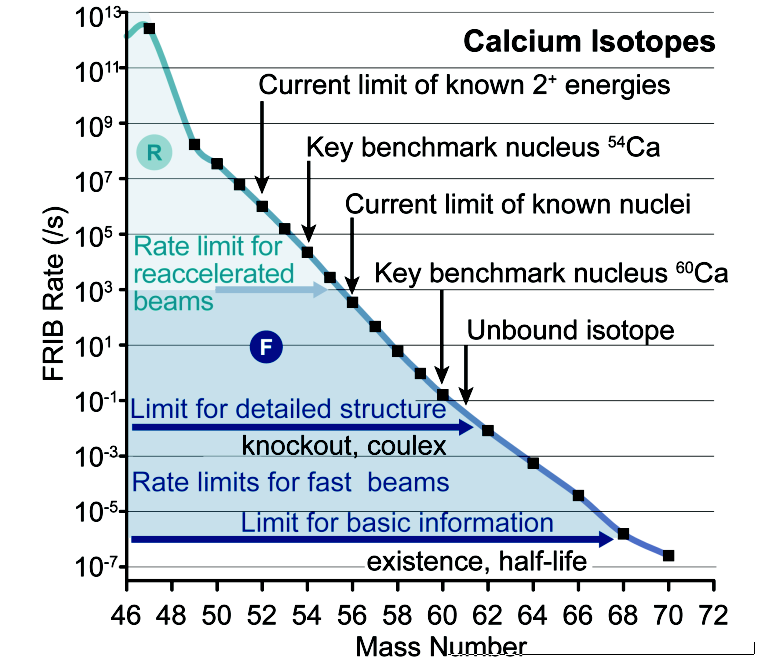
\includegraphics[width=0.6\linewidth]{fig-ch2/careach.png}}
  \caption{
  Expected experimental information on the calcium isotopes that can be obtained at FRIB. The limits for detailed spectroscopic information are around $A\sim 60$.
  }
\end{figure}
%\clearpage % flush figures 



The aim of this first section is to present some of the experimental data which can be used to extract 
information about correlations in nuclear systems. In particular, we will start with a theoretical analysis of a quantity called the separation energy for neutrons or protons. This quantity, to be discussed below, is defined as the difference between two binding energies (masses) of neighboring nuclei. As we will see from various figures below and exercises as well, the separation energies display a varying behavior as function of the number of neutrons or protons. These variations from one nucleus to another one, laid the foundation for the introduction of so-called magic numbers and a mean-field picture in order to describe nuclei theoretically.



With a mean- or average-field picture we mean that a given nucleon (either a proton or a neutron) moves in an average potential field which is set up by all other nucleons in the system. Consider for example a nucleus like $\,{}^{17}\mbox{O}$ with nine neutrons and eight protons. Many properties  of this nucleus can be interpreted in terms of a picture where we can view it as
one neutron on top of $\,{}^{16}\mbox{O}$. We infer from data and our theoretical interpretations that this additional neutron behaves almost as an individual neutron which \emph{sees} an average interaction set up by the remaining 16 nucleons in   $\,{}^{16}\mbox{O}$. A nucleus like $\,{}^{16}\mbox{O}$ is an example of what we in this course will denote as a good closed-shell nucleus. We will come back to what this means later.

Since we want to develop a theory capable of interpreting data in terms of our laws of motion and the pertinent forces,
we can think of this neutron as a particle which moves in a potential field. We can hence attempt at solving our equations of motion (Schroedinger's equation in our case) for this system along the same lines as we did in atomic physics when we solved Schroedinger's equation for the hydrogen atom. We just need to define a model for our effective single-particle potential. 

A simple potential model which enjoys quite some popularity in nuclear physics, is the three-dimensional harmonic oscillator. This potential model captures some of the physics of deeply bound single-particle states but fails in reproducing 
the less bound single-particle states. A parametrized, and more realistic,  potential model which is widely used in nuclear physics, is the so-called Woods-Saxon potential. Both the harmonic oscillator and the Woods-Saxon potential models define computational problems that can easily be solved (see below), resulting (with the appropriate parameters) in a rather good reproduction of experiment for nuclei which can be approximated as one nucleon on top (or one nucleon removed) of a so-called closed-shell system.



To be able to interpret a nucleus in such  a way requires at least that we are capable of parametrizing the abovementioned
interactions in order to reproduce say the excitation spectrum of a nucleus like $\,{}^{17}\mbox{O}$. 

With such a parametrized interaction we are able to solve Schroedinger's equation for the motion of one nucleon in a given field. A nucleus is however a true and complicated many-nucleon system, with extremely many degrees of freedom and complicated correlations, rendering the ideal solution of the many-nucleon Schroedinger equation an impossible enterprise. It is much easier to solve a single-particle problem with say a Woods-Saxon potential. Using such a potential hides however many of the complicated correlations and interactions which we see in nuclei. Such an effective single-nucleon potential is for example not capable of 
describing properties like the binding energy or the rms radius of a given nucleus. 

An improvement to these simpler single-nucleon potentials is given by the Hartree-Fock method, where the variational principle is used to define a mean-field which the nucleons move in. There are many different classes of mean-field methods.
An important difference between these methods and the simpler parametrized mean-field potentials like the harmonic oscillator and the Woods-Saxon potentials, is that the resulting equations contain information about the nuclear forces present in our models for solving Schroedinger's equation. Hartree-Fock and other mean-field methods like density functional theory form core topics in later lectures.



The aim of this section is to present some of the experimental data we will confront theory with. In particular, we will focus on separation and shell-gap energies and use these to build a picture of nuclei in terms of (from a philosophical stand we would call this  a reductionist approach) a single-particle picture. The harmonic oscillator will serve as an excellent starting point in building nuclei from the bottom and up. Here we will neglect nuclear forces, these are introduced in the next section when we discuss the Hartree-Fock method. 

The aim of this course is to develop our physics intuition of nuclear systems using  a theoretical approach  where we describe data in terms of 
the motion of individual nucleons and their mutual interactions. 

\textbf{How our theoretical pictures and models can be used to interpret data is in essence what this course is about}. Our narrative will lead us along a path where we start with single-particle models and end with the theory of the nuclear shell-model. The latter will be used to understand and analyze excitation spectra and decay patterns of nuclei, linking our theoretical understanding with interpretations of experiment. The way we build up our theoretical descriptions and interpretations follows what we may call a standard reductionistic approach, that is we start with what we believe are our effective degrees of freedom (nucleons in our case) and interactions amongst these and solve thereafter the underlying equations of motions. This defines the nuclear many-body problem, and mean-field approaches like Hartree-Fock theory and the nuclear shell-model represent different approaches to our solutions of Schroedinger's equation. 



We start our tour of experimental data and our interpretations by considering the chain of oxygen isotopes. In the exercises below you will be asked to perform similar analyses for other chains of isotopes.

The oxygen isotopes are the heaviest isotopes for which the drip line is well established.  The drip line is defined as the point where adding one more nucleon leads to an unbound nucleus. Below we will see that we can define the dripline by studying the separation energy. Where the neutron (proton) separation energy changes sign as a function of the number of neutrons (protons) defines the neutron (proton) drip line.

The oxygen isotopes are simple enough to be described by some few selected single-particle degrees of freedom.  

\begin{itemize}
\item Two out of four stable even-even isotopes exhibit a doubly magic nature, namely $\,{}^{22}\mbox{O}$ ($Z=8$, $N=14$) and $\,{}^{24}\mbox{O}$ ($Z=8$, $N=16$).

\item The structure of $\,{}^{22}\mbox{O}$ and $\,{}^{24}\mbox{O}$ is assumed to be governed by the evolution of the $1s_{1/2}$ and $0d_{5/2}$  one-quasiparticle states.

\item The isotopes $\,{}^{25}\mbox{O}$, $\,{}^{26}\mbox{O}$, $\,{}^{27}\mbox{O}$ and $\,{}^{28}\mbox{O}$ are outside the drip line, since the $0d_{3/2}$ orbit is not bound.
\end{itemize}

\noindent
 Many experiments worldwide!
These isotopes have been studied in series of recent experiments. Some of these experiments and theoretical interpretations are discussed in the following articles:

\begin{itemize}
\item $\,{}^{24}\mbox{O}$ and lighter:  C.~R.~Hoffman \emph{et al.}, Phys.~Lett.~B \textbf{672}, 17 (2009); R.~Kanungo \emph{et al}., Phys.~Rev.~Lett.~\textbf{102}, 152501 (2009); C.~R.~Hoffman \emph{et al}., Phys.~Rev.~C \textbf{83}, 031303(R) (2011); Stanoiu \emph{et al}., Phys. Rev. C \textbf{69}, 034312 (2004)

\item $\,{}^{25}\mbox{O}$: C.~R.~Hoffman \emph{et al}., Phys.~Rev.~Lett. \textbf{102},152501  (2009). 

\item $\,{}^{26}\mbox{O}$: E.~Lunderberg \emph{et al}., Phys.~Rev.~Lett. \textbf{108}, 142503 (2012). 

\item $\,{}^{26}\mbox{O}$: Z.~Kohley  \emph{et al}., Study of two-neutron radioactivity in the decay of 26O, Phys.~Rev.~Lett., \textbf{110}, 152501 (2013). 

\item Theory: Oxygen isotopes with three-body forces,  Otsuka \emph{et al}., Phys.~Rev.~Lett. \textbf{105}, 032501  (2010).  Hagen \emph{et al.}, Phys.~Rev.~Lett., \textbf{108}, 242501 (2012). 
\end{itemize}

\noindent
\section{Masses and Binding energies}
Our first approach in analyzing data theoretically, is to see if we can use experimental information to 

\begin{itemize}
\item Extract information about a \emph{so-called} single-particle  behavior

\item And interpret such a behavior in terms of the underlying forces and microscopic physics
\end{itemize}

\noindent
The next step is to see if we could use these interpretations to say something about shell closures and magic numbers. Since we focus on single-particle properties, a quantity we can extract from experiment is the separation energy for protons and neutrons. Before we proceed, we need to define quantities like masses and binding energies.   Two excellent reviews on 
recent trends in the determination of nuclear masses can be found in \href{{http://journals.aps.org/rmp/abstract/10.1103/RevModPhys.75.1021}}{\nolinkurl{http://journals.aps.org/rmp/abstract/10.1103/RevModPhys.75.1021}} and in \href{{http://iopscience.iop.org/1402-4896/2013/T152/014017/}}{\nolinkurl{http://iopscience.iop.org/1402-4896/2013/T152/014017/}}


A basic quantity which can be measured for the ground states of nuclei is the atomic mass $M(N, Z)$ of the neutral atom with atomic mass number $A$ and charge $Z$. The number of neutrons is $N$.

Atomic masses are usually tabulated in terms of the mass excess defined by
\[
\Delta M(N, Z) =  M(N, Z) - uA,
\]
where $u$ is the Atomic Mass Unit 
\[
u = M(^{12}\mathrm{C})/12 = 931.49386 \hspace{0.1cm} \mathrm{MeV}/c^2.
\]
In this course we will mainly use 
data from the 2003 compilation of Audi, Wapstra and Thibault, see \href{{http://www.sciencedirect.com/science/journal/03759474/729/1}}{\nolinkurl{http://www.sciencedirect.com/science/journal/03759474/729/1}}.


The nucleon masses are
\[
m_p = 938.27203(8)\hspace{0.1cm} \mathrm{MeV}/c^2 = 1.00727646688(13)u,
\] 
and
\[
m_n = 939.56536(8)\hspace{0.1cm} \mathrm{MeV}/c^2 = 1.0086649156(6)u.
\]

In the 2003 mass evaluation there are 2127 nuclei measured with an accuracy of 0.2
MeV or better, and 101 nuclei measured with an accuracy of greater than 0.2 MeV. For
heavy nuclei one observes several chains of nuclei with a constant $N-Z$ value whose masses are obtained from the energy released in $\alpha$-decay.


The nuclear binding energy is defined as the energy required to break up a given nucleus
into its constituent parts of $N$ neutrons and $Z$ protons. In terms of the atomic masses $M(N, Z)$ the binding energy is defined by
\[
BE(N, Z) = ZM_H c^2 + Nm_n c^2 - M(N, Z)c^2 ,
\]
where $M_H$ is the mass of the hydrogen atom and $m_n$ is the mass of the neutron.
In terms of the mass excess the binding energy is given by
\[
BE(N, Z) = Z\Delta_H c^2 + N\Delta_n c^2 -\Delta(N, Z)c^2 ,
\]
where $\Delta_H c^2 = 7.2890$ MeV and $\Delta_n c^2 = 8.0713$ MeV.


The following python program reads in the experimental data on binding energies and, stored in the file bindingenergies.dat,  plots them as function of the mass number $A$. One notices clearly a saturation of the binding energy per nucleon at $A\approx 56$.
\begin{lstlisting}[language=Python,style=blue1bar]
import numpy as np
from  matplotlib import pyplot as plt
# Load in data file
data = np.loadtxt("datafiles/bindingenergies.dat")
# Make arrays containing x-axis and binding energies as function of A
x = data[:,2]
bexpt = data[:,3]
plt.plot(x, bexpt ,'ro')
plt.axis([0,270,-1, 10.0])
plt.xlabel(r'$A$')
plt.ylabel(r'Binding energies in [MeV]')
plt.legend(('Experiment'), loc='upper right')
plt.title(r'Binding energies from experiment')
plt.savefig('expbindingenergies.pdf')
plt.savefig('expbindingenergies.png')
plt.show()
\end{lstlisting}

A popular and physically intuitive model which can be used to parametrize 
the experimental binding energies as function of $A$, is the so-called 
the liquid drop model. The ansatz is based on the following expression
\[ 
BE(N,Z) = a_1A-a_2A^{2/3}-a_3\frac{Z^2}{A^{1/3}}-a_4\frac{(N-Z)^2}{A},
\]
where $A$ stands for the number of nucleons and the $a_i$s are parameters which are determined by a fit 
to the experimental data.  

To arrive at the above expression we have assumed that we can make the following assumptions:

\begin{itemize}
 \item There is a volume term $a_1A$ proportional with the number of nucleons (the energy is also an extensive quantity). When an assembly of nucleons of the same size is packed together into the smallest volume, each interior nucleon has a certain number of other nucleons in contact with it. This contribution is proportional to the volume.

 \item There is a surface energy term $a_2A^{2/3}$. The assumption here is that a nucleon at the surface of a nucleus interacts with fewer other nucleons than one in the interior of the nucleus and hence its binding energy is less. This surface energy term takes that into account and is therefore negative and is proportional to the surface area.

 \item There is a Coulomb energy term $a_3\frac{Z^2}{A^{1/3}}$. The electric repulsion between each pair of protons in a nucleus yields less binding. 

 \item There is an asymmetry term $a_4\frac{(N-Z)^2}{A}$. This term is associated with the Pauli exclusion principle and reflectd the fact that the proton-neutron interaction is more attractive on the average than the neutron-neutron and proton-proton interactions.
\end{itemize}

\noindent
We could also add a so-called pairing term, which is a correction term that
arises from the tendency of proton pairs and neutron pairs to
occur. An even number of particles is more stable than an odd number. 
Performing a least-square fit to data, we obtain the following numerical values for the various constants
\begin{itemize}
\item $a_1=15.49$ MeV

\item $a_2=17.23$ MeV

\item $a_3=0.697$ MeV

\item $a_4=22.6$ MeV
\end{itemize}

\noindent
The python below here allows you to perform a fit of teh above parameters using nonlinear least squares curvefitting.


The following python program reads now in the experimental data on binding energies as well as the results from the above liquid drop model and plots these energies as function of the mass number $A$. One sees that for larger values of $A$, there is a better agreement with data. 
\begin{lstlisting}[language=Python,style=blue1bar]
import numpy as np
from  matplotlib import pyplot as plt
# Load in data file
data = np.loadtxt("datafiles/bindingenergies.dat")
# Make arrays containing x-axis and binding energies as function of
x = data[:,2]
bexpt = data[:,3]
liquiddrop = data[:,4]
plt.plot(x, bexpt ,'b-o', x, liquiddrop, 'r-o')
plt.axis([0,270,-1, 10.0])
plt.xlabel(r'$A$')
plt.ylabel(r'Binding energies in [MeV]')
plt.legend(('Experiment','Liquid Drop'), loc='upper right')
plt.title(r'Binding energies from experiment and liquid drop')
plt.savefig('bindingenergies.pdf')
plt.savefig('bindingenergies.png')
plt.show()
\end{lstlisting}


This  python program reads now in the experimental data on binding energies and performs a nonlinear least square fitting of the data. In the example here we use only the parameters $a_1$ and $a_2$, leaving it as an exercise to the reader to perform the fit for all four paramters. The results are plotted and compared with the experimental values.  To read more about non-linear least square methods, see for example the text of M.J. Box, D. Davies and W.H. Swann, Non-Linear optimisation Techniques, Oliver {\&} Boyd, 1969.
\begin{lstlisting}[language=Python,style=blue1bar]
import numpy as np
from scipy.optimize import curve_fit
from  matplotlib import pyplot as plt
# Load in data file
data = np.loadtxt("datafiles/bindingenergies.dat")
# Make arrays containing A on x-axis and binding energies
A = data[:,2]
bexpt = data[:,3]
# The function we want to fit to, only two terms here
def func(A,a1, a2):
    return a1*A-a2*(A**(2.0/3.0))
# function to perform nonlinear least square with guess for a1 and a2
popt, pcov = curve_fit(func, A, bexpt, p0 = (16.0, 18.0))
a1  = popt[0]
a2 = popt[1]
liquiddrop = a1*A-a2*(A**(2.0/3.0))

plt.plot(A, bexpt ,'bo', A, liquiddrop, 'ro')
plt.axis([0,270,-1, 10.0])
plt.xlabel(r'$A$')
plt.ylabel(r'Binding energies in [MeV]')
plt.legend(('Experiment','Liquid Drop'), loc='upper right')
plt.title(r'Binding energies from experiment and liquid drop')
plt.savefig('bindingenergies.pdf')
plt.savefig('bindingenergies.png')
plt.show()
\end{lstlisting}



We are now interested in interpreting experimental binding energies  in terms of a single-particle picture.
In order to do so, we  consider first energy conservation for nuclear transformations that include, for
example, the fusion of two nuclei $a$ and $b$ into the combined system $c$
\[
{^{N_a+Z_a}}a+ {^{N_b+Z_b}}b\rightarrow {^{N_c+Z_c}}c
\]
or the decay of nucleus $c$ into two other nuclei $a$ and $b$
\[
^{N_c+Z_c}c \rightarrow  ^{N_a+Z_a}a+ ^{N_b+Z_b}b
\]
In general we have the reactions
\[
\sum_i {^{N_i+Z_i}}i \rightarrow  \sum_f {^{N_f+Z_f}}f
\]
We require also that the number of protons and neutrons (the total number of nucleons) is conserved in the initial stage and final stage, unless we have processes which violate baryon conservation, 
\[
\sum_iN_i = \sum_f N_f \hspace{0.2cm}\mathrm{and} \hspace{0.2cm}\sum_iZ_i = \sum_f Z_f.
\]


\section{$Q$-values and separation energies}

The above processes can be characterized by an energy difference called the $Q$ value, defined as
\[
Q=\sum_i M(N_i, Z_i)c^2-\sum_f M(N_f, Z_f)c^2=\sum_i BE(N_f, Z_f)-\sum_i BE(N_i, Z_i)
\]
Spontaneous decay involves a single initial nuclear state and is allowed if $Q > 0$. In the decay, energy is released in the form of the kinetic energy of the final products. Reactions involving two initial nuclei are called endothermic (a net loss of energy) if $Q < 0$. The reactions are exothermic (a net release of energy) if $Q > 0$.


Let us study the Q values associated with the removal of one or two nucleons from
a nucleus. These are conventionally defined in terms of the one-nucleon and two-nucleon
separation energies. The neutron separation energy is defined as 
\[
S_n= -Q_n= BE(N,Z)-BE(N-1,Z),
\]
and the proton separation energy reads
\[
S_p= -Q_p= BE(N,Z)-BE(N,Z-1).
\]
The two-neutron separation energy is defined as
\[
S_{2n}= -Q_{2n}= BE(N,Z)-BE(N-2,Z),
\]
and  the two-proton separation energy is given by
\[
S_{2p}= -Q_{2p}= BE(N,Z)-BE(N,Z-2),
\]


Using say the neutron separation energies (alternatively the proton separation energies)
\[
S_n= -Q_n= BE(N,Z)-BE(N-1,Z),
\]
we can define the so-called energy gap for neutrons (or protons) as 
\[
\Delta S_n= BE(N,Z)-BE(N-1,Z)-\left(BE(N+1,Z)-BE(N,Z)\right),
\]
or 
\[
\Delta S_n= 2BE(N,Z)-BE(N-1,Z)-BE(N+1,Z).
\]
This quantity can in turn be used to determine which nuclei are magic or not. 
For protons we would have 
\[
\Delta S_p= 2BE(N,Z)-BE(N,Z-1)-BE(N,Z+1).
\]
We leave it as an exercise to the reader to define and interpret the two-neutron or two-proton gaps. 


The following python programs can now be used to plot the separation energies and the energy gaps for the oxygen isotopes.  The following python code reads the separation energies from file for all oxygen isotopes from $A=13$ to $A=25$, The data are taken from the file \emph{snox.dat}.  This files contains the separation energies and the shell gap energies.
\begin{lstlisting}[language=Python,style=blue1bar]

import numpy as np
from  matplotlib import pyplot as plt
# Load in data file
data = np.loadtxt("datafiles/snox.dat")
# Make arrays containing x-axis and binding energies as function of
x = data[:,1]
y = data[:,2]

plt.plot(x, y,'b-+',markersize=6)
plt.axis([4,18,-1, 25.0])
plt.xlabel(r'Number of neutrons $N$',fontsize=20)
plt.ylabel(r'$S_n$ [MeV]',fontsize=20)
plt.legend(('Separation energies for oxygen isotpes'), loc='upper right')
plt.title(r'Separation energy for the oxygen isotopes')
plt.savefig('snoxygen.pdf')
plt.savefig('snoxygen.png')
plt.show()
\end{lstlisting}


Here we display the python program for plotting the corresponding results for shell gaps for the oyxgen isotopes. 
\begin{lstlisting}[language=Python,style=blue1bar]

import numpy as np
from  matplotlib import pyplot as plt
# Load in data file
data = np.loadtxt("datafiles/snox.dat")
# Make arrays containing x-axis and binding energies as function of
x = data[:,1]
y = data[:,3]

plt.plot(x, y,'b-+',markersize=6)
plt.axis([4,18,-7, 12.0])
plt.xlabel(r'Number of neutrons $N$',fontsize=20)
plt.ylabel(r'$\Delta S_n$ [MeV]',fontsize=20)
plt.legend(('Shell gap energies for oxygen isotpes'), loc='upper right')
plt.title(r'Shell gap energies for the oxygen isotopes')
plt.savefig('gapoxygen.pdf')
plt.savefig('gapoxygen.png')
plt.show()
\end{lstlisting}





Since we will focus in the beginning on single-particle degrees of freedom and mean-field approaches before we
start with nuclear forces and many-body approaches like the nuclear shell-model, there are some features to be noted

\begin{itemize}
\item In the discussion of the liquid drop model and binding energies, we note that the total binding energy is not that different from the sum of the individual neutron and proton masses. 
\end{itemize}

\noindent
One may thus infer that intrinsic properties of nucleons in a nucleus are close to those of free nucleons.
\begin{itemize}
\item In the discussion of the neutron separation energies for the oxygen isotopes, we note  a clear staggering effect between odd and even isotopes with the even ones being more bound (larger separation energies). We will later link this to strong pairing correlations in nuclei.

\item The neutron separation energy becomes negative at $\,{}^{25}\mbox{O}$, making this nucleus unstable with respect to the emission of one neutron. A nucleus like $\,{}^{24}\mbox{O}$ is thus the last stable oxygen isotopes which has been observed. Oyxgen-26 has been found to be unbound with respect to $\,{}^{24}\mbox{O}$, see \href{{ournals.aps.org/prl/abstract/10.1103/PhysRevLett.108.142503}}{\nolinkurl{ournals.aps.org/prl/abstract/10.1103/PhysRevLett.108.142503}\footnote{\texttt{ournals.aps.org/prl/abstract/10.1103/PhysRevLett.108.142503}}} .

\item We note also that there are large shell-gaps for some nuclei, meaning that more energy is needed to remove one nucleon. These gaps are used to define so-called magic numbers. For the oxygen isotopes we see a clear gap for $\,{}^{16}\mbox{O}$. We will interpret this gap as one of several experimental properties that define so-called magic numbers. In our discussion below we will make a first interpretation using  single-particle states from the harmonic oscillator and the Woods-Saxon potential. 
\end{itemize}

\noindent
In the exercises below you will be asked to perform a similar analysis for other chains of isotopes and interpret the results. 



\section{Radii}

The root-mean-square (rms) charge radius has been measured for the ground states of many
nuclei. For a spherical charge density, $\rho(\bm{r})$, the mean-square radius is defined by
\[
\langle r^2\rangle = \frac{ \int  d \bm{r} \rho(\bm{r}) r^2}{ \int  d \bm{r} \rho(\bm{r})},
\]
and the rms radius is the square root of this quantity denoted by
\[
R =\sqrt{ \langle r^2\rangle}.
\]

Radii for most stable
nuclei have been deduced from electron scattering form
factors and/or from the x-ray transition energies of muonic atoms. 
The relative radii for a
series of isotopes can be extracted from the isotope shifts of atomic x-ray transitions.
The rms radius for the nuclear point-proton density, $R_p$ is obtained from the rms charge radius by:
\[
R_p = \sqrt{R^2_{\mathrm{ch}}- R^2_{\mathrm{corr}}},
\]
where
\[
R^2_{\mathrm{corr}}= R^2_{\mathrm{op}}+(N/Z)R^2_{\mathrm{on}}+R^2_{\mathrm{rel}},
\]
where 
\[
R_{\mathrm{op}}= 0.875(7) \mathrm{fm}.
\]
is the rms radius of the proton, $R^2_{\mathrm{on}} = 0.116(2)$ $\mbox{fm}^{2}$ is the
mean-square radius of the neutron and $R^2_{\mathrm{rel}} = 0.033$ $\mbox{fm}^{2}$ is the relativistic Darwin-Foldy correction. There are also smaller nucleus-dependent relativistic spin-orbit and
mesonic-exchange corrections that should be included.




\section{Definitions}

We will now introduce the potential models we have discussex above, namely the harmonic oscillator and the Woods-Saxon potentials.  In order to proceed, we need some definitions.

We define an operator as $\hat{O}$ throughout. Unless otherwise specified the total number of nucleons is
always $A$ and $d$ is the dimension of the system.  In nuclear physics
we normally define the total number of particles to be $A=N+Z$, where
$N$ is total number of neutrons and $Z$ the total number of
protons. In case of other baryons such as isobars $\Delta$ or various
hyperons such as $\Lambda$ or $\Sigma$, one needs to add their
definitions.  When we refer to a single neutron we will use the label $n$ and when we refer to a single proton we will use the label $p$. Unless otherwise specified, we will simply call these particles for nucleons.


The quantum numbers of a single-particle state in coordinate space are
defined by the variables 
\[
x=(\bm{r},\sigma), 
\]
where 
\[
\bm{r}\in {\mathbb{R}}^{d},
\]
with $d=1,2,3$ represents the spatial coordinates and $\sigma$ is the eigenspin of the particle. For fermions with eigenspin $1/2$ this means that
\[
 x\in {\mathbb{R}}^{d}\oplus (\frac{1}{2}),
\]
and the integral
\[
\int dx = \sum_{\sigma}\int d^dr = \sum_{\sigma}\int d\bm{r},
\]
and
\[
\int d^Ax= \int dx_1\int dx_2\dots\int dx_A.
\]
Since we are dealing with protons and neutrons we need to add isospin as a new degree of freedom.



Including isospin $\tau$ we have 
\[
x=(\bm{r},\sigma,\tau), 
\]
where 
\[
\bm{r}\in {\mathbb{R}}^{3},
\]
For nucleons, which are fermions with eigenspin $1/2$ and isospin $1/2$ this means that
\[
 x\in {\mathbb{R}}^{d}\oplus (\frac{1}{2})\oplus (\frac{1}{2}),
\]
and the integral
\[
\int dx = \sum_{\sigma\tau}\int d\bm{r},
\]
and
\[
\int d^Ax= \int dx_1\int dx_2\dots\int dx_A.
\]
We will use the standard nuclear physics definition of isospin, resulting in $\tau_z=-1/2$ for protons and $\tau_z=1/2$ for neutrons.



The quantum mechanical wave function of a given state with quantum numbers $\lambda$ (encompassing all quantum numbers needed to specify the system), ignoring time, is
\[
\Psi_{\lambda}=\Psi_{\lambda}(x_1,x_2,\dots,x_A),
\]
with $x_i=(\bm{r}_i,\sigma_i,\tau_i)$ and the projections of $\sigma_i$ and $\tau_i$ take the values
$\{-1/2,+1/2\}$. 
We will hereafter always refer to $\Psi_{\lambda}$ as the exact wave function, and if the ground state is not degenerate we label it as 
\[
\Psi_0=\Psi_0(x_1,x_2,\dots,x_A).
\]


Since the solution $\Psi_{\lambda}$ seldomly can be found in closed form, approximations are sought. In this text we define an approximative wave function or an ansatz to the exact wave function as 
\[
\Phi_{\lambda}=\Phi_{\lambda}(x_1,x_2,\dots,x_A),
\]
with

\[
\Phi_{0}=\Phi_{0}(x_{1},x_{2},\dots,x_{A}),
\]
being the ansatz for the ground state.  


The wave function $\Psi_{\lambda}$ is sought in the Hilbert space of either symmetric or anti-symmetric $N$-body functions, namely
\[
\Psi_{\lambda}\in {\cal H}_A:= {\cal H}_1\oplus{\cal H}_1\oplus\dots\oplus{\cal H}_1,
\]
where the single-particle Hilbert space $\hat{H}_1$ is the space of square integrable functions over $\in {\mathbb{R}}^{d}\oplus (\sigma)\oplus (\tau)$ resulting in
\[
{\cal H}_1:= L^2(\mathbb{R}^{d}\oplus (\sigma)\oplus (\tau)).
\]


Our Hamiltonian is invariant under the permutation (interchange) of two particles.
Since we deal with fermions however, the total wave function is antisymmetric.
Let $\hat{P}$ be an operator which interchanges two particles.
Due to the symmetries we have ascribed to our Hamiltonian, this operator commutes with the total Hamiltonian,
\[
[\hat{H},\hat{P}] = 0,
\]
meaning that $\Psi_{\lambda}(x_1, x_2, \dots , x_A)$ is an eigenfunction of 
$\hat{P}$ as well, that is
\[
\hat{P}_{ij}\Psi_{\lambda}(x_1, x_2, \dots,x_i,\dots,x_j,\dots,x_A)=
\beta\Psi_{\lambda}(x_1, x_2, \dots,x_j,\dots,x_i,\dots,x_A),
\]
where $\beta$ is the eigenvalue of $\hat{P}$. We have introduced the suffix $ij$ in order to indicate that we permute particles $i$ and $j$.
The Pauli principle tells us that the total wave function for a system of fermions
has to be antisymmetric, resulting in the eigenvalue $\beta = -1$.   



The Schrodinger equation reads 
\begin{equation}
\hat{H}(x_1, x_2, \dots , x_A) \Psi_{\lambda}(x_1, x_2, \dots , x_A) = 
E_\lambda  \Psi_\lambda(x_1, x_2, \dots , x_A), \label{eq:basicSE1}
\end{equation}
where the vector $x_i$ represents the coordinates (spatial, spin and isospin) of particle $i$, $\lambda$ stands  for all the quantum
numbers needed to classify a given $A$-particle state and $\Psi_{\lambda}$ is the pertaining eigenfunction.  Throughout this course,
$\Psi$ refers to the exact eigenfunction, unless otherwise stated.


We write the Hamilton operator, or Hamiltonian,  in a generic way 
\[
	\hat{H} = \hat{T} + \hat{V} 
\]
where $\hat{T}$  represents the kinetic energy of the system
\[
	\hat{T} = \sum_{i=1}^A \frac{\mathbf{p}_i^2}{2m_i} = \sum_{i=1}^A \left( -\frac{\hbar^2}{2m_i} \mathbf{\nabla_i}^2 \right) =
		\sum_{i=1}^A t(x_i)
\]
while the operator $\hat{V}$ for the potential energy is given by
\begin{equation}
	\hat{V} = \sum_{i=1}^A \hat{u}_{\mathrm{ext}}(x_i) + \sum_{ji=1}^A v(x_i,x_j)+\sum_{ijk=1}^Av(x_i,x_j,x_k)+\dots
\label{eq:firstv}
\end{equation}
Hereafter we use natural units, viz.~$\hbar=c=e=1$, with $e$ the elementary charge and $c$ the speed of light. This means that momenta and masses
have dimension energy. 


The potential energy part includes also an external potential $\hat{u}_{\mathrm{ext}}(x_i)$.

In a non-relativistic approach to atomic  physics, this external potential is given by the attraction an electron feels from the atomic nucleus. The latter being much heavier than the involved electrons, is often used to define a natural center of mass. In nuclear physics there is no such external potential. It is the nuclear force which results in binding in nuclear systems. In a non-relativistic framework, the nuclear force contains two-body, three-body and more complicated degrees of freedom. The potential energy reads then  
\[
	\hat{V} = \sum_{ij}^A v(x_i,x_j)+\sum_{ijk}^Av(x_i,x_j,x_k)+\dots
\]
Three-body and more  complicated forces arise since we are dealing with protons and neutrons as effective degrees of freedom. We will come back to this topic later. Furthermore, in large parts of these lectures we will assume that the potential energy can be approximated by a two-body interaction only. Our Hamiltonian reads then
\begin{equation}
	\hat{H} = \sum_{i=1}^A \frac{\mathbf{p}_i^2}{2m_i}+\sum_{ij}^A v(x_i,x_j).
\label{eq:firstH}
\end{equation}


\section{A modified Hamiltonian}

It is however, from a computational point of view, convenient to introduce an external potential $\hat{u}_{\mathrm{ext}}(x_i)$ by adding and substracting it to the original Hamiltonian. 
This means that our Hamiltonian can be rewritten as 
\[
    \hat{H} = \hat{H}_0 + \hat{H}_I 
    = \sum_{i=1}^A \hat{h}_0(x_i) + \sum_{i < j=1}^A \hat{v}(x_{ij})-\sum_{i=1}^A\hat{u}_{\mathrm{ext}}(x_i),
\]
with

\[
  \hat{H}_0=\sum_{i=1}^A \hat{h}_0(x_i) =  \sum_{i=1}^A\left(\hat{t}(x_i) + \hat{u}_{\mathrm{ext}}(x_i)\right).
\]

The interaction (or potential energy term) reads now
\[
  \hat{H}_I=  \sum_{i < j=1}^A \hat{v}(x_{ij})-\sum_{i=1}^A\hat{u}_{\mathrm{ext}}(x_i).
\]

In nuclear physics the one-body part $u_{\mathrm{ext}}(x_i)$ is often approximated by a harmonic oscillator potential or a
Woods-Saxon potential. However, this is not fully correct, because as we have discussed, nuclei are self-bound systems and there is no external confining potential. As we will see later, \emph{the $\hat{H}_0$ part of the hamiltonian cannot be used to compute the binding energy of a nucleus since it is not based on a model for the nuclear forces}. That is, the binding energy is not the sum of the individual single-particle energies. 


Why do we introduce the  Hamiltonian  in the form
\[
    \hat{H} = \hat{H}_0 + \hat{H}_I? 
\]
There are many reasons for this. Let us look at some of them, using the harmonic oscillator in three dimensions as our starting point. For the harmonic oscillator we know that

\[
  \hat{h}_0(x_i)\psi_{\alpha}(x_i)=\varepsilon_{\alpha}\psi_{\alpha}(x_i),  
\]

where the eigenvalues are $\varepsilon_{\alpha}$ and the eigenfunctions are $\psi_{\alpha}(x_i)$. The subscript $\alpha$ represents quantum numbers like the orbital angular momentum $l_{\alpha}$, its projection $m_{l_{\alpha}}$ and the   
principal quantum number $n_{\alpha}=0,1,2,\dots$. 

The eigenvalues are
\[
\varepsilon_{\alpha} = \hbar\omega \left(2n_{\alpha}+l_{\alpha}+\frac{3}{2}\right).
\]


The following mathematical properties of the  harmonic oscillator are handy. 
\begin{itemize}
 \item First of all we have a complete basis of orthogonal eigenvectors. These have well-know expressions and can be easily be encoded. 

 \item With a complete basis $\psi_{\alpha}(x_i)$, we can construct a new basis $\phi_{\tau}(x_i)$ by expanding in terms of a harmonic oscillator basis, that is  
\end{itemize}

\noindent
\[
\phi_{\tau}(x_i)=\sum_{\alpha} C_{\tau\alpha}\psi_{\alpha}(x_i),
\]
where $C_{\tau\alpha}$ represents the overlap between the two basis sets. 
\begin{itemize}
 \item As we will see later, the harmonic oscillator basis allows us to compute in an expedient way matrix elements of the interactions between two nucleons.  Using the above expansion we can in turn represent nuclear forces in terms of new basis, for example the  Woods-Saxon basis  to be discussed later here.
\end{itemize}

\noindent
The harmonic oscillator (a shifted one by a negative constant) provides also a very good approximation to most bound single-particle states. Furthermore, it serves as a starting point in building up our picture of nuclei, in particular how we define magic numbers and systems with one nucleon added to (or removed from) a closed-shell core nucleus. The figure here shows 
the various harmonic oscillator states, with those obtained with a Woods-Saxon potential as well, including a spin-orbit splitting (to be discussed below).

\begin{figure}[t]
  \centerline{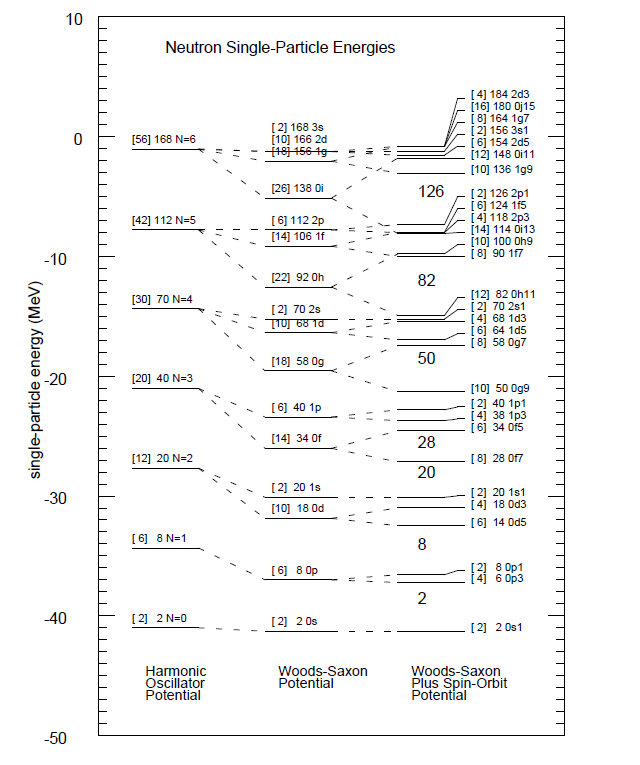
\includegraphics[width=0.6\linewidth]{fig-ch2/singleparticle.png}}
  \caption{
  Single-particle spectrum and quantum numbers for a harmonic oscillator potential and a Woods-Saxon potential with and without a spin-orbit force.
  }
\end{figure}
%\clearpage % flush figures 








In nuclear physics the one-body part $u_{\mathrm{ext}}(x_i)$ is often 
approximated by a harmonic oscillator potential. However,  as we also noted with the Woods-Saxon potential there is no 
external confining potential in nuclei. 

What many people do then, is to add and subtract a harmonic oscillator potential,
with 
\[
\hat{u}_{\mathrm{ext}}(x_i)=\hat{u}_{\mathrm{ho}}(x_i)= \frac{1}{2}m\omega^2 r_i^2,
\]
where $\omega$ is the oscillator frequency. This leads to 
\[
    \hat{H} = \hat{H_0} + \hat{H_I} 
    = \sum_{i=1}^A \hat{h}_0(x_i) + \sum_{i < j=1}^A \hat{v}(x_{ij})-\sum_{i=1}^A\hat{u}_{\mathrm{ho}}(x_i),
\]
with 
\[
  H_0=\sum_{i=1}^A \hat{h}_0(x_i) =  \sum_{i=1}^A\left(\hat{t}(x_i) + \hat{u}_{\mathrm{ho}}(x_i)\right).
\]
Many practitioners use this as the standard Hamiltonian when doing nuclear structure calculations. 
This is ok if the number of nucleons is large, but still with this Hamiltonian, we do not obey translational invariance.  How can we cure this?


 In setting up a translationally invariant Hamiltonian  
 the following expressions are helpful.
 The center-of-mass (CoM)  momentum is
\[
    P=\sum_{i=1}^A\bm{p}_i,
 \]
 and we have that
\[
 \sum_{i=1}^A\bm{p}_i^2 =
 \frac{1}{A}\left[\bm{P}^2+\sum_{i < j}(\bm{p}_i-\bm{p}_j)^2\right]
 \]
 meaning that
\[
 \left[\sum_{i=1}^A\frac{\bm{p}_i^2}{2m} -\frac{\bm{P}^2}{2mA}\right]
 =\frac{1}{2mA}\sum_{i < j}(\bm{p}_i-\bm{p}_j)^2.
 \]

 In a similar fashion we can define the CoM coordinate
\[
     \bm{R}=\frac{1}{A}\sum_{i=1}^{A}\bm{r}_i,
 \]
 which yields
 \[
 \sum_{i=1}^A\bm{r}_i^2 =
 \frac{1}{A}\left[A^2\bm{R}^2+\sum_{i < j}(\bm{r}_i-\bm{r}_j)^2\right].
 \]


 If we then introduce the harmonic oscillator one-body Hamiltonian
\[
      H_0= \sum_{i=1}^A\left(\frac{\bm{p}_i^2}{2m}+
	   \frac{1}{2}m\omega^2\bm{r}_i^2\right),
 \]
 with $\omega$ the oscillator frequency,
 we can rewrite the latter as 
 \[
      H_{\mathrm{HO}}= \frac{\bm{P}^2}{2mA}+\frac{mA\omega^2\bm{R}^2}{2}
	    +\frac{1}{2mA}\sum_{i < j}(\bm{p}_i-\bm{p}_j)^2
	    +\frac{m\omega^2}{2A}\sum_{i < j}(\bm{r}_i-\bm{r}_j)^2.
     \label{eq:obho}
 \]

Alternatively, we could write it as	
\[
 H_{\mathrm{HO}}= H_{\mathrm{CoM}}+\frac{1}{2mA}\sum_{i < j}(\bm{p}_i-\bm{p}_j)^2
	    +\frac{m\omega^2}{2A}\sum_{i < j}(\bm{r}_i-\bm{r}_j)^2,
 \]

The center-of-mass term is defined as
 \[
      H_{\mathrm{CoM}}= \frac{\bm{P}^2}{2mA}+\frac{mA\omega^2\bm{R}^2}{2}.
 \]


 The translationally invariant one- and two-body  Hamiltonian reads for an A-nucleon system,
 \[
\label{eq:ham}
\hat{H}=\left[\sum_{i=1}^A\frac{\bm{p}_i^2}{2m} -\frac{\bm{P}^2}{2mA}\right] +\sum_{i < j}^A V_{ij} \; ,
 \]
 where $V_{ij}$ is the nucleon-nucleon interaction. Adding zero as here
\[
 \sum_{i=1}^A\frac{1}{2}m\omega^2\bm{r}_i^2-
 \frac{m\omega^2}{2A}\left[\bm{R}^2+\sum_{i < j}(\bm{r}_i-\bm{r}_j)^2\right]=0.
 \]
we can then rewrite the Hamiltonian as 
\[
 \hat{H}=\sum_{i=1}^A \left[ \frac{\bm{p}_i^2}{2m}
 +\frac{1}{2}m\omega^2 \bm{r}^2_i
 \right] + \sum_{i < j}^A \left[ V_{ij}-\frac{m\omega^2}{2A}
 (\bm{r}_i-\bm{r}_j)^2
 \right]-H_{\mathrm{CoM}}.
 \]


The Woods-Saxon potential is a mean field potential for the nucleons (protons and neutrons) 
inside an atomic nucleus. It represent an average potential that a given nucleon feels from  the forces applied on each nucleon. 
The parametrization is
\[
\hat{u}_{\mathrm{ext}}(r)=-\frac{V_0}{1+\exp{(r-R)/a}},
\]
with $V_0\approx 50$ MeV representing the potential well depth, $a\approx 0.5$ fm 
length representing the "surface thickness" of the nucleus and $R=r_0A^{1/3}$, with $r_0=1.25$ fm and $A$ the number of nucleons.
The value for $r_0$ can be extracted from a fit to data, see for example M.~Kirson, \href{{http://www.sciencedirect.com/science/article/pii/S037594740600769X}}{\nolinkurl{http://www.sciencedirect.com/science/article/pii/S037594740600769X}}.

The following python code produces a plot of the Woods-Saxon potential with the above parameters. 

\begin{lstlisting}[language=Python,style=blue1bar]
import numpy as np
from  matplotlib import pyplot as plt
from matplotlib import rc, rcParams
import matplotlib.units as units
import matplotlib.ticker as ticker
rc('text',usetex=True)
rc('font',**{'family':'serif','serif':['Woods-Saxon potential']})
font = {'family' : 'serif',
        'color'  : 'darkred',
        'weight' : 'normal',
        'size'   : 16,
        }
v0 = 50
A = 100
a = 0.5
r0 = 1.25
R = r0*A**(0.3333)
x = np.linspace(0.0, 10.0)
y = -v0/(1+np.exp((x-R)/a))

plt.plot(x, y, 'b-')
plt.title(r'{\bf Woods-Saxon potential}', fontsize=20)     
plt.text(3, -40, r'Parameters: $A=20$, $V_0=50$ [MeV]', fontdict=font)
plt.text(3, -44, r'$a=0.5$ [fm], $r_0=1.25$ [fm]', fontdict=font)
plt.xlabel(r'$r$ [fm]',fontsize=20)
plt.ylabel(r'$V(r)$ [MeV]',fontsize=20)

# Tweak spacing to prevent clipping of ylabel
plt.subplots_adjust(left=0.15)
plt.savefig('woodsaxon.pdf', format='pdf')
\end{lstlisting}
From the plot we notice that the potential
\begin{itemize}
\item rapidly approaches zero as $r$ goes to infinity, reflecting the short-distance nature of the strong nuclear force.

\item For large $A$, it is approximately flat in the center.

\item Nucleons near the surface of the nucleus experience a large force towards the center.
\end{itemize}

\noindent
We have introduced a single-particle Hamiltonian
\[
  H_0=\sum_{i=1}^A \hat{h}_0(x_i) =  \sum_{i=1}^A\left(\hat{t}(x_i) + \hat{u}_{\mathrm{ext}}(x_i)\right),
\]
with an external and central symmetric potential $u_{\mathrm{ext}}(x_i)$, which is often 
approximated by a harmonic oscillator potential or a Woods-Saxon potential. Being central symmetric leads to a degeneracy 
in energy which is not observed experimentally. We see this from for example our discussion of separation energies and magic numbers. There are, in addition to the assumed magic numbers from a harmonic oscillator basis of $2,8,20,40,70\dots$ magic numbers like $28$, $50$, $82$ and $126$. 

To produce these additional numbers, we need to add a phenomenological spin-orbit force which lifts the degeneracy, that is
\[
\hat{h}(x_i) =  \hat{t}(x_i) + \hat{u}_{\mathrm{ext}}(x_i) +\xi(\bm{r})\bm{ls}=\hat{h}_0(x_i)+\xi(\bm{r})\bm{ls}. 
\]

We have introduced a modified single-particle Hamiltonian
\[
\hat{h}(x_i) =  \hat{t}(x_i) + \hat{u}_{\mathrm{ext}}(x_i) +\xi(\bm{r})\bm{ls}=\hat{h}_0(x_i)+\xi(\bm{r})\bm{ls}. 
\]
We can calculate the expectation value of the latter using the fact that
\[
\xi(\bm{r})\bm{ls}=\frac{1}{2}\xi(\bm{r})\left(\bm{j}^2-\bm{l}^2-\bm{s}^2\right).
\]
For a single-particle state with quantum numbers $nlj$ (we suppress $s$ and $m_j$), with $s=1/2$, we obtain the single-particle energies
\[
\varepsilon_{nlj} = \varepsilon_{nlj}^{(0)}+\Delta\varepsilon_{nlj}, 
\]
with $\varepsilon_{nlj}^{(0)}$ being the single-particle energy obtained with $\hat{h}_0(x)$ and
\[
\Delta\varepsilon_{nlj}=\frac{C}{2}\left(j(j+1)-l(l+1)-\frac{3}{4}\right).
\]


The spin-orbit force gives thus an additional contribution to the energy
\[
\Delta\varepsilon_{nlj}=\frac{C}{2}\left(j(j+1)-l(l+1)-\frac{3}{4}\right),
\]
which lifts the degeneracy we have seen before in the harmonic oscillator or Woods-Saxon potentials. The value $C$ is the radial
integral involving $\xi(\bm{r})$. Depending on the value of $j=l\pm 1/2$, we obtain 
\[
\Delta\varepsilon_{nlj=l-1/2}=\frac{C}{2}l,
\]
or
\[
\Delta\varepsilon_{nlj=l+1/2}=-\frac{C}{2}(l+1),
\]
clearly lifting the degeneracy. Note well that till now we have simply postulated the spin-orbit force in \emph{ad hoc} way.
Later, we will see how this term arises from the two-nucleon force in a natural way. 


With the spin-orbit force, we can modify our Woods-Saxon potential to 
\[
\hat{u}_{\mathrm{ext}}(r)=-\frac{V_0}{1+\exp{(r-R)/a}}+V_{so}(r)\bm{ls},
\]
with
\[
V_{so}(r) = V_{so}\frac{1}{r}\frac{d f_{so}(r)}{dr},
\]
where we have 
\[
f_{so}(r) = \frac{1}{1+\exp{(r-R_{so})/a_{so}}}.
\]
We can also add, in case of proton, a Coulomb potential. The Woods-Saxon potential has been widely used in parametrizations of
effective single-particle potentials. \textbf{However, as was the case with the harmonic oscillator, none of these potentials are linked directly to the nuclear forces}. Our next step is to build a mean field based on the nucleon-nucleon interaction.
This will lead us to our first and simplest many-body theory, Hartree-Fock theory.  


The Woods-Saxon potential does allow for closed-form or analytical solutions of the eigenvalue problem
\[
  \hat{h}_0(x_i)\psi_{\alpha}(x_i)=\varepsilon_{\alpha}\psi_{\alpha}(x_i).  
\]
For the harmonic oscillator in three dimensions we have closed-form expressions for the energies and analytical solutions for the eigenstates,
with the latter given by either Hermite polynomials (cartesian coordinates) or Laguerre polynomials (spherical coordinates).

To solve the above equation is however rather straightforward numerically. 



\section{Numerical solution of the single-particle Schroedinger equation}

We will illustrate the numerical solution of Schroedinger's equation by solving it for the harmonic oscillator in three dimensions.
It is straightforward to change the harmonic oscillator potential with a Woods-Saxon potential, or any other type of potentials. 

We are interested in the solution of the radial part of Schroedinger's equation for one nucleon. 
The angular momentum part  is given by the so-called Spherical harmonics. 

The radial equation reads
\[
  -\frac{\hbar^2}{2 m} \left ( \frac{1}{r^2} \frac{d}{dr} r^2
  \frac{d}{dr} - \frac{l (l + 1)}{r^2} \right )R(r) 
     + V(r) R(r) = E R(r).
\]
In our case $V(r)$ is the harmonic oscillator potential $(1/2)kr^2$ with
$k=m\omega^2$ and $E$ is
the energy of the harmonic oscillator in three dimensions.
The oscillator frequency is $\omega$ and the energies are
\[
E_{nl}=  \hbar \omega \left(2n+l+\frac{3}{2}\right),
\]
with $n=0,1,2,\dots$ and $l=0,1,2,\dots$.



Since we have made a transformation to spherical coordinates it means that 
$r\in [0,\infty)$.  
The quantum number
$l$ is the orbital momentum of the nucleon.   Then we substitute $R(r) = (1/r) u(r)$ and obtain
\[
  -\frac{\hbar^2}{2 m} \frac{d^2}{dr^2} u(r) 
       + \left ( V(r) + \frac{l (l + 1)}{r^2}\frac{\hbar^2}{2 m}
                                    \right ) u(r)  = E u(r) .
\]
The boundary conditions are $u(0)=0$ and $u(\infty)=0$.




We introduce a dimensionless variable $\rho = (1/\alpha) r$
where $\alpha$ is a constant with dimension length and get
\[
  -\frac{\hbar^2}{2 m \alpha^2} \frac{d^2}{d\rho^2} u(\rho) 
       + \left ( V(\rho) + \frac{l (l + 1)}{\rho^2}
         \frac{\hbar^2}{2 m\alpha^2} \right ) u(\rho)  = E u(\rho) .
\]
Let us specialize to $l=0$. 
Inserting $V(\rho) = (1/2) k \alpha^2\rho^2$ we end up with
\[
  -\frac{\hbar^2}{2 m \alpha^2} \frac{d^2}{d\rho^2} u(\rho) 
       + \frac{k}{2} \alpha^2\rho^2u(\rho)  = E u(\rho) .
\]
We multiply thereafter with $2m\alpha^2/\hbar^2$ on both sides and obtain
\[
  -\frac{d^2}{d\rho^2} u(\rho) 
       + \frac{mk}{\hbar^2} \alpha^4\rho^2u(\rho)  = \frac{2m\alpha^2}{\hbar^2}E u(\rho) .
\]


We have thus
\[
  -\frac{d^2}{d\rho^2} u(\rho) 
       + \frac{mk}{\hbar^2} \alpha^4\rho^2u(\rho)  = \frac{2m\alpha^2}{\hbar^2}E u(\rho) .
\]
The constant $\alpha$ can now be fixed
so that
\[
\frac{mk}{\hbar^2} \alpha^4 = 1,
\]
or 
\[
\alpha = \left(\frac{\hbar^2}{mk}\right)^{1/4}.
\]
Defining
\[
\lambda = \frac{2m\alpha^2}{\hbar^2}E,
\]
we can rewrite Schroedinger's equation as
\[
  -\frac{d^2}{d\rho^2} u(\rho) + \rho^2u(\rho)  = \lambda u(\rho) .
\]
This is the first equation to solve numerically. In three dimensions 
the eigenvalues for $l=0$ are 
$\lambda_0=3,\lambda_1=7,\lambda_2=11,\dots .$


We use the standard
expression for the second derivative of a function $u$
\begin{equation}
    u''=\frac{u(\rho+h) -2u(\rho) +u(\rho-h)}{h^2} +O(h^2),
    \label{eq:diffoperation}
\end{equation} 
where $h$ is our step.
Next we define minimum and maximum values for the variable $\rho$,
$\rho_{\mathrm{min}}=0$  and $\rho_{\mathrm{max}}$, respectively.
You need to check your results for the energies against different values
$\rho_{\mathrm{max}}$, since we cannot set
$\rho_{\mathrm{max}}=\infty$. 


With a given number of steps, $n_{\mathrm{step}}$, we then 
define the step $h$ as
\[
  h=\frac{\rho_{\mathrm{max}}-\rho_{\mathrm{min}} }{n_{\mathrm{step}}}.
\]
Define an arbitrary value of $\rho$ as 
\[
    \rho_i= \rho_{\mathrm{min}} + ih \hspace{1cm} i=0,1,2,\dots , n_{\mathrm{step}}
\]
we can rewrite the Schroedinger equation for $\rho_i$ as
\[
-\frac{u(\rho_i+h) -2u(\rho_i) +u(\rho_i-h)}{h^2}+\rho_i^2u(\rho_i)  = \lambda u(\rho_i),
\]
or in  a more compact way
\[
-\frac{u_{i+1} -2u_i +u_{i-1}}{h^2}+\rho_i^2u_i=-\frac{u_{i+1} -2u_i +u_{i-1} }{h^2}+V_iu_i  = \lambda u_i,
\]
where $V_i=\rho_i^2$ is the harmonic oscillator potential.


Define first the diagonal matrix element
\[
   d_i=\frac{2}{h^2}+V_i,
\]
and the non-diagonal matrix element 
\[
   e_i=-\frac{1}{h^2}.
\]
In this case the non-diagonal matrix elements are given by a mere constant. \emph{All non-diagonal matrix elements are equal}.

With these definitions the Schroedinger equation takes the following form
\[
d_iu_i+e_{i-1}u_{i-1}+e_{i+1}u_{i+1}  = \lambda u_i,
\]
where $u_i$ is unknown. We can write the 
latter equation as a matrix eigenvalue problem 
\begin{equation}
    \left( \begin{array}{ccccccc} d_1 & e_1 & 0   & 0    & \dots  &0     & 0 \\
                                e_1 & d_2 & e_2 & 0    & \dots  &0     &0 \\
                                0   & e_2 & d_3 & e_3  &0       &\dots & 0\\
                                \dots  & \dots & \dots & \dots  &\dots      &\dots & \dots\\
                                0   & \dots & \dots & \dots  &\dots       &d_{n_{\mathrm{step}}-2} & e_{n_{\mathrm{step}}-1}\\
                                0   & \dots & \dots & \dots  &\dots       &e_{n_{\mathrm{step}}-1} & d_{n_{\mathrm{step}}-1}

             \end{array} \right)      \left( \begin{array}{c} u_{1} \\
                                                              u_{2} \\
                                                              \dots\\ \dots\\ \dots\\
                                                              u_{n_{\mathrm{step}}-1}
             \end{array} \right)=\lambda \left( \begin{array}{c} u_{1} \\
                                                              u_{2} \\
                                                              \dots\\ \dots\\ \dots\\
                                                              u_{n_{\mathrm{step}}-1}
             \end{array} \right) 
      \label{eq:sematrix}
\end{equation} 
or if we wish to be more detailed, we can write the tridiagonal matrix as
\begin{equation}
    \left( \begin{array}{ccccccc} \frac{2}{h^2}+V_1 & -\frac{1}{h^2} & 0   & 0    & \dots  &0     & 0 \\
                                -\frac{1}{h^2} & \frac{2}{h^2}+V_2 & -\frac{1}{h^2} & 0    & \dots  &0     &0 \\
                                0   & -\frac{1}{h^2} & \frac{2}{h^2}+V_3 & -\frac{1}{h^2}  &0       &\dots & 0\\
                                \dots  & \dots & \dots & \dots  &\dots      &\dots & \dots\\
                                0   & \dots & \dots & \dots  &\dots       &\frac{2}{h^2}+V_{n_{\mathrm{step}}-2} & -\frac{1}{h^2}\\
                                0   & \dots & \dots & \dots  &\dots       &-\frac{1}{h^2} & \frac{2}{h^2}+V_{n_{\mathrm{step}}-1}

             \end{array} \right)  
\label{eq:matrixse} 
\end{equation} 
Recall that the solutions are known via the boundary conditions at
$i=n_{\mathrm{step}}$ and at the other end point, that is for  $\rho_0$.
The solution is zero in both cases.



The following python program is an example of how one can obtain the eigenvalues for a single-nucleon moving in a harmonic oscillator potential. It is rather easy to change the onebody-potential with ones like a Woods-Saxon potential. 


\begin{itemize}
\item The c++ and Fortran versions of this program can be found at \href{{https://github.com/NuclearStructure/PHY981/tree/master/doc/pub/spdata/programs}}{\nolinkurl{https://github.com/NuclearStructure/PHY981/tree/master/doc/pub/spdata/programs}}. 

\item The c++  program uses the c++ library armadillo, see \href{{http://arma.sourceforge.net/}}{\nolinkurl{http://arma.sourceforge.net/}}. 

\item To install armadillo see the guidelines at \href{{http://www.uio.no/studier/emner/matnat/fys/FYS4411/v14/guides/installing-armadillo/}}{\nolinkurl{http://www.uio.no/studier/emner/matnat/fys/FYS4411/v14/guides/installing-armadillo/}}. 

\item For mac users I recommend using \emph{brew}, see \href{{http://brew.sh/}}{\nolinkurl{http://brew.sh/}}.

\item If you use ipython notebook, you can run c++ programs following the instructions at \href{{http://nbviewer.ipython.org/github/dragly/cppmagic/blob/master/example.ipynb}}{\nolinkurl{http://nbviewer.ipython.org/github/dragly/cppmagic/blob/master/example.ipynb}}
\end{itemize}

\noindent
The code sets up the Hamiltonian matrix by defining the the minimun and maximum values of $r$ with a
maximum value of integration points.  These are set in the initialization function. It plots the 
eigenfunctions of the three lowest eigenstates.
\begin{lstlisting}[language=Python,style=blue1bar]
#Program which solves the one-particle Schrodinger equation 
#for a potential specified in function
#potential(). This example is for the harmonic oscillator in 3d

from  matplotlib import pyplot as plt
import numpy as np
#Function for initialization of parameters
def initialize():
    RMin = 0.0
    RMax = 10.0
    lOrbital = 0
    Dim = 400
    return RMin, RMax, lOrbital, Dim
# Here we set up the harmonic oscillator potential
def potential(r):
    return r*r

#Get the boundary, orbital momentum and number of integration points
RMin, RMax, lOrbital, Dim = initialize()

#Initialize constants
Step    = RMax/(Dim+1)
DiagConst = 2.0 / (Step*Step)
NondiagConst =  -1.0 / (Step*Step)
OrbitalFactor = lOrbital * (lOrbital + 1.0)

#Calculate array of potential values
v = np.zeros(Dim)
r = np.linspace(RMin,RMax,Dim)
for i in xrange(Dim):
    r[i] = RMin + (i+1) * Step;
    v[i] = potential(r[i]) + OrbitalFactor/(r[i]*r[i]);

#Setting up tridiagonal matrix and find eigenvectors and eigenvalues
Hamiltonian = np.zeros((Dim,Dim))
Hamiltonian[0,0] = DiagConst + v[0];
Hamiltonian[0,1] = NondiagConst;
for i in xrange(1,Dim-1):
    Hamiltonian[i,i-1]  = NondiagConst;
    Hamiltonian[i,i]    = DiagConst + v[i];
    Hamiltonian[i,i+1]  = NondiagConst;
Hamiltonian[Dim-1,Dim-2] = NondiagConst;
Hamiltonian[Dim-1,Dim-1] = DiagConst + v[Dim-1];
# diagonalize and obtain eigenvalues, not necessarily sorted
EigValues, EigVectors = np.linalg.eig(Hamiltonian)
# sort eigenvectors and eigenvalues
permute = EigValues.argsort()
EigValues = EigValues[permute]
EigVectors = EigVectors[:,permute]
# now plot the results for the three lowest lying eigenstates
for i in xrange(3):
    print EigValues[i]
FirstEigvector = EigVectors[:,0]
SecondEigvector = EigVectors[:,1]
ThirdEigvector = EigVectors[:,2]
plt.plot(r, FirstEigvector**2 ,'b-',r, SecondEigvector**2 ,'g-',r, ThirdEigvector**2 ,'r-')
plt.axis([0,4.6,0.0, 0.025])
plt.xlabel(r'$r$')
plt.ylabel(r'Radial probability $r^2|R(r)|^2$')
plt.title(r'Radial probability distributions for three lowest-lying states')
plt.savefig('eigenvector.pdf')
plt.savefig('eigenvector.png')
plt.show()

\end{lstlisting}





% --- begin exercise ---
\begin{doconceexercise}
\refstepcounter{doconceexercisecounter}

\subsection*{Exercise \thedoconceexercisecounter: Masses and binding energies}
\addcontentsline{loe}{doconceexercise}{Exercise \thedoconceexercisecounter: Masses and binding energies}


The data on binding energies can be found in the file bedata.dat at the github address of the course, see
\href{{https://github.com/NuclearStructure/PHY981/tree/master/doc/pub/spdata/programs}}{\nolinkurl{https://github.com/NuclearStructure/PHY981/tree/master/doc/pub/spdata/programs}}


\subex{a)}
Write a small program which reads in the proton and neutron numbers and the binding energies 
and make a plot of all neutron separation energies for the chain of oxygen (O), calcium (Ca), nickel (Ni), tin (Sn) and lead (Pb) isotopes, that is you need to plot
\[
S_n= BE(N,Z)-BE(N-1,Z).
\]
Comment your results.

\subex{b)}
In the same figures, you should also include the liquid drop model results of Eq.~(2.17) of Alex Brown's text, namely
\[
BE(N,Z)= \alpha_1A-\alpha_2A^{2/3}-\alpha_3\frac{Z^2}{A^{1/3}}-\alpha_4\frac{(N-Z)^2}{A},
\]
with $\alpha_1=15.49$ MeV, $\alpha_2=17.23$ MeV, $\alpha_3=0.697$ MeV and $\alpha_4=22.6$ MeV.
Again, comment your results.

\subex{c)}
Make also a plot of the binding energies as function of $A$ using the data in the file on binding energies and the above liquid drop model.  Make a figure similar to figure 2.5 of Alex Brown where you set the various parameters $\alpha_i=0$. Comment your results.

\subex{d)}
Use the liquid drop model to find the neutron drip lines   for Z values up to 120.
Analyze then the fluorine isotopes and find, where available the corresponding experimental data, and compare the liquid drop model predicition with experiment. 
Comment your results.
A program example in C++ and the input data file \emph{bedata.dat} can be found found at the github repository for the \href{{https://github.com/NuclearStructure/PHY981/tree/master/doc/pub/spdata/programs}}{course}\footnote{\texttt{https://github.com/NuclearStructure/PHY981/tree/master/doc/pub/spdata/programs}}



\end{doconceexercise}
% --- end exercise ---




% --- begin exercise ---
\begin{doconceexercise}
\refstepcounter{doconceexercisecounter}

\subsection*{Exercise \thedoconceexercisecounter: Eigenvalues and eigenvectors for various single-particle potentials}
\addcontentsline{loe}{doconceexercise}{Exercise \thedoconceexercisecounter: Eigenvalues and eigenvectors for various single-particle potentials}


The program for finding the eigenvalues of the harmonic oscillator are in the github folder
\href{{https://github.com/NuclearStructure/PHY981/tree/master/doc/pub/spdata/programs}}{\nolinkurl{https://github.com/NuclearStructure/PHY981/tree/master/doc/pub/spdata/programs}}.

You can use this program to solve the exercises below, or write your own using your preferred programming language, be it python, fortran or c++ or other languages. Here I will mainly provide fortran, python and c++.


\subex{a)}
Compute the eigenvalues of the five lowest states with a given orbital momentum and oscillator frequency $\omega$. Study these results as functions of the the maximum value of $r$ and the number of integration points $n$, starting with  $r_{\mathrm{max}}=10$. Compare the computed ones with the exact values and comment your results.

\subex{b)}
Plot thereafter the eigenfunctions as functions of $r$ for the lowest-lying state with a given orbital momentum $l$.

\subex{c)}
Replace thereafter the harmonic oscillator potential with a Woods-Saxon potential using the parameters discussed above. Compute the lowest five eigenvalues and plot the eigenfunction of the lowest-lying state. How does this compare with the harmonic oscillator? Comment your results and possible implications for nuclear physics studies.

\end{doconceexercise}
% --- end exercise ---




% --- begin exercise ---
\begin{doconceexercise}
\refstepcounter{doconceexercisecounter}

\subsection*{Exercise \thedoconceexercisecounter: Operators and Slater determinants}
\addcontentsline{loe}{doconceexercise}{Exercise \thedoconceexercisecounter: Operators and Slater determinants}


Consider the Slater determinant
\[
\Phi_{\lambda}^{AS}(x_{1}x_{2}\dots x_{N};\alpha_{1}\alpha_{2}\dots\alpha_{N})
=\frac{1}{\sqrt{N!}}\sum_{p}(-)^{p}P\prod_{i=1}^{N}\psi_{\alpha_{i}}(x_{i}).
\]
where $P$ is an operator which permutes the coordinates of two particles. We have assumed here that the 
number of particles is the same as the number of available single-particle states, represented by the
greek letters $\alpha_{1}\alpha_{2}\dots\alpha_{N}$.


\subex{a)}
Write  out $\Phi^{AS}$ for $N=3$.

\subex{b)}
Show that
\[
\int dx_{1}dx_{2}\dots dx_{N}\left\vert
\Phi_{\lambda}^{AS}(x_{1}x_{2}\dots x_{N};\alpha_{1}\alpha_{2}\dots\alpha_{N})
\right\vert^{2} = 1.
\]

\subex{c)}
Define a general onebody operator $\hat{F} = \sum_{i}^N\hat{f}(x_{i})$ and a general  twobody operator $\hat{G}=\sum_{i>j}^N\hat{g}(x_{i},x_{j})$ with $g$ being invariant under the interchange of the coordinates of particles $i$ and $j$. Calculate the matrix elements for a two-particle Slater determinant
\[
\langle\Phi_{\alpha_{1}\alpha_{2}}^{AS}|\hat{F}|\Phi_{\alpha_{1}\alpha_{2}}^{AS}\rangle,
\]
and
\[
\langle\Phi_{\alpha_{1}\alpha_{2}}^{AS}|\hat{G}|\Phi_{\alpha_{1}\alpha_{2}}^{AS}\rangle.
\]
Explain the short-hand notation for the Slater determinant.
Which properties do you expect these operators to have in addition to an eventual permutation
symmetry?


\end{doconceexercise}
% --- end exercise ---




% --- begin exercise ---
\begin{doconceexercise}
\refstepcounter{doconceexercisecounter}

\subsection*{Exercise \thedoconceexercisecounter: First simple shell-model calculation}
\addcontentsline{loe}{doconceexercise}{Exercise \thedoconceexercisecounter: First simple shell-model calculation}


We will now consider a simple three-level problem, depicted in the figure below. This is our first and very simple model of a possible many-nucleon (or just fermion) problem and the shell-model.
The single-particle states are labelled by the quantum number $p$ and can accomodate up to two single particles,  viz., every single-particle state  is doubly degenerate (you could think of this as one state having spin up and the other spin down). 
We let the spacing between the doubly degenerate single-particle states be constant, with value $d$.  The first state
has energy $d$. There are only three available single-particle states, $p=1$, $p=2$ and $p=3$, as illustrated
in the figure.


\subex{a)}
How many two-particle Slater determinants can we construct in this space? 

We limit ourselves to a system with only the two lowest single-particle orbits and two particles, $p=1$ and $p=2$. We assume that we can write the Hamiltonian as
\[
       \hat{H}=\hat{H}_0+\hat{H}_I,
\]
and that the onebody part of the Hamiltonian with single-particle operator $\hat{h}_0$ has the property
\[
\hat{h}_0\psi_{p\sigma} = p\times d \psi_{p\sigma},
\]
where we have added a spin quantum number $\sigma$. 
We assume also that the only two-particle states that can exist are those where two particles are in the 
same state $p$, as shown by the two possibilities to the left in the figure.
The two-particle matrix elements of $\hat{H}_I$ have all a constant value, $-g$.

\subex{b)}
Show then that the Hamiltonian matrix can be written as 
\[
\left(\begin{array}{cc}2d-g &-g \\
-g &4d-g \end{array}\right),
\]

\subex{c)}
Find the eigenvalues and eigenvectors.  What is mixing of the state with two particles in $p=2$  to the wave function with two-particles in $p=1$? Discuss your results in terms of a linear combination of Slater determinants.

\subex{d)}
Add the possibility that the two particles can be in the state with $p=3$ as well and find the Hamiltonian matrix, the eigenvalues and the eigenvectors. We still insist that we only have two-particle states composed of two particles being in the same level $p$. You can diagonalize numerically your $3\times 3$ matrix.
This simple model catches several birds with a stone. It demonstrates how we can build linear combinations
of Slater determinants and interpret these as different admixtures to a given state. It represents also the way we are going to interpret these contributions.  The two-particle states above $p=1$ will be interpreted as 
excitations from the ground state configuration, $p=1$ here.  The reliability of this ansatz for the ground state, 
with two particles in $p=1$,
depends on the strength of the interaction $g$ and the single-particle spacing $d$.
Finally, this model is a simple schematic ansatz for studies of pairing correlations and thereby superfluidity/superconductivity  
in fermionic systems. 


\begin{figure}[t]
  \centerline{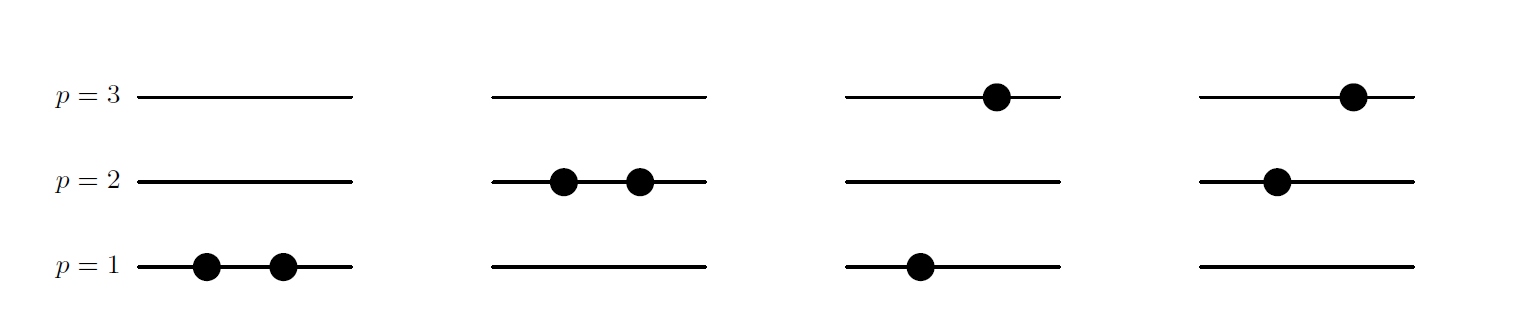
\includegraphics[width=0.6\linewidth]{fig-ch2/simplemodel.png}}
  \caption{
  Schematic plot of the possible single-particle levels with double degeneracy. The filled circles indicate occupied particle states. The spacing between each level $p$ is constant in this picture. We show some possible two-particle states.
  }
\end{figure}
%\clearpage % flush figures 




\end{doconceexercise}
% --- end exercise ---


% !split
\chapter{Mean-field approaches}
\label{ch:meanfield}

\section{Derivation of Hartree-Fock equations in coordinate space}

Hartree-Fock (HF) theory is an algorithm for finding an approximative expression for the ground state of a given Hamiltonian. The basic ingredients are
\begin{itemize}
  \item Define a single-particle basis $\{\psi_{\alpha}\}$ so that
\end{itemize}

\noindent
\[ 
\hat{h}^{\mathrm{HF}}\psi_{\alpha} = \varepsilon_{\alpha}\psi_{\alpha}
\]
with the Hartree-Fock Hamiltonian defined as
\[
\hat{h}^{\mathrm{HF}}=\hat{t}+\hat{u}_{\mathrm{ext}}+\hat{u}^{\mathrm{HF}}
\]
\begin{itemize}
  \item The term  $\hat{u}^{\mathrm{HF}}$ is a single-particle potential to be determined by the HF algorithm.

  \item The HF algorithm means to choose $\hat{u}^{\mathrm{HF}}$ in order to have 
\end{itemize}

\noindent
\[ \langle \hat{H} \rangle = E^{\mathrm{HF}}= \langle \Phi_0 | \hat{H}|\Phi_0 \rangle
\]
that is to find a local minimum with a Slater determinant $\Phi_0$ being the ansatz for the ground state. 
\begin{itemize}
  \item The variational principle ensures that $E^{\mathrm{HF}} \ge E_0$, with $E_0$ the exact ground state energy.
\end{itemize}

\noindent
We will show that the Hartree-Fock Hamiltonian $\hat{h}^{\mathrm{HF}}$ equals our definition of the operator $\hat{f}$ discussed in connection with the new definition of the normal-ordered Hamiltonian (see later lectures), that is we have, for a specific matrix element
\[
\langle p |\hat{h}^{\mathrm{HF}}| q \rangle =\langle p |\hat{f}| q \rangle=\langle p|\hat{t}+\hat{u}_{\mathrm{ext}}|q \rangle +\sum_{i\le F} \langle pi | \hat{V} | qi\rangle_{AS},
\]
meaning that
\[
\langle p|\hat{u}^{\mathrm{HF}}|q\rangle = \sum_{i\le F} \langle pi | \hat{V} | qi\rangle_{AS}.
\]
The so-called Hartree-Fock potential $\hat{u}^{\mathrm{HF}}$ brings an explicit medium dependence due to the summation over all single-particle states below the Fermi level $F$. It brings also in an explicit dependence on the two-body interaction (in nuclear physics we can also have complicated three- or higher-body forces). The two-body interaction, with its contribution from the other bystanding fermions, creates an effective mean field in which a given fermion moves, in addition to the external potential $\hat{u}_{\mathrm{ext}}$ which confines the motion of the fermion. For systems like nuclei, there is no external confining potential. Nuclei are examples of self-bound systems, where the binding arises due to the intrinsic nature of the strong force. For nuclear systems thus, there would be no external one-body potential in the Hartree-Fock Hamiltonian. 


The calculus of variations involves 
problems where the quantity to be minimized or maximized is an integral. 

In the general case we have an integral of the type
\[ 
E[\Phi]= \int_a^b f(\Phi(x),\frac{\partial \Phi}{\partial x},x)dx,
\]
where $E$ is the quantity which is sought minimized or maximized.
The problem is that although $f$ is a function of the variables $\Phi$, $\partial \Phi/\partial x$ and $x$, the exact dependence of
$\Phi$ on $x$ is not known.  This means again that even though the integral has fixed limits $a$ and $b$, the path of integration is
not known. In our case the unknown quantities are the single-particle wave functions and we wish to choose an integration path which makes
the functional $E[\Phi]$ stationary. This means that we want to find minima, or maxima or saddle points. In physics we search normally for minima.
Our task is therefore to find the minimum of $E[\Phi]$ so that its variation $\delta E$ is zero  subject to specific
constraints. In our case the constraints appear as the integral which expresses the orthogonality of the  single-particle wave functions.
The constraints can be treated via the technique of Lagrangian multipliers



Let us specialize to the expectation value of the energy for one particle in three-dimensions.
This expectation value reads
\[
  E=\int dxdydz \psi^*(x,y,z) \hat{H} \psi(x,y,z),
\]
with the constraint
\[
 \int dxdydz \psi^*(x,y,z) \psi(x,y,z)=1,
\]
and a Hamiltonian
\[
\hat{H}=-\frac{1}{2}\nabla^2+V(x,y,z).
\]
We will, for the sake of notational convenience,  skip the variables $x,y,z$ below, and write for example $V(x,y,z)=V$.



The integral involving the kinetic energy can be written as, with the function $\psi$ vanishing
strongly for large values of $x,y,z$ (given here by the limits $a$ and $b$), 
 \[
  \int_a^b dxdydz \psi^* \left(-\frac{1}{2}\nabla^2\right) \psi dxdydz = \psi^*\nabla\psi|_a^b+\int_a^b dxdydz\frac{1}{2}\nabla\psi^*\nabla\psi.
\]
We will drop the limits $a$ and $b$ in the remaining discussion. 
Inserting this expression into the expectation value for the energy and taking the variational minimum  we obtain
\[
\delta E = \delta \left\{\int dxdydz\left( \frac{1}{2}\nabla\psi^*\nabla\psi+V\psi^*\psi\right)\right\} = 0.
\]



The constraint appears in integral form as 
\[
 \int dxdydz \psi^* \psi=\mathrm{constant},
\]
and multiplying with a Lagrangian multiplier $\lambda$ and taking the variational minimum we obtain the final variational equation
\[
\delta \left\{\int dxdydz\left( \frac{1}{2}\nabla\psi^*\nabla\psi+V\psi^*\psi-\lambda\psi^*\psi\right)\right\} = 0.
\]
We introduce the function  $f$
\[
  f =  \frac{1}{2}\nabla\psi^*\nabla\psi+V\psi^*\psi-\lambda\psi^*\psi=
\frac{1}{2}(\psi^*_x\psi_x+\psi^*_y\psi_y+\psi^*_z\psi_z)+V\psi^*\psi-\lambda\psi^*\psi,
\]
where we have skipped the dependence on $x,y,z$ and introduced the shorthand $\psi_x$, $\psi_y$ and $\psi_z$  for the various derivatives.




For $\psi^*$ the Euler-Lagrange  equations yield
\[
\frac{\partial f}{\partial \psi^*}- \frac{\partial }{\partial x}\frac{\partial f}{\partial \psi^*_x}-\frac{\partial }{\partial y}\frac{\partial f}{\partial \psi^*_y}-\frac{\partial }{\partial z}\frac{\partial f}{\partial \psi^*_z}=0,
\] 
which results in 
\[
    -\frac{1}{2}(\psi_{xx}+\psi_{yy}+\psi_{zz})+V\psi=\lambda \psi.
\]
We can then identify the  Lagrangian multiplier as the energy of the system. The last equation is 
nothing but the standard 
Schroedinger equation and the variational  approach discussed here provides 
a powerful method for obtaining approximate solutions of the wave function.






\section{Definitions and notations}

Before we proceed we need some definitions.
We will assume that the interacting part of the Hamiltonian
can be approximated by a two-body interaction.
This means that our Hamiltonian is written as the sum of some onebody part and a twobody part
\begin{equation}
    \hat{H} = \hat{H}_0 + \hat{H}_I 
    = \sum_{i=1}^A \hat{h}_0(x_i) + \sum_{i < j}^A \hat{v}(r_{ij}),
\label{Hnuclei}
\end{equation}
with 
\begin{equation}
  H_0=\sum_{i=1}^A \hat{h}_0(x_i).
\label{hinuclei}
\end{equation}
The onebody part $u_{\mathrm{ext}}(x_i)$ is normally approximated by a harmonic oscillator potential or the Coulomb interaction an electron feels from the nucleus. However, other potentials are fully possible, such as 
one derived from the self-consistent solution of the Hartree-Fock equations to be discussed here.




Our Hamiltonian is invariant under the permutation (interchange) of two particles.
Since we deal with fermions however, the total wave function is antisymmetric.
Let $\hat{P}$ be an operator which interchanges two particles.
Due to the symmetries we have ascribed to our Hamiltonian, this operator commutes with the total Hamiltonian,
\[
[\hat{H},\hat{P}] = 0,
 \]
meaning that $\Psi_{\lambda}(x_1, x_2, \dots , x_A)$ is an eigenfunction of 
$\hat{P}$ as well, that is
\[
\hat{P}_{ij}\Psi_{\lambda}(x_1, x_2, \dots,x_i,\dots,x_j,\dots,x_A)=
\beta\Psi_{\lambda}(x_1, x_2, \dots,x_i,\dots,x_j,\dots,x_A),
\]
where $\beta$ is the eigenvalue of $\hat{P}$. We have introduced the suffix $ij$ in order to indicate that we permute particles $i$ and $j$.
The Pauli principle tells us that the total wave function for a system of fermions
has to be antisymmetric, resulting in the eigenvalue $\beta = -1$.   



In our case we assume that  we can approximate the exact eigenfunction with a Slater determinant
\begin{equation}
   \Phi(x_1, x_2,\dots ,x_A,\alpha,\beta,\dots, \sigma)=\frac{1}{\sqrt{A!}}
\left| \begin{array}{ccccc} \psi_{\alpha}(x_1)& \psi_{\alpha}(x_2)& \dots & \dots & \psi_{\alpha}(x_A)\\
                            \psi_{\beta}(x_1)&\psi_{\beta}(x_2)& \dots & \dots & \psi_{\beta}(x_A)\\  
                            \dots & \dots & \dots & \dots & \dots \\
                            \dots & \dots & \dots & \dots & \dots \\
                     \psi_{\sigma}(x_1)&\psi_{\sigma}(x_2)& \dots & \dots & \psi_{\sigma}(x_A)\end{array} \right|, \label{eq:HartreeFockDet}
\end{equation}
where  $x_i$  stand for the coordinates and spin values of a particle $i$ and $\alpha,\beta,\dots, \gamma$ 
are quantum numbers needed to describe remaining quantum numbers.  



The single-particle function $\psi_{\alpha}(x_i)$  are eigenfunctions of the onebody
Hamiltonian $h_i$, that is
\[
\hat{h}_0(x_i)=\hat{t}(x_i) + \hat{u}_{\mathrm{ext}}(x_i),
\]
with eigenvalues 
\[
\hat{h}_0(x_i) \psi_{\alpha}(x_i)=\left(\hat{t}(x_i) + \hat{u}_{\mathrm{ext}}(x_i)\right)\psi_{\alpha}(x_i)=\varepsilon_{\alpha}\psi_{\alpha}(x_i).
\]
The energies $\varepsilon_{\alpha}$ are the so-called non-interacting single-particle energies, or unperturbed energies. 
The total energy is in this case the sum over all  single-particle energies, if no two-body or more complicated
many-body interactions are present.



Let us denote the ground state energy by $E_0$. According to the
variational principle we have
\[
  E_0 \le E[\Phi] = \int \Phi^*\hat{H}\Phi d\mathbf{\tau}
\]
where $\Phi$ is a trial function which we assume to be normalized
\[
  \int \Phi^*\Phi d\mathbf{\tau} = 1,
\]
where we have used the shorthand $d\mathbf{\tau}=dx_1dr_2\dots dr_A$.



In the Hartree-Fock method the trial function is the Slater
determinant of Eq.~(\ref{eq:HartreeFockDet}) which can be rewritten as 
\[
  \Phi(x_1,x_2,\dots,x_A,\alpha,\beta,\dots,\nu) = \frac{1}{\sqrt{A!}}\sum_{P} (-)^P\hat{P}\psi_{\alpha}(x_1)
    \psi_{\beta}(x_2)\dots\psi_{\nu}(x_A)=\sqrt{A!}\hat{A}\Phi_H,
\]
where we have introduced the antisymmetrization operator $\hat{A}$ defined by the 
summation over all possible permutations of two particles.


It is defined as
\begin{equation}
  \hat{A} = \frac{1}{A!}\sum_{p} (-)^p\hat{P},
\label{antiSymmetryOperator}
\end{equation}
with $p$ standing for the number of permutations. We have introduced for later use the so-called
Hartree-function, defined by the simple product of all possible single-particle functions
\[
  \Phi_H(x_1,x_2,\dots,x_A,\alpha,\beta,\dots,\nu) =
  \psi_{\alpha}(x_1)
    \psi_{\beta}(x_2)\dots\psi_{\nu}(x_A).
\]



Both $\hat{H}_0$ and $\hat{H}_I$ are invariant under all possible permutations of any two particles
and hence commute with $\hat{A}$
\begin{equation}
  [H_0,\hat{A}] = [H_I,\hat{A}] = 0. \label{commutionAntiSym}
\end{equation}
Furthermore, $\hat{A}$ satisfies
\begin{equation}
  \hat{A}^2 = \hat{A},  \label{AntiSymSquared}
\end{equation}
since every permutation of the Slater
determinant reproduces it. 




The expectation value of $\hat{H}_0$ 
\[
  \int \Phi^*\hat{H}_0\Phi d\mathbf{\tau} 
  = A! \int \Phi_H^*\hat{A}\hat{H}_0\hat{A}\Phi_H d\mathbf{\tau}
\]
is readily reduced to
\[
  \int \Phi^*\hat{H}_0\Phi d\mathbf{\tau} 
  = A! \int \Phi_H^*\hat{H}_0\hat{A}\Phi_H d\mathbf{\tau},
\]
where we have used Eqs.~(\ref{commutionAntiSym}) and
(\ref{AntiSymSquared}). The next step is to replace the antisymmetrization
operator by its definition and to
replace $\hat{H}_0$ with the sum of one-body operators
\[
  \int \Phi^*\hat{H}_0\Phi  d\mathbf{\tau}
  = \sum_{i=1}^A \sum_{p} (-)^p\int 
  \Phi_H^*\hat{h}_0\hat{P}\Phi_H d\mathbf{\tau}.
\]



The integral vanishes if two or more particles are permuted in only one
of the Hartree-functions $\Phi_H$ because the individual single-particle wave functions are
orthogonal. We obtain then
\[
  \int \Phi^*\hat{H}_0\Phi  d\mathbf{\tau}= \sum_{i=1}^A \int \Phi_H^*\hat{h}_0\Phi_H  d\mathbf{\tau}.
\]
Orthogonality of the single-particle functions allows us to further simplify the integral, and we
arrive at the following expression for the expectation values of the
sum of one-body Hamiltonians 
\begin{equation}
  \int \Phi^*\hat{H}_0\Phi  d\mathbf{\tau}
  = \sum_{\mu=1}^A \int \psi_{\mu}^*(x)\hat{h}_0\psi_{\mu}(x)dx
  d\mathbf{r}.
  \label{H1Expectation}
\end{equation}



We introduce the following shorthand for the above integral
\[
\langle \mu | \hat{h}_0 | \mu \rangle = \int \psi_{\mu}^*(x)\hat{h}_0\psi_{\mu}(x)dx,
\]
and rewrite Eq.~(\ref{H1Expectation}) as
\begin{equation}
  \int \Phi^*\hat{H}_0\Phi  d\tau
  = \sum_{\mu=1}^A \langle \mu | \hat{h}_0 | \mu \rangle.
  \label{H1Expectation1}
\end{equation}



The expectation value of the two-body part of the Hamiltonian is obtained in a
similar manner. We have
\[
  \int \Phi^*\hat{H}_I\Phi d\mathbf{\tau} 
  = A! \int \Phi_H^*\hat{A}\hat{H}_I\hat{A}\Phi_H d\mathbf{\tau},
\]
which reduces to
\[
 \int \Phi^*\hat{H}_I\Phi d\mathbf{\tau} 
  = \sum_{i\le j=1}^A \sum_{p} (-)^p\int 
  \Phi_H^*\hat{v}(r_{ij})\hat{P}\Phi_H d\mathbf{\tau},
\]
by following the same arguments as for the one-body
Hamiltonian. 



Because of the dependence on the inter-particle distance $r_{ij}$,  permutations of
any two particles no longer vanish, and we get
\[
  \int \Phi^*\hat{H}_I\Phi d\mathbf{\tau} 
  = \sum_{i < j=1}^A \int  
  \Phi_H^*\hat{v}(r_{ij})(1-P_{ij})\Phi_H d\mathbf{\tau}.
\]
where $P_{ij}$ is the permutation operator that interchanges
particle $i$ and particle $j$. Again we use the assumption that the single-particle wave functions
are orthogonal. 





We obtain
\begin{equation}
\begin{split}
  \int \Phi^*\hat{H}_I\Phi d\mathbf{\tau} 
  = \frac{1}{2}\sum_{\mu=1}^A\sum_{\nu=1}^A
    &\left[ \int \psi_{\mu}^*(x_i)\psi_{\nu}^*(x_j)\hat{v}(r_{ij})\psi_{\mu}(x_i)\psi_{\nu}(x_j)
    dx_idx_j \right.\\
  &\left.
  - \int \psi_{\mu}^*(x_i)\psi_{\nu}^*(x_j)
  \hat{v}(r_{ij})\psi_{\nu}(x_i)\psi_{\mu}(x_j)
  dx_idx_j
  \right]. \label{H2Expectation}
\end{split}
\end{equation}
The first term is the so-called direct term. It is frequently also called the  Hartree term, 
while the second is due to the Pauli principle and is called
the exchange term or just the Fock term.
The factor  $1/2$ is introduced because we now run over
all pairs twice. 



The last equation allows us to  introduce some further definitions.  
The single-particle wave functions $\psi_{\mu}(x)$, defined by the quantum numbers $\mu$ and $x$
are defined as the overlap 
\[
   \psi_{\alpha}(x)  = \langle x | \alpha \rangle .
\]


We introduce the following shorthands for the above two integrals
\[
\langle \mu\nu|\hat{v}|\mu\nu\rangle =  \int \psi_{\mu}^*(x_i)\psi_{\nu}^*(x_j)\hat{v}(r_{ij})\psi_{\mu}(x_i)\psi_{\nu}(x_j)
    dx_idx_j,
\]
and
\[
\langle \mu\nu|\hat{v}|\nu\mu\rangle = \int \psi_{\mu}^*(x_i)\psi_{\nu}^*(x_j)
  \hat{v}(r_{ij})\psi_{\nu}(x_i)\psi_{\mu}(x_j)
  dx_idx_j.  
\]












\section{Derivation of Hartree-Fock equations in coordinate space}

Let us denote the ground state energy by $E_0$. According to the
variational principle we have
\[
  E_0 \le E[\Phi] = \int \Phi^*\hat{H}\Phi d\mathbf{\tau}
\]
where $\Phi$ is a trial function which we assume to be normalized
\[
  \int \Phi^*\Phi d\mathbf{\tau} = 1,
\]
where we have used the shorthand $d\mathbf{\tau}=dx_1dx_2\dots dx_A$.





In the Hartree-Fock method the trial function is a Slater
determinant which can be rewritten as 
\[
  \Psi(x_1,x_2,\dots,x_A,\alpha,\beta,\dots,\nu) = \frac{1}{\sqrt{A!}}\sum_{P} (-)^PP\psi_{\alpha}(x_1)
    \psi_{\beta}(x_2)\dots\psi_{\nu}(x_A)=\sqrt{A!}\hat{A}\Phi_H,
\]
where we have introduced the anti-symmetrization operator $\hat{A}$ defined by the 
summation over all possible permutations \emph{p} of two fermions.
It is defined as
\[
  \hat{A} = \frac{1}{A!}\sum_{p} (-)^p\hat{P},
\]
with the the Hartree-function given by the simple product of all possible single-particle function
\[
  \Phi_H(x_1,x_2,\dots,x_A,\alpha,\beta,\dots,\nu) =
  \psi_{\alpha}(x_1)
    \psi_{\beta}(x_2)\dots\psi_{\nu}(x_A).
\]




Our functional is written as
\[
  E[\Phi] = \sum_{\mu=1}^A \int \psi_{\mu}^*(x_i)\hat{h}_0(x_i)\psi_{\mu}(x_i) dx_i 
  + \frac{1}{2}\sum_{\mu=1}^A\sum_{\nu=1}^A
   \left[ \int \psi_{\mu}^*(x_i)\psi_{\nu}^*(x_j)\hat{v}(r_{ij})\psi_{\mu}(x_i)\psi_{\nu}(x_j)dx_idx_j- \int \psi_{\mu}^*(x_i)\psi_{\nu}^*(x_j)
 \hat{v}(r_{ij})\psi_{\nu}(x_i)\psi_{\mu}(x_j)dx_idx_j\right]
\]
The more compact version reads
\[
  E[\Phi] 
  = \sum_{\mu}^A \langle \mu | \hat{h}_0 | \mu\rangle+ \frac{1}{2}\sum_{\mu\nu}^A\left[\langle \mu\nu |\hat{v}|\mu\nu\rangle-\langle \nu\mu |\hat{v}|\mu\nu\rangle\right].
\]



Since the interaction is invariant under the interchange of two particles it means for example that we have
\[
\langle \mu\nu|\hat{v}|\mu\nu\rangle =  \langle \nu\mu|\hat{v}|\nu\mu\rangle,  
\]
or in the more general case
\[
\langle \mu\nu|\hat{v}|\sigma\tau\rangle =  \langle \nu\mu|\hat{v}|\tau\sigma\rangle.  
\]



The direct and exchange matrix elements can be  brought together if we define the antisymmetrized matrix element
\[
\langle \mu\nu|\hat{v}|\mu\nu\rangle_{AS}= \langle \mu\nu|\hat{v}|\mu\nu\rangle-\langle \mu\nu|\hat{v}|\nu\mu\rangle,
\]
or for a general matrix element  
\[
\langle \mu\nu|\hat{v}|\sigma\tau\rangle_{AS}= \langle \mu\nu|\hat{v}|\sigma\tau\rangle-\langle \mu\nu|\hat{v}|\tau\sigma\rangle.
\]
It has the symmetry property
\[
\langle \mu\nu|\hat{v}|\sigma\tau\rangle_{AS}= -\langle \mu\nu|\hat{v}|\tau\sigma\rangle_{AS}=-\langle \nu\mu|\hat{v}|\sigma\tau\rangle_{AS}.
\]
The antisymmetric matrix element is also hermitian, implying 
\[
\langle \mu\nu|\hat{v}|\sigma\tau\rangle_{AS}= \langle \sigma\tau|\hat{v}|\mu\nu\rangle_{AS}.
\]



With these notations we rewrite the Hartree-Fock functional as
\begin{equation}
  \int \Phi^*\hat{H_I}\Phi d\mathbf{\tau} 
  = \frac{1}{2}\sum_{\mu=1}^A\sum_{\nu=1}^A \langle \mu\nu|\hat{v}|\mu\nu\rangle_{AS}. \label{H2Expectation2}
\end{equation}

Adding the contribution from the one-body operator $\hat{H}_0$ to
(\ref{H2Expectation2}) we obtain the energy functional 
\begin{equation}
  E[\Phi] 
  = \sum_{\mu=1}^A \langle \mu | h | \mu \rangle +
  \frac{1}{2}\sum_{{\mu}=1}^A\sum_{{\nu}=1}^A \langle \mu\nu|\hat{v}|\mu\nu\rangle_{AS}. \label{FunctionalEPhi}
\end{equation}
In our coordinate space derivations below we will spell out the Hartree-Fock equations in terms of their integrals.




If we generalize the Euler-Lagrange equations to more variables 
and introduce $N^2$ Lagrange multipliers which we denote by 
$\epsilon_{\mu\nu}$, we can write the variational equation for the functional of $E$
\[
  \delta E - \sum_{\mu\nu}^A \epsilon_{\mu\nu} \delta
  \int \psi_{\mu}^* \psi_{\nu} = 0.
\]
For the orthogonal wave functions $\psi_{i}$ this reduces to
\[
  \delta E - \sum_{\mu=1}^A \epsilon_{\mu} \delta
  \int \psi_{\mu}^* \psi_{\mu} = 0.
\]




Variation with respect to the single-particle wave functions $\psi_{\mu}$ yields then
\[
  \sum_{\mu=1}^A \int \delta\psi_{\mu}^*\hat{h_0}(x_i)\psi_{\mu}
  dx_i  
  + \frac{1}{2}\sum_{{\mu}=1}^A\sum_{{\nu}=1}^A \left[ \int
  \delta\psi_{\mu}^*\psi_{\nu}^*\hat{v}(r_{ij})\psi_{\mu}\psi_{\nu} dx_idx_j- \int
  \delta\psi_{\mu}^*\psi_{\nu}^*\hat{v}(r_{ij})\psi_{\nu}\psi_{\mu}
  dx_idx_j \right]+ 
\]
\[
\sum_{\mu=1}^A \int \psi_{\mu}^*\hat{h_0}(x_i)\delta\psi_{\mu}
  dx_i 
  + \frac{1}{2}\sum_{{\mu}=1}^A\sum_{{\nu}=1}^A \left[ \int
  \psi_{\mu}^*\psi_{\nu}^*\hat{v}(r_{ij})\delta\psi_{\mu}\psi_{\nu} dx_idx_j- \int
  \psi_{\mu}^*\psi_{\nu}^*\hat{v}(r_{ij})\psi_{\nu}\delta\psi_{\mu}
  dx_idx_j \right]-  \sum_{{\mu}=1}^A E_{\mu} \int \delta\psi_{\mu}^*
  \psi_{\mu}dx_i
  -  \sum_{{\mu}=1}^A E_{\mu} \int \psi_{\mu}^*
  \delta\psi_{\mu}dx_i = 0.
\]




Although the variations $\delta\psi$ and $\delta\psi^*$ are not
independent, they may in fact be treated as such, so that the 
terms dependent on either $\delta\psi$ and $\delta\psi^*$ individually 
may be set equal to zero. To see this, simply 
replace the arbitrary variation $\delta\psi$ by $i\delta\psi$, so that
$\delta\psi^*$ is replaced by $-i\delta\psi^*$, and combine the two
equations. We thus arrive at the Hartree-Fock equations
\begin{equation}
\left[ -\frac{1}{2}\nabla_i^2+ \sum_{\nu=1}^A\int \psi_{\nu}^*(x_j)\hat{v}(r_{ij})\psi_{\nu}(x_j)dx_j \right]\psi_{\mu}(x_i) - \left[ \sum_{{\nu}=1}^A \int\psi_{\nu}^*(x_j)\hat{v}(r_{ij})\psi_{\mu}(x_j) dx_j\right] \psi_{\nu}(x_i) = \epsilon_{\mu} \psi_{\mu}(x_i).  \label{eq:hartreefockcoordinatespace}
\end{equation}
Notice that the integration $\int dx_j$ implies an
integration over the spatial coordinates $\mathbf{r_j}$ and a summation
over the spin-coordinate of fermion $j$. We note that the factor of $1/2$ in front of the sum involving the two-body interaction, has been removed. This is due to the fact that we need to vary both $\delta\psi_{\mu}^*$ and
$\delta\psi_{\nu}^*$. Using the symmetry properties of the two-body interaction and interchanging $\mu$ and $\nu$
as summation indices, we obtain two identical terms. 




The two first terms in the last equation are the one-body kinetic energy and the
electron-nucleus potential. The third or \emph{direct} term is the averaged electronic repulsion of the other
electrons. As written, the
term includes the \emph{self-interaction} of 
electrons when $\mu=\nu$. The self-interaction is cancelled in the fourth
term, or the \emph{exchange} term. The exchange term results from our
inclusion of the Pauli principle and the assumed determinantal form of
the wave-function. Equation (\ref{eq:hartreefockcoordinatespace}), in addition to the kinetic energy and the attraction from the atomic nucleus that confines the motion of a single electron,   represents now the motion of a single-particle modified by the two-body interaction. The additional contribution to the Schroedinger equation due to the two-body interaction, represents a mean field set up by all the other bystanding electrons, the latter given by the sum over all single-particle states occupied by $N$ electrons. 

The Hartree-Fock equation is an example of an integro-differential equation. These equations involve repeated calculations of integrals, in addition to the solution of a set of coupled differential equations. 
The Hartree-Fock equations can also be rewritten in terms of an eigenvalue problem. The solution of an eigenvalue problem represents often a more practical algorithm and the  solution of  coupled  integro-differential equations.
This alternative derivation of the Hartree-Fock equations is given below.




\section{Analysis of Hartree-Fock equations in coordinate space}

  A theoretically convenient form of the
Hartree-Fock equation is to regard the direct and exchange operator
defined through 
\begin{equation*}
  V_{\mu}^{d}(x_i) = \int \psi_{\mu}^*(x_j) 
 \hat{v}(r_{ij})\psi_{\mu}(x_j) dx_j
\end{equation*}
and
\begin{equation*}
  V_{\mu}^{ex}(x_i) g(x_i) 
  = \left(\int \psi_{\mu}^*(x_j) 
 \hat{v}(r_{ij})g(x_j) dx_j
  \right)\psi_{\mu}(x_i),
\end{equation*}
respectively. 



The function $g(x_i)$ is an arbitrary function,
and by the substitution $g(x_i) = \psi_{\nu}(x_i)$
we get
\begin{equation*}
  V_{\mu}^{ex}(x_i) \psi_{\nu}(x_i) 
  = \left(\int \psi_{\mu}^*(x_j) 
 \hat{v}(r_{ij})\psi_{\nu}(x_j)
  dx_j\right)\psi_{\mu}(x_i).
\end{equation*}
We may then rewrite the Hartree-Fock equations as
\[
  \hat{h}^{HF}(x_i) \psi_{\nu}(x_i) = \epsilon_{\nu}\psi_{\nu}(x_i),
\]
with
\[
  \hat{h}^{HF}(x_i)= \hat{h}_0(x_i) + \sum_{\mu=1}^AV_{\mu}^{d}(x_i) -
  \sum_{\mu=1}^AV_{\mu}^{ex}(x_i),
\]
and where $\hat{h}_0(i)$ is the one-body part. The latter is normally chosen as a part which yields solutions in closed form. The harmonic oscilltor is a classical problem thereof.
We normally rewrite the last equation as
\[
  \hat{h}^{HF}(x_i)= \hat{h}_0(x_i) + \hat{u}^{HF}(x_i). 
\]




\section{Hartree-Fock by varying the coefficients of a wave function expansion}

Another possibility is to expand the single-particle functions in a known basis  and vary the coefficients, 
that is, the new single-particle wave function is written as a linear expansion
in terms of a fixed chosen orthogonal basis (for example the well-known harmonic oscillator functions or the hydrogen-like functions etc).
We define our new Hartree-Fock single-particle basis by performing a unitary transformation 
on our previous basis (labelled with greek indices) as
\begin{equation}
\psi_p^{HF}  = \sum_{\lambda} C_{p\lambda}\phi_{\lambda}. \label{eq:newbasis}
\end{equation}
In this case we vary the coefficients $C_{p\lambda}$. If the basis has infinitely many solutions, we need
to truncate the above sum.  We assume that the basis $\phi_{\lambda}$ is orthogonal. A unitary transformation keeps the orthogonality, as discussed in exercise 1 below.  


It is normal to choose a single-particle basis defined as the eigenfunctions
of parts of the full Hamiltonian. The typical situation consists of the solutions of the one-body part of the Hamiltonian, that is we have
\[
\hat{h}_0\phi_{\lambda}=\epsilon_{\lambda}\phi_{\lambda}.
\]
The single-particle wave functions $\phi_{\lambda}({\bf r})$, defined by the quantum numbers $\lambda$ and ${\bf r}$
are defined as the overlap 
\[
   \phi_{\lambda}({\bf r})  = \langle {\bf r} | \lambda \rangle .
\]



In our discussions hereafter we will use our definitions of single-particle states above and below the Fermi ($F$) level given by the labels
$ijkl\dots \le F$ for so-called single-hole states and $abcd\dots > F$ for so-called particle states.
For general single-particle states we employ the labels $pqrs\dots$. 




In Eq.~(\ref{FunctionalEPhi}), restated here
\[
  E[\Phi] 
  = \sum_{\mu=1}^A \langle \mu | h | \mu \rangle +
  \frac{1}{2}\sum_{{\mu}=1}^A\sum_{{\nu}=1}^A \langle \mu\nu|\hat{v}|\mu\nu\rangle_{AS},
\]
we found the expression for the energy functional in terms of the basis function $\phi_{\lambda}({\bf r})$. We then  varied the above energy functional with respect to the basis functions $|\mu \rangle$. 
Now we are interested in defining a new basis defined in terms of
a chosen basis as defined in Eq.~(\ref{eq:newbasis}). We can then rewrite the energy functional as
\begin{equation}
  E[\Phi^{HF}] 
  = \sum_{i=1}^A \langle i | h | i \rangle +
  \frac{1}{2}\sum_{ij=1}^A\langle ij|\hat{v}|ij\rangle_{AS}, \label{FunctionalEPhi2}
\end{equation}
where $\Phi^{HF}$ is the new Slater determinant defined by the new basis of Eq.~(\ref{eq:newbasis}). 


Using Eq.~(\ref{eq:newbasis}) we can rewrite Eq.~(\ref{FunctionalEPhi2}) as 
\begin{equation}
  E[\Psi] 
  = \sum_{i=1}^A \sum_{\alpha\beta} C^*_{i\alpha}C_{i\beta}\langle \alpha | h | \beta \rangle +
  \frac{1}{2}\sum_{ij=1}^A\sum_{{\alpha\beta\gamma\delta}} C^*_{i\alpha}C^*_{j\beta}C_{i\gamma}C_{j\delta}\langle \alpha\beta|\hat{v}|\gamma\delta\rangle_{AS}. \label{FunctionalEPhi3}
\end{equation}


We wish now to minimize the above functional. We introduce again a set of Lagrange multipliers, noting that
since $\langle i | j \rangle = \delta_{i,j}$ and $\langle \alpha | \beta \rangle = \delta_{\alpha,\beta}$, 
the coefficients $C_{i\gamma}$ obey the relation
\[
 \langle i | j \rangle=\delta_{i,j}=\sum_{\alpha\beta} C^*_{i\alpha}C_{i\beta}\langle \alpha | \beta \rangle=
\sum_{\alpha} C^*_{i\alpha}C_{i\alpha},
\]
which allows us to define a functional to be minimized that reads
\begin{equation}
  F[\Phi^{HF}]=E[\Phi^{HF}] - \sum_{i=1}^A\epsilon_i\sum_{\alpha} C^*_{i\alpha}C_{i\alpha}.
\end{equation}

Minimizing with respect to $C^*_{i\alpha}$, remembering that the equations for $C^*_{i\alpha}$ and $C_{i\alpha}$
can be written as two  independent equations, we obtain
\[
\frac{d}{dC^*_{i\alpha}}\left[  E[\Phi^{HF}] - \sum_{j}\epsilon_j\sum_{\alpha} C^*_{j\alpha}C_{j\alpha}\right]=0,
\]
which yields for every single-particle state $i$ and index $\alpha$ (recalling that the coefficients $C_{i\alpha}$ are matrix elements of a unitary (or orthogonal for a real symmetric matrix) matrix)
the following Hartree-Fock equations
\[
\sum_{\beta} C_{i\beta}\langle \alpha | h | \beta \rangle+
\sum_{j=1}^A\sum_{\beta\gamma\delta} C^*_{j\beta}C_{j\delta}C_{i\gamma}\langle \alpha\beta|\hat{v}|\gamma\delta\rangle_{AS}=\epsilon_i^{HF}C_{i\alpha}.
\]



We can rewrite this equation as (changing dummy variables)
\[
\sum_{\beta} \left\{\langle \alpha | h | \beta \rangle+
\sum_{j}^A\sum_{\gamma\delta} C^*_{j\gamma}C_{j\delta}\langle \alpha\gamma|\hat{v}|\beta\delta\rangle_{AS}\right\}C_{i\beta}=\epsilon_i^{HF}C_{i\alpha}.
\]
Note that the sums over greek indices run over the number of basis set functions (in principle an infinite number).

Defining 
\[
h_{\alpha\beta}^{HF}=\langle \alpha | h | \beta \rangle+
\sum_{j=1}^A\sum_{\gamma\delta} C^*_{j\gamma}C_{j\delta}\langle \alpha\gamma|\hat{v}|\beta\delta\rangle_{AS},
\]
we can rewrite the new equations as 
\begin{equation}
\sum_{\gamma}h_{\alpha\beta}^{HF}C_{i\beta}=\epsilon_i^{HF}C_{i\alpha}. \label{eq:newhf}
\end{equation}
The latter is nothing but a standard eigenvalue problem. Compared with Eq.~(\ref{eq:hartreefockcoordinatespace}),
we see that we do not need to compute any integrals in an iterative procedure for solving the equations.
It suffices to tabulate the matrix elements $\langle \alpha | h | \beta \rangle$ and $\langle \alpha\gamma|\hat{v}|\beta\delta\rangle_{AS}$ once and for all. Successive iterations require thus only a look-up in tables over one-body and two-body matrix elements. These details will be discussed below when we solve the Hartree-Fock equations numerical. 



Our Hartree-Fock matrix  is thus
\[
\hat{h}_{\alpha\beta}^{HF}=\langle \alpha | \hat{h}_0 | \beta \rangle+
\sum_{j=1}^A\sum_{\gamma\delta} C^*_{j\gamma}C_{j\delta}\langle \alpha\gamma|\hat{v}|\beta\delta\rangle_{AS}.
\]
The Hartree-Fock equations are solved in an iterative waym starting with a guess for the coefficients $C_{j\gamma}=\delta_{j,\gamma}$ and solving the equations by diagonalization till the new single-particle energies
$\epsilon_i^{\mathrm{HF}}$ do not change anymore by a prefixed quantity. 



Normally we assume that the single-particle basis $|\beta\rangle$ forms an eigenbasis for the operator
$\hat{h}_0$, meaning that the Hartree-Fock matrix becomes  
\[
\hat{h}_{\alpha\beta}^{HF}=\epsilon_{\alpha}\delta_{\alpha,\beta}+
\sum_{j=1}^A\sum_{\gamma\delta} C^*_{j\gamma}C_{j\delta}\langle \alpha\gamma|\hat{v}|\beta\delta\rangle_{AS}.
\]
The Hartree-Fock eigenvalue problem
\[
\sum_{\beta}\hat{h}_{\alpha\beta}^{HF}C_{i\beta}=\epsilon_i^{\mathrm{HF}}C_{i\alpha},
\]
can be written out in a more compact form as
\[
\hat{h}^{HF}\hat{C}=\epsilon^{\mathrm{HF}}\hat{C}. 
\]



\section{Hartree-Fock algorithm}

The Hartree-Fock equations are, in their simplest form, solved in an iterative way, starting with a guess for the
coefficients $C_{i\alpha}$. We label the coefficients as $C_{i\alpha}^{(n)}$, where the subscript $n$ stands for iteration $n$.
To set up the algorithm we can proceed as follows:

\begin{itemize}
 \item We start with a guess $C_{i\alpha}^{(0)}=\delta_{i,\alpha}$. Alternatively, we could have used random starting values as long as the vectors are normalized. Another possibility is to give states below the Fermi level a larger weight.

 \item The Hartree-Fock matrix simplifies then to (assuming that the coefficients $C_{i\alpha} $  are real)
\end{itemize}

\noindent
\[
\hat{h}_{\alpha\beta}^{HF}=\epsilon_{\alpha}\delta_{\alpha,\beta}+
\sum_{j = 1}^A\sum_{\gamma\delta} C_{j\gamma}^{(0)}C_{j\delta}^{(0)}\langle \alpha\gamma|\hat{v}|\beta\delta\rangle_{AS}.
\]


Solving the Hartree-Fock eigenvalue problem yields then new eigenvectors $C_{i\alpha}^{(1)}$ and eigenvalues
$\epsilon_i^{HF(1)}$. 
\begin{itemize}
 \item With the new eigenvalues we can set up a new Hartree-Fock potential 
\end{itemize}

\noindent
\[
\sum_{j = 1}^A\sum_{\gamma\delta} C_{j\gamma}^{(1)}C_{j\delta}^{(1)}\langle \alpha\gamma|\hat{v}|\beta\delta\rangle_{AS}.
\]
The diagonalization with the new Hartree-Fock potential yields new eigenvectors and eigenvalues.
This process is continued till for example
\[
\frac{\sum_{p} |\epsilon_i^{(n)}-\epsilon_i^{(n-1)}|}{m} \le \lambda,  
\]
where $\lambda$ is a user prefixed quantity ($\lambda \sim 10^{-8}$ or smaller) and $p$ runs over all calculated single-particle
energies and $m$ is the number of single-particle states.



\section{Analysis of Hartree-Fock equations and Koopman's theorem}

We can rewrite the ground state energy by adding and subtracting $\hat{u}^{HF}(x_i)$ 
\[
  E_0^{HF} =\langle \Phi_0 | \hat{H} | \Phi_0\rangle = 
\sum_{i\le F}^A \langle i | \hat{h}_0 +\hat{u}^{HF}| j\rangle+ \frac{1}{2}\sum_{i\le F}^A\sum_{j \le F}^A\left[\langle ij |\hat{v}|ij \rangle-\langle ij|\hat{v}|ji\rangle\right]-\sum_{i\le F}^A \langle i |\hat{u}^{HF}| i\rangle,
\]
which results in
\[
  E_0^{HF}
  = \sum_{i\le F}^A \varepsilon_i^{HF} + \frac{1}{2}\sum_{i\le F}^A\sum_{j \le F}^A\left[\langle ij |\hat{v}|ij \rangle-\langle ij|\hat{v}|ji\rangle\right]-\sum_{i\le F}^A \langle i |\hat{u}^{HF}| i\rangle.
\]
Our single-particle states $ijk\dots$ are now single-particle states obtained from the solution of the Hartree-Fock equations.


Using our definition of the Hartree-Fock single-particle energies we obtain then the following expression for the total ground-state energy
\[
  E_0^{HF}
  = \sum_{i\le F}^A \varepsilon_i - \frac{1}{2}\sum_{i\le F}^A\sum_{j \le F}^A\left[\langle ij |\hat{v}|ij \rangle-\langle ij|\hat{v}|ji\rangle\right].
\]
This form will be used in our discussion of Koopman's theorem.


We have 
\[
  E[\Phi^{\mathrm{HF}}(N)] 
  = \sum_{i=1}^H \langle i | \hat{h}_0 | i \rangle +
  \frac{1}{2}\sum_{ij=1}^N\langle ij|\hat{v}|ij\rangle_{AS},
\]
where $\Phi^{\mathrm{HF}}(N)$ is the new Slater determinant defined by the new basis of Eq.~(\ref{eq:newbasis})
for $N$ electrons (same $Z$).  If we assume that the single-particle wave functions in the new basis do not change 
when we remove one electron or add one electron, we can then define the corresponding energy for the $N-1$ systems as 
\[
  E[\Phi^{\mathrm{HF}}(N-1)] 
  = \sum_{i=1; i\ne k}^N \langle i | \hat{h}_0 | i \rangle +
  \frac{1}{2}\sum_{ij=1;i,j\ne k}^N\langle ij|\hat{v}|ij\rangle_{AS},
\]
where we have removed a single-particle state $k\le F$, that is a state below the Fermi level.  


Calculating the difference 
\[
  E[\Phi^{\mathrm{HF}}(N)]-   E[\Phi^{\mathrm{HF}}(N-1)] = \langle k | \hat{h}_0 | k \rangle +
  \frac{1}{2}\sum_{i=1;i\ne k}^N\langle ik|\hat{v}|ik\rangle_{AS}  \frac{1}{2}\sum_{j=1;j\ne k}^N\langle kj|\hat{v}|kj\rangle_{AS},
\]
we obtain
\[
  E[\Phi^{\mathrm{HF}}(N)]-   E[\Phi^{\mathrm{HF}}(N-1)] = \langle k | \hat{h}_0 | k \rangle +
  \frac{1}{2}\sum_{j=1}^N\langle kj|\hat{v}|kj\rangle_{AS}
\]
which is just our definition of the Hartree-Fock single-particle energy
\[
  E[\Phi^{\mathrm{HF}}(N)]-   E[\Phi^{\mathrm{HF}}(N-1)] = \epsilon_k^{\mathrm{HF}} 
\]

Similarly, we can now compute the difference (we label the single-particle states above the Fermi level as $abcd > F$)
\[
  E[\Phi^{\mathrm{HF}}(N+1)]-   E[\Phi^{\mathrm{HF}}(N)]= \epsilon_a^{\mathrm{HF}}. 
\]
These two equations can thus be used to the electron affinity or ionization energies, respectively. 
Koopman's theorem states that for example the ionization energy of a closed-shell system is given by the energy of the highest occupied single-particle state.  If we assume that changing the number of electrons from $N$ to $N+1$ does not change the Hartree-Fock single-particle energies and eigenfunctions, then Koopman's theorem simply states that the ionization energy of an atom is given by the single-particle energy of the last bound state. In a similar way, we can also define the electron affinities. 



As an example, consider a simple model for atomic sodium, Na. Neutral sodium has eleven electrons, 
with the weakest bound one being confined the $3s$ single-particle quantum numbers. The energy needed to remove an electron from neutral sodium is rather small, 5.1391 eV, a feature which pertains to all alkali metals.
Having performed a  Hartree-Fock calculation for neutral sodium would then allows us to compute the
ionization energy by using the single-particle energy for the $3s$ states, namely $\epsilon_{3s}^{\mathrm{HF}}$. 

From these considerations, we see that Hartree-Fock theory allows us to make a connection between experimental 
observables (here ionization and affinity energies) and the underlying interactions between particles.  
In this sense, we are now linking the dynamics and structure of a many-body system with the laws of motion which govern the system. Our approach is a reductionistic one, meaning that we want to understand the laws of motion 
in terms of the particles or degrees of freedom which we believe are the fundamental ones. Our Slater determinant, being constructed as the product of various single-particle functions, follows this philosophy.


With similar arguments as in atomic physics, we can now use Hartree-Fock theory to make a link
between nuclear forces and separation energies. Changing to nuclear system, we define
\[
  E[\Phi^{\mathrm{HF}}(A)] 
  = \sum_{i=1}^A \langle i | \hat{h}_0 | i \rangle +
  \frac{1}{2}\sum_{ij=1}^A\langle ij|\hat{v}|ij\rangle_{AS},
\]
where $\Phi^{\mathrm{HF}}(A)$ is the new Slater determinant defined by the new basis of Eq.~(\ref{eq:newbasis})
for $A$ nucleons, where $A=N+Z$, with $N$ now being the number of neutrons and $Z$ th enumber of protons.  If we assume again that the single-particle wave functions in the new basis do not change from a nucleus with $A$ nucleons to a nucleus with $A-1$  nucleons, we can then define the corresponding energy for the $A-1$ systems as 
\[
  E[\Phi^{\mathrm{HF}}(A-1)] 
  = \sum_{i=1; i\ne k}^A \langle i | \hat{h}_0 | i \rangle +
  \frac{1}{2}\sum_{ij=1;i,j\ne k}^A\langle ij|\hat{v}|ij\rangle_{AS},
\]
where we have removed a single-particle state $k\le F$, that is a state below the Fermi level.  


Calculating the difference 
\[
  E[\Phi^{\mathrm{HF}}(A)]-   E[\Phi^{\mathrm{HF}}(A-1)] 
  = \langle k | \hat{h}_0 | k \rangle +
  \frac{1}{2}\sum_{i=1;i\ne k}^A\langle ik|\hat{v}|ik\rangle_{AS}  \frac{1}{2}\sum_{j=1;j\ne k}^A\langle kj|\hat{v}|kj\rangle_{AS},
\]
which becomes 
\[
  E[\Phi^{\mathrm{HF}}(A)]-   E[\Phi^{\mathrm{HF}}(A-1)] 
  = \langle k | \hat{h}_0 | k \rangle +
  \frac{1}{2}\sum_{j=1}^A\langle kj|\hat{v}|kj\rangle_{AS}
\]
which is just our definition of the Hartree-Fock single-particle energy
\[
  E[\Phi^{\mathrm{HF}}(A)]-   E[\Phi^{\mathrm{HF}}(A-1)] 
  = \epsilon_k^{\mathrm{HF}} 
\]


Similarly, we can now compute the difference (recall that the single-particle states $abcd > F$)
\[
  E[\Phi^{\mathrm{HF}}(A+1)]-   E[\Phi^{\mathrm{HF}}(A)]= \epsilon_a^{\mathrm{HF}}. 
\]
If we then recall that the binding energy differences 
\[
BE(A)-BE(A-1) \hspace{0.5cm} \mathrm{and} \hspace{0.5cm} BE(A+1)-BE(A), 
\]
define the separation energies, we see that the Hartree-Fock single-particle energies can be used to
define separation energies. We have thus our first link between nuclear forces (included in the potential energy term) and an observable quantity defined by differences in binding energies. 


We have thus the following interpretations (if the single-particle field do not change)
\[
BE(A)-BE(A-1)\approx  E[\Phi^{\mathrm{HF}}(A)]-   E[\Phi^{\mathrm{HF}}(A-1)] 
  = \epsilon_k^{\mathrm{HF}}, 
\]
and
\[
BE(A+1)-BE(A)\approx  E[\Phi^{\mathrm{HF}}(A+1)]-   E[\Phi^{\mathrm{HF}}(A)] =  \epsilon_a^{\mathrm{HF}}. 
\]
If  we use ${}^{16}\mbox{O}$ as our closed-shell nucleus, we could then interpret the separation energy
\[
BE(^{16}\mathrm{O})-BE(^{15}\mathrm{O})\approx \epsilon_{0p^{\nu}_{1/2}}^{\mathrm{HF}}, 
\]
and
\[
BE(^{16}\mathrm{O})-BE(^{15}\mathrm{N})\approx \epsilon_{0p^{\pi}_{1/2}}^{\mathrm{HF}}.
\]


Similalry, we could interpret
\[
BE(^{17}\mathrm{O})-BE(^{16}\mathrm{O})\approx \epsilon_{0d^{\nu}_{5/2}}^{\mathrm{HF}}, 
\]
and 
\[
BE(^{17}\mathrm{F})-BE(^{16}\mathrm{O})\approx\epsilon_{0d^{\pi}_{5/2}}^{\mathrm{HF}}.
\]
We can continue like this for all $A\pm 1$ nuclei where $A$ is a good closed-shell (or subshell closure)
nucleus. Examples are ${}^{22}\mbox{O}$, ${}^{24}\mbox{O}$, ${}^{40}\mbox{Ca}$, ${}^{48}\mbox{Ca}$, ${}^{52}\mbox{Ca}$, ${}^{54}\mbox{Ca}$, ${}^{56}\mbox{Ni}$, 
${}^{68}\mbox{Ni}$, ${}^{78}\mbox{Ni}$, ${}^{90}\mbox{Zr}$, ${}^{88}\mbox{Sr}$, ${}^{100}\mbox{Sn}$, ${}^{132}\mbox{Sn}$ and ${}^{208}\mbox{Pb}$, to mention some possile cases.


We can thus make our first interpretation of the separation energies in terms of the simplest
possible many-body theory. 
If we also recall that the so-called energy gap for neutrons (or protons) is defined as
\[
\Delta S_n= 2BE(N,Z)-BE(N-1,Z)-BE(N+1,Z),
\]
for neutrons and the corresponding gap for protons
\[
\Delta S_p= 2BE(N,Z)-BE(N,Z-1)-BE(N,Z+1),
\]
we can define the neutron and proton energy gaps for ${}^{16}\mbox{O}$ as
\[
\Delta S_{\nu}=\epsilon_{0d^{\nu}_{5/2}}^{\mathrm{HF}}-\epsilon_{0p^{\nu}_{1/2}}^{\mathrm{HF}}, 
\]
and 
\[
\Delta S_{\pi}=\epsilon_{0d^{\pi}_{5/2}}^{\mathrm{HF}}-\epsilon_{0p^{\pi}_{1/2}}^{\mathrm{HF}}. 
\]






% --- begin exercise ---
\begin{doconceexercise}
\refstepcounter{doconceexercisecounter}

\subsection*{Exercise \thedoconceexercisecounter: Derivation of Hartree-Fock equations}
\addcontentsline{loe}{doconceexercise}{Exercise \thedoconceexercisecounter: Derivation of Hartree-Fock equations}


Consider a Slater determinant built up of single-particle orbitals $\psi_{\lambda}$, 
with $\lambda = 1,2,\dots,N$.

The unitary transformation
\[
\psi_a  = \sum_{\lambda} C_{a\lambda}\phi_{\lambda},
\]
brings us into the new basis.  
The new basis has quantum numbers $a=1,2,\dots,N$.


\subex{a)}
Show that the new basis is orthonormal.

\subex{b)}
Show that the new Slater determinant constructed from the new single-particle wave functions can be
written as the determinant based on the previous basis and the determinant of the matrix $C$.

\subex{c)}
Show that the old and the new Slater determinants are equal up to a complex constant with absolute value unity.

% --- begin hint in exercise ---

\paragraph{Hint.}
Hint, $C$ is a unitary matrix.

% --- end hint in exercise ---



\end{doconceexercise}
% --- end exercise ---




% --- begin exercise ---
\begin{doconceexercise}
\refstepcounter{doconceexercisecounter}

\subsection*{Exercise \thedoconceexercisecounter: Derivation of Hartree-Fock equations}
\addcontentsline{loe}{doconceexercise}{Exercise \thedoconceexercisecounter: Derivation of Hartree-Fock equations}


Consider the  Slater  determinant
\[
\Phi_{0}=\frac{1}{\sqrt{n!}}\sum_{p}(-)^{p}P
\prod_{i=1}^{n}\psi_{\alpha_{i}}(x_{i}).
\]
A small variation in this function is given by
\[
\delta\Phi_{0}=\frac{1}{\sqrt{n!}}\sum_{p}(-)^{p}P
\psi_{\alpha_{1}}(x_{1})\psi_{\alpha_{2}}(x_{2})\dots
\psi_{\alpha_{i-1}}(x_{i-1})(\delta\psi_{\alpha_{i}}(x_{i}))
\psi_{\alpha_{i+1}}(x_{i+1})\dots\psi_{\alpha_{n}}(x_{n}).
\]


\subex{a)}
Show that
\begin{align*}
\langle \delta\Phi_{0}|\sum_{i=1}^{n}\left\{t(x_{i})+u(x_{i})
\right\}+\frac{1}{2}
\sum_{i\neq j=1}^{n}v(x_{i},x_{j})|\Phi_{0}\rangle & =\sum_{i=1}^{n}\langle \delta\psi_{\alpha_{i}}|\hat{t}+\hat{u}
|\phi_{\alpha_{i}}\rangle \\
&+\sum_{i\neq j=1}^{n}\left\{\langle\delta\psi_{\alpha_{i}}
\psi_{\alpha_{j}}|\hat{v}|\psi_{\alpha_{i}}\psi_{\alpha_{j}}\rangle-
\langle\delta\psi_{\alpha_{i}}\psi_{\alpha_{j}}|\hat{v}
|\psi_{\alpha_{j}}\psi_{\alpha_{i}}\rangle\right\}
\end{align*}









\end{doconceexercise}
% --- end exercise ---


% !split
\chapter{Second quantization}
\label{ch:squant}


\section{Second quantization}
\begin{itemize}
\item Second quantization and operators, two-body operator with examples 

\item Wick's theorem (missing in html and ipython notebook but in pdf files)

\item Thouless' theorem and analysis of the Hartree-Fock equations using second quantization

\item Examples on how to use bit representations for Slater determinants

\item TO DO: add material about Wick's theorem and diagrammatic representation

\item TO DO: Link determinantal analysis with Thouless' theorem
\end{itemize}

\noindent
We introduce the time-independent  operators
$a_\alpha^{\dagger}$ and $a_\alpha$   which create and annihilate, respectively, a particle 
in the single-particle state 
$\varphi_\alpha$. 
We define the fermion creation operator
$a_\alpha^{\dagger}$ 
\begin{equation}
	a_\alpha^{\dagger}|0\rangle \equiv  |\alpha\rangle  \label{eq:2-1a},
\end{equation}
and
\begin{equation}
	a_\alpha^{\dagger}|\alpha_1\dots \alpha_n\rangle_{\mathrm{AS}} \equiv  |\alpha\alpha_1\dots \alpha_n\rangle_{\mathrm{AS}} \label{eq:2-1b}
\end{equation}



In Eq.~(\ref{eq:2-1a}) 
the operator  $a_\alpha^{\dagger}$  acts on the vacuum state 
$|0\rangle$, which does not contain any particles. Alternatively, we could define  a closed-shell nucleus or atom as our new vacuum, but then
we need to introduce the particle-hole  formalism, see the discussion to come. 

In Eq.~(\ref{eq:2-1b}) $a_\alpha^{\dagger}$ acts on an antisymmetric $n$-particle state and 
creates an antisymmetric $(n+1)$-particle state, where the one-body state 
$\varphi_\alpha$ is occupied, under the condition that
$\alpha \ne \alpha_1, \alpha_2, \dots, \alpha_n$. 
It follows that we can express an antisymmetric state as the product of the creation
operators acting on the vacuum state.  
\begin{equation}
	|\alpha_1\dots \alpha_n\rangle_{\mathrm{AS}} = a_{\alpha_1}^{\dagger} a_{\alpha_2}^{\dagger} \dots a_{\alpha_n}^{\dagger} |0\rangle \label{eq:2-2}
\end{equation}



It is easy to derive the commutation and anticommutation rules  for the fermionic creation operators 
$a_\alpha^{\dagger}$. Using the antisymmetry of the states 
(\ref{eq:2-2})
\begin{equation}
	|\alpha_1\dots \alpha_i\dots \alpha_k\dots \alpha_n\rangle_{\mathrm{AS}} = 
		- |\alpha_1\dots \alpha_k\dots \alpha_i\dots \alpha_n\rangle_{\mathrm{AS}} \label{eq:2-3a}
\end{equation}
we obtain
\begin{equation}
	 a_{\alpha_i}^{\dagger}  a_{\alpha_k}^{\dagger} = - a_{\alpha_k}^{\dagger} a_{\alpha_i}^{\dagger} \label{eq:2-3b}
\end{equation}


Using the Pauli principle
\begin{equation}
	|\alpha_1\dots \alpha_i\dots \alpha_i\dots \alpha_n\rangle_{\mathrm{AS}} = 0 \label{eq:2-4a}
\end{equation}
it follows that
\begin{equation}
	a_{\alpha_i}^{\dagger}  a_{\alpha_i}^{\dagger} = 0. \label{eq:2-4b}
\end{equation}
If we combine Eqs.~(\ref{eq:2-3b}) and (\ref{eq:2-4b}), we obtain the well-known anti-commutation rule
\begin{equation}
	a_{\alpha}^{\dagger}  a_{\beta}^{\dagger} + a_{\beta}^{\dagger}  a_{\alpha}^{\dagger} \equiv 
		\{a_{\alpha}^{\dagger},a_{\beta}^{\dagger}\} = 0 \label{eq:2-5}
\end{equation}



The hermitian conjugate  of $a_\alpha^{\dagger}$ is
\begin{equation}
	a_{\alpha} = ( a_{\alpha}^{\dagger} )^{\dagger} \label{eq:2-6}
\end{equation}
If we take the hermitian conjugate of Eq.~(\ref{eq:2-5}), we arrive at 
\begin{equation}
	\{a_{\alpha},a_{\beta}\} = 0 \label{eq:2-7}
\end{equation}




What is the physical interpretation of the operator $a_\alpha$ and what is the effect of 
$a_\alpha$ on a given state $|\alpha_1\alpha_2\dots\alpha_n\rangle_{\mathrm{AS}}$? 
Consider the following matrix element
\begin{equation}
	\langle\alpha_1\alpha_2 \dots \alpha_n|a_\alpha|\alpha_1'\alpha_2' \dots \alpha_m'\rangle \label{eq:2-8}
\end{equation}
where both sides are antisymmetric. We  distinguish between two cases. The first (1) is when
$\alpha \in \{\alpha_i\}$. Using the Pauli principle of Eq.~(\ref{eq:2-4a}) it follows
\begin{equation}
		\langle\alpha_1\alpha_2 \dots \alpha_n|a_\alpha = 0 \label{eq:2-9a}
\end{equation}
The second (2) case is when $\alpha \notin \{\alpha_i\}$. It follows that an hermitian conjugation
\begin{equation}
		\langle \alpha_1\alpha_2 \dots \alpha_n|a_\alpha = \langle\alpha\alpha_1\alpha_2 \dots \alpha_n|  \label{eq:2-9b}
\end{equation}



Eq.~(\ref{eq:2-9b}) holds for case (1) since the lefthand side is zero due to the Pauli principle. We write
Eq.~(\ref{eq:2-8}) as
\begin{equation}
	\langle\alpha_1\alpha_2 \dots \alpha_n|a_\alpha|\alpha_1'\alpha_2' \dots \alpha_m'\rangle = 
	\langle \alpha_1\alpha_2 \dots \alpha_n|\alpha\alpha_1'\alpha_2' \dots \alpha_m'\rangle \label{eq:2-10}
\end{equation}
Here we must have $m = n+1$ if Eq.~(\ref{eq:2-10}) has to be trivially different from zero.



For the last case, the minus and plus signs apply when the sequence 
$\alpha ,\alpha_1, \alpha_2, \dots, \alpha_n$ and 
$\alpha_1', \alpha_2', \dots, \alpha_{n+1}'$ are related to each other via even and odd permutations.
If we assume that  $\alpha \notin \{\alpha_i\}$ we obtain 
\begin{equation}
	\langle\alpha_1\alpha_2 \dots \alpha_n|a_\alpha|\alpha_1'\alpha_2' \dots \alpha_{n+1}'\rangle = 0 \label{eq:2-12}
\end{equation}
when $\alpha \in \{\alpha_i'\}$. If $\alpha \notin \{\alpha_i'\}$, we obtain
\begin{equation}
	a_\alpha\underbrace{|\alpha_1'\alpha_2' \dots \alpha_{n+1}'}\rangle_{\neq \alpha} = 0 \label{eq:2-13a}
\end{equation}
and in particular
\begin{equation}
	a_\alpha |0\rangle = 0 \label{eq:2-13b}
\end{equation}


If $\{\alpha\alpha_i\} = \{\alpha_i'\}$, performing the right permutations, the sequence
$\alpha ,\alpha_1, \alpha_2, \dots, \alpha_n$ is identical with the sequence
$\alpha_1', \alpha_2', \dots, \alpha_{n+1}'$. This results in
\begin{equation}
	\langle\alpha_1\alpha_2 \dots \alpha_n|a_\alpha|\alpha\alpha_1\alpha_2 \dots \alpha_{n}\rangle = 1 \label{eq:2-14}
\end{equation}
and thus
\begin{equation}
	a_\alpha |\alpha\alpha_1\alpha_2 \dots \alpha_{n}\rangle = |\alpha_1\alpha_2 \dots \alpha_{n}\rangle \label{eq:2-15}
\end{equation}



The action of the operator 
$a_\alpha$ from the left on a state vector  is to to remove  one particle in the state
$\alpha$. 
If the state vector does not contain the single-particle state $\alpha$, the outcome of the operation is zero.
The operator  $a_\alpha$ is normally called for a destruction or annihilation operator.

The next step is to establish the  commutator algebra of $a_\alpha^{\dagger}$ and
$a_\beta$. 



The action of the anti-commutator 
$\{a_\alpha^{\dagger}$,$a_\alpha\}$ on a given $n$-particle state is
\begin{align}
	a_\alpha^{\dagger} a_\alpha \underbrace{|\alpha_1\alpha_2 \dots \alpha_{n}\rangle}_{\neq \alpha} &= 0 \nonumber \\
	a_\alpha a_\alpha^{\dagger} \underbrace{|\alpha_1\alpha_2 \dots \alpha_{n}\rangle}_{\neq \alpha} &=
	a_\alpha \underbrace{|\alpha \alpha_1\alpha_2 \dots \alpha_{n}\rangle}_{\neq \alpha} = 
	\underbrace{|\alpha_1\alpha_2 \dots \alpha_{n}\rangle}_{\neq \alpha} \label{eq:2-16a}
\end{align}
if the single-particle state $\alpha$ is not contained in the state.




 If it is present
we arrive at
\begin{align}
	a_\alpha^{\dagger} a_\alpha |\alpha_1\alpha_2 \dots \alpha_{k}\alpha \alpha_{k+1} \dots \alpha_{n-1}\rangle &=
	a_\alpha^{\dagger} a_\alpha (-1)^k |\alpha \alpha_1\alpha_2 \dots \alpha_{n-1}\rangle \nonumber \\
	= (-1)^k |\alpha \alpha_1\alpha_2 \dots \alpha_{n-1}\rangle &=
	|\alpha_1\alpha_2 \dots \alpha_{k}\alpha \alpha_{k+1} \dots \alpha_{n-1}\rangle \nonumber \\
	a_\alpha a_\alpha^{\dagger}|\alpha_1\alpha_2 \dots \alpha_{k}\alpha \alpha_{k+1} \dots \alpha_{n-1}\rangle &= 0 \label{eq:2-16b}
\end{align}
From Eqs.~(\ref{eq:2-16a}) and  (\ref{eq:2-16b}) we arrive at 
\begin{equation}
	\{a_\alpha^{\dagger} , a_\alpha \} = a_\alpha^{\dagger} a_\alpha + a_\alpha a_\alpha^{\dagger} = 1 \label{eq:2-17}
\end{equation}




The action of $\left\{a_\alpha^{\dagger}, a_\beta\right\}$, with 
$\alpha \ne \beta$ on a given state yields three possibilities. 
The first case is a state vector which contains both $\alpha$ and $\beta$, then either 
$\alpha$ or $\beta$ and finally none of them.



The first case results in
\begin{eqnarray}
	a_\alpha^{\dagger} a_\beta |\alpha\beta\alpha_1\alpha_2 \dots \alpha_{n-2}\rangle = 0 \nonumber \\
	a_\beta a_\alpha^{\dagger} |\alpha\beta\alpha_1\alpha_2 \dots \alpha_{n-2}\rangle = 0 \label{eq:2-18a}
\end{eqnarray}
while the second case gives
\begin{eqnarray}
	 a_\alpha^{\dagger} a_\beta |\beta \underbrace{\alpha_1\alpha_2 \dots \alpha_{n-1}}_{\neq \alpha}\rangle &=& 
	 	|\alpha \underbrace{\alpha_1\alpha_2 \dots \alpha_{n-1}}_{\neq  \alpha}\rangle \nonumber \\
	a_\beta a_\alpha^{\dagger} |\beta \underbrace{\alpha_1\alpha_2 \dots \alpha_{n-1}}_{\neq \alpha}\rangle &=&
		a_\beta |\alpha\beta\underbrace{\beta \alpha_1\alpha_2 \dots \alpha_{n-1}}_{\neq \alpha}\rangle \nonumber \\
	&=& - |\alpha\underbrace{\alpha_1\alpha_2 \dots \alpha_{n-1}}_{\neq \alpha}\rangle \label{eq:2-18b}
\end{eqnarray}




Finally if the state vector does not contain $\alpha$ and $\beta$
\begin{eqnarray}
	a_\alpha^{\dagger} a_\beta |\underbrace{\alpha_1\alpha_2 \dots \alpha_{n}}_{\neq \alpha,\beta}\rangle &=& 0 \nonumber \\
	a_\beta a_\alpha^{\dagger} |\underbrace{\alpha_1\alpha_2 \dots \alpha_{n}}_{\neq \alpha,\beta}\rangle &=& 
		a_\beta |\alpha \underbrace{\alpha_1\alpha_2 \dots \alpha_{n}}_{\neq \alpha,\beta}\rangle = 0 \label{eq:2-18c}
\end{eqnarray}
For all three cases we have
\begin{equation}
	\{a_\alpha^{\dagger},a_\beta \} = a_\alpha^{\dagger} a_\beta + a_\beta a_\alpha^{\dagger} = 0, \quad \alpha \neq \beta \label{eq:2-19}
\end{equation}




We can summarize  our findings in Eqs.~(\ref{eq:2-17}) and (\ref{eq:2-19}) as 
\begin{equation}
	\{a_\alpha^{\dagger},a_\beta \} = \delta_{\alpha\beta} \label{eq:2-20}
\end{equation}
with  $\delta_{\alpha\beta}$ is the Kroenecker $\delta$-symbol.

The properties of the creation and annihilation operators can be summarized as (for fermions)
\[
	a_\alpha^{\dagger}|0\rangle \equiv  |\alpha\rangle,
\]
and
\[
	a_\alpha^{\dagger}|\alpha_1\dots \alpha_n\rangle_{\mathrm{AS}} \equiv  |\alpha\alpha_1\dots \alpha_n\rangle_{\mathrm{AS}}. 
\]
from which follows
\[
        |\alpha_1\dots \alpha_n\rangle_{\mathrm{AS}} = a_{\alpha_1}^{\dagger} a_{\alpha_2}^{\dagger} \dots a_{\alpha_n}^{\dagger} |0\rangle.
\]



The hermitian conjugate has the folowing properties
\[
        a_{\alpha} = ( a_{\alpha}^{\dagger} )^{\dagger}.
\]
Finally we found 
\[
	a_\alpha\underbrace{|\alpha_1'\alpha_2' \dots \alpha_{n+1}'}\rangle_{\neq \alpha} = 0, \quad
		\textrm{in particular } a_\alpha |0\rangle = 0,
\]
and
\[
 a_\alpha |\alpha\alpha_1\alpha_2 \dots \alpha_{n}\rangle = |\alpha_1\alpha_2 \dots \alpha_{n}\rangle,
\]
and the corresponding commutator algebra
\[
	\{a_{\alpha}^{\dagger},a_{\beta}^{\dagger}\} = \{a_{\alpha},a_{\beta}\} = 0 \hspace{0.5cm} 
\{a_\alpha^{\dagger},a_\beta \} = \delta_{\alpha\beta}.
\]

\section{One-body operators in second quantization}

A very useful operator is the so-called number-operator.  Most physics cases  we will
study in this text conserve the total number of particles.  The number operator is therefore
a useful quantity which allows us to test that our many-body formalism  conserves the number of particles.
In for example $(d,p)$ or $(p,d)$ reactions it is important to be able to describe quantum mechanical states
where particles get added or removed.
A creation operator $a_\alpha^{\dagger}$ adds one particle to the single-particle state
$\alpha$ of a give many-body state vector, while an annihilation operator $a_\alpha$ 
removes a particle from a single-particle
state $\alpha$. 





Let us consider an operator proportional with $a_\alpha^{\dagger} a_\beta$ and 
$\alpha=\beta$. It acts on an $n$-particle state 
resulting in
\begin{equation}
	a_\alpha^{\dagger} a_\alpha |\alpha_1\alpha_2 \dots \alpha_{n}\rangle = 
	\begin{cases}
		0  &\alpha \notin \{\alpha_i\} \\
		\\
		|\alpha_1\alpha_2 \dots \alpha_{n}\rangle & \alpha \in \{\alpha_i\}
	\end{cases}
\end{equation}
Summing over all possible one-particle states we arrive at
\begin{equation}
	\left( \sum_\alpha a_\alpha^{\dagger} a_\alpha \right) |\alpha_1\alpha_2 \dots \alpha_{n}\rangle = 
	n |\alpha_1\alpha_2 \dots \alpha_{n}\rangle \label{eq:2-21}
\end{equation}




The operator 
\begin{equation}
	\hat{N} = \sum_\alpha a_\alpha^{\dagger} a_\alpha \label{eq:2-22}
\end{equation}
is called the number operator since it counts the number of particles in a give state vector when it acts 
on the different single-particle states.  It acts on one single-particle state at the time and falls 
therefore under category one-body operators.
Next we look at another important one-body operator, namely $\hat{H}_0$ and study its operator form in the 
occupation number representation.




We want to obtain an expression for a one-body operator which conserves the number of particles.
Here we study the one-body operator for the kinetic energy plus an eventual external one-body potential.
The action of this operator on a particular $n$-body state with its pertinent expectation value has already
been studied in coordinate  space.
In coordinate space the operator reads
\begin{equation}
	\hat{H}_0 = \sum_i \hat{h}_0(x_i) \label{eq:2-23}
\end{equation}
and the anti-symmetric $n$-particle Slater determinant is defined as 
\[
\Phi(x_1, x_2,\dots ,x_n,\alpha_1,\alpha_2,\dots, \alpha_n)= \frac{1}{\sqrt{n!}} \sum_p (-1)^p\hat{P}\psi_{\alpha_1}(x_1)\psi_{\alpha_2}(x_2) \dots \psi_{\alpha_n}(x_n).
\]




Defining
\begin{equation}
	\hat{h}_0(x_i) \psi_{\alpha_i}(x_i) = \sum_{\alpha_k'} \psi_{\alpha_k'}(x_i) \langle\alpha_k'|\hat{h}_0|\alpha_k\rangle \label{eq:2-25}
\end{equation}
we can easily  evaluate the action of $\hat{H}_0$ on each product of one-particle functions in Slater determinant.
From Eq.~(\ref{eq:2-25})  we obtain the following result without  permuting any particle pair 
\begin{eqnarray}
	&& \left( \sum_i \hat{h}_0(x_i) \right) \psi_{\alpha_1}(x_1)\psi_{\alpha_2}(x_2) \dots \psi_{\alpha_n}(x_n) \nonumber \\
	& =&\sum_{\alpha_1'} \langle \alpha_1'|\hat{h}_0|\alpha_1\rangle 
		\psi_{\alpha_1'}(x_1)\psi_{\alpha_2}(x_2) \dots \psi_{\alpha_n}(x_n) \nonumber \\
	&+&\sum_{\alpha_2'} \langle \alpha_2'|\hat{h}_0|\alpha_2\rangle
		\psi_{\alpha_1}(x_1)\psi_{\alpha_2'}(x_2) \dots \psi_{\alpha_n}(x_n) \nonumber \\
	&+& \dots \nonumber \\
	&+&\sum_{\alpha_n'} \langle \alpha_n'|\hat{h}_0|\alpha_n\rangle
		\psi_{\alpha_1}(x_1)\psi_{\alpha_2}(x_2) \dots \psi_{\alpha_n'}(x_n) \label{eq:2-26}
\end{eqnarray}





If we interchange particles $1$ and $2$  we obtain
\begin{eqnarray}
	&& \left( \sum_i \hat{h}_0(x_i) \right) \psi_{\alpha_1}(x_2)\psi_{\alpha_1}(x_2) \dots \psi_{\alpha_n}(x_n) \nonumber \\
	& =&\sum_{\alpha_2'} \langle \alpha_2'|\hat{h}_0|\alpha_2\rangle 
		\psi_{\alpha_1}(x_2)\psi_{\alpha_2'}(x_1) \dots \psi_{\alpha_n}(x_n) \nonumber \\
	&+&\sum_{\alpha_1'} \langle \alpha_1'|\hat{h}_0|\alpha_1\rangle
		\psi_{\alpha_1'}(x_2)\psi_{\alpha_2}(x_1) \dots \psi_{\alpha_n}(x_n) \nonumber \\
	&+& \dots \nonumber \\
	&+&\sum_{\alpha_n'} \langle \alpha_n'|\hat{h}_0|\alpha_n\rangle
		\psi_{\alpha_1}(x_2)\psi_{\alpha_1}(x_2) \dots \psi_{\alpha_n'}(x_n) \label{eq:2-27}
\end{eqnarray}




We can continue by computing all possible permutations. 
We rewrite also our Slater determinant in its second quantized form and skip the dependence on the quantum numbers $x_i.$
Summing up all contributions and taking care of all phases
$(-1)^p$ we arrive at 
\begin{eqnarray}
	\hat{H}_0|\alpha_1,\alpha_2,\dots, \alpha_n\rangle &=& \sum_{\alpha_1'}\langle \alpha_1'|\hat{h}_0|\alpha_1\rangle
		|\alpha_1'\alpha_2 \dots \alpha_{n}\rangle \nonumber \\
	&+& \sum_{\alpha_2'} \langle \alpha_2'|\hat{h}_0|\alpha_2\rangle
		|\alpha_1\alpha_2' \dots \alpha_{n}\rangle \nonumber \\
	&+& \dots \nonumber \\
	&+& \sum_{\alpha_n'} \langle \alpha_n'|\hat{h}_0|\alpha_n\rangle
		|\alpha_1\alpha_2 \dots \alpha_{n}'\rangle \label{eq:2-28}
\end{eqnarray}





In Eq.~(\ref{eq:2-28}) 
we have expressed the action of the one-body operator
of Eq.~(\ref{eq:2-23}) on the  $n$-body state in its second quantized form.
This equation can be further manipulated if we use the properties of the creation and annihilation operator
on each primed quantum number, that is
\begin{equation}
	|\alpha_1\alpha_2 \dots \alpha_k' \dots \alpha_{n}\rangle = 
		a_{\alpha_k'}^{\dagger}  a_{\alpha_k} |\alpha_1\alpha_2 \dots \alpha_k \dots \alpha_{n}\rangle \label{eq:2-29}
\end{equation}
Inserting this in the right-hand side of Eq.~(\ref{eq:2-28}) results in
\begin{eqnarray}
	\hat{H}_0|\alpha_1\alpha_2 \dots \alpha_{n}\rangle &=& \sum_{\alpha_1'}\langle \alpha_1'|\hat{h}_0|\alpha_1\rangle
		a_{\alpha_1'}^{\dagger}  a_{\alpha_1} |\alpha_1\alpha_2 \dots \alpha_{n}\rangle \nonumber \\
	&+& \sum_{\alpha_2'} \langle \alpha_2'|\hat{h}_0|\alpha_2\rangle
		a_{\alpha_2'}^{\dagger}  a_{\alpha_2} |\alpha_1\alpha_2 \dots \alpha_{n}\rangle \nonumber \\
	&+& \dots \nonumber \\
	&+& \sum_{\alpha_n'} \langle \alpha_n'|\hat{h}_0|\alpha_n\rangle
		a_{\alpha_n'}^{\dagger}  a_{\alpha_n} |\alpha_1\alpha_2 \dots \alpha_{n}\rangle \nonumber \\
	&=& \sum_{\alpha, \beta} \langle \alpha|\hat{h}_0|\beta\rangle a_\alpha^{\dagger} a_\beta 
		|\alpha_1\alpha_2 \dots \alpha_{n}\rangle \label{eq:2-30a}
\end{eqnarray}





In the number occupation representation or second quantization we get the following expression for a one-body 
operator which conserves the number of particles
\begin{equation}
	\hat{H}_0 = \sum_{\alpha\beta} \langle \alpha|\hat{h}_0|\beta\rangle a_\alpha^{\dagger} a_\beta \label{eq:2-30b}
\end{equation}
Obviously, $\hat{H}_0$ can be replaced by any other one-body  operator which preserved the number
of particles. The stucture of the operator is therefore not limited to say the kinetic or single-particle energy only.

The opearator $\hat{H}_0$ takes a particle from the single-particle state $\beta$  to the single-particle state $\alpha$ 
with a probability for the transition given by the expectation value $\langle \alpha|\hat{h}_0|\beta\rangle$.





It is instructive to verify Eq.~(\ref{eq:2-30b}) by computing the expectation value of $\hat{H}_0$ 
between two single-particle states
\begin{equation}
	\langle \alpha_1|\hat{h}_0|\alpha_2\rangle = \sum_{\alpha\beta} \langle \alpha|\hat{h}_0|\beta\rangle
		\langle 0|a_{\alpha_1}a_\alpha^{\dagger} a_\beta a_{\alpha_2}^{\dagger}|0\rangle \label{eq:2-30c}
\end{equation}





Using the commutation relations for the creation and annihilation operators we have 
\begin{equation}
a_{\alpha_1}a_\alpha^{\dagger} a_\beta a_{\alpha_2}^{\dagger} = (\delta_{\alpha \alpha_1} - a_\alpha^{\dagger} a_{\alpha_1} )(\delta_{\beta \alpha_2} - a_{\alpha_2}^{\dagger} a_{\beta} ), \label{eq:2-30d}
\end{equation}
which results in
\begin{equation}
\langle 0|a_{\alpha_1}a_\alpha^{\dagger} a_\beta a_{\alpha_2}^{\dagger}|0\rangle = \delta_{\alpha \alpha_1} \delta_{\beta \alpha_2} \label{eq:2-30e}
\end{equation}
and
\begin{equation}
\langle \alpha_1|\hat{h}_0|\alpha_2\rangle = \sum_{\alpha\beta} \langle \alpha|\hat{h}_0|\beta\rangle\delta_{\alpha \alpha_1} \delta_{\beta \alpha_2} = \langle \alpha_1|\hat{h}_0|\alpha_2\rangle \label{eq:2-30f}
\end{equation}



\section{Two-body operators in second quantization}

Let us now derive the expression for our two-body interaction part, which also conserves the number of particles.
We can proceed in exactly the same way as for the one-body operator. In the coordinate representation our
two-body interaction part takes the following expression
\begin{equation}
	\hat{H}_I = \sum_{i < j} V(x_i,x_j) \label{eq:2-31}
\end{equation}
where the summation runs over distinct pairs. The term $V$ can be an interaction model for the nucleon-nucleon interaction
or the interaction between two electrons. It can also include additional two-body interaction terms. 

The action of this operator on a product of 
two single-particle functions is defined as 
\begin{equation}
	V(x_i,x_j) \psi_{\alpha_k}(x_i) \psi_{\alpha_l}(x_j) = \sum_{\alpha_k'\alpha_l'} 
		\psi_{\alpha_k}'(x_i)\psi_{\alpha_l}'(x_j) 
		\langle \alpha_k'\alpha_l'|\hat{v}|\alpha_k\alpha_l\rangle \label{eq:2-32}
\end{equation}



We can now let $\hat{H}_I$ act on all terms in the linear combination for $|\alpha_1\alpha_2\dots\alpha_n\rangle$. Without any permutations we have
\begin{eqnarray}
	&& \left( \sum_{i < j} V(x_i,x_j) \right) \psi_{\alpha_1}(x_1)\psi_{\alpha_2}(x_2)\dots \psi_{\alpha_n}(x_n) \nonumber \\
	&=& \sum_{\alpha_1'\alpha_2'} \langle \alpha_1'\alpha_2'|\hat{v}|\alpha_1\alpha_2\rangle
		\psi_{\alpha_1}'(x_1)\psi_{\alpha_2}'(x_2)\dots \psi_{\alpha_n}(x_n) \nonumber \\
	& +& \dots \nonumber \\
	&+& \sum_{\alpha_1'\alpha_n'} \langle \alpha_1'\alpha_n'|\hat{v}|\alpha_1\alpha_n\rangle
		\psi_{\alpha_1}'(x_1)\psi_{\alpha_2}(x_2)\dots \psi_{\alpha_n}'(x_n) \nonumber \\
	& +& \dots \nonumber \\
	&+& \sum_{\alpha_2'\alpha_n'} \langle \alpha_2'\alpha_n'|\hat{v}|\alpha_2\alpha_n\rangle
		\psi_{\alpha_1}(x_1)\psi_{\alpha_2}'(x_2)\dots \psi_{\alpha_n}'(x_n) \nonumber \\
	 & +& \dots \label{eq:2-33}
\end{eqnarray}
where on the rhs we have a term for each distinct pairs. 




For the other terms on the rhs we obtain similar expressions  and summing over all terms we obtain
\begin{eqnarray}
	H_I |\alpha_1\alpha_2\dots\alpha_n\rangle &=& \sum_{\alpha_1', \alpha_2'} \langle \alpha_1'\alpha_2'|\hat{v}|\alpha_1\alpha_2\rangle
		|\alpha_1'\alpha_2'\dots\alpha_n\rangle \nonumber \\
	&+& \dots \nonumber \\
	&+& \sum_{\alpha_1', \alpha_n'} \langle \alpha_1'\alpha_n'|\hat{v}|\alpha_1\alpha_n\rangle
		|\alpha_1'\alpha_2\dots\alpha_n'\rangle \nonumber \\
	&+& \dots \nonumber \\
	&+& \sum_{\alpha_2', \alpha_n'} \langle \alpha_2'\alpha_n'|\hat{v}|\alpha_2\alpha_n\rangle
		|\alpha_1\alpha_2'\dots\alpha_n'\rangle \nonumber \\
	 &+& \dots \label{eq:2-34}
\end{eqnarray}




We introduce second quantization via the relation
\begin{eqnarray}
	&& a_{\alpha_k'}^{\dagger} a_{\alpha_l'}^{\dagger} a_{\alpha_l} a_{\alpha_k} 
		|\alpha_1\alpha_2\dots\alpha_k\dots\alpha_l\dots\alpha_n\rangle \nonumber \\
	&=& (-1)^{k-1} (-1)^{l-2} a_{\alpha_k'}^{\dagger} a_{\alpha_l'}^{\dagger} a_{\alpha_l} a_{\alpha_k}
		|\alpha_k\alpha_l \underbrace{\alpha_1\alpha_2\dots\alpha_n}_{\neq \alpha_k,\alpha_l}\rangle \nonumber \\
	&=& (-1)^{k-1} (-1)^{l-2} 
	|\alpha_k'\alpha_l' \underbrace{\alpha_1\alpha_2\dots\alpha_n}_{\neq \alpha_k',\alpha_l'}\rangle \nonumber \\
	&=& |\alpha_1\alpha_2\dots\alpha_k'\dots\alpha_l'\dots\alpha_n\rangle \label{eq:2-35}
\end{eqnarray}






Inserting this in (\ref{eq:2-34}) gives
\begin{eqnarray}
	H_I |\alpha_1\alpha_2\dots\alpha_n\rangle
	&=& \sum_{\alpha_1', \alpha_2'} \langle \alpha_1'\alpha_2'|\hat{v}|\alpha_1\alpha_2\rangle
		a_{\alpha_1'}^{\dagger} a_{\alpha_2'}^{\dagger} a_{\alpha_2} a_{\alpha_1}
		|\alpha_1\alpha_2\dots\alpha_n\rangle \nonumber \\
	&+& \dots \nonumber \\
	&=& \sum_{\alpha_1', \alpha_n'} \langle \alpha_1'\alpha_n'|\hat{v}|\alpha_1\alpha_n\rangle
		a_{\alpha_1'}^{\dagger} a_{\alpha_n'}^{\dagger} a_{\alpha_n} a_{\alpha_1}
		|\alpha_1\alpha_2\dots\alpha_n\rangle \nonumber \\
	&+& \dots \nonumber \\
	&=& \sum_{\alpha_2', \alpha_n'} \langle \alpha_2'\alpha_n'|\hat{v}|\alpha_2\alpha_n\rangle
		a_{\alpha_2'}^{\dagger} a_{\alpha_n'}^{\dagger} a_{\alpha_n} a_{\alpha_2}
		|\alpha_1\alpha_2\dots\alpha_n\rangle \nonumber \\
	&+& \dots \nonumber \\
	&=& \sum_{\alpha, \beta, \gamma, \delta} ' \langle \alpha\beta|\hat{v}|\gamma\delta\rangle
		a^{\dagger}_\alpha a^{\dagger}_\beta a_\delta a_\gamma
		|\alpha_1\alpha_2\dots\alpha_n\rangle \label{eq:2-36}
\end{eqnarray}







Here we let $\sum'$ indicate that the sums running over $\alpha$ and $\beta$ run over all
single-particle states, while the summations  $\gamma$ and $\delta$ 
run over all pairs of single-particle states. We wish to remove this restriction and since
\begin{equation}
	\langle \alpha\beta|\hat{v}|\gamma\delta\rangle = \langle \beta\alpha|\hat{v}|\delta\gamma\rangle \label{eq:2-37}
\end{equation}
we get
\begin{eqnarray}
	\sum_{\alpha\beta} \langle \alpha\beta|\hat{v}|\gamma\delta\rangle a^{\dagger}_\alpha a^{\dagger}_\beta a_\delta a_\gamma &=& 
		\sum_{\alpha\beta} \langle \beta\alpha|\hat{v}|\delta\gamma\rangle 
		a^{\dagger}_\alpha a^{\dagger}_\beta a_\delta a_\gamma \label{eq:2-38a} \\
	&=& \sum_{\alpha\beta}\langle \beta\alpha|\hat{v}|\delta\gamma\rangle
		a^{\dagger}_\beta a^{\dagger}_\alpha a_\gamma a_\delta \label{eq:2-38b}
\end{eqnarray}
where we  have used the anti-commutation rules.




Changing the summation indices 
$\alpha$ and $\beta$ in (\ref{eq:2-38b}) we obtain
\begin{equation}
	\sum_{\alpha\beta} \langle \alpha\beta|\hat{v}|\gamma\delta\rangle a^{\dagger}_\alpha a^{\dagger}_\beta a_\delta a_\gamma =
		 \sum_{\alpha\beta} \langle \alpha\beta|\hat{v}|\delta\gamma\rangle 
		  a^{\dagger}_\alpha a^{\dagger}_\beta  a_\gamma a_\delta \label{eq:2-38c}
\end{equation}
From this it follows that the restriction on the summation over $\gamma$ and $\delta$ can be removed if we multiply with a factor $\frac{1}{2}$, resulting in 
\begin{equation}
	\hat{H}_I = \frac{1}{2} \sum_{\alpha\beta\gamma\delta} \langle \alpha\beta|\hat{v}|\gamma\delta\rangle
		a^{\dagger}_\alpha a^{\dagger}_\beta a_\delta a_\gamma \label{eq:2-39}
\end{equation}
where we sum freely over all single-particle states $\alpha$, 
$\beta$, $\gamma$ og $\delta$.






With this expression we can now verify that the second quantization form of $\hat{H}_I$ in Eq.~(\ref{eq:2-39}) 
results in the same matrix between two anti-symmetrized two-particle states as its corresponding coordinate
space representation. We have  
\begin{equation}
	\langle \alpha_1 \alpha_2|\hat{H}_I|\beta_1 \beta_2\rangle =
		\frac{1}{2} \sum_{\alpha\beta\gamma\delta}
			\langle \alpha\beta|\hat{v}|\gamma\delta\rangle \langle 0|a_{\alpha_2} a_{\alpha_1} 
			 a^{\dagger}_\alpha a^{\dagger}_\beta a_\delta a_\gamma 
			 a_{\beta_1}^{\dagger} a_{\beta_2}^{\dagger}|0\rangle. \label{eq:2-40}
\end{equation}




Using the commutation relations we get 
\begin{eqnarray}
	&& a_{\alpha_2} a_{\alpha_1}a^{\dagger}_\alpha a^{\dagger}_\beta 
		a_\delta a_\gamma a_{\beta_1}^{\dagger} a_{\beta_2}^{\dagger} \nonumber \\
	&=& a_{\alpha_2} a_{\alpha_1}a^{\dagger}_\alpha a^{\dagger}_\beta 
		( a_\delta \delta_{\gamma \beta_1} a_{\beta_2}^{\dagger} - 
		a_\delta  a_{\beta_1}^{\dagger} a_\gamma a_{\beta_2}^{\dagger} ) \nonumber \\
	&=& a_{\alpha_2} a_{\alpha_1}a^{\dagger}_\alpha a^{\dagger}_\beta 
		(\delta_{\gamma \beta_1} \delta_{\delta \beta_2} - \delta_{\gamma \beta_1} a_{\beta_2}^{\dagger} a_\delta -
		a_\delta a_{\beta_1}^{\dagger}\delta_{\gamma \beta_2} +
		a_\delta a_{\beta_1}^{\dagger} a_{\beta_2}^{\dagger} a_\gamma ) \nonumber \\
	&=& a_{\alpha_2} a_{\alpha_1}a^{\dagger}_\alpha a^{\dagger}_\beta 
		(\delta_{\gamma \beta_1} \delta_{\delta \beta_2} - \delta_{\gamma \beta_1} a_{\beta_2}^{\dagger} a_\delta \nonumber \\
		&& \qquad - \delta_{\delta \beta_1} \delta_{\gamma \beta_2} + \delta_{\gamma \beta_2} a_{\beta_1}^{\dagger} a_\delta
		+ a_\delta a_{\beta_1}^{\dagger} a_{\beta_2}^{\dagger} a_\gamma ) \label{eq:2-41}
\end{eqnarray}




The vacuum expectation value of this product of operators becomes
\begin{eqnarray}
	&& \langle 0|a_{\alpha_2} a_{\alpha_1} a^{\dagger}_\alpha a^{\dagger}_\beta a_\delta a_\gamma 
		a_{\beta_1}^{\dagger} a_{\beta_2}^{\dagger}|0\rangle \nonumber \\
	&=& (\delta_{\gamma \beta_1} \delta_{\delta \beta_2} -
		\delta_{\delta \beta_1} \delta_{\gamma \beta_2} ) 
		\langle 0|a_{\alpha_2} a_{\alpha_1}a^{\dagger}_\alpha a^{\dagger}_\beta|0\rangle \nonumber \\
	&=& (\delta_{\gamma \beta_1} \delta_{\delta \beta_2} -\delta_{\delta \beta_1} \delta_{\gamma \beta_2} )
	(\delta_{\alpha \alpha_1} \delta_{\beta \alpha_2} -\delta_{\beta \alpha_1} \delta_{\alpha \alpha_2} ) \label{eq:2-42b}
\end{eqnarray}





Insertion of 
Eq.~(\ref{eq:2-42b}) in Eq.~(\ref{eq:2-40}) results in
\begin{eqnarray}
	\langle \alpha_1\alpha_2|\hat{H}_I|\beta_1\beta_2\rangle &=& \frac{1}{2} \big[ 
		\langle \alpha_1\alpha_2|\hat{v}|\beta_1\beta_2\rangle- \langle \alpha_1\alpha_2|\hat{v}|\beta_2\beta_1\rangle \nonumber \\
		&& - \langle \alpha_2\alpha_1|\hat{v}|\beta_1\beta_2\rangle + \langle \alpha_2\alpha_1|\hat{v}|\beta_2\beta_1\rangle \big] \nonumber \\
	&=& \langle \alpha_1\alpha_2|\hat{v}|\beta_1\beta_2\rangle - \langle \alpha_1\alpha_2|\hat{v}|\beta_2\beta_1\rangle \nonumber \\
	&=& \langle \alpha_1\alpha_2|\hat{v}|\beta_1\beta_2\rangle_{\mathrm{AS}}. \label{eq:2-43b}
\end{eqnarray}







The two-body operator can also be expressed in terms of the anti-symmetrized matrix elements we discussed previously as
\begin{eqnarray}
	\hat{H}_I &=& \frac{1}{2} \sum_{\alpha\beta\gamma\delta}  \langle \alpha \beta|\hat{v}|\gamma \delta\rangle
		a_\alpha^{\dagger} a_\beta^{\dagger} a_\delta a_\gamma \nonumber \\
	&=& \frac{1}{4} \sum_{\alpha\beta\gamma\delta} \left[ \langle \alpha \beta|\hat{v}|\gamma \delta\rangle -
		\langle \alpha \beta|\hat{v}|\delta\gamma \rangle \right] 
		a_\alpha^{\dagger} a_\beta^{\dagger} a_\delta a_\gamma \nonumber \\
	&=& \frac{1}{4} \sum_{\alpha\beta\gamma\delta} \langle \alpha \beta|\hat{v}|\gamma \delta\rangle_{\mathrm{AS}}
		a_\alpha^{\dagger} a_\beta^{\dagger} a_\delta a_\gamma \label{eq:2-45}
\end{eqnarray}





The factors in front of the operator, either  $\frac{1}{4}$ or 
$\frac{1}{2}$ tells whether we use antisymmetrized matrix elements or not. 

We can now express the Hamiltonian operator for a many-fermion system  in the occupation basis representation
as  
\begin{equation}
	H = \sum_{\alpha, \beta} \langle \alpha|\hat{t}+\hat{u}_{\mathrm{ext}}|\beta\rangle a_\alpha^{\dagger} a_\beta + \frac{1}{4} \sum_{\alpha\beta\gamma\delta}
		\langle \alpha \beta|\hat{v}|\gamma \delta\rangle a_\alpha^{\dagger} a_\beta^{\dagger} a_\delta a_\gamma. \label{eq:2-46b}
\end{equation}
This is the form we will use in the rest of these lectures, assuming that we work with anti-symmetrized two-body matrix elements.





\section{Particle-hole formalism}

Second quantization is a useful and elegant formalism  for constructing many-body  states and 
quantum mechanical operators. One can express and translate many physical processes
into simple pictures such as Feynman diagrams. Expecation values of many-body states are also easily calculated.
However, although the equations are seemingly easy to set up, from  a practical point of view, that is
the solution of Schroedinger's equation, there is no particular gain.
The many-body equation is equally hard to solve, irrespective of representation. 
The cliche that 
there is no free lunch brings us down to earth again.  
Note however that a transformation to a particular
basis, for cases where the interaction obeys specific symmetries, can ease the solution of Schroedinger's equation. 

But there is at least one important case where second quantization comes to our rescue.
It is namely easy to introduce another reference state than the pure vacuum $|0\rangle $, where all single-particle states are active.
With many particles present it is often useful to introduce another reference state  than the vacuum state$|0\rangle $. We will label this state $|c\rangle$ ($c$ for core) and as we will see it can reduce 
considerably the complexity and thereby the dimensionality of the many-body problem. It allows us to sum up to infinite order specific many-body correlations.  The particle-hole representation is one of these handy representations. 





In the original particle representation these states are products of the creation operators  $a_{\alpha_i}^\dagger$ acting on the true vacuum $|0\rangle $.
Following Eq.~(\ref{eq:2-2}) we have 
\begin{eqnarray}
 |\alpha_1\alpha_2\dots\alpha_{n-1}\alpha_n\rangle &=& a_{\alpha_1}^\dagger a_{\alpha_2}^\dagger \dots
					a_{\alpha_{n-1}}^\dagger a_{\alpha_n}^\dagger |0\rangle  \label{eq:2-47a} \\
	|\alpha_1\alpha_2\dots\alpha_{n-1}\alpha_n\alpha_{n+1}\rangle &=&
		a_{\alpha_1}^\dagger a_{\alpha_2}^\dagger \dots a_{\alpha_{n-1}}^\dagger a_{\alpha_n}^\dagger
		a_{\alpha_{n+1}}^\dagger |0\rangle  \label{eq:2-47b} \\
	|\alpha_1\alpha_2\dots\alpha_{n-1}\rangle &=& a_{\alpha_1}^\dagger a_{\alpha_2}^\dagger \dots
		a_{\alpha_{n-1}}^\dagger |0\rangle  \label{eq:2-47c}
\end{eqnarray}





If we use Eq.~(\ref{eq:2-47a}) as our new reference state, we can simplify considerably the representation of 
this state
\begin{equation}
	|c\rangle  \equiv |\alpha_1\alpha_2\dots\alpha_{n-1}\alpha_n\rangle =
		a_{\alpha_1}^\dagger a_{\alpha_2}^\dagger \dots a_{\alpha_{n-1}}^\dagger a_{\alpha_n}^\dagger |0\rangle  \label{eq:2-48a}
\end{equation}
The new reference states for the $n+1$ and $n-1$ states can then be written as
\begin{eqnarray}
	|\alpha_1\alpha_2\dots\alpha_{n-1}\alpha_n\alpha_{n+1}\rangle &=& (-1)^n a_{\alpha_{n+1}}^\dagger |c\rangle 
		\equiv (-1)^n |\alpha_{n+1}\rangle_c \label{eq:2-48b} \\
	|\alpha_1\alpha_2\dots\alpha_{n-1}\rangle &=& (-1)^{n-1} a_{\alpha_n} |c\rangle  
		\equiv (-1)^{n-1} |\alpha_{n-1}\rangle_c \label{eq:2-48c} 
\end{eqnarray}





The first state has one additional particle with respect to the new vacuum state
$|c\rangle $  and is normally referred to as a one-particle state or one particle added to the 
many-body reference state. 
The second state has one particle less than the reference vacuum state  $|c\rangle $ and is referred to as
a one-hole state. 
When dealing with a new reference state it is often convenient to introduce 
new creation and annihilation operators since we have 
from Eq.~(\ref{eq:2-48c})
\begin{equation}
	a_\alpha |c\rangle  \neq 0 \label{eq:2-49}
\end{equation}
since  $\alpha$ is contained  in $|c\rangle $, while for the true vacuum we have 
$a_\alpha |0\rangle  = 0$ for all $\alpha$.

The new reference state leads to the definition of new creation and annihilation operators
which satisfy the following relations
\begin{eqnarray}
	b_\alpha |c\rangle  &=& 0 \label{eq:2-50a} \\
	\{b_\alpha^\dagger , b_\beta^\dagger \} = \{b_\alpha , b_\beta \} &=& 0 \nonumber  \\
	\{b_\alpha^\dagger , b_\beta \} &=& \delta_{\alpha \beta} \label{eq:2-50c}
\end{eqnarray}
We assume also that the new reference state is properly normalized
\begin{equation}
	\langle c | c \rangle = 1 \label{eq:2-51}
\end{equation}





The physical interpretation of these new operators is that of so-called quasiparticle states.
This means that a state defined by the addition of one extra particle to a reference state $|c\rangle $ may not necesseraly be interpreted as one particle coupled to a core.
We define now new creation operators that act on a state $\alpha$ creating a new quasiparticle state
\begin{equation}
	b_\alpha^\dagger|c\rangle  = \Bigg\{ \begin{array}{ll}
		a_\alpha^\dagger |c\rangle  = |\alpha\rangle, & \alpha > F \\
		\\
		a_\alpha |c\rangle  = |\alpha^{-1}\rangle, & \alpha \leq F
	\end{array} \label{eq:2-52}
\end{equation}
where $F$ is the Fermi level representing the last  occupied single-particle orbit 
of the new reference state $|c\rangle $. 


The annihilation is the hermitian conjugate of the creation operator
\[
	b_\alpha = (b_\alpha^\dagger)^\dagger,
\]
resulting in
\begin{equation}
	b_\alpha^\dagger = \Bigg\{ \begin{array}{ll}
		a_\alpha^\dagger & \alpha > F \\
		\\
		a_\alpha & \alpha \leq F
	\end{array} \qquad 
	b_\alpha = \Bigg\{ \begin{array}{ll}
		a_\alpha & \alpha > F \\
		\\
		 a_\alpha^\dagger & \alpha \leq F
	\end{array} \label{eq:2-54}
\end{equation}




With the new creation and annihilation operator  we can now construct 
many-body quasiparticle states, with one-particle-one-hole states, two-particle-two-hole
states etc in the same fashion as we previously constructed many-particle states. 
We can write a general particle-hole state as
\begin{equation}
	|\beta_1\beta_2\dots \beta_{n_p} \gamma_1^{-1} \gamma_2^{-1} \dots \gamma_{n_h}^{-1}\rangle \equiv
		\underbrace{b_{\beta_1}^\dagger b_{\beta_2}^\dagger \dots b_{\beta_{n_p}}^\dagger}_{>F}
		\underbrace{b_{\gamma_1}^\dagger b_{\gamma_2}^\dagger \dots b_{\gamma_{n_h}}^\dagger}_{\leq F} |c\rangle \label{eq:2-56}
\end{equation}
We can now rewrite our one-body and two-body operators in terms of the new creation and annihilation operators.
The number operator becomes
\begin{equation}
	\hat{N} = \sum_\alpha a_\alpha^\dagger a_\alpha= 
\sum_{\alpha > F} b_\alpha^\dagger b_\alpha + n_c - \sum_{\alpha \leq F} b_\alpha^\dagger b_\alpha \label{eq:2-57b}
\end{equation}
where $n_c$ is the number of particle in the new vacuum state $|c\rangle $.  
The action of $\hat{N}$ on a many-body state results in 
\begin{equation}
	N |\beta_1\beta_2\dots \beta_{n_p} \gamma_1^{-1} \gamma_2^{-1} \dots \gamma_{n_h}^{-1}\rangle = (n_p + n_c - n_h) |\beta_1\beta_2\dots \beta_{n_p} \gamma_1^{-1} \gamma_2^{-1} \dots \gamma_{n_h}^{-1}\rangle \label{2-59}
\end{equation}
Here  $n=n_p +n_c - n_h$ is the total number of particles in the quasi-particle state of 
Eq.~(\ref{eq:2-56}). Note that  $\hat{N}$ counts the total number of particles  present 
\begin{equation}
	N_{qp} = \sum_\alpha b_\alpha^\dagger b_\alpha, \label{eq:2-60}
\end{equation}
gives us the number of quasi-particles as can be seen by computing
\begin{equation}
	N_{qp}= |\beta_1\beta_2\dots \beta_{n_p} \gamma_1^{-1} \gamma_2^{-1} \dots \gamma_{n_h}^{-1}\rangle
		= (n_p + n_h)|\beta_1\beta_2\dots \beta_{n_p} \gamma_1^{-1} \gamma_2^{-1} \dots \gamma_{n_h}^{-1}\rangle \label{eq:2-61}
\end{equation}
where $n_{qp} = n_p + n_h$ is the total number of quasi-particles.




We express the one-body operator $\hat{H}_0$ in terms of the quasi-particle creation and annihilation operators, resulting in
\begin{eqnarray}
	\hat{H}_0 &=& \sum_{\alpha\beta > F} \langle \alpha|\hat{h}_0|\beta\rangle  b_\alpha^\dagger b_\beta +
		\sum_{\begin{array}{c} \alpha > F \\ \beta \leq F \end{array}} \left[
		\langle \alpha|\hat{h}_0|\beta\rangle b_\alpha^\dagger b_\beta^\dagger + 
		\langle \beta|\hat{h}_0|\alpha\rangle b_\beta  b_\alpha \right] \nonumber \\
	&+& \sum_{\alpha \leq F} \langle \alpha|\hat{h}_0|\alpha\rangle - 
		\sum_{\alpha\beta \leq F} \langle \beta|\hat{h}_0|\alpha\rangle
		b_\alpha^\dagger b_\beta \label{eq:2-63b}
\end{eqnarray}
The first term  gives contribution only for particle states, while the last one
contributes only for holestates. The second term can create or destroy a set of
quasi-particles and 
the third term is the contribution  from the vacuum state $|c\rangle$.





Before we continue with the expressions for the two-body operator, we introduce a nomenclature we will use for the rest of this
text. It is inspired by the notation used in quantum chemistry.
We reserve the labels $i,j,k,\dots$ for hole states and $a,b,c,\dots$ for states above $F$, viz.~particle states.
This means also that we will skip the constraint $\leq F$ or $> F$ in the summation symbols. 
Our operator $\hat{H}_0$  reads now 
\begin{eqnarray}
	\hat{H}_0 &=& \sum_{ab} \langle a|\hat{h}|b\rangle b_a^\dagger b_b +
		\sum_{ai} \left[
		\langle a|\hat{h}|i\rangle b_a^\dagger b_i^\dagger + 
		\langle i|\hat{h}|a\rangle b_i  b_a \right] \nonumber \\
	&+& \sum_{i} \langle i|\hat{h}|i\rangle - 
		\sum_{ij} \langle j|\hat{h}|i\rangle
		b_i^\dagger b_j \label{eq:2-63b}
\end{eqnarray} 




The two-particle operator in the particle-hole formalism  is more complicated since we have
to translate four indices $\alpha\beta\gamma\delta$ to the possible combinations of particle and hole
states.  When performing the commutator algebra we can regroup the operator in five different terms
\begin{equation}
	\hat{H}_I = \hat{H}_I^{(a)} + \hat{H}_I^{(b)} + \hat{H}_I^{(c)} + \hat{H}_I^{(d)} + \hat{H}_I^{(e)} \label{eq:2-65}
\end{equation}
Using anti-symmetrized  matrix elements, 
bthe term  $\hat{H}_I^{(a)}$ is  
\begin{equation}
	\hat{H}_I^{(a)} = \frac{1}{4}
	\sum_{abcd} \langle ab|\hat{V}|cd\rangle 
		b_a^\dagger b_b^\dagger b_d b_c \label{eq:2-66}
\end{equation}



The next term $\hat{H}_I^{(b)}$  reads
\begin{equation}
	 \hat{H}_I^{(b)} = \frac{1}{4} \sum_{abci}\left(\langle ab|\hat{V}|ci\rangle b_a^\dagger b_b^\dagger b_i^\dagger b_c +\langle ai|\hat{V}|cb\rangle b_a^\dagger b_i b_b b_c\right) \label{eq:2-67b}
\end{equation}
This term conserves the number of quasiparticles but creates or removes a 
three-particle-one-hole  state. 
For $\hat{H}_I^{(c)}$  we have
\begin{eqnarray}
	\hat{H}_I^{(c)}& =& \frac{1}{4}
		\sum_{abij}\left(\langle ab|\hat{V}|ij\rangle b_a^\dagger b_b^\dagger b_j^\dagger b_i^\dagger +
		\langle ij|\hat{V}|ab\rangle b_a  b_b b_j b_i \right)+  \nonumber \\
	&&	\frac{1}{2}\sum_{abij}\langle ai|\hat{V}|bj\rangle b_a^\dagger b_j^\dagger b_b b_i + 
		\frac{1}{2}\sum_{abi}\langle ai|\hat{V}|bi\rangle b_a^\dagger b_b. \label{eq:2-68c}
\end{eqnarray}




The first line stands for the creation of a two-particle-two-hole state, while the second line represents
the creation to two one-particle-one-hole pairs
while the last term represents a contribution to the particle single-particle energy
from the hole states, that is an interaction between the particle states and the hole states
within the new vacuum  state.
The fourth term reads
\begin{eqnarray}
	 \hat{H}_I^{(d)}& = &\frac{1}{4} 
	 	\sum_{aijk}\left(\langle ai|\hat{V}|jk\rangle b_a^\dagger b_k^\dagger b_j^\dagger b_i+
\langle ji|\hat{V}|ak\rangle b_k^\dagger b_j b_i b_a\right)+\nonumber \\
&&\frac{1}{4}\sum_{aij}\left(\langle ai|\hat{V}|ji\rangle b_a^\dagger b_j^\dagger+
\langle ji|\hat{V}|ai\rangle - \langle ji|\hat{V}|ia\rangle b_j b_a \right). \label{eq:2-69d} 
\end{eqnarray}
The terms in the first line  stand for the creation of a particle-hole state 
interacting with hole states, we will label this as a two-hole-one-particle contribution. 
The remaining terms are a particle-hole state interacting with the holes in the vacuum state. 
Finally we have 
\begin{equation}
	\hat{H}_I^{(e)} = \frac{1}{4}
		 \sum_{ijkl}
		 \langle kl|\hat{V}|ij\rangle b_i^\dagger b_j^\dagger b_l b_k+
	        \frac{1}{2}\sum_{ijk}\langle ij|\hat{V}|kj\rangle b_k^\dagger b_i
	        +\frac{1}{2}\sum_{ij}\langle ij|\hat{V}|ij\rangle \label{eq:2-70d}
\end{equation}
The first terms represents the 
interaction between two holes while the second stands for the interaction between a hole and the remaining holes in the vacuum state.
It represents a contribution to single-hole energy  to first order.
The last term collects all contributions to the energy of the ground state of a closed-shell system arising
from hole-hole correlations.




\section{Summarizing and defining a normal-ordered Hamiltonian}

\[
  \Phi_{AS}(\alpha_1, \dots, \alpha_A; x_1, \dots x_A)=
            \frac{1}{\sqrt{A}} \sum_{\hat{P}} (-1)^P \hat{P} \prod_{i=1}^A \psi_{\alpha_i}(x_i),
\]
which is equivalent with $|\alpha_1 \dots \alpha_A\rangle= a_{\alpha_1}^{\dagger} \dots a_{\alpha_A}^{\dagger} |0\rangle$. We have also
    \[
        a_p^\dagger|0\rangle = |p\rangle, \quad a_p |q\rangle = \delta_{pq}|0\rangle
    \]
\[
  \delta_{pq} = \left\{a_p, a_q^\dagger \right\},
\]
and 
\[
0 = \left\{a_p^\dagger, a_q \right\} = \left\{a_p, a_q \right\} = \left\{a_p^\dagger, a_q^\dagger \right\}
\]
\[
|\Phi_0\rangle = |\alpha_1 \dots \alpha_A\rangle, \quad \alpha_1, \dots, \alpha_A \leq \alpha_F
\]



\[
\left\{a_p^\dagger, a_q \right\}= \delta_{pq}, p, q \leq \alpha_F 
\]
\[
\left\{a_p, a_q^\dagger \right\} = \delta_{pq}, p, q > \alpha_F
\]
with         $i,j,\ldots \leq \alpha_F, \quad a,b,\ldots > \alpha_F, \quad p,q, \ldots - \textrm{any}$
\[
        a_i|\Phi_0\rangle = |\Phi_i\rangle, \hspace{0.5cm} a_a^\dagger|\Phi_0\rangle = |\Phi^a\rangle
\]
and         
\[
a_i^\dagger|\Phi_0\rangle = 0 \hspace{0.5cm}  a_a|\Phi_0\rangle = 0
\]




The one-body operator is defined as
\[
 \hat{F} = \sum_{pq} \langle p|\hat{f}|q\rangle a_p^\dagger a_q
\]
while the two-body opreator is defined as
\[
\hat{V} = \frac{1}{4} \sum_{pqrs} \langle pq|\hat{v}|rs\rangle_{AS} a_p^\dagger a_q^\dagger a_s a_r
\]
where we have defined the antisymmetric matrix elements
\[
\langle pq|\hat{v}|rs\rangle_{AS} = \langle pq|\hat{v}|rs\rangle - \langle pq|\hat{v}|sr\rangle.
\]

We can also define a three-body operator
\[
\hat{V}_3 = \frac{1}{36} \sum_{pqrstu} \langle pqr|\hat{v}_3|stu\rangle_{AS} 
                a_p^\dagger a_q^\dagger a_r^\dagger a_u a_t a_s
\]
with the antisymmetrized matrix element
\begin{align}
            \langle pqr|\hat{v}_3|stu\rangle_{AS} = \langle pqr|\hat{v}_3|stu\rangle + \langle pqr|\hat{v}_3|tus\rangle + \langle pqr|\hat{v}_3|ust\rangle- \langle pqr|\hat{v}_3|sut\rangle - \langle pqr|\hat{v}_3|tsu\rangle - \langle pqr|\hat{v}_3|uts\rangle.
\end{align}



\section{Hartree-Fock in second quantization and stability of HF solution}

We wish now to derive the Hartree-Fock equations using our second-quantized formalism and study the stability of the equations. 
Our ansatz for the ground state of the system is approximated as (this is our representation of a Slater determinant in second quantization)
\[   
|\Phi_0\rangle = |c\rangle = a^{\dagger}_i a^{\dagger}_j \dots a^{\dagger}_l|0\rangle.
\]
We wish to determine $\hat{u}^{HF}$ so that 
$E_0^{HF}= \langle c|\hat{H}| c\rangle$ becomes a local minimum. 

In our analysis here we will need Thouless' theorem, which states that
an arbitrary Slater determinant $|c'\rangle$ which is not orthogonal to a determinant
$| c\rangle ={\displaystyle\prod_{i=1}^{n}}
a_{\alpha_{i}}^{\dagger}|0\rangle$, can be written as
\[
|c'\rangle=exp\left\{\sum_{a>F}\sum_{i\le F}C_{ai}a_{a}^{\dagger}a_{i}\right\}| c\rangle 
\]





Let us give a simple proof of Thouless' theorem. The theorem states that we can make a linear combination av particle-hole excitations  with respect to a given reference state $\vert c\rangle$. With this linear combination, we can make a new Slater determinant $\vert c'\rangle $ which is not orthogonal to 
$\vert c\rangle$, that is
\[
\langle c|c'\rangle \ne 0.
\] 
To show this we need some intermediate steps. The exponential product of two operators  $\exp{\hat{A}}\times\exp{\hat{B}}$ is equal to $\exp{(\hat{A}+\hat{B})}$ only if the two operators commute, that is
\[
[\hat{A},\hat{B}] = 0.
\]






\subsection{Thouless' theorem}


If the operators do not commute, we need to resort to the \href{{http://www.encyclopediaofmath.org/index.php/Campbell%E2%80%93Hausdorff_formula}}{Baker-Campbell-Hauersdorf}\footnote{\texttt{http://www.encyclopediaofmath.org/index.php/Campbell\%E2\%80\%93Hausdorff\_formula}}. This relation states that
\[
\exp{\hat{C}}=\exp{\hat{A}}\exp{\hat{B}},
\]
with 
\[
\hat{C}=\hat{A}+\hat{B}+\frac{1}{2}[\hat{A},\hat{B}]+\frac{1}{12}[[\hat{A},\hat{B}],\hat{B}]-\frac{1}{12}[[\hat{A},\hat{B}],\hat{A}]+\dots
\]
From these relations, we note that 
in our expression  for $|c'\rangle$ we have commutators of the type
\[
[a_{a}^{\dagger}a_{i},a_{b}^{\dagger}a_{j}],
\]
and it is easy to convince oneself that these commutators, or higher powers thereof, are all zero. This means that we can write out our new representation of a Slater determinant as
\[
|c'\rangle=exp\left\{\sum_{a>F}\sum_{i\le F}C_{ai}a_{a}^{\dagger}a_{i}\right\}| c\rangle=\prod_{i}\left\{1+\sum_{a>F}C_{ai}a_{a}^{\dagger}a_{i}+\left(\sum_{a>F}C_{ai}a_{a}^{\dagger}a_{i}\right)^2+\dots\right\}| c\rangle
\]




We note that
\[
\prod_{i}\sum_{a>F}C_{ai}a_{a}^{\dagger}a_{i}\sum_{b>F}C_{bi}a_{b}^{\dagger}a_{i}| c\rangle =0,
\]
and all higher-order powers of these combinations of creation and annihilation operators disappear 
due to the fact that $(a_i)^n| c\rangle =0$ when $n > 1$. This allows us to rewrite the expression for $|c'\rangle $ as
\[
|c'\rangle=\prod_{i}\left\{1+\sum_{a>F}C_{ai}a_{a}^{\dagger}a_{i}\right\}| c\rangle,
\]
which we can rewrite as 
\[
|c'\rangle=\prod_{i}\left\{1+\sum_{a>F}C_{ai}a_{a}^{\dagger}a_{i}\right\}| a^{\dagger}_{i_1} a^{\dagger}_{i_2} \dots a^{\dagger}_{i_n}|0\rangle.
\]
The last equation can be written as
\begin{align}
|c'\rangle&=\prod_{i}\left\{1+\sum_{a>F}C_{ai}a_{a}^{\dagger}a_{i}\right\}| a^{\dagger}_{i_1} a^{\dagger}_{i_2} \dots a^{\dagger}_{i_n}|0\rangle=\left(1+\sum_{a>F}C_{ai_1}a_{a}^{\dagger}a_{i_1}\right)a^{\dagger}_{i_1} \\
& \times\left(1+\sum_{a>F}C_{ai_2}a_{a}^{\dagger}a_{i_2}\right)a^{\dagger}_{i_2} \dots |0\rangle=\prod_{i}\left(a^{\dagger}_{i}+\sum_{a>F}C_{ai}a_{a}^{\dagger}\right)|0\rangle.
\end{align}



\subsection{New operators}


If we define a new creation operator 
\begin{equation}
b^{\dagger}_{i}=a^{\dagger}_{i}+\sum_{a>F}C_{ai}a_{a}^{\dagger}, \label{eq:newb}
\end{equation}
we have 
\[
|c'\rangle=\prod_{i}b^{\dagger}_{i}|0\rangle=\prod_{i}\left(a^{\dagger}_{i}+\sum_{a>F}C_{ai}a_{a}^{\dagger}\right)|0\rangle,
\]
meaning that the new representation of the Slater determinant in second quantization, $|c'\rangle$, looks like our previous ones. However, this representation is not general enough since we have a restriction on the sum over single-particle states in Eq.~(\ref{eq:newb}). The single-particle states have all to be above the Fermi level.
The question then is whether we can construct a general representation of a Slater determinant with a creation operator 
\[
\tilde{b}^{\dagger}_{i}=\sum_{p}f_{ip}a_{p}^{\dagger},
\]
where $f_{ip}$ is a matrix element of a unitary matrix which transforms our creation and annihilation operators
$a^{\dagger}$ and $a$ to $\tilde{b}^{\dagger}$ and $\tilde{b}$. These new operators define a new representation of a Slater determinant as
\[
|\tilde{c}\rangle=\prod_{i}\tilde{b}^{\dagger}_{i}|0\rangle.
\]




\subsection{Showing that $|\tilde{c}\rangle= |c'\rangle$}



We need to show that $|\tilde{c}\rangle= |c'\rangle$. We need also to assume that the new state
is not orthogonal to $|c\rangle$, that is $\langle c| \tilde{c}\rangle \ne 0$. From this it follows that 
\[
\langle c| \tilde{c}\rangle=\langle 0| a_{i_n}\dots a_{i_1}\left(\sum_{p=i_1}^{i_n}f_{i_1p}a_{p}^{\dagger} \right)\left(\sum_{q=i_1}^{i_n}f_{i_2q}a_{q}^{\dagger} \right)\dots \left(\sum_{t=i_1}^{i_n}f_{i_nt}a_{t}^{\dagger} \right)|0\rangle,
\]
which is nothing but the determinant $det(f_{ip})$ which we can, using the intermediate normalization condition, 
normalize to one, that is
\[
det(f_{ip})=1,
\]
meaning that $f$ has an inverse defined as (since we are dealing with orthogonal, and in our case unitary as well, transformations)
\[
\sum_{k} f_{ik}f^{-1}_{kj} = \delta_{ij},
\]
and 
\[
\sum_{j} f^{-1}_{ij}f_{jk} = \delta_{ik}.
\]




Using these relations we can then define the linear combination of creation (and annihilation as well) 
operators as
\[
\sum_{i}f^{-1}_{ki}\tilde{b}^{\dagger}_{i}=\sum_{i}f^{-1}_{ki}\sum_{p=i_1}^{\infty}f_{ip}a_{p}^{\dagger}=a_{k}^{\dagger}+\sum_{i}\sum_{p=i_{n+1}}^{\infty}f^{-1}_{ki}f_{ip}a_{p}^{\dagger}.
\]
Defining 
\[
c_{kp}=\sum_{i \le F}f^{-1}_{ki}f_{ip},
\]
we can redefine 
\[
a_{k}^{\dagger}+\sum_{i}\sum_{p=i_{n+1}}^{\infty}f^{-1}_{ki}f_{ip}a_{p}^{\dagger}=a_{k}^{\dagger}+\sum_{p=i_{n+1}}^{\infty}c_{kp}a_{p}^{\dagger}=b_k^{\dagger},
\]
our starting point. We have shown that our general representation of a Slater determinant 
\[
|\tilde{c}\rangle=\prod_{i}\tilde{b}^{\dagger}_{i}|0\rangle=|c'\rangle=\prod_{i}b^{\dagger}_{i}|0\rangle,
\]
with 
\[
b_k^{\dagger}=a_{k}^{\dagger}+\sum_{p=i_{n+1}}^{\infty}c_{kp}a_{p}^{\dagger}.
\]




This means that we can actually write an ansatz for the ground state of the system as a linear combination of
terms which contain the ansatz itself $|c\rangle$ with  an admixture from an infinity of one-particle-one-hole states. The latter has important consequences when we wish to interpret the Hartree-Fock equations and their stability. We can rewrite the new representation as 
\[
|c'\rangle = |c\rangle+|\delta c\rangle,
\]
where $|\delta c\rangle$ can now be interpreted as a small variation. If we approximate this term with 
contributions from one-particle-one-hole (\emph{1p-1h}) states only, we arrive at 
\[
|c'\rangle = \left(1+\sum_{ai}\delta C_{ai}a_{a}^{\dagger}a_i\right)|c\rangle.
\]
In our derivation of the Hartree-Fock equations we have shown that 
\[
\langle \delta c| \hat{H} | c\rangle =0,
\]
which means that we have to satisfy
\[
\langle c|\sum_{ai}\delta C_{ai}\left\{a_{a}^{\dagger}a_i\right\} \hat{H} | c\rangle =0.
\]
With this as a background, we are now ready to study the stability of the Hartree-Fock equations.



\subsection{Hartree-Fock in second quantization and stability of HF solution}

The variational condition for deriving the Hartree-Fock equations guarantees only that the expectation value $\langle c | \hat{H} | c \rangle$ has an extreme value, not necessarily a minimum. To figure out whether the extreme value we have found  is a minimum, we can use second quantization to analyze our results and find a criterion 
for the above expectation value to a local minimum. We will use Thouless' theorem and show that
\[
\frac{\langle c' |\hat{H} | c'\rangle}{\langle c' |c'\rangle} \ge \langle c |\hat{H} | c\rangle= E_0,
\]
with
\[
 {|c'\rangle} = {|c\rangle + |\delta c\rangle}.
\]
Using Thouless' theorem we can write out ${|c'\rangle}$ as
\begin{align}
 {|c'\rangle}&=\exp\left\{\sum_{a > F}\sum_{i \le F}\delta C_{ai}a_{a}^{\dagger}a_{i}\right\}| c\rangle\\ 
&=\left\{1+\sum_{a > F}\sum_{i \le F}\delta C_{ai}a_{a}^{\dagger}
a_{i}+\frac{1}{2!}\sum_{ab > F}\sum_{ij \le F}\delta C_{ai}\delta C_{bj}a_{a}^{\dagger}a_{i}a_{b}^{\dagger}a_{j}+\dots\right\}
\end{align}
where the amplitudes $\delta C$ are small.


The norm of $|c'\rangle$ is given by (using the intermediate normalization condition $\langle c' |c\rangle=1$) 
\[
\langle c' | c'\rangle = 1+\sum_{a>F}
\sum_{i\le F}|\delta C_{ai}|^2+O(\delta C_{ai}^3).
\]
The expectation value for the energy is now given by (using the Hartree-Fock condition)
\[
\langle c' |\hat{H} | c'\rangle=\langle c |\hat{H} | c\rangle +
\sum_{ab>F}
\sum_{ij\le F}\delta C_{ai}^*\delta C_{bj}\langle c |a_{i}^{\dagger}a_{a}\hat{H}a_{b}^{\dagger}a_{j}|c\rangle+
\]
\[
\frac{1}{2!}\sum_{ab>F}
\sum_{ij\le F}\delta C_{ai}\delta C_{bj}\langle c |\hat{H}a_{a}^{\dagger}a_{i}a_{b}^{\dagger}a_{j}|c\rangle+\frac{1}{2!}\sum_{ab>F}
\sum_{ij\le F}\delta C_{ai}^*\delta C_{bj}^*\langle c|a_{j}^{\dagger}a_{b}a_{i}^{\dagger}a_{a}\hat{H}|c\rangle
+\dots
\] 





We have already calculated the second term on the right-hand side of the previous equation
\begin{align}
\langle c | \left(\{a^\dagger_i a_a\} \hat{H} \{a^\dagger_b a_j\} \right) | c\rangle&=\sum_{pq} \sum_{ijab}\delta C_{ai}^*\delta C_{bj} \langle p|\hat{h}_0 |q\rangle 
            \langle c | \left(\{a^{\dagger}_i a_a\}\{a^{\dagger}_pa_q\} 
             \{a^{\dagger}_b a_j\} \right)| c\rangle\\
& +\frac{1}{4} \sum_{pqrs} \sum_{ijab}\delta C_{ai}^*\delta C_{bj} \langle pq| \hat{v}|rs\rangle 
            \langle c | \left(\{a^\dagger_i a_a\}\{a^{\dagger}_p a^{\dagger}_q a_s  a_r\} \{a^{\dagger}_b a_j\} \right)| c\rangle ,
\end{align}
resulting in
\[
E_0\sum_{ai}|\delta C_{ai}|^2+\sum_{ai}|\delta C_{ai}|^2(\varepsilon_a-\varepsilon_i)-\sum_{ijab} \langle aj|\hat{v}| bi\rangle \delta C_{ai}^*\delta C_{bj}.
\]

\[
\frac{1}{2!}\langle c |\left(\{a^\dagger_j a_b\} \{a^\dagger_i a_a\} \hat{V}_N  \right) | c\rangle  = 
\frac{1}{2!}\langle c |\left( \hat{V}_N \{a^\dagger_a a_i\} \{a^\dagger_b a_j\} \right)^{\dagger} | c\rangle 
\]
which is nothing but
\[
\frac{1}{2!}\langle c |  \left( \hat{V}_N \{a^\dagger_a a_i\} \{a^\dagger_b a_j\} \right) | c\rangle^*
=\frac{1}{2} \sum_{ijab} (\langle ij|\hat{v}|ab\rangle)^*\delta C_{ai}^*\delta C_{bj}^*
\]
or 
\[
\frac{1}{2} \sum_{ijab} (\langle ab|\hat{v}|ij\rangle)\delta C_{ai}^*\delta C_{bj}^*
\]
where we have used the relation
\[ 
\langle a |\hat{A} | b\rangle =  (\langle b |\hat{A}^{\dagger} | a\rangle)^*
\]
due to the hermiticity of $\hat{H}$ and $\hat{V}$.


We define two matrix elements
\[
A_{ai,bj}=-\langle aj|\hat{v} bi\rangle
\]
and
\[
B_{ai,bj}=\langle ab|\hat{v}|ij\rangle
\]
both being anti-symmetrized.



With these definitions we write out the energy as
\begin{align}
\langle c'|H|c'\rangle& = \left(1+\sum_{ai}|\delta C_{ai}|^2\right)\langle c |H|c\rangle+\sum_{ai}|\delta C_{ai}|^2(\varepsilon_a^{HF}-\varepsilon_i^{HF})+\sum_{ijab}A_{ai,bj}\delta C_{ai}^*\delta C_{bj}+\\
&\frac{1}{2} \sum_{ijab} B_{ai,bj}^*\delta C_{ai}\delta C_{bj}+\frac{1}{2} \sum_{ijab} B_{ai,bj}\delta C_{ai}^*\delta C_{bj}^*
+O(\delta C_{ai}^3),
\end{align}
which can be rewritten as
\[
\langle c'|H|c'\rangle = \left(1+\sum_{ai}|\delta C_{ai}|^2\right)\langle c |H|c\rangle+\Delta E+O(\delta C_{ai}^3),
\]
and skipping higher-order terms we arrived
\[
\frac{\langle c' |\hat{H} | c'\rangle}{\langle c' |c'\rangle} =E_0+\frac{\Delta E}{\left(1+\sum_{ai}|\delta C_{ai}|^2\right)}.
\]



We have defined 
\[
\Delta E = \frac{1}{2} \langle \chi | \hat{M}| \chi \rangle
\]
with the vectors 
\[ 
\chi = \left[ \delta C\hspace{0.2cm} \delta C^*\right]^T
\]
and the matrix 
\[
\hat{M}=\left(\begin{array}{cc} \Delta + A & B \\ B^* & \Delta + A^*\end{array}\right),
\]
with $\Delta_{ai,bj} = (\varepsilon_a-\varepsilon_i)\delta_{ab}\delta_{ij}$.



The condition
\[
\Delta E = \frac{1}{2} \langle \chi | \hat{M}| \chi \rangle \ge 0
\]
for an arbitrary  vector 
\[ 
\chi = \left[ \delta C\hspace{0.2cm} \delta C^*\right]^T
\]
means that all eigenvalues of the matrix have to be larger than or equal zero. 
A necessary (but no sufficient) condition is that the matrix elements (for all $ai$ )
\[
(\varepsilon_a-\varepsilon_i)\delta_{ab}\delta_{ij}+A_{ai,bj} \ge 0.
\]
This equation can be used as a first test of the stability of the Hartree-Fock equation.







\section{Operators in second quantization}

In the build-up of a shell-model or FCI code that is meant to tackle large dimensionalities
is the action of the Hamiltonian $\hat{H}$ on a
Slater determinant represented in second quantization as
\[
 |\alpha_1\dots \alpha_n\rangle = a_{\alpha_1}^{\dagger} a_{\alpha_2}^{\dagger} \dots a_{\alpha_n}^{\dagger} |0\rangle.
\]
The time consuming part stems from the action of the Hamiltonian
on the above determinant,
\[
\left(\sum_{\alpha\beta} \langle \alpha|t+u|\beta\rangle a_\alpha^{\dagger} a_\beta + \frac{1}{4} \sum_{\alpha\beta\gamma\delta}
                \langle \alpha \beta|\hat{v}|\gamma \delta\rangle a_\alpha^{\dagger} a_\beta^{\dagger} a_\delta a_\gamma\right)a_{\alpha_1}^{\dagger} a_{\alpha_2}^{\dagger} \dots a_{\alpha_n}^{\dagger} |0\rangle.
\]
A practically useful way to implement this action is to encode a Slater determinant as a bit pattern.



Assume that we have at our disposal $n$ different single-particle orbits
$\alpha_0,\alpha_2,\dots,\alpha_{n-1}$ and that we can distribute  among these orbits $N\le n$ particles.

A Slater  determinant can then be coded as an integer of $n$ bits. As an example, if we have $n=16$ single-particle states
$\alpha_0,\alpha_1,\dots,\alpha_{15}$ and $N=4$ fermions occupying the states $\alpha_3$, $\alpha_6$, $\alpha_{10}$ and $\alpha_{13}$
we could write this Slater determinant as  
\[
\Phi_{\Lambda} = a_{\alpha_3}^{\dagger} a_{\alpha_6}^{\dagger} a_{\alpha_{10}}^{\dagger} a_{\alpha_{13}}^{\dagger} |0\rangle.
\]
The unoccupied single-particle states have bit value $0$ while the occupied ones are represented by bit state $1$. 
In the binary notation we would write this   16 bits long integer as
\[
\begin{array}{cccccccccccccccc}
{\alpha_0}&{\alpha_1}&{\alpha_2}&{\alpha_3}&{\alpha_4}&{\alpha_5}&{\alpha_6}&{\alpha_7} & {\alpha_8} &{\alpha_9} & {\alpha_{10}} &{\alpha_{11}} &{\alpha_{12}} &{\alpha_{13}} &{\alpha_{14}} & {\alpha_{15}} \\
{0} & {0} &{0} &{1} &{0} &{0} &{1} &{0} &{0} &{0} &{1} &{0} &{0} &{1} &{0} & {0} \\
\end{array}
\]
which translates into the decimal number
\[
2^3+2^6+2^{10}+2^{13}=9288.
\]
We can thus encode a Slater determinant as a bit pattern.



With $N$ particles that can be distributed over $n$ single-particle states, the total number of Slater determinats (and defining thereby the dimensionality of the system) is
\[
\mathrm{dim}(\mathcal{H}) = \left(\begin{array}{c} n \\N\end{array}\right).
\]
The total number of bit patterns is $2^n$. 


We assume again that we have at our disposal $n$ different single-particle orbits
$\alpha_0,\alpha_2,\dots,\alpha_{n-1}$ and that we can distribute  among these orbits $N\le n$ particles.
The ordering among these states is important as it defines the order of the creation operators.
We will write the determinant 
\[
\Phi_{\Lambda} = a_{\alpha_3}^{\dagger} a_{\alpha_6}^{\dagger} a_{\alpha_{10}}^{\dagger} a_{\alpha_{13}}^{\dagger} |0\rangle,
\]
in a more compact way as 
\[
\Phi_{3,6,10,13} = |0001001000100100\rangle.
\]
The action of a creation operator is thus
\[
a^{\dagger}_{\alpha_4}\Phi_{3,6,10,13} = a^{\dagger}_{\alpha_4}|0001001000100100\rangle=a^{\dagger}_{\alpha_4}a_{\alpha_3}^{\dagger} a_{\alpha_6}^{\dagger} a_{\alpha_{10}}^{\dagger} a_{\alpha_{13}}^{\dagger} |0\rangle,
\]
which becomes
\[
-a_{\alpha_3}^{\dagger} a^{\dagger}_{\alpha_4} a_{\alpha_6}^{\dagger} a_{\alpha_{10}}^{\dagger} a_{\alpha_{13}}^{\dagger} |0\rangle=-|0001101000100100\rangle.
\]


Similarly
\[
a^{\dagger}_{\alpha_6}\Phi_{3,6,10,13} = a^{\dagger}_{\alpha_6}|0001001000100100\rangle=a^{\dagger}_{\alpha_6}a_{\alpha_3}^{\dagger} a_{\alpha_6}^{\dagger} a_{\alpha_{10}}^{\dagger} a_{\alpha_{13}}^{\dagger} |0\rangle,
\]
which becomes
\[
-a^{\dagger}_{\alpha_4} (a_{\alpha_6}^{\dagger})^ 2 a_{\alpha_{10}}^{\dagger} a_{\alpha_{13}}^{\dagger} |0\rangle=0!
\]
This gives a simple recipe:  
\begin{itemize}
\item If one of the bits $b_j$ is $1$ and we act with a creation operator on this bit, we return a null vector

\item If $b_j=0$, we set it to $1$ and return a sign factor $(-1)^l$, where $l$ is the number of bits set before bit $j$.
\end{itemize}

\noindent
Consider the action of $a^{\dagger}_{\alpha_2}$ on various slater determinants:
\[
\begin{array}{ccc}
a^{\dagger}_{\alpha_2}\Phi_{00111}& = a^{\dagger}_{\alpha_2}|00111\rangle&=0\times |00111\rangle\\
a^{\dagger}_{\alpha_2}\Phi_{01011}& = a^{\dagger}_{\alpha_2}|01011\rangle&=(-1)\times |01111\rangle\\
a^{\dagger}_{\alpha_2}\Phi_{01101}& = a^{\dagger}_{\alpha_2}|01101\rangle&=0\times |01101\rangle\\
a^{\dagger}_{\alpha_2}\Phi_{01110}& = a^{\dagger}_{\alpha_2}|01110\rangle&=0\times |01110\rangle\\
a^{\dagger}_{\alpha_2}\Phi_{10011}& = a^{\dagger}_{\alpha_2}|10011\rangle&=(-1)\times |10111\rangle\\
a^{\dagger}_{\alpha_2}\Phi_{10101}& = a^{\dagger}_{\alpha_2}|10101\rangle&=0\times |10101\rangle\\
a^{\dagger}_{\alpha_2}\Phi_{10110}& = a^{\dagger}_{\alpha_2}|10110\rangle&=0\times |10110\rangle\\
a^{\dagger}_{\alpha_2}\Phi_{11001}& = a^{\dagger}_{\alpha_2}|11001\rangle&=(+1)\times |11101\rangle\\
a^{\dagger}_{\alpha_2}\Phi_{11010}& = a^{\dagger}_{\alpha_2}|11010\rangle&=(+1)\times |11110\rangle\\
\end{array}
\]
What is the simplest way to obtain the phase when we act with one annihilation(creation) operator
on the given Slater determinant representation?




We have an SD representation
\[
\Phi_{\Lambda} = a_{\alpha_0}^{\dagger} a_{\alpha_3}^{\dagger} a_{\alpha_6}^{\dagger} a_{\alpha_{10}}^{\dagger} a_{\alpha_{13}}^{\dagger} |0\rangle,
\]
in a more compact way as
\[
\Phi_{0,3,6,10,13} = |1001001000100100\rangle.
\]
The action of
\[
a^{\dagger}_{\alpha_4}a_{\alpha_0}\Phi_{0,3,6,10,13} = a^{\dagger}_{\alpha_4}|0001001000100100\rangle=a^{\dagger}_{\alpha_4}a_{\alpha_3}^{\dagger} a_{\alpha_6}^{\dagger} a_{\alpha_{10}}^{\dagger} a_{\alpha_{13}}^{\dagger} |0\rangle,
\]
which becomes
\[
-a_{\alpha_3}^{\dagger} a^{\dagger}_{\alpha_4} a_{\alpha_6}^{\dagger} a_{\alpha_{10}}^{\dagger} a_{\alpha_{13}}^{\dagger} |0\rangle=-|0001101000100100\rangle.
\]





The action
\[
a_{\alpha_0}\Phi_{0,3,6,10,13} = |0001001000100100\rangle,
\]
can be obtained by subtracting the logical sum (AND operation) of $\Phi_{0,3,6,10,13}$ and 
a word which represents only $\alpha_0$, that is
\[
|1000000000000000\rangle,
\] 
from $\Phi_{0,3,6,10,13}= |1001001000100100\rangle$.

This operation gives $|0001001000100100\rangle$. 

Similarly, we can form $a^{\dagger}_{\alpha_4}a_{\alpha_0}\Phi_{0,3,6,10,13}$, say, by adding 
$|0000100000000000\rangle$ to $a_{\alpha_0}\Phi_{0,3,6,10,13}$, first checking that their logical sum
is zero in order to make sure that orbital $\alpha_4$ is not already occupied. 







It is trickier however to get the phase $(-1)^l$. 
One possibility is as follows
\begin{itemize}
\item Let $S_1$ be a word that represents the $1-$bit to be removed and all others set to zero.
\end{itemize}

\noindent
In the previous example $S_1=|1000000000000000\rangle$
\begin{itemize}
\item Define $S_2$ as the similar word that represents the bit to be added, that is in our case
\end{itemize}

\noindent
$S_2=|0000100000000000\rangle$.
\begin{itemize}
\item Compute then $S=S_1-S_2$, which here becomes
\end{itemize}

\noindent
\[
S=|0111000000000000\rangle
\]
\begin{itemize}
\item Perform then the logical AND operation of $S$ with the word containing 
\end{itemize}

\noindent
\[
\Phi_{0,3,6,10,13} = |1001001000100100\rangle,
\]
which results in $|0001000000000000\rangle$. Counting the number of $1-$bits gives the phase.  Here you need however an algorithm for bitcounting. Several efficient ones available. 







% --- begin exercise ---
\begin{doconceexercise}
\refstepcounter{doconceexercisecounter}

\subsection*{Exercise \thedoconceexercisecounter: Relation between basis functions}
\addcontentsline{loe}{doconceexercise}{Exercise \thedoconceexercisecounter: Relation between basis functions}


This exercise serves to convince you about the relation between
two different single-particle bases, where one could be our new Hartree-Fock basis and the other a harmonic oscillator basis.

Consider a Slater determinant built up of single-particle orbitals $\psi_{\lambda}$, 
with $\lambda = 1,2,\dots,A$. The unitary transformation
\[
\psi_a  = \sum_{\lambda} C_{a\lambda}\phi_{\lambda},
\]
brings us into the new basis.  
The new basis has quantum numbers $a=1,2,\dots,A$.
Show that the new basis is orthonormal.
Show that the new Slater determinant constructed from the new single-particle wave functions can be
written as the determinant based on the previous basis and the determinant of the matrix $C$.
Show that the old and the new Slater determinants are equal up to a complex constant with absolute value unity.
(Hint, $C$ is a unitary matrix). 

Starting with the second quantization representation of the Slater determinant 
\[
\Phi_{0}=\prod_{i=1}^{n}a_{\alpha_{i}}^{\dagger}|0\rangle,
\]
use Wick's theorem to compute the normalization integral
$\langle\Phi_{0}|\Phi_{0}\rangle$.

\end{doconceexercise}
% --- end exercise ---




% --- begin exercise ---
\begin{doconceexercise}
\refstepcounter{doconceexercisecounter}

\subsection*{Exercise \thedoconceexercisecounter: Matrix elements}
\addcontentsline{loe}{doconceexercise}{Exercise \thedoconceexercisecounter: Matrix elements}


Calculate the matrix elements
\[
\langle \alpha_{1}\alpha_{2}|\hat{F}|\alpha_{1}\alpha_{2}\rangle
\]
and
\[
\langle \alpha_{1}\alpha_{2}|\hat{G}|\alpha_{1}\alpha_{2}\rangle
\]
with
\[
|\alpha_{1}\alpha_{2}\rangle=a_{\alpha_{1}}^{\dagger}a_{\alpha_{2}}^{\dagger}|0\rangle ,
\]
\[
\hat{F}=\sum_{\alpha\beta}\langle \alpha|\hat{f}|\beta\rangle
a_{\alpha}^{\dagger}a_{\beta}  ,
\]
\[
\langle \alpha|\hat{f}|\beta\rangle=\int \psi_{\alpha}^{*}(x)f(x)\psi_{\beta}(x)dx ,
\]
\[
\hat{G} = \frac{1}{2}\sum_{\alpha\beta\gamma\delta}
\langle \alpha\beta |\hat{g}|\gamma\delta\rangle
a_{\alpha}^{\dagger}a_{\beta}^{\dagger}a_{\delta}a_{\gamma} ,
\]
and
\[
\langle \alpha\beta |\hat{g}|\gamma\delta\rangle=
\int\int \psi_{\alpha}^{*}(x_{1})\psi_{\beta}^{*}(x_{2})g(x_{1},
x_{2})\psi_{\gamma}(x_{1})\psi_{\delta}(x_{2})dx_{1}dx_{2}
\]
Compare these results with those from exercise 3c).

\end{doconceexercise}
% --- end exercise ---




% --- begin exercise ---
\begin{doconceexercise}
\refstepcounter{doconceexercisecounter}

\subsection*{Exercise \thedoconceexercisecounter: Normal-ordered one-body operator}
\addcontentsline{loe}{doconceexercise}{Exercise \thedoconceexercisecounter: Normal-ordered one-body operator}


Show that the onebody part of the Hamiltonian
\[	     
\hat{H}_0 = \sum_{pq} \langle p|\hat{h}_0|q\rangle a^{\dagger}_p a_q,
\]
can be written, using standard annihilation and creation operators, in normal-ordered form as 
\[
\hat{H}_0 = \sum_{pq} \langle p|\hat{h}_0|q\rangle \left\{a^\dagger_p a_q\right\} +
             \sum_i \langle i|\hat{h}_0|i\rangle.
\]
Explain the meaning of the various symbols. Which reference 
vacuum has been used?

\end{doconceexercise}
% --- end exercise ---




% --- begin exercise ---
\begin{doconceexercise}
\refstepcounter{doconceexercisecounter}

\subsection*{Exercise \thedoconceexercisecounter: Normal-ordered two-body operator}
\addcontentsline{loe}{doconceexercise}{Exercise \thedoconceexercisecounter: Normal-ordered two-body operator}


Show that the twobody part of the Hamiltonian
\[
  \hat{H}_I = \frac{1}{4} \sum_{pqrs} \langle pq|\hat{v}|rs\rangle a^\dagger_p a^\dagger_q a_s  a_r,
\]
can be written, using standard annihilation and creation operators, in normal-ordered form as 
\[
\hat{H}_I =\frac{1}{4} \sum_{pqrs} \langle pq|\hat{v}|rs\rangle \left\{a^\dagger_p a^\dagger_q a_s  a_r\right\}
            + \sum_{pqi} \langle pi|\hat{v}|qi\rangle \left\{a^\dagger_p a_q\right\} 
            + \frac{1}{2} \sum_{ij}\langle ij|\hat{v}|ij\rangle.
\]
Explain again the meaning of the various symbols.

This exercise is optional: Derive the normal-ordered form of the threebody part of the Hamiltonian.
\[
\hat{H}_3 = \frac{1}{36} \sum_{\substack{pqr \\ stu}}
                 \langle pqr|\hat{v}_3|stu\rangle a^\dagger_p a^\dagger_q a^\dagger_r a_u a_t a_s,
\]
and specify the contributions to the twobody, onebody and the scalar part.

\end{doconceexercise}
% --- end exercise ---




% --- begin exercise ---
\begin{doconceexercise}
\refstepcounter{doconceexercisecounter}

\subsection*{Exercise \thedoconceexercisecounter: Matrix elements using the Slater-Condon rule}
\addcontentsline{loe}{doconceexercise}{Exercise \thedoconceexercisecounter: Matrix elements using the Slater-Condon rule}


The aim of this exercise is to set up specific matrix elements that will turn useful when we start our discussions of the nuclear shell model. In particular you will notice, depending on the character of the operator, that many matrix elements will actually be zero.

Consider three $N$-particle  Slater determinants  $|\Phi_0$, $|\Phi_i^a\rangle$ and $|\Phi_{ij}^{ab}\rangle$, where the notation means that 
Slater determinant $|\Phi_i^a\rangle$ differs from $|\Phi_0\rangle$ by one single-particle state, that is a single-particle
state $\psi_i$ is replaced by a single-particle state $\psi_a$. 
It is often interpreted as a so-called one-particle-one-hole excitation.
Similarly, the Slater determinant $|\Phi_{ij}^{ab}\rangle$
differs by two single-particle states from $|\Phi_0\rangle$ and is normally thought of as a two-particle-two-hole excitation.
We assume also that $|\Phi_0\rangle$ represents our new vacuum reference state
and the labels $ijk\dots$ represent single-particle states below the Fermi level and $abc\dots$ represent states above the Fermi level, so-called particle states.
We define thereafter a general onebody normal-ordered (with respect to the new vacuum state) operator 
as
\[
\hat{F}_N=\sum_{pq}\langle p |f |\beta\rangle \left\{a_{p}^{\dagger}a_{q}\right\}  ,
\]
with
\[
\langle p |f| q\rangle=\int \psi_{p}^{*}(x)f(x)\psi_{q}(x)dx ,
\]
and a general normal-ordered two-body operator
\[
\hat{G}_N = \frac{1}{4}\sum_{pqrs}
\langle pq |g| rs\rangle_{AS} \left\{a_{p}^{\dagger}a_{q}^{\dagger}a_{s}a_{r}\right\} ,
\]
with for example the direct matrix element given as
\[
\langle pq |g| rs\rangle=
\int\int \psi_{p}^{*}(x_{1})\psi_{q}^{*}(x_{2})g(x_{1}, x_{2})\psi_{r}(x_{1})\psi_{s}(x_{2})dx_{1}dx_{2}
\]
with $g$ being invariant under the interchange of the coordinates of two particles.
The single-particle states $\psi_i$ are not necessarily eigenstates of $\hat{f}$.  The curly brackets mean that the operators are normal-ordered with respect to the new vacuum reference state. 

How would you write the above Slater determinants in a second quantization formalism, utilizing the fact that we have defined a new reference state? 

Use thereafter Wick's theorem to find the expectation values of 
\[
\langle \Phi_0 \vert\hat{F}_N\vert\Phi_0\rangle,
\]
and
\[
\langle \Phi_0\hat{G}_N|\Phi_0\rangle.
\]

Find thereafter 
\[
\langle \Phi_0 |\hat{F}_N|\Phi_i^a\rangle,
\]
and
\[
\langle \Phi_0|\hat{G}_N|\Phi_i^a\rangle,
\]
Finally, find
\[
\langle \Phi_0 |\hat{F}_N|\Phi_{ij}^{ab}\rangle,
\]
and
\[
\langle \Phi_0|\hat{G}_N|\Phi_{ij}^{ab}\rangle.
\]
What happens with the two-body operator if we have a transition probability  of the type
\[
\langle \Phi_0|\hat{G}_N|\Phi_{ijk}^{abc}\rangle,
\]
where the Slater determinant to the right of the operator differs by more than two single-particle states?

\end{doconceexercise}
% --- end exercise ---




% --- begin exercise ---
\begin{doconceexercise}
\refstepcounter{doconceexercisecounter}

\subsection*{Exercise \thedoconceexercisecounter: Program to set up Slater determinants}
\addcontentsline{loe}{doconceexercise}{Exercise \thedoconceexercisecounter: Program to set up Slater determinants}


Write a program which sets up all possible Slater determinants given $N=4$ eletrons which can occupy
the atomic single-particle states defined by the $1s$, $2s2p$ and $3s3p3d$ shells. How many single-particle
states $n$ are there in total?  Include the spin degrees of freedom as well.

\end{doconceexercise}
% --- end exercise ---




% --- begin exercise ---
\begin{doconceexercise}
\refstepcounter{doconceexercisecounter}

\subsection*{Exercise \thedoconceexercisecounter: Using sympy to compute matrix elements}
\addcontentsline{loe}{doconceexercise}{Exercise \thedoconceexercisecounter: Using sympy to compute matrix elements}


Compute the matrix element
\[
\langle\alpha_{1}\alpha_{2}\alpha_{3}|\hat{G}|\alpha_{1}'\alpha_{2}'\alpha_{3}'\rangle,
\]
using Wick's theorem and express the two-body operator
$G$ in the occupation number (second quantization) 
representation.

\end{doconceexercise}
% --- end exercise ---




% --- begin exercise ---
\begin{doconceexercise}
\refstepcounter{doconceexercisecounter}

\subsection*{Exercise \thedoconceexercisecounter: Using sympy to compute matrix elements}
\addcontentsline{loe}{doconceexercise}{Exercise \thedoconceexercisecounter: Using sympy to compute matrix elements}


The last exercise can be solved using the symbolic Python package called \emph{SymPy}. SymPy is a Python 
package for general purpose symbolic algebra. There is a physics module with several interesting submodules.
Among these, the submodule called \emph{secondquant}, contains several  functionalities that allow us to test
our algebraic manipulations using Wick's theorem and operators for second quantization.
\begin{lstlisting}[language=Python,style=blue1bar]
from sympy import *
from sympy.physics.secondquant import *

i, j = symbols('i,j', below_fermi=True)
a, b = symbols('a,b', above_fermi=True)
p, q = symbols('p,q')
print simplify(wicks(Fd(i)*F(a)*Fd(p)*F(q)*Fd(b)*F(j), keep_only_fully_contracted=True))
\end{lstlisting}
The code defines single-particle states above and below the Fermi level, in addition to the genereal symbols
$pq$ which can refer to any type of state below or above the Fermi level. Wick's theorem is implemented between 
the creation and annihilation operators \emph{Fd} and \emph{F}, respectively. Using the simplify option, one can lump together several Kronecker-$\delta$ functions.

\end{doconceexercise}
% --- end exercise ---




% --- begin exercise ---
\begin{doconceexercise}
\refstepcounter{doconceexercisecounter}

\subsection*{Exercise \thedoconceexercisecounter: Using sympy to compute matrix elements}
\addcontentsline{loe}{doconceexercise}{Exercise \thedoconceexercisecounter: Using sympy to compute matrix elements}


We can expand the above Python code by defining one-body and two-body operators using  the following SymPy code 
\begin{lstlisting}[language=Python,style=blue1bar]
# This code sets up a two-body Hamiltonian for fermions
from sympy import symbols, latex, WildFunction, collect, Rational
from sympy.physics.secondquant import F, Fd, wicks, AntiSymmetricTensor, substitute_dummies, NO

# setup hamiltonian
p,q,r,s = symbols('p q r s',dummy=True)
f = AntiSymmetricTensor('f',(p,),(q,))
pr = NO((Fd(p)*F(q)))
v = AntiSymmetricTensor('v',(p,q),(r,s))
pqsr = NO(Fd(p)*Fd(q)*F(s)*F(r))
Hamiltonian=f*pr + Rational(1)/Rational(4)*v*pqsr
print "Hamiltonian defined as:", latex(Hamiltonian)
\end{lstlisting}
Here we have used the \emph{AntiSymmetricTensor} functionality, together with normal-ordering defined by the \emph{NO} function. 
Using the \emph{latex} option, this program produces the following output
\[
f^{p}_{q} \left\{a^\dagger_{p} a_{q}\right\} - \frac{1}{4} v^{qp}_{sr} \left\{a^\dagger_{p} a^\dagger_{q} a_{r} a_{s}\right\}
\]

\end{doconceexercise}
% --- end exercise ---




% --- begin exercise ---
\begin{doconceexercise}
\refstepcounter{doconceexercisecounter}

\subsection*{Exercise \thedoconceexercisecounter: Using sympy to compute matrix elements}
\addcontentsline{loe}{doconceexercise}{Exercise \thedoconceexercisecounter: Using sympy to compute matrix elements}


We can now use this code to compute the matrix elements between two two-body Slater determinants using Wick's theorem.
\begin{lstlisting}[language=Python,style=blue1bar]
from sympy import symbols, latex, WildFunction, collect, Rational, simplify
from sympy.physics.secondquant import F, Fd, wicks, AntiSymmetricTensor, substitute_dummies, NO, evaluate_deltas
# setup hamiltonian
p,q,r,s = symbols('p q r s',dummy=True)
f = AntiSymmetricTensor('f',(p,),(q,))
pr = NO((Fd(p)*F(q)))
v = AntiSymmetricTensor('v',(p,q),(r,s))
pqsr = NO(Fd(p)*Fd(q)*F(s)*F(r))
Hamiltonian=f*pr + Rational(1)/Rational(4)*v*pqsr
c,d = symbols('c, d',above_fermi=True)
a,b = symbols('a, b',above_fermi=True)

expression = wicks(F(b)*F(a)*Hamiltonian*Fd(c)*Fd(d),keep_only_fully_contracted=True, simplify_kronecker_deltas=True)
expression = evaluate_deltas(expression)
expression = simplify(expression)
print "Hamiltonian defined as:", latex(expression)
\end{lstlisting}
The result is as expected,
\[
\delta_{a c} f^{b}_{d} - \delta_{a d} f^{b}_{c} - \delta_{b c} f^{a}_{d} + \delta_{b d} f^{a}_{c} + v^{ab}_{cd}.
\]

\end{doconceexercise}
% --- end exercise ---




% --- begin exercise ---
\begin{doconceexercise}
\refstepcounter{doconceexercisecounter}

\subsection*{Exercise \thedoconceexercisecounter: Using sympy to compute matrix elements}
\addcontentsline{loe}{doconceexercise}{Exercise \thedoconceexercisecounter: Using sympy to compute matrix elements}


We can continue along these lines and define a normal-ordered Hamiltonian with respect to a given reference state.
In our first step we just define the Hamiltonian
\begin{lstlisting}[language=Python,style=blue1bar]
from sympy import symbols, latex, WildFunction, collect, Rational, simplify
from sympy.physics.secondquant import F, Fd, wicks, AntiSymmetricTensor, substitute_dummies, NO, evaluate_deltas
# setup hamiltonian
p,q,r,s = symbols('p q r s',dummy=True)
f = AntiSymmetricTensor('f',(p,),(q,))
pr = Fd(p)*F(q)
v = AntiSymmetricTensor('v',(p,q),(r,s))
pqsr = Fd(p)*Fd(q)*F(s)*F(r)
#define the Hamiltonian
Hamiltonian = f*pr + Rational(1)/Rational(4)*v*pqsr
#define indices for states above and below the Fermi level
index_rule = {
     'below':  'kl',
     'above':  'cd',
     'general': 'pqrs'
     }
Hnormal = substitute_dummies(Hamiltonian,new_indices=True, pretty_indices=index_rule)
print "Hamiltonian defined as:", latex(Hnormal)
\end{lstlisting}
which results in
\[
f^{q}_{p} a^\dagger_{q} a_{p} + \frac{1}{4} v^{sr}_{qp} a^\dagger_{s} a^\dagger_{r} a_{p} a_{q}
\]

\end{doconceexercise}
% --- end exercise ---




% --- begin exercise ---
\begin{doconceexercise}
\refstepcounter{doconceexercisecounter}

\subsection*{Exercise \thedoconceexercisecounter: Using sympy to compute matrix elements}
\addcontentsline{loe}{doconceexercise}{Exercise \thedoconceexercisecounter: Using sympy to compute matrix elements}


In our next step we define the reference energy $E_0$ and redefine the Hamiltonian by subtracting the reference energy and collecting the coefficients for all normal-ordered products (given by the \emph{NO} function).
\begin{lstlisting}[language=Python,style=blue1bar]
from sympy import symbols, latex, WildFunction, collect, Rational, simplify
from sympy.physics.secondquant import F, Fd, wicks, AntiSymmetricTensor, substitute_dummies, NO, evaluate_deltas
# setup hamiltonian
p,q,r,s = symbols('p q r s',dummy=True)
f = AntiSymmetricTensor('f',(p,),(q,))
pr = Fd(p)*F(q)
v = AntiSymmetricTensor('v',(p,q),(r,s))
pqsr = Fd(p)*Fd(q)*F(s)*F(r)
#define the Hamiltonian
Hamiltonian=f*pr + Rational(1)/Rational(4)*v*pqsr
#define indices for states above and below the Fermi level
index_rule = {
     'below':  'kl',
     'above':  'cd',
     'general': 'pqrs'
     }
Hnormal = substitute_dummies(Hamiltonian,new_indices=True, pretty_indices=index_rule)
E0 = wicks(Hnormal,keep_only_fully_contracted=True)
Hnormal = Hnormal-E0
w = WildFunction('w')
Hnormal = collect(Hnormal, NO(w))
Hnormal = evaluate_deltas(Hnormal)
print latex(Hnormal)
\end{lstlisting}
which gives us 
\[
- f^{i}_{i} + f^{q}_{p} a^\dagger_{q} a_{p} - \frac{1}{4} v^{ii}_{ii} - \frac{1}{4} v^{ii}_{ii} + \frac{1}{4} v^{sr}_{qp} a^\dagger_{r} a^\dagger_{s} a_{q} a_{p},
\]
again as expected, with the reference energy to be subtracted.

\end{doconceexercise}
% --- end exercise ---




% --- begin exercise ---
\begin{doconceexercise}
\refstepcounter{doconceexercisecounter}

\subsection*{Exercise \thedoconceexercisecounter: Using sympy to compute matrix elements}
\addcontentsline{loe}{doconceexercise}{Exercise \thedoconceexercisecounter: Using sympy to compute matrix elements}


We can now go back to exercise 7 and define the Hamiltonian and the second-quantized representation of a  three-body Slater determinant. 
\begin{lstlisting}[language=Python,style=blue1bar]
from sympy import symbols, latex, WildFunction, collect, Rational, simplify
from sympy.physics.secondquant import F, Fd, wicks, AntiSymmetricTensor, substitute_dummies, NO, evaluate_deltas
# setup hamiltonian
p,q,r,s = symbols('p q r s',dummy=True)

v = AntiSymmetricTensor('v',(p,q),(r,s))
pqsr = NO(Fd(p)*Fd(q)*F(s)*F(r))
Hamiltonian=Rational(1)/Rational(4)*v*pqsr
a,b,c,d,e,f = symbols('a,b, c, d, e, f',above_fermi=True)

expression = wicks(F(c)*F(b)*F(a)*Hamiltonian*Fd(d)*Fd(e)*Fd(f),keep_only_fully_contracted=True, simplify_kronecker_deltas=True)
expression = evaluate_deltas(expression)
expression = simplify(expression)
print latex(expression)
\end{lstlisting}
resulting in nine terms (as expected), 
\[
 - \delta_{a d} v^{cb}_{ef} - \delta_{a e} v^{cb}_{fd} + \delta_{a f} v^{cb}_{ed} - \delta_{b d} v^{ac}_{ef} - \delta_{b e} v^{ac}_{fd} + \delta_{b f} v^{ac}_{ed} + \delta_{c d} v^{ab}_{ef} + \delta_{c e} v^{ab}_{fd} - \delta_{c f} v^{ab}_{ed}
\]

\end{doconceexercise}
% --- end exercise ---




% --- begin exercise ---
\begin{doconceexercise}
\refstepcounter{doconceexercisecounter}

\subsection*{Exercise \thedoconceexercisecounter: Diagrammatic representation of Hartree-Fock equations}
\addcontentsline{loe}{doconceexercise}{Exercise \thedoconceexercisecounter: Diagrammatic representation of Hartree-Fock equations}


What is the diagrammatic representation of the HF equation?
\[
-\langle\alpha_{k}|u^{HF}|\alpha_{i}\rangle+\sum_{j=1}^{n}
\left[\langle\alpha_{k}\alpha_{j}|\hat{v}|\alpha_{i}\alpha_{j}\rangle-
\langle\alpha_{k}\alpha_{j}|v|\alpha_{j}\alpha_{i}\rangle\right]=0
\]
(Represent $(-u^{HF})$ by the symbol $---$X .)

\end{doconceexercise}
% --- end exercise ---




% --- begin exercise ---
\begin{doconceexercise}
\refstepcounter{doconceexercisecounter}

\subsection*{Exercise \thedoconceexercisecounter: Derivation of Hartree-Fock equations}
\addcontentsline{loe}{doconceexercise}{Exercise \thedoconceexercisecounter: Derivation of Hartree-Fock equations}


Consider the ground state $|\Phi\rangle$ 
of a bound many-particle system of fermions. Assume that we remove one particle
from the single-particle state $\lambda$ and that our system ends in a new state
$|\Phi_{n}\rangle$. 
Define the energy needed to remove this particle as
\[
E_{\lambda}=\sum_{n}\vert\langle\Phi_{n}|a_{\lambda}|\Phi\rangle\vert^{2}(E_{0}-E_{n}),
\]
where $E_{0}$ and $E_{n}$  are the ground state energies of the states
$|\Phi\rangle$  and  $|\Phi_{n}\rangle$, respectively.
\begin{itemize}
 \item Show that
\end{itemize}

\noindent
\[
E_{\lambda}=\langle\Phi|a_{\lambda}^{\dagger}\left[
a_{\lambda},H \right]|\Phi\rangle,
\]
where $H$ is the Hamiltonian of this system.
\begin{itemize}
 \item If we assume that $\Phi$ is the  Hartree-Fock result, find the 
\end{itemize}

\noindent
relation between $E_{\lambda}$ and the single-particle energy
$\varepsilon_{\lambda}$
for states $\lambda \leq F$ and $\lambda >F$, with
\[
\varepsilon_{\lambda}=\langle\lambda|\hat{t}+\hat{u}|\lambda\rangle,
\]
and
\[
\langle\lambda|\hat{u}|\lambda\rangle=\sum_{\beta \leq F}
\langle\lambda\beta|\hat{v}|\lambda\beta\rangle.
\]
We have assumed an antisymmetrized matrix element here.
Discuss the result.

The Hamiltonian operator is defined as
\[
H=\sum_{\alpha\beta}\langle\alpha|\hat{t}|\beta\rangle a_{\alpha}^{\dagger}a_{\beta}+
\frac{1}{2}\sum_{\alpha\beta\gamma\delta}\langle\alpha\beta|\hat{v}|\gamma\delta\rangle a_{\alpha}^{\dagger}a_{\beta}^{\dagger}a_{\delta}a_{\gamma}.
\]

\end{doconceexercise}
% --- end exercise ---


% !split
\chapter{Nuclear forces}
\label{ch:forces}

\section{Introduction}

\begin{itemize}
\item Discussion of single-particle and two-particle quantum numbers, uncoupled and coupled schemes

\item Discussion of nuclear forces and models thereof (this material will not be covered in depth this spring)
\end{itemize}

\noindent
\section{Single-particle and two-particle quantum numbers}
In order to understand the basics of the nucleon-nucleon interaction, we need to define the relevant quantum numbers and how we build up a single-particle state and a two-body state. 

\begin{itemize}
\item For the single-particle states, due to the fact that we have the spin-orbit force, the quantum numbers for the projection of orbital momentum $l$, that is $m_l$, and for spin $s$, that is $m_s$, are no longer so-called good quantum numbers. The total angular momentum $j$ and its projection $m_j$ are then  so-called \emph{good quantum numbers}.

\item This means that the operator $\hat{J}^2$ does not commute with $\hat{L}_z$  or $\hat{S}_z$.  

\item We also start normally with single-particle state functions defined using say the harmonic oscillator. For these functions, we have no explicit dependence on $j$. How can we introduce single-particle wave functions which have $j$ and its projection $m_j$ as quantum numbers? 
\end{itemize}

\noindent
We have that the operators for the orbital momentum are given by
\[
L_x=-i\hbar(y\frac{\partial }{\partial z}-z\frac{\partial }{\partial y})=
yp_z-zp_y,
\]
\[
L_y=-i\hbar(z\frac{\partial }{\partial x}-x\frac{\partial }{\partial z})= zp_x-xp_z,
\]
\[
L_z=-i\hbar(x\frac{\partial }{\partial y}-y\frac{\partial }{\partial x})=xp_y-yp_x.
\]

Since we have a spin orbit force which is strong, it is easy to show that 
the total angular momentum operator
\[
   \hat{J}=\hat{L}+\hat{S}
\]
does not commute with $\hat{L}_z$ and $\hat{S}_z$. To see this, we calculate for example
\begin{eqnarray} 
   [\hat{L}_z,\hat{J}^2]&=&[\hat{L}_z,(\hat{L}+\hat{S})^2] \\ \nonumber
   &=&[\hat{L}_z,\hat{L}^2+\hat{S}^2+2\hat{L}\hat{S}]\\ \nonumber 
   &=& [\hat{L}_z,\hat{L}\hat{S}]=[\hat{L}_z,\hat{L}_x\hat{S}_x+\hat{L}_y\hat{S}_y+\hat{L}_z\hat{S}_z]\ne 0, 
\end{eqnarray}
since we have that $[\hat{L}_z,\hat{L}_x]=i\hbar\hat{L}_y$ and $[\hat{L}_z,\hat{L}_y]=i\hbar\hat{L}_x$. 

We have also
\[
   |\hat{J}|=\hbar\sqrt{J(J+1)},
\]
with the the following degeneracy
\[
   M_J=-J, -J+1, \dots, J-1, J.
\]
With a given value of  $L$ and $S$ we can then determine the possible values of 
 $J$ by studying the $z$ component of  $\hat{J}$. 
It is given by
\[
\hat{J}_z=\hat{L}_z+\hat{S}_z.
\]
The operators $\hat{L}_z$ and $\hat{S}_z$ have the quantum numbers
$L_z=M_L\hbar$ and $S_z=M_S\hbar$, respectively, meaning that
\[
   M_J\hbar=M_L\hbar +M_S\hbar,
\]
or
\[
   M_J=M_L +M_S.
\]
Since the max value of  $M_L$ is $L$ and for  $M_S$ is $S$
we obtain
\[
   (M_J)_{\mathrm{maks}}=L+S.
\]

For nucleons we have that the maximum value of $M_S=m_s=1/2$, yielding
\[
   (m_j)_{\mathrm{max}}=l+\frac{1}{2}.
\]
Using this and the fact that the maximum value of  $M_J=m_j$ is $j$ we have
\[
   j=l+\frac{1}{2}, l-\frac{1}{2}, l-\frac{3}{2}, l-\frac{5}{2}, \dots 
\]
To decide where this series terminates, we use the vector inequality
\[
   |\hat{L}+\hat{S}| \ge \left| |\hat{L}|-|\hat{S}|\right|.
\]

Using $\hat{J}=\hat{L}+\hat{S}$ we get 
\[
   |\hat{J}| \ge |\hat{L}|-|\hat{S}|,
\]
or
\[
   |\hat{J}|=\hbar\sqrt{J(J+1)}\ge |\hbar\sqrt{L(L+1)}-
   \hbar\sqrt{S(S+1)}|.
\]

If we limit ourselves to nucleons only with $s=1/2$ we find that
\[
   |\hat{J}|=\hbar\sqrt{j(j+1)}\ge |\hbar\sqrt{l(l+1)}-
   \hbar\sqrt{\frac{1}{2}(\frac{1}{2}+1)}|.
\]
It is then easy to show that for nucleons there are only two possible values of
$j$ which satisfy the inequality, namely
\[
   j=l+\frac{1}{2}\hspace{0.1cm} \mathrm{or} \hspace{0.1cm}j=l-\frac{1}{2},
\]
and with $l=0$ we get 
\[
   j=\frac{1}{2}.
\]

Let us study some selected examples. We need also to keep in mind that parity is conserved.
The strong and electromagnetic Hamiltonians conserve parity. Thus the eigenstates can be
broken down into two classes of states labeled by their parity $\pi= +1$ or $\pi=-1$.
The nuclear interactions do not mix states with different parity.

For nuclear structure the total parity originates
from the intrinsic parity of the nucleon which is $\pi_{\mathrm{intrinsic}}=+1$ 
and the parities associated with
the orbital angular momenta $\pi_l=(-1)^l$ . The total parity is the product over all nucleons
$\pi = \prod_i \pi_{\mathrm{intrinsic}}(i)\pi_l(i) = \prod_i (-1)^{l_i}$

The basis states we deal with are constructed so that they conserve parity and have thus a definite parity. 

Note that we do have parity violating processes, more on this later although our focus will be mainly on non-parity viloating processes

Consider now the single-particle orbits of the $1s0d$ shell. 
For a $0d$ state we have the quantum numbers $l=2$, $m_l=-2,-1,0,1,2$, $s+1/2$, $m_s=\pm 1/2$,
$n=0$ (the number of nodes of the wave function).   This means that we have positive parity and
\[
j=\frac{3}{2}=l-s\hspace{1cm} m_j=-\frac{3}{2},-\frac{1}{2},\frac{1}{2},\frac{3}{2}.
\]
and
\[
j=\frac{5}{2}=l+s\hspace{1cm} m_j=-\frac{5}{2},-\frac{3}{2},-\frac{1}{2},\frac{1}{2},\frac{3}{2},\frac{5}{2}.
\]

Our single-particle wave functions, if we use the harmonic oscillator, do however not contain the quantum numbers $j$ and $m_j$.
Normally what we have is an eigenfunction for the one-body problem defined as
\[
\phi_{nlm_lsm_s}(r,\theta,\phi)=R_{nl}(r)Y_{lm_l}(\theta,\phi)\xi_{sm_s},
\]
where we have used spherical coordinates (with a spherically symmetric potential) and the spherical harmonics
\[
    Y_{lm_l}(\theta,\phi)=P(\theta)F(\phi)=\sqrt{\frac{(2l+1)(l-m_l)!}{4\pi (l+m_l)!}}
                      P_l^{m_l}(cos(\theta))\exp{(im_l\phi)},
\]
with $P_l^{m_l}$ being the so-called associated Legendre polynomials. 

Examples are
\[
   Y_{00}=\sqrt{\frac{1}{4\pi}},
\]
for $l=m_l=0$, 
\[
   Y_{10}=\sqrt{\frac{3}{4\pi}}cos(\theta),
\]
for $l=1$ and $m_l=0$, 
\[
   Y_{1\pm 1}=\sqrt{\frac{3}{8\pi}}sin(\theta)exp(\pm i\phi),
\]
for  $l=1$ and $m_l=\pm 1$, 
\[
   Y_{20}=\sqrt{\frac{5}{16\pi}}(3cos^2(\theta)-1)
\]
for $l=2$ and $m_l=0$ etc. 

How can we get a function in terms of $j$ and $m_j$?
Define now
\[
\phi_{nlm_lsm_s}(r,\theta,\phi)=R_{nl}(r)Y_{lm_l}(\theta,\phi)\xi_{sm_s},
\]
and
\[
\psi_{njm_j;lm_lsm_s}(r,\theta,\phi),
\]
as the state with quantum numbers $jm_j$.
Operating with 
\[
   \hat{j}^2=(\hat{l}+\hat{s})^2=\hat{l}^2+\hat{s}^2+2\hat{l}_z\hat{s}_z+\hat{l}_+\hat{s}_{-}+\hat{l}_{-}\hat{s}_{+},
\]
on the latter state we will obtain admixtures from possible $\phi_{nlm_lsm_s}(r,\theta,\phi)$ states.

To see this, we consider the following example and fix
\[
j=\frac{3}{2}=l-s\hspace{1cm} m_j=\frac{3}{2}.
\]
and
\[
j=\frac{5}{2}=l+s\hspace{1cm} m_j=\frac{3}{2}.
\]
It means we can have, with $l=2$ and $s=1/2$ being fixed, in order to have $m_j=3/2$ either $m_l=1$ and $m_s=1/2$ or
$m_l=2$ and $m_s=-1/2$. The two states    
\[
\psi_{n=0j=5/2m_j=3/2;l=2s=1/2}
\]
and
\[
\psi_{n=0j=3/2m_j=3/2;l=2s=1/2}
\]
will have admixtures from $\phi_{n=0l=2m_l=2s=1/2m_s=-1/2}$ and $\phi_{n=0l=2m_l=1s=1/2m_s=1/2}$. 
How do we find these admixtures? Note that we don't specify the values of $m_l$ and $m_s$ 
in the functions $\psi$ since    
$\hat{j}^2$ does not commute with $\hat{L}_z$ and $\hat{S}_z$. 

We operate with 
\[
   \hat{j}^2=(\hat{l}+\hat{s})^2=\hat{l}^2+\hat{s}^2+2\hat{l}_z\hat{s}_z+\hat{l}_+\hat{s}_{-}+\hat{l}_{-}\hat{s}_{+}
\]
on the two $jm_j$ states, that is
\[
\hat{j}^2\psi_{n=0j=5/2m_j=3/2;l=2s=1/2}= \alpha\hbar^2[l(l+1)+\frac{3}{4}+2m_lm_s]\phi_{n=0l=2m_l=2s=1/2m_s=-1/2}+
\]
\[
\beta\hbar^2\sqrt{l(l+1)-m_l(m_l-1)}\phi_{n=0l=2m_l=1s=1/2m_s=1/2},
\]
and
\[
\hat{j}^2\psi_{n=0j=3/2m_j=3/2;l=2s=1/2}= \alpha\hbar^2[l(l+1)+\frac{3}{4}+2m_lm_s]+ \phi_{n=0l=2m_l=1s=1/2m_s=1/2}+
\]
\[
\beta\hbar^2\sqrt{l(l+1)-m_l(m_l+1)}\phi_{n=0l=2m_l=2s=1/2m_s=-1/2}.
\]



This means that the eigenvectors $\phi_{n=0l=2m_l=2s=1/2m_s=-1/2}$ etc are not eigenvectors of $\hat{j}^2$. The above problems gives a $2\times2$ matrix that mixes the vectors $\psi_{n=0j=5/2m_j3/2;l=2m_ls=1/2m_s}$ and $\psi_{n=0j=3/2m_j3/2;l=2m_ls=1/2m_s}$ with the states  $\phi_{n=0l=2m_l=2s=1/2m_s=-1/2}$ and
$\phi_{n=0l=2m_l=1s=1/2m_s=1/2}$. The unknown coefficients $\alpha$ and $\beta$ results from eigenvectors of this matrix. That is, inserting all values $m_l,l,m_s,s$ we obtain the matrix 
\[
\left[ \begin{array} {cc} 19/4 & 2 \\ 2 & 31/4 \end{array} \right]\]
whose eigenvectors are the columns of
\[
\left[ \begin{array} {cc} 2/\sqrt{5} &1/\sqrt{5}  \\ 1/\sqrt{5} & -2/\sqrt{5} \end{array}\right]\]  
These numbers define the so-called Clebsch-Gordan coupling coefficients  (the overlaps between the two basis sets). We can thus write
\[
\psi_{njm_j;ls}=\sum_{m_lm_s}\langle lm_lsm_s|jm_j\rangle\phi_{nlm_lsm_s},
\]
where the coefficients $\langle lm_lsm_s|jm_j\rangle$ are the so-called Clebsch-Gordan coeffficients.



\subsection{Clebsch-Gordan coefficients}

The Clebsch-Gordan coeffficients $\langle lm_lsm_s|jm_j\rangle$ have some interesting properties for us, like the following  orthogonality relations
\[
\sum_{m_1m_2}\langle j_1m_1j_2m_2|JM\rangle\langle j_1m_1j_2m_2|J'M'\rangle=\delta_{J,J'}\delta_{M,M'},
\]
\[
\sum_{JM}\langle j_1m_1j_2m_2|JM\rangle\langle j_1m_1'j_2m_2'|JM\rangle=\delta_{m_1,m_1'}\delta_{m_2,m_2'},
\]
\[
\langle j_1m_1j_2m_2|JM\rangle=(-1)^{j_1+j_2-J}\langle j_2m_2j_1m_1|JM\rangle,
\]
and many others. The latter will turn extremely useful when we are going to define two-body states and interactions in a coupled basis.



\subsection{Quantum numbers and the Schroeodinger equation in relative and CM coordinates}

Summing up, for 
for the single-particle case, we have the following eigenfunctions 
\[
\psi_{njm_j;ls}=\sum_{m_lm_s}\langle lm_lsm_s|jm_j\rangle\phi_{nlm_lsm_s},
\]
where the coefficients $\langle lm_lsm_s|jm_j\rangle$ are the so-called Clebsch-Gordan coeffficients.
The relevant quantum numbers are $n$ (related to the principal quantum number and the number of nodes of the wave function) and 
\[
   \hat{j}^2\psi_{njm_j;ls}=\hbar^2j(j+1)\psi_{njm_j;ls},
\]
\[
   \hat{j}_z\psi_{njm_j;ls}=\hbar m_j\psi_{njm_j;ls},
\]
\[
   \hat{l}^2\psi_{njm_j;ls}=\hbar^2l(l+1)\psi_{njm_j;ls},
\]
\[
   \hat{s}^2\psi_{njm_j;ls}=\hbar^2s(s+1)\psi_{njm_j;ls},
\]
but $s_z$ and $l_z$ do not result in good quantum numbers in a basis where we
use the angular momentum $j$.


For a two-body state where we couple two angular momenta $j_1$ and $j_2$ to a final
angular momentum $J$ with projection $M_J$, we can define a similar transformation in terms
of the Clebsch-Gordan coeffficients
\[
\psi_{(j_1j_2)JM_J}=\sum_{m_{j_1}m_{j_2}}\langle j_1m_{j_1}j_2m_{j_2}|JM_J\rangle\psi_{n_1j_1m_{j_1};l_1s_1}\psi_{n_2j_2m_{j_2};l_2s_2}.
\]
We will write these functions in a more compact form hereafter, namely,
\[
|(j_1j_2)JM_J\rangle=\psi_{(j_1j_2)JM_J},
\]
and
\[
|j_im_{j_i}\rangle=\psi_{n_ij_im_{j_i};l_is_i},
\]
where we have skipped the explicit reference to $l$, $s$ and $n$. The spin of a nucleon is always $1/2$ while the value of $l$ can be deduced from the parity of the state.
It is thus normal to label a state with a given total angular momentum as 
$j^{\pi}$, where $\pi=\pm 1$. 



Our two-body state can thus be written as 
\[
|(j_1j_2)JM_J\rangle=\sum_{m_{j_1}m_{j_2}}\langle j_1m_{j_1}j_2m_{j_2}|JM_J\rangle|j_1m_{j_1}\rangle|j_2m_{j_2}\rangle.
\]
Due to the coupling order of the Clebsch-Gordan coefficient it reads as 
$j_1$ coupled to $j_2$ to yield a final angular momentum $J$. If we invert the order of coupling we would have
\[
|(j_2j_1)JM_J\rangle=\sum_{m_{j_1}m_{j_2}}\langle j_2m_{j_2}j_1m_{j_1}|JM_J\rangle|j_1m_{j_1}\rangle|j_2m_{j_2}\rangle,
\]
and due to the symmetry properties of the Clebsch-Gordan coefficient we have
\[
|(j_2j_1)JM_J\rangle=(-1)^{j_1+j_2-J}\sum_{m_{j_1}m_{j_2}}\langle j_1m_{j_1}j_2m_{j_2}|JM_J\rangle|j_1m_{j_1}\rangle|j_2m_{j_2}\rangle=(-1)^{j_1+j_2-J}|(j_1j_2)JM_J\rangle.
\]
We call the basis $|(j_1j_2)JM_J\rangle$ for the \textbf{coupled basis}, or just $j$-coupled basis/scheme. The basis formed by the simple product of single-particle eigenstates 
$|j_1m_{j_1}\rangle|j_2m_{j_2}\rangle$ is called the \textbf{uncoupled-basis}, or just the $m$-scheme basis. 



We have thus the coupled basis 
\[
|(j_1j_2)JM_J\rangle=\sum_{m_{j_1}m_{j_2}}\langle j_1m_{j_1}j_2m_{j_2}|JM_J\rangle|j_1m_{j_1}\rangle|j_2m_{j_2}\rangle.
\]
and the uncoupled basis 
\[
|j_1m_{j_1}\rangle|j_2m_{j_2}\rangle.
\]
The latter can easily be generalized to many single-particle states whereas the first 
needs specific coupling coefficients and definitions of coupling orders. 
The $m$-scheme basis is easy to implement numerically and is used in most standard shell-model codes. 
Our coupled basis obeys also the following relations
\[
   \hat{J}^2|(j_1j_2)JM_J\rangle=\hbar^2J(J+1)|(j_1j_2)JM_J\rangle
\]
\[
   \hat{J}_z|(j_1j_2)JM_J\rangle=\hbar M_J|(j_1j_2)JM_J\rangle,
\]




\section{Components of the force and isospin}

 The nuclear forces are almost charge independent. If we assume they are, 
we can introduce a new quantum number which is conserved. For nucleons only, that is a proton and neutron, we can limit ourselves
to two possible values which allow us to distinguish between the two particles. If we assign an isospin value of $\tau=1/2$ for protons
and neutrons (they belong to an isospin doublet, in the same way as we discussed the spin $1/2$ multiplet), we can define 
the neutron to have isospin projection $\tau_z=+1/2$ and a proton to have $\tau_z=-1/2$. These assignements are the standard choices in low-energy nuclear physics.



\subsection{Isospin}

This leads to the introduction of an additional quantum number called isospin.
We can define a single-nucleon
state function in terms of the quantum numbers $n$, $j$, $m_j$, $l$, $s$, $\tau$ and $\tau_z$. Using our definitions in terms of an uncoupled basis, we had 
\[
\psi_{njm_j;ls}=\sum_{m_lm_s}\langle lm_lsm_s|jm_j\rangle\phi_{nlm_lsm_s},
\]
which we can now extend to
\[
\psi_{njm_j;ls}\xi_{\tau\tau_z}=\sum_{m_lm_s}\langle lm_lsm_s|jm_j\rangle\phi_{nlm_lsm_s}\xi_{\tau\tau_z},
\]
with the isospin spinors defined as 
\[
\xi_{\tau=1/2\tau_z=+1/2}=\left(\begin{array}{c} 1  \\ 0\end{array}\right),
\]
and
\[
\xi_{\tau=1/2\tau_z=-1/2}=\left(\begin{array}{c} 0  \\ 1\end{array}\right).
\]
We can then define the proton state function as 
\[
\psi^p(\mathbf{r})  =\psi_{njm_j;ls}(\mathbf{r})\left(\begin{array}{c} 0  \\ 1\end{array}\right), 
\]
and similarly for neutrons as
\[
\psi^n(\mathbf{r})  =\psi_{njm_j;ls}(\mathbf{r})\left(\begin{array}{c} 1  \\ 0\end{array}\right). 
\]


We can in turn define the isospin Pauli matrices (in the same as we define the spin matrices) as
\[
\hat{\tau}_x =\left(\begin{array}{cc} 0 & 1 \\ 1 & 0 \end{array}\right),
\]
\[
\hat{\tau}_y =\left(\begin{array}{cc} 0 & -\imath \\ \imath & 0 \end{array}\right),
\]
and
\[
\hat{\tau}_z =\left(\begin{array}{cc} 1 & 0 \\ 0 & -1 \end{array}\right),
\]
and operating with $\hat{\tau}_z$ on the proton state function we have
\[
\hat{\tau}_z\psi^p(\mathbf{r})=-\frac{1}{2}\psi^p(\mathbf{r}),
\]
and for neutrons we have
\[
\hat{\tau}\psi^n(\mathbf{r})=\frac{1}{2}\psi^n(\mathbf{r}).
\]

We can now define the so-called charge operator as 
\[
\frac{\hat{Q}}{e} = \frac{1}{2}\left(1-\hat{\tau}_z\right)=\begin{Bmatrix} 0 & 0 \\ 0 & 1 \end{Bmatrix},
\]
which results in 
\[
\frac{\hat{Q}}{e}\psi^p(\mathbf{r})=\psi^p(\mathbf{r}),
\]
and
\[
\frac{\hat{Q}}{e}\psi^n(\mathbf{r})=0,
\]
as it should be. 

The total isospin is defined as
\[
\hat{T}=\sum_{i=1}^A\hat{\tau}_i,
\]
and its corresponding isospin projection as
\[
\hat{T}_z=\sum_{i=1}^A\hat{\tau}_{z_i},
\]
with eigenvalues $T(T+1)$ for $\hat{T}$ and $1/2(N-Z)$ for $\hat{T}_z$, where $N$ is the number of neutrons and $Z$ the number of protons. 

If charge is conserved, the Hamiltonian $\hat{H}$ commutes with $\hat{T}_z$ and all members of a given isospin multiplet
(that is the same value of $T$) have the same energy and there is no $T_z$ dependence and we say that $\hat{H}$ is a scalar in isospin space.




\section{Two-body matrix elements}

Till now we have not said anything about the explicit calculation of two-body matrix elements. It is time to amend this deficiency.
We have till now seen the following definitions of a two-body matrix elements. In $m$-scheme
with quantum numbers $p=j_pm_p$ etc we have a two-body state defined as
\[
|(pq)M\rangle  = a^{\dagger}_pa^{\dagger}_q|\Phi_0\rangle,
\]
where $|\Phi_0\rangle$ is a chosen reference state, say for example the Slater determinant which approximates ${}^{16}\mbox{O}$ with the $0s$ and the $0p$ shells being filled, and $M=m_p+m_q$. Recall that we label single-particle states above the Fermi level as $abcd\dots$ and states below the Fermi level for $ijkl\dots$.  
In case of two-particles in the single-particle states $a$ and $b$ outside ${}^{16}\mbox{O}$ as a closed shell core, say ${}^{18}\mbox{O}$, 
we would write the representation of the Slater determinant as
\[
|^{18}\mathrm{O}\rangle =|(ab)M\rangle  = a^{\dagger}_aa^{\dagger}_b|^{16}\mathrm{O}\rangle=|\Phi^{ab}\rangle.
\]
In case of two-particles removed from say ${}^{16}\mbox{O}$, for example two neutrons in the single-particle states $i$ and $j$, we would write this as
\[
|^{14}\mathrm{O}\rangle =|(ij)M\rangle  = a_ja_i|^{16}\mathrm{O}\rangle=|\Phi_{ij}\rangle.
\]


For a one-hole-one-particle state we have
\[
|^{16}\mathrm{O}\rangle_{1p1h} =|(ai)M\rangle  = a_a^{\dagger}a_i|^{16}\mathrm{O}\rangle=|\Phi_{i}^a\rangle,
\]
and finally for a two-particle-two-hole state we 
\[
|^{16}\mathrm{O}\rangle_{2p2h} =|(abij)M\rangle  = a_a^{\dagger}a_b^{\dagger}a_ja_i|^{16}\mathrm{O}\rangle=|\Phi_{ij}^{ab}\rangle.
\]



Let us go back to the case of two-particles in the single-particle states $a$ and $b$ outside ${}^{16}\mbox{O}$ as a closed shell core, say ${}^{18}\mbox{O}$.
The representation of the Slater determinant is 
\[
|^{18}\mathrm{O}\rangle =|(ab)M\rangle  = a^{\dagger}_aa^{\dagger}_b|^{16}\mathrm{O}\rangle=|\Phi^{ab}\rangle.
\]
The anti-symmetrized matrix element is detailed as 
\[
\langle (ab) M | \hat{V} | (cd) M \rangle = \langle (j_am_aj_bm_b)M=m_a+m_b |  \hat{V} | (j_cm_cj_dm_d)M=m_a+m_b \rangle,
\]
and note that anti-symmetrization means 
\[
\langle (ab) M | \hat{V} | (cd) M \rangle =-\langle (ba) M | \hat{V} | (cd) M \rangle =\langle (ba) M | \hat{V} | (dc) M \rangle,
\]
\[
\langle (ab) M | \hat{V} | (cd) M \rangle =-\langle (ab) M | \hat{V} | (dc) M \rangle. 
\]
This matrix element is the expectation value of 
\[
\langle ^{16}\mathrm{O}|a_ba_a\frac{1}{4}\sum_{pqrs}\langle (pq) M | \hat{V} | (rs) M' \rangle a^{\dagger}_pa^{\dagger}_qa_sa_r a^{\dagger}_ca^{\dagger}_c|^{16}\mathrm{O}\rangle.
\]




We have also defined matrix elements in the coupled basis, the so-called $J$-coupled scheme.
In this case the two-body wave function for two neutrons outside ${}^{16}\mbox{O}$ is written as 
\[
|^{18}\mathrm{O}\rangle_J =|(ab)JM\rangle  = \left\{a^{\dagger}_aa^{\dagger}_b\right\}^J_M|^{16}\mathrm{O}\rangle=N_{ab}\sum_{m_am_b}\langle j_am_aj_bm_b|JM\rangle|\Phi^{ab}\rangle, 
\]
with
\[
|\Phi^{ab}\rangle=a^{\dagger}_aa^{\dagger}_b|^{16}\mathrm{O}\rangle.
\]
We have now an explicit coupling order, where the angular momentum $j_a$ is coupled to the angular momentum $j_b$ to yield a final two-body angular momentum $J$. 
The normalization factor (to be derived below) is
\[
N_{ab}=\frac{\sqrt{1+\delta_{ab}\times (-1)^J}}{1+\delta_{ab}}.
\]



The implementation of the Pauli principle looks different in the $J$-scheme compared with the $m$-scheme. In the latter, no two fermions or more can have the same set of quantum numbers. In the $J$-scheme, when we write a state with the shorthand 
\[
|^{18}\mathrm{O}\rangle_J =|(ab)JM\rangle,
\]
we do refer to the angular momenta only. This means that another way of writing the last state is
\[
|^{18}\mathrm{O}\rangle_J =|(j_aj_b)JM\rangle.
\]
We will use this notation throughout when we refer to a two-body state in $J$-scheme. The Kronecker $\delta$ function in the normalization factor 
refers thus to the values of $j_a$ and $j_b$. If two identical particles are in a state with the same $j$-value, then only even values of the total angular momentum apply.




Note also that, using the anti-commuting properties of the creation operators, we obtain
\[
N_{ab}\sum_{m_am_b}\langle j_am_aj_bm_b|JM>|\Phi^{ab}\rangle=-N_{ab}\sum_{m_am_b}\langle j_am_aj_bm_b|JM\rangle|\Phi^{ba}\rangle.
\]
Furthermore, using the property of the Clebsch-Gordan coefficient
\[
\langle j_am_aj_bm_b|JM>=(-1)^{j_a+j_b-J}\langle j_bm_bj_am_a|JM\rangle,
\]
which can be used to show that
\[
|(j_bj_a)JM\rangle  = \left\{a^{\dagger}_ba^{\dagger}_a\right\}^J_M|^{16}\mathrm{O}\rangle=N_{ab}\sum_{m_am_b}\langle j_bm_bj_am_a|JM\rangle|\Phi^{ba}\rangle, 
\]
is equal to 
\[
|(j_bj_a)JM\rangle=(-1)^{j_a+j_b-J+1}|(j_aj_b)JM\rangle.
\]
This relation is important since we will need it when using anti-symmetrized matrix elements in $J$-scheme.



The two-body matrix element is a scalar and since it obeys rotational symmetry, it is diagonal in $J$, 
meaning that the corresponding matrix element in $J$-scheme is 
\[
\langle (j_aj_b) JM | \hat{V} | (j_cj_d) JM \rangle = N_{ab}N_{cd}\sum_{m_am_b m_cm_d}\langle j_am_aj_bm_b|JM\rangle
\]
\[\times \langle j_cm_cj_dm_d|JM\rangle\langle (j_am_aj_bm_b)M |  \hat{V} | (j_cm_cj_dm_d)M \rangle,
\]
and note that of the four $m$-values in the above sum, only three are independent due to the constraint $m_a+m_b=M=m_c+m_d$.
Since
\[
|(j_bj_a)JM\rangle=(-1)^{j_a+j_b-J+1}|(j_aj_b)JM\rangle,
\]
the anti-symmetrized matrix elements need now to obey the following relations
\[
\langle (j_aj_b) JM | \hat{V} | (j_cj_d) JM \rangle = (-1)^{j_a+j_b-J+1}\langle (j_bj_a) JM | \hat{V} | (j_cj_d) JM \rangle,
\]
\[
\langle (j_aj_b) JM | \hat{V} | (j_cj_d) JM \rangle = (-1)^{j_c+j_d-J+1}\langle (j_aj_b) JM | \hat{V} | (j_dj_c) JM \rangle,
\]
\[
\langle (j_aj_b) JM | \hat{V} | (j_cj_d) JM \rangle = (-1)^{j_a+j_b+j_c+j_d}\langle (j_bj_a) JM | \hat{V} | (j_dj_c) JM \rangle=\langle (j_bj_a) JM | \hat{V} | (j_dj_c) JM \rangle,
\]
where the last relations follows from the fact that $J$ is an integer and $2J$ is always an even number.




Using the orthogonality properties of the Clebsch-Gordan coefficients,
\[
\sum_{m_am_b}\langle j_am_aj_bm_b|JM\rangle\langle j_am_aj_bm_b|J'M'\rangle=\delta_{JJ'}\delta_{MM'},
\]
and
\[
\sum_{JM}\langle j_am_aj_bm_b|JM\rangle\langle j_am_a'j_bm_b'|JM\rangle=\delta_{m_am_a'}\delta_{m_bm_b'},
\]
we can also express the two-body matrix element in $m$-scheme in terms of that in $J$-scheme, that is, if we multiply with 
\[
\sum_{JMJ'M'}\langle j_am_a'j_bm_b'|JM\rangle\langle j_cm_c'j_dm_d'|J'M'\rangle
\]
from left in
\[
\langle (j_a j_b) JM | \hat{V} | (j_c j_d) JM \rangle = N_{ab}N_{cd}\sum_{m_a m_b m_c m_d}\langle j_am_aj_bm_b|JM\rangle\langle j_cm_cj_dm_d|JM\rangle
\]
\[
\times \langle (j_am_aj_bm_b)M|  \hat{V} | (j_cm_cj_dm_d)M\rangle,
\]
we obtain



we obtain
\[
\langle (j_am_aj_bm_b)M |  \hat{V} | (j_cm_cj_dm_d)M\rangle=\frac{1}{N_{ab}N_{cd}}\sum_{JM}\langle j_am_aj_bm_b|JM\rangle\langle j_cm_cj_dm_d|JM\rangle
\]
\[
\times \langle (j_aj_b) JM | \hat{V} | (j_cj_d) JM \rangle.
\]




\section{Phenomenology of nuclear forces: From Yukawa to Lattice QCD and Effective Field Theory}


\begin{itemize}
\item Chadwick (1932) discovers the neutron and Heisenberg (1932) proposes the first Phenomenology (Isospin).  

\item Yukawa (1935) and his Meson Hypothesis       

\item Discovery of the pion in cosmic ray (1947) and in the Berkeley Cyclotron Lab (1948).

\item Nobelprize awarded to Yukawa (1949).  Rabi (1948) measures quadrupole moment of the deuteron.

\item Taketani, Nakamura, Sasaki (1951): 3 ranges.      One-Pion-Exchange (OPE): o.k.

\item Multi-pion exchanges: Problems!   Taketani, Machida, Onuma (1952);

\item \emph{Pion Theories} Brueckner, Watson (1953).

\item Many pions = multi-pion resonances: $\sigma(600)$,  $\rho(770)$,  $\omega(782)$ etc. One-Boson-Exchange Model.

\item Refined Meson Theories

\item Sophisticated models for two-pion exchange:
\begin{itemize}

      \item Paris Potential (Lacombe et al., Phys.~Rev.~C \textbf{21}, 861 (1980))

      \item Bonn potential (Machleidt et al., Phys.~Rep. \textbf{149}, 1 (1987))

\end{itemize}

\noindent
\item Quark cluster models. Begin of effective field theory studies.

\item 1990's
\begin{itemize}

  \item 1993-2001: High-precision NN potentials: Nijmegen I, II, '93, Reid93 (Stoks et al.~1994), 

  \item Argonne V18 (Wiringa et al, 1995), CD-Bonn (Machleidt et al.~1996 and 2001. 

  \item Advances in effective field theory: Weinberg (1990); Ordonez, Ray, van Kolck and many more.

\end{itemize}

\noindent
\item 3rd Millenium
\begin{itemize}

  \item Another "pion theory"; but now right: constrained by chiral symmetry. Three-body and higher-body forces appear naturally at a given order of the chiral expansion. 
\end{itemize}

\noindent
\end{itemize}

\noindent
Nucleon-nucleon interaction from Lattice QCD, final confirmation of meson hypothesis of Yukawa?  See for example Ishii \emph{et al}, PRL 2007

The aim is to give you an overview over central features of the nucleon-nucleon interaction and how it is constructed, with both technical and theoretical approaches. 

\begin{itemize}
\item The existence of the deuteron with $J^{\pi}=1^+$ indicates that the force between protons and neutrons is attractive at least for the $^3S_1$ partial wave. Interference between Coulomb and nuclear scattering for the proton-proton partial wave $^1S_0$ shows that  the NN force is attractive at least for the $^1S_0$ partial wave. 

\item It has a short range and strong intermediate attraction.

\item Spin dependent, scattering lengths for triplet and singlet states are different,

\item Spin-orbit force. Observation of large polarizations of scattered nucleons perpendicular to the plane of scattering.

\item Strongly repulsive core. The $s$-wave phase shift becomes negative at $\approx 250$ MeV implying that the singlet $S$ has a hard core with range $0.4-0.5$ fm. 

\item Charge independence (almost). Two nucleons in a given two-body state always (almost) experience the same force. Modern interactions break charge and isospin symmetry lightly. That means that the pp, neutron-neutron and pn parts of the interaction will be different for the same quantum numbers. 

\item Non-central. There is a tensor force. First indications from the quadrupole moment of the deuteron pointing to an admixture in the ground state of both $l=2$ ($^3D_1$) and $l=0$ ($^3S_1$) orbital momenta.
\end{itemize}

\noindent
Comparison of the binding energies of
${}^2\mbox{H}$ (deuteron), ${}^3\mbox{H}$ (triton), ${}^4\mbox{He}$ (alpha - particle) show that the nuclear force is of finite range ($1-2$ fm) and very strong within that range.

For nuclei with $A>4$, the energy saturates: Volume and binding energies of nuclei are proportional to the mass number $A$ (as we saw from exercise 1).

Nuclei are also bound. The average distance
between nucleons in nuclei is about $2$ fm which
must roughly correspond to the range of the
attractive part.


\subsection{Phenomenology of nuclear forces: Charge Dependence}


\begin{itemize}
 \item After correcting for the electromagnetic interaction, the forces between nucleons (pp, nn, or np) in the same state are almost the same.

 \item \emph{Almost the same}: Charge-independence is slightly broken.

 \item Equality between the pp and nn forces: Charge symmetry.

 \item Equality between pp/nn force and np force: Charge independence.

 \item Better notation: Isospin symmetry, invariance under rotations in isospin
\end{itemize}

\noindent
Charge-symmetry breaking (CSB), after electromagnetic effects
have been removed:
\begin{itemize}
\item $a_{pp}=  -17.3 \pm 0.4 \hspace{0.cm} \mathrm{fm}$

\item $a_{nn}=-18.8 \pm 0.5 \hspace{0.cm} \mathrm{fm}$. Note however discrepancy from $nd$ breakup reactions resulting in  $a_{nn}=-18.72 \pm 0.13 \pm 0.65 \hspace{0.cm} \mathrm{fm}$ and $\pi^- + d \rightarrow \gamma + 2n$ reactions giving  $a_{nn}=-18.93 \pm 0.27 \pm 0.3 \hspace{0.cm} \mathrm{fm}$.
\end{itemize}

\noindent
Charge-independence breaking (CIB)
\begin{itemize}
\item $a_{pn}=  -23.74 \pm 0.02 \hspace{0.cm} \mathrm{fm}$ 
\end{itemize}

\noindent
\section{Symmetries of the Nucleon-Nucleon (NN) Force}

\begin{itemize}
\item Translation invariance

\item Galilean invariance

\item Rotation invariance in space

\item Space reflection invariance

\item Time reversal invariance

\item Invariance under the interchange of particle $1$ and $2$

\item Almost isospin symmetry
\end{itemize}

\noindent
Here we display a typical way to parametrize (non-relativistic expression) the nuclear two-body force
in terms of some operators, the central part, the spin-spin part and the central force.
\[
V(\mathbf{r})= \left\{ C_c + C_\mathbf{\sigma} \mathbf{\sigma}_1\cdot\mathbf{\sigma}_2
 + C_T \left( 1 + {3\over m_\alpha r} + {3\over\left(m_\alpha r\right)^2}\right) S_{12} (\hat r)\right. 
\]
\[
\left. + C_{SL} \left( {1\over m_\alpha r} + {1\over \left( m_\alpha r\right)^2}
\right) \mathbf{L}\cdot \mathbf{S}
\right\} \frac{e^{-m_\alpha r}}{m_\alpha r}
\]
How do we derive such terms?  (Note: no isospin dependence and that the above is an approximation)

To derive the above famous form of the nuclear force using field theoretical concepts, we will need some 
elements from relativistic quantum mechanics. These derivations will be given below. 
The material here gives some background to this.
I know that many of you have not taken a course in quantum field theory. I hope however that you can see the basic ideas leading to the famous non-relativistic expressions for the nuclear force. 

\textbf{Furthermore, when we analyze nuclear data, we will actually try to explain properties like spectra, single-particle energies etc in terms of the various terms of the nuclear force. Moreover, many of you will hear about these terms at various talks, workshops, seminars etc. Then, it is good to have an idea of what people actually mean!!}



\subsection{Dramatis Personae}




{\small   % Springer T2 style: small table font and more vspace

\vspace{4mm}

\begin{tabular}{cccc}
\hline
\multicolumn{1}{c}{ Baryons } & \multicolumn{1}{c}{ Mass (MeV) } & \multicolumn{1}{c}{ Mesons } & \multicolumn{1}{c}{ Mass (MeV) } \\
\hline
$p,n$     & 938.926    & $\pi$       & 138.03          \\
$\Lambda$ & 1116.0     & $\eta$      & 548.8           \\
$\Sigma$  & 1197.3     & $\sigma$    & $\approx 550.0$ \\
$\Delta$  & 1232.0     & $\rho$      & 770             \\
          &            & $\omega$    & 782.6           \\
          &            & $\delta$    & 983.0           \\
          &            & $K$         & 495.8           \\
          &            & $K^{\star}$ & 895.0           \\
\hline
\end{tabular}

\vspace{4mm}

}


\noindent




\subsection{Components of the force and quantum numbers}

But before we proceed, we will look into specific quantum numbers of the relative system and study 
expectation vaues of the various terms of
\[
V(\mathbf{r})= \left\{ C_c + C_\mathbf{\sigma} \mathbf{\sigma}_1\cdot\mathbf{\sigma}_2
 + C_T \left( 1 + {3\over m_\alpha r} + {3\over
\left(m_\alpha r\right)^2}\right) S_{12} (\hat r)\right. 
\]
\[
\left. + C_{SL} \left( {1\over m_\alpha r} + {1\over \left( m_\alpha r\right)^2}
\right) \mathbf{L}\cdot \mathbf{S}
\right\} \frac{e^{-m_\alpha r}}{m_\alpha r}
\]



\subsection{Relative and CoM system, quantum numbers}


When solving the scattering equation or solving the two-nucleon problem, it is convenient to rewrite the Schroedinger equation, due to
the spherical symmetry of the Hamiltonian, in relative and center-of-mass coordinates. This will also define the quantum numbers of the relative and center-of-mass system and will aid us later in solving
the so-called Lippman-Schwinger equation for the scattering problem. 

We define the center-of-mass (CoM)  momentum as
 \[
    \mathbf{K}=\sum_{i=1}^A\mathbf{k}_i,
 \]
with $\hbar=c=1$ the wave number $k_i=p_i$, with $p_i$ the pertinent momentum of a single-particle state. 
We have also the relative momentum
\[
    \mathbf{k}_{ij}=\frac{1}{2}(\mathbf{k}_i-\mathbf{k}_j).
 \]
We will below skip the indices $ij$ and simply write $\mathbf{k}$




In a similar fashion we can define the CoM coordinate
 \[
     \mathbf{R}=\frac{1}{A}\sum_{i=1}^{A}\mathbf{r}_i,
 \]
 and the relative distance 
\[
    \mathbf{r}_{ij}=(\mathbf{r}_i-\mathbf{r}_j).
 \]


With the definitions
 \[
    \mathbf{K}=\sum_{i=1}^A\mathbf{k}_i,
 \]
and
\[
    \mathbf{k}_{ij}=\frac{1}{2}(\mathbf{k}_i-\mathbf{k}_j).
 \]
we can rewrite the two-particle kinetic energy (note that we use $\hbar=c=1$ as 
\[
\frac{\mathbf{k}_1^2}{2m_n}+\frac{\mathbf{k}_2^2}{2m_n}=\frac{\mathbf{k}^2}{m_n}+\frac{\mathbf{K}^2}{4m_n},
\]
where $m_n$ is the average of the proton and the neutron masses. 



Since the two-nucleon interaction depends only on the relative distance, this means that we can separate Schroedinger's equation in an equation for the center-of-mass motion and one for the relative motion.

With an equation for the relative motion only and a separate one for the center-of-mass motion we need to redefine the two-body quantum numbers.

Previously we had a two-body state vector defined as $|(j_1j_2)JM_J\rangle$ in a coupled basis. 
We will now define the quantum numbers for the relative motion. Here we need to define new orbital momenta (since these are the quantum numbers which change). 
We define 
\[
\hat{l}_1+\hat{l}_2=\hat{\lambda}=\hat{l}+\hat{L},
\]
where $\hat{l}$ is the orbital momentum associated with the relative motion and
$\hat{L}$ the corresponding one linked with the CoM. The total spin $S$ is unchanged since it acts in a different space. We have thus that
\[
\hat{J}=\hat{l}+\hat{L}+\hat{S},
\]
which allows us to define the angular momentum of the relative motion
\[
{ \cal J} =  \hat{l}+\hat{S},
\]
where ${ \cal J}$ is the total angular momentum of the relative motion.



The total two-nucleon state function has to be anti-symmetric. The total function contains a spatial part, a spin part and an isospin part. If isospin is conserved, this leads to in case we have an $s$-wave with spin $S=0$ to an isospin 
two-body state with $T=1$ since the spatial part is symmetric and the spin part is anti-symmetric. 

Since the projections for $T$ are $T_z=-1,0,1$, we can have a $pp$, an $nn$ and a $pn$ state.

For $l=0$ and $S=1$, a so-called triplet state, $^3S_1$, we must have $T=0$, meaning that we have only one state, a $pn$ state. For other partial waves, the following table lists states up to $f$ waves.
We can systemize this in a table as follows, recalling that $|\mathbf{l}-\mathbf{S}| \le |\mathbf{J}| \le |\mathbf{l}+\mathbf{S}|$,  



{\small   % Springer T2 style: small table font and more vspace

\vspace{4mm}

\begin{tabular}{cccccccc}
\hline
\multicolumn{1}{c}{ $^{2S+1}l_J$ } & \multicolumn{1}{c}{ $J$ } & \multicolumn{1}{c}{ $l$ } & \multicolumn{1}{c}{ $S$ } & \multicolumn{1}{c}{ $T$ } & \multicolumn{1}{c}{ $\vert pp\rangle$ } & \multicolumn{1}{c}{ $\vert pn\rangle$ } & \multicolumn{1}{c}{ $\vert nn\rangle$ } \\
\hline
$^{1}S_0$    & 0   & 0   & 0   & 1   & yes               & yes               & yes               \\
$^{3}S_1$    & 1   & 0   & 1   & 0   & no                & yes               & no                \\
$^{3}P_0$    & 0   & 1   & 1   & 1   & yes               & yes               & yes               \\
$^{1}P_1$    & 1   & 1   & 0   & 0   & no                & yes               & no                \\
$^{3}P_1$    & 1   & 1   & 1   & 1   & yes               & yes               & yes               \\
$^{3}P_2$    & 2   & 1   & 1   & 1   & yes               & yes               & yes               \\
$^{3}D_1$    & 1   & 2   & 1   & 0   & no                & yes               & no                \\
$^{3}F_2$    & 2   & 3   & 1   & 1   & yes               & yes               & yes               \\
\hline
\end{tabular}

\vspace{4mm}

}


\noindent





\subsection{Components of the force and quantum numbers}

The tensor force is given by
\[
S_{12} (\hat r) = \frac{3}{r^2}\left(\mathbf{\sigma}_1\cdot \mathbf{r}\right) \left(\mathbf{\sigma}_2\cdot \mathbf{r}\right) -\mathbf{\sigma}_1\cdot\mathbf{\sigma}_2\]
where the Pauli matrices are defined as
\[
\sigma_x =\begin{Bmatrix} 0 & 1 \\ 1 & 0 \end{Bmatrix},
\]
\[
\sigma_y =\begin{Bmatrix} 0 & -\imath \\ \imath & 0 \end{Bmatrix},
\]
and
\[
\sigma_z =\begin{Bmatrix} 1 & 0 \\ 0 & -1 \end{Bmatrix},
\]
with the properties $\sigma = 2\mathbf{S}$ (the spin of the system, being $1/2$ for nucleons), 
$\sigma^2_x=\sigma^2_y=\sigma_z=\mathbf{1}$ and
obeying the commutation and anti-commutation relations $\{\sigma_x,\sigma_y\} =0$
$[\sigma_x,\sigma_y] =\imath\sigma_z$ etc.


When we look at the expectation value of 
$\langle \mathbf{\sigma}_1\cdot\mathbf{\sigma}_2\rangle$, we can rewrite this expression in terms of the
spin $\mathbf{S}=\mathbf{s}_1+\mathbf{s}_2$, resulting in 
\[
\langle\mathbf{\sigma}_1\cdot\mathbf{\sigma}_2\rangle=2(S^2-s_1^2-s_2^2)=2S(S+1)-3,
\]
where we $s_1=s_2=1/2$ leading to
\[
\left\{ \begin{array}{cc} \langle\mathbf{\sigma}_1\cdot\mathbf{\sigma}_2\rangle=1 &  \mathrm{if} \hspace{0.2cm} S=1\\
\langle\mathbf{\sigma}_1\cdot\mathbf{\sigma}_2\rangle=-3 & \mathrm{if} \hspace{0.2cm} S=0\\\end{array}\right.
\]




Similarly, the expectation value of the spin-orbit term is 
\[
\langle \mathbf{l}\mathbf{S} \rangle = \frac{1}{2}\left( J(J+1)-l(l+1)-S(S+1)\right),
\]
which means that for $s$-waves with either $S=0$ and thereby $J=0$ or $S=1$ and $J=1$, 
the expectation value for the
spin-orbit force is zero. With the above phenomenological model, the
only contributions to the expectation value of the potential energy for $s$-waves
stem  from the central and the spin-spin components since the
expectation value of the tensor force is also zero.


 For $s=1/2$ spin values only for two nucleons, the expectation value of the tensor force operator is 



{\small   % Springer T2 style: small table font and more vspace

\vspace{4mm}

\begin{tabular}{cccc}
\hline
\multicolumn{1}{c}{  } & \multicolumn{1}{c}{ $l'$ } & \multicolumn{1}{c}{  } & \multicolumn{1}{c}{  } \\
\hline
$l$   & $J+1$                         & $J$ & $J-1$                         \\
\hline
      &                               &     &                               \\
$J+1$ & $-\frac{2J(J+2)}{2J+1}$       & 0   & $\frac{6\sqrt{J(J+1)}}{2J+1}$ \\
      &                               &     &                               \\
$J$   & 0                             & 2   & 0                             \\
      &                               &     &                               \\
$J-1$ & $\frac{6\sqrt{J(J+1)}}{2J+1}$ & 0   & $-\frac{2(2J+1)}{2J+1}$       \\
      &                               &     &                               \\
\hline
\end{tabular}

\vspace{4mm}

}


\noindent
We will derive these expressions after we have discussed the Wigner-Eckart theorem. 




If we now add isospin to our simple $V_4$ interaction model, we end up with $8$ operators, popularly dubbed $V_8$ interaction model. The explicit form reads
\[
V(\mathbf{r})= \left\{ C_c + C_\mathbf{\sigma} \mathbf{\sigma}_1\cdot\mathbf{\sigma}_2
 + C_T \left( 1 + {3\over m_\alpha r} + {3\over
\left(m_\alpha r\right)^2}\right) S_{12} (\hat r)\right. 
\]
\[
\left. + C_{SL} \left( {1\over m_\alpha r} + {1\over \left( m_\alpha r\right)^2}
\right) \mathbf{L}\cdot \mathbf{S}
\right\} \frac{e^{-m_\alpha r}}{m_\alpha r}
\]
\[
+ \left\{ C_{c\tau} + C_{\sigma\tau}\mathbf{\sigma}_1\cdot\mathbf{\sigma}_2
 + C_{T\tau} \left( 1 + {3\over m_\alpha r} + {3\over
\left(m_\alpha r\right)^2}\right) S_{12} (\hat r)\right. 
\]
\[
\left. + C_{SL\tau} \left( {1\over m_\alpha r} + {1\over \left( m_\alpha r\right)^2}
\right) \mathbf{L}\cdot \mathbf{S}
\right\}\mathbf{\tau}_1\cdot\mathbf{\tau}_2 \frac{e^{-m_\alpha r}}{m_\alpha r}
\]

From 1950 till approximately 2000: One-Boson-Exchange (OBE) models dominate. These are models which typically include several low-mass mesons, that is with masses below 1 GeV.   Potentials which are based upon the standard non-relativistic operator structure
 are called "Phenomenological Potentials" Some historically important examples are   
\begin{itemize}
\item Gammel-Thaler potential ( Phys. Rev. \textbf{107}, 291, 1339 (1957) and the 

\item Hamada-Johnston potential, Nucl. Phys. \textbf{34}, 382 (1962)), both with a hard core.

\item Reid potential (Ann. Phys. (N.Y.) \textbf{50}, 411 (1968)), soft core.

\item Argonne $V_{14}$ potential (Wiringa et al., Phys. Rev. C \textbf{29}, 1207 (1984)) with 14 operators and  the  Argonne $V_{18}$ potential (Wiringa et al., Phys. Rev. C \textbf{51}, 38 (1995)), uses 18 operators

\item A good historical reference: R.~Machleidt, Adv.~Nucl.~Phys.  \textbf{19}, 189 (1989).
\end{itemize}

\noindent
Now: models based on chiral perturbation theory. These are effective models with nucleons and pions as degrees of freedom only. The other mesons which appeared in standard one-boson model appear as multi-pion resonances. 




The total two-nucleon state function has to be anti-symmetric. The total function contains a spatial part, a spin part and an isospin part. If isospin is conserved, this leads to in case we have an $s$-wave with spin $S=0$ to an isospin 
two-body state with $T=1$ since the spatial part is symmetric and the spin part is anti-symmetric. 

Since the projections for $T$ are $T_z=-1,0,1$, we can have a $pp$, an $nn$ and a $pn$ state.

For $l=0$ and $S=1$, a so-called triplet state, $^3S_1$, we must have $T=0$, meaning that we have only one state, a $pn$ state. For other partial waves, see exercises below. 



\subsection{Phenomenology of one-pion exchange}

The one-pion exchange contribution (see derivation below), can be written as 
\[
V_{\pi}(\mathbf{r})= -\frac{f_{\pi}^{2}}{4\pi m_{\pi}^{2}}\mathbf{ \tau}_1\cdot\mathbf{\tau}_2
\frac{1}{3}\left\{\mathbf{ \sigma}_1\cdot\mathbf{ \sigma}_2+\left( 1 + {3\over m_\pi r} + {3\over\left(m_\pi r\right)^2}\right) S_{12} (\hat r)\right\} \frac{e^{-m_\pi r}}{m_\pi r}.
\]
Here the constant $f_{\pi}^{2}/4\pi\approx 0.08$ and the mass of the pion is $m_\pi\approx 140$ MeV/$\mbox{c}^2$.  

Let us look closer at specific partial waves for which one-pion exchange is applicable. If we have $S=0$ and $T=0$, the 
orbital momentum has to be an odd number in order for the total anti-symmetry to be obeyed. For $S=0$, the tensor force component is zero, meaning that 
the only contribution is 
\[
V_{\pi}(\mathbf{r})=\frac{3f_{\pi}^{2}}{4\pi m_{\pi}^{2}}\frac{e^{-m_\pi r}}{m_\pi r},
\]
since $\langle\mathbf{ \sigma}_1\cdot\mathbf{ \sigma}_2\rangle=-3$, that is we obtain a repulsive contribution to partial waves like 
$^1P_0$.

Since $S=0$ yields always a zero tensor force contribution, for the combination of $T=1$ and then even $l$ values, we get an attractive contribution
\[
V_{\pi}(\mathbf{r})=-\frac{f_{\pi}^{2}}{4\pi m_{\pi}^{2}}\frac{e^{-m_\pi r}}{m_\pi r}.
\]
With $S=1$ and $T=0$, $l$ can only take even values in order to obey the anti-symmetry requirements and we get
\[
V_{\pi}(\mathbf{r})= -\frac{f_{\pi}^{2}}{4\pi m_{\pi}^{2}}
\left(1+( 1 + {3\over m_\pi r} + {3\over\left(m_\pi r\right))^2}) S_{12} (\hat r)\right) \frac{e^{-m_\pi r}}{m_\pi r},
\]
while for $S=1$ and $T=1$, $l$ can only take odd values, resulting in a repulsive contribution 
\[
V_{\pi}(\mathbf{r})= \frac{1}{3}\frac{f_{\pi}^{2}}{4\pi m_{\pi}^{2}}\left(1+( 1 + {3\over m_\pi r} + {3\over\left(m_\pi r\right)^2}) S_{12} (\hat r)\right) \frac{e^{-m_\pi r}}{m_\pi r}.
\]

The central part of one-pion exchange interaction, arising from the spin-spin term,  
is thus attractive for $s$-waves and all even $l$ values. For $p$-waves and all other odd values
it is repulsive. However, its overall strength is weak. This is discussed further in one of exercises below.






\section{Models for nuclear forces and derivation of non-relativistic expressions}

To describe the interaction between the various baryons and mesons of the previous
table we choose the following phenomenological
lagrangians
for spin $1/2$ baryons
\[
   {\cal L}_{ps} =g^{ps}\overline{\Psi}\gamma^{5}
   \Psi\phi^{(ps)},
\]
\[
   {\cal L}_{s} =g^{s}\overline{\Psi}\Psi\phi^{(s)},
\]
and
\[
   {\cal L}_{v} =g^{v}\overline{\Psi}\gamma_{\mu}\Psi\phi_{\mu}^{(v)}
   +g^{t}\overline{\Psi}\sigma^{\mu\nu}\Psi\left
   (\partial_{\mu}\phi_{\nu}^{(v)}
   -\partial_{\nu}\phi_{\mu}^{(v)}\right),
\]
for pseudoscalar (ps), scalar (s) and vector (v) coupling, respectively.
The factors $g^{v}$ and $g^{t}$ are the vector
and tensor coupling constants, respectively.

For spin $1/2$ baryons, the fields $\Psi$ are expanded
in terms of the Dirac spinors (positive energy
solution shown here with $\overline{u}u=1$)
\[
   u(k\sigma)=\sqrt{\frac{E(k)+m}{2m}}
	  \left(\begin{array}{c} \chi\\ \\
	  \frac{\mathbf{\sigma}\mathbf{k}}{E(k)+m}\chi
	  \end{array}\right), 
\]
with $\chi$ the familiar Pauli spinor and $E(k) =\sqrt{m^2 +|\mathbf{k}|^2}$. 
The positive energy part of the field $\Psi$ reads
\[
\Psi (x)={\displaystyle \frac{1}{(2\pi )^{3/2}}
        \sum_{\mathbf{k}\mathbf{\sigma}}u(k\mathbf{\sigma})\exp{-(ikx)}a_{\mathbf{k}\mathbf{\sigma}}},
\]
with $a$ being a fermion annihilation operator.

Expanding the free Dirac spinors
in terms of $1/m$ ($m$ is here the mass of the relevant baryon) 
results, to lowest order, in the familiar non-relativistic
expressions for baryon-baryon potentials.
The configuration space version of the interaction can be approximated as
\[
V(\mathbf{r})= \left\{ C^0_C + C^1_C + C_\sigma 
\mathbf{\sigma}_1\cdot\mathbf{\sigma}_2
 + C_T \left( 1 + {3\over m_\alpha r} + {3\over
\left(m_\alpha r\right)^2}
\right) S_{12} (\hat r)\right.
\]
\[
+ C_{SL}\left. \left( {1\over m_\alpha r} + {1\over \left( m_\alpha r\right)^2}
\right) \mathbf{L}\cdot \mathbf{S}
\right\} \frac{\exp{-(m_\alpha r)}}{m_\alpha r},
\]
where $m_{\alpha}$ is the mass of the relevant meson and
$S_{12}$ is the familiar tensor term.


We derive now the non-relativistic one-pion exchange interaction.

Here $p_{1}$, $p_{1}'$, $p_{2}$, $p_{2}'$ and $k=p_{1}-p_{1}'$ denote 
four-momenta.  
The vertices are 
given by the pseudovector Lagrangian
\[
{\cal L}_{pv}=\frac{f_{\pi}}{m_{\pi}}\overline{\psi}\gamma_{5}\gamma_{\mu}
\psi\partial^{\mu}\phi_{\pi}.
\]
 From the Feynman diagram rules we can write the two-body interaction as  
\[
V^{pv}=\frac{f_{\pi}^{2}}{m_{\pi}^{2}}\frac{\overline{u}(p_{1}')\gamma_{5}
\gamma_{\mu}(p_{1}-p_{1}')^{\mu}u(p_{1})\overline{u}(p_{2}')\gamma_{5}
\gamma_{\nu}(p_{2}'-p_{2})^{\nu}u(p_{2})}{(p_{1}-p_{1}')^{2}-m_{\pi}^{2}}.
\]

The factors $p_{1}-p_{1}'=p_{2}'-p_{2}$ are both the four-momentum of the 
exchanged meson and come from the derivative of the meson field in 
the interaction Lagrangian. 
The Dirac spinors obey 
\begin{eqnarray*}
\gamma_{\mu}p^{\mu}u(p)&=&mu(p) \nonumber \\
\overline{u}(p)\gamma_{\mu}p^{\mu}&=&m\overline{u}(p). \nonumber
\end{eqnarray*} 


Using these relations, together with $\{\gamma_{5},\gamma_{\mu}\}=0$, we find 
\begin{eqnarray*}
\overline{u}(p_{1}')\gamma_{5}\gamma_{\mu}(p_{1}-p_{1}')^{\mu}u(p_{1})
&=&m\overline{u}(p_{1}')\gamma_{5}u(p_{1})+\overline{u}(p_{1}')\gamma_{\mu}
p_{1}'^{\mu}\gamma_{5}u(p_{1}) \nonumber \\
 &=&2m\overline{u}(p_{1}')\gamma_{5}u(p_{1}) \nonumber
\end{eqnarray*}
and 
\[
\overline{u}(p_{2}')\gamma_{5}\gamma_{\mu}(p_{2}'-p_{2})^{\mu}=
-2m\overline{u}(p_{2}')\gamma_{5}u(p_{1}).
\]



We get
\[
V^{pv}=-\frac{f_{\pi}^{2}}{m_{\pi}^{2}}4m^{2}\frac{\overline{u}(p_{1}')
\gamma_{5}u(p_{1})\overline{u}(p_{2}')\gamma_{5}u(p_{2})}{(p_{1}-p_{1}')
^{2}-m_{\pi}^{2}}.
\]
By inserting expressions for the Dirac spinors, we find
\begin{eqnarray*}
\overline{u}(p_{1}')\gamma_{5}u(p_{1})&=&\sqrt{\frac{(E_{1}'+m)(E_{1}+m)}
{4m^{2}}}\left(\begin{array}{cc}\chi^{\dagger}&-\frac{\sigma_{1}\cdot{
\bf p_{1}}}{E_{1}'
+m}\chi^{\dagger}\end{array}\right)\left(\begin{array}{cc}0&1\\1&0\end{array}
\right)\nonumber \\
 &&\times \left(\begin{array}{c}\chi\\ \frac{\sigma_{1}\cdot\mathbf{p_{1}}}{E_{1}+m}\chi
\end{array}\right) 
\nonumber \\
 &=&\sqrt{\frac{(E_{1}'+m)(E_{1}+m)}{4m^{2}}}\left(\frac{\sigma_{1}\cdot
\mathbf{p_{1}}}{E_{1}+m}-\frac{\sigma_{1}\cdot\mathbf{p_{1}'}}{E_{1}'+m}\right) 
\nonumber 
\end{eqnarray*}


Similarly
\[
\overline{u}(p_{2}')\gamma_{5}u(p_{2})=\sqrt{\frac{(E_{2}'+m)(E_{2}+m)}
{4m^{2}}}\left(\frac{\sigma_{2}\cdot \mathbf{p}_{2}}{E_{2}+m}-
\frac{\sigma_{2}\cdot\mathbf{p'}_{2}}{E_{2}'+m}\right).
\]
In the CM system we have $\mathbf{p}_{2}=-\mathbf{p}_{1}$, $\mathbf{p'}_{2}=
-\mathbf{p'}_{1}$ and so $E_{2}=E_{1}$, $E_{2}'=E_{1}'$.  
We can then write down the relativistic contribution 
to the NN potential in the CM system: 
\begin{eqnarray}
V^{pv}&=&-\frac{f_{\pi}^{2}}{m_{\pi}^{2}}4m^{2}\frac{1}{(p_{1}-p_{1}')^{2}-
m_{\pi}^{2}}\frac{(E_{1}+m)(E_{1}'+m)}{4m^{2}} \nonumber \\ 
 &\times&\left(\frac{\sigma_{1}\cdot\mathbf{p}_{1}}{E_{1}+m}-\frac{\sigma_{1}
\cdot\mathbf{p'}_{1}}{E_{1}'+m}\right)\left(\frac{\sigma_{2}\cdot\mathbf{p}_{1}}
{E_{1}+m}-\frac{\sigma_{2}\cdot\mathbf{p'}_{1}}{E_{1}'+m}\right). \nonumber
\end{eqnarray}


In the non-relativistic limit we have to lowest order 
\[
E_{1}=\sqrt{\mathbf{p}_{1}^{2}+m^{2}}\approx m \approx E_{1}'
\]
and then $(p_{1}-p_{1}')^{2}=-\mathbf{k}^{2}$, so we get 
for the contribution to the NN potential
\begin{eqnarray}
V^{pv}&=&-\frac{f_{\pi}^{2}}{m_{\pi}^{2}}4m^{2}\frac{1}{\mathbf{k}^{2}+m^{2}}
\frac{2m\cdot 2m}{4m^{2}}\frac{\sigma_{1}}{2m}\cdot(\mathbf{p}_{1}-\mathbf{p'}_{1})
\frac{\sigma_{2}}{2m}\cdot (\mathbf{p}_{1}-\mathbf{p'}_{1}) \nonumber \\ 
 &=&-\frac{f_{\pi}^{2}}{m_{\pi}^{2}}
\frac{(\sigma_{1}\cdot\mathbf{k})(\sigma_{2}\cdot\mathbf{k})}{\mathbf{k}^{2}+m_{\pi}^{2}}.
\nonumber
\end{eqnarray}
We have omitted exchange terms and the isospin term $\mathbf{\tau}_1\cdot\mathbf{\tau}_2$.


We have
\[
V^{pv}(k)=-\frac{f_{\pi}^{2}}{m_{\pi}^{2}}
\frac{(\sigma_{1}\cdot\mathbf{k})(\sigma_{2}\cdot\mathbf{k})}{\mathbf{k}^{2}+m_{\pi}^{2}}.
\]
In coordinate space we have
\[
V^{pv}(r)=\int\frac{d^3k}{(2\pi)^3}e^{i\mathbf{kr}}V^{pv}(k)
\]
resulting in
\[
  V^{pv}(r)=-\frac{f_{\pi}^{2}}{m_{\pi}^{2}}
\sigma_{1}\cdot{\nabla}\sigma_{2}\cdot{\nabla}
\int\frac{d^3k}{(2\pi)^3}e^{i\mathbf{kr}}\frac{1}{\mathbf{k}^{2}+m_{\pi}^{2}}.
\]


We obtain
\[
V^{pv}(r)=-\frac{f_{\pi}^{2}}{m_{\pi}^{2}}\sigma_{1}\cdot{\nabla}\sigma_{2}\cdot{\nabla}\frac{e^{-m_{\pi}r}}{r}.
\]

Carrying out the differentation of
\[
V^{pv}(r)=-\frac{f_{\pi}^{2}}{m_{\pi}^{2}}\sigma_{1}\cdot{\nabla}\sigma_{2}\cdot{\nabla}\frac{e^{-m_{\pi}r}}{r}.
\]
we arrive at the famous one-pion exchange potential with central and tensor parts
\[
V(\mathbf{r})= -\frac{f_{\pi}^{2}}{m_{\pi}^{2}}\left\{C_{\sigma}\mathbf{\sigma}_1\cdot\mathbf{\sigma}_2+ C_T \left( 1 + \frac{3}{m_\alpha r} + \frac{3}{\left(m_\alpha r\right)^2}\right) S_{12}(\hat r)\right\}\frac{\exp{-m_\pi r}}{m_\pi r}.
\]
For the full potential add the exchange part and the $\mathbf{\tau}_1\cdot\mathbf{\tau}_2$ term as well. (Subtle point: there is a divergence which gets cancelled by using cutoffs) This leads to coefficients $C_{\sigma}$ and $C_T$ which are fitted to data.


When we perform similar non-relativistic expansions for scalar and vector mesons we obtain
for the $\sigma$ meson
\[
V^{\sigma}= g_{\sigma NN}^{2}\frac{1}{\mathbf{k}^{2}+m_{\sigma}^{2}}\left (-1+\frac{\mathbf{q}^{2}}{2M_N^2}
-\frac{\mathbf{k}^{2}}{8M_N^2}-\frac{\mathbf{LS}}{2M_N^2}\right).
\]
We note an attractive central force and spin-orbit force. This term has an intermediate range.
We have defined $1/2(p_{1}+p_{1}')=\mathbf{q}$.
For the full potential add the exchange part and the isospin dependence as well.



We obtain
for the $\omega$ meson
\[
V^{\omega}= g_{\omega NN}^{2}\frac{1}{\mathbf{k}^{2}+m_{\omega}^{2}}\left (1-3\frac{\mathbf{LS}}{2M_N^2}\right).
\]
We note a repulsive central force and an attractive spin-orbit force. This term has  short range.
For the full potential add the exchange part and the isospin dependence as well.


Finally 
for the $\rho$ meson
\[
V^{\rho}= g_{\rho NN}^{2}\frac{\mathbf{k}^{2}}{\mathbf{k}^{2}+m_{\rho}^{2}}\left (
-2\sigma_{1}\sigma_{2}+S_{12}(\hat{k})\right)\tau_{1}\tau_{2}.
\]
We note a tensor force with sign opposite to that of the pion. This term has  short range. For the full potential add the exchange part and the isospin dependence as well.





\begin{itemize}
\item Can use a one-boson exchange picture to construct a nucleon-nucleon interaction a la QED

\item Non-relativistic approximation yields amongst other things a spin-orbit force which is much stronger than in atoms.

\item At large intermediate distances pion exchange dominates while  pion resonances (other mesons) dominate at intermediate and short range 
\begin{itemize}

 \item Potentials are parameterized to fit selected two-nucleon data, binding energies and scattering phase shifts.

\end{itemize}

\noindent
\item Nowaydays, chiral perturbation theory gives an effective theory that allows a systematic expansion in terms of contrallable parameters. Good basis for many-body physics
\end{itemize}

\noindent
\section{The Lippman-Schwinger equation for two-nucleon scattering}

What follows now is a more technical discussion on how we can solve the two-nucleon problem.
This will lead us to the so-called Lippman-Schwinger equation for the scattering problem and a rewrite of Schroedinger's equation in relative and center-of-mass coordinates. 


Before we break down the Schroedinger equation into a partial wave decomposition, we derive now the so-called Lippman-Schwinger equation. We will do this in an operator form first.
Thereafter, we rewrite it in terms of various quantum numbers such as relative momenta, orbital momenta etc. 
The Schroedinger equation in abstract vector representation is
\[
  \left( \hat{H}_0 + \hat{V} \right) \vert \psi_n \rangle = E_n \vert\psi_n \rangle. 
\]
In our case for the two-body problem $\hat{H}_0$ is just the kinetic energy. 
We rewrite it as 
\[
\left( \hat{H}_0 -E_n \right)\vert\psi_n \rangle =-\hat{V}\vert \psi_n \rangle . 
\]
We assume that the invers of $\left( \hat{H}_0 -E_n\right)$ exists and rewrite this equation as
\[
\vert\psi_n \rangle =\frac{1}{\left( E_n -\hat{H}_0\right)}\hat{V}\vert \psi_n \rangle . 
\]





The equation
\[
\vert \psi_n \rangle =\frac{1}{\left( E_n -\hat{H}_0\right)}\hat{V}\vert \psi_n \rangle,
\]
is normally solved in an iterative fashion. 
We assume first that
\[
\vert\psi_n \rangle = \vert\phi_n \rangle,
\] 
where $\vert\phi_n \rangle$ are the eigenfunctions of 
\[
\hat{H}_0\vert \phi_n \rangle=\omega_n\vert \phi_n \rangle
\]
the so-called unperturbed problem. In our case, these will simply be the kinetic energies of the relative motion. 



Inserting  $\vert\phi_n \rangle$  on the right-hand side of 
\[
\vert \psi_n \rangle =\frac{1}{( E_n -\hat{H}_0)}\hat{V}\vert \psi_n \rangle,
\]
yields
\[
\vert \psi_n \rangle =\vert\phi_n \rangle+\frac{1}{\left( E_n -\hat{H}_0\right)}\hat{V}\vert \phi_n \rangle,
\]
as our first iteration. 
Reinserting again gives
\[
\vert \psi_n \rangle =\vert\phi_n \rangle+\frac{1}{\left( E_n -\hat{H}_0\right)}\hat{V}\vert \phi_n \rangle+\frac{1}{( E_n -\hat{H}_0)}\hat{V}\frac{1}{\left( E_n -\hat{H}_0\right)}\hat{V}\vert \phi_n \rangle,
\]
and continuing we obtain
\[
\vert \psi_n \rangle =\sum_{i=0}^{\infty}\left[\frac{1}{( E_n -\hat{H}_0)}\hat{V}\right]^i\vert \phi_n \rangle.
\]



It is easy to see that 
\[
\vert \psi_n \rangle =\sum_{i=0}^{\infty}\left[\frac{1}{(E_n -\hat{H}_0)}\hat{V}\right]^i\vert \phi_n \rangle,
\]
can be rewritten as 
\[
\vert \psi_n \rangle =\vert\phi_n \rangle+\frac{1}{( E_n -\hat{H}_0)}
\hat{V}\left(1+ \frac{1}{(E_n -\hat{H}_0)}\hat{V}+\frac{1}{(E_n -\hat{H}_0)}\hat{V}\frac{1}{(E_n -\hat{H}_0)}\hat{V}+\dots\right]\vert \phi_n \rangle,
\]
which we rewrite as 
\[
\vert \psi_n \rangle =\vert\phi_n \rangle+\frac{1}{(E_n -\hat{H}_0)}\hat{V}\vert \psi_n \rangle.
\]


In operator form we have thus
\[
\vert \psi_n \rangle =\vert\phi_n \rangle+\frac{1}{(E_n -\hat{H}_0)}\hat{V}\vert \psi_n \rangle.
\]
We multiply from the left with $\hat{V}$ and $\langle \phi_m \vert$ and obtain
\[
\langle \phi_m \vert\hat{V}\vert \psi_n \rangle =\langle \phi_m \vert\hat{V}\vert\phi_n \rangle+\langle \phi_m \vert\hat{V}\frac{1}{(E_n -\hat{H}_0)}\hat{V}\vert \psi_n \rangle.
\]
We define thereafter the so-called $T$-matrix as
\[
\langle \phi_m \vert\hat{T}\vert \phi_n \rangle=\langle \phi_m \vert\hat{V}\vert \psi_n \rangle.
\]
We can rewrite our equation as
\[
\langle \phi_m \vert\hat{T}\vert \phi_n \rangle =\langle \phi_m \vert\hat{V}\vert\phi_n \rangle+\langle \phi_m \vert\hat{V}\frac{1}{(E_n -\hat{H}_0)}\hat{T}\vert \phi_n \rangle.
\]


The equation
\[
\langle \phi_m \vert\hat{T}\vert \phi_n \rangle =\langle \phi_m \vert\hat{V}\vert\phi_n \rangle+\langle \phi_m \vert\hat{V}\frac{1}{(E_n -\hat{H}_0)}\hat{T}\vert \phi_n \rangle,
\]
is called the Lippman-Schwinger equation. Inserting the completeness relation
\[ 
\mathbf{1} = \sum_n \vert \phi_n\rangle\langle \phi_n \vert, \:\: \langle \phi_n\vert \phi_{n'} \rangle = \delta_{n,n'}
\]
we have 
\[
\langle \phi_m \vert\hat{T}\vert \phi_n \rangle =\langle \phi_m \vert\hat{V}\vert\phi_n \rangle+\sum_k \langle \phi_m \vert\hat{V}\vert \phi_k\rangle\frac{1}{(E_n -\omega_k)}\langle \phi_k \vert\hat{T}\vert \phi_n \rangle,
\]
which is (when we specify the state $\vert\phi_n \rangle$) an integral equation that can actually be solved by matrix inversion easily! The unknown quantity is the $T$-matrix.


Now we wish to introduce a partial wave decomposition in order to solve the Lippman-Schwinger equation. With a partial wave decomposition we can reduce a three-dimensional integral equation to a one-dimensional one. 

Let us continue with our Schroedinger equation in the abstract vector representation
\[
\left(T + V\right)\vert\psi_n\rangle = E_n\vert\psi_n \rangle 
\]
Here $T$ is the kinetic energy operator and $V$ is the potential operator. 
The eigenstates form a complete orthonormal set according to 
\[ 
\mathbf{1}=\sum_n\vert\psi_n\rangle\langle\psi_n\vert, \:\: \langle\psi_n\vert\psi_{n'}\rangle =\delta_{n,n'}
\]


The most commonly used representations are the coordinate and
the momentum space representations. They define the completeness relations 
\begin{eqnarray*}
 \mathbf{1}&=&  \int d\mathbf{r} \:\vert\mathbf{r} \rangle \langle \mathbf{r}\vert, \:\: \langle  \mathbf{r}\vert  \mathbf{r'} \rangle = \delta ( \mathbf{r}-\mathbf{r'}) \\
\mathbf{1} &=& \int d\mathbf{k} \:\vert  \mathbf{k}\rangle \langle \mathbf{k}\vert, \:\: \langle\mathbf{k}\vert  \mathbf{k'} \rangle = \delta ( \mathbf{k}-\mathbf{k'}) 
\end{eqnarray*}
Here the basis states in  both $\mathbf{r}$- and $\mathbf{k}$-space are dirac-delta 
function normalized. From this it follows that the plane-wave states are given by,
\[
\langle\mathbf{r}\vert\mathbf{k} \rangle =\left(\frac{1}{2\pi}\right)^{3/2}\exp\left(i\mathbf{k\cdot r} \right)
\]
which is a transformation function defining the mapping from the abstract 
$\vert\mathbf{k}\rangle$ to the abstract $\vert\mathbf{r}\rangle $ space.


That the $\mathbf{r}$-space basis states are 
delta-function normalized follows from 
\[
\delta ( \mathbf{r}-\mathbf{r'}) = \langle \mathbf{r} \vert \mathbf{r}'\rangle = \langle \mathbf{r} \vert \mathbf{1} \vert \mathbf{r}'\rangle = \int d\mathbf{k} \langle \mathbf{r}\vert \mathbf{k} \rangle \langle \mathbf{k}\vert \mathbf{r}' \rangle =\left( {1\over 2\pi}\right)^3 \int d\mathbf{k} e^{i \mathbf{k}(\mathbf{r} - \mathbf{r}')} 
\]
and the same for the momentum space basis states,
\[
\delta ( \mathbf{k}-\mathbf{k'}) = \langle \mathbf{k} \vert \mathbf{k}'\rangle = \langle \mathbf{k} \vert \mathbf{1} \vert \mathbf{k}'\rangle =\int d\mathbf{r} \langle \mathbf{k}\vert \mathbf{r} \rangle \langle \mathbf{r}\vert \mathbf{k}' \rangle = \left( {1\over 2\pi}\right)^3 \int d\mathbf{r} e^{i \mathbf{r}(\mathbf{k} - \mathbf{k}')} 
\]


Projecting  on momentum states, we obtain the momentum space Schroedinger equation as
\begin{equation}
\frac{\hbar^2}{2\mu}k^2\psi_n(\mathbf{k})+\int d\mathbf{k'}V(\mathbf{k}, \mathbf{k'}) \psi_n(\mathbf{k'})=E_n \psi_n(\mathbf{k})
\label{eq:momspace1}
\end{equation}
Here the notation $\psi_n(\mathbf{k}) =\langle\mathbf{k}\vert\psi_n\rangle $ and 
$\langle\mathbf{k}\vert V\vert\mathbf{k}' \rangle =V(\mathbf{k}, \mathbf{k'})$ has been introduced.
The potential in momentum space is given by a double Fourier-transform 
of the potential in coordinate space, i.e.
\[ 
V(\mathbf{k},\mathbf{k'}) = \left( \frac{1}{2\pi}\right)^3\int d\mathbf{r}\int d\mathbf{r}'\exp{-i\mathbf{kr}}V(\mathbf{r},\mathbf{r}')\exp{i\mathbf{k}'\mathbf{r}'}  
\]


Here it is assumed that the potential interaction does not contain any spin dependence. 
Instead of a differential equation in coordinate space, the Schroedinger
equation becomes an integral equation in momentum space. This has 
many tractable features. Firstly, most realistic 
nucleon-nucleon interactions derived from field-theory are given 
explicitly in momentum space. Secondly, the boundary conditions imposed
on the differential equation in coordinate space are automatically built into the
integral equation. And last, but not least, integral equations are easy to numerically 
implement, and convergence is obtained by just increasing the number of integration
points.
Instead of solving the three-dimensional integral equation, an 
infinite set of 1-dimensional equations can be obtained via a  partial wave
expansion. 


The wave function $\psi_n(\mathbf{k})$ can be expanded in a complete set of spherical harmonics, that is
\begin{equation}
  \psi_n(\mathbf{k}) = \sum _{lm} \psi_{nlm}(k)Y_{lm}(\hat{k}) \hspace{1cm} \psi_{nlm}(k) = \int d\hat{k} Y_{lm}^*(\hat{k})\psi_n(\mathbf{k}).   , 
  \label{eq:part_wave1}
\end{equation}
By inserting equation (\ref{eq:part_wave1}) in equation (\ref{eq:momspace1}), and projecting from the left
$Y_{lm}(\hat{k})$, the three-dimensional Schroedinger equation~(\ref{eq:momspace1}) is reduced
to an infinite set of  1-dimensional angular momentum coupled integral equations, 
\begin{equation}
  \left( \frac{\hbar^2}{2\mu} k^2-E_{nlm}\right)\psi_{nlm}(k) = -\sum_{l'm'}\int_{0}^\infty dk' {k'}^2 V_{lm, l'm'}(k,k') \psi_{nl'm'}(k') 
  \label{eq:part_wave2}
\end{equation}
where the angular momentum projected potential takes the form,
\begin{equation}
  V_{lm, l'm'}(k,k') = \int d{\hat{k}} \int d{\hat{k}'}Y_{lm}^*(\hat{k})V(\mathbf{k}\mathbf{k'})Y_{l'm'}(\hat{k}')
  \label{eq:pot1}
\end{equation}
here $d\hat{k} = d\theta\sin(\theta)d\varphi$.
Note that we discuss only the orbital momentum, we will include angular momentum and spin later. 



The potential is often given in position space. It is then convenient to establish 
the connection between $V_{lm, l'm'}(k,k')$ and $V_{lm, l'm'}(r,r')$. Inserting 
the completeness relation for the position quantum numbers in equation (\ref{eq:pot1}) results in
\begin{equation}
V =\int d\mathbf{r}\int d\mathbf{r}'\left\{\int d{\hat{k}}Y_{lm}^*(\hat{k})\langle \mathbf{k}\vert \mathbf{r}\rangle\right\}\langle\mathbf{r}\vert V\vert\mathbf{r}'\rangle\left\{\int d\hat{k}'Y_{lm}(\hat{k}')\langle\mathbf{r'}\vert\mathbf{k}'\rangle\right\}
\label{eq:pot2}
\end{equation}


Since the plane waves depend only on the absolute values of position and momentum, $\vert\mathbf{k}\vert$ and 
$\vert\mathbf{r}\vert$,
and the angle between them, $\theta_{kr}$, they may be expanded in terms of bipolar harmonics of 
zero rank, i.e.  
\[ 
  \exp{(i \mathbf{k}\cdot \mathbf{r})} = 4\pi\sum_{l=0}^{\infty} i^l j_l(kr)\left( Y_l(\hat{k}) \cdot Y_l(\hat{r}) \right)= \sum_{l=0}^{\infty} (2l+1)i^l j_l(kr) P_l(\cos \theta_{kr}) 
\]
where the addition theorem for spherical harmonics has been used in order to write
the expansion in terms of Legendre polynomials. The spherical Bessel functions, $j_l(z)$,  
are given in terms of Bessel functions of the first kind with half integer orders,  
\[
j_l(z) = \sqrt{\pi \over 2 z} J_{l+1/2}(z).  
\]



Inserting the plane-wave expansion
into the brackets of equation~(\ref{eq:pot2}) yields, 
\begin{eqnarray*}
  \nonumber
  \int d{\hat{k}}  Y_{lm}^*(\hat{k})\langle \mathbf{k}\vert \mathbf{r} \rangle & = &  
  \left( {1\over 2\pi} \right) ^{3/2}4\pi i^{-l} j_l(kr) Y_{lm}^*(\hat{r}), \\  
  \nonumber
  \int d{\hat{k}'}\:   Y_{lm}(\hat{k}') \langle \mathbf{r'}\vert \mathbf{k}' \rangle & = &  
  \left( {1\over 2\pi} \right) ^{3/2}4\pi i^{l'} j_{l'}(k'r') Y_{l'm'}(\hat{r}). 
\end{eqnarray*}



The connection between the momentum- and position space angular momentum 
projected potentials are then given, 
\[
  V_{lm, l'm'}(k,k')=\frac{2}{\pi}i^{l'-l}\int_0^\infty drr^2 \int_0^\infty dr'{r'}^2j_l(kr) V_{lm,l'm'}(r,r') j_{l'}(k'r')
  \label{eq:pot3}
\]
which is known as a double Fourier-Bessel transform. The position space angular 
momentum projected potential is given by
\[
  V_{lm, l'm'}(r,r') = \int d{\hat{r}} \int d{\hat{r}'}Y_{lm}^*(\hat{r})V(\mathbf{r}, \mathbf{r'})Y_{l'm'}(\hat{r}').
  \label{eq:pot4}
\]



No assumptions of locality/non-locality and deformation of the interaction has so far been made, 
and the result in equation~(\ref{eq:pot3}) is general. In position space the Schroedinger equation 
takes form of an integro-differential equation in case of a non-local interaction, 
in momentum space the Schroedinger equation is an ordinary integral equation of the Fredholm type, 
see equation~(\ref{eq:part_wave2}). This is a further advantage of the momentum space approach as compared to 
the standard position space approach.  
If we assume that the 
interaction is of local character, i.e. 
\[
  \langle \mathbf{r}\vert V \vert \mathbf{r'}\rangle = V(\mathbf{r}) \delta( \mathbf{r}-\mathbf{r}' ) = 
  V(\mathbf{r}) {\delta( { r}-{r}' ) \over r^2} \delta ( \cos \theta - \cos \theta' ) \delta (\varphi-\varphi'), 
\]
then equation~(\ref{eq:pot4}) reduces to 
\begin{equation}
  V_{lm, l'm'}(r,r') = \frac{\delta({r}-{r}')}{r^2}\int d{\hat{r}}\:
  Y_{lm}^*(\hat{r})V(\mathbf{r})Y_{l'm'}(\hat{r}),
  \label{eq:pot5}
\end{equation}



and equation (\ref{eq:pot3}) reduces to  
\begin{equation}
  V_{lm, l'm'}(k,k') = \frac{2}{\pi}i^{l' -l}\int_0^\infty drr^2j_l(kr) V_{lm,l'm'}(r) j_{l'}(k'r)
  \label{eq:pot6}
\end{equation}
where 
\begin{equation}
  V_{lm, l'm'}(r) = \int d{\hat{r}}Y_{lm}^*(\hat{r})V(\mathbf{r})Y_{l'm'}(\hat{r}),
  \label{eq:pot10}
\end{equation}



In the case that the interaction is central, $V(\mathbf{r}) = V(r)$, then
\begin{equation}
  V_{lm, l'm'}(r) = V(r) \int d{\hat{r}}Y_{lm}^*(\hat{r})Y_{l'm'}(\hat{r}) = V(r) \delta_{l,l'}\delta_{m,m'},
  \label{eq:pot7}
\end{equation}
and 
\begin{equation}
  V_{lm, l'm'}(k,k') = \frac{2}{\pi} \int_0^\infty drr^2j_l(kr) V(r) j_{l'}(k'r)\delta_{l,l'}\delta_{m,m'} = V_l(k,k') \delta_{l,l'}\delta_{m,m'}
  \label{eq:pot8}
\end{equation}
where the momentum space representation of the interaction finally reads,
\begin{equation}
  V_{l}(k,k') = {2 \over \pi} \int_0^\infty dr\: r^2 \:
  j_l(kr) V(r) j_{l}(k'r).
  \label{eq:pot9}
\end{equation}



For a local and spherical symmetric potential, 
the coupled momentum space Schroedinger equations given in equation~(\ref{eq:part_wave2})
decouples in angular momentum, 
giving
\begin{equation}
\frac{\hbar^2}{2\mu} k^2 \psi_{n l}(k) +\int_{0}^\infty dk' {k'}^2 V_{l}(k,k') \psi_{n l }(k')=E_{n l} \psi_{n l}(k) 
  \label{eq:momentum_space}
\end{equation}   
Where we have written $\psi_{n l }(k)=\psi_{nlm}(k)$, since the 
equation becomes independent of the projection $m$ for spherical symmetric interactions. 
The momentum space wave functions $\psi_{n l}(k)$ defines a complete orthogonal set 
of functions, which spans the space of functions with a positive finite Euclidean norm 
 (also called $l^2$-norm), $\sqrt{\langle\psi_n\vert\psi_n\rangle}$, which 
is a Hilbert space. The corresponding normalized wave function in coordinate space
is given by the Fourier-Bessel transform 
\[
  \phi_{n l}(r)  = \sqrt{\frac{2}{\pi}}\int dk k^2 j_l(kr) \psi_{n l}(k)
\]    



We will thus assume that the interaction is spherically symmetric and use
the partial wave expansion of the plane waves in
terms of spherical harmonics.
This means that we can separate the radial part of the wave function from its
angular dependence. The wave function of the relative motion is described
in terms of plane waves as
\[
\exp{(\imath \mathbf{kr})}=\langle\mathbf{r}\vert\mathbf{k}\rangle=4\pi\sum_{lm}\imath^{l}j_{l}(kr)Y_{lm}^{*}(\mathbf{\hat{k}})Y_{lm}(\mathbf{\hat{r}}),
\]
where $j_l$ is a spherical Bessel function and $Y_{lm}$ the
spherical harmonics.



In terms of the relative and center-of-mass momenta $\mathbf{k}$ and
$\mathbf{K}$, the potential in momentum space is related to the nonlocal operator
$V(\mathbf{r},\mathbf{r}')$ by
\[
\langle\mathbf{k'K'}\vert V \vert \mathbf{kK}\rangle =\int d\mathbf{r}d \mathbf{r'}
        \exp{-(\imath \mathbf{k'r'})}V(\mathbf{r'},\mathbf{r})\exp{\imath \mathbf{kr}}\delta(\mathbf{K},\mathbf{K'}).
\]
We will assume that the interaction is spherically symmetric.
Can separate the radial part of the wave function from its
angular dependence. The wave function of the relative motion is described
in terms of plane waves as
\[
\exp{(\imath \mathbf{kr})} =\langle\mathbf{r}\vert\mathbf{k}\rangle= 4\pi\sum_{lm}\imath^{l}j_{l}(kr)Y_{lm}^{*}(\mathbf{\hat{k}})Y_{lm}(\mathbf{\hat{r}}),
\]
where $j_l$ is a spherical Bessel function and $Y_{lm}$ the
spherical harmonic.



This partial wave basis is useful for defining the operator for
the nucleon-nucleon interaction, which
is symmetric with respect to rotations, parity and
isospin transformations. These symmetries imply that the interaction is
diagonal with respect to the quantum numbers of total relative angular
momentum ${\cal J}$, spin $S$ and isospin $T$ (we skip isospin for the moment). Using the above plane wave expansion,
and coupling to final ${\cal J}$ and $S$ and $T$ we get
\[
 \langle\mathbf{k'}\vert V \vert\mathbf{k}\rangle= (4\pi)^2 \sum_{STll'm_lm_{l'}{\cal J}}\imath^{l+l'} Y_{lm}^{*}(\mathbf{\hat{k}}) Y_{l'm'}(\mathbf{\hat{k}'})
\]
\[
\langle lm_lSm_S|{\cal J}M\rangle \langle l'm_{l'}Sm_S|{\cal J}M\rangle\langle k'l'S{\cal J}M\vert V \vert klS{\cal J}M\rangle,
\]
where we have defined
\[
    \langle k'l'S{\cal J}M\vert V \vert klS{\cal J}M\rangle=\int j_{l'}(k'r')\langle l'S{\cal J}M\vert V(r',r)\vert lS{\cal J}M\rangle j_l(kr) {r'}^2 dr' r^2 dr.
\]
We have omitted the momentum of the center-of-mass motion $\mathbf{K}$ and the 
corresponding orbital momentum $L$, since the interaction is diagonal
in these variables.



We wrote the Lippman-Schwinger equation as
\[
\langle \phi_m \vert\hat{T}\vert \phi_n \rangle =\langle \phi_m \vert\hat{V}\vert\phi_n \rangle+\sum_k \langle \phi_m \vert\hat{V}\vert \phi_k\rangle\frac{1}{(E_n -\omega_k)}\langle \phi_k \vert\hat{T}\vert \phi_n \rangle.
\]
How do we rewrite it in a partial wave expansion with momenta $k$?



The general structure of the $T$-matrix in partial waves is
\[
   T_{ll'}^{\alpha}(kk'K\omega)=V_{ll'}^{\alpha}(kk')
\]
\begin{equation}
   +{\displaystyle \frac{2}{\pi}\sum_{l''m_{l''}M_S}\int_{0}^{\infty} d \mathbf{q}
   (\langle l''m_{l''}Sm_S|{\cal J}M\rangle)^2
   \frac{Y_{l''m_{l''}}^*(\hat{\mathbf{q}})
   Y_{l''m_{l''}}(\hat{\mathbf{q}}) V_{ll''}^{\alpha}(kq)
   T_{l''l'}^{\alpha}(qk'K\omega)}
   {\omega -H_0}},
   \label{eq:bspartial}
\end{equation}


The  shorthand notation
\[
    T_{ll'}^{\alpha}(kk'K\omega)=
   \langle kKlL{\cal J}S\vert T(\omega)\vert k'Kl'L{\cal J}S\rangle,
\]
denotes the $T$-matrix
with momenta $k$ and $k'$ and orbital momenta $l$ and $l'$
of the relative motion, and
$K$ is the corresponding momentum of
the center-of-mass motion. Further, $L$, ${\cal J}$, $S$ and $T$
are the orbital momentum of the center-of-mass motion, the
total angular momentum,
spin and isospin, respectively. 
Due to the nuclear tensor force, the interaction is not diagonal in $ll'$.


Using the orthogonality
properties of the Clebsch-Gordan coefficients and the spherical harmonics,
we obtain the well-known
one-dimensional angle independent
integral equation
\[
   T_{ll'}^{\alpha}(kk'K\omega)=V_{ll'}^{\alpha}(kk')
   +\frac{2}{\pi}\sum_{l''}\int_{0}^{\infty} dqq^2
   \frac{V_{ll''}^{\alpha}(kq)
   T_{l''l'}^{\alpha}(qk'K\omega)}
   {\omega -H_0}.
\]
Inserting the denominator we arrive at 
\[
   \hat{T}_{ll'}^{\alpha}(kk'K)=\hat{V}_{ll'}^{\alpha}(kk')
   +\frac{2}{\pi}\sum_{l''}\int_{0}^{\infty} dqq^2
   \hat{V}_{ll''}^{\alpha}(kq)
   \frac{1}{k^2-q^2 +i\epsilon}
   \hat{T}_{l''l'}^{\alpha}(qk'K).
\]



To parameterize the nucleon-nucleon interaction we solve the Lippman-Scwhinger
equation
\[
   T_{ll'}^{\alpha}(kk'K)=V_{ll'}^{\alpha}(kk')
   +\frac{2}{\pi}\sum_{l''}\int_{0}^{\infty} dqq^2
   V_{ll''}^{\alpha}(kq)
   \frac{1}{k^2-q^2 +i\epsilon}
   T_{l''l'}^{\alpha}(qk'K).
\]
The  shorthand notation
\[
    T(\hat{V})_{ll'}^{\alpha}(kk'K\omega)=\langle kKlL{\cal J}S\vert T(\omega)\vert k'Kl'L{\cal J}S\rangle,
\]
denotes the $T(V)$-matrix
with momenta $k$ and $k'$ and orbital momenta $l$ and $l'$
of the relative motion, and
$K$ is the corresponding momentum of
the center-of-mass motion. Further, $L$, ${\cal J}$, and $S$
are the orbital momentum of the center-of-mass motion, the
total angular momentum and
spin, respectively. We skip for the moment isospin.


For scattering states, the energy is positive, $E>0$. 
The Lippman-Schwinger equation (a rewrite of the Schroedinger equation)
is an integral equation
where we have to deal with the amplitude 
$R(k,k')$ (reaction matrix, which is the real part of  the full
complex $T$-matrix)
defined through the integral equation for one partial wave (no coupled-channels) 
\begin{equation}
    R_l(k,k') = V_l(k,k') +\frac{2}{\pi}{\cal P}
                \int_0^{\infty}dqq^2V_l(k,q)\frac{1}{E-q^2/m}R_l(q,k').
   \label{eq:ls1}
\end{equation}
For negative energies (bound states) and intermediate states scattering states blocked
by  occupied states below the Fermi level.


The symbol ${\cal P}$ in the previous slide indicates that Cauchy's principal-value prescription
is used in order to avoid the singularity arising from the zero of the denominator.


The total kinetic energy of the two 
incoming particles in the center-of-mass system
is 
\[
    E=\frac{k_0^2}{m_n}.
\]



The matrix $R_l(k,k')$ relates to the 
the  phase shifts through its diagonal elements as
\begin{equation}
     R_l(k_0,k_0)=-\frac{tan\delta_l}{mk_0}.
     \label{eq:shifts}
\end{equation}


From now on we will drop the subscript $l$ in all equations.
In order to solve the Lippman-Schwinger equation 
in momentum space, we need first to write 
a function which sets up the mesh points. 
We need to do that since we are going to approximate an integral
through 
\[
   \int_a^bf(x)dx\approx\sum_{i=1}^Nw_if(x_i),
\]
where we have fixed $N$ lattice points through the corresponding weights
$w_i$ and points $x_i$. Typically obtained via methods like Gaussian quadrature.


If you use Gauss-Legendre the points are determined for the interval $x_i\in [-1,1]$
You map these points over to the limits in your integral. You can then
use the following mapping
\[
  k_i=const\times tan\left\{\frac{\pi}{4}(1+x_i)\right\},
\]
and 
\[
   \omega_i= const\frac{\pi}{4}\frac{w_i}{cos^2\left(\frac{\pi}{4}(1+x_i)\right)}.
\]
If you choose units fm$^{-1}$ for $k$, set $const=1$. If you choose to work
with MeV, set $const\sim 200$ ($\hbar c=197$ MeVfm).



The principal value integral is rather tricky
to evaluate numerically, mainly since computers have limited
precision. We will here use a subtraction trick often used
when dealing with singular integrals in numerical calculations.
We introduce first the calculus relation
\[
  \int_{-\infty}^{\infty} \frac{dk}{k-k_0} =0.
\]
It means that the curve $1/(k-k_0)$ has equal and opposite
areas on both sides of the singular point $k_0$. If we break
the integral into one over positive $k$ and one over 
negative $k$, a change of variable $k\rightarrow -k$ 
allows us to rewrite the last equation as
\[
  \int_{0}^{\infty} \frac{dk}{k^2-k_0^2} =0.
\]



We can then express a principal values integral
as
\begin{equation}
  {\cal P}\int_{0}^{\infty} \frac{f(k)dk}{k^2-k_0^2} =
  \int_{0}^{\infty} \frac{(f(k)-f(k_0))dk}{k^2-k_0^2},
   \label{eq:trick}
\end{equation}
where the right-hand side is no longer singular at 
$k=k_0$, it is proportional to the derivative $df/dk$,
and can be evaluated numerically as any other integral.



We can then use this trick to obtain
\begin{equation}
    R(k,k') = V(k,k') +\frac{2}{\pi}
                \int_0^{\infty}dq
                \frac{q^2V(k,q)R(q,k')-k_0^2V(k,k_0)R(k_0,k')  }
                     {(k_0^2-q^2)/m}.
   \label{eq:ls2}
\end{equation}
This is the equation to solve numerically in order
to calculate the phase shifts. We are interested in obtaining
$R(k_0,k_0)$.



How do we proceed?

Using the mesh points $k_j$ and the weights $\omega_j$,
         we reach
\[
          R(k,k') = V(k,k') +\frac{2}{\pi}
          \sum_{j=1}^N\frac{\omega_jk_j^2V(k,k_j)R(k_j,k')}
                           {(k_0^2-k_j^2)/m}
           -\frac{2}{\pi}k_0^2V(k,k_0)R(k_0,k')
          \sum_{n=1}^N\frac{\omega_n}
                           {(k_0^2-k_n^2)/m}.                
\]



This equation contains now the unknowns $R(k_i,k_j)$
(with dimension $N\times N$) and $R(k_0,k_0)$.

We can turn it into an equation
with dimension $(N+1)\times (N+1)$ with  a mesh
which contains the original mesh points $k_j$ for $j=1,N$
and the point which corresponds to the energy $k_0$.
Consider the latter as the 'observable' point.
The mesh points become then $k_j$ for $j=1,n$ and
$k_{N+1}=k_0$. 

With these new mesh points we define the matrix
\begin{equation}
      A_{i,j}=\delta_{i,j}-V(k_i,k_j)u_j,
      \label{eq:aeq}
\end{equation}


where $\delta$ is the Kronecker $\delta$
and
\[
     u_j=\frac{2}{\pi}\frac{\omega_jk_j^2}{(k_0^2-k_j^2)/m}\hspace{1cm} j=1,N
\]
and
\[
     u_{N+1}=-\frac{2}{\pi}\sum_{j=1}^N\frac{k_0^2\omega_j}{(k_0^2-k_j^2)/m}.
\]



The first task is then to 
set up the matrix $A$ for a given $k_0$. This is an
$(N+1)\times (N+1)$ matrix. It can be convenient
to have an outer loop which runs over the chosen
observable values for the energy $k_0^2/m$.
{\em Note that all mesh points $k_j$ for $j=1,N$ must be
different from $k_0$. Note also that
$V(k_i,k_j)$ is an
$(N+1)\times (N+1)$ matrix}. 

With the matrix $A$ we can rewrite the problem as a matrix problem of dimension $(N+1)\times (N+1)$.
All matrices $R$, $A$ and $V$ have this dimension and we get
\[
    A_{i,l}R_{l,j}=V_{i,j},
\] 
or just
\[
    AR=V.
\] 



Since you already have defined $A$ and $V$
(these are stored as $(N+1)\times (N+1)$ matrices) 
The final equation involves only the unknown
$R$. We obtain it by matrix inversion, i.e.,
\begin{equation}
    R=A^{-1}V.
    \label{eq:final2}
\end{equation}
Thus, to obtain $R$, you will need to set up the matrices
$A$ and $V$ and invert the matrix $A$. 
With the inverse $A^{-1}$, perform
a matrix multiplication with $V$ results in $R$.



With $R$ you can then evaluate the phase shifts
by noting that 
\[
      R(k_{N+1},k_{N+1})=R(k_0,k_0)=-\frac{tan\delta}{mk_0},
\]
where $\delta$ are the phase shifts.



For elastic scattering, the scattering potential can only change the outgoing spherical wave function up to a phase. In the asymptotic limit, far away from the scattering potential, we get for the spherical bessel function
\[
j_l(kr) \xrightarrow[]{ r \gg 1} \frac{\sin(kr -l\pi/2)}{kr} =  \frac{1}{2ik}\left( \frac{e^{i(kr-l\pi/2)}}{r} - \frac{e^{-i(kr-l\pi/2)}}{r}\right)
\]
The outgoing wave will change by a phase shift $\delta_l$, from which we can define the S-matrix $S_l(k) = e^{2i\delta_l(k)}$. Thus, we have
\[
 \frac{e^{i(kr-l\pi/2)}}{r} \xrightarrow[]{\mathrm{phase change}}  \frac{S_l(k)e^{i(kr-l\pi/2)}}{r}
\]



The solution to the Schrodinger equation for a spherically symmetric potential, will have the form
\[
\psi_k(r) = e^{ikr} + f(\theta)\frac{e^{ikr}}{r}
\]
where $f(\theta)$ is the scattering amplitude, and related to the differential cross section as
\[
\frac{d\sigma}{d\Omega} = |f(\theta)|^2
\]
Using the expansion of a plane wave in spherical waves, we can relate the scattering amplitude $f(\theta)$ with the partial wave phase shifts $\delta_l$ by identifying the outgoing wave 
\[
\psi_k(r) = e^{ikr} + \left[\frac{1}{2ik}\sum_l i^l (2l+1) (S_l(k)-1)P_l(\cos(\theta))e^{-il\pi/2}\right] \frac{e^{ikr}}{r}
\]
which can be simplified further by cancelling $i^l$ with $e^{-il\pi/2}$ 



We have
\[
\psi_k(r) = e^{ikr} + f(\theta) \frac{e^{ikr}}{r}
\]
with 
\[
f(\theta) = \sum_l (2l+1)f_l(\theta) P_l(\cos(\theta))
\]
where the partial wave scattering amplitude is given by
\[
f_l(\theta) = \frac{1}{k}\frac{(S_l(k)-1)}{2i} = \frac{1}{k}\sin\delta_l(k) e^{i\delta_l(k)}
\]
With Eulers formula for the cotangent, this can also be written as
\[
f_l(\theta) = \frac{1}{k}\frac{1}{\cot \delta_l(k) - i}.
\]


\begin{figure}[t]
  \centerline{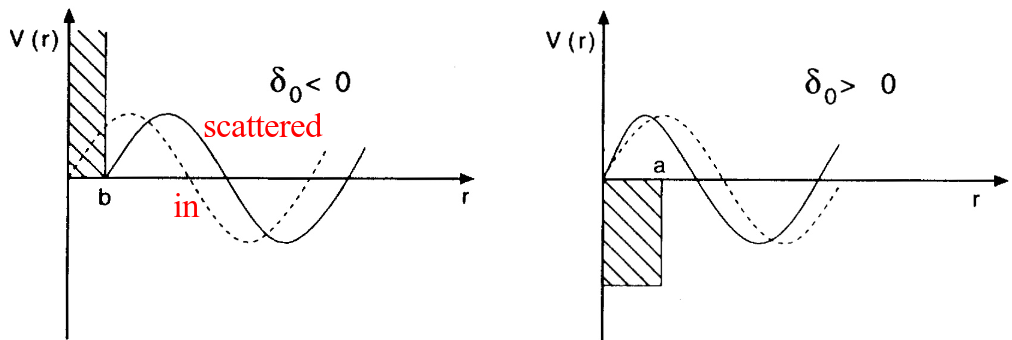
\includegraphics[width=0.7\linewidth]{fig-ch5/phase.png}}
  \caption{
  Examples of negative and positive phase shifts for repulsive and attractive potentials, respectively.
  }
\end{figure}
%\clearpage % flush figures 



The integrated cross section is given by
\[
\sigma = 2\pi \int_0^{\pi} |f(\theta)|^2 \sin \theta d\theta 
\]
\[
=2\pi \sum_l |\frac{(2l+1)}{k} \sin(\delta_l)|^2 \int_0^{\pi} (P_l(\cos(\theta)))^2 \sin(\theta) d\theta\]
\[ 
= \frac{4\pi}{k^2} \sum_l (2l+1) \sin^2\delta_l(k) = 4\pi \sum_l (2l+1)|f_l(\theta)|^2, 
\]
where the orthogonality of the Legendre polynomials was used to evaluate the last integral
\[
\int_0^{\pi} P_l(\cos \theta)^2 \sin \theta d\theta = \frac{2}{2l+1}.
\]
Thus, the \textbf{total} cross section is the sum of the partial-wave cross sections. Note that the differential cross section contains cross-terms from different partial waves. The integral over the full sphere enables the use of the legendre orthogonality, and this kills the cross-terms.




At low energy, $k \rightarrow 0$, S-waves are most important. In this region we can define the scattering length $a$ and the effective range $r$. The $S-$wave scattering amplitude is given by
\[
f_l(\theta) = \frac{1}{k}\frac{1}{\cot \delta_l(k) - i}.
\]
Taking the limit $k \rightarrow 0$, gives us the expansion
\[
k \cot \delta_0 = -\frac{1}{a} + \frac{1}{2}r_0 k^2 + \ldots
\]
Thus the low energy cross section is given by
\[
\sigma = 4\pi a^2.
\]
If the system contains a bound state, the scattering length will become positive (neutron-proton in $^3S_1$). For the $^1S_0$ wave, the scattering length is negative and large. This indicates that the wave function of the system is at the verge of turning over to get a node, but cannot create a bound state in this wave.




\begin{figure}[t]
  \centerline{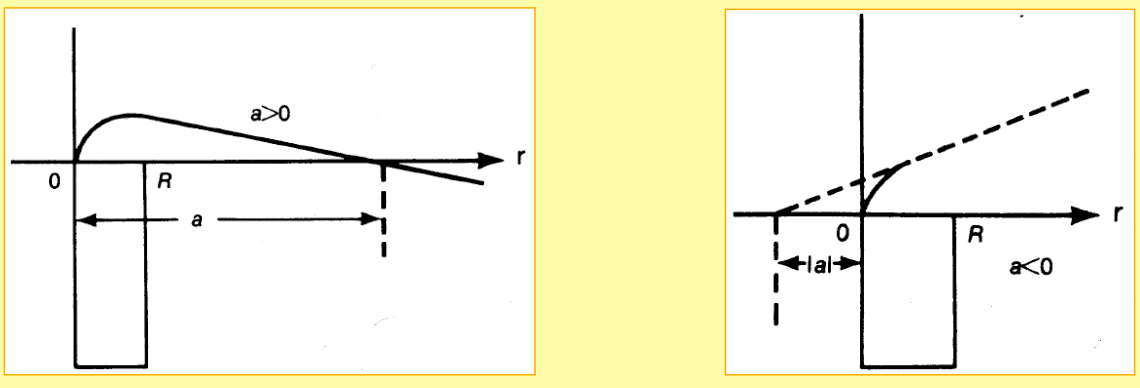
\includegraphics[width=1.0\linewidth]{fig-ch5/scattering_length.png}}
  \caption{
  Examples of scattering lengths.
  }
\end{figure}
%\clearpage % flush figures 



It is important to realize that the phase shifts themselves are not
observables. The measurable scattering quantity is the cross section,
or the differential cross section. The partial wave phase shifts can
be thought of as a parameterization of the (experimental) cross
sections. The phase shifts provide insights into the physics of
partial wave projected nuclear interactions, and are thus important
quantities to know.

The nucleon-nucleon differential cross section
have been measured at almost all energies up to the pion production
threshold (290 MeV in the Lab frame), and this experimental data base
is what provides us with the constraints on our nuclear interaction
models. In order to pin down the unknown coupling constants of the
theory, a statistical optimization with respect to cross sections need
to be carried out. This is how we constrain the nucleon-nucleon
interaction in practice!






\begin{figure}[t]
  \centerline{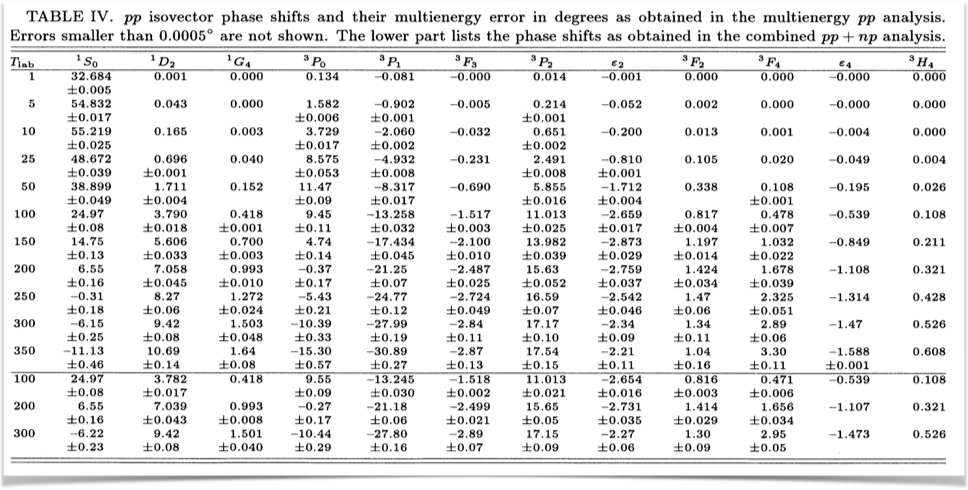
\includegraphics[width=1.0\linewidth]{fig-ch5/nijmegen_pp_phase_shifts.png}}
  \caption{
  Nijmegen phase shifts for selected partial waves.
  }
\end{figure}
%\clearpage % flush figures 


The $pp$-data is more accurate than the $np$-data, and for $nn$ there is no data. The quality of a potential is gauged by the $\chi^2$/datum with respect to the scattering data base





{\small   % Springer T2 style: small table font and more vspace

\vspace{4mm}

\begin{tabular}{ccccc}
\hline
\multicolumn{1}{c}{ $T_{\mathrm{lab}}$ bin (MeV) } & \multicolumn{1}{c}{ N3LO$^1$ } & \multicolumn{1}{c}{ NNLO$^2$ } & \multicolumn{1}{c}{ NLO$^2$ } & \multicolumn{1}{c}{ AV18$^3$ } \\
\hline
                             &                 &               &               &                 \\
0-100                        & 1.05            & 1.7           & 4.5           & 0.95            \\
100-190                      & 1.08            & 22            & 100           & 1.10            \\
190-290                      & 1.15            & 47            & 180           & 1.11            \\
$\mathbf{0-290}$             & $\mathbf{1.10}$ & $\mathbf{20}$ & $\mathbf{86}$ & $\mathbf{1.04}$ \\
\hline
\end{tabular}

\vspace{4mm}

}


\noindent
\begin{itemize}
\item R. Machleidt et al., Phys. Rev. C68, 041001(R) (2003)

\item E. Epelbaum et al., Eur. Phys. J. A19, 401 (2004)

\item R. B. Wiringa et al., Phys. Rev. C5, 38 (1995)
\end{itemize}

\noindent
An example: chiral twobody interactions
\[
\mathcal{L_{\mathrm{eff}}} = \mathcal{L}_{\pi \pi}(f_\pi,m_{\pi}) + \mathcal{L}_{\pi N}(f_{\pi},M_{N},g_A,c_i,d_i,...) + \mathcal{L}_{NN}(C_{i},\tilde{C}_{i},D_{i},...) + \ldots
\]
\begin{itemize}
\item R. Machleidt, D. R. Entem, Phys. Rep. 503, 1 (2011)

\item E. Epelbaum, H.-W. Hammer, Ulf-G. Mei\ss{}ner, Rev. Mod. Phys. 81, 1773 (2009)
\end{itemize}

\noindent
Proton-neutron $^1S_0$ phase shift
Note that the Nijm93 PWA phase shift becomes negative at T$_{\mathrm{lab}}> 250$MeV. This indicates that the nucleon-nucleon potential is repulsive at short distances 

\begin{figure}[t]
  \centerline{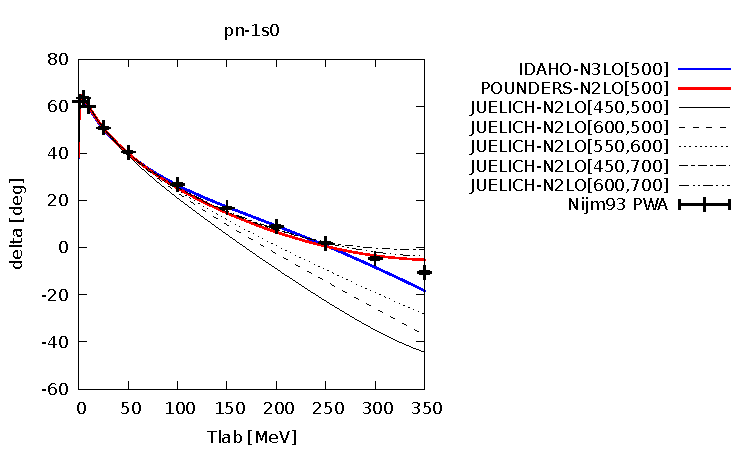
\includegraphics[width=0.7\linewidth]{fig-ch5/phase-pn-1s0_IDAHO_JUELICH.pdf}}
  \caption{
  Proton-neutron $^1S_0$ phase shift.
  }
\end{figure}
%\clearpage % flush figures 


 Differential cross section

\begin{figure}[t]
  \centerline{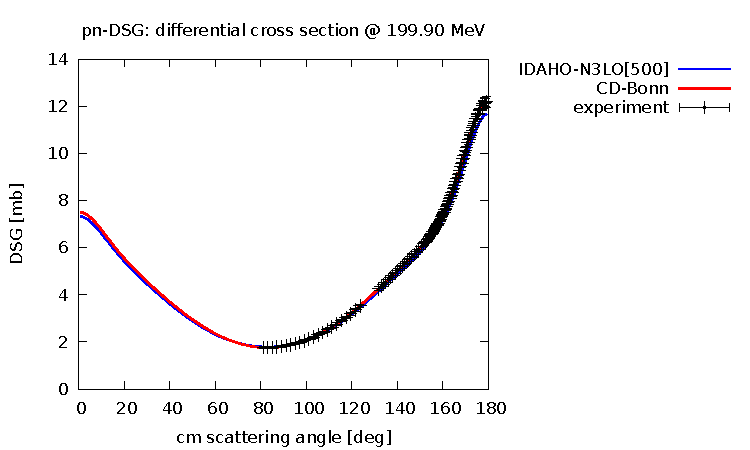
\includegraphics[width=0.8\linewidth]{fig-ch5/pnDSG_at_199MeV.pdf}}
  \caption{
  Proton-neutron $^1S_0$ phase shift.
  }
\end{figure}
%\clearpage % flush figures 








% --- begin exercise ---
\begin{doconceexercise}
\refstepcounter{doconceexercisecounter}

\subsection*{Exercise \thedoconceexercisecounter: Find all possible two-body quantum numbers}
\addcontentsline{loe}{doconceexercise}{Exercise \thedoconceexercisecounter: Find all possible two-body quantum numbers}


List all \textbf{allowed} according to the Pauli principle partial waves with isospin $T$, their 
projection $T_z$, spin $S$, orbital angular momentum $l$ and total spin $J$ for $J\le 3$.
Use the standard spectroscopic notation $^{2S+1}L_J$ to label different partial waves. A proton-proton state
has $T_Z=-1$, a proton-neutron state has $T_z=0$ and a neutron-neutron state has $T_z=1$.

\end{doconceexercise}
% --- end exercise ---




% --- begin exercise ---
\begin{doconceexercise}
\refstepcounter{doconceexercisecounter}

\subsection*{Exercise \thedoconceexercisecounter: Expressions for the various operators}
\addcontentsline{loe}{doconceexercise}{Exercise \thedoconceexercisecounter: Expressions for the various operators}



\subex{a)}
Find the closed form expression for the spin-orbit force. Show that the spin-orbit force {\bf LS} gives a zero
contribution for $S$-waves (orbital angular momentum $l=0$).   What is the value of the spin-orbit force for spin-singlet states ($S=0$)?

\subex{b)}
Find thereafter the expectation value of $\mathbf{\sigma}_1\cdot\mathbf{\sigma}_2$, where $\mathbf{\sigma}_i$ are so-called Pauli matrices. 
\begin{enumerate}
\item Add thereafter isospin and find the expectation value of $\mathbf{\sigma}_1\cdot\mathbf{\sigma}_2\mathbf{\tau}_1\cdot\mathbf{\tau}_2$, where $\mathbf{\tau}_i$ are also so-called Pauli matrices. List all the cases with $S=0,1$ and $T=0,1$.
\end{enumerate}

\noindent
\end{doconceexercise}
% --- end exercise ---




% --- begin exercise ---
\begin{doconceexercise}
\refstepcounter{doconceexercisecounter}

\subsection*{Exercise \thedoconceexercisecounter: One-pion exchange}
\addcontentsline{loe}{doconceexercise}{Exercise \thedoconceexercisecounter: One-pion exchange}


A simple parametrization of the nucleon-nucleon force is given by what is called the $V_8$ potential model,
where we have kept eight different operators. These operators contain a central force, a spin-orbit force,
a spin-spin force and a tensor force. Several features of the nuclei can be explained in terms of these four components. Without the Pauli matrices for isospin the final form of such an interaction model results in the following form: 
\[
V(\mathbf{r})= \left\{ C_c + C_\mathbf{\sigma} \mathbf{\sigma}_1\cdot\mathbf{\sigma}_2
 + C_T \left( 1 + {3\over m_\alpha r} + {3\over\left(m_\alpha r\right)^2}\right) S_{12} (\hat r)\right. 
\]
\[
\left. + C_{SL} \left( {1\over m_\alpha r} + {1\over \left( m_\alpha r\right)^2}
\right) \mathbf{L}\cdot \mathbf{S}
\right\} \frac{e^{-m_\alpha r}}{m_\alpha r}
\]
where $m_{\alpha}$ is the mass of the relevant meson and
$S_{12}$ is the familiar tensor term. The various coefficients $C_i$ are normally fitted so that the potential reproduces experimental scattering cross sections. By adding terms which include the isospin Pauli matrices 
results in an interaction model with eight operators.

The expectaction value of the tensor operator is non-zero only for $S=1$. We will show this in a forthcoming lecture, after that we have derived the Wigner-Eckart theorem. 
Here it suffices to know that the expectaction value of the tensor force for different partial values is  (with $l$ the orbital angular momentum and ${\cal J}$ the total angular momentum in the relative and center-of-mass frame of motion)
\[
\langle l {\cal J}S=1| S_{12} | l' {\cal J}S=1\rangle = -\frac{2{\cal J}({\cal J}+2)}{2{\cal J}+1} \hspace{0.5cm} l= {\cal J}+1 \hspace{0.1cm}\mathrm{and} \hspace{0.1cm} l'={\cal J}+1,
\]
\[
\langle l {\cal J}S=1| S_{12} | l' {\cal J}S=1\rangle = \frac{6\sqrt{{\cal J}({\cal J}+1)}}{2{\cal J}+1} \hspace{0.5cm} l= {\cal J}+1 \hspace{0.1cm}\mathrm{and} \hspace{0.1cm} l'={\cal J}-1,
\]
\[
\langle l {\cal J}S=1| S_{12} | l' {\cal J}S=1\rangle = \frac{6\sqrt{{\cal J}({\cal J}+1)}}{2{\cal J}+1} \hspace{0.5cm} l= {\cal J}-1 \hspace{0.1cm}\mathrm{and} \hspace{0.1cm} l'={\cal J}+1,
\]
\[
\langle l {\cal J}S=1| S_{12} | l' {\cal J}S=1\rangle = -\frac{2({\cal J}-1)}{2{\cal J}+1} \hspace{0.5cm} l= {\cal J}-1 \hspace{0.1cm}\mathrm{and} \hspace{0.1cm} l'={\cal J}-1,
\]
\[
\langle l {\cal J}S=1| S_{12} | l' {\cal J}S=1\rangle = 2 \hspace{0.5cm} l= {\cal J} \hspace{0.1cm}\mathrm{and} \hspace{0.1cm} l'={\cal J},
\]
and zero else.   

In this exercise we will focus only on the one-pion exchange term of the nuclear force, namely
\[
V_{\pi}(\mathbf{r})= -\frac{f_{\pi}^{2}}{4\pi m_{\pi}^{2}}\mathbf{ \tau}_1\cdot\mathbf{\tau}_2
\frac{1}{3}\left\{\mathbf{ \sigma}_1\cdot\mathbf{ \sigma}_2+\left( 1 + {3\over m_\pi r} + {3\over\left(m_\pi r\right)^2}\right) S_{12} (\hat r)\right\} \frac{e^{-m_\pi r}}{m_\pi r}.
\]
Here the constant $f_{\pi}^{2}/4\pi\approx 0.08$ and the mass of the pion is $m_\pi\approx 140$ MeV/c${}^{2}$.


\subex{a)}
Compute the expectation value of the tensor force and the spin-spin  and isospin operators for the one-pion exchange potential for all partial waves you found in exercise 9. Comment your results. How does the one-pion exchange part behave as function of different $l$, ${\cal J}$ and $S$ values? Do you see some patterns?

\subex{b)}
For the binding energy of the deuteron, with the ground state defined by the quantum numbers $l=0$, $S=1$ and ${\cal J}=1$, the tensor force plays an important role due to the admixture from the $l=2$ state. Use the expectation values of the different operators of the one-pion exchange potential and plot the ratio of the tensor force component over the spin-spin component of the one-pion exchange part as function of $x=m_\pi r$ for the $l=2$ state (that is the case $l,l'={\cal J}+1$). Comment your results.





\end{doconceexercise}
% --- end exercise ---


% !split
\chapter{Configuration interaction theory}
\label{ch:fci}

\section{Introduction}

The simplest possible choice for many-body wavefunctions are \textbf{product} wavefunctions.
That is
\[ 
\Psi(x_1, x_2, x_3, \ldots, x_A) \approx \phi_1(x_1) \phi_2(x_2) \phi_3(x_3) \ldots
\]
because we are really only good  at thinking about one particle at a time. Such 
product wavefunctions, without correlations, are easy to 
work with; for example, if the single-particle states $\phi_i(x)$ are orthonormal, then 
the product wavefunctions are easy to orthonormalize.   

Similarly, computing matrix elements of operators are relatively easy, because the 
integrals factorize.


The price we pay is the lack of correlations, which we must build up by using many, many product 
wavefunctions. (Thus we have a trade-off: compact representation of correlations but 
difficult integrals versus easy integrals but many states required.) 


Because we have fermions, we are required to have antisymmetric wavefunctions, e.g.
\[
\Psi(x_1, x_2, x_3, \ldots, x_A) = - \Psi(x_2, x_1, x_3, \ldots, x_A)
\]
etc. This is accomplished formally by using the determinantal formalism
\[
\Psi(x_1, x_2, \ldots, x_A) 
= \frac{1}{\sqrt{A!}} 
\det \left | 
\begin{array}{cccc}
\phi_1(x_1) & \phi_1(x_2) & \ldots & \phi_1(x_A) \\
\phi_2(x_1) & \phi_2(x_2) & \ldots & \phi_2(x_A) \\
 \vdots & & &  \\
\phi_A(x_1) & \phi_A(x_2) & \ldots & \phi_A(x_A) 
\end{array}
\right |
\]
Product wavefunction + antisymmetry = Slater determinant. 

\[
\Psi(x_1, x_2, \ldots, x_A) 
= \frac{1}{\sqrt{N!}} 
\det \left | 
\begin{array}{cccc}
\phi_1(x_1) & \phi_1(x_2) & \ldots & \phi_1(x_A) \\
\phi_2(x_1) & \phi_2(x_2) & \ldots & \phi_2(x_A) \\
 \vdots & & &  \\
\phi_A(x_1) & \phi_A(x_2) & \ldots & \phi_A(x_A) 
\end{array}
\right |
\]
Properties of the determinant (interchange of any two rows or 
any two columns yields a change in sign; thus no two rows and no 
two columns can be the same) lead to the Pauli principle:

\begin{itemize}
\item No two particles can be at the same place (two columns the same); and

\item No two particles can be in the same state (two rows the same).
\end{itemize}

\noindent
As a practical matter, however, Slater determinants beyond $N=4$ quickly become 
unwieldy. Thus we turn to the \textbf{occupation representation} or \textbf{second quantization} to simplify calculations. 

The occupation representation, using fermion \textbf{creation} and \textbf{annihilation} 
operators, is compact and efficient. It is also abstract and, at first encounter, not easy to 
internalize. It is inspired by other operator formalism, such as the ladder operators for 
the harmonic oscillator or for angular momentum, but unlike those cases, the operators \textbf{do not have coordinate space representations}.

Instead, one can think of fermion creation/annihilation operators as a game of symbols that 
compactly reproduces what one would do, albeit clumsily, with full coordinate-space Slater 
determinants. 


We start with a set of orthonormal single-particle states $\{ \phi_i(x) \}$. 
(Note: this requirement, and others, can be relaxed, but leads to a 
more involved formalism.) \textbf{Any} orthonormal set will do. 

To each single-particle state $\phi_i(x)$ we associate a creation operator 
$\hat{a}^\dagger_i$ and an annihilation operator $\hat{a}_i$. 

When acting on the vacuum state $| 0 \rangle$, the creation operator $\hat{a}^\dagger_i$ causes 
a particle to occupy the single-particle state $\phi_i(x)$:
\[
\phi_i(x) \rightarrow \hat{a}^\dagger_i |0 \rangle
\]


But with multiple creation operators we can occupy multiple states:
\[
\phi_i(x) \phi_j(x^\prime) \phi_k(x^{\prime \prime}) 
\rightarrow \hat{a}^\dagger_i \hat{a}^\dagger_j \hat{a}^\dagger_k |0 \rangle.
\]

Now we impose antisymmetry, by having the fermion operators satisfy  \textbf{anticommutation relations}:
\[
\hat{a}^\dagger_i \hat{a}^\dagger_j + \hat{a}^\dagger_j \hat{a}^\dagger_i
= [ \hat{a}^\dagger_i ,\hat{a}^\dagger_j ]_+ 
= \{ \hat{a}^\dagger_i ,\hat{a}^\dagger_j \} = 0
\]
so that 
\[
\hat{a}^\dagger_i \hat{a}^\dagger_j = - \hat{a}^\dagger_j \hat{a}^\dagger_i
\]


Because of this property, automatically $\hat{a}^\dagger_i \hat{a}^\dagger_i = 0$, 
enforcing the Pauli exclusion principle.  Thus when writing a Slater determinant 
using creation operators, 
\[
\hat{a}^\dagger_i \hat{a}^\dagger_j \hat{a}^\dagger_k \ldots |0 \rangle
\]
each index $i,j,k, \ldots$ must be unique.




\section{Full Configuration Interaction Theory}

We have defined the ansatz for the ground state as 
\[
|\Phi_0\rangle = \left(\prod_{i\le F}\hat{a}_{i}^{\dagger}\right)|0\rangle,
\]
where the index $i$ defines different single-particle states up to the Fermi level. We have assumed that we have $N$ fermions. 
A given one-particle-one-hole ($1p1h$) state can be written as
\[
|\Phi_i^a\rangle = \hat{a}_{a}^{\dagger}\hat{a}_i|\Phi_0\rangle,
\]
while a $2p2h$ state can be written as
\[
|\Phi_{ij}^{ab}\rangle = \hat{a}_{a}^{\dagger}\hat{a}_{b}^{\dagger}\hat{a}_j\hat{a}_i|\Phi_0\rangle,
\]
and a general $NpNh$ state as 
\[
|\Phi_{ijk\dots}^{abc\dots}\rangle = \hat{a}_{a}^{\dagger}\hat{a}_{b}^{\dagger}\hat{a}_{c}^{\dagger}\dots\hat{a}_k\hat{a}_j\hat{a}_i|\Phi_0\rangle.
\]


We can then expand our exact state function for the ground state 
as
\[
|\Psi_0\rangle=C_0|\Phi_0\rangle+\sum_{ai}C_i^a|\Phi_i^a\rangle+\sum_{abij}C_{ij}^{ab}|\Phi_{ij}^{ab}\rangle+\dots
=(C_0+\hat{C})|\Phi_0\rangle,
\]
where we have introduced the so-called correlation operator 
\[
\hat{C}=\sum_{ai}C_i^a\hat{a}_{a}^{\dagger}\hat{a}_i  +\sum_{abij}C_{ij}^{ab}\hat{a}_{a}^{\dagger}\hat{a}_{b}^{\dagger}\hat{a}_j\hat{a}_i+\dots
\]
Since the normalization of $\Psi_0$ is at our disposal and since $C_0$ is by hypothesis non-zero, we may arbitrarily set $C_0=1$ with 
corresponding proportional changes in all other coefficients. Using this so-called intermediate normalization we have
\[
\langle \Psi_0 | \Phi_0 \rangle = \langle \Phi_0 | \Phi_0 \rangle = 1, 
\]
resulting in 
\[
|\Psi_0\rangle=(1+\hat{C})|\Phi_0\rangle.
\]



We rewrite 
\[
|\Psi_0\rangle=C_0|\Phi_0\rangle+\sum_{ai}C_i^a|\Phi_i^a\rangle+\sum_{abij}C_{ij}^{ab}|\Phi_{ij}^{ab}\rangle+\dots,
\]
in a more compact form as 
\[
|\Psi_0\rangle=\sum_{PH}C_H^P\Phi_H^P=\left(\sum_{PH}C_H^P\hat{A}_H^P\right)|\Phi_0\rangle,
\]
where $H$ stands for $0,1,\dots,n$ hole states and $P$ for $0,1,\dots,n$ particle states. 
Our requirement of unit normalization gives
\[
\langle \Psi_0 | \Phi_0 \rangle = \sum_{PH}|C_H^P|^2= 1,
\]
and the energy can be written as 
\[
E= \langle \Psi_0 | \hat{H} |\Phi_0 \rangle= \sum_{PP'HH'}C_H^{*P}\langle \Phi_H^P | \hat{H} |\Phi_{H'}^{P'} \rangle C_{H'}^{P'}.
\]



\subsection{Full Configuration Interaction Theory}

Normally 
\[
E= \langle \Psi_0 | \hat{H} |\Phi_0 \rangle= \sum_{PP'HH'}C_H^{*P}\langle \Phi_H^P | \hat{H} |\Phi_{H'}^{P'} \rangle C_{H'}^{P'},
\]
is solved by diagonalization setting up the Hamiltonian matrix defined by the basis of all possible Slater determinants. A diagonalization
% to do: add text about Rayleigh-Ritz
is equivalent to finding the variational minimum   of 
\[
 \langle \Psi_0 | \hat{H} |\Phi_0 \rangle-\lambda \langle \Psi_0 |\Phi_0 \rangle,
\]
where $\lambda$ is a variational multiplier to be identified with the energy of the system.
The minimization process results in 
\[
\delta\left[ \langle \Psi_0 | \hat{H} |\Phi_0 \rangle-\lambda \langle \Psi_0 |\Phi_0 \rangle\right]=
\]
\[
\sum_{P'H'}\left\{\delta[C_H^{*P}]\langle \Phi_H^P | \hat{H} |\Phi_{H'}^{P'} \rangle C_{H'}^{P'}+
C_H^{*P}\langle \Phi_H^P | \hat{H} |\Phi_{H'}^{P'} \rangle \delta[C_{H'}^{P'}]-
\lambda( \delta[C_H^{*P}]C_{H'}^{P'}+C_H^{*P}\delta[C_{H'}^{P'}]\right\} = 0.
\]
Since the coefficients $\delta[C_H^{*P}]$ and $\delta[C_{H'}^{P'}]$ are complex conjugates it is necessary and sufficient to require the quantities that multiply with $\delta[C_H^{*P}]$ to vanish.  

This leads to 
\[
\sum_{P'H'}\langle \Phi_H^P | \hat{H} |\Phi_{H'}^{P'} \rangle C_{H'}^{P'}-\lambda C_H^{P}=0,
\]
for all sets of $P$ and $H$.

If we then multiply by the corresponding $C_H^{*P}$ and sum over $PH$ we obtain
\[ 
\sum_{PP'HH'}C_H^{*P}\langle \Phi_H^P | \hat{H} |\Phi_{H'}^{P'} \rangle C_{H'}^{P'}-\lambda\sum_{PH}|C_H^P|^2=0,
\]
leading to the identification $\lambda = E$. This means that we have for all $PH$ sets
\begin{equation}
\sum_{P'H'}\langle \Phi_H^P | \hat{H} -E|\Phi_{H'}^{P'} \rangle = 0. \label{eq:fullci}
\end{equation}


An alternative way to derive the last equation is to start from 
\[
(\hat{H} -E)|\Psi_0\rangle = (\hat{H} -E)\sum_{P'H'}C_{H'}^{P'}|\Phi_{H'}^{P'} \rangle=0, 
\]
and if this equation is successively projected against all $\Phi_H^P$ in the expansion of $\Psi$, then the last equation on the previous slide
results.   As stated previously, one solves this equation normally by diagonalization. If we are able to solve this equation exactly (that is
numerically exactly) in a large Hilbert space (it will be truncated in terms of the number of single-particle states included in the definition
of Slater determinants), it can then serve as a benchmark for other many-body methods which approximate the correlation operator
$\hat{C}$.  


For reasons to come (links with Coupled-Cluster theory and Many-Body perturbation theory), 
we will rewrite Eq.~(~\ref{eq:fullci}) as a set of coupled non-linear equations in terms of the unknown coefficients $C_H^P$. 

To see this, we look at the contributions arising from 
\[
\langle \Phi_H^P | = \langle \Phi_0|
\]
in  Eq.~(\ref{eq:fullci}), that is we multiply with $\langle \Phi_0 |$
from the left in 
\[
(\hat{H} -E)\sum_{P'H'}C_{H'}^{P'}|\Phi_{H'}^{P'} \rangle=0. 
\]
If we assume that we have a two-body operator at most, Slater's rule gives then an equation for the 
correlation energy in terms of $C_i^a$ and $C_{ij}^{ab}$ only.  We get then
\[
\langle \Phi_0 | \hat{H} -E| \Phi_0\rangle + \sum_{ai}\langle \Phi_0 | \hat{H} -E|\Phi_{i}^{a} \rangle C_{i}^{a}+
\sum_{abij}\langle \Phi_0 | \hat{H} -E|\Phi_{ij}^{ab} \rangle C_{ij}^{ab}=0,
\]
or 
\[
E-E_0 =\Delta E=\sum_{ai}\langle \Phi_0 | \hat{H}|\Phi_{i}^{a} \rangle C_{i}^{a}+
\sum_{abij}\langle \Phi_0 | \hat{H}|\Phi_{ij}^{ab} \rangle C_{ij}^{ab},
\]
where the energy $E_0$ is the reference energy and $\Delta E$ defines the so-called correlation energy.
The single-particle basis functions  could be the results of a Hartree-Fock calculation or just the eigenstates of the non-interacting part of the Hamiltonian. 

In our chapter on Hartree-Fock calculations, 
we have already computed the matrix $\langle \Phi_0 | \hat{H}|\Phi_{i}^{a}\rangle $ and $\langle \Phi_0 | \hat{H}|\Phi_{ij}^{ab}\rangle$.  If we are using a Hartree-Fock basis, then the matrix elements
$\langle \Phi_0 | \hat{H}|\Phi_{i}^{a}\rangle $ and we are left with a correlation energy given by
\[
E-E_0 =\Delta E^{HF}=\sum_{abij}\langle \Phi_0 | \hat{H}|\Phi_{ij}^{ab} \rangle C_{ij}^{ab}. 
\]


Inserting the various matrix elements we can rewrite the previous equation as
\[
\Delta E=\sum_{ai}\langle i| \hat{f}|a \rangle C_{i}^{a}+
\sum_{abij}\langle ij | \hat{v}| ab \rangle C_{ij}^{ab}.
\]
This equation determines the correlation energy but not the coefficients $C$. 
We need more equations. Our next step is to set up
\[
\langle \Phi_i^a | \hat{H} -E| \Phi_0\rangle + \sum_{bj}\langle \Phi_i^a | \hat{H} -E|\Phi_{j}^{b} \rangle C_{j}^{b}+
\sum_{bcjk}\langle \Phi_i^a | \hat{H} -E|\Phi_{jk}^{bc} \rangle C_{jk}^{bc}+
\sum_{bcdjkl}\langle \Phi_i^a | \hat{H} -E|\Phi_{jkl}^{bcd} \rangle C_{jkl}^{bcd}=0,
\]
as this equation will allow us to find an expression for the coefficents $C_i^a$ since we can rewrite this equation as 
\[
\langle i | \hat{f}| a\rangle +\langle \Phi_i^a | \hat{H}|\Phi_{i}^{a} \rangle C_{i}^{a}+ \sum_{bj\ne ai}\langle \Phi_i^a | \hat{H}|\Phi_{j}^{b} \rangle C_{j}^{b}+
\sum_{bcjk}\langle \Phi_i^a | \hat{H}|\Phi_{jk}^{bc} \rangle C_{jk}^{bc}+
\sum_{bcdjkl}\langle \Phi_i^a | \hat{H}|\Phi_{jkl}^{bcd} \rangle C_{jkl}^{bcd}=0.
\]


We rewrite this equation as
\[
C_{i}^{a}=-(\langle \Phi_i^a | \hat{H}|\Phi_{i}^{a})^{-1}
\]
\[
\times\left(\langle i | \hat{f}| a\rangle+ \sum_{bj\ne ai}\langle \Phi_i^a | \hat{H}|\Phi_{j}^{b} \rangle C_{j}^{b}+\sum_{bcjk}\langle \Phi_i^a | \hat{H}|\Phi_{jk}^{bc} \rangle C_{jk}^{bc}+
\sum_{bcdjkl}\langle \Phi_i^a | \hat{H}|\Phi_{jkl}^{bcd} \rangle C_{jkl}^{bcd}\right).
\]
Since these equations are solved iteratively ( that is we can start with a guess for the coefficients $C_i^a$), it is common to start the  iteration 
by setting 
\[
 C_{i}^{a}=-\frac{\langle i | \hat{f}| a\rangle}{\langle \Phi_i^a | \hat{H}|\Phi_{i}^{a}\rangle},
\]
and the denominator can be written as
\[
  C_{i}^{a}=\frac{\langle i | \hat{f}| a\rangle}{\langle i | \hat{f}| i\rangle-\langle a | \hat{f}| a\rangle+\langle ai | \hat{v}| ai\rangle}.
\]
The observant reader will however see that we need an equation for $C_{jk}^{bc}$ and $C_{jkl}^{bcd}$ as well.
To find equations for these coefficients we need then to continue our multiplications from the left with the various
$\Phi_{H}^P$ terms. 



For $C_{jk}^{bc}$ we need then
\[
\langle \Phi_{ij}^{ab} | \hat{H} -E| \Phi_0\rangle + \sum_{kc}\langle \Phi_{ij}^{ab} | \hat{H} -E|\Phi_{k}^{c} \rangle C_{k}^{c}+
\]
\[
\sum_{cdkl}\langle \Phi_{ij}^{ab} | \hat{H} -E|\Phi_{kl}^{cd} \rangle C_{kl}^{cd}+\sum_{cdeklm}\langle \Phi_{ij}^{ab} | \hat{H} -E|\Phi_{klm}^{cde} \rangle C_{klm}^{cde}+\sum_{cdefklmn}\langle \Phi_{ij}^{ab} | \hat{H} -E|\Phi_{klmn}^{cdef} \rangle C_{klmn}^{cdef}=0,
\]
and we can isolate the coefficients $C_{kl}^{cd}$ in a similar way as we did for the coefficients $C_{i}^{a}$. 
At the end we can rewrite our solution of the Schr\"odinger equation in terms of $n$ coupled equations for the coefficients $C_H^P$.
This is a very cumbersome way of solving the equation. However, by using this iterative scheme we can illustrate how we can compute the
various terms in the wave operator or correlation operator $\hat{C}$. We will later identify the calculation of the various terms $C_H^P$
as parts of different many-body approximations to full CI. In particular, ww can  relate this non-linear scheme with Coupled Cluster theory and
many-body perturbation theory. These theories will not be discussed in this course.


If we use a Hartree-Fock basis, we simplify this equation
\[
\Delta E=\sum_{ai}\langle i| \hat{f}|a \rangle C_{i}^{a}+
\sum_{abij}\langle ij | \hat{v}| ab \rangle C_{ij}^{ab}.
\]
What about
\[
\langle \Phi_i^a | \hat{H} -E| \Phi_0\rangle + \sum_{bj}\langle \Phi_i^a | \hat{H} -E|\Phi_{j}^{b} \rangle C_{j}^{b}+
\sum_{bcjk}\langle \Phi_i^a | \hat{H} -E|\Phi_{jk}^{bc} \rangle C_{jk}^{bc}+
\sum_{bcdjkl}\langle \Phi_i^a | \hat{H} -E|\Phi_{jkl}^{bcd} \rangle C_{jkl}^{bcd}=0,
\]
and
\[
\langle \Phi_{ij}^{ab} | \hat{H} -E| \Phi_0\rangle + \sum_{kc}\langle \Phi_{ij}^{ab} | \hat{H} -E|\Phi_{k}^{c} \rangle C_{k}^{c}+
\sum_{cdkl}\langle \Phi_{ij}^{ab} | \hat{H} -E|\Phi_{kl}^{cd} \rangle C_{kl}^{cd}+
\]
\[
\sum_{cdeklm}\langle \Phi_{ij}^{ab} | \hat{H} -E|\Phi_{klm}^{cde} \rangle C_{klm}^{cde}+\sum_{cdefklmn}\langle \Phi_{ij}^{ab} | \hat{H} -E|\Phi_{klmn}^{cdef} \rangle C_{klmn}^{cdef}=0?
\]







\section{Building a many-body basis}


In project 1 the plan  is to construct a working code that constructs the 
many-body Hamiltonian matrix in a basis of Slater determinants and to find the low-lying eigenenergies. 
This is referred to as the configuration-interaction method or shell-model diagonalization 
(or the interacting shell model). 

The first step in such codes--and in your project--is to construct the many-body basis.  

While the formalism is independent of the choice of basis, the \textbf{effectiveness} of a calculation 
will certainly be basis dependent. 

Furthermore there are common conventions useful to know.


First, the single-particle basis has angular momentum as a good quantum number.  You can 
imagine the single-particle wavefunctions being generated by a one-body Hamiltonian, 
for example a harmonic oscillator.  Modifications include harmonic oscillator plus 
spin-orbit splitting, or self-consistent mean-field potentials, or the Woods-Saxon potential which mocks 
up the self-consistent mean-field. 


For nuclei, the harmonic oscillator, modified by spin-orbit splitting, provides a useful language 
for describing single-particle states.


Each single-particle state is labeled by the following quantum numbers: 

\begin{itemize}
\item Orbital angular momentum $l$

\item Intrinsic spin $s$ = 1/2 for protons and neutrons

\item Angular momentum $j = l \pm 1/2$

\item $z$-component $j_z$ (or $m$)

\item Some labeling of the radial wavefunction, typically $n$ the number of nodes in  the radial wavefunction, but in the case of harmonic oscillator one can also use the principal quantum number $N$, where the harmonic oscillator energy is $(N+3/2)\hbar \omega$. 
\end{itemize}

\noindent
In this format one labels states by $n(l)_j$, with $(l)$ replaced by a letter:
$s$ for $l=0$, $p$ for $l=1$, $d$ for $l=2$, $f$ for $l=3$, and thenceforth alphabetical.


 In practice the single-particle space has to be severely truncated.  This truncation is 
typically based upon the single-particle energies, which is the effective energy 
from a mean-field potential. 

Sometimes we freeze the core and only consider a valence space. For example, one 
may assume a frozen ${}^{4}\mbox{He}$ core, with two protons and two neutrons in the $0s_{1/2}$ 
shell, and then only allow active particles in the $0p_{1/2}$ and $0p_{3/2}$ orbits. 


Another example is a frozen ${}^{16}\mbox{O}$ core, with eight protons and eight neutrons filling the 
$0s_{1/2}$,  $0p_{1/2}$ and $0p_{3/2}$ orbits, with valence particles in the 
$0d_{5/2}, 1s_{1/2}$ and $0d_{3/2}$ orbits.


Sometimes we refer to nuclei by the valence space where their last nucleons go.  
So, for example, we call ${}^{12}\mbox{C}$ a $p$-shell nucleus, while ${}^{26}\mbox{Al}$ is an 
$sd$-shell nucleus and ${}^{56}\mbox{Fe}$ is a $pf$-shell nucleus.



There are different kinds of truncations.

\begin{itemize}
\item For example, one can start with `filled' orbits (almost always the lowest), and then  allow one, two, three... particles excited out of those filled orbits. These are called  1p-1h, 2p-2h, 3p-3h excitations. 

\item Alternately, one can state a maximal orbit and allow all possible configurations with  particles occupying states up to that maximum. This is called \emph{full configuration}.

\item Finally, for particular use in nuclear physics, there is the \emph{energy} truncation, also  called the $N\hbar\Omega$ or $N_{max}$ truncation. 
\end{itemize}

\noindent
 Here one works in a harmonic oscillator basis, with each major oscillator shell assigned 
a principal quantum number $N=0,1,2,3,...$. 

The $N\hbar\Omega$ or $N_{max}$ truncation: Any configuration is given an noninteracting energy, which is the sum 
of the single-particle harmonic oscillator energies. (Thus this ignores 
spin-orbit splitting.)




Excited state are labeled relative to the lowest configuration by the 
number of harmonic oscillator quanta.

This truncation is useful because: if one includes \emph{all} configuration up to 
some $N_{max}$, and has a translationally invariant interaction, then the intrinsic 
motion and the center-of-mass motion factor. In other words, we can know exactly 
the center-of-mass wavefunction. 





In almost all cases, the many-body Hamiltonian is rotationally invariant. This means 
it commutes with the operators $\hat{J}^2, \hat{J}_z$ and so eigenstates will have 
good $J,M$. Furthermore, the eigenenergies do not depend upon the orientation $M$. 


Therefore we can choose to construct a many-body basis which has fixed $M$; this is 
called an $M$-scheme basis. 


Alternately, one can construct a many-body basis which has fixed $J$, or a $J$-scheme 
basis. 

The Hamiltonian matrix will have smaller dimensions (a factor of 10 or more)
 in the $J$-scheme than in the $M$-scheme. 
On the other hand, as we'll show in the next slide, the $M$-scheme is very easy to 
construct with Slater determinants, while the $J$-scheme basis states, and thus the 
matrix elements, are more complicated, almost always being linear combinations of 
$M$-scheme states. $J$-scheme bases are important and useful, but we'll focus on the 
simpler $M$-scheme.



The quantum number $m$ is additive (because the underlying group is Abelian): 
if a Slater determinant $\hat{a}_i^\dagger \hat{a}^\dagger_j \hat{a}^\dagger_k \ldots | 0 \rangle$ 
is built from single-particle states all with good $m$, then the total 
\[
M = m_i + m_j + m_k + \ldots
\]
This is \emph{not} true of $J$, because the angular momentum group SU(2) is not Abelian.

The upshot is that 
\begin{itemize}
\item It is easy to construct a Slater determinant with good total $M$;

\item It is trivial to calculate $M$ for each Slater determinant;

\item So it is easy to construct an $M$-scheme basis with fixed total $M$.
\end{itemize}

\noindent
Note that the individual $M$-scheme basis states will \emph{not}, in general, 
have good total $J$. 
Because the Hamiltonian is rotationally invariant, however, the eigenstates will 
have good $J$. (The situation is muddied when one has states of different $J$ that are 
nonetheless degenerate.) 


Example: two $j=1/2$ orbits



{\small   % Springer T2 style: small table font and more vspace

\vspace{4mm}

\begin{tabular}{ccccc}
\hline
\multicolumn{1}{c}{ Index } & \multicolumn{1}{c}{ $n$ } & \multicolumn{1}{c}{ $l$ } & \multicolumn{1}{c}{ $j$ } & \multicolumn{1}{c}{ $m_j$ } \\
\hline
1     & 0   & 0   & 1/2 & -1/2  \\
2     & 0   & 0   & 1/2 & 1/2   \\
3     & 1   & 0   & 1/2 & -1/2  \\
4     & 1   & 0   & 1/2 & 1/2   \\
\hline
\end{tabular}

\vspace{4mm}

}


\noindent
Note: the order is arbitrary.
There are $\left ( \begin{array}{c} 4 \\ 2 \end{array} \right) = 6$ two-particle states, 
which we list with the total $M$:



{\small   % Springer T2 style: small table font and more vspace

\vspace{4mm}

\begin{tabular}{cc}
\hline
\multicolumn{1}{c}{ Occupied } & \multicolumn{1}{c}{ $M$ } \\
\hline
1,2      & 0   \\
1,3      & -1  \\
1,4      & 0   \\
2,3      & 0   \\
2,4      & 1   \\
3,4      & 0   \\
\hline
\end{tabular}

\vspace{4mm}

}


\noindent
and 1 each with $M = \pm 1$.


Example: consider using only single particle states from the $0d_{5/2}$ space. 
They have the following quantum numbers



{\small   % Springer T2 style: small table font and more vspace

\vspace{4mm}

\begin{tabular}{ccccc}
\hline
\multicolumn{1}{c}{ Index } & \multicolumn{1}{c}{ $n$ } & \multicolumn{1}{c}{ $l$ } & \multicolumn{1}{c}{ $j$ } & \multicolumn{1}{c}{ $m_j$ } \\
\hline
1     & 0   & 2   & 5/2 & -5/2  \\
2     & 0   & 2   & 5/2 & -3/2  \\
3     & 0   & 2   & 5/2 & -1/2  \\
4     & 0   & 2   & 5/2 & 1/2   \\
5     & 0   & 2   & 5/2 & 3/2   \\
6     & 0   & 2   & 5/2 & 5/2   \\
\hline
\end{tabular}

\vspace{4mm}

}


\noindent
There are $\left ( \begin{array}{c} 6 \\ 2 \end{array} \right) = 15$ two-particle states, 
which we list with the total $M$:



{\small   % Springer T2 style: small table font and more vspace

\vspace{4mm}

\begin{tabular}{cccccc}
\hline
\multicolumn{1}{c}{ Occupied } & \multicolumn{1}{c}{ $M$ } & \multicolumn{1}{c}{ Occupied } & \multicolumn{1}{c}{ $M$ } & \multicolumn{1}{c}{ Occupied } & \multicolumn{1}{c}{ $M$ } \\
\hline
1,2      & -4  & 2,3      & -2  & 3,5      & 1   \\
1,3      & -3  & 2,4      & -1  & 3,6      & 2   \\
1,4      & -2  & 2,5      & 0   & 4,5      & 2   \\
1,5      & -1  & 2,6      & 1   & 4,6      & 3   \\
1,6      & 0   & 3,4      & 0   & 5,6      & 4   \\
\hline
\end{tabular}

\vspace{4mm}

}


\noindent

\subsection{Basic steps in a building an FCI code}

The basic goal of the project is for you to build your own configuration-interaction  shell-model 
code. The code will be fairly basic; it will assume that we have 
a single species of particles, e.g.~only neutrons, 
and you could, if you wish to,  read in uncoupled two-body matrix elements.  Furthermore the pieces of the code will not 
be the most efficient.  Nonetheless it will be usable; most importantly, you will gain a good idea of what goes into a many-body shell-model code.

The first step  is to construct the $M$-scheme basis of Slater determinants.
Here $M$-scheme means the total $J_z$ of the many-body states is fixed.

The steps could be:

\begin{itemize}
\item Read in a user-supplied file of single-particle states (examples can be given) or just code these internally;

\item Ask for the total $M$ of the system and the number of particles $N$;

\item Construct all the $N$-particle states with given $M$.  You will validate the code by  comparing both the number of states and specific states.
\end{itemize}

\noindent
The format of a possible input  file could be


{\small   % Springer T2 style: small table font and more vspace

\vspace{4mm}

\begin{tabular}{ccccc}
\hline
\multicolumn{1}{c}{ Index } & \multicolumn{1}{c}{ $n$ } & \multicolumn{1}{c}{ $l$ } & \multicolumn{1}{c}{ $2j$ } & \multicolumn{1}{c}{ $2m_j$ } \\
\hline
1     & 1   & 0   & 1    & -1     \\
2     & 1   & 0   & 1    & 1      \\
3     & 0   & 2   & 3    & -3     \\
4     & 0   & 2   & 3    & -1     \\
5     & 0   & 2   & 3    & 1      \\
6     & 0   & 2   & 3    & 3      \\
7     & 0   & 2   & 5    & -5     \\
8     & 0   & 2   & 5    & -3     \\
9     & 0   & 2   & 5    & -1     \\
10    & 0   & 2   & 5    & 1      \\
11    & 0   & 2   & 5    & 3      \\
12    & 0   & 2   & 5    & 5      \\
\hline
\end{tabular}

\vspace{4mm}

}


\noindent
This represents the $1s_{1/2}0d_{3/2}0d_{5/2}$ valence space, or just the $sd$-space.  There are 
twelve single-particle states, labeled by an overall index, and which have associated quantum 
numbers the number of radial nodes, the orbital angular momentum $l$, and the 
angular momentum $j$ and third component $j_z$.  To keep everything as integers, we could store $2 \times j$ and 
$2 \times j_z$. 


To read in the single-particle states you need to:
\begin{itemize}
\item Open the file 
\begin{itemize}

 \item Read the number of single-particle states (in the above example, 12);  allocate memory; all you need is a single array storing $2\times j_z$ for each state, labeled by the index.

\end{itemize}

\noindent
\item Read in the quantum numbers and store $2 \times j_z$ (and anything else you happen to want).
\end{itemize}

\noindent
The next step is to read in the number of particles $N$ and the fixed total $M$ (or, actually, $2 \times M$). 
For this project we assume only a single species of particles, say neutrons, although this can be 
relaxed. \textbf{Note}: Although it is often a good idea to try to write a more general code, given the 
short time alloted we would suggest you keep your ambition in check, at least in the initial phases of the 
project.  


You should probably write an error trap to make sure $N$ and $M$ are congruent; if $N$ is even, then 
$2 \times M$ should be even, and if $N$ is odd then $2\times M$ should be odd. 


The final step is to generate the set of $N$-particle Slater determinants with fixed $M$. 
The Slater determinants will be stored in occupation representation.  Although in many codes
this representation is done compactly in bit notation with ones and zeros, but for 
greater transparency and simplicity we will list the occupied single particle states.

 Hence we can 
store the Slater determinant basis states as $sd(i,j)$, that is an 
array of dimension $N_{SD}$, the number of Slater determinants, by $N$, the number of occupied 
state. So if for the 7th Slater determinant the 2nd, 3rd, and 9th single-particle states are occupied, 
then $sd(7,1) = 2$, $sd(7,2) = 3$, and $sd(7,3) = 9$.


We can construct an occupation representation of Slater determinants by the \emph{odometer}
method.  Consider $N_{sp} = 12$ and $N=4$. 
Start with the first 4 states occupied, that is:

\begin{itemize}
\item $sd(1,:)= 1,2,3,4$ (also written as $|1,2,3,4 \rangle$)
\end{itemize}

\noindent
Now increase the last occupancy recursively:
\begin{itemize}
\item $sd(2,:)= 1,2,3,5$

\item $sd(3,:)= 1,2,3,6$

\item $sd(4,:)= 1,2,3,7$

\item $\ldots$

\item $sd(9,:)= 1,2,3,12$
\end{itemize}

\noindent
Then start over with 
\begin{itemize}
\item $sd(10,:)= 1,2,4,5$
\end{itemize}

\noindent
and again increase the rightmost digit

\begin{itemize}
\item $sd(11,:)= 1,2,4,6$

\item $sd(12,:)= 1,2,4,7$

\item $\ldots$

\item $sd(17,:)= 1,2,4,12$
\end{itemize}

\noindent
When we restrict ourselves to an $M$-scheme basis, we could choose two paths. 
The first is simplest (and simplest is often best, at 
least in the first draft of a code): generate all possible Slater determinants, 
and then extract from this initial list a list of those Slater determinants with a given 
$M$. (You will need to write a short function or routine that computes $M$ for any 
given occupation.)  


Alternately, and not too difficult, is to run the odometer routine twice: each time, as 
as a Slater determinant is calculated, compute $M$, but do not store the Slater determinants 
except the current one. You can then count up the number of Slater determinants with a 
chosen $M$.  Then allocated storage for the Slater determinants, and run the odometer 
algorithm again, this time storing Slater determinants with the desired $M$ (this can be 
done with a simple logical flag). 



\emph{Some example solutions}:  Let's begin with a simple case, the $0d_{5/2}$ space containing six single-particle states



{\small   % Springer T2 style: small table font and more vspace

\vspace{4mm}

\begin{tabular}{ccccc}
\hline
\multicolumn{1}{c}{ Index } & \multicolumn{1}{c}{ $n$ } & \multicolumn{1}{c}{ $l$ } & \multicolumn{1}{c}{ $j$ } & \multicolumn{1}{c}{ $m_j$ } \\
\hline
1     & 0   & 2   & 5/2 & -5/2  \\
2     & 0   & 2   & 5/2 & -3/2  \\
3     & 0   & 2   & 5/2 & -1/2  \\
4     & 0   & 2   & 5/2 & 1/2   \\
5     & 0   & 2   & 5/2 & 3/2   \\
6     & 0   & 2   & 5/2 & 5/2   \\
\hline
\end{tabular}

\vspace{4mm}

}


\noindent
For two particles, there are a total of 15 states, which we list here with the total $M$:
\begin{itemize}
\item $| 1,2 \rangle$, $M= -4$,  $| 1,3 \rangle$, $M= -3$

\item $| 1,4 \rangle$, $M= -2$, $| 1,5 \rangle$, $M= -1$

\item $| 1,5 \rangle$, $M= 0$, $| 2,3 \rangle$, $M= -2$

\item $| 2,4 \rangle$, $M= -1$, $| 2,5 \rangle$, $M= 0$

\item $| 2,6 \rangle$, $M= 1$, $| 3,4 \rangle$, $M= 0$

\item $| 3,5 \rangle$, $M= 1$, $| 3,6 \rangle$, $M= 2$

\item $| 4,5 \rangle$, $M= 2$, $ | 4,6 \rangle$, $M= 3$

\item $| 5,6 \rangle$, $M= 4$
\end{itemize}

\noindent
Of these, there are only 3 states with $M=0$. 

\emph{You should try} by hand to show that in this same single-particle space, that for 
$N=3$ there are 3 states with $M=1/2$ and for $N= 4$ there are also only 3 states with $M=0$. 

\emph{To test your code}, confirm the above. 

Also, 
for the $sd$-space given above, for $N=2$ there are 14 states with $M=0$, for $N=3$ there are 37 
states with $M=1/2$, for $N=4$ there are 81 states with $M=0$.


For our project, we will only consider the pairing model.
A simple space is the $(1/2)^2$ space with four single-particle states



{\small   % Springer T2 style: small table font and more vspace

\vspace{4mm}

\begin{tabular}{ccccc}
\hline
\multicolumn{1}{c}{ Index } & \multicolumn{1}{c}{ $n$ } & \multicolumn{1}{c}{ $l$ } & \multicolumn{1}{c}{ $s$ } & \multicolumn{1}{c}{ $m_s$ } \\
\hline
1     & 0   & 0   & 1/2 & -1/2  \\
2     & 0   & 0   & 1/2 & 1/2   \\
3     & 1   & 0   & 1/2 & -1/2  \\
4     & 1   & 0   & 1/2 & 1/2   \\
\hline
\end{tabular}

\vspace{4mm}

}


\noindent
For $N=2$ there are 4 states with $M=0$; show this by hand and confirm your code reproduces it. 


Another, slightly more challenging space is the $(1/2)^4$ space, that is, 
with eight  single-particle states we have



{\small   % Springer T2 style: small table font and more vspace

\vspace{4mm}

\begin{tabular}{ccccc}
\hline
\multicolumn{1}{c}{ Index } & \multicolumn{1}{c}{ $n$ } & \multicolumn{1}{c}{ $l$ } & \multicolumn{1}{c}{ $s$ } & \multicolumn{1}{c}{ $m_s$ } \\
\hline
1     & 0   & 0   & 1/2 & -1/2  \\
2     & 0   & 0   & 1/2 & 1/2   \\
3     & 1   & 0   & 1/2 & -1/2  \\
4     & 1   & 0   & 1/2 & 1/2   \\
5     & 2   & 0   & 1/2 & -1/2  \\
6     & 2   & 0   & 1/2 & 1/2   \\
7     & 3   & 0   & 1/2 & -1/2  \\
8     & 3   & 0   & 1/2 & 1/2   \\
\hline
\end{tabular}

\vspace{4mm}

}


\noindent
For $N=2$ there are 16 states with $M=0$; for $N=3$ there are 24 states with $M=1/2$, and for 
$N=4$ there are 36 states with $M=0$. 


In the shell-model context we can interpret this as 4 $s_{1/2}$ levels, with $m = \pm 1/2$, we can also think of these are simple four pairs,  $\pm k, k = 1,2,3,4$. Later on we will 
assign single-particle energies,  depending on the radial quantum number $n$, that is, 
$\epsilon_k = |k| \delta$ so that they are equally spaced.


For application in the pairing model we can go further and consider only states with 
no ``broken pairs,'' that is, if $+k$ is filled (or $m = +1/2$, so is $-k$ ($m=-1/2$). 
If you want, you can write your code to accept only these, and obtain the following 
six states:

\begin{itemize}
\item $|           1,           2 ,          3         ,       4  \rangle , $

\item $|            1      ,     2        ,        5         ,       6 \rangle , $

\item $|            1         ,       2     ,           7         ,       8  \rangle , $

\item $|            3        ,        4      ,          5          ,      6  \rangle , $

\item $|            3        ,        4      ,          7         ,       8  \rangle , $

\item $|            5        ,        6     ,           7     ,           8  \rangle $

\item Write small modules (routines/functions) ; avoid big functions  that do everything. (But not too small.)

\item Write lots of error traps, even for things that are `obvious.'

\item Document as you go along.  For each function write a header that includes: 
\begin{enumerate}

\item Main purpose of function

\item names and  brief explanation of input variables, if any 

\item names and brief explanation of output variables, if any

\item functions called by this function

\item called by which functions
\end{enumerate}

\noindent
\end{itemize}

\noindent
Hints for coding

\begin{itemize}
\item When debugging, print out intermediate values. It's almost impossible to debug a  code by looking at it--the code will almost always win a `staring contest.'

\item Validate code with SIMPLE CASES. Validate early and often.   
\end{itemize}

\noindent
The number one mistake is using a too complex a system to test. For example ,
if you are computing particles in a potential in a box, try removing the potential--you should get 
particles in a box. And start with one particle, then two, then three... Don't start with 
eight particles.


Our recommended occupation representation, e.g.~$| 1,2,4,8 \rangle$, is 
easy to code, but numerically inefficient when one has hundreds of 
millions of Slater determinants.


In state-of-the-art shell-model codes, one generally uses bit 
representation, i.e.~$|1101000100... \rangle$ where one stores 
the Slater determinant as a single (or a small number of) integer.


This is much more compact, but more intricate to code with considerable 
more overhead. There exist 
bit-manipulation functions. 
This is left as a challenge for those of you who would like to study this topic further for the final project to be presented for the oral examination.


\subsection{Example case: pairing Hamiltonian}

We consider a space with $2\Omega$ single-particle states, with each 
state labeled by 
$k = 1, 2, 3, \Omega$ and $m = \pm 1/2$. The convention is that 
the state with $k>0$ has $m = + 1/2$ while $-k$ has $m = -1/2$.


The Hamiltonian we consider is 
\[
\hat{H} = -G \hat{P}_+ \hat{P}_-,
\]
where
\[
\hat{P}_+ = \sum_{k > 0} \hat{a}^\dagger_k \hat{a}^\dagger_{-{k}}.
\]
and $\hat{P}_- = ( \hat{P}_+)^\dagger$.

This problem can be solved using what is called the quasi-spin formalism to obtain the 
exact results. Thereafter we will try again using the explicit Slater determinant formalism.


One can show (and this is part of the project) that
\[
\left [ \hat{P}_+, \hat{P}_- \right ] = \sum_{k> 0} \left( \hat{a}^\dagger_k \hat{a}_k 
+ \hat{a}^\dagger_{-{k}} \hat{a}_{-{k}} - 1 \right) = \hat{N} - \Omega.
\]
Now define 
\[
\hat{P}_z = \frac{1}{2} ( \hat{N} -\Omega).
\]
Finally you can show
\[
\left [ \hat{P}_z , \hat{P}_\pm \right ] = \pm \hat{P}_\pm.
\]
This means the operators $\hat{P}_\pm, \hat{P}_z$ form a so-called  $SU(2)$ algebra, and we can 
use all our insights about angular momentum, even though there is no actual 
angular momentum involved (this is similar to project 1).

So we rewrite the Hamiltonian to make this explicit:
\[
\hat{H} = -G \hat{P}_+ \hat{P}_- 
= -G \left( \hat{P}^2 - \hat{P}_z^2 + \hat{P}_z\right)
\]


Because of the SU(2) algebra, we know that the eigenvalues of 
$\hat{P}^2$ must be of the form $p(p+1)$, with $p$ either integer or half-integer, and the eigenvalues of $\hat{P}_z$ 
are $m_p$ with $p \geq | m_p|$, with $m_p$ also integer or half-integer. 


But because $\hat{P}_z = (1/2)(\hat{N}-\Omega)$, we know that for $N$ particles 
the value $m_p = (N-\Omega)/2$. Furthermore, the values of $m_p$ range from 
$-\Omega/2$ (for $N=0$) to $+\Omega/2$ (for $N=2\Omega$, with all states filled). 

We deduce the maximal $p = \Omega/2$ and for a given $n$ the 
values range of $p$ range from $|N-\Omega|/2$ to $\Omega/2$ in steps of 1 
(for an even number of particles) 


Following Racah we introduce the notation
$p = (\Omega - v)/2$
where $v = 0, 2, 4,..., \Omega - |N-\Omega|$ 
With this it is easy to deduce that the eigenvalues of the pairing Hamiltonian are
\[
-G(N-v)(2\Omega +2-N-v)/4
\]
This also works for $N$ odd, with $v= 1,3,5, \dots$.



Let's take a specific example: $\Omega = 3$ so there are 6 single-particle states, 
and $N = 3$, with $v= 1,3$. Therefore there are two distinct eigenvalues, 
\[
E = -2G, 0
\]
Now let's work this out explicitly. The single particle degrees of freedom are defined as



{\small   % Springer T2 style: small table font and more vspace

\vspace{4mm}

\begin{tabular}{ccc}
\hline
\multicolumn{1}{c}{ Index } & \multicolumn{1}{c}{ $k$ } & \multicolumn{1}{c}{ $m$ } \\
\hline
1     & 1   & -1/2 \\
2     & -1  & 1/2  \\
3     & 2   & -1/2 \\
4     & -2  & 1/2  \\
5     & 3   & -1/2 \\
6     & -3  & 1/2  \\
\hline
\end{tabular}

\vspace{4mm}

}


\noindent
 There are  $\left( \begin{array}{c}6 \\ 3 \end{array} \right) = 20$ three-particle states, but there 
are 9 states with $M = +1/2$, namely
$| 1,2,3 \rangle, |1,2,5\rangle, | 1,4,6 \rangle, | 2,3,4 \rangle, |2,3,6 \rangle, | 2,4,5 \rangle, | 2, 5, 6 \rangle, |3,4,6 \rangle, | 4,5,6 \rangle$.











In this basis, the operator 
\[
\hat{P}_+
= \hat{a}^\dagger_1 \hat{a}^\dagger_2 + \hat{a}^\dagger_3 \hat{a}^\dagger_4 +
\hat{a}^\dagger_5 \hat{a}^\dagger_6 
\]
From this we can determine that 
\[
\hat{P}_- | 1, 4, 6 \rangle = \hat{P}_- | 2, 3, 6 \rangle
= \hat{P}_- | 2, 4, 5 \rangle = 0
\]
so those states all have eigenvalue 0.


Now for further example, 
\[
\hat{P}_- | 1,2,3 \rangle = | 3 \rangle
\]
so
\[
\hat{P}_+ \hat{P}_- | 1,2,3\rangle = | 1,2,3\rangle+ | 3,4,3\rangle + | 5,6,3\rangle
\]
The second term vanishes because state 3 is occupied twice, and reordering the last 
term we
get
\[
\hat{P}_+ \hat{P}_- | 1,2,3\rangle = | 1,2,3\rangle+ |3, 5,6\rangle
\]
without picking up a phase.



Continuing in this fashion, with the previous ordering of the many-body states
(  $| 1,2,3 \rangle, |1,2,5\rangle, | 1,4,6 \rangle, | 2,3,4 \rangle, |2,3,6 \rangle, | 2,4,5 \rangle, | 2, 5, 6 \rangle, |3,4,6 \rangle, | 4,5,6 \rangle$) the 
Hamiltonian matrix of this system is 
\[
H = -G\left( 
\begin{array}{ccccccccc}
1 & 0 & 0 & 0 & 0 & 0 & 0 & 0 & 1  \\
0 & 1 & 0 & 0 & 0 & 0 & 0 & 1 & 0  \\
0 & 0 & 0 & 0 & 0 & 0 & 0 & 0 & 0  \\
0 & 0 & 0 & 1 & 0 & 0 & 1 & 0 & 0  \\
0 & 0 & 0 & 0 & 0 & 0 & 0 & 0 & 0  \\
0 & 0 & 0 & 0 & 0 & 0 & 0 & 0 & 0  \\
0 & 0 & 0 & 1 & 0 & 0 & 1 & 0 & 0  \\
0 & 0 & 0 & 0 & 0 & 0 & 0 & 0 & 0  \\
0 & 1 & 0 & 0 & 0 & 0 & 0 & 1 & 0  \\
1 & 0 & 0 & 0 & 0 & 0 & 0 & 0 & 1  
\end{array} \right )
\] 
This is useful for our project.  One can by hand confirm 
that there are 3 eigenvalues $-2G$ and 6 with value zero.



Another example
Using the $(1/2)^4$ single-particle space, resulting in eight single-particle states



{\small   % Springer T2 style: small table font and more vspace

\vspace{4mm}

\begin{tabular}{ccccc}
\hline
\multicolumn{1}{c}{ Index } & \multicolumn{1}{c}{ $n$ } & \multicolumn{1}{c}{ $l$ } & \multicolumn{1}{c}{ $s$ } & \multicolumn{1}{c}{ $m_s$ } \\
\hline
1     & 0   & 0   & 1/2 & -1/2  \\
2     & 0   & 0   & 1/2 & 1/2   \\
3     & 1   & 0   & 1/2 & -1/2  \\
4     & 1   & 0   & 1/2 & 1/2   \\
5     & 2   & 0   & 1/2 & -1/2  \\
6     & 2   & 0   & 1/2 & 1/2   \\
7     & 3   & 0   & 1/2 & -1/2  \\
8     & 3   & 0   & 1/2 & 1/2   \\
\hline
\end{tabular}

\vspace{4mm}

}


\noindent
and then taking only 4-particle, $M=0$ states that have no `broken pairs', there are six basis Slater 
determinants:

\begin{itemize}
\item $|           1,           2 ,          3         ,       4  \rangle , $

\item $|            1      ,     2        ,        5         ,       6 \rangle , $

\item $|            1         ,       2     ,           7         ,       8  \rangle , $

\item $|            3        ,        4      ,          5          ,      6  \rangle , $

\item $|            3        ,        4      ,          7         ,       8  \rangle , $

\item $|            5        ,        6     ,           7     ,           8  \rangle $
\end{itemize}

\noindent
Now we take the following Hamiltonian
\[
\hat{H} = \sum_n n \delta \hat{N}_n  - G \hat{P}^\dagger \hat{P}
\]
where 
\[
\hat{N}_n = \hat{a}^\dagger_{n, m=+1/2} \hat{a}_{n, m=+1/2} +
\hat{a}^\dagger_{n, m=-1/2} \hat{a}_{n, m=-1/2}
\]
and
\[
\hat{P}^\dagger = \sum_{n} \hat{a}^\dagger_{n, m=+1/2} \hat{a}^\dagger_{n, m=-1/2} 
\]
We can write down the $ 6 \times 6$  Hamiltonian in the basis from the prior slide:
\[
H = \left ( 
\begin{array}{cccccc}
2\delta -2G & -G & -G & -G & -G & 0 \\
 -G & 4\delta -2G & -G & -G & -0 & -G \\
-G & -G & 6\delta -2G & 0 & -G & -G \\
 -G & -G & 0 & 6\delta-2G & -G & -G \\
 -G & 0 & -G & -G & 8\delta-2G & -G \\
0 & -G & -G & -G & -G & 10\delta -2G 
\end{array} \right )
\]
(You should check by hand that this is correct.) 

For $\delta = 0$ we have the closed form solution of  the g.s. energy given by $-6G$.










\subsection{Angular momentum algebra, Wigner-Eckart theorem}

\begin{itemize}
\item We need to define the so-called $6j$ and $9j$ symbols

\item The Wigner-Eckart theorem

\item We will also study  some specific examples, like the calculation of the tensor force.
\end{itemize}

\noindent
We define an irreducible  spherical tensor $T^{\lambda}_{\mu}$ of rank $\lambda$ as an operator with $2\lambda+1$ components $\mu$ 
that satisfies the commutation relations ($\hbar=1$)
\[
[J_{\pm}, T^{\lambda}_{\mu}]= \sqrt{(\lambda\mp \mu)(\lambda\pm \mu+1)}T^{\lambda}_{\mu\pm 1},
\]
and
\[
[J_{z}, T^{\lambda}_{\mu}]=\mu T^{\lambda}_{\mu}.
\]

Our angular momentum coupled two-body wave function obeys clearly this definition, namely
\[
|(ab)JM\rangle  = \left\{a^{\dagger}_aa^{\dagger}_b\right\}^J_M|\Phi_0\rangle=N_{ab}\sum_{m_am_b}\langle j_am_aj_bm_b|JM\rangle|\Phi^{ab}\rangle, 
\]
is a tensor of rank $J$ with $M$ components. Another well-known example is given by the spherical harmonics (see examples during today's lecture). 

The product of two irreducible tensor operators
\[
T^{\lambda_3}_{\mu_3}=\sum_{\mu_1\mu_2}\langle \lambda_1\mu_1\lambda_2\mu_2|\lambda_3\mu_3\rangle T^{\lambda_1}_{\mu_1}T^{\lambda_2}_{\mu_2}
\] 
is also a tensor operator of rank $\lambda_3$. 


We wish to apply the above definitions to the computations of a matrix element
\[
\langle \Phi^J_M|T^{\lambda}_{\mu}|\Phi^{J'}_{M'}\rangle,
\]
where we have skipped a reference to specific single-particle states. This is the expectation value for two specific states, labelled by angular momenta $J'$ and $J$. These states form an orthonormal basis.
Using the properties of the Clebsch-Gordan coefficients we can write 
\[
T^{\lambda}_{\mu}|\Phi^{J'}_{M'}\rangle=\sum_{J''M''}\langle \lambda \mu J'M'|J''M''\rangle|\Psi^{J''}_{M''}\rangle,
\]
and assuming that states with different $J$ and $M$ are orthonormal we arrive at
\[
\langle \Phi^J_M|T^{\lambda}_{\mu}|\Phi^{J'}_{M'}\rangle= \langle \lambda \mu J'M'|JM\rangle \langle \Phi^J_M|\Psi^{J}_{M}\rangle.
\]

We need to show that 
\[
\langle \Phi^J_M|\Psi^{J}_{M}\rangle,
\]
is independent of $M$.
To show that 
\[
\langle \Phi^J_M|\Psi^{J}_{M}\rangle,
\]
is independent of $M$, we use the ladder operators for angular momentum.


 We have that
\[
\langle \Phi^J_{M+1}|\Psi^{J}_{M+1}\rangle=\left((J-M)(J+M+1)\right)^{-1/2}\langle \hat{J}_{+}\Phi^J_{M}|\Psi^{J}_{M+1}\rangle,
\]
but this is also equal to 
\[
\langle \Phi^J_{M+1}|\Psi^{J}_{M+1}\rangle=\left((J-M)(J+M+1)\right)^{-1/2}\langle \Phi^J_{M}|\hat{J}_{-}\Psi^{J}_{M+1}\rangle,
\]
meaning that
\[
\langle \Phi^J_{M+1}|\Psi^{J}_{M+1}\rangle=\langle \Phi^J_M|\Psi^{J}_{M}\rangle\equiv\langle \Phi^J_{M}||T^{\lambda}||\Phi^{J'}_{M'}\rangle.
\]
The double bars indicate that this expectation value is independent of the projection $M$.


The Wigner-Eckart theorem for an expectation value can then be written as 
\[
\langle \Phi^J_M|T^{\lambda}_{\mu}|\Phi^{J'}_{M'}\rangle\equiv\langle \lambda \mu J'M'|JM\rangle\langle \Phi^J||T^{\lambda}||\Phi^{J'}\rangle.
\]
The double bars indicate that this expectation value is independent of the projection $M$.
We can manipulate the Clebsch-Gordan coefficients using the relations
\[
\langle \lambda \mu J'M'|JM\rangle= (-1)^{\lambda+J'-J}\langle J'M'\lambda \mu |JM\rangle 
\]
and
\[
\langle J'M'\lambda \mu |JM\rangle =(-1)^{J'-M'}\frac{\sqrt{2J+1}}{\sqrt{2\lambda+1}}\langle J'M'J-M |\lambda-\mu\rangle,
\]
together with the so-called $3j$ symbols.
It is then normal to encounter the Wigner-Eckart theorem in the form 
\[
\langle \Phi^J_M|T^{\lambda}_{\mu}|\Phi^{J'}_{M'}\rangle\equiv(-1)^{J-M}\left(\begin{array}{ccc}  J & \lambda & J' \\ -M & \mu & M'\end{array}\right)\langle \Phi^J||T^{\lambda}||\Phi^{J'}\rangle,
\]
with the condition $\mu+M'-M=0$.

The $3j$ symbols obey the symmetry relation
\[
\left(\begin{array}{ccc}  j_1 & j_2 & j_3 \\ m_1 & m_2 & m_3\end{array}\right)=(-1)^{p}\left(\begin{array}{ccc}  j_a & j_b & j_c \\ m_a & m_b & m_c\end{array}\right),
\]
with $(-1)^p=1$ when the columns $a,b, c$ are even permutations of the columns $1,2,3$, $p=j_1+j_2+j_3$ when the columns $a,b,c$ are odd permtations of the
columns $1,2,3$ and $p=j_1+j_2+j_3$ when all the magnetic quantum numbers $m_i$ change sign. Their orthogonality is given by
\[
\sum_{j_3m_3}(2j_3+1)\left(\begin{array}{ccc}  j_1 & j_2 & j_3 \\ m_1 & m_2 & m_3\end{array}\right)\left(\begin{array}{ccc}  j_1 & j_2 & j_3 \\ m_{1'} & m_{2'} & m_3\end{array}\right)=\delta_{m_1m_{1'}}\delta_{m_2m_{2'}},
\]
and 
\[
\sum_{m_1m_2}\left(\begin{array}{ccc}  j_1 & j_2 & j_3 \\ m_1 & m_2 & m_3\end{array}\right)\left(\begin{array}{ccc}  j_1 & j_2 & j_{3'} \\ m_{1} & m_{2} & m_{3'}\end{array}\right)=\frac{1}{(2j_3+1)}\delta_{j_3j_{3'}}\delta_{m_3m_{3'}}.
\]

For later use, the following special cases for the Clebsch-Gordan and $3j$ symbols are rather useful
\[
\langle JM J'M' |00\rangle =\frac{(-1)^{J-M}}{\sqrt{2J+1}}\delta_{JJ'}\delta_{MM'}.
\] 
and 
\[
\left(\begin{array}{ccc}  J {\&} 1 & J \\ -M {\&} 0 & M'\end{array}\right)=(-1)^{J-M}\frac{M}{\sqrt{(2J+1)(J+1)}}\delta_{MM'}.
\]

Using $3j$ symbols we rewrote the Wigner-Eckart theorem as
\[
\langle \Phi^J_M|T^{\lambda}_{\mu}|\Phi^{J'}_{M'}\rangle\equiv(-1)^{J-M}\left(\begin{array}{ccc}  J & \lambda & J' \\ -M & \mu & M'\end{array}\right)\langle \Phi^J||T^{\lambda}||\Phi^{J'}\rangle.
\]
Multiplying from the left with the same $3j$ symbol and summing over $M,\mu,M'$ we obtain the equivalent relation 
\[
\langle \Phi^J||T^{\lambda}||\Phi^{J'}\rangle\equiv\sum_{M,\mu,M'}(-1)^{J-M}\left(\begin{array}{ccc}  J & \lambda & J' \\ -M & \mu & M'\end{array}\right)\langle \Phi^J_M|T^{\lambda}_{\mu}|\Phi^{J'}_{M'}\rangle,
\]
where we used the orthogonality properties of the $3j$ symbols from the previous page.

This relation can in turn be used to compute the expectation value of some simple reduced matrix elements like
\[
\langle \Phi^J||{\bf 1}||\Phi^{J'}\rangle=\sum_{M,M'}(-1)^{J-M}\left(\begin{array}{ccc}  J & 0 & J' \\ -M & 0 & M'\end{array}\right)\langle \Phi^J_M|1|\Phi^{J'}_{M'}\rangle=\sqrt{2J+1}\delta_{JJ'}\delta_{MM'},
\]
where we used
\[
\langle JM J'M' |00\rangle =\frac{(-1)^{J-M}}{\sqrt{2J+1}}\delta_{JJ'}\delta_{MM'}.
\] 


Similarly, using 
\[
\left(\begin{array}{ccc}  J & 1 & J \\ -M & 0 & M'\end{array}\right)=(-1)^{J-M}\frac{M}{\sqrt{(2J+1)(J+1)}}\delta_{MM'},
\]
we have that 
\[
\langle \Phi^J||{\bf J}||\Phi^{J}\rangle=\sum_{M,M'}(-1)^{J-M}\left(\begin{array}{ccc}  J & 1 & J' \\ -M & 0 & M'\end{array}\right)\langle \Phi^J_M|j_Z|\Phi^{J'}_{M'}\rangle=\sqrt{J(J+1)(2J+1)}
\]
With the Pauli spin matrices $\sigma$ and a state with $J=1/2$, the reduced matrix element
\[
\langle \frac{1}{2}||{\bf \sigma}||\frac{1}{2}\rangle=\sqrt{6}.
\] 
Before we proceed with further examples, we need some other properties of the Wigner-Eckart theorem plus some additional angular momenta relations.


The Wigner-Eckart theorem states that the  expectation value for an irreducible spherical tensor can be written as
\[
\langle \Phi^J_M|T^{\lambda}_{\mu}|\Phi^{J'}_{M'}\rangle\equiv\langle \lambda \mu J'M'|JM\rangle\langle \Phi^J||T^{\lambda}||\Phi^{J'}\rangle.
\]
Since the Clebsch-Gordan coefficients themselves are easy to evaluate, the interesting quantity is the reduced matrix element. Note also that 
the Clebsch-Gordan coefficients limit via the triangular relation among $\lambda$, $J$ and $J'$ the possible non-zero values.

From the theorem we see also that 
\[
\langle \Phi^J_M|T^{\lambda}_{\mu}|\Phi^{J'}_{M'}\rangle=\frac{\langle \lambda \mu J'M'|JM\rangle\langle }{\langle \lambda \mu_0 J'M'_0|JM_0\rangle\langle }\langle \Phi^J_{M_0}|T^{\lambda}_{\mu_0}|\Phi^{J'}_{M'_0}\rangle,
\]
meaning that if we know the matrix elements for say some $\mu=\mu_0$, $M'=M'_0$ and $M=M_0$ we can calculate all other. 



If we look at the hermitian adjoint of the operator $T^{\lambda}_{\mu}$, 
we see via the commutation relations that $(T^{\lambda}_{\mu})^{\dagger}$ is not an irreducible tensor, that is
\[
[J_{\pm}, (T^{\lambda}_{\mu})^{\dagger}]= -\sqrt{(\lambda\pm \mu)(\lambda\mp \mu+1)}(T^{\lambda}_{\mu\mp 1})^{\dagger},
\]
and 
\[
[J_{z}, (T^{\lambda}_{\mu})^{\dagger}]=-\mu (T^{\lambda}_{\mu})^{\dagger}.
\]
The hermitian adjoint $(T^{\lambda}_{\mu})^{\dagger}$ is not an irreducible tensor. As an example, consider the spherical harmonics for 
$l=1$ and $m_l=\pm 1$. These functions are 
\[
Y^{l=1}_{m_l=1}(\theta,\phi)=-\sqrt{\frac{3}{8\pi}}\sin{(\theta)}\exp{\imath\phi},
\]
and
\[
Y^{l=1}_{m_l=-1}(\theta,\phi)=\sqrt{\frac{3}{8\pi}}\sin{(\theta)}\exp{-\imath\phi},
\]


It is easy to see that the Hermitian adjoint of these two functions
\[
\left[Y^{l=1}_{m_l=1}(\theta,\phi)\right]^{\dagger}=-\sqrt{\frac{3}{8\pi}}\sin{(\theta)}\exp{-\imath\phi},
\]
and 
\[
\left[Y^{l=1}_{m_l=-1}(\theta,\phi)\right]^{\dagger}=\sqrt{\frac{3}{8\pi}}\sin{(\theta)}\exp{\imath\phi},
\]
do not behave as a spherical tensor. However, the modified quantity 
\[
\tilde{T}^{\lambda}_{\mu}=(-1)^{\lambda+\mu}(T^{\lambda}_{-\mu})^{\dagger},
\]
does satisfy the above commutation relations.





With the modified quantity 
\[
\tilde{T}^{\lambda}_{\mu}=(-1)^{\lambda+\mu}(T^{\lambda}_{-\mu})^{\dagger},
\]
we can then define the expectation value
\[
\langle \Phi^J_M|T^{\lambda}_{\mu}|\Phi^{J'}_{M'}\rangle^{\dagger} = \langle \lambda \mu J'M'|JM\rangle\langle \Phi^J||T^{\lambda}||\Phi^{J'}\rangle^*,
\]
since the Clebsch-Gordan coefficients are real. The rhs is equivalent with 
\[
\langle \lambda \mu J'M'|JM\rangle\langle \Phi^J||T^{\lambda}||\Phi^{J'}\rangle^*=\langle \Phi^{J'}_{M'}|(T^{\lambda}_{\mu})^{\dagger}|\Phi^{J}_{M}\rangle,
\]
which is equal to 
\[
\langle \Phi^{J'}_{M'}|(T^{\lambda}_{\mu})^{\dagger}|\Phi^{J}_{M}\rangle=(-1)^{-\lambda+\mu}\langle \lambda -\mu JM|J'M'\rangle\langle \Phi^{J'}||\tilde{T}^{\lambda}||\Phi^{J}\rangle.
\]



We have till now seen the following definitions of a two-body matrix elements 
with quantum numbers $p=j_pm_p$ etc we have a two-body state defined as
\[
|(pq)M\rangle  = a^{\dagger}_pa^{\dagger}_q|\Phi_0\rangle,
\]
where $|\Phi_0\rangle$ is a chosen reference state, say for example the Slater determinant which approximates 
${}^{16}\mbox{O}$ with the $0s$ and the $0p$ shells being filled, and $M=m_p+m_q$. Recall that we label single-particle states above the Fermi level as $abcd\dots$ and states below the Fermi level for $ijkl\dots$.  
In case of two-particles in the single-particle states $a$ and $b$ outside ${}^{16}\mbox{O}$ as a closed shell core, say ${}^{18}\mbox{O}$, 
we would write the representation of the Slater determinant as
\[
|^{18}\mathrm{O}\rangle =|(ab)M\rangle  = a^{\dagger}_aa^{\dagger}_b|^{16}\mathrm{O}\rangle=|\Phi^{ab}\rangle.
\]
In case of two-particles removed from say ${}^{16}\mbox{O}$, for example two neutrons in the single-particle states $i$ and $j$, we would write this as
\[
|^{14}\mathrm{O}\rangle =|(ij)M\rangle  = a_ja_i|^{16}\mathrm{O}\rangle=|\Phi_{ij}\rangle.
\]




For a one-hole-one-particle state we have
\[
|^{16}\mathrm{O}\rangle_{1p1h} =|(ai)M\rangle  = a_a^{\dagger}a_i|^{16}\mathrm{O}\rangle=|\Phi_{i}^a\rangle,
\]
and finally for a two-particle-two-hole state we 
\[
|^{16}\mathrm{O}\rangle_{2p2h} =|(abij)M\rangle  = a_a^{\dagger}a_b^{\dagger}a_ja_i|^{16}\mathrm{O}\rangle=|\Phi_{ij}^{ab}\rangle.
\]



Let us go back to the case of two-particles in the single-particle states $a$ and $b$ outside ${}^{16}\mbox{O}$ as a closed shell core, say ${}^{18}\mbox{O}$.
The representation of the Slater determinant is 
\[
|^{18}\mathrm{O}\rangle =|(ab)M\rangle  = a^{\dagger}_aa^{\dagger}_b|^{16}\mathrm{O}\rangle=|\Phi^{ab}\rangle.
\]
The anti-symmetrized matrix element is detailed as 
\[
\langle (ab) M | \hat{V} | (cd) M \rangle = \langle (j_am_aj_bm_b)M=m_a+m_b |  \hat{V} | (j_cm_cj_dm_d)M=m_a+m_b \rangle,
\]
and note that anti-symmetrization means 
\[
\langle (ab) M | \hat{V} | (cd) M \rangle =-\langle (ba) M | \hat{V} | (cd) M \rangle =\langle (ba) M | \hat{V} | (dc) M \rangle,
\]
\[
\langle (ab) M | \hat{V} | (cd) M \rangle =-\langle (ab) M | \hat{V} | (dc) M \rangle. 
\]



This matrix element is the expectation value of 
\[
\langle ^{16}\mathrm{O}|a_ba_a\frac{1}{4}\sum_{pqrs}\langle (pq) M | \hat{V} | (rs) M' \rangle a^{\dagger}_pa^{\dagger}_qa_sa_r a^{\dagger}_ca^{\dagger}_c|^{16}\mathrm{O}\rangle.
\]



We have also defined matrix elements in the coupled basis, the so-called $J$-coupled scheme.
In this case the two-body wave function for two neutrons outside ${}^{16}\mbox{O}$ is written as 
\[
|^{18}\mathrm{O}\rangle_J =|(ab)JM\rangle  = \left\{a^{\dagger}_aa^{\dagger}_b\right\}^J_M|^{16}\mathrm{O}\rangle=N_{ab}\sum_{m_am_b}\langle j_am_aj_bm_b|JM\rangle|\Phi^{ab}\rangle, 
\]
with 
\[
|\Phi^{ab}\rangle=a^{\dagger}_aa^{\dagger}_b|^{16}\mathrm{O}\rangle.
\]
We have now an explicit coupling order, where the angular momentum $j_a$ is coupled to the angular momentum $j_b$ to yield a final two-body angular momentum $J$. 
The normalization factor is
\[
N_{ab}=\frac{\sqrt{1+\delta_{ab}\times (-1)^J}}{1+\delta_{ab}}.
\]



The implementation of the Pauli principle looks different in the $J$-scheme compared with the $m$-scheme. In the latter, no two fermions or more can have the same set of quantum numbers. In the $J$-scheme, when we write a state with the shorthand 
\[
|^{18}\mathrm{O}\rangle_J =|(ab)JM\rangle,
\]
we do refer to the angular momenta only. This means that another way of writing the last state is
\[
|^{18}\mathrm{O}\rangle_J =|(j_aj_b)JM\rangle.
\]
We will use this notation throughout when we refer to a two-body state in $J$-scheme. The Kronecker $\delta$ function in the normalization factor 
refers thus to the values of $j_a$ and $j_b$. If two identical particles are in a state with the same $j$-value, then only even values of the total angular momentum apply.



Note also that, using the anti-commuting 
properties of the creation operators, we obtain
\[
N_{ab}\sum_{m_am_b}\langle j_am_aj_bm_b|JM>|\Phi^{ab}\rangle=-N_{ab}\sum_{m_am_b}\langle j_am_aj_bm_b|JM\rangle|\Phi^{ba}\rangle.
\]
Furthermore, using the property of the Clebsch-Gordan coefficient
\[
\langle j_am_aj_bm_b|JM>=(-1)^{j_a+j_b-J}\langle j_bm_bj_am_a|JM\rangle,
\]
which can be used to show that
\[
|(j_bj_a)JM\rangle  = \left\{a^{\dagger}_ba^{\dagger}_a\right\}^J_M|^{16}\mathrm{O}\rangle=N_{ab}\sum_{m_am_b}\langle j_bm_bj_am_a|JM\rangle|\Phi^{ba}\rangle, 
\]
is equal to 
\[
|(j_bj_a)JM\rangle=(-1)^{j_a+j_b-J+1}|(j_aj_b)JM\rangle.
\]




The two-body matrix element is a scalar and since it obeys rotational symmetry, it is diagonal in $J$, 
meaning that the corresponding matrix element in $J$-scheme is 
\[
\langle (j_aj_b) JM | \hat{V} | (j_cj_d) JM \rangle = N_{ab}N_{cd}\sum_{m_am_bm_cm_d}\langle j_am_aj_bm_b|JM\rangle
\]
\[
\times \langle j_cm_cj_dm_d|JM\rangle\langle (j_am_aj_bm_b)M |  \hat{V} | (j_cm_cj_dm_d)M \rangle,
\]
and note that of the four $m$-values in the above sum, only three are independent due to the constraint $m_a+m_b=M=m_c+m_d$.

Since
\[
|(j_bj_a)JM\rangle=(-1)^{j_a+j_b-J+1}|(j_aj_b)JM\rangle,
\]
the anti-symmetrized matrix elements need now to obey the following relations
\[
\langle (j_aj_b) JM | \hat{V} | (j_cj_d) JM \rangle = (-1)^{j_a+j_b-J+1}\langle (j_bj_a) JM | \hat{V} | (j_cj_d) JM \rangle,
\]
\[
\langle (j_aj_b) JM | \hat{V} | (j_cj_d) JM \rangle = (-1)^{j_c+j_d-J+1}\langle (j_aj_b) JM | \hat{V} | (j_dj_c) JM \rangle,
\]
\[
\langle (j_aj_b) JM | \hat{V} | (j_cj_d) JM \rangle = (-1)^{j_a+j_b+j_c+j_d}\langle (j_bj_a) JM | \hat{V} | (j_dj_c) JM \rangle=\langle (j_bj_a) JM | \hat{V} | (j_dj_c) JM \rangle,
\]
where the last relations follows from the fact that $J$ is an integer and $2J$ is always an even number.


Using the orthogonality properties of the Clebsch-Gordan coefficients,
\[
\sum_{m_am_b}\langle j_am_aj_bm_b|JM\rangle\langle j_am_aj_bm_b|J'M'\rangle=\delta_{JJ'}\delta_{MM'},
\]
and
\[
\sum_{JM}\langle j_am_aj_bm_b|JM\rangle\langle j_am_a'j_bm_b'|JM\rangle=\delta_{m_am_a'}\delta_{m_bm_b'},
\]
we can also express the two-body matrix element in $m$-scheme in terms of that in $J$-scheme, that is, if we multiply with 
\[
\sum_{JMJ'M'}\langle j_am_a'j_bm_b'|JM\rangle\langle j_cm_c'j_dm_d'|J'M'\rangle
\]
from left in
\[
\langle (j_aj_b) JM | \hat{V} | (j_cj_d) JM \rangle = N_{ab}N_{cd}\sum_{m_am_bm_cm_d}\langle j_am_aj_bm_b|JM\rangle\langle j_cm_cj_dm_d|JM\rangle
\]
\[
\times \langle (j_am_aj_bm_b)M|  \hat{V} | (j_cm_cj_dm_d)M\rangle,
\]
we obtain
\[
\langle (j_am_aj_bm_b)M |  \hat{V} | (j_cm_cj_dm_d)M\rangle=\frac{1}{N_{ab}N_{cd}}\sum_{JM}\langle j_am_aj_bm_b|JM\rangle\langle j_cm_cj_dm_d|JM\rangle
\]
\[
\times \langle (j_aj_b) JM | \hat{V} | (j_cj_d) JM \rangle.
\]



Let us now apply the theorem to some selected expectation values.
In several of the expectation values we will meet when evaluating explicit matrix elements, we will have to deal with expectation values involving spherical harmonics. A general central interaction can be expanded in a complete set of functions like the Legendre polynomials, that is, we have an interaction, with $r_{ij}=|{\bf r}_i-{\bf r}_j|$,
\[
v(r_{ij})=\sum_{\nu=0}^{\infty}v_{\nu}(r_{ij})P_{\nu}(\cos{(\theta_{ij})},
\]
with $P_{\nu}$ being a Legendre polynomials
\[
P_{\nu}(\cos{(\theta_{ij})}=\sum_{\mu}\frac{4\pi}{2\mu+1}Y_{\mu}^{\nu *}(\Omega_{i})Y_{\mu}^{\nu}(\Omega_{j}).
\]
We will come back later to how we split the above into a contribution that involves only one of the coordinates.



This means that we will need matrix elements of the type
\[
\langle Y^{l'}||Y^{\lambda}|| Y^{l}\rangle.
\]
We can rewrite the Wigner-Eckart theorem as 
\[
\langle Y^{l'}||Y^{\lambda}|| Y^{l}\rangle=\sum_{m\mu}\langle \lambda\mu lm|l'm'\rangle Y^{\lambda}_{\mu}Y^l_m,
\]
This equation is true for all values of $\theta$ and $\phi$. It must also hold for $\theta=0$.


We have 
\[
\langle Y^{l'}||Y^{\lambda}|| Y^{l}\rangle=\sum_{m\mu}\langle \lambda\mu lm|l'm'\rangle Y^{\lambda}_{\mu}Y^l_m,
\]
and for $\theta=0$, the spherical harmonic
\[
Y_m^l(\theta=0,\phi)=\sqrt{\frac{2l+1}{4\pi}}\delta_{m0}, 
\]
which results in 
\[
\langle Y^{l'}||Y^{\lambda}|| Y^{l}\rangle=\left\{\frac{(2l+1)(2\lambda+1)}{4\pi(2l'+1)}\right\}^{1/2}\langle \lambda0 l0|l'0\rangle.
\]


Till now we have mainly been concerned with the coupling of two angular momenta $j_aj_b$to a final angular momentum $J$.
If we wish to describe a three-body state with a final angular momentum $J$, we need to couple three angular momenta, say 
the two momenta $j_a,j_b$ to a third one $j_c$. The coupling order is important and leads to a less trivial implementation of the 
Pauli principle. With three angular momenta there are obviously $3!$ ways by which we can combine the angular momenta. 
In $m$-scheme a three-body Slater determinant is represented as (say for the case of $^{19}$O, three neutrons outside the core of $^{16}$O),
\[
|^{19}\mathrm{O}\rangle =|(abc)M\rangle  = a^{\dagger}_aa^{\dagger}_ba^{\dagger}_c|^{16}\mathrm{O}\rangle=|\Phi^{abc}\rangle.
\]
The Pauli principle is automagically implemented via the anti-commutation relations. 



However, when we deal the same state in an angular momentum coupled basis, we need to be a little bit more careful. We can namely couple the states
as follows
\[
| ([j_a\rightarrow j_b]J_{ab}\rightarrow j_c) J\rangle= \sum_{m_am_bm_c}\langle j_am_aj_bm_b|J_{ab}M_{ab}\rangle \langle J_{ab}M_{ab}j_cm_c|JM\rangle|j_am_a\rangle\otimes |j_bm_b\rangle \otimes |j_cm_c\rangle \ , 
\label{eq:fabc}
\]
that is, we couple first $j_a$ to $j_b$ to yield an intermediate angular momentum $J_{ab}$, then to $j_c$ yielding the final angular momentum $J$.



Now, nothing hinders us from recoupling this state by coupling $j_b$ to $j_c$, yielding an intermediate angular momentum $J_{bc}$ and then couple this angular momentum to $j_a$, resulting in the final angular momentum $J'$. 

That is, we can have 
\[
| (j_a\rightarrow [j_b\rightarrow j_c]J_{bc}) J\rangle = \sum_{m_a'm_b'm_c'}\langle j_bm_b'j_cm_c'|J_{bc}M_{bc}\rangle \langle j_am_a'J_{bc}M_{bc}|J'M'\rangle|\Phi^{abc}\rangle .
\]
We will always assume that we work with orthornormal states, this means that when we compute the overlap betweem these two possible ways of coupling angular momenta, we get 
\begin{eqnarray}
\nonumber
\lefteqn{ \langle (j_a\rightarrow [j_b\rightarrow j_c]J_{bc}) J'M'| ([j_a\rightarrow j_b]J_{ab}\rightarrow j_c) JM\rangle = } \\
\nonumber
& & \delta_{JJ'}\delta_{MM'}\sum_{m_am_bm_c}\langle j_am_aj_bm_b|J_{ab}M_{ab}\rangle \langle J_{ab}M_{ab}j_cm_c|JM\rangle \\
& & \times \langle j_bm_bj_cm_c|J_{bc}M_{bc}\rangle \langle j_am_aJ_{bc}M_{bc}|JM\rangle . \nonumber
\end{eqnarray}



We use then the latter equation to define the so-called $6j$-symbols
\begin{eqnarray}
\nonumber
\lefteqn{ \langle (j_a\rightarrow [j_b\rightarrow j_c]J_{bc}) J'M'| ([j_a\rightarrow j_b]J_{ab}\rightarrow j_c) JM\rangle } \\ \nonumber
&= & \delta_{JJ'}\delta_{MM'}\sum_{m_am_bm_c}\langle j_am_aj_bm_b|J_{ab}M_{ab}\rangle \langle J_{ab}M_{ab}j_cm_c|JM\rangle \\ \nonumber
& &  \times \langle j_bm_bj_cm_c|J_{bc}M_{bc}\rangle \langle j_am_aJ_{bc}M_{bc}|JM\rangle  \\ \nonumber
&= & (-1)^{j_a+j_b+j_c+J}\sqrt{(2J_{ab}+1)(2J_{bc}+1)}\left\{\begin{array}{ccc} j_a & j_b& J_{ab} \\ j_c & J & J_{bc} \end{array}\right\}
, \nonumber
\end{eqnarray}
where the symbol in curly brackets $\{\}$ is the $6j$ symbol. 
A specific coupling order has to be respected in the symbol, that is, the so-called triangular relations between three angular momenta needs to be respected, that is 
\[
\left\{\begin{array}{ccc} x & x& x \\  &  &  \end{array}\right\}\hspace{0.1cm}\left\{\begin{array}{ccc}  & & x \\  x& x &  \end{array}\right\}\hspace{0.1cm}\left\{\begin{array}{ccc}  & x&  \\ x &  &x  \end{array}\right\}\hspace{0.1cm}\left\{\begin{array}{ccc} x & &  \\  & x &x  \end{array}\right\}\hspace{0.1cm}
\]


The $6j$ symbol is invariant under the permutation of any two columns
\[
    \begin{Bmatrix} j_1 & j_2 & j_3\\ j_4 & j_5 & j_6 \end{Bmatrix} = \begin{Bmatrix} j_2 & j_1 & j_3\\ j_5 & j_4 & j_6 \end{Bmatrix} = \begin{Bmatrix} j_1 & j_3 & j_2\\ j_4 & j_6 & j_5 \end{Bmatrix} = \begin{Bmatrix} j_3 & j_2 & j_1\\ j_6 & j_5 & j_4 \end{Bmatrix}. 
\]
The $6j$ symbol is also invariant if upper and lower arguments are interchanged in any two columns
\[
    \begin{Bmatrix} j_1 & j_2 & j_3\\ j_4 & j_5 & j_6 \end{Bmatrix} = \begin{Bmatrix} j_4 & j_5 & j_3\\ j_1 & j_2 & j_6 \end{Bmatrix} = \begin{Bmatrix} j_1 & j_5 & j_6\\ j_4 & j_2 & j_3 \end{Bmatrix} = \begin{Bmatrix} j_4 & j_2 & j_6\\ j_1 & j_5 & j_3 \end{Bmatrix}. 
\]


The $6j$ symbols satisfy this orthogonality relation
\[
    \sum_{j_3} (2j_3+1) \begin{Bmatrix} j_1 & j_2 & j_3\\ j_4 & j_5 & j_6 \end{Bmatrix} \begin{Bmatrix} j_1 & j_2 & j_3\\ j_4 & j_5 & j_6' \end{Bmatrix} = \frac{\delta_{j_6^{}j_6'}}{2j_6+1} \{j_1,j_5,j_6\} \{j_4,j_2,j_6\}. 
\]
The symbol $\{j_1j_2j_3\}$ (called the triangular delta) is equal to one if the triad $(j_1j_2j_3)$ satisfies the triangular conditions and zero otherwise.
A useful value is given when say one of the angular momenta are zero, say $J_{bc}=0$, then we have
\[
\left\{\begin{array}{ccc} j_a & j_b& J_{ab} \\ j_c & J & 0 \end{array}\right\}=\frac{(-1)^{j_a+j_b+J_{ab}}\delta_{Jj_a}\delta_{j_cj_b} }{\sqrt{(2j_{a}+1)(2j_{b}+1)}}
\]



With the $6j$ symbol defined, we can go back and and rewrite the overlap between the two ways of recoupling angular momenta in terms of the $6j$ symbol.
That is, we can have  
\begin{eqnarray}
\nonumber
\lefteqn{| (j_a\rightarrow [j_b\rightarrow j_c]J_{bc}) JM\rangle = } \\
\nonumber
& &\sum_{J_{ab}}(-1)^{j_a+j_b+j_c+J}\sqrt{(2J_{ab}+1)(2J_{bc}+1)}\left\{\begin{array}{ccc} j_a & j_b& J_{ab} \\ j_c & J & J_{bc} \end{array}\right\}| ([j_a\rightarrow j_b]J_{ab}\rightarrow j_c) JM\rangle
. \nonumber
\end{eqnarray}
Can you find the inverse relation?  
These relations can in turn be used to write out the fully anti-symmetrized three-body wave function in a $J$-scheme coupled basis. 
If you opt then for a specific coupling order, say $| ([j_a\rightarrow j_b]J_{ab}\rightarrow j_c) JM\rangle$, you need to express this representation in terms of the other coupling possibilities. 





Note that the two-body intermediate state is assumed to be antisymmetric but
not normalized, that is, the state which involves the quantum numbers 
$j_a$ and $j_b$. Assume that the intermediate 
two-body state is antisymmetric. With this coupling order, we can 
rewrite ( in a schematic way) the general three-particle Slater determinant as 
\[
\Phi(a,b,c) = {\cal A} | ([j_a\rightarrow j_b]J_{ab}\rightarrow j_c) J\rangle, 
\]
with an implicit sum over $J_{ab}$.  The antisymmetrization operator ${\cal A}$ is used here to indicate that we need to antisymmetrize the state. \textbf{Challenge}: Use the definition of the $6j$ symbol and find an explicit 
expression for the above three-body state using the coupling order $| ([j_a\rightarrow j_b]J_{ab}\rightarrow j_c) J\rangle$.






We can also coupled together four angular momenta. Consider two four-body states, with single-particle angular momenta $j_a$, $j_b$, $j_c$ and $j_d$ we can have a state with final $J$
\[
|\Phi(a,b,c,d)\rangle_1 = | ([j_a\rightarrow j_b]J_{ab}\times [j_c\rightarrow j_d]J_{cd}) JM\rangle, 
\]
where we read the coupling order as $j_a$ couples with $j_b$ to given and intermediate angular momentum $J_{ab}$. 
Moreover, $j_c$ couples with $j_d$ to given and intermediate angular momentum $J_{cd}$.  The two intermediate angular momenta $J_{ab}$ and $J_{cd}$
are in turn coupled to a final $J$.  These operations involved three Clebsch-Gordan coefficients. 

Alternatively, we could couple in the following order
\[
|\Phi(a,b,c,d)\rangle_2 = | ([j_a\rightarrow j_c]J_{ac}\times [j_b\rightarrow j_d]J_{bd}) JM\rangle, 
\]



The overlap between these two states
\[
\langle([j_a\rightarrow j_c]J_{ac}\times [j_b\rightarrow j_d]J_{bd}) JM| ([j_a\rightarrow j_b]J_{ab}\times [j_c\rightarrow j_d]J_{cd}) JM\rangle, 
\]
is equal to 
\begin{eqnarray}
\nonumber
& & \sum_{m_iM_{ij}}\langle j_am_aj_bm_b|J_{ab}M_{ab}\rangle \langle j_cm_cj_dm_d|J_{cd}M_{cd}\rangle \langle J_{ab}M_{ab}J_{cd}M_{cd}|JM\rangle \\
& & \times\langle j_am_aj_cm_c|J_{ac}M_{ac}\rangle \langle j_bm_bj_dm_d|J_{cd}M_{bd}\rangle \langle J_{ac}M_{ac}J_{bd}M_{bd}|JM\rangle \\  \nonumber
&= & \sqrt{(2J_{ab}+1)(2J_{cd}+1)(2J_{ac}+1)(2J_{bd}+1)}\left\{\begin{array}{ccc} j_a & j_b& J_{ab} \\ j_c & j_d& J_{cd} \\J_{ac} & J_{bd}& J\end{array}\right\}
, \nonumber
\end{eqnarray}
with the symbol in curly brackets $\{\}$ being the $9j$-symbol. We see  that a $6j$ symbol  involves four Clebsch-Gordan coefficients, while the $9j$ symbol
involves six.




A $9j$ symbol is invariant under reflection in either diagonal
\[
    \begin{Bmatrix} j_1 & j_2 & j_3\\ j_4 & j_5 & j_6\\ j_7 & j_8 & j_9 \end{Bmatrix} = \begin{Bmatrix} j_1 & j_4 & j_7\\ j_2 & j_5 & j_8\\ j_3 & j_6 & j_9 \end{Bmatrix} = \begin{Bmatrix} j_9 & j_6 & j_3\\ j_8 & j_5 & j_2\\ j_7 & j_4 & j_1 \end{Bmatrix}. 
\]
The permutation of any two rows or any two columns yields a phase factor $(-1)^S$, where
\[
    S=\sum_{i=1}^9 j_i. 
\]
As an  example we have
\[
    \begin{Bmatrix} j_1 & j_2 & j_3\\ j_4 & j_5 & j_6\\ j_7 & j_8 & j_9 \end{Bmatrix} = (-1)^S \begin{Bmatrix} j_4 & j_5 & j_6\\ j_1 & j_2 & j_3\\ j_7 & j_8 & j_9 \end{Bmatrix} = (-1)^S \begin{Bmatrix} j_2 & j_1 & j_3\\ j_5 & j_4 & j_6\\ j_8 & j_7 & j_9 \end{Bmatrix}. 
\]





A useful case is when say $J=0$ in 
\[
\left\{\begin{array}{ccc} j_a & j_b& J_{ab} \\ j_c & j_d & J_{cd} \\ J_{ac} & J_{bd}& 0\end{array}\right\}=\frac{\delta_{J_{ab}J_{cd}} \delta_{J_{ac}J_{bd}}}{\sqrt{(2J_{ab}+1)(2J_{ac}+1)}} (-1)^{j_b+J_{ab}+j_c+J_{ac}} \begin{Bmatrix} j_a & j_b & J_{ab}\\ j_d & j_c & J_{ac} \end{Bmatrix}. 
\]


The tensor operator in the nucleon-nucleon potential
is given by
\[
\begin{array}{ll}
&\\
\langle lSJ\vert S_{12}\vert l'S'J\rangle =&
(-)^{S+J}\sqrt{30(2l+1)(2l'+1)(2S+1)(2S'+1)}\\
&\times\left\{\begin{array}{ccc}J&S'&l'\\2&l&S\end{array}\right\}
\left(\begin{array}{ccc}l'&2&l\\0&0&0\end{array}\right)
\left\{\begin{array}{ccc}s_{1}&s_{2}&S\\s_{3}&s_{4}&S'\\
1&1&2\end{array}
\right\}\\
&\times\langle s_{1}\vert\vert \sigma_{1}\vert\vert s_{3}\rangle
\langle s_{2}\vert\vert \sigma_{2}\vert \vert s_{4}\rangle,
\end{array}
\]
and it is zero for the $^1S_0$ wave. 

How do we get here?


To derive the expectation value of the nuclear tensor force, we recall that 
the product of two irreducible tensor operators is
\[
W^{r}_{m_r}=\sum_{m_pm_q}\langle pm_pqm_q|rm_r\rangle T^{p}_{m_p}U^{q}_{m_q},
\] 
and using the orthogonality properties of the Clebsch-Gordan coefficients we can rewrite the above as
\[
T^{p}_{m_p}U^{q}_{m_q}=\sum_{m_pm_q}\langle pm_pqm_q|rm_r\rangle W^{r}_{m_r}.
\] 
Assume now that the operators $T$ and $U$ act on different parts of say a wave function. The operator $T$ could act on the spatial part only while the operator $U$ acts only on the spin part. This means also that these operators commute.
The reduced matrix element of this operator is thus, using the Wigner-Eckart theorem,
\[
\langle (j_aj_b)J||W^{r}||(j_cj_d)J'\rangle\equiv\sum_{M,m_r,M'}(-1)^{J-M}\left(\begin{array}{ccc}  J & r & J' \\ -M & m_r & M'\end{array}\right)
\]
\[
\times\langle (j_aj_bJM|\left[ T^{p}_{m_p}U^{q}_{m_q} \right]^{r}_{m_r}|(j_cj_d)J'M'\rangle.
\]



Starting with
\[
\langle (j_aj_b)J||W^{r}||(j_cj_d)J'\rangle\equiv\sum_{M,m_r,M'}(-1)^{J-M}\left(\begin{array}{ccc}  J & r & J' \\ -M & m_r & M'\end{array}\right)
\]
\[
\times\langle (j_aj_bJM|\left[ T^{p}_{m_p}U^{q}_{m_q} \right]^{r}_{m_r}|(j_cj_d)J'M'\rangle,
\]
we assume now that $T$ acts only on $j_a$ and $j_c$ and that $U$ acts only on $j_b$ and $j_d$. 
The matrix element $\langle (j_aj_bJM|\left[ T^{p}_{m_p}U^{q}_{m_q} \right]^{r}_{m_r}|(j_cj_d)J'M'\rangle$ can be written out,
when we insert a complete set of states $|j_im_ij_jm_j\rangle\langle j_im_ij_jm_j|$ between $T$ and $U$ as
\[
\langle (j_aj_bJM|\left[ T^{p}_{m_p}U^{q}_{m_q} \right]^{r}_{m_r}|(j_cj_d)J'M'\rangle=\sum_{m_i}\langle pm_pqm_q|rm_r\rangle\langle j_am_aj_bm_b|JM\rangle\langle j_cm_cj_dm_d|J'M'\rangle
\]
\[
\times \langle (j_am_aj_bm_b|\left[ T^{p}_{m_p}\right]^{r}_{m_r}|(j_cm_cj_bm_b)\rangle\langle (j_cm_cj_bm_b|\left[ U^{q}_{m_q}\right]^{r}_{m_r}|(j_cm_cj_dm_d)\rangle.
\]
The complete set of states that was inserted between $T$ and $U$ reduces to $|j_cm_cj_bm_b\rangle\langle j_cm_cj_bm_b|$
due to orthogonality of the states. 




Combining the last two equations from the previous slide and 
and applying the Wigner-Eckart theorem, we arrive at (rearranging phase factors)
\[
\langle (j_aj_b)J||W^{r}||(j_cj_d)J'\rangle=\sqrt{(2J+1)(2r+1)(2J'+1)}\sum_{m_iM,M'}\left(\begin{array}{ccc}  J & r & J' \\ -M & m_r & M'\end{array}\right)
\]
\[
\times\left(\begin{array}{ccc} j_a  &j_b  & J \\ m_a &m_b &-M \end{array}\right)
\left(\begin{array}{ccc} j_c  &j_d  &J'  \\ -m_c &-m_d &M' \end{array}\right)
\left(\begin{array}{ccc} p  & q & r \\  -m_p&-m_q &m_r \end{array}\right)
\]
\[
\times\left(\begin{array}{ccc} j_a  &j_c  &p  \\ m_a &-m_c &-m_p \end{array}\right)\left(\begin{array}{ccc} j_b  &j_d  &q  \\ m_b &-m_d &-m_q \end{array}\right)\langle j_a||T^p||j_c\rangle \times \langle j_b||U^q||j_d\rangle
\]
which can be rewritten in terms of a $9j$ symbol as 
\[
\langle (j_aj_b)J||W^{r}||(j_cj_d)J'\rangle=\sqrt{(2J+1)(2r+1)(2J'+1)}\langle j_a||T^p||j_c\rangle  \langle j_b||U^q||j_d\rangle\left\{\begin{array}{ccc} j_a & j_b& J \\ j_c & j_d & J' \\ p & q& r\end{array}\right\}.
\]




From this expression we can in turn compute for example the spin-spin operator of the tensor force.


In case $r=0$, that is we two tensor operators coupled to a scalar, we can use (with $p=q$) 
\[
\left\{\begin{array}{ccc} j_a & j_b& J \\ j_c & j_d & J' \\ p &p & 0\end{array}\right\}=\frac{\delta_{JJ'} \delta_{pq}}{\sqrt{(2J+1)(2J+1)}} (-1)^{j_b+j_c+2J} \begin{Bmatrix} j_a & j_b & J\\ j_d & j_c & p \end{Bmatrix},
\]
and obtain
\[
\langle (j_aj_b)J||W^{0}||(j_cj_d)J'\rangle=(-1)^{j_b+j_c+2J}\langle j_a||T^p||j_c\rangle\langle j_b||U^p||j_d\rangle \begin{Bmatrix} j_a & j_b & J\\ j_d & j_c & p \end{Bmatrix}.
\]



Another very useful expression is the case where the operators act in just one space. We state here without 
showing that the reduced matrix element
\[
\langle j_a||W^{r}||j_b\rangle=\langle j_a||\left[T^p\times T^q\right]^{r}||j_b\rangle= (-1)^{j_a+j_b+r}\sqrt{2r+1} \sum_{j_c}\begin{Bmatrix} j_b & j_a & r\\ p & q & j_c \end{Bmatrix}
\]
\[
\times \langle j_a||T^p||j_c\rangle \langle j_c||T^q||j_b\rangle.
\]



The tensor operator in 
the nucleon-nucleon potential can be written as  
\[
V=\frac{3}{r^{2}}\left[ \left[ {\bf \sigma}_1 \otimes {\bf \sigma}_2\right]^
{(2)} \otimes\left[{\bf r} \otimes {\bf r} \right]^{(2)}\right]^{(0)}_0
\]
Since the irreducible tensor  
$\left[{\bf r} \otimes {\bf r} \right]^{(2)}$
operates  only on the angular quantum numbers and
$\left[{\bf \sigma}_1 \otimes {\bf \sigma}_2\right]^{(2)}$ 
operates  only on 
the spin states we can write the matrix element 
\begin{eqnarray*}
\langle lSJ\vert V\vert lSJ\rangle & = &
\langle lSJ \vert\left[ \left[{\bf \sigma}_1 \otimes {\bf \sigma}_2\right]^{(2)} \otimes
\left[{\bf r} \otimes {\bf r} \right]^{(2)}\right]^{(0)}_0\vert l'S'J\rangle \\
&  = &
(-1)^{J+l+S}
\left\{\begin{array}{ccc} l&S&J \\ l'&S'&2\end{array}\right\}
\langle l \vert\vert\left[{\bf r} \otimes {\bf r} \right]^{(2)} \vert \vert l'\rangle\\
& &
\times \langle S\vert\vert\left[{\bf \sigma}_1 \otimes {\bf \sigma}_2\right]^{(2)} \vert\vert S'\rangle
\end{eqnarray*}




We need that
the coordinate vector ${\bf r}$ can be written in terms of spherical 
components as 
\[
{\bf r}_\alpha = r\sqrt{\frac{4\pi}{3}} Y_{1\alpha}
\]
Using this expression we get 
\begin{eqnarray*}
\left[{\bf r} \otimes {\bf r} \right]^{(2)}_\mu &=& \frac{4\pi}{3}r^2
\sum_{\alpha ,\beta}\langle 1\alpha 1\beta\vert 2\mu \rangle Y_{1\alpha} Y_{1\beta}
\end{eqnarray*}



The product of two spherical harmonics can be written
as
\[
Y_{l_1m_1} Y_{l_2m_2}=\sum_{lm}\sqrt{\frac{(2l_1+1)(2l_2+1)(2l+1)}{4\pi}}
\left(\begin{array}{ccc} l_1&l_2&l \\ m_1&m_2&m\end{array}\right)
\]
\[
\times \left(\begin{array}{ccc} l_1&l_2&l \\ 0  &0  &0\end{array}\right)
Y_{l-m}(-1)^m.
\]


Using this relation we get  
\begin{eqnarray*}
\left[{\bf r} \otimes {\bf r} \right]^{(2)}_\mu &=& 
\sqrt{4\pi}r^2
\sum_{lm}
\sum_{\alpha ,\beta}   \langle 1\alpha 1\beta\vert 2\mu \rangle \\
&&\times \langle 1\alpha 1\beta\vert l-m \rangle
\frac{(-1)^{1-1-m}}{\sqrt{2l+1}} 
\left(\begin{array}{ccc} 1&1&l \\ 0  &0  &0\end{array}\right)Y_{l-m}(-1)^m\\
&=& \sqrt{4\pi}r^2
\left(\begin{array}{ccc} 1&1&2 \\ 0  &0  &0\end{array}\right)
Y_{2-\mu}\\
&=& \sqrt{4\pi}r^2 \sqrt{\frac{2}{15}}Y_{2-\mu}
\end{eqnarray*}




We can then  use this relation to rewrite the reduced matrix element containing the 
position vector as  
\begin{eqnarray*}
\langle l \vert\vert\left[{\bf r} \otimes {\bf r} \right]^{(2)} \vert \vert l'\rangle
& = & 
\sqrt{4\pi}\sqrt{ \frac{2}{15}}r^2 \langle l \vert\vert Y_2 \vert \vert l'\rangle \\
& = &\sqrt{4\pi}\sqrt{ \frac{2}{15}}  r^2 (-1)^l
\sqrt{\frac{(2l+1)5(2l'+1)}{4\pi}}
\left(\begin{array}{ccc} l&2&l' \\ 0&0&0\end{array}\right)
\end{eqnarray*}



Using the  reduced matrix element of the spin 
operators defined as
\begin{eqnarray*}
\langle S\vert \vert\left[{\bf \sigma}_1 \otimes {\bf \sigma}_2\right]^{(2)} \vert \vert S' \rangle
& = & 
\sqrt{(2S+1)(2S'+1)5}
\left\{\begin{array}{ccc} s_1&s_2&S \\s_3&s_4&S' \\ 1&1&2\end{array}\right\}\\
&\times& 
\langle s_1 \vert \vert {\bf \sigma}_1 \vert \vert s_3\rangle
\langle s_2 \vert\vert {\bf \sigma}_2 \vert \vert s_4\rangle
\end{eqnarray*}
and inserting  these expressions for the two reduced matrix elements we get 
\[
\begin{array}{ll}
&\\
\langle lSJ\vert V\vert l'S'J\rangle =&(-1)^{S+J}\sqrt{30(2l+1)(2l'+1)(2S+1)(2S'+1)}\\
&\times\left\{\begin{array}{ccc}l&S &J \\l'&S&2\end{array}\right\}
\left(\begin{array}{ccc}l&2&l'\\0&0&0\end{array}\right)
\left\{\begin{array}{ccc}s_{1}&s_{2}&S\\s_{3}&s_{4}&S'\\
1&1&2\end{array}
\right\}\\
&\times\langle s_{1}\vert\vert \sigma_{1}\vert\vert s_{3}\rangle
\langle s_{2}\vert\vert \sigma_{2}\vert \vert s_{4}\rangle.
\end{array}
\]



Normally, we start we a nucleon-nucleon interaction fitted to reproduce scattering data.
It is common then to represent this interaction in terms relative momenta $k$, the center-of-mass momentum $K$
and various partial wave quantum numbers like the spin $S$, the total relative angular  momentum ${\cal J}$, isospin $T$ and relative orbital momentum $l$ and finally the corresponding center-of-mass $L$.  
We can then write the  free interaction matrix $V$ as
\[
    \langle kKlL{\cal J}ST\vert\hat{V}\vert k'Kl'L{\cal J}S'T\rangle.
\]
Transformations from the relative and center-of-mass motion
system to the lab system will be discussed
below.




To obtain a $V$-matrix in a h.o.~basis, we need  
the transformation
\[
     \langle nNlL{\cal J}ST\vert\hat{V}\vert n'N'l'L'{\cal J}S'T\rangle,
\]
with $n$ and $N$ the principal quantum numbers of the relative and
center-of-mass motion, respectively.
\[
   \vert nlNL{\cal J}ST\rangle= \int k^{2}K^{2}dkdKR_{nl}(\sqrt{2}\alpha k)
R_{NL}(\sqrt{1/2}\alpha K)
\vert klKL{\cal J}ST\rangle.
\]
The parameter $\alpha$ is the chosen oscillator length.



The most commonly employed sp basis is the harmonic oscillator, which
in turn means that
a two-particle wave function with total angular momentum $J$
and isospin $T$
can be expressed as 
\[
\begin{array}{ll}
\vert (n_{a}l_{a}j_{a})(n_{b}l_{b}j_{b})JT\rangle =&
{\displaystyle
\frac{1}{\sqrt{(1+\delta_{12})}}
\sum_{\lambda S{\cal J}}\sum_{nNlL}}
F\times \langle ab|\lambda SJ \rangle\\
&\times (-1)^{\lambda +{\cal J}-L-S}\hat{\lambda}
\left\{\begin{array}{ccc}L&l&\lambda\\S&J&{\cal J}
\end{array}\right\}\\
&\times \left\langle nlNL| n_al_an_bl_b\right\rangle
\vert nlNL{\cal J}ST\rangle ,\end{array}
\label{eq:hoho}
\]
where the term
$\left\langle nlNL| n_al_an_bl_b\right\rangle$
is the so-called Moshinsky-Talmi transformation coefficient (see chapter 18 of Alex Brown's notes).



The term $\langle ab|LSJ \rangle $ is a shorthand
for the $LS-jj$ transformation coefficient,
\[
     \langle ab|\lambda SJ \rangle = \hat{j_{a}}\hat{j_{b}}
     \hat{\lambda}\hat{S}
     \left\{
    \begin{array}{ccc}
       l_{a}&s_a&j_{a}\\
       l_{b}&s_b&j_{b}\\
       \lambda    &S          &J
    \end{array}
    \right\}.
\]
Here
we use $\hat{x} = \sqrt{2x +1}$.
The factor $F$ is defined as $F=\frac{1-(-1)^{l+S+T}}{\sqrt{2}}$ if
$s_a = s_b$ and we .



The $\hat{V}$-matrix in terms of harmonic oscillator wave functions reads
\[
  \langle (ab)JT|\hat{V}|(cd)JT\rangle=
  {\displaystyle \sum_{\lambda \lambda ' SS' {\cal J}}\sum_{nln'l'NN'L}
  \frac{\left(1-(-1)^{l+S+T}\right)}{\sqrt{(1+\delta_{ab})
  (1+\delta_{cd})}}}
\]
\[
  \times\langle ab|\lambda SJ\rangle \langle cd|\lambda 'S'J\rangle
  \left\langle nlNL| n_{a}l_{a}n_{b}l_{b}\lambda\right\rangle
  \left\langle n'l'NL| n_{c}l_{c}n_{d}l_{d}\lambda ' \right\rangle
\]
\[
 \times \hat{{\cal J}}(-1)^{\lambda + \lambda ' +l +l'}
  \left\{\begin{array}{ccc}L&l&\lambda\\S&J&{\cal J}
  \end{array}\right\}
  \left\{\begin{array}{ccc}L&l'&\lambda '\\S&J&{\cal J}
  \end{array}\right\}
\]
\[
 \times\langle nNlL{\cal J}ST\vert\hat{V}\vert n'N'l'L'{\cal J}S'T\rangle.
\]
The label $a$ represents here all the single particle quantum numbers  
$n_{a}l_{a}j_{a}$.



% !split
\chapter{Many-body perturbation theory}
\label{ch:mbpt}

\section{Many-body perturbation theory}

We assume here that we are only interested in the ground state of the system and 
expand the exact wave function in term of a series of Slater determinants
\[
\vert \Psi_0\rangle = \vert \Phi_0\rangle + \sum_{m=1}^{\infty}C_m\vert \Phi_m\rangle,
\]
where we have assumed that the true ground state is dominated by the 
solution of the unperturbed problem, that is
\[
\hat{H}_0\vert \Phi_0\rangle= W_0\vert \Phi_0\rangle.
\]
The state $\vert \Psi_0\rangle$ is not normalized, rather we have used an intermediate 
normalization $\langle \Phi_0 \vert \Psi_0\rangle=1$ since we have $\langle \Phi_0\vert \Phi_0\rangle=1$. 



The Schroedinger equation is
\[
\hat{H}\vert \Psi_0\rangle = E\vert \Psi_0\rangle,
\]
and multiplying the latter from the left with $\langle \Phi_0\vert $ gives
\[
\langle \Phi_0\vert \hat{H}\vert \Psi_0\rangle = E\langle \Phi_0\vert \Psi_0\rangle=E,
\]
and subtracting from this equation
\[
\langle \Psi_0\vert \hat{H}_0\vert \Phi_0\rangle= W_0\langle \Psi_0\vert \Phi_0\rangle=W_0,
\]
and using the fact that the both operators $\hat{H}$ and $\hat{H}_0$ are hermitian 
results in
\[
\Delta E=E-W_0=\langle \Phi_0\vert \hat{H}_I\vert \Psi_0\rangle,
\]
which is an exact result. We call this quantity the correlation energy.



This equation forms the starting point for all perturbative derivations. However,
as it stands it represents nothing but a mere formal rewriting of Schroedinger's equation and is not of much practical use. The exact wave function $\vert \Psi_0\rangle$ is unknown. In order to obtain a perturbative expansion, we need to expand the exact wave function in terms of the interaction $\hat{H}_I$. 

Here we have assumed that our model space defined by the operator $\hat{P}$ is one-dimensional, meaning that
\[
\hat{P}= \vert \Phi_0\rangle \langle \Phi_0\vert ,
\]
and
\[
\hat{Q}=\sum_{m=1}^{\infty}\vert \Phi_m\rangle \langle \Phi_m\vert .
\]


We can thus rewrite the exact wave function as
\[
\vert \Psi_0\rangle= (\hat{P}+\hat{Q})\vert \Psi_0\rangle=\vert \Phi_0\rangle+\hat{Q}\vert \Psi_0\rangle.
\]
Going back to the Schr\"odinger equation, we can rewrite it as, adding and a subtracting a term $\omega \vert \Psi_0\rangle$ as
\[
\left(\omega-\hat{H}_0\right)\vert \Psi_0\rangle=\left(\omega-E+\hat{H}_I\right)\vert \Psi_0\rangle,
\]
where $\omega$ is an energy variable to be specified later. 


We assume also that the resolvent of $\left(\omega-\hat{H}_0\right)$ exits, that is
it has an inverse which defined the unperturbed Green's function as
\[
\left(\omega-\hat{H}_0\right)^{-1}=\frac{1}{\left(\omega-\hat{H}_0\right)}.
\]

We can rewrite Schroedinger's equation as
\[
\vert \Psi_0\rangle=\frac{1}{\omega-\hat{H}_0}\left(\omega-E+\hat{H}_I\right)\vert \Psi_0\rangle,
\]
and multiplying from the left with $\hat{Q}$ results in
\[
\hat{Q}\vert \Psi_0\rangle=\frac{\hat{Q}}{\omega-\hat{H}_0}\left(\omega-E+\hat{H}_I\right)\vert \Psi_0\rangle,
\]
which is possible since we have defined the operator $\hat{Q}$ in terms of the eigenfunctions of $\hat{H}$.




These operators commute meaning that
\[
\hat{Q}\frac{1}{\left(\omega-\hat{H}_0\right)}\hat{Q}=\hat{Q}\frac{1}{\left(\omega-\hat{H}_0\right)}=\frac{\hat{Q}}{\left(\omega-\hat{H}_0\right)}.
\]
With these definitions we can in turn define the wave function as 
\[
\vert \Psi_0\rangle=\vert \Phi_0\rangle+\frac{\hat{Q}}{\omega-\hat{H}_0}\left(\omega-E+\hat{H}_I\right)\vert \Psi_0\rangle.
\]
This equation is again nothing but a formal rewrite of Schr\"odinger's equation
and does not represent a practical calculational scheme.  
It is a non-linear equation in two unknown quantities, the energy $E$ and the exact
wave function $\vert \Psi_0\rangle$. We can however start with a guess for $\vert \Psi_0\rangle$ on the right hand side of the last equation.



 The most common choice is to start with the function which is expected to exhibit the largest overlap with the wave function we are searching after, namely $\vert \Phi_0\rangle$. This can again be inserted in the solution for $\vert \Psi_0\rangle$ in an iterative fashion and if we continue along these lines we end up with
\[
\vert \Psi_0\rangle=\sum_{i=0}^{\infty}\left\{\frac{\hat{Q}}{\omega-\hat{H}_0}\left(\omega-E+\hat{H}_I\right)\right\}^i\vert \Phi_0\rangle, 
\]
for the wave function and
\[
\Delta E=\sum_{i=0}^{\infty}\langle \Phi_0\vert \hat{H}_I\left\{\frac{\hat{Q}}{\omega-\hat{H}_0}\left(\omega-E+\hat{H}_I\right)\right\}^i\vert \Phi_0\rangle, 
\]
which is now  a perturbative expansion of the exact energy in terms of the interaction
$\hat{H}_I$ and the unperturbed wave function $\vert \Psi_0\rangle$.



In our equations for $\vert \Psi_0\rangle$ and $\Delta E$ in terms of the unperturbed
solutions $\vert \Phi_i\rangle$  we have still an undetermined parameter $\omega$
and a dependecy on the exact energy $E$. Not much has been gained thus from a practical computational point of view. 

In Brilluoin-Wigner perturbation theory it is customary to set $\omega=E$. This results in the following perturbative expansion for the energy $\Delta E$
\[
\Delta E=\sum_{i=0}^{\infty}\langle \Phi_0\vert \hat{H}_I\left\{\frac{\hat{Q}}{\omega-\hat{H}_0}\left(\omega-E+\hat{H}_I\right)\right\}^i\vert \Phi_0\rangle=
\]
\[
\langle \Phi_0\vert \left(\hat{H}_I+\hat{H}_I\frac{\hat{Q}}{E-\hat{H}_0}\hat{H}_I+
\hat{H}_I\frac{\hat{Q}}{E-\hat{H}_0}\hat{H}_I\frac{\hat{Q}}{E-\hat{H}_0}\hat{H}_I+\dots\right)\vert \Phi_0\rangle. 
\]

\[
\Delta E=\sum_{i=0}^{\infty}\langle \Phi_0\vert \hat{H}_I\left\{\frac{\hat{Q}}{\omega-\hat{H}_0}\left(\omega-E+\hat{H}_I\right)\right\}^i\vert \Phi_0\rangle=\]
\[
\langle \Phi_0\vert \left(\hat{H}_I+\hat{H}_I\frac{\hat{Q}}{E-\hat{H}_0}\hat{H}_I+
\hat{H}_I\frac{\hat{Q}}{E-\hat{H}_0}\hat{H}_I\frac{\hat{Q}}{E-\hat{H}_0}\hat{H}_I+\dots\right)\vert \Phi_0\rangle. 
\]
This expression depends however on the exact energy $E$ and is again not very convenient from a practical point of view. It can obviously be solved iteratively, by starting with a guess for  $E$ and then solve till some kind of self-consistency criterion has been reached. 

Actually, the above expression is nothing but a rewrite again of the full Schr\"odinger equation. 

Defining $e=E-\hat{H}_0$ and recalling that $\hat{H}_0$ commutes with 
$\hat{Q}$ by construction and that $\hat{Q}$ is an idempotent operator
$\hat{Q}^2=\hat{Q}$. 
Using this equation in the above expansion for $\Delta E$ we can write the denominator 
\[
\hat{Q}\frac{1}{\hat{e}-\hat{Q}\hat{H}_I\hat{Q}}=
\]
\[
\hat{Q}\left[\frac{1}{\hat{e}}+\frac{1}{\hat{e}}\hat{Q}\hat{H}_I\hat{Q}
\frac{1}{\hat{e}}+\frac{1}{\hat{e}}\hat{Q}\hat{H}_I\hat{Q}
\frac{1}{\hat{e}}\hat{Q}\hat{H}_I\hat{Q}\frac{1}{\hat{e}}+\dots\right]\hat{Q}.
\]

Inserted in the expression for $\Delta E$ leads to 
\[
\Delta E=
\langle \Phi_0\vert \hat{H}_I+\hat{H}_I\hat{Q}\frac{1}{E-\hat{H}_0-\hat{Q}\hat{H}_I\hat{Q}}\hat{Q}\hat{H}_I\vert \Phi_0\rangle. 
\]
In RS perturbation theory we set $\omega = W_0$ and obtain the following expression for the energy difference
\[
\Delta E=\sum_{i=0}^{\infty}\langle \Phi_0\vert \hat{H}_I\left\{\frac{\hat{Q}}{W_0-\hat{H}_0}\left(\hat{H}_I-\Delta E\right)\right\}^i\vert \Phi_0\rangle=
\]
\[
\langle \Phi_0\vert \left(\hat{H}_I+\hat{H}_I\frac{\hat{Q}}{W_0-\hat{H}_0}(\hat{H}_I-\Delta E)+
\hat{H}_I\frac{\hat{Q}}{W_0-\hat{H}_0}(\hat{H}_I-\Delta E)\frac{\hat{Q}}{W_0-\hat{H}_0}(\hat{H}_I-\Delta E)+\dots\right)\vert \Phi_0\rangle.
\]



Recalling that $\hat{Q}$ commutes with $\hat{H_0}$ and since $\Delta E$ is a constant we obtain that
\[
\hat{Q}\Delta E\vert \Phi_0\rangle = \hat{Q}\Delta E\vert \hat{Q}\Phi_0\rangle = 0.
\]
Inserting this results in the expression for the energy results in
\[
\Delta E=\langle \Phi_0\vert \left(\hat{H}_I+\hat{H}_I\frac{\hat{Q}}{W_0-\hat{H}_0}\hat{H}_I+
\hat{H}_I\frac{\hat{Q}}{W_0-\hat{H}_0}(\hat{H}_I-\Delta E)\frac{\hat{Q}}{W_0-\hat{H}_0}\hat{H}_I+\dots\right)\vert \Phi_0\rangle.
\]



We can now this expression in terms of a perturbative expression in terms
of $\hat{H}_I$ where we iterate the last expression in terms of $\Delta E$
\[
\Delta E=\sum_{i=1}^{\infty}\Delta E^{(i)}.
\]
We get the following expression for $\Delta E^{(i)}$
\[
\Delta E^{(1)}=\langle \Phi_0\vert \hat{H}_I\vert \Phi_0\rangle,
\] 
which is just the contribution to first order in perturbation theory,
\[
\Delta E^{(2)}=\langle\Phi_0\vert \hat{H}_I\frac{\hat{Q}}{W_0-\hat{H}_0}\hat{H}_I\vert \Phi_0\rangle, 
\]
which is the contribution to second order.



\[
\Delta E^{(3)}=\langle \Phi_0\vert \hat{H}_I\frac{\hat{Q}}{W_0-\hat{H}_0}\hat{H}_I\frac{\hat{Q}}{W_0-\hat{H}_0}\hat{H}_I\Phi_0\rangle-
\langle\Phi_0\vert \hat{H}_I\frac{\hat{Q}}{W_0-\hat{H}_0}\langle \Phi_0\vert \hat{H}_I\vert \Phi_0\rangle\frac{\hat{Q}}{W_0-\hat{H}_0}\hat{H}_I\vert \Phi_0\rangle,
\]
being the third-order contribution. 



Let us analyse a given contribution to first first order in perturbation, that is, the contribution includes (more material to come)




% !split
\chapter{Coupled cluster theory}
\label{ch:cc}

\section{Introduction}
Coupled Cluster is an important ab initio technique in computational chemistry. It is considered the most reliable and also computational affordable method for solving the electronic Schr\"{o}dinger equation. It was introduced in Quantum Chemistry by Paldus and Cizek in the late 1960s. Then it was derived using Feynman-like diagrams, however about ten years later Hurley re-derived the equations in terms more familiar to most physicists. In this chapter we will look at the derivation of coupled cluster singles and doubles (CCSD), using the results from Hartree Fock.

This chapter is almost solely based on a book by T. Daniel Crawford and Henry S. Schaeffer III, 
Ref

\section{Creation and Annihilation operators}
In Coupled Cluster, CC, we will solve the Schr\"{o}dinger equation.

\begin{equation}
\mathbf{H} | \Psi \rangle = E | \Psi \rangle \label{SE} .
\end{equation}
From Hartree Fock calculations we have created a $|\Psi\rangle_{HF}$ which contains MOs in a Slater determinant. Dirac notation provides a simple representation of this. In Dirac notation only the diagonal terms in the slater determinant are listed. If $|\Psi_0 \rangle$ has four electrons Dirac notation would be

\begin{equation}
|\Psi_0 \rangle =  |\psi_i(r_1), \psi_j(r_2), \psi_k(r_3), \psi_l(r_4) \rangle . \label{dirac_not} 
\end{equation}
Eq.~\ref{dirac_not} will be used to introduce a few new operators needed. The creation operator $\mathbf{a}^{\dagger}_m$ creates a new electron in orbital m.

\begin{equation}
\mathbf{a}^{\dagger}_m |\psi_i(r_1), \psi_j(r_2), \psi_k(r_3), \psi_l(r_4) \rangle = |\psi_i(r_1), \psi_j(r_2), \psi_k(r_3), \psi_l(r_4), \psi_m(r_5) \rangle .
\end{equation}
The annihilation operator, $\mathbf{a}_n$, destroys an electron in orbital n.

\begin{equation}
\mathbf{a}_n |\psi_i(r_1), \psi_j(r_2), \psi_k(r_3), \psi_l(r_4), \psi_n(r_5) \rangle = |\psi_i(r_1), \psi_j(r_2), \psi_k(r_3), \psi_l(r_4) \rangle  .
\end{equation}
These two operators working together can destroy one electron in orbital n, and create another in orbital m. The result is that one electron now occupies a different orbital, as such

\begin{equation}
\mathbf{a}^{\dagger}_m \mathbf{a}_n |\psi_i(r_1), \psi_j(r_2), \psi_k(r_3), \psi_n(r_4) \rangle = |\psi_i(r_1), \psi_j(r_2), \psi_k(r_3), \psi_m(r_4) \rangle .
\end{equation} 
These operators have a few interesting features. Such as the annihilation operator acting on the vacuum state produces 0.

\begin{equation}
a_n | \rangle = 0  .
\end{equation} 
Interchanging two rows in the Slater determinant introduce a change in the sign. Hence we have

\begin{equation}
\mathbf{a}^{\dagger}_m \mathbf{a}^{\dagger}_n | \rangle = |\psi_m, \psi_n \rangle = - |\psi_n, \psi_m \rangle = -\mathbf{a}^{\dagger}_n \mathbf{a}^{\dagger}_m | \rangle  .
\end{equation} 

\begin{equation}
\Rightarrow \mathbf{a}^{\dagger}_m \mathbf{a}^{\dagger}_n + \mathbf{a}^{\dagger}_n \mathbf{a}^{\dagger}_m = 0 .
\end{equation} 
The same applies to the annihilation operator.

\begin{equation}
\mathbf{a}_m \mathbf{a}_n + \mathbf{a}_n \mathbf{a}_m = 0 .
\end{equation} 
These are known as anti commutation relations. It can be shown that the anti commutation relation when mixing $\mathbf{a}$ and $\mathbf{a}^{\dagger}$ is

\begin{equation}
\mathbf{a}^{\dagger}_m \mathbf{a}_n + \mathbf{a}_n \mathbf{a}^{\dagger}_m = \delta_{mn} . \label{ccsd_anni_creato_operator_combo}
\end{equation} 

\section{CCSD Wavefunction}
The first step in coupled cluster is rewriting the wavefunction,

\begin{equation}
|\Psi_{CC} \rangle \equiv e^{\mathbf{T}} | \Psi_{HF} \rangle .
\end{equation} 
$\mathbf{T}$ is known as the cluster operator. This includes all possible excitations. $|\Psi_{CC} \rangle$ is thus a linear combination of Slater determinants of all possible excitations and is an exact solution to Eq.~\ref{SE}. $\mathbf{T}$ can be defined in terms of a one-orbital excitation operator, a two-orbital excitation operator and so on.

\begin{equation}
\mathbf{T} \equiv \mathbf{T}_1 + \mathbf{T}_2 + \mathbf{T}_3 + \mathbf{T}_4 \dots .
\end{equation} 
When doing CCSD only single excitations, $\mathbf{T}_1$, and double excitations, $\mathbf{T}_2$, are included. 

\begin{equation}
\mathbf{T} = \mathbf{T}_1 + \mathbf{T}_2 .
\end{equation} 
Other CC methods include more terms. If $\mathbf{T}_3$ is included the method is called CCSDT. CCSDTQ includes also $\mathbf{T}_4$. 

$\mathbf{T}_1$ is defined using one creation and one annihilation operator, because we will have one single electron excited. Also defining $\mathbf{T}_1$ is an amplitude $t_i^a$ and a summation over all possible excitations.  

\begin{equation}
\mathbf{T}_1 \equiv \sum_{a,i} t_i^a \mathbf{a}^{\dagger}_a \mathbf{a}_i . \label{t1defi}
\end{equation} 
$\mathbf{T}_2$ is defined by two creation and two annihilation operators and an amplitude $t_{ij}^{ab}$.

\begin{equation}
\mathbf{T}_2 \equiv \frac{1}{4} \sum_{a,b,i,j} t_{ij}^{ab} \mathbf{a}^{\dagger}_a \mathbf{a}^{\dagger}_b \mathbf{a}_i \mathbf{a}_j . \label{t2defi}
\end{equation} 

\section{Derivation of Equations}
This section contains the formal derivation of coupled cluster theory, starting from Eq.~\ref{SE} and using the CCSD wavefunction. 

\begin{equation}
\mathbf{H} e^{\mathbf{T}} |\Psi \rangle_{HF} = E e^{\mathbf{T}} |\Psi \rangle_{HF} .
\end{equation} 
For this derivation $|\Psi \rangle_{HF}$ will be shortened to $|\Psi_0 \rangle$. 

\begin{equation}
E = \langle \Psi_0 |e^{-\mathbf{T}} \mathbf{H} e^{\mathbf{T}} |\Psi_0 \rangle .
\end{equation} 
We also assume an orthonormal basis, meaning

\begin{equation}
\langle \Psi_m |e^{-\mathbf{T}} \mathbf{H} e^{\mathbf{T}} |\Psi_0 \rangle = 0 .
\end{equation} 

\subsection{Baker-Campbell-Hausdorff formula}
The Baker-Campbell-Hausdorff formula is used to expand $e^{-\mathbf{T}} \mathbf{H} e^{\mathbf{T}}$.

\begin{equation}
\begin{split}
e^{-\mathbf{T}} \mathbf{H} e^{\mathbf{T}} = 
\mathbf{H} 
+ \left[ \mathbf{H}, \mathbf{T} \right] 
+ \frac{1}{2} \left[ [\mathbf{H}, \mathbf{T}], \mathbf{T} \right]  + \frac{1}{6} \left[ [ [\mathbf{H}, \mathbf{T}], \mathbf{T}], \mathbf{T} \right] \\
+ \frac{1}{24} \left[ [ [ [\mathbf{H}, \mathbf{T}], \mathbf{T}],\mathbf{T}], \mathbf{T} \right] \dots .
\end{split}  \label{baker}
\end{equation} 
$\mathbf{T}$ is expressed in terms of $\mathbf{a}^{\dagger}$ and $\mathbf{a}$. $\mathbf{H}$ contains a maximum of two orbital interactions. It can be showed that $\mathbf{H}$ can also be expressed in terms of these operators. 

\begin{equation}
\mathbf{H} = \sum_{a,i} h_{a,i}
\mathbf{a}^{\dagger}_a 
\mathbf{a}_i 
+ \frac{1}{4} \sum_{a,b,i,j} \langle ab||ij \rangle
\mathbf{a}^{\dagger}_a  
\mathbf{a}^{\dagger}_b
\mathbf{a}_i 
\mathbf{a}_j . \label{annih}
\end{equation} 
Where $h_{a,i} = \langle \psi_a | \mathbf{h} | \psi_i \rangle$. With $\mathbf{h}$ the one-particle part of $\mathbf{H}$. This is the same Hamiltonian as before expressed slightly different and will be discussed further later on. Eq.~\ref{baker} can be simplified using commutators.

\begin{equation}
[\mathbf{a}^{\dagger}_a  \mathbf{a}_i 
, \mathbf{a}^{\dagger}_b \mathbf{a}_j] =
\mathbf{a}^{\dagger}_a  \mathbf{a}_i \mathbf{a}^{\dagger}_b \mathbf{a}_j
- \mathbf{a}^{\dagger}_b \mathbf{a}_j \mathbf{a}^{\dagger}_a  \mathbf{a}_i .
\end{equation} 
Using the anti commutator relations this commutator itself can be simplified.

\begin{equation}
[\mathbf{a}^{\dagger}_a  \mathbf{a}_i 
, \mathbf{a}^{\dagger}_b \mathbf{a}_j] =
\mathbf{a}^{\dagger}_a  \delta_{ib} \mathbf{a}_j
- \mathbf{a}^{\dagger}_b \delta_{ja} \mathbf{a}_i .
\end{equation} 
This simplification reduces the number of indices from 4 to 3, replacing two operators with a Kronecker delta. Each nested commutator in Eq.~\ref{baker} will reduce the number of indexes by 1. The maximum number of creation/annihilation operators in $\mathbf{H}$ was 4. This means Eq.~\ref{baker} will naturally truncate after exactly 4 terms, and we can remove the dots.

\begin{equation}
\begin{split}
e^{-\mathbf{T}} \mathbf{H} e^{\mathbf{T}} = 
\mathbf{H} 
+ \left[ \mathbf{H}, \mathbf{T} \right] 
+ \frac{1}{2} \left[ [\mathbf{H}, \mathbf{T}], \mathbf{T} \right] 
+ \frac{1}{6} \left[ [ [ \mathbf{H},[\mathbf{T}], \mathbf{T}], \mathbf{T} \right] \\
+ \frac{1}{24} \left[ [ [ [\mathbf{H}, \mathbf{T}], \mathbf{T}], \mathbf{T}], \mathbf{T}  \right] .
\end{split}  \label{variationalccsd}
\end{equation} 

\subsection{Normal Order and Contractions}
When deriving CCSD equations it is common to introduce a concept called normal ordering of second quantized operators. This means that all creation operators are placed to the left and the annihilation operators to the right. The mathematics of swapping the order of creation and annihilation operators are well defined. To show this we define an example operator $\mathbf{O}$ and use the anti commutator relations.

\begin{align}
\mathbf{O} & = 
\mathbf{a}_i 
\mathbf{a}^{\dagger}_a 
\mathbf{a}_j 
\mathbf{a}^{\dagger}_b \label{normalorder} \\ &
= \delta_{ia} 
\mathbf{a}_j 
\mathbf{a}^{\dagger}_b - 
\mathbf{a}^{\dagger}_a 
\mathbf{a}_i  
\mathbf{a}_j 
\mathbf{a}^{\dagger}_b \nonumber \\ &
= \delta_{ia} \delta_{jb} -
\delta_{ia} 
\mathbf{a}^{\dagger}_b
\mathbf{a}_j -
\delta_{jb}
\mathbf{a}^{\dagger}_a
\mathbf{a}_i +
\mathbf{a}^{\dagger}_a
\mathbf{a}_i
\mathbf{a}_j
\mathbf{a}^{\dagger}_b \nonumber \\ &
= \delta_{ia} \delta_{jb} - 
\delta_{ia} 
\mathbf{a}^{\dagger}_b
\mathbf{a}_j +
\delta_{ib} 
\mathbf{a}^{\dagger}_a
\mathbf{a}_j -
\delta_{jb} 
\mathbf{a}^{\dagger}_a
\mathbf{a}_i -
\mathbf{a}^{\dagger}_a
\mathbf{a}^{\dagger}_b
\mathbf{a}_i
\mathbf{a}_j .
\end{align} 
The final expression of $\mathbf{O}$ is in normal order since all creation operators are to the left and all annihilation operators to the right. Notice that we now have five terms, four of which have a reduced number of operators compared to our first definition of $\mathbf{O}$. Any combination of annihilation and creation operators can be expressed as a linear combination of normal ordered combinations of these operators. 

The four terms with reduced number of operators arise from contractions between operators. A contraction between two operators $\mathbf{A}$ and $\mathbf{B}$, that each contain an arbitrary number of creation or/and annihilation operators, can be defined as such:

\begin{equation}
\contraction{}{\mathbf{A}}{}{\mathbf{B}}
\mathbf{A}\mathbf{B}
 \equiv \mathbf{A}\mathbf{B} - \left\{ \mathbf{A}\mathbf{B} \right\}_{\nu} .
\end{equation} 
Here $\left\{ \mathbf{A}\mathbf{B} \right\}_{\nu}$ is the normal ordered form of $\mathbf{A}\mathbf{B}$. $\contraction{}{\mathbf{A}}{}{\mathbf{B}}
\mathbf{A}\mathbf{B}$ is called the contraction between $\mathbf{A}$ and $\mathbf{B}$. As an example $\mathbf{A} = \mathbf{a}_i$ and $\mathbf{B} = \mathbf{a}_j$ will give a contraction of

\begin{equation}
\contraction{}{\mathbf{a}_i}{}{\mathbf{a}_j}
\mathbf{a}_i\mathbf{a}_j
= \mathbf{a}_i \mathbf{a}_j - \left\{ \mathbf{a}_i \mathbf{a}_j \right\}_{\nu} = \mathbf{a}_i \mathbf{a}_j - \mathbf{a}_i \mathbf{a}_j = 0 . \label{wickexample1}
\end{equation} 
From the example above we see the contraction of all annihilation operators will be zero since there will be no swapping of operators when creating the normal ordered form. The same will apply to contractions between operators formed from only creation operators. Also the contraction between already normal ordered operators will be zero. 

However the contraction between different operators not in normal order will not be zero. The simplest example is one annihilation operator in front of one creation operator.

\begin{equation}
\contraction{}{\mathbf{a}_i}{}{\mathbf{a}^{\dagger}_a}
\mathbf{a}_i\mathbf{a}^{\dagger}_a
= \mathbf{a}_i \mathbf{a}^{\dagger}_a - \left\{ \mathbf{a}_i \mathbf{a}^{\dagger}_a \right\}_{\nu} = \mathbf{a}_i \mathbf{a}^{\dagger}_a + \mathbf{a}^{\dagger}_a \mathbf{a}_i = \delta_{ia} .
\end{equation} 
Here we used Eq.~\ref{ccsd_anni_creato_operator_combo}.

\subsection{Wick's Theorem}
Wick's Theorem provides a schematic way of defining any string of annihilation and creation operators in terms of these contractions. A string of annihilation and creation operators can be defined as $ABC \dots XYZ$ where $A, B, C, X, Y, Z$ $\dots$ represent either a creation or an annihilation operator.  Wick's Theorem is defined as such

\begin{align}
\mathbf{A} \mathbf{B} \mathbf{C} \dots \mathbf{X} \mathbf{Y} \mathbf{Z} = & \left\{\mathbf{A} \mathbf{B} \mathbf{C} \dots \mathbf{X} \mathbf{Y} \mathbf{Z} \right\}_{\nu} \label{wicks} \\
& + \sum_{singles} \{
\contraction{}{\mathbf{A}}{}{\mathbf{B}}
\mathbf{A}\mathbf{B}
\mathbf{C} \dots \mathbf{X} \mathbf{Y} \mathbf{Z}
\}_{\nu} \nonumber \\
& + \sum_{doubles} \{
\contraction{}{\mathbf{A}}{\mathbf{B}}{\mathbf{C}}
\contraction[2ex]{\mathbf{A}}{\mathbf{B}}{\mathbf{C} \dots \mathbf{X} \mathbf{Y}}{\mathbf{Z}}
\mathbf{A} \mathbf{B} \mathbf{C} \dots \mathbf{X} \mathbf{Y} \mathbf{Z} 
\}_{\nu} \nonumber \\
& \dots \nonumber
\end{align} 
The right side of Eq.~\ref{wicks} should represent every possible contraction of $\mathbf{A} \mathbf{B} \mathbf{C} \dots \mathbf{X} \mathbf{Y} \mathbf{Z}$. To specify the notation we apply Wick's theorem as an example to the operator $\mathbf{O}$ defined in Eq.~\ref{normalorder} and repeated here.

\begin{equation}
\mathbf{O} = \mathbf{a}_i \mathbf{a}^{\dagger}_a \mathbf{a}_j \mathbf{a}^{\dagger}_b \nonumber
\end{equation} 
Applying Wick's Theorem provides

\begin{align}
\mathbf{O} = & 
\{
\mathbf{a}_i \mathbf{a}^{\dagger}_a \mathbf{a}_j \mathbf{a}^{\dagger}_b
\}_{\nu} \\ &
+ \{
\contraction{}{\mathbf{a}_i}{}{\mathbf{a}^{\dagger}_a}
\mathbf{a}_i \mathbf{a}^{\dagger}_a
\mathbf{a}_j \mathbf{a}^{\dagger}_b
\}_{\nu} \\ &
+ \{
\mathbf{a}_i
\contraction{}{\mathbf{a}^{\dagger}_a}{}{\mathbf{a}_j}
\mathbf{a}^{\dagger}_a \mathbf{a}_j
\mathbf{a}^{\dagger}_b
\}_{\nu} \label{wickex1} \\ &
+ \{
\mathbf{a}_i \mathbf{a}^{\dagger}_a
\contraction{}{\mathbf{a}^j}{}{\mathbf{a}^{\dagger}_b}
\mathbf{a}_j \mathbf{a}^{\dagger}_b
\}_{\nu} \\ &
+ \{
\contraction{}{\mathbf{a}_i}{\mathbf{a}^{\dagger}_a}{\mathbf{a}_j}
\mathbf{a}_i \mathbf{a}^{\dagger}_a \mathbf{a}_j
\mathbf{a}^{\dagger}_b
\}_{\nu} \label{wickex2} \\ &
+ \{
\mathbf{a}_i
\contraction{}{\mathbf{a}^{\dagger}_a}{\mathbf{a}_j}{\mathbf{a}^{\dagger}_b}
\mathbf{a}^{\dagger}_a \mathbf{a}_j \mathbf{a}^{\dagger}_b
\}_{\nu} \label{wickex3} \\ &
+ \{
\contraction{}{\mathbf{a}_i}{\mathbf{a}^{\dagger}_a \mathbf{a}_j}{\mathbf{a}^{\dagger}_b}
\mathbf{a}_i \mathbf{a}^{\dagger}_a \mathbf{a}_j \mathbf{a}^{\dagger}_b
\}_{\nu} \label{wickex4} \\ &
+ \{
\contraction{}{\mathbf{a}_i}{}{\mathbf{a}^{\dagger}_a}
\mathbf{a}_i \mathbf{a}^{\dagger}_a 
\contraction{}{\mathbf{a}_j}{}{\mathbf{a}^{\dagger}_b}
\mathbf{a}_j \mathbf{a}^{\dagger}_b
\}_{\nu} . \label{wicksdoubles}
\end{align} 
Eq.~\ref{wicksdoubles} is from the doubles summation. The other terms are from the singles summation. Eqs.~\ref{wickex1},~\ref{wickex2} and~\ref{wickex3} are zero when using the rules such as~\ref{wickexample1}. This leaves the terms

\begin{align}
\mathbf{O} = & 
\{
\mathbf{a}_i \mathbf{a}^{\dagger}_a \mathbf{a}_j \mathbf{a}^{\dagger}_b
\}_{\nu}
+ \{
\contraction{}{\mathbf{a}_i}{}{\mathbf{a}^{\dagger}_a}
\mathbf{a}_i \mathbf{a}^{\dagger}_a
\mathbf{a}_j \mathbf{a}^{\dagger}_b
\}_{\nu}
+ \{
\mathbf{a}_i \mathbf{a}^{\dagger}_a
\contraction{}{\mathbf{a}^j}{}{\mathbf{a}^{\dagger}_b}
\mathbf{a}_j \mathbf{a}^{\dagger}_b
\}_{\nu} \nonumber \\ &
+ \{
\contraction{}{\mathbf{a}_i}{\mathbf{a}^{\dagger}_a \mathbf{a}_j}{\mathbf{a}^{\dagger}_b}
\mathbf{a}_i \mathbf{a}^{\dagger}_a \mathbf{a}_j \mathbf{a}^{\dagger}_b
\}_{\nu}
+ \{
\contraction{}{\mathbf{a}_i}{}{\mathbf{a}^{\dagger}_a}
\mathbf{a}_i \mathbf{a}^{\dagger}_a 
\contraction{}{\mathbf{a}_j}{}{\mathbf{a}^{\dagger}_b}
\mathbf{a}_j \mathbf{a}^{\dagger}_b
\}_{\nu} .
\end{align} 
These must be evaluated. One trick needed is when swapping two operators inside a contraction the sign is changed. Eq.~\ref{wickex4} is used as an example.

\begin{equation}
\{
\contraction{}{\mathbf{a}_i}{\mathbf{a}^{\dagger}_a \mathbf{a}_j}{\mathbf{a}^{\dagger}_b}
\mathbf{a}_i \mathbf{a}^{\dagger}_a \mathbf{a}_j \mathbf{a}^{\dagger}_b
\}_{\nu}
= - \{
\contraction{}{\mathbf{a}_i}{\mathbf{a}^{\dagger}_a}{\mathbf{a}^{\dagger}_b}
\mathbf{a}_i \mathbf{a}^{\dagger}_a \mathbf{a}^{\dagger}_b 
\mathbf{a}_j 
\}_{\nu}
= \{
\contraction{}{\mathbf{a}_i}{}{\mathbf{a}^{\dagger}_b}
\mathbf{a}_i  \mathbf{a}^{\dagger}_b 
\mathbf{a}^{\dagger}_a \mathbf{a}_j 
\}_{\nu} . \label{wikssign}
\end{equation} 
Remembering $\{\contraction{}{\mathbf{a}_i}{}{\mathbf{a}^{\dagger}_b}
\mathbf{a}_i  \mathbf{a}^{\dagger}_b \}_{\nu} = \delta_{ib}$ then the terms in $\mathbf{O}$ reduces in order to

\begin{equation}
\mathbf{O} =  \{ 
\mathbf{a}_i \mathbf{a}^{\dagger}_a
\mathbf{a}_j \mathbf{a}^{\dagger}_b
\} +
\delta_{ia} \{
\mathbf{a}_j \mathbf{a}^{\dagger}_b
\} +
\delta_{jb} \{
\mathbf{a}_i \mathbf{a}^{\dagger}_a
\} +
\delta_{ib} \{
\mathbf{a}^{\dagger}_a \mathbf{a}_j
\} +
\delta_{ia} \delta_{ib} . 
\end{equation} 

Using $\{\mathbf{a} \mathbf{a}^{\dagger}
\} = -\mathbf{a}^{\dagger} \mathbf{a}$ and $\{
\mathbf{a}^{\dagger} \mathbf{a} 
\} = \mathbf{a}^{\dagger} \mathbf{a}$ we get

\begin{equation}
\mathbf{O} = 
\mathbf{a}^{\dagger}_a \mathbf{a}^{\dagger}_b
\mathbf{a}_i \mathbf{a}_j  
- \delta_{ia} \mathbf{a}^{\dagger}_b \mathbf{a}_j
- \delta_{jb} \mathbf{a}^{\dagger}_a \mathbf{a}_i
+ \delta_{ib} \mathbf{a}^{\dagger}_a \mathbf{a}_j 
+ \delta_{ia} \delta_{ib} ,
\end{equation} 
which is identical to Eq.~\ref{normalorder}. The sign rules can sometimes be complicated, when there is more than one contraction present. Swapping two operators can fulfil the positioning for two contractions at once, as seen in example Eq.~\ref{examplebullshit}. This provides a minus sign which must not be neglected.

\begin{equation}
\{
\contraction{}{\mathbf{a}_i}{\mathbf{a}^{\dagger}_a}{\mathbf{a}_j}
\contraction[2ex]{\mathbf{a}_i}{\mathbf{a}^{\dagger}_a}{\mathbf{a}_j}{\mathbf{a}^{\dagger}_b}
\mathbf{a}_i \mathbf{a}^{\dagger}_a \mathbf{a}_j \mathbf{a}^{\dagger}_b
\}_{\nu}
= - \{
\contraction{}{\mathbf{a}_i}{}{\mathbf{a}^{\dagger}_a}
\contraction{\mathbf{a}_i \mathbf{a}^{\dagger}_a}{\mathbf{a}_j}{}{\mathbf{a}^{\dagger}_b}
\mathbf{a}_i \mathbf{a}^{\dagger}_a \mathbf{a}_j \mathbf{a}^{\dagger}_b
\} . \label{examplebullshit}
\end{equation} 

\subsection{Fermi Vacuum and Particle Holes}

When using creation and annihilation operators it is common they work on the vacuum state, $| \rangle$. Eq.~\ref{dirac_not} would commonly be represented as such

\begin{equation}
|\Psi_0 \rangle = \mathbf{a}^{\dagger}_i
\mathbf{a}^{\dagger}_j
\mathbf{a}^{\dagger}_k
\mathbf{a}^{\dagger}_l |\rangle .
\end{equation} 
An excited state $|\Psi_m\rangle$ would for example be noted as the following

\begin{equation}
|\Psi_m \rangle = \mathbf{a}^{\dagger}_m
\mathbf{a}^{\dagger}_i
\mathbf{a}^{\dagger}_j
\mathbf{a}^{\dagger}_k |\rangle .
\end{equation} 
Where the m orbital is occupied and the l orbital is not occupied. In our CCSD derivation we will not use this kind of notation. The Fermi Vacuum is introduced and is later defined as the Hartree Fock result. However continuing this example the Fermi Vacuum could be defined as $|\Psi_0\rangle$, and the excited state would be

\begin{equation}
|\Psi_m\rangle = \mathbf{a}^{\dagger}_m \mathbf{a}_l |\Psi_0\rangle .
\end{equation} 
This creates a "hole state" in orbital l, since an occupied orbital is now unoccupied. It also creates a "particle state" in orbital m, since this is now occupied and was unoccupied in the Fermi Vacuum. 

This definition will bring new features to Wick's theorem. Indexes $a, b, c \dots$ will denote newly occupied orbitals. Indexes $i, j, k \dots$ will denote newly formed holes. The operator $\mathbf{a}^{\dagger}_i$ can then be thought of as annihilating a hole. $\mathbf{a}_a$ can be thought of annihilating a particle. Likewise $\mathbf{a}^{\dagger}_a$ and $\mathbf{a}_i$ can be thought of as creating a particle or creating a hole. 

This differs from the concept of $\mathbf{a}^{\dagger}$ always being a creation operator, since $\mathbf{a}^{\dagger}_i$ can be thought of as annihilating a hole state. This changes our Wick's Theorem calculations, since we still have the only terms not zero being those with one annihilation operator followed by one creation operator. There are only two possibilities of this happening.

\begin{equation}
\contraction{}{\mathbf{a}^{\dagger}_i}{}{\mathbf{a}_j}
\mathbf{a}^{\dagger}_i \mathbf{a}_j
 = \mathbf{a}^{\dagger}_i \mathbf{a}_j
 - \{\mathbf{a}^{\dagger}_i \mathbf{a}_j \}_{\nu} = \mathbf{a}^{\dagger}_i \mathbf{a}_j
 +  \mathbf{a}_j \mathbf{a}^{\dagger}_i = \delta_{ij} . \label{fermi1}
\end{equation} 

\begin{equation}
\contraction{}{\mathbf{a}_a}{}{\mathbf{a}^{\dagger}_b}
\mathbf{a}_a \mathbf{a}^{\dagger}_b = \mathbf{a}_a \mathbf{a}^{\dagger}_b - \{\mathbf{a}_a \mathbf{a}^{\dagger}_b\}_{\nu} = \mathbf{a}_a \mathbf{a}^{\dagger}_b + \mathbf{a}^{\dagger}_b \mathbf{a}_a = \delta_{ab} . \label{fermi2}
\end{equation} 
Any other contraction will be 0 using rules analogous to Eq.~\ref{wickexample1}

\subsection{Normal Ordered $\mathbf{H}$}
As noted in Eq.~\ref{annih} $\mathbf{H}$ can be expressed in terms of creation and annihilation operators. This expression is known as the secound-quantized form of the electronic Hamiltionan and will be repeated here, but the indices will be changed because $a,b,i,j$ have now been denoted a new meaning.

\begin{equation}
\mathbf{H} = \sum_{pq} <p|\mathbf{h}|q> \mathbf{a}^{\dagger}_q \mathbf{a}_p + 
\frac{1}{4} \sum_{pqrs} \langle pq||rs \rangle \mathbf{a}^{\dagger}_p \mathbf{a}^{\dagger}_q \mathbf{a}_s \mathbf{a}_r .
\end{equation} 
We now wish to use Wick's theorem on this operator to simplify. From the one-electron term we use:

\begin{equation}
\mathbf{a}^{\dagger}_p \mathbf{a}_q = \{\mathbf{a}^{\dagger}_p \mathbf{a}_q \} + \{\contraction{}{\mathbf{a}^{\dagger}_p}{}{\mathbf{a}_q}
 \mathbf{a}^{\dagger}_p \mathbf{a}_q 
\} . 
\end{equation} 
Eq.~\ref{fermi1} states that $\{\contraction{}{\mathbf{a}^{\dagger}_p}{}{\mathbf{a}_q}
\mathbf{a}^{\dagger}_p \mathbf{a}_q \}$ is not equal to zero only if both operators act on a hole space, then $\{\contraction{}{\mathbf{a}^{\dagger}_p}{}{\mathbf{a}_q}
\mathbf{a}^{\dagger}_p \mathbf{a}_q \}$ = $\delta_{pq}$. This means 

\begin{equation}
\sum_{pq}
\{\contraction{}{\mathbf{a}^{\dagger}_p}{}{\mathbf{a}_q}
\mathbf{a}^{\dagger}_p \mathbf{a}_q \} = \sum_i \langle i|h|i \rangle .
\end{equation} 
Inserting this in $\mathbf{H}$ we get:

\begin{equation}
\mathbf{H} = \sum_{pq} <p|\mathbf{h}|q> 
\{\mathbf{a}^{\dagger}_p \mathbf{a}_q \}
+ \sum_i \langle i|h|i \rangle
 + 
\frac{1}{4} \sum_{pqrs} \langle pq||rs \rangle \mathbf{a}^{\dagger}_p \mathbf{a}^{\dagger}_q \mathbf{a}_s \mathbf{a}_r . \label{temp_h}
\end{equation} 
The Wick's theorem will also be applied to the two electron part, $\mathbf{a}^{\dagger}_p \mathbf{a}^{\dagger}_q \mathbf{a}_s \mathbf{a}_r$. Included here are only the non-zero terms.

\begin{align}
\mathbf{a}^{\dagger}_p \mathbf{a}^{\dagger}_q \mathbf{a}_s \mathbf{a}_r = & \{\mathbf{a}^{\dagger}_p \mathbf{a}^{\dagger}_q \mathbf{a}_s \mathbf{a}_r\} 
+ \{
\contraction{}{\mathbf{a}^{\dagger}_p}{\mathbf{a}^{\dagger}_q}{\mathbf{a}_s}
\mathbf{a}^{\dagger}_p \mathbf{a}^{\dagger}_q \mathbf{a}_s 
\mathbf{a}_r
\}
+ \{
\mathbf{a}^{\dagger}_p
\contraction{}{\mathbf{a}^{\dagger}_q}{}{\mathbf{a}_s}
\mathbf{a}^{\dagger}_q \mathbf{a}_s 
\mathbf{a}_r
\} \nonumber \\ &
+ \{
\contraction{}{\mathbf{a}^{\dagger}_p}{\mathbf{a}^{\dagger}_q \mathbf{a}_s}{\mathbf{a}_r}
\mathbf{a}^{\dagger}_p \mathbf{a}^{\dagger}_q \mathbf{a}_s 
\mathbf{a}_r
\}
+ \{\mathbf{a}^{\dagger}_p
\contraction{}{\mathbf{a}^{\dagger}_q}{\mathbf{a}_s}{\mathbf{a}_r}
\mathbf{a}^{\dagger}_q \mathbf{a}_s \mathbf{a}_r
\}
+ \{
\contraction{}{\mathbf{a}^{\dagger}_p}{\mathbf{a}^{\dagger}_q}{\mathbf{a}_s}
\contraction[2ex]{\mathbf{a}^{\dagger}_p}{\mathbf{a}^{\dagger}_q}{\mathbf{a}_s}{\mathbf{a}_r}
\mathbf{a}^{\dagger}_p \mathbf{a}^{\dagger}_q \mathbf{a}_s 
\mathbf{a}_r
\} \nonumber \\ &
+ \{
\contraction[2ex]{\mathbf{a}^{\dagger}_p}{\mathbf{a}^{\dagger}_q}{\mathbf{a}_s}{\mathbf{a}_r}
\contraction{}{\mathbf{a}^{\dagger}_p}{\mathbf{a}^{\dagger}_q \mathbf{a}_s}{\mathbf{a}_r}
\mathbf{a}^{\dagger}_p \mathbf{a}^{\dagger}_q \mathbf{a}_s 
\mathbf{a}_r
\} . \nonumber
\end{align} 
These can be simplified using Eq.~\ref{fermi1}, and the rules for index swapping within a contraction noted in Eq.~\ref{wikssign}.

\begin{align}
\mathbf{a}^{\dagger}_p \mathbf{a}^{\dagger}_q \mathbf{a}_s \mathbf{a}_r = &\{\mathbf{a}^{\dagger}_p \mathbf{a}^{\dagger}_q \mathbf{a}_s \mathbf{a}_r\} 
+ \delta_{pi} \delta_{ps} \{ \mathbf{a}^{\dagger}_q \mathbf{a}_r \}
\nonumber \\ & 
+ \delta_{qi} \delta_{qs}
\{ \mathbf{a}^{\dagger}_p \mathbf{a}_r \}
+ \delta_{pi} \delta_{pr} 
\{ \mathbf{a}^{\dagger}_q \mathbf{a}_s \}
+ \delta_{qi} \delta_{qr}
\{ \mathbf{a}^{\dagger}_p \mathbf{a}_s \} \nonumber \\ &
- \delta_{pi} \delta_{ps} \delta_{qj} \delta_{qr}
+ \delta_{pi} \delta_{pr} \delta_{qj} \delta_{qs} .
\end{align} 
The two electron part can now be replaced.

\begin{align}
\frac{1}{4} \sum_{pqrs} \langle pq||rs \rangle \mathbf{a}^{\dagger}_p \mathbf{a}^{\dagger}_q \mathbf{a}_s \mathbf{a}_r = &
\frac{1}{4}
\sum_{pqrs} \langle pq||rs \rangle \{\mathbf{a}^{\dagger}_p \mathbf{a}^{\dagger}_q \mathbf{a}_s \mathbf{a}_r\}
\nonumber \\ &
- \frac{1}{4} \sum_{iqr} \langle iq||ri \rangle \{\mathbf{a}^{\dagger}_q \mathbf{a}_r \} \nonumber \\ &
+ \frac{1}{4} \sum_{ipr} \langle pi||ri \rangle \{\mathbf{a}^{\dagger}_p \mathbf{a}_r \} \nonumber \\ &
+ \frac{1}{4} \sum_{iqs} \langle iq||is \rangle \{\mathbf{a}^{\dagger}_q \mathbf{a}_s \} \nonumber \\ &
- \frac{1}{4} \sum_{ips} \langle pi||is \rangle \{\mathbf{a}^{\dagger}_p \mathbf{a}_s \} \nonumber \\ &
- \frac{1}{4} \sum_{ij} \langle ij||ji \rangle \nonumber \\ &
+ \frac{1}{4} \sum_{ij} \langle ij||ij \rangle . \nonumber
\end{align} 
From the symmetry in the single bar four index integrals it can be shown that these symmetries hold for the double bar integrals:

\begin{equation}
\langle pq||rs \rangle =
\langle qp||sr \rangle =
- \langle pq||sr \rangle =
- \langle qp || rs \rangle , \label{dirac_symetry}
\end{equation} 
and 

\begin{equation}
\langle pq || rs \rangle = \langle rs || pq \rangle ,
\end{equation} 

making eightfold symmetry. Using Eq.~\ref{dirac_symetry}, re indexing terms and combining leaves the two electron part as the following:

\begin{align}
\frac{1}{4} \sum_{pqrs} \langle pq||rs \rangle \mathbf{a}^{\dagger}_p \mathbf{a}^{\dagger}_q \mathbf{a}_s \mathbf{a}_r = & \frac{1}{4}
\sum_{pqrs} \langle pq||rs \rangle \{\mathbf{a}^{\dagger}_p \mathbf{a}^{\dagger}_q \mathbf{a}_s \mathbf{a}_r\}
 \\ &
+ \sum_{ipr} \langle pi||ri \rangle \{\mathbf{a}^{\dagger}_p \mathbf{a}_r \} \nonumber \\ &
+ \frac{1}{2} \sum_{ij} \langle ij||ij \rangle . \nonumber
\end{align} 
This can be inserted in Eq.~\ref{temp_h}.

\begin{align}
\mathbf{H} = & \sum_{pq} <p|\mathbf{h}|q> 
\{\mathbf{a}^{\dagger}_p \mathbf{a}_q \}
+ \sum_i \langle i|h|i \rangle
 + \frac{1}{4}
\sum_{pqrs} \langle pq||rs \rangle \{\mathbf{a}^{\dagger}_p \mathbf{a}^{\dagger}_q \mathbf{a}_s \mathbf{a}_r\}
 \\ &
+ \sum_{ipr} \langle pi||ri \rangle \{\mathbf{a}^{\dagger}_p \mathbf{a}_r \}
+ \frac{1}{2} \sum_{ij} \langle ij||ij \rangle . \nonumber
\end{align} 
The first and fourth term on the right hand side are the normal ordered form of the Fock operator. If we also include the second term we have the HF energy.

\begin{equation}
\mathbf{H} = \sum_{pq} f_{pq} 
\{\mathbf{a}^{\dagger}_p \mathbf{a}_q \}
 + \frac{1}{4}
\sum_{pqrs} \langle pq||rs \rangle \{\mathbf{a}^{\dagger}_p \mathbf{a}^{\dagger}_q \mathbf{a}_s \mathbf{a}_r\}
+ \langle \Psi_{HF} | \mathbf{H} |\Psi_{HF} \rangle .
\end{equation} 
We rename these terms.

\begin{equation}
\mathbf{H} = \mathbf{F}_N + \mathbf{V}_N + \langle \Psi_{HF} | \mathbf{H} |\Psi_{HF} \rangle .
\end{equation} 
The normal ordered Hamiltonian is defined from this:

\begin{equation}
\mathbf{H}_N \equiv 
\mathbf{H} - \langle \Psi_{HF} | \mathbf{H} |\Psi_{HF} \rangle = 
\mathbf{F}_N + \mathbf{V}_N . \label{normal_order_hamiltonian}
\end{equation} 

\subsection{CCSD Hamiltonian}

The CCSD Hamiltonian is now defined as such

\begin{equation}
\bar{H} \equiv e^{-\mathbf{T}} \mathbf{H}_N e^{\mathbf{T}}  .
\end{equation} 
Using the CCSD cluster operator, $\mathbf{T} = \mathbf{T}_1 + \mathbf{T}_2$. This can be inserted in equation Eq.~\ref{variationalccsd}. 

\begin{align}
\bar{H} = & 
\mathbf{H}_N 
+ \left[ \mathbf{H}_N, \mathbf{T}_1 \right] 
+ \left[ \mathbf{H}_N, \mathbf{T}_2 \right] 
+ \frac{1}{2} \left[ [\mathbf{H}_N, \mathbf{T}_1], \mathbf{T}_1 \right]  \\ &
+ \frac{1}{2} \left[ [\mathbf{H}_N, \mathbf{T}_1], \mathbf{T}_2  \right]
+ \frac{1}{2} \left[ [\mathbf{H}_N, \mathbf{T}_2], \mathbf{T}_1 \right]
+ \frac{1}{2} \left[ [\mathbf{H}_N, \mathbf{T}_2], \mathbf{T}_2 \right] \dots \nonumber
\end{align} 
$\mathbf{T}_1$ and $\mathbf{T}_2$ does commute, so we can combine terms. The full $\bar{H}$ then becomes:

\begin{align}
\bar{H} = & 
\mathbf{H}_N 
+ \left[ \mathbf{H}_N, \mathbf{T}_1 \right] 
+ \left[ \mathbf{H}_N, \mathbf{T}_2 \right] 
+ \frac{1}{2} \left[ [\mathbf{H}_N, \mathbf{T}_1], \mathbf{T}_1 \right] \label{temp_hamil_ccsd} \\ &
+ \left[ [\mathbf{H}_N, \mathbf{T}_1], \mathbf{T}_2  \right]
+ \frac{1}{2} \left[ [\mathbf{H}_N, \mathbf{T}_2], \mathbf{T}_2 \right] \nonumber \\ &
+ \frac{1}{6} \left[ [ [ \mathbf{H}_N,[\mathbf{T}_1], \mathbf{T}_1], \mathbf{T}_1 \right]
+ \frac{1}{6} \left[ [ [ \mathbf{H}_N,[\mathbf{T}_2], \mathbf{T}_2], \mathbf{T}_2 \right] \nonumber \\ &
+ \frac{1}{2} \left[ [ [ \mathbf{H}_N,[\mathbf{T}_1], \mathbf{T}_1], \mathbf{T}_2 \right]
+ \frac{1}{2} \left[ [ [ \mathbf{H}_N,[\mathbf{T}_1], \mathbf{T}_2], \mathbf{T}_2 \right] \nonumber \\ &
+ \frac{1}{24} \left[ [ [ [\mathbf{H}_N, \mathbf{T}_1], \mathbf{T}_1], \mathbf{T}_1], \mathbf{T}_1  \right]
+ \frac{1}{24} \left[ [ [ [\mathbf{H}_N, \mathbf{T}_2], \mathbf{T}_2], \mathbf{T}_2], \mathbf{T}_2  \right] \nonumber \\ &
+ \frac{1}{6} \left[ [ [ [\mathbf{H}_N, \mathbf{T}_1], \mathbf{T}_1], \mathbf{T}_1], \mathbf{T}_2  \right]
+ \frac{1}{6} \left[ [ [ [\mathbf{H}_N, \mathbf{T}_1], \mathbf{T}_1], \mathbf{T}_2], \mathbf{T}_2  \right] \nonumber \\ &
+ \frac{1}{4} \left[ [ [ [\mathbf{H}_N, \mathbf{T}_1], \mathbf{T}_2], \mathbf{T}_2], \mathbf{T}_2  \right] . \nonumber
\end{align} 
$\bar{H}$ will still analytically truncates after up to and including four nested commutators. When using $\mathbf{H}_N$ it is better to rewrite Eqs.~\ref{t1defi} and~\ref{t2defi} using contractions.

\begin{equation}
\mathbf{T}_1 \equiv \sum_{ai} t_i^a \mathbf{a}^{\dagger}_a \mathbf{a}_i = \sum_{ai} \left( t_i^a \{\mathbf{a}^{\dagger}_a \mathbf{a}_i\} + \{
\contraction{}{\mathbf{a}^{\dagger}_a}{}{\mathbf{a}_i}
\mathbf{a}^{\dagger}_a \mathbf{a}_i
\} \right) = \sum_{ai} t_i^a \{\mathbf{a}^{\dagger}_a \mathbf{a}_i\} .
\end{equation} 
The contraction term will be 0 based the discussion before Eq.~\ref{fermi1}. Also similarly for $\mathbf{T}_2$

\begin{equation}
\mathbf{T}_2 = \frac{1}{4} \sum_{abij} \{
\mathbf{a}^{\dagger}_a \mathbf{a}^{\dagger}_b
\mathbf{a}_i \mathbf{a}_j \} .
\end{equation} 
The commutators can then be calculated, starting with $[\mathbf{H}_N, \mathbf{T}_1]$.

\begin{equation}
[\mathbf{H}_N, \mathbf{T}_1] = \mathbf{H}_N \mathbf{T}_1 - \mathbf{T}_1 \mathbf{H}_N .
\end{equation} 
Using the definition of contractions on both these terms we can simplify this expression.

\begin{align}
[\mathbf{H}_N, \mathbf{T}_1] & =
\left( \{\mathbf{H}_N\mathbf{T}_1\} + \{
\contraction{}{\mathbf{H}_N}{}{\mathbf{T}_1}
\mathbf{H}_N\mathbf{T}_1\} \right) - \left(\{\mathbf{T}_1\mathbf{H}_N\} + \{
\contraction{}{\mathbf{T}_1}{}{\mathbf{H}_N}
\mathbf{T}_1\mathbf{H}_N\} \right) \nonumber \\ &
= \{
\contraction{}{\mathbf{H}_N}{}{\mathbf{T}_1}
\mathbf{H}_N\mathbf{T}_1\}
- \{
\contraction{}{\mathbf{T}_1}{}{\mathbf{H}_N}
\mathbf{T}_1\mathbf{H}_N\} .
\end{align} 
Eqs.~\ref{fermi1} and~\ref{fermi2} explains the only terms that will not be 0 when calculating the contractions. $\{ \contraction{}{\mathbf{T}_1}{}{\mathbf{H}_N}
\mathbf{T}_1\mathbf{H}_N\}$ will be 0 since $\mathbf{T}_1$ does not contain any creation or annihilation operator that when placed on the left creates a non-zero contraction when using Wick's Theorem. The same argument applies to $\mathbf{T}_2$. 

\begin{equation}
[\mathbf{H}_N, \mathbf{T}_1] = 
\{
\contraction{}{\mathbf{H}_N}{}{\mathbf{T}_1}
\mathbf{H}_N\mathbf{T}_1\} 
= \left( \mathbf{H}_N \mathbf{T}_1 \right)_C.
\end{equation} 

\begin{equation}
[\mathbf{H}_N, \mathbf{T}_2] = 
\{
\contraction{}{\mathbf{H}_N}{}{\mathbf{T}_2}
\mathbf{H}_N\mathbf{T}_2\} 
= \left( \mathbf{H}_N \mathbf{T}_2 \right)_C
.
\end{equation} 
It then becomes clear that the only surviving terms when calculating all the commutators will be terms with $\mathbf{H}_N$ in the leftmost position. \\

A new notation is also introduced, $()_C$. This notations means that each cluster operator inside the parentheses should have at least one contraction each to $\mathbf{H}_N$ when applying Wick's Theorem. This holds for up to four cluster operators, which makes the truncation even more sensible. \\

The final form of $\bar{H}$ becomes

\begin{equation}
\begin{split}
\bar{H} = 
\big( \mathbf{H}_N + \mathbf{H}_N \mathbf{T}_1 + \mathbf{H}_N \mathbf{T}_2
+ \frac{1}{2} \mathbf{H}_N \mathbf{T}_1^2
+ \frac{1}{2} \mathbf{H}_N \mathbf{T}_2^2
+ \mathbf{H}_N \mathbf{T}_1 \mathbf{T}_2 \\
+ \frac{1}{6} \mathbf{H}_N \mathbf{T}_1^3
+ \frac{1}{6} \mathbf{H}_N \mathbf{T}_2^3
+ \frac{1}{2} \mathbf{H}_N \mathbf{T}_1^2 \mathbf{T}_2
+ \frac{1}{2} \mathbf{H}_N \mathbf{T}_1 \mathbf{T}_2^2 \\ 
+ \frac{1}{24} \mathbf{H}_N \mathbf{T}_1^4
+ \frac{1}{24} \mathbf{H}_N \mathbf{T}_2^4
+ \frac{1}{4} \mathbf{H}_N \mathbf{T}_1^2 \mathbf{T}_2^2
+ \frac{1}{6} \mathbf{H}_N \mathbf{T}_1^3 \mathbf{T}_2
+ \frac{1}{6} \mathbf{H}_N \mathbf{T}_1 \mathbf{T}_2^3 \big)_C  .
\end{split} \label{CCSDHamiltonian}
\end{equation} 

\subsection{CCSD Energy}
Using the definition of $\mathbf{H}_N$, Eq.~\ref{normal_order_hamiltonian}, and $\bar{H}$, Eq.~\ref{CCSDHamiltonian}, we can now construct a programmable expression for the energy. 

\begin{equation}
E_{CCSD} - E_0 = \langle \Psi_0 | \bar{H} | \Psi_0 \rangle .
\end{equation} 
The terms in Eq.~\ref{CCSDHamiltonian} are here calculated separately. 

\begin{equation}
\langle \Psi_0 | \mathbf{H}_N | \Psi_0 \rangle = 0 .
\end{equation} 
From the construction of the normal ordered Hamiltonian this term will be 0.

\begin{align}
\langle \Psi_0 | (\mathbf{H}_N \mathbf{T}_1)_C | \Psi_0 \rangle & = \langle \Psi_0 | \left((\mathbf{F}_N + \mathbf{V}_N ) \mathbf{T}_1 \right)_C | \Psi_0 \rangle \nonumber \\ &
= \langle \Psi_0 | (\mathbf{F}_N \mathbf{T}_1)_C | \Psi_0 \rangle + \langle \Psi_0 | (\mathbf{V}_N \mathbf{T}_1)_C | \Psi_0 \rangle . \label{ene_1}
\end{align} 

\begin{equation}
(\mathbf{F}_N \mathbf{T}_1)_C  = \sum_{pq} \sum_{ai} f_{pq} t_i^a  \{ \mathbf{a}^{\dagger}_p \mathbf{a}_q\}  \{\mathbf{a}^{\dagger}_a \mathbf{a}_i \} . 
\end{equation} 
Wick's Theorem is applied to simplify the expression. Only non zero terms are included.

\begin{align}
\{ \mathbf{a}^{\dagger}_p \mathbf{a}_q\}  \{\mathbf{a}^{\dagger}_a \mathbf{a}_i \} & = &
\{ \mathbf{a}^{\dagger}_p \mathbf{a}_q \mathbf{a}^{\dagger}_a \mathbf{a}_i \} + \{ \mathbf{a}^{\dagger}_p
\contraction{}{\mathbf{a}_q}{}{\mathbf{a}^{\dagger}_a}
\mathbf{a}_q \mathbf{a}^{\dagger}_a
\mathbf{a}_i \}  \\ & &
+  \{
\contraction{}{\mathbf{a}^{\dagger}_p}{ \mathbf{a}_q \mathbf{a}^{\dagger}_a}{\mathbf{a}_i}
\mathbf{a}^{\dagger}_p \mathbf{a}_q \mathbf{a}^{\dagger}_a \mathbf{a}_i \} 
+ \{
\contraction{}{\mathbf{a}^{\dagger}_p}{\mathbf{a}_q \mathbf{a}^{\dagger}_a}{\mathbf{a}_i}
\contraction{\mathbf{a}^{\dagger}_p}{\mathbf{a}_q}{} {\mathbf{a}^{\dagger}_a}
\mathbf{a}^{\dagger}_p \mathbf{a}_q \mathbf{a}^{\dagger}_a \mathbf{a}_i \} \nonumber \\ & = &
\{ \mathbf{a}^{\dagger}_p \mathbf{a}_q \mathbf{a}^{\dagger}_a \mathbf{a}_i \} + \delta_{pi} \{\mathbf{a}_q \mathbf{a}_a^{\dagger} \} \nonumber \\ & &
+ \delta_{qa} \{\mathbf{a}_p^{\dagger} \mathbf{a}_i \} 
+ \delta_{pi} \delta_{qa} . \nonumber
\end{align} 
Inserting this gives 

\begin{equation}
(\mathbf{F}_N \mathbf{T}_1)_C = \sum_{pq} \sum_{ai} f_{pq} t_i^a \left(\{ \mathbf{a}^{\dagger}_p \mathbf{a}_q \mathbf{a}^{\dagger}_a \mathbf{a}_i \} + \delta_{pi} \{\mathbf{a}_q \mathbf{a}_a^{\dagger} \} 
+ \delta_{qa} \{\mathbf{a}_p^{\dagger} \mathbf{a}_i \} 
+ \delta_{pi} \delta_{qa} \right) .
\end{equation} 
When calculating $\langle \Psi_0 | (\mathbf{F}_N \mathbf{T}_1)_C | \Psi_0 \rangle$ only terms that solely consists of $\delta$'s will be non 0, since our basis is orthogonal. 

\begin{equation}
\langle \Psi_0 | (\mathbf{F}_N \mathbf{T}_1)_C | \Psi_0 \rangle =  \sum_{pq} \sum_{ai} f_{pq} t_i^a\delta_{pi} \delta_{qa} = \sum_{ai} f_{ai} t_i^a . \label{f_t1}
\end{equation} 
$\langle \Psi_0 | (\mathbf{V}_N \mathbf{T}_1)_C | \Psi_0 \rangle$ must also be calculated.

\begin{equation}
(\mathbf{V}_N \mathbf{T}_1 )_C = \frac{1}{4} \sum_{pqrs} \sum_{ai} \langle pq||rs \rangle t_i^a \{\mathbf{a}^{\dagger}_p \mathbf{a}^{\dagger}_q \mathbf{a}_s \mathbf{a}_r \} \{\mathbf{a}_a^{\dagger} \mathbf{a}_i \} .
\end{equation} 

\begin{align}
\{\mathbf{a}^{\dagger}_p \mathbf{a}^{\dagger}_q \mathbf{a}_s \mathbf{a}_r \} \{\mathbf{a}_a^{\dagger} \mathbf{a}_i \} & = \{
\mathbf{a}^{\dagger}_p \mathbf{a}^{\dagger}_q \mathbf{a}_s \mathbf{a}_r \mathbf{a}_a^{\dagger} \mathbf{a}_i 
\} 
+ 
\{ \mathbf{a}^{\dagger}_p \mathbf{a}^{\dagger}_q
\contraction{}{\mathbf{a}_s}{\mathbf{a}_r}{\mathbf{a}_a^{\dagger}}
 \mathbf{a}_s \mathbf{a}_r \mathbf{a}_a^{\dagger}
  \mathbf{a}_i 
\}  \\ &
+ 
\{ \mathbf{a}^{\dagger}_p \mathbf{a}^{\dagger}_q \mathbf{a}_s
\contraction{}{\mathbf{a}_r}{}{\mathbf{a}_a^{\dagger}}
\mathbf{a}_r \mathbf{a}_a^{\dagger}
\mathbf{a}_i
\}
+ \{ \mathbf{a}^{\dagger}_p
\contraction{}{\mathbf{a}^{\dagger}_q}{\mathbf{a}_s \mathbf{a}_r \mathbf{a}_a^{\dagger}}{\mathbf{a}_i}
\mathbf{a}^{\dagger}_q \mathbf{a}_s \mathbf{a}_r \mathbf{a}_a^{\dagger} \mathbf{a}_i \} \nonumber \\ &
+ \{
\contraction{}{\mathbf{a}^{\dagger}_p}{\mathbf{a}^{\dagger}_q \mathbf{a}_s \mathbf{a}_r \mathbf{a}_a^{\dagger}}{\mathbf{a}_i}
\mathbf{a}^{\dagger}_p \mathbf{a}^{\dagger}_q \mathbf{a}_s \mathbf{a}_r \mathbf{a}_a^{\dagger} \mathbf{a}_i
\}
+ \{
\contraction{}{\mathbf{a}^{\dagger}_p}{\mathbf{a}^{\dagger}_q \mathbf{a}_s \mathbf{a}_r \mathbf{a}_a^{\dagger}}{\mathbf{a}_i}
\contraction{\mathbf{a}^{\dagger}_p \mathbf{a}^{\dagger}_q \mathbf{a}_s}{\mathbf{a}_r}{}{\mathbf{a}_a^{\dagger}}
\mathbf{a}^{\dagger}_p \mathbf{a}^{\dagger}_q \mathbf{a}_s \mathbf{a}_r \mathbf{a}_a^{\dagger} \mathbf{a}_i
\} \nonumber \\ &
+ \{
\contraction{}{\mathbf{a}^{\dagger}_p}{\mathbf{a}^{\dagger}_q \mathbf{a}_s \mathbf{a}_r \mathbf{a}_a^{\dagger}}{\mathbf{a}_i}
\contraction{\mathbf{a}^{\dagger}_p \mathbf{a}^{\dagger}_q}{\mathbf{a}_s}{\mathbf{a}_r}{\mathbf{a}_a^{\dagger}}
\mathbf{a}^{\dagger}_p \mathbf{a}^{\dagger}_q \mathbf{a}_s \mathbf{a}_r \mathbf{a}_a^{\dagger} \mathbf{a}_i
\} . \nonumber
\end{align} 
From the derivation of $\langle \Psi_0 | (\mathbf{F}_N \mathbf{T}_1)_C | \Psi_0 \rangle$ we noticed that the only term that survived was the term where every construction/annihilation operator was linked by a contraction. In this case we have no such terms. Hence the contribution from $\langle \Psi_0 | (\mathbf{V}_N \mathbf{T}_1)_C | \Psi_0 \rangle$ will be 0. \\

Inserting Eq.~\ref{f_t1} and $\langle \Psi_0 | (\mathbf{V}_N \mathbf{T}_1)_C | \Psi_0 \rangle = 0$ into Eq.~\ref{ene_1} gives 

\begin{equation}
\langle \Psi_0 | (\mathbf{H}_N \mathbf{T}_1)_C | \Psi_0 \rangle = \sum_{ai} f_{ai} t_i^a . \label{Energy_Contribution_1}
\end{equation} 
Here the contribution from $\langle \Psi_0 | (\mathbf{H}_N \mathbf{T}_2)_C | \Psi_0 \rangle$ is calculated.

\begin{equation}
\langle \Psi_0 | (\mathbf{F}_N \mathbf{T}_2)_C | \Psi_0 \rangle = \frac{1}{4} \sum_{pq} \sum_{abij} f_{pq} t_{ij}^{ab} \{ \mathbf{a}^{\dagger}_p \mathbf{a}_q \}
\{ \mathbf{a}^{\dagger}_a \mathbf{a}^{\dagger}_b \mathbf{a}_i \mathbf{a}_j \} .
\end{equation} 
This is again a similar situation that will result in 0 contribution. The reason is that any two operators $\mathbf{A}$ and $\mathbf{B}$ that contain a different number of annihilation/creation operators will not create any fully contracted terms (terms that solely consists of $\delta$'s) when applying Wick's Theorem. This means because of orthogonality the contribution to $E_{CCSD}$ from terms like this will always be 0. \\

$\langle \Psi_0 | (\mathbf{V}_N \mathbf{T}_2)_C | \Psi_0 \rangle$ however has an equal number of operators. From this we will have a contribution.

\begin{equation}
\langle \Psi_0 | (\mathbf{V}_N \mathbf{T}_2)_C | \Psi_0 \rangle = \frac{1}{16} \sum_{pqrs} \sum_{abij} \langle pq||rs \rangle t_{ij}^{ab} \langle \Psi_0|
\{
\mathbf{a}^{\dagger}_p \mathbf{a}^{\dagger}_q
\mathbf{a}_s \mathbf{a}_r \}
\{
\mathbf{a}^{\dagger}_a \mathbf{a}^{\dagger}_b
\mathbf{a}_j \mathbf{a}_i \}
| \Psi_0 \rangle \nonumber
\end{equation} 
Wick's Theorem is applied. Only the four terms that are fully contracted and non-zero are listed.

\begin{align}
\{
\mathbf{a}^{\dagger}_p \mathbf{a}^{\dagger}_q
\mathbf{a}_s \mathbf{a}_r \}
\{
\mathbf{a}^{\dagger}_a \mathbf{a}^{\dagger}_b
\mathbf{a}_i \mathbf{a}_j \} & = &
\{
\contraction[5ex]{\mathbf{a}^{\dagger}_p \mathbf{a}^{\dagger}_q 
\mathbf{a}_s}{\mathbf{a}_r}{}{\mathbf{a}^{\dagger}_a}
\contraction[4ex]{\mathbf{a}^{\dagger}_p \mathbf{a}^{\dagger}_q}{\mathbf{a}_s}{\mathbf{a}_r
\mathbf{a}^{\dagger}_a}{\mathbf{a}^{\dagger}_b}
\contraction[2ex]{\mathbf{a}^{\dagger}_p}{\mathbf{a}^{\dagger}_q}{\mathbf{a}_s \mathbf{a}_r
\mathbf{a}^{\dagger}_a \mathbf{a}^{\dagger}_b}{\mathbf{a}_j}
\contraction{}{\mathbf{a}^{\dagger}_p}{\mathbf{a}^{\dagger}_q 
\mathbf{a}_s \mathbf{a}_r \mathbf{a}^{\dagger}_a \mathbf{a}^{\dagger}_b \mathbf{a}_j}{\mathbf{a}_i}
\mathbf{a}^{\dagger}_p \mathbf{a}^{\dagger}_q 
\mathbf{a}_s \mathbf{a}_r
\mathbf{a}^{\dagger}_a \mathbf{a}^{\dagger}_b
\mathbf{a}_j \mathbf{a}_i
\}
+
\{
\contraction[4ex]{\mathbf{a}^{\dagger}_p \mathbf{a}^{\dagger}_q}{\mathbf{a}_s}{\mathbf{a}_r}{\mathbf{a}^{\dagger}_a}
\contraction[5ex]{\mathbf{a}^{\dagger}_p \mathbf{a}^{\dagger}_q 
\mathbf{a}_s}{\mathbf{a}_r}{\mathbf{a}^{\dagger}_a}{\mathbf{a}^{\dagger}_b}
\contraction[2ex]{\mathbf{a}^{\dagger}_p}{\mathbf{a}^{\dagger}_q}{\mathbf{a}_s \mathbf{a}_r
\mathbf{a}^{\dagger}_a \mathbf{a}^{\dagger}_b}{\mathbf{a}_j}
\contraction{}{\mathbf{a}^{\dagger}_p}{\mathbf{a}^{\dagger}_q 
\mathbf{a}_s \mathbf{a}_r \mathbf{a}^{\dagger}_a \mathbf{a}^{\dagger}_b \mathbf{a}_j}{\mathbf{a}_i}
\mathbf{a}^{\dagger}_p \mathbf{a}^{\dagger}_q 
\mathbf{a}_s \mathbf{a}_r
\mathbf{a}^{\dagger}_a \mathbf{a}^{\dagger}_b
\mathbf{a}_j \mathbf{a}_i
\} \nonumber \\ & &
\{
\contraction[5ex]{\mathbf{a}^{\dagger}_p \mathbf{a}^{\dagger}_q 
\mathbf{a}_s}{\mathbf{a}_r}{}{\mathbf{a}^{\dagger}_a}
\contraction[4ex]{\mathbf{a}^{\dagger}_p \mathbf{a}^{\dagger}_q}{\mathbf{a}_s}{\mathbf{a}_r
\mathbf{a}^{\dagger}_a}{\mathbf{a}^{\dagger}_b}
\contraction[2ex]{\mathbf{a}^{\dagger}_p}{\mathbf{a}^{\dagger}_q}{\mathbf{a}_s \mathbf{a}_r
\mathbf{a}^{\dagger}_a \mathbf{a}^{\dagger}_b\mathbf{a}_j}{\mathbf{a}_i}
\contraction{}{\mathbf{a}^{\dagger}_p}{\mathbf{a}^{\dagger}_q 
\mathbf{a}_s \mathbf{a}_r \mathbf{a}^{\dagger}_a \mathbf{a}^{\dagger}_b}{\mathbf{a}_j}
\mathbf{a}^{\dagger}_p \mathbf{a}^{\dagger}_q 
\mathbf{a}_s \mathbf{a}_r
\mathbf{a}^{\dagger}_a \mathbf{a}^{\dagger}_b
\mathbf{a}_j \mathbf{a}_i
\}
+
\{
\contraction[4ex]{\mathbf{a}^{\dagger}_p \mathbf{a}^{\dagger}_q}{\mathbf{a}_s}{\mathbf{a}_r}{\mathbf{a}^{\dagger}_a}
\contraction[5ex]{\mathbf{a}^{\dagger}_p \mathbf{a}^{\dagger}_q 
\mathbf{a}_s}{\mathbf{a}_r}{\mathbf{a}^{\dagger}_a}{\mathbf{a}^{\dagger}_b}
\contraction[2ex]{\mathbf{a}^{\dagger}_p}{\mathbf{a}^{\dagger}_q}{\mathbf{a}_s \mathbf{a}_r
\mathbf{a}^{\dagger}_a \mathbf{a}^{\dagger}_b\mathbf{a}_j}{\mathbf{a}_i}
\contraction{}{\mathbf{a}^{\dagger}_p}{\mathbf{a}^{\dagger}_q 
\mathbf{a}_s \mathbf{a}_r \mathbf{a}^{\dagger}_a \mathbf{a}^{\dagger}_b}{\mathbf{a}_j}
\mathbf{a}^{\dagger}_p \mathbf{a}^{\dagger}_q 
\mathbf{a}_s \mathbf{a}_r
\mathbf{a}^{\dagger}_a \mathbf{a}^{\dagger}_b
\mathbf{a}_j \mathbf{a}_i
\} \nonumber \\
& = & \delta_{pi} \delta_{qj} \delta_{sb} \delta_{ra} 
- \delta_{pi} \delta_{gj} \delta_{rb} \delta_{sa}
+ \delta_{pj} \delta_{qi} \delta_{rb} \delta_{sa}
- \delta_{pj} \delta_{qi} \delta_{ra} \delta_{sb} .
\end{align} 
Inserting this provides

\begin{align}
\langle \Psi_0 | (\mathbf{V}_N \mathbf{T}_2)_C | \Psi_0 \rangle & =  \frac{1}{16} \sum_{pqrs} \sum_{abij}  \langle pq||rs \rangle t_{ij}^{ab} \langle \Psi_0|
\delta_{pi} \delta_{qj} \delta_{sb} \delta_{ra} 
- \delta_{pi} \delta_{gj} \delta_{rb} \delta_{sa}\nonumber \\ & 
+ \delta_{pj} \delta_{qi} \delta_{rb} \delta_{sa}
- \delta_{pj} \delta_{qi} \delta_{ra} \delta_{sb}
| \Psi_0 \rangle \nonumber \\ &
= \frac{1}{16} \sum_{abij} ( 
\langle ij || ab \rangle
- \langle ij || ba \rangle
+ \langle ji || ba \rangle
- \langle ji || ab \rangle ) t_{ij}^{ab} \nonumber \\ &
= \frac{1}{4} \sum_{abij} t_{ij}^{ab} \langle ij||ab \rangle .
\end{align} 
Here symmetry considerations was used. This means 

\begin{equation}
\langle \Psi_0 | (\mathbf{H}_N \mathbf{T}_2)_C | \Psi_0 \rangle = \frac{1}{4} \sum_{abij} t_{ij}^{ab} \langle ij||ab \rangle . \label{Energy_Contribution_2}
\end{equation} 
Next contribution from $\langle \Psi_0 | (\mathbf{H}_N \mathbf{T}_1^2)_C | \Psi_0 \rangle$. From the expression of $\bar{H}$ there is a $\frac{1}{2}$ in front of this term.

\begin{align}
\frac{1}{2} \langle \Psi_0 | (\mathbf{H}_N \mathbf{T}_1^2)_C | \Psi_0 \rangle = & \frac{1}{8} \sum_{pqrs} \sum_{ai} \sum_{bj} \langle pq || rs \rangle t_i^a t_j^b \nonumber \\ & 
\langle \Psi_0| 
 \{\mathbf{a}^{\dagger}_a \mathbf{a}^{\dagger}_b \mathbf{a}_i \mathbf{a}_j \}
\{\mathbf{a}^{\dagger}_a \mathbf{a}_i \}
\{\mathbf{a}^{\dagger}_b \mathbf{a}_j \}
| \Psi_0 \rangle .
\end{align} 
Again Wick's Theorem is used. We note that from $\bar{H}$ there are four creation/annihilation operators. From each $\mathbf{T}_1$ there are two, and combined from all there are four. This means we will have non-zero terms, these are listed here.

\begin{align}
\{\mathbf{a}^{\dagger}_a \mathbf{a}^{\dagger}_b \mathbf{a}_i \mathbf{a}_j \}
\{\mathbf{a}^{\dagger}_a \mathbf{a}_i \}
\{\mathbf{a}^{\dagger}_b \mathbf{a}_j \}
 = &
\{
\contraction{}{\mathbf{a}^{\dagger}_p}{\mathbf{a}^{\dagger}_q 
\mathbf{a}_s \mathbf{a}_r
\mathbf{a}^{\dagger}_a \mathbf{a}_i
\mathbf{a}^{\dagger}_b}{\mathbf{a}_j}
\contraction[2ex]{\mathbf{a}^{\dagger}_p}{\mathbf{a}^{\dagger}_q}{\mathbf{a}_s \mathbf{a}_r
\mathbf{a}^{\dagger}_a}{\mathbf{a}_i}
\contraction[4ex]{\mathbf{a}^{\dagger}_p \mathbf{a}^{\dagger}_q}{\mathbf{a}_s}{\mathbf{a}_r
\mathbf{a}^{\dagger}_a \mathbf{a}_i}{\mathbf{a}^{\dagger}_b}
\contraction[5ex]{\mathbf{a}^{\dagger}_p \mathbf{a}^{\dagger}_q 
\mathbf{a}_s}{\mathbf{a}_r}{}{\mathbf{a}^{\dagger}_a}
\mathbf{a}^{\dagger}_p \mathbf{a}^{\dagger}_q 
\mathbf{a}_s \mathbf{a}_r
\mathbf{a}^{\dagger}_a \mathbf{a}_i
\mathbf{a}^{\dagger}_b \mathbf{a}_j 
\}
+ 
\{
\contraction[4ex]{\mathbf{a}^{\dagger}_p \mathbf{a}^{\dagger}_q}{\mathbf{a}_s}{\mathbf{a}_r
\mathbf{a}^{\dagger}_a \mathbf{a}_i}{\mathbf{a}^{\dagger}_b}
\contraction[5ex]{\mathbf{a}^{\dagger}_p \mathbf{a}^{\dagger}_q 
\mathbf{a}_s}{\mathbf{a}_r}{}{\mathbf{a}^{\dagger}_a}
\contraction{}{\mathbf{a}^{\dagger}_p}{\mathbf{a}^{\dagger}_q 
\mathbf{a}_s \mathbf{a}_r
\mathbf{a}^{\dagger}_a}{\mathbf{a}_i}
\contraction[2ex]{\mathbf{a}^{\dagger}_p}{\mathbf{a}^{\dagger}_q}{\mathbf{a}_s \mathbf{a}_r
\mathbf{a}^{\dagger}_a \mathbf{a}_i
\mathbf{a}^{\dagger}_b}{\mathbf{a}_j}
\mathbf{a}^{\dagger}_p \mathbf{a}^{\dagger}_q 
\mathbf{a}_s \mathbf{a}_r
\mathbf{a}^{\dagger}_a \mathbf{a}_i
\mathbf{a}^{\dagger}_b \mathbf{a}_j 
\} \nonumber \\ & 
\{
\contraction[4ex]{\mathbf{a}^{\dagger}_p \mathbf{a}^{\dagger}_q}{\mathbf{a}_s}{\mathbf{a}_r
\mathbf{a}^{\dagger}_a \mathbf{a}_i}{\mathbf{a}^{\dagger}_b}
\contraction[5ex]{\mathbf{a}^{\dagger}_p \mathbf{a}^{\dagger}_q 
\mathbf{a}_s}{\mathbf{a}_r}{}{\mathbf{a}^{\dagger}_a}
\contraction{}{\mathbf{a}^{\dagger}_p}{\mathbf{a}^{\dagger}_q 
\mathbf{a}_s \mathbf{a}_r
\mathbf{a}^{\dagger}_a}{\mathbf{a}_i}
\contraction[2ex]{\mathbf{a}^{\dagger}_p}{\mathbf{a}^{\dagger}_q}{\mathbf{a}_s \mathbf{a}_r
\mathbf{a}^{\dagger}_a \mathbf{a}_i
\mathbf{a}^{\dagger}_b}{\mathbf{a}_j}
\mathbf{a}^{\dagger}_p \mathbf{a}^{\dagger}_q 
\mathbf{a}_s \mathbf{a}_r
\mathbf{a}^{\dagger}_a \mathbf{a}_i
\mathbf{a}^{\dagger}_b \mathbf{a}_j 
\}
+
\{
\contraction[4ex]{\mathbf{a}^{\dagger}_p \mathbf{a}^{\dagger}_q}{\mathbf{a}_s}{\mathbf{a}_r}{\mathbf{a}^{\dagger}_a}
\contraction[5ex]{\mathbf{a}^{\dagger}_p \mathbf{a}^{\dagger}_q 
\mathbf{a}_s}{\mathbf{a}_r}{\mathbf{a}^{\dagger}_a}{\mathbf{a}^{\dagger}_b}
\contraction[2ex]{\mathbf{a}^{\dagger}_p}{\mathbf{a}^{\dagger}_q}{\mathbf{a}_s \mathbf{a}_r
\mathbf{a}^{\dagger}_a \mathbf{a}^{\dagger}_b\mathbf{a}_j}{\mathbf{a}_i}
\contraction{}{\mathbf{a}^{\dagger}_p}{\mathbf{a}^{\dagger}_q 
\mathbf{a}_s \mathbf{a}_r \mathbf{a}^{\dagger}_a \mathbf{a}^{\dagger}_b}{\mathbf{a}_j}
\mathbf{a}^{\dagger}_p \mathbf{a}^{\dagger}_q 
\mathbf{a}_s \mathbf{a}_r
\mathbf{a}^{\dagger}_a \mathbf{a}^{\dagger}_b
\mathbf{a}_j \mathbf{a}_i
\} \nonumber \\
 = & \delta_{pi} \delta_{qj} \delta_{sb} \delta_{ra} 
- \delta_{pi} \delta_{gj} \delta_{rb} \delta_{sa}
+ \delta_{pj} \delta_{qi} \delta_{rb} \delta_{sa}
- \delta_{pj} \delta_{qi} \delta_{ra} \delta_{sb} .
\end{align} 
Which is a result we have seen before in Eq.~\ref{Energy_Contribution_2}, the only difference is the amplitudes and the factor $\frac{1}{2}$.

\begin{equation}
\langle \Psi_0 | (\mathbf{H}_N \mathbf{T}_1^2)_C | \Psi_0 \rangle = \frac{1}{2} \sum_{abij} t_{i}^{a} t_j^b \langle ij||ab \rangle . \label{Energy_Contribution_3}
\end{equation} 
The next term is $\langle \Psi_0 | (\mathbf{H}_N \mathbf{T}_2^2)_C | \Psi_0 \rangle$. $\mathbf{H}_N$ still only have four creation/annihilation operators. However now we have 8 in total from the cluster operators. This means we cannot have fully contracted terms, which means the entire contribution to $E_{CCSD}$ will be 0. \\

This argument will hold true for every single remaining term. Meaning we now have an expression for the energy from Eqs.~\ref{Energy_Contribution_1},~\ref{Energy_Contribution_2} and~\ref{Energy_Contribution_3}.

\begin{equation}
E_{CCSD} = E_0 + \sum_{ai} f_{ai} t_i^a + \frac{1}{4} \sum_{abij} \langle ij||ab \rangle t_{ij}^{ab} + \frac{1}{2} \sum_{abij} \langle ij || ab \rangle t_i^a t_j^b . \label{CCSD_TOTAL_ENERGY}
\end{equation} 
Here all factors are known except for $t_i^a$ and $t_{ij}^{ab}$. These must be determined.

\subsection{$t_i^a$ amplitudes}
We can find expressions for $t_i^a$ by calculating $\langle \Psi_i^a | \bar{H} | \Psi_0 \rangle = 0$. The notation $\Psi_i^a$ means a state with one hole state and one orbital state. This will be an excited state and we did assume orthogonality. The mathematics of this excited state can be described as such

\begin{equation}
\langle \Psi_i^a | = \langle \Psi_0 | \mathbf{a}^{\dagger}_i \mathbf{a}_a . \label{first_excited_stats}
\end{equation} 
A creation operator working to the left, on a bra, becomes an annihilation operator. $\langle \Psi_i^a | \bar{H} | \Psi_0 \rangle = 0$ can be solved in the same manner as we did for the energy. Starting with the first term $\langle \Psi_i^a | \mathbf{H}_N | \Psi_0 \rangle$.


\begin{align}
\langle \Psi_i^a | \mathbf{H}_N | \Psi_0 \rangle & = 
\sum_{pq} f_{pq} \langle \Psi_0| \{ \mathbf{a}^{\dagger}_i \mathbf{a}_a \} \{ \mathbf{a}^{\dagger}_p \mathbf{a}_q \} | \Psi_0 \rangle \nonumber \\ &
+ \frac{1}{4} \sum_{pqrs} \langle pq||rs \rangle  \langle \Psi_0| \{ \mathbf{a}^{\dagger}_i \mathbf{a}_a \} \{ \mathbf{a}^{\dagger}_p \mathbf{a}^{\dagger}_q \mathbf{a}_r \mathbf{a}_s \} | \Psi_0 \rangle .
\end{align} 
Here the first term is from $\mathbf{F}_N$ and the second term from $\mathbf{V}_N$. The second term will be zero. Eq.~\ref{first_excited_stats} is inserted and Wick's Theorem applied.

\begin{align}
\Rightarrow \langle \Psi_i^a | \mathbf{H}_N | \Psi_0 \rangle & = \sum_{pq} f_{pq} \langle \Psi_0| \{ \mathbf{a}^{\dagger}_i \mathbf{a}_a \} \{ \mathbf{a}^{\dagger}_p \mathbf{a}_q \} | \Psi_0 \rangle \nonumber \\ &
= \sum_{pq} f_{pq} \langle \Psi_0| \{
\contraction{}{\mathbf{a}^{\dagger}_i}{\mathbf{a}_a \mathbf{a}^{\dagger}_p}{\mathbf{a}_q}
\contraction[3ex]{\mathbf{a}^{\dagger}_i}{\mathbf{a}_a}{}{\mathbf{a}^{\dagger}_p}
\mathbf{a}^{\dagger}_i \mathbf{a}_a \mathbf{a}^{\dagger}_p \mathbf{a}_q 
 \} | \Psi_0 \rangle \nonumber \\ &
= \sum_{pq} f_{pq} \delta_{iq} \delta_{ap} \nonumber \\ &
= f_{ai} . \label{t1amp_1}
\end{align} 


The next term includes $(\mathbf{H}_N \mathbf{T}_1)_c = (\mathbf{F}_N \mathbf{T}_1)_c + (\mathbf{V}_N \mathbf{T}_1)_c$. The $()_c$ notation is here applied to specify that there must be at least one contraction reaching from $\mathbf{H}_N$ to $\mathbf{T}_1$.

\begin{align}
\langle \Phi_i^a | (\mathbf{F}_N \mathbf{T}_1)_c | \Phi_0 \rangle  & = 
\sum_{pq} \sum_{jb} f_{pq} t_j^b \langle \Phi_0 | 
\{ \mathbf{a}^{\dagger}_i \mathbf{a}_a \} (\{ \mathbf{a}^{\dagger}_p \mathbf{a}_q \} \{
\mathbf{a}^{\dagger}_b \mathbf{a}_j \})_c | \Phi_0 \rangle \nonumber \\ &
= \sum_{pq} \sum_{jb} f_{pq} t_j^b \left(
\{
\contraction{\mathbf{a}^{\dagger}_i
\mathbf{a}_a}{\mathbf{a}^{\dagger}_p}{\mathbf{a}_q
\mathbf{a}^{\dagger}_b}{\mathbf{a}_j}
\contraction[3ex]{}{\mathbf{a}^{\dagger}_i}{\mathbf{a}_a
\mathbf{a}^{\dagger}_p}{\mathbf{a}_q}
\contraction[3ex]{\mathbf{a}^{\dagger}_i}{\mathbf{a}_a}{\mathbf{a}_q}{\mathbf{a}^{\dagger}_p \mathbf{a}^{\dagger}_b}
\mathbf{a}^{\dagger}_i
\mathbf{a}_a
\mathbf{a}^{\dagger}_p
\mathbf{a}_q
\mathbf{a}^{\dagger}_b
\mathbf{a}_j
\}
+
\{
\contraction[2ex]{}{\mathbf{a}^{\dagger}_i}{\mathbf{a}_a
\mathbf{a}^{\dagger}_p
\mathbf{a}_q
\mathbf{a}^{\dagger}_b}{\mathbf{a}_j}
\contraction{\mathbf{a}^{\dagger}_i}{\mathbf{a}_a}{}{\mathbf{a}^{\dagger}_p}
\contraction{\mathbf{a}^{\dagger}_i
\mathbf{a}_a
\mathbf{a}^{\dagger}_p}{\mathbf{a}_q}{}{\mathbf{a}^{\dagger}_b}
\mathbf{a}^{\dagger}_i
\mathbf{a}_a
\mathbf{a}^{\dagger}_p
\mathbf{a}_q
\mathbf{a}^{\dagger}_b
\mathbf{a}_j
\} \right) \nonumber \\ &
= \sum_{pq} \sum_{jb} f_{pq} t_j^b \left(
\delta_{iq} \delta_{ab} \delta_{pj} + 
\delta_{ij} \delta_{ap} \delta_{qb} \right) \nonumber \\ &
= - \sum_j f_{ji} t_j^a + \sum_b f_{ab} t_i^b
.
\end{align} 

\begin{align}
\langle \Phi_i^a | (\mathbf{V}_N \mathbf{T}_1)_c | \Phi_0 \rangle  & = \frac{1}{4} \sum_{pqrs} \sum_{jb} \langle pq||rs\rangle  t_j^b \langle \Phi_0 | 
\{ \mathbf{a}^{\dagger}_i \mathbf{a}_a \} (\{ \mathbf{a}^{\dagger}_p \mathbf{a}^{\dagger}_q
\mathbf{a}_s \mathbf{a}_r \} \{
\mathbf{a}^{\dagger}_b \mathbf{a}_j \})_c | \Phi_0 \rangle \nonumber \\ &
= \frac{1}{4} \sum_{pqrs} \sum_{jb} \langle pq||rs \rangle t_j^b 
(
\{
\contraction[2ex]{}{\mathbf{a}^{\dagger}_i}{i \mathbf{a}_a 
\mathbf{a}^{\dagger}_p \mathbf{a}^{\dagger}_q}{\mathbf{a}_s}
\contraction{\mathbf{a}^{\dagger}_i}{\mathbf{a}_a}{}{\mathbf{a}^{\dagger}_p}
\contraction[3ex]{\mathbf{a}^{\dagger}_i \mathbf{a}_a 
\mathbf{a}^{\dagger}_p}{\mathbf{a}^{\dagger}_q}{\mathbf{a}_s \mathbf{a}_r
\mathbf{a}^{\dagger}_b}{\mathbf{a}_j}
\contraction[5ex]{\mathbf{a}^{\dagger}_i \mathbf{a}_a 
\mathbf{a}^{\dagger}_p \mathbf{a}^{\dagger}_q
\mathbf{a}_s}{\mathbf{a}_r}{}{\mathbf{a}^{\dagger}_b}
\mathbf{a}^{\dagger}_i \mathbf{a}_a 
\mathbf{a}^{\dagger}_p \mathbf{a}^{\dagger}_q
\mathbf{a}_s \mathbf{a}_r
\mathbf{a}^{\dagger}_b \mathbf{a}_j
\} \nonumber \\ &
+ 
\{
\contraction[2ex]{}{\mathbf{a}^{\dagger}_i}{\mathbf{a}_a 
\mathbf{a}^{\dagger}_p \mathbf{a}^{\dagger}_q \mathbf{a}_s}{\mathbf{a}_r}
\contraction{\mathbf{a}^{\dagger}_i}{\mathbf{a}_a}{}{\mathbf{a}^{\dagger}_p}
\contraction[3ex]{\mathbf{a}^{\dagger}_i \mathbf{a}_a 
\mathbf{a}^{\dagger}_p}{\mathbf{a}^{\dagger}_q}{\mathbf{a}_s \mathbf{a}_r
\mathbf{a}^{\dagger}_b}{\mathbf{a}_j}
\contraction[5ex]{\mathbf{a}^{\dagger}_i \mathbf{a}_a 
\mathbf{a}^{\dagger}_p \mathbf{a}^{\dagger}_q
}{\mathbf{a}_s}{}{\mathbf{a}_r \mathbf{a}^{\dagger}_b}
\mathbf{a}^{\dagger}_i \mathbf{a}_a 
\mathbf{a}^{\dagger}_p \mathbf{a}^{\dagger}_q
\mathbf{a}_s \mathbf{a}_r
\mathbf{a}^{\dagger}_b \mathbf{a}_j
\}
+ 
\{
\contraction[2ex]
{}
{\mathbf{a}^{\dagger}_i}
{i \mathbf{a}_a \mathbf{a}^{\dagger}_p \mathbf{a}^{\dagger}_q}
{\mathbf{a}_s}
\contraction
{\mathbf{a}^{\dagger}_i}
{\mathbf{a}_a}
{\mathbf{a}^{\dagger}_p}
{\mathbf{a}^{\dagger}_q}
\contraction[3ex]
{\mathbf{a}^{\dagger}_i \mathbf{a}_a}
{\mathbf{a}^{\dagger}_p}
{\mathbf{a}^{\dagger}_q \mathbf{a}_s \mathbf{a}_r \mathbf{a}^{\dagger}_b}{\mathbf{a}_j}
\contraction[5ex]{\mathbf{a}^{\dagger}_i \mathbf{a}_a 
\mathbf{a}^{\dagger}_p \mathbf{a}^{\dagger}_q
\mathbf{a}_s}{\mathbf{a}_r}{}{\mathbf{a}^{\dagger}_b}
\mathbf{a}^{\dagger}_i \mathbf{a}_a 
\mathbf{a}^{\dagger}_p \mathbf{a}^{\dagger}_q
\mathbf{a}_s \mathbf{a}_r
\mathbf{a}^{\dagger}_b \mathbf{a}_j
\} \nonumber \\ &
+ 
\{
\contraction[2ex]
{}
{\mathbf{a}^{\dagger}_i}
{i \mathbf{a}_a \mathbf{a}^{\dagger}_p \mathbf{a}^{\dagger}_q}
{\mathbf{a}_s}
\contraction
{\mathbf{a}^{\dagger}_i}
{\mathbf{a}_a}
{\mathbf{a}^{\dagger}_p}
{\mathbf{a}^{\dagger}_q}
\contraction[3ex]
{\mathbf{a}^{\dagger}_i \mathbf{a}_a}
{\mathbf{a}^{\dagger}_p}
{\mathbf{a}^{\dagger}_q \mathbf{a}_s \mathbf{a}_r \mathbf{a}^{\dagger}_b}{\mathbf{a}_j}
\contraction[5ex]{\mathbf{a}^{\dagger}_i \mathbf{a}_a 
\mathbf{a}^{\dagger}_p \mathbf{a}^{\dagger}_q
}{\mathbf{a}_s}{}{\mathbf{a}_r \mathbf{a}^{\dagger}_b}
\mathbf{a}^{\dagger}_i \mathbf{a}_a 
\mathbf{a}^{\dagger}_p \mathbf{a}^{\dagger}_q
\mathbf{a}_s \mathbf{a}_r
\mathbf{a}^{\dagger}_b \mathbf{a}_j
\} ) \nonumber \\ &
=  \frac{1}{4} \sum_{pqrs} \sum_{jb} \langle pq||rs \rangle t_j^b (
\delta_{pj} \delta_{qa} \delta_{rb} \delta_{si} \nonumber \\ &
+ \delta_{pa} \delta_{qj} \delta_{ri} \delta_{sb}
- \delta_{pa} \delta_{qj} \delta_{rb} \delta_{si}
- \delta_{pj} \delta_{qa} \delta_{ri} \delta_{sb} ) \nonumber \\ &
= \sum_{jb} \langle ja||bi \rangle t_j^b .
\end{align} 

In total the contribution to the amplitudes from $\langle \Psi_i^a | \mathbf{H}_N \mathbf{T}_1 | \Psi_0 \rangle$ is

\begin{equation}
\langle \Psi_i^a | (\mathbf{H}_N \mathbf{T}_1)_c | \Psi_0 \rangle = - \sum_j f_{ji} t_j^a + \sum_b f_{ab} t_i^b
\nonumber +  \sum_{jb} \langle ja||bi \rangle t_j^b . \label{t1amp_2}
\end{equation} 


Still contributions from $(\mathbf{F}_N \mathbf{T}_1^2)_c$ and $(\mathbf{V}_N \mathbf{T}_1^2)_c$ calculated individually. The number of steps in the calculation is now reduced since $\delta_{ij}$ is understood to be a result of a non zero contraction between indices i and j.

\begin{align}
\frac{1}{2} \langle \Psi_i^a | (\mathbf{F}_N \mathbf{T}_1^2)_c | \Psi_0 \rangle & = 
\frac{1}{2} \sum_{pq} \sum_{jb} \sum_{kc} f_{pq} t_j^b t_k^c \langle \Psi_0 | \{\mathbf{a}_i^{\dagger} \mathbf{a}_a \} \{\mathbf{a}_p^{\dagger} \mathbf{a}_q \} \{\mathbf{a}_b^{\dagger} \mathbf{a}_j \} \{\mathbf{a}_c^{\dagger} \mathbf{a}_k \} | \Psi_0 \rangle \nonumber \\ &
= \frac{1}{2} \sum_{pq} \sum_{jb} \sum_{kc} f_{pq} t_j^b t_k^c
\left( -\delta_{pk} \delta_{qb} \delta_{ij} \delta_{ac}
- \delta_{pj} \delta_{qc} \delta_{ik} \delta_{ab} \right) \nonumber \\ &
= - \sum_{kc} f_{kc} t_i^c t_k^a .
\end{align} 

\begin{align}
\frac{1}{2} \langle \Psi_i^a | (\mathbf{V}_N \mathbf{T}_1^2)_c | \Psi_0 \rangle &
= \frac{1}{8} \sum_{pqrs} \sum_{jb} \sum_{kc} 
\langle pq || rs \rangle t_j^b t_k^c \langle \Psi_0 | 
\{ \mathbf{a}^{\dagger}_i \mathbf{a}_a \} \nonumber \\ &
\{\mathbf{a}^{\dagger}_p \mathbf{a}^{\dagger}_q
\mathbf{a}_s \mathbf{a}_r \} \{\mathbf{a}^{\dagger}_b \mathbf{a}_j \} \{\mathbf{a}^{\dagger}_c \mathbf{a}_k \}
| \Psi_0 \rangle \nonumber \\ &
= \frac{1}{8} \sum_{pqrs} \sum_{jb} \sum_{kc} 
\langle pq || rs \rangle t_j^b t_k^c (
\delta_{pa} \delta_{br} \delta_{sc} \delta_{qk} \delta_{ij} + \dots \nonumber \\ & 
= \sum_{jbs} \langle ja || bc \rangle t_j^b t_i^c
- \sum_{jbk} \langle jk || bi \rangle t_j^b t_k^a .
\end{align} 

\begin{align}
0 = & f_{ai} + \sum_c f_{ac} t_i^c - \sum_k f_{ki} t_k^a + \sum_{kc} \langle ka||ci \rangle t_k^c + \sum_{kc} f_{kc} t_{ik}^{ac} + \frac{1}{2} \sum_{kcd} \langle ka || cd \rangle t_{ki}^{cd} \label{T1equation} \\ &
- \frac{1}{2} \sum_{klc} \langle kl||ci\rangle t_{kl}^{ca} - \sum_{kc} f_{kc} t_i^c t_k^a - \sum_{klc} \langle kl || ci \rangle t_k^c t_l^a + \sum_{kcd} \langle ka||cd \rangle t_k^c t_i^d \nonumber \\ & 
- \sum_{klcd} \langle kl || cd \rangle t_k^c t_i^d t_l^a + \sum_{klcd} \langle kl||cd\rangle t_k^c t_{li}^{da} \nonumber \\ &
 - \frac{1}{2} \sum_{klcd} \langle kl || cd \rangle t_{ki}^{cd} t_l^a 
- \frac{1}{2} \sum_{klcd} \langle kl||cd \rangle t_{kl}^{ca} t_i^d . \nonumber
\end{align} 

\subsection{$t_{ij}^{ab}$ amplitudes}
$t_{ij}^{ab}$ amplitudes are generated in a similar fashion. These amplitudes are calculated by solving the equation

\begin{equation}
\langle \Psi_{ij}^{ab} | \bar{H} | \Psi_0 \rangle = 0 . \label{T2equationtosolve}
\end{equation} 
This holds true because of the orthogonality. We can describe the state $\langle \Psi_{ij}^{ab}|$ in terms of creation and annihilation operators.

\begin{equation}
\langle \Psi_{ij}^{ab}| = \langle \Psi_0 | \{ \mathbf{a}^{\dagger}_i \mathbf{a}^{\dagger}_j \mathbf{a}_a \mathbf{a}_b \} .
\end{equation} 
We can solve Eq.~\ref{T2equationtosolve}. Starting with the contribution from $\mathbf{H}_N$. 

\begin{align}
\langle \Psi_{ij}^{ab} | \mathbf{F}_N + \mathbf{V}_N | \Psi_0 \rangle & = 
\langle \Psi_{0} | \{\mathbf{a}^{\dagger}_i \mathbf{a}^{\dagger}_j \mathbf{a}_a \mathbf{a}_b\} \left( \mathbf{F}_N + \mathbf{V}_N \right) | \Psi_0 \rangle \nonumber \\ &
= \sum_{pq} f_{pq} \langle \Psi_{0} | \{\mathbf{a}^{\dagger}_i \mathbf{a}^{\dagger}_j \mathbf{a}_a \mathbf{a}_b\} \left( \{ \mathbf{a}^{\dagger}_p \mathbf{a}_q \} \right) | \Psi_0 \rangle \nonumber \\ & 
+ \frac{1}{4} \sum_{pqrs} \langle pq || rs \rangle \langle \Psi_{0} | \{\mathbf{a}^{\dagger}_i \mathbf{a}^{\dagger}_j \mathbf{a}_a \mathbf{a}_b\} \left( \{ \mathbf{a}^{\dagger}_p \mathbf{a}^{\dagger}_q 
\mathbf{a}_s \mathbf{a}_r\} \right) | \Psi_0 \rangle \nonumber \\ &
= \frac{1}{4} \sum_{pqrs} \langle pq || rs \rangle
( \delta_{pa} \delta_{qb} \delta_{ri} \delta_{sj} - \nonumber \\ &
\delta_{pb} \delta_{qa} \delta_{ri} \delta_{sj} - 
\delta_{pa} \delta_{qb} \delta_{si} \delta_{rj} +
\delta_{qa} \delta_{pb} \delta_{si} \delta_{rj} ) \nonumber \\ &
= \sum_{pqrs} \delta_{pb} \delta_{qa} \delta_{ri} \delta_{sj} \nonumber \\ &
= \langle ab || ij \rangle .
\end{align} 
The contribution from $\mathbf{F}_N$ will be zero. The contribution from $\mathbf{H}_N \mathbf{T}_1$ is more complicated.

\begin{equation}
\langle \Psi_{ij}^{ab} | (\mathbf{F}_N + \mathbf{V}_N)\mathbf{T}_1 | \Psi_0 \rangle = \langle \Psi_{0} | \{\mathbf{a}^{\dagger}_i \mathbf{a}^{\dagger}_j \mathbf{a}_a \mathbf{a}_b\} \left( \mathbf{F}_N + \mathbf{V}_N \right) \mathbf{T}_1 | \Psi_0 \rangle .
\end{equation} 
These will be calculated individually. Here we will only calculate the contribution from $\mathbf{V}_N \mathbf{T}_1$.

\begin{align}
\langle \Psi_{0} | \{\mathbf{a}^{\dagger}_i \mathbf{a}^{\dagger}_j \mathbf{a}_a \mathbf{a}_b\}  \mathbf{V}_N \mathbf{T}_1 | \Psi_0 \rangle & = 
\frac{1}{4}
\sum_{pqrs}
\sum_{kc}
\langle pq|| rs \rangle t_k^c \langle \Phi_0 | \{
\mathbf{a}^{\dagger}_i
\mathbf{a}^{\dagger}_j
\mathbf{a}_a
\mathbf{a}_b \} \nonumber \\ & 
\left(
\{
\mathbf{a}^{\dagger}_p
\mathbf{a}^{\dagger}_q
\mathbf{a}_s
\mathbf{a}_r
\}
\{
\mathbf{a}^{\dagger}_c
\mathbf{a}_k
\}
\right)_c | \Phi_0 \rangle
\nonumber \\ & = 
\frac{1}{4} \sum_{pqrs} \sum_{kc} \langle pq||rs\rangle t_k^c ( \delta_{pa} \delta_{qb} \delta_{rc} \delta_{sj} \delta_{ik}  \nonumber \\ & 
- \delta_{pa} \delta_{qb} \delta_{rc} \delta_{si} \delta_{jk}
- \delta_{pa} \delta_{qb} \delta_{rj} \delta_{sc} \delta_{ik}
+ \delta_{pa} \delta_{qb} \delta_{ri} \delta_{sc} \delta_{jk}
\nonumber \\ & 
+ \delta_{pa} \delta_{qk} \delta_{rj} \delta_{si} \delta_{bc}
- \delta_{pa} \delta_{qk} \delta_{ri} \delta_{sj} \delta_{bc}
+ \delta_{pb} \delta_{qa} \delta_{rj} \delta_{sc} \delta_{ik}
 \nonumber \\ & 
- \delta_{pb} \delta_{qa} \delta_{ri} \delta_{sc} \delta_{jk}
+ \delta_{pb} \delta_{qa} \delta_{rc} \delta_{si} \delta_{jk} 
+ \delta_{pb} \delta_{qk} \delta_{ri} \delta_{sj} \delta_{ac} \nonumber \\ & 
- \delta_{pb} \delta_{qk} \delta_{rj} \delta_{si} \delta_{ac}
- \delta_{pb} \delta_{qa} \delta_{rc} \delta_{sj} \delta_{ik}
+ \delta_{pk} \delta_{qa} \delta_{ri} \delta_{sj} \delta_{bc} \nonumber \\ & 
- \delta_{pk} \delta_{qb} \delta_{ri} \delta_{sj} \delta_{ac}
- \delta_{pk} \delta_{qa} \delta_{rj} \delta_{si} \delta_{bc}
+ \delta_{pk} \delta_{qb} \delta_{rj} \delta_{si} \delta_{ac}) \nonumber \\ &
= \sum_c \left( \langle ab || cj \rangle t_i^c - \langle ab || ci \rangle t_j^c \right) \nonumber \\ & 
+ \sum_k \left( \langle ij || bk \rangle t_k^a - \langle ij||ak\rangle t_k^b \right) .
\end{align} 
The rest of Eq.~\ref{T2equationtosolve} can be solved in a similar manner. This is a task testing stamina and determination. Here we will simply state the result, however there is a more complete derivation using "Feynman Diagrams" available in Appendix A. \\

Before we state the final result we must define a permutation operator, $\mathbf{P}$.

\begin{equation}
\mathbf{P}(ab) f(a,b) = f(a,b) - f(b,a) .
\end{equation} 
An example of this would be:

\begin{equation}
\mathbf{P}(ab) \sum_{abij} t_i^a t_j^b f_{ai} = \sum_{abij} \left( t_i^a t_j^b f_{ai} - t_i^b t_j^a f_{bi} \right) .
\end{equation} 
Using this definition and solving the rest of Eq.~\ref{T2equationtosolve} the expression becomes the following:

\begin{align}
0 = & \langle ab || ij \rangle
+ \mathbf{P}(ab) \sum_c f_{bc} t_{ij}^{ac}
- \mathbf{P}(ij) \sum_k f_{kj} t_{ik}^{ab}
+ \frac{1}{2} \sum_{kl} \langle kl||ij \rangle t_{kl}^{ab} \label{T2equation} \\ &
+ \frac{1}{2} \sum_{cd} \langle ab || cd \rangle t_{ij}^{cd}
+ \mathbf{P}(ij) \mathbf{P}(ab) \sum_{kc}
\langle kb||cj \rangle t_{ik}^{ac} \nonumber \\ &
+ \mathbf{P}(ij) \sum_c \langle ab || cj \rangle t_i^c
- \mathbf{P}(ab) \sum_k \langle kb || ij \rangle t_k^a
\nonumber \\ &
+ \frac{1}{2} \mathbf{P}(ij) \mathbf{P}(ab) \sum_{klcd}
\langle kl || cd \rangle t_{ik}^{ac} t_{lj}^{db} 
+ \frac{1}{4} \sum_{klcd} \langle kl || cd \rangle
t_{ij}^{cd} t_{kl}^{ab} \nonumber \\ &
-  \frac{1}{2} \mathbf{P}(ab)\sum_{klcd} \langle kl || cd \rangle t_{ij}^{ac} t_{kl}^{bd}
- \frac{1}{2} \mathbf{P}(ij) \sum_{klcd} \langle kl || cd \rangle t_{ik}^{ab} t_{jl}^{cd} \nonumber \\ &
+ \frac{1}{2} \mathbf{P}(ab) \sum_{kl}
\langle kl || ij \rangle t_k^a t_l^b 
+ \frac{1}{2} \mathbf{P}(ij) \sum_{cd} \langle ab || cd \rangle t_i^c t_j^d \nonumber \\ &
- \mathbf{P}(ij) \mathbf{P}(ab) \sum_{kc} \langle kb || ic \rangle t_k^a t_j^c
+  \mathbf{P}(ab) \sum_{kc} f_{kc} t_k^a t_{ij}^{bc} 
\nonumber \\ &
+ \mathbf{P}(ij) \sum_{kc} f_{kc} t_i^c t_{jk}^{ab}
- \mathbf{P}(ij) \sum_{klc} \langle kl || ci \rangle t_k^c t_{lj}^{ab}  \nonumber \\ &
+ \mathbf{P} (ab) \sum_{kcd} \langle ka || cd \rangle t_k^c t_{ij}^{db} 
+ \mathbf{P}(ij) \mathbf{P}(ab) \sum_{kcd} \langle ak || dc \rangle t_i^d t_{jk}^{bc} \nonumber \\ &
+ \mathbf{P} (ij) \mathbf{P}(ab) \sum_{klc} \langle kl || ic \rangle t_l^a t_{jk}^{bc} 
+ \frac{1}{2} \mathbf{P}(ij) \sum_{klc} \langle kl || cj \rangle t_i^c t_{kl}^{ab} \nonumber \\ &
- \frac{1}{2} \mathbf{P}(ab) \sum_{kcd} \langle kb || cd \rangle t_k^a t_{ij}^{cd} 
- \frac{1}{2} \mathbf{P}(ij) \mathbf{P}(ab) \sum_{kcd} \langle kb||cd \rangle t_i^c t_k^a t_j^d \nonumber \\ &
+ \frac{1}{2} \mathbf{P}(ij) \mathbf{P}(ab) \sum_{klc} \langle kl || cj \rangle t_i^c t_k^a t_l^b
- \mathbf{P}(ij) \sum_{klcd} \langle kl || cd \rangle t_k^c t_i^d t_{lj}^{ab} \nonumber \\ &
- \mathbf{P}(ab) \sum_{klcd} \langle kl||cd \rangle t_k^c t_l^a t_{ij}^{db}
+ \frac{1}{4} \mathbf{P}(ij) \sum_{klcd} \langle kl || cd \rangle t_i^c t_j^d t_{kl}^{ab} \nonumber \\ &
+ \frac{1}{4} \mathbf{P}(ab) \sum_{klcd} \langle kl || cd \rangle t_k^a t_l^b t_{ij}^{cd}
+ \mathbf{P}(ij) \mathbf{P}(ab) \sum_{klcd} \langle kl || cd \rangle t_i^c t_l^b t_{kj}^{ad} \nonumber \\ &
+ \frac{1}{4} \mathbf{P}(ij) \mathbf{P} (ab) \sum_{klcd} \langle kl || cd \rangle t_i^c t_k^a t_j^d t_l^b . \nonumber
\end{align} 


\section{Introducing denominators}
The expressions for $t_i^a$ and $t_{ij}^{ab}$ are complex and it is not easy to understand how to implement these equations effectively. The rest of this chapter and the next will be dedicated to simplifying Eqs.~\ref{T1equation} and~\ref{T2equation}.

\subsection{$t_i^a$}
Eq.~\ref{T1equation} should be rewritten considerably before it is programmable. Starting with a definition of $D_i^a$.

\begin{equation}
D_i^a \equiv f_{ii} - f_{aa} . \label{D_i_a_def} 
\end{equation} 
Remembering Eq.~\ref{T1equation} we know it starts like this:

\begin{align}
0 = f_{ai} + \sum_c f_{ac} t_i^c - \sum_k f_{ki} t_k^a + \sum_{kc} \langle ka||ci \rangle t_k^c + \sum_{kc} f_{kc} t_{ik}^{ac} + \dots . \label{t1equationstart11}
\end{align} 
The term $\sum_c f_{ac} t_i^c$ can be rewritten.

\begin{equation}
\sum_c f_{ac} t_i^c = f_{aa} t_i^a + \sum_c 
(1 - \delta_{ca} ) f_{ac} t_i^c .
\end{equation} 
Doing the same with the term $\sum_k f_{ki} t_k^a$ and inserting in Eq.~\ref{t1equationstart11} we get:

\begin{align}
0 = f_{ai} + f_{aa} t_i^a + \sum_c 
(1 - \delta_{ca} ) f_{ac} t_i^c - f_{ii} t_i^a - \sum_k (1 - \delta_{ki}) f_{ki} t_k^a + \dots \nonumber
\end{align} 
The two terms $f_{aa} t_i^a$ and $f_{ii} t_i^a$ are combined using the definition Eq.~\ref{D_i_a_def}. 

\begin{equation}
f_{aa} t_i^a - f_{ii} t_i^a = -D_i^a t_i^a .
\end{equation} 
This is inserted into Eq.~\ref{T1equation}, and moved to the other side of the equation.

\begin{equation}
D_i^a t_i^a = f_{ai} + \sum_c 
(1 - \delta_{ca} ) f_{ac} t_i^c - \sum_k (1 - \delta_{ki}) f_{ki} t_k^a + \dots
\end{equation} 
If we perform the same procedure for $t_{ij}^{ab}$ we can solve this iteratively until self consistency is reached.

\subsection{$t_{ij}^{ab}$}
We also implement a denominator $D_{ij}^{ab}$ in Eq.~\ref{T2equation}. 

\begin{equation}
D_{ij}^{ab} \equiv f_{ii} + f_{jj} - f_{aa} - f_{bb}
\end{equation} 
Here we want to create the term $D_{ij}^{ab} t_{ij}^{ab}$. This is done with the same procedure with the two terms $\mathbf{P}(ab) \sum_c f_{bc} t_{ij}^{ac}- \mathbf{P}(ij) \sum_k f_{kj} t_{ik}^{ab}$ 
from Eq.~\ref{T2equation}. These two terms can be expressed in a different manner.
\begin{align}
\mathbf{P}(ab) \sum_c f_{bc} t_{ij}^{ac}
- \mathbf{P}(ij) \sum_k f_{kj} t_{ik}^{ab} = & 
f_{aa} t_{ij}^{ab} + f_{bb} t_{ij}^{ab} + 
\mathbf{P}(ab) \sum_c (1-\delta_{bc}) f_{bc} t_{ij}^{ac} \nonumber \\ &
- \mathbf{P}(ij) \sum_k (1-\delta_{kj}) f_{kj} t_{ik}^{ab}
- f_{ii} t_{ij}^{ab}
- f_{jj} t_{ij}^{ab} . \nonumber
\end{align} 
Then the four terms where no sums are present are combined into $D_{ij}^{ab} t_{ij}^{ab}$ and moved to the other side of the equation. This leaves another problem which we can solve iteratively.
\begin{equation}
D_{ij}^{ab} t_{ij}^{ab} = \langle ab||ij \rangle + + 
\mathbf{P}(ab) \sum_c (1-\delta_{bc}) f_{bc} t_{ij}^{ac} - \dots \nonumber
\end{equation}
Here those three dots represent the rest of Eq.~\ref{T2equation}.

\subsection{Initial guess}
The initial guess from where to start the iterative process can be anything. However it is common to start an initial guess where all the amplitudes on the right side are 0. This leaves

\begin{equation}
t_i^a = \frac{f_{ai}}{D_i^a} .
\end{equation}
\begin{equation}
t_{ij}^{ab} = \frac{\langle ab || ij \rangle}{D_{ij}^{ab}} .
\end{equation}
However it is also common to simply guess $t_i^a = 0$. We will make this initial guess to make benchmarking the number of iterations easier. \\

The iterative procedure is one where $t_i^a$ and $t_{ij}^{ab}$ are updated simultaneously, and in theory we have converged once these amplitudes stop changing. However in practice we define a convergence criteria. This is then compared to the change in energy each iteration with the newly updated amplitudes. We then define convergence to when the energy stop changing, which should for all intents and purposes be an equivalent criteria. 


\section{CCSD factorization}
CCSD with a closed shell spin
restricted Hartree Fock (RHF) basis can simplify our CCSD calculations
considerably.


The factorization is based on the work of J. F. Stanton and J. Gauss
One simplification we have already discussed is the introduction of
$D_i^a$ and $D_{ij}^{ab}$. These denominators are independent of the
amplitudes, hence they can be calculated and stored outside any
iterative procedure.


\section{Constructing an algorithm}
When constructing this CCSD serial algorithm we want a few things in mind. First we wish to minimize the number of FLOPS. Second we want to utilize external linear algebra libraries to perform the calculations. Third we want the option to easily modify the algorithm to work in parallel. This third brings up a few new concerns. One of which is that effective parallel programs are ones that minimize the communication between nodes, in part by  symmetry considerations. This issue will be dealt with in a later chapter in greater detail.

\subsection{Inserting denominators}


First we insert $D_i^a$ into Eq.~\ref{t1amp_1}. We also insert our notation for $\langle ab || ij \rangle$ which is
\begin{equation}
I_{ij}^{ab} = \langle ab || ij \rangle .
\end{equation}
\begin{align}
D_i^a t_i^a = & 
f_{ai} 
+ \sum_{a\not= c} f_{ac} t_i^c 
- \sum_{i \not= k} f_{ki} t_k^a 
+ \sum_{kc} I_{ka}^{ci} t_k^c 
+ \sum_{kc} f_{kc} t_{ik}^{ac} \nonumber \\ &
+ \frac{1}{2} \sum_{kcd} I_{ka}^{cd} t_{ki}^{cd} 
- \frac{1}{2} \sum_{klc} I_{kl}^{ci} t_{kl}^{ca} 
- \sum_{kc} f_{kc} t_i^c t_k^a 
- \sum_{klc} I_{kl}^{ci} t_k^c t_l^a \nonumber \\ & 
 + \sum_{kcd} I_{ka}^{cd} t_k^c t_i^d 
- \sum_{klcd} I_{kl}^{cd} t_k^c t_i^d t_l^a 
+ \sum_{klcd} I_{kl}^{cd} t_k^c t_{li}^{da} \nonumber \\ &
 - \frac{1}{2} \sum_{klcd} I_{kl}^{cd} t_{ki}^{cd} t_l^a 
- \frac{1}{2} \sum_{klcd} I_{kl}^{cd} t_{kl}^{ca} t_i^d
. 
\end{align}
The calculation of $t_i^a$ scales as $n^6$.


We do the exact same procedure for $t_{ij}^{ab}$ amplitudes. Insert $D_{ij}^{ab}$ and combine terms into the same sums.
\begin{align}
D_{ij}^{ab} t_{ij}^{ab} = & 
I_{ab}^{ij}
+ \frac{1}{2} \sum_{kl} I_{kl}^{ij} t_{kl}^{ab} 
+ \frac{1}{2} \sum_{cd} I_{ab}^{cd} t_{ij}^{cd}
+ \frac{1}{4} \sum_{klcd} I_{kl}^{cd}
t_{ij}^{cd} t_{kl}^{ab} 
 \nonumber \\ &
- \sum_{k \not= j} f_{kj} t_{ik}^{ab} 
+ \sum_{k \not= i} f_{ki} t_{jk}^{ab}
+ \sum_{c \not= b} f_{bc} t_{ij}^{ac}
- \sum_{c \not= a} f_{ac} t_{ij}^{bc}
 \nonumber \\ &
+ \mathbf{P}(ab) 
\{
\sum_{kc} f_{kc} t_k^a t_{ij}^{bc}
- \sum_k I_{kb}^{ij} t_k^a
+ \frac{1}{2} \sum_{kl} I_{kl}^{ij} t_k^a t_l^b 
\nonumber \\ &
+ \sum_{kcd} 
(
I_{ka}^{cd} t_k^c t_{ij}^{db} 
- \frac{1}{2} I_{kb}^{cd} t_k^a t_{ij}^{cd} 
)
+ \sum_{klcd} I_{kl}^{cd} (\frac{1}{4} t_k^a t_l^b t_{ij}^{cd} - t_k^c t_l^a t_{ij}^{db} - \frac{1}{2} t_{ij}^{ac} t_{kl}^{bd})
\}
\nonumber \\ &
+ \mathbf{P}(ij)
\{
\sum_c I_{ab}^{cj} t_i^c
+ \frac{1}{2} \sum_{cd} I_{ab}^{cd} t_i^c t_j^d 
+ \sum_{kc} f_{kc} t_i^c t_{jk}^{ab}
\nonumber \\ &
+ \sum_{klc}
( 
\frac{1}{2} 
I_{kl}^{cj} t_i^c t_{kl}^{ab}
- I_{kl}^{ci} t_k^c t_{lj}^{ab}
)
+ \sum_{klcd} I_{kl}^{cd}
(
\frac{1}{4} t_i^c t_j^d t_{kl}^{ab} 
- t_k^c t_i^d t_{lj}^{ab} 
- \frac{1}{2} t_{ik}^{ab} t_{jl}^{cd}
)
\}
\nonumber \\ &
+ \mathbf{P}(ab) \mathbf{P}(ij)
\{
\sum_{kc}
(
I_{kb}^{cj} t_{ik}^{ac}
- I_{kb}^{ic} t_k^a t_j^c
)
+ \sum_{kcd}
(
I_{ak}^{dc} t_i^d t_{jk}^{bc}
- I_{kb}^{cd} t_i^c t_k^a t_j^d
)
\nonumber \\ &
+ \sum_{klc}
(
\frac{1}{2} I_{kl}^{cj} t_i^c t_k^a t_l^b
+ I_{kl}^{ic} t_l^a t_{jk}^{bc}
)
+ \sum_{klcd} I_{kl}^{cd}
(
t_i^c t_l^b t_{kj}^{ad}
+ \frac{1}{4} t_i^c t_k^a t_j^d t_l^b
+ \frac{1}{2} t_{ik}^{ac} t_{lj}^{db} 
)
\} . 
\end{align}
Calculating this scales as $n^8$ and can go faster with the definition of intermediates. Much of the material presented is based on the work of John F. Stanton and Jurgen Gauss.

\subsection{$[W_1]$}

We first factor out and rewrite the following terms that as they stand now are calculated for all $a,b,i,j$ but only change when $i$ or $j$ changes.
\begin{align}
& 
\frac{1}{2} \sum_{kl} I_{kl}^{ij} t_{kl}^{ab} + \frac{1}{2} \mathbf{P}(ij) \sum_{klc} I_{kl}^{cj} t_i^c t_{kl}^{ab} + \mathbf{P}(ij) \frac{1}{4} \sum_{klcd} I_{kl}^{cd}  t_i^c t_j^d t_{kl}^{ab}
+ \frac{1}{4} \sum_{klcd} I_{kl}^{cd} t_{ij}^{cd} t_{kl}^{ab}
\nonumber \\ 
= &
\frac{1}{2} \sum_{kl} t_{kl}^{ab} \left[ I_{kl}^{ij} +  \sum_c \left(I_{kl}^{cj} t_i^c - I_{kl}^{ci} t_j^c + \frac{1}{2} \sum_{d}  I_{kl}^{cd} (t_i^c t_j^d - t_j^c t_i^d + t_{ij}^{cd})
 \right) \right]
\nonumber \\ 
= & \frac{1}{2} \sum_{kl} t_{kl}^{ab} [W_1]_{ij}^{kl} 
.
\end{align}
Meaning a new intermediate is now defined.
\begin{equation}
[W_1]^{kl}_{ij} = I_{kl}^{ij} +  \sum_c \left(I_{kl}^{cj} t_i^c - I_{kl}^{ci} t_j^c + \frac{1}{2} \sum_{d}  I_{kl}^{cd} (t_i^c t_j^d - t_j^c t_i^d + t_{ij}^{cd})
 \right) . \label{intermedw1}
\end{equation}
The calculation of this intermediate scales as $n^6$. $[W_1]$ appear one more time in our equations. These terms can also be combined and factorized.
\begin{align}
& \mathbf{P}(ab) \frac{1}{2} \sum_{kl} I_{kl}^{ij} t_k^a t_l^b
+ \frac{1}{2} \sum_{klc} \mathbf{P}(ij) \mathbf{P}(ab) I_{kl}^{cj} t_i^c t_k^a t_l^b 
\nonumber \\ &
+ \frac{1}{4} \mathbf{P}(ab) \mathbf{P}(ij) \sum_{klcd} I_{kl}^{cd} t_i^c t_k^a t_j^d t_l^b
+ \mathbf{P}(ab) \sum_{klcd} I_{kl}^{cd} \frac{1}{4} t_k^a t_l^b t_{ij}^{cd}
\nonumber \\ 
= &
\frac{1}{2} \sum_{kl} (t_k^a t_l^b - t_k^b t_l^a) \left[ I_{kl}^{ij} + \sum_c \left( \mathbf{P}(ij) I_{kl}^{cj} t_i^c +
\frac{1}{2} \sum_d I_{kl}^{cd} ( t_i^c t_j^d - t_j^c t_i^d + t_{ij}^{cd}
\right) \right] \nonumber \\ 
= &
\frac{1}{2} \sum_{kl} (t_k^a t_l^b - t_k^b t_l^a) [W_1]_{ij}^{kl} .
\end{align}
\subsection{$[W_2]$}
Now we combine the following terms:
\begin{align}
& - \mathbf{P}(ab) \sum_k t_k^a I_{kb}^{ij}
- \mathbf{P}(ab) \frac{1}{2} \sum_{kcd} I_{kb}^{cd} t_{ij}^{cd} t_k^a
- \mathbf{P}(ab) \mathbf{P}(ij) \sum_{kc} t_k^a I_{kb}^{ic} t_j^c 
\nonumber \\
& - \mathbf{P}(ab) \mathbf{P}(ij) \sum_{kcd} I_{kb}^{cd} t_i^c t_j^d t_k^a
\nonumber \\
= &
- \mathbf{P}(ab) \sum_k t_k^a \left[
I_{kb}^{ij} 
+ \sum_c \left( I_{kb}^{ic} t_j^c
- I_{kb}^{jc} t_i^c
+ \frac{1}{2} \sum_{d} I_{kb}^{cd} (t_{ij}^{cd}
+ t_i^c t_j^d - t_j^c t_i^d
) \right) \right]
\nonumber \\
= &
- \mathbf{P}(ab) \sum_k t_k^a [W_2]_{ij}^{kb} \nonumber \\
= &
- \mathbf{P}(ab) \sum_k t_k^b [W_2]_{ij}^{ak} .
\end{align}
We have now defined another intermediate.
\begin{equation}
[W_2]_{ij}^{ak} = I_{ak}^{ij} 
+ \sum_c \left( I_{ak}^{ic} t_j^c
- I_{ak}^{jc} t_i^c
+ \frac{1}{2} \sum_{d} I_{ak}^{cd} (t_{ij}^{cd}
+ t_i^c t_j^d - t_j^c t_i^d
) \right) . \label{intermedW2}
\end{equation}
This term scales as $n^6$.

\subsection{$[W_3]$}
Our next intermediate is defined by the following two terms:
\begin{equation}
\mathbf{P}(ab) \mathbf{P}(ij) \sum_{klc} I_{kl}^{ic} t_l^a t_{jk}^{bc}
+ \mathbf{P}(ab) \mathbf{P}(ij) \sum_{klcd} I_{kl}^{cd} t_i^c t_l^b t_{kj}^{ad} .
\end{equation}
Since c and d are arbitrary indices we can relabel the second term. We can also use a trick with the permutation operators where
\begin{equation}
\mathbf{P}(ab) \mathbf{P}(ij) f(a,b,i,j) = 
- \mathbf{P}(ab) \mathbf{P}(ij) f(b,a,i,j) ,
\end{equation}
and also the symmetry of I where
\begin{equation}
I_{kl}^{dc} = - I_{kl}^{cd} ,
\end{equation}
\begin{equation}
\Rightarrow =
\mathbf{P}(ab) \mathbf{P}(ij) \left(
\sum_{klc} I_{kl}^{ic} t_l^a t_{jk}^{bc}
+ \sum_{klcd} I_{kl}^{cd} t_i^c t_l^a t_{kj}^{bc}
\right) .
\end{equation}
Here we insert some more symmetry considerations.
\begin{equation}
\Rightarrow =
\mathbf{P}(ab) \mathbf{P}(ij) \left[ \sum_{klc} t_l^a \left(
- I_{kl}^{ci} t_{jk}^{bc} - \sum_d I_{kl}^{cd} t_i^c t_{jk}^{bc} \right) \right] .
\end{equation}
Factorizing out and defining new intermediate.

\begin{align}
\Rightarrow = &
- \mathbf{P}(ab) \mathbf{P}(ij) \left[ \sum_{klc} t_{jk}^{bc} t_l^a \left(
 I_{kl}^{ci} + \sum_d I_{kl}^{cd} t_i^c \right) \right] \nonumber \\
= &
- \mathbf{P}(ab) \mathbf{P}(ij) \sum_{klc}
t_{jk}^{bc} t_l^a
 [W_3]_{ci}^{kl} .
\end{align}
\begin{equation}
[W_3]_{ci}^{kl} = I_{kl}^{ci} + \sum_d I_{kl}^{cd} t_i^c  . \label{intermedW3}
\end{equation}
This term scales as $n^5$.

\subsection{$[F_1]$}
Until now all intermediates have been four dimensional. Now we define our first two dimensional intermediate. This is defined from the terms
\begin{align}
& \mathbf{P}(ab) \sum_{kc} f_{kc} t_k^a t_{ij}^{bc}
- \mathbf{P}(ab) \sum_{klcd} I_{kl}^{cd} t_k^c t_l^a t_{ij}^{db} \nonumber \\ 
= & 
\mathbf{P}(ab) \sum_{kc} f_{kc} t_k^a t_{ij}^{bc}
+ \mathbf{P}(ab) \sum_{klcd} I_{kl}^{cd} t_l^d t_k^a t_{ij}^{bc} \nonumber \\
= &
\mathbf{P}(ab) \sum_{kc} t_k^a t_{ij}^{bc} \left[ f_{kc} + \sum_{ld} I_{kl}^{cd} t_l^d \right] \nonumber \\
= &
\mathbf{P}(ab) \sum_{kc} t_k^a t_{ij}^{bc} [F_1]_k^c .
\end{align}
\begin{equation}
[F_1]_k^c = f_{kc} + \sum_{ld} I_{kl}^{cd} t_l^d . \label{intermedF1}
\end{equation}
This intermediate is also repeated when combining the terms
\begin{align}
& \mathbf{P}(ij) \sum_{kc} f_{kc} t_i^c t_{jk}^{ab}
- \mathbf{P}(ij) \sum_{klcd} I_{kl}^{cd} t_k^c t_i^d t_{lj}^{ab} \nonumber \\ 
= &
- \mathbf{P}(ij) \sum_{kc} f_{kc} t_i^c t_{kj}^{ab}
- \mathbf{P}(ij) \sum_{klcd} I_{kl}^{cd} t_l^d t_i^c t_{kj}^{ab} \nonumber \\
= &
- \mathbf{P}(ij) \sum_{kc} t_i^c t_{kj}^{ab} \left[
f_{kc} + \sum_{cd} I_{kl}^{cd} t_l^d \right] \nonumber \\ 
= &
- \mathbf{P}(ij) \sum_{kc} t_i^c t_{kj}^{ab} [F_1]_k^c
.
\end{align}
This term scales as $n^4$. Inserting this into the equations for $t_{ij}^{ab}$ leaves the following:
\begin{align}
D_{ij}^{ab} t_{ij}^{ab} = & 
I_{ab}^{ij}
+ \frac{1}{2} \sum_{kl} (t_k^a t_l^b - t_k^b t_l^a + t_{kl}^{ab}) [W_1]_{ij}^{kl}
+ \frac{1}{2} \sum_{cd} I_{ab}^{cd} t_{ij}^{cd}
 \nonumber \\ &
- \sum_{k \not= j} f_{kj} t_{ik}^{ab} 
+ \sum_{k \not= i} f_{ki} t_{jk}^{ab}
- \sum_{c \not= b} f_{bc} t_{ij}^{ac}
+ \sum_{c \not= a} f_{ac} t_{ij}^{bc}
 \nonumber \\ &
+ \mathbf{P}(ab) 
\{
- \sum_k t_k^b [W_2]_{ij}^{ak}
+ \sum_{kc} t_k^a t_{ij}^{bc} [F_1]_k^c
+ \frac{1}{2} \sum_{kl} I_{kl}^{ij} t_k^a t_l^b 
\nonumber \\ &
+ \sum_{kcd} 
(
I_{ka}^{cd} t_k^c t_{ij}^{db} 
)
+ \sum_{klcd} I_{kl}^{cd} 
(
\frac{1}{4} t_k^a t_l^b t_{ij}^{cd} 
- \frac{1}{2} t_{ij}^{ac} t_{kl}^{bd}
)
\}
\nonumber \\ &
+ \mathbf{P}(ij)
\{
- \sum_{kc} t_i^c t_{kj}^{ab} [F_1]_k^c
+ \sum_c I_{ab}^{cj} t_i^c
+ \frac{1}{2} \sum_{cd} I_{ab}^{cd} t_i^c t_j^d 
\nonumber \\ &
+ \sum_{klc}
( 
- I_{kl}^{ci} t_k^c t_{lj}^{ab}
)
+ \sum_{klcd} I_{kl}^{cd}
(
- \frac{1}{2} t_{ik}^{ab} t_{jl}^{cd}
)
\}
\nonumber \\ &
+ \mathbf{P}(ab) \mathbf{P}(ij)
\{
\sum_{kc}
(
I_{kb}^{cj} t_{ik}^{ac}
)
+ \sum_{kcd}
(
I_{ak}^{dc} t_i^d t_{jk}^{bc}
)
\nonumber \\ &
+ \sum_{klc}
(
\frac{1}{2} I_{kl}^{cj} t_i^c t_k^a t_l^b
- t_{jk}^{bc} t_l^a [W_3]_{ci}^{kl}
)
+ \sum_{klcd} I_{kl}^{cd}
(
\frac{1}{4} t_i^c t_k^a t_j^d t_l^b
+ \frac{1}{2} t_{ik}^{ac} t_{lj}^{db} 
)
\} .
\end{align}
\subsection{$[F_2]$}
We now combine the terms:
\begin{align}
& \sum_{k \not= i} f_{ki} t_{jk}^{ab}
- \sum_{k \not= j} f_{kj} t_{ik}^{ab} 
- \mathbf{P}(ij) \sum_{kc} t_i^c t_{kj}^{ab} [F_1]_k^c
\nonumber \\ &
- \mathbf{P}(ij) \sum_{klcd} I_{kl}^{cd} \frac{1}{2} t_{ik}^{ab} t_{jl}^{cd}
- \mathbf{P}(ij) \sum_{klc} I_{kl}^{ci} t_k^c t_{lj}^{ab} .
\end{align}
We notice that the two terms $\sum_{k \not= i} f_{ki} t_{jk}^{ab}$ and $\sum_{k \not= j} f_{kj} t_{ik}^{ab}$ can be written in terms of $\mathbf{P}(ij)$ and $\delta_{ki}$.
\begin{align}
\Rightarrow = &
\mathbf{P}(ij) \left[
\sum_{k} (1 - \delta_{ki}) f_{ki} t_{jk}^{ab}
- \sum_{kc} t_i^c t_{kj}^{ab} [F_1]_k^c
- \sum_{klcd}  I_{kl}^{cd} \frac{1}{2} t_{ik}^{ab} t_{jl}^{cd}
- \sum_{klc} I_{kl}^{ci} t_k^c t_{lj}^{ab}
\right]
\nonumber \\
= &
\mathbf{P}(ij) \left[
\sum_{k} (1 - \delta_{ki}) f_{ki} t_{jk}^{ab}
+ \sum_{kc} t_i^c t_{jk}^{ab} [F_1]_k^c
+ \sum_{klcd}  I_{kl}^{cd} \frac{1}{2} t_{jk}^{ab} t_{il}^{cd}
+ \sum_{klc} I_{kl}^{ic} t_l^c t_{jk}^{ab}
\right]
\nonumber \\
= &
\mathbf{P}(ij) \sum_k t_{jk}^{ab} \left[
(1 - \delta_{ki}) f_{ki}
+ \sum_c t_i^c [F_1]_k^c
+ \frac{1}{2} \sum_{lcd} I_{kl}^{cd} t_{il}^{cd}
+ \sum_{lc} I_{kl}^{ic} t_l^c
\right]
\nonumber \\
= &
\mathbf{P}(ij) \sum_k t_{jk}^{ab} [F_2]_i^k .
\end{align}
\begin{equation}
[F_2]_i^k = (1 - \delta_{ki}) f_{ki}
+ \sum_c \left[t_i^c [F_1]_k^c
+ \sum_{l} \left( I_{kl}^{ic} t_l^c 
+ \frac{1}{2} \sum_{d} I_{kl}^{cd} t_{il}^{cd}
\right)
\right] .
\label{intermedF2}
\end{equation}
This term scales as $n^5$.

\subsection{$[F_3]$}
We now combine terms within the $\mathbf{P}(ab)$ operator.
\begin{align}
& - \sum_{c \not= b} f_{bc} t_{ij}^{ac}
+ \sum_{c \not= a} f_{ac} t_{ij}^{bc}
- \mathbf{P}(ab) \sum_{kc} t_k^a t_{ij}^{bc} [F_1]_k^c
- \mathbf{P}(ab) \sum_{klcd} \frac{1}{2} I_{kl}^{cd} t_{ij}^{ac} t_{kl}^{bd}
\nonumber \\ &
+ \mathbf{P}(ab) \sum_{kcd} I_{ka}^{cd} t_k^c t_{ij}^{db} \nonumber \\
= &
\mathbf{P}(ab) \left[
+ \sum_c (1-\delta_{ca}) f_{ac} t_{ij}^{bc}
- \sum_{kc} t_k^a t_{ij}^{bc} [F_1]_k^c
- \sum_{klcd} \frac{1}{2} I_{kl}^{cd} t_{ij}^{ac} t_{kl}^{bd}
+ \sum_{kcd} I_{ka}^{cd} t_k^c t_{ij}^{db} 
\right]
\nonumber \\
= &
\mathbf{P}(ab) \left[
+ \sum_c (1-\delta_{ca}) f_{ac} t_{ij}^{bc}
- \sum_{kc} t_k^a t_{ij}^{bc} [F_1]_k^c
- \sum_{klcd} \frac{1}{2} I_{kl}^{cd} t_{ij}^{bc} t_{kl}^{ad}
+ \sum_{kcd} I_{ka}^{dc} t_k^d t_{ij}^{bc} 
\right]
\nonumber \\
= &
\mathbf{P}(ab) \sum_c t_{ij}^{bc}
\left[
(1-\delta_{ca}) f_{ac}
+ \sum_{k} \left( - t_k^a [F_1]_k^c
+ \sum_{d} \left( I_{ka}^{dc} t_k^d 
- \sum_{l} \frac{1}{2} I_{kl}^{cd} t_{kl}^{ad} \right) \right)
\right] \nonumber \\
= &
\mathbf{P}(ab) \sum_c t_{ij}^{bc} [F_3]_c^a .
\end{align}
\begin{equation}
[F_3]_c^a = (1-\delta_{ca}) f_{ac}
- \sum_{k} \left[ t_k^a [F_1]_k^c
+ \sum_{d} \left( I_{ka}^{cd} t_k^d 
- \frac{1}{2} \sum_{l} I_{kl}^{cd} t_{kl}^{ad} \right) \right] . \label{intermedF3}
\end{equation}
This term scales as $n^5$.

\subsection{$[W_4]$}
Now we combine the terms inside $\mathbf{P}(ab) \mathbf{P}(ij)$. 
\begin{align}
& \mathbf{P}(ab) \mathbf{P}(ij) \sum_{kc} I_{kb}^{cj} t_{ik}^{ac}
+ \mathbf{P}(ab) \mathbf{P}(ij) \sum_{kcd} I_{ak}^{dc} t_i^d t_{jk}^{bc}
\nonumber \\ &
- \mathbf{P}(ab) \mathbf{P}(ij) \sum_{klc} t_{jk}^{bc} t_l^a [W_3]_{ci}^{kl}
+ \mathbf{P}(ab) \mathbf{P}(ij) \sum_{klcd} I_{kl}^{cd} \frac{1}{2} t_{ik}^{ac} t_{lj}^{db}
\nonumber \\
= & \mathbf{P}(ab) \mathbf{P}(ij) t^{bc}_{jk} \left[
\sum_{kc} I_{ka}^{ci} 
+ \sum_{kcd} I_{ak}^{dc} t_i^d
- \sum_{klc} t_l^a [W_3]_{ci}^{kl}
+ \frac{1}{2} \sum_{klcd} I_{kl}^{cd} t_{lj}^{db}
\right] \nonumber \\ 
= &
\mathbf{P}(ab) \mathbf{P}(ij)  \sum_{kc} t^{bc}_{jk} \left[
I_{ak}^{ic} 
+ \sum_{d} I_{ak}^{dc} t_i^d
- \sum_{l} t_l^a [W_3]_{ci}^{kl}
+ \frac{1}{2} \sum_{ld} I_{kl}^{cd} t_{il}^{ad}
\right] .
\end{align}
\begin{equation}
[W_4]_{ic}^{ak} = 
I_{ak}^{ic} 
+ \sum_{d} I_{ak}^{dc} t_i^d
- \sum_{l} t_l^a [W_3]_{ci}^{kl}
+ \frac{1}{2} \sum_{ld} I_{kl}^{cd} t_{il}^{ad} .
\label{intermedW4}
\end{equation}
In this formulation symmetries where used extensively, the term scales as $n^6$.

\subsection{Inserting intermediates}
Inserting Eqs.~\ref{intermedF1},~\ref{intermedF2},~\ref{intermedF3},~\ref{intermedW2},~\ref{intermedW3},~\ref{intermedW4} and~\ref{intermedw1} then leaves the following:
\begin{align}
D_{ij}^{ab} t_{ij}^{ab} = & 
I_{ab}^{ij} +
\frac{1}{2} \sum_{kl} (t_{kl}^{ab} + t_k^a t_l^b - t_l^a t_k^b) [W_1]_{ij}^{kl}
- \mathbf{P}(ab) \sum_k t_k^b [W_2]_{ij}^{ak}
\nonumber \\ &
+ \mathbf{P}(ij) \sum_k t_{jk}^{ab} [F_2]_i^k
+ \frac{1}{2} \sum_{cd} I_{ab}^{cd} t_{ij}^{cd}
+ \mathbf{P}(ab) \sum_c t_{ij}^{bc} [F_3]_c^a
\nonumber \\ &
+ \mathbf{P}(ij) \sum_c I_{ab}^{cj} t_i^c
+ \mathbf{P}(ij) \frac{1}{2} \sum_{cd} I_{ab}^{cd} t_i^c t_j^d 
+ \mathbf{P}(ab) \mathbf{P}(ij) \sum_{kc} t_{jk}^{bc} [W_4]_{ic}^{ak} .
\end{align}
We can also define an intermediate $\tau_{ij}^{ab}$.
\begin{equation}
\tau_{ij}^{ab} = t_{ij}^{ab} + t_i^a t_j^b - t_j^a t_i^b . \label{intermedtau}
\end{equation}
This will reduce the number of calculations required, but not by any factor of $n$. Hence using this is a debate of speed versus memory. With this intermediate the equation for $\mathbf{T}_2$ amplitudes look like this:
\begin{align}
D_{ij}^{ab} t_{ij}^{ab} = & 
I_{ab}^{ij} +
\frac{1}{2} \sum_{kl} \tau_{kl}^{ab} [W_1]_{ij}^{kl}
- \mathbf{P}(ab) \sum_k t_k^b [W_2]_{ij}^{ak}
\nonumber \\ &
+ \mathbf{P}(ij) \sum_k t_{jk}^{ab} [F_2]_i^k
+ \frac{1}{2} \sum_{cd} I_{ab}^{cd} \tau_{ij}^{cd}
+ \mathbf{P}(ab) \sum_c t_{ij}^{bc} [F_3]_c^a
\nonumber \\ &
+ \mathbf{P}(ij) \sum_c I_{ab}^{cj} t_i^c
+ \mathbf{P}(ab) \mathbf{P}(ij) \sum_{kc} t_{jk}^{bc} [W_4]_{ic}^{ak} . \label{LINK_THIS_SHIT_1_T2}
\end{align}
\subsection{Inserting into $t_i^a$}

If we combine the terms in the following manner
\begin{align}
D_i^a t_i^a = &
- \sum_{k} t_k^a
\left[
(1 - \delta_{ki}) f_{ki}
+ \sum_c t_i^c
f_{kc}
+ \sum_{lc} I_{kl}^{ic} t_l^c
+ \sum_{lcd} I_{kl}^{cd} (\frac{1}{2} t_{il}^{cd} + t_l^d)
\right]
\nonumber \\ &
+ f_{ai} 
+ \sum_{c \not= a} f_{ac} t_i^c
+ \sum_{kc} I_{ka}^{ci} t_k^c 
- \frac{1}{2} \sum_{klc} t_{kl}^{ca}
\left[
I_{kl}^{ci} + \sum_d I_{kl}^{cd} t_i^d
\right]
\nonumber \\ &
+ \sum_{kc} t_{ik}^{ac} 
\left[
f_{kc} + \sum_{ld} I_{kl}^{cd} t_l^d
\right]
+ \frac{1}{2} \sum_{kcd} I_{ka}^{cd} t_{ki}^{cd} 
+ \sum_{kcd} I_{ka}^{cd} t_k^c t_i^d 
 .
\end{align}
They reduce to the following:
\begin{align}
D_i^a t_i^a = &
- \sum_{k} t_k^a
[F_2]_i^k
+ f_{ai} 
+ \sum_{c \not= a} f_{ac} t_i^c
+ \sum_{kc} I_{ka}^{ci} t_k^c 
- \frac{1}{2} \sum_{klc} t_{kl}^{ca} [W_3]_{kl}^{ic}
\nonumber \\ &
+ \sum_{kc} t_{ik}^{ac} [F_1]_k^c
+ \frac{1}{2} \sum_{kcd} I_{ka}^{cd} t_{ki}^{cd} 
+ \sum_{kcd} I_{ka}^{cd} t_k^c t_i^d 
 .
\end{align}
This now scales as $n^6$. The largest scaling factor throughout our algorithm now is $n^6$ whereas prior to intermediates it was $n^8$. This is significantly faster, but we do have 8 (or 7 if $\tau_{ij}^{ab}$ is excluded) intermediates which must be stored. It should be noted that $t_k^c t_i^d = \frac{1}{2} (t_k^c t_i^d - t_i^c t_k^d)$. This can be used to insert $\tau_{ij}^{ab}$ in the equations for $t_i^a$ and the energy. 
\begin{align}
D_i^a t_i^a = &
- \sum_{k} t_k^a
[F_2]_i^k
+ f_{ai} 
+ \sum_{c \not= a} f_{ac} t_i^c
+ \sum_{kc} I_{ka}^{ci} t_k^c 
- \frac{1}{2} \sum_{klc} t_{kl}^{ca} [W_3]_{kl}^{ic}
\nonumber \\ &
+ \sum_{kc} t_{ik}^{ac} [F_1]_k^c
+ \frac{1}{2} \sum_{kcd} I_{ka}^{cd} \tau_{ki}^{cd} 
.  \label{LINK_THIS_SHIT_1_T1}
\end{align}


\subsection{Description of algorithm}

In their algorithm the amplitude equations are defined with intermediates as the following:
\begin{align}
- D_i^a t_i^a = &
- f_{ai} 
- \sum_{c \not= a} f_{ac} t_i^c 
+ \sum_{k \not= i} f_{ki} t_k^a
+ \sum_{kc} f_{kc} (2t_{ik}^{ac} - \tau_{ik}^{ca})
+ \sum_k g_i^k t_k^a \label{SSRS1} \\ &
- \sum_c g_c^a t_i^c 
- \sum_{klc} \left( 2 [D_1]_{li}^{ck} - [D_1]_{ki}^{cl} \right) t_l^c t_k^a \nonumber \\ &
- \sum_{kc} [2(D_{2A} - D_{2B}) + D_{2C}]_{ci}^{ka} 
- 2 \sum_k [D_1]_{ik}^{ak}  \nonumber \\ &
+ \sum_{kc} v_{ic}^{ka} t_k^c
- \sum_{klc} v_{cl}^{ak} ( 2 t_{ki}^{cl} - t_{ik}^{cl} )
+ \sum_{ljc} v_{ci}^{jl} ( 2 t_{lj}^{ac} - t_{jl}^{ac} ) .
\nonumber
\end{align}
\begin{equation}
- D_{ij}^{ab} t_{ij}^{ab} = v_{ij}^{ab} + J_{ij}^{ab} + J_{ji}^{ba} + S_{ij}^{ab} + S_{ji}^{ba} . \label{SSRS2}
\end{equation}
\begin{equation}
E_{CCSD} = E_{HF} + 2\sum_{ia} f_{ia} t_a^i 
+ \sum_{abij} v_{ij}^{ab} ( 2 \tau_{ij}^{ab}
+ \tau_{ji}^{ab} ) . \label{SSRS3}
\end{equation}
The minus signs on the left side of the equation are present due to the fact that SSLRS use a different definition of the denominators, noted here in the equations are our definitions. Their definitions is equal to ours except for this minus sign. \\

$v_{ij}^{ab}$ is a short notation used by SSLRS for $\langle ab || ij \rangle$. It should be mentioned that the brackets surrounding for example $[D_1]$ is a notation where the brackets are a part of the variable. The rest of the intermediates are now defined.
\begin{align}
\tau_{ij}^{ab} = & t_{ij}^{ab} + t_i^a t_j^b
\\ 
J_{ij}^{ab} = &
\sum_{c \not= a} f_{ca} t_{ij}^{cb}
- \sum_{k \not= i} f_{ik} t_{kj}^{ab}
+ \sum_{kc} f_{kc} (t_{ij}^{cb} t_k^b + t_{ik}^{ab} t_j^c )
+ \sum_c g_c^b t_{ij}^{ac} - \sum_k g_j^k t_{ik}^{ab} .
\end{align}
\begin{align}
S_{ij}^{ab} = & 
\frac{1}{2} [B_2]_{ij}^{ab}
- [E_1^*]_{ij}^{ab}
+ [D_{2A}]_{ab}^{ij}
+ [F_{12}]_{ab}^{ij} 
 \\ &
+ \sum_{kc} (
[D_{2A}]_{kj}^{cb} - [D_{2B}]_{kj}^{cb}
+ 2[F_{12}]_{kj}^{cb}
- [E_1^*]_{cj}^{kb} )
( t_{ik}^{ac} - \frac{1}{2} t_{ki}^{ac} )
\nonumber \\ &
+ \sum_{kc} (\frac{1}{2} [D_{2C}]_{kj}^{cb}
- v_{kj}^{bc} - [F_{11}]_{kj}^{bc} + [E_{11}]_{kj}^{bc}) t_{ic}^{ak}
\nonumber \\ &
+ \sum_{kc} (\frac{1}{2} [D_{2C}]_{ki}^{cb} - v_{ki}^{bc} - [F_{11}]_{ki}^{bc} 
+ [E_{11}]_{ki}^{bc} ) t_{cj}^{ak}
\nonumber \\ &
+ \sum_{cd} ( \frac{1}{2} [D_2]_{ij}^{cd} 
+ \frac{1}{2} v_{ij}^{cd} + \frac{1}{2} (
[E_1]_{ij}^{cd} + [E_1]_{ji}^{dc}))
\tau_{cd}^{ab}
\nonumber \\ &
+ \sum_{kc} \{
([D_{2C}]_{ci}^{kb} - v_{ci}^{bk}) t_j^c
- ([D_{2A}]_{cj}^{kb} 
- [D_{2B}]_{cj}^{kb} ) t_i^c
- ([D_1]_{ji}^{bk} + [F_2]_{ji}^{bk}) \} t_k^a .
\nonumber
\end{align}
The definition of g depends on which index is where. Remembering $\mathbf{a}$ is an index indicating an occupied orbital and $\mathbf{i}$ is an index indicating a Fermi hole.
\begin{align}
g_i^a = & 
2 \sum_b [F_{11}]_{ib}^{ab} 
- \sum_b [F_{12}]_{ib}^{ba}
- \sum_b [D_{2A}]_{ib}^{ba}
+ \sum_{bc} (
[D_1]_{bc}^{ic} - 2[D_1]_{cb}^{ib} ) t_c^a
\\
g_a^i = &
\sum_c \{2([E_1]_{ic}^{ac} + [D_2]_{ic}^{ac} )
- ([E_1]_{ic}^{ca} + [D_2]_{ic}^{ca}) \} .
\end{align}
The rest of the intermediates in the SSLRS algorithm is now defined in order of appearance. 

\begin{equation}
[D_1]_{ij}^{ab} = \sum_k v_{ik}^{ab} t_j^k .
\end{equation}
\begin{equation}
[D_{2A}]_{ij}^{ab} = \sum_{kc}
v_{ci}^{ka} (2 t_{jc}^{ka} - t_{jc}^{ak}) .
\end{equation}
\begin{equation}
[D_{2B}]_{ij}^{ab} = \sum_{kc}
v_{ci}^{ak} t_{jc}^{ka} .
\end{equation}
\begin{equation}
[D_{2C}]_{ij}^{ab} = \sum_{kc}
v_{ci}^{ak} t_{jc}^{ak} .
\end{equation}
\begin{equation}
[B_2]_{ij}^{ab} = \sum_{kl} v_{kl}^{ab} t_{ij}^{kl} .
\end{equation}
\begin{equation}
[E_1^*]_{ij}^{ab} = \sum_k v_{ij}^{ak} t_k^b .
\end{equation}
\begin{equation}
[F_{12}]_{ij}^{ab} = \sum_c
v_{ic}^{ab} t_j^c .
\end{equation}
\begin{equation}
[F_{11}]_{ij}^{ab} = \sum_c v_{ic}^{ba} t_j^c .
\end{equation}
\begin{equation}
[E_{11}]_{ij}^{ab} \sum_c v_{ij}^{cb} t_c^a .
\end{equation}
\begin{equation}
[D_2]_{ij}^{ab} = \sum_{cd} v_{cd}^{ab} t_{ij}^{cd} .
\end{equation}
\begin{equation}
[E_1]_{ij}^{ab} = \sum_c v_{ic}^{ab} t_j^c .
\end{equation}
\begin{equation}
[F_2]_{ij}^{ab} = \sum_{cd} v_{cd}^{ab} \tau_{ij}^{cd} .
\end{equation}
\subsection{Scaling}
Specific notice should be paid to $[D_{2A}]$, $[D_{2B}]$, $[D_{2C}]$ and $[F_{2}]$. These intermediates scale as with a factor of $n^6$, where n is the number of orbitals. However it is not necessary to loop over all orbitals as index i,j,k refer to unoccupied orbitals. Indexes a,b,c refer to occupied orbitals. The scaling then reduces to $n_v^3 n_o^3$. Overall the Eq.~\ref{SSRS1},~\ref{SSRS2} and~\ref{SSRS3} scales as 
\begin{equation}
\frac{1}{2} n_v^4 n_o^2 + 7 n_v^3 n_o^3 + \left( \frac{1}{2} + \frac{1}{2} \right) n_v^2 n_o^4 . 
\end{equation} 
It should be noted that SSLRS does propose this algorithm with the purpose of not only low scaling, but also avoid storage a large number of variables. In their papers they do mention another algorithm with slightly better scaling, but they do argue the extra needed variable storage this requires is a worrying aspect. 

Another positive aspect of this algorithm is the emphasis on matrix use. All the $n^6$ and $n^5$ scaling parts of the algorithm is designed so that matrix multiplication libraries can be used. These libraries are often specially designed to be efficient.

SSLRS algorithm also scales as $n^6$, but the number of intermediates are much larger. For this reason we chose the prior algorithm.




\section{CCSDT equations}

\begin{equation} \mathbf{T} = \mathbf{T}_1 + \mathbf{T}_2 +
\mathbf{T}_3 .  
\end{equation} 
All the terms from CCSD will also
be included in CCSDT. Indeces $a,b,c,d,e,f$ are understood to go over
virtual orbitals. Indeces $i,j,k,l,m,n$ go over orbitals occupied in the
RHF basis. The amplitude equations are defined as 
\begin{align}
\langle \Psi_i^a | \mathbf{H}_N (1 + \mathbf{T}_2 + \mathbf{T}_1
\mathbf{T}_2 + \frac{1}{2} \mathbf{T}_1^2 + \frac{1}{6} \mathbf{T}_1^3
+ \mathbf{T}_3) | \Psi_0 \rangle_C = 0.  
\end{align} 
Here
$\mathbf{T}_3$ is the new contribution, compared to the CCSD
equations.  
\begin{align} \langle \Psi_{ij}^{ab} | \mathbf{H}_N (
1 + \mathbf{T}_2 + \frac{1}{2} \mathbf{T}_2^2 + \mathbf{T}_1 +
\mathbf{T}_1 \mathbf{T}_2 + \frac{1}{2} \mathbf{T}_1^2 + \frac{1}{2}
\mathbf{T}_1^2 \mathbf{T}_2 \nonumber \\ + \frac{1}{6} \mathbf{T}_1^3
+ \frac{1}{24} \mathbf{T}_1^4 + \mathbf{T}_3 + \mathbf{T}_1
\mathbf{T}_3) | \Psi_0 \rangle_C = 0.  
\end{align} 
The new
contributions are $\mathbf{T}_3$ and $\mathbf{T}_1 \mathbf{T}_3$.  
\begin{align} \langle \Psi_{ijk}^{abc} | \mathbf{H}_N ( \mathbf{T}_2 +
\mathbf{T}_3 + \mathbf{T}_2 \mathbf{T}_3 + \frac{1}{2} \mathbf{T}_2^2
+ \mathbf{T}_1 \mathbf{T}_2 + \mathbf{T}_1 \mathbf{T}_3 + \frac{1}{2}
\mathbf{T}_1^2 \mathbf{T}_2 \nonumber \\ + \frac{1}{2} \mathbf{T}_1
\mathbf{T}_2^2 + \frac{1}{2} \mathbf{T}_1^2 \mathbf{T}_3 + \frac{1}{6}
\mathbf{T}_1 \mathbf{T}_2) | \Psi_0 \rangle_c = 0.  
\end{align} 
All of these are new contributions. The energy expression remains
unchanged from CCSD. CCSDT-n methods include more and more of these
new contributions.

For the interested reader who wish to verify the equations we will
soon present with those given we add a few permutation operator
tricks. One form of the permutation operator in the CCSDT equations
are $\mathbf{P}(a/bc)$. $\mathbf{P}(a/bc)$ is defined as 
\begin{equation} \mathbf{P}(a/bc) f(a,b,c) = f(a,b,c) - f(b,a,c) -
f(c,b,a) .  
\end{equation} 
or as the permutation where a is
exchanged by b and a is exchanged by c. Two of these,
$\mathbf{P}(a/bc) \mathbf{P}(k/ij)$, gives in total nine
permutations. 

Another form of the permutation operator is $\mathbf{P}(abc)$. This is defined as the 6 permutations
\begin{align}
\mathbf{P}(abc) f(a,b,c) = & f(a,b,c) - f(b,a,c) - f(a,c,b)  \nonumber \\ & - f(c,b,a) + f(b,c,a) + f(c,a,b) . \label{temporaryequation\labelforrfeffsf}
\end{align}
These two permutation operators can be interchanged if one rewrite Eq.~\ref{temporaryequationlabelforrfeffsf}. 
\begin{align}
\mathbf{P}(abc) f(a,b,c) = & f(a,b,c) - f(b,a,c) - f(a,c,b)  \nonumber \\ & - f(c,b,a) + f(b,c,a) + f(c,a,b) \nonumber \\ &
= \left[ f(cab) - f(acb) - f(bac) \right] \nonumber \\ &
- \left[ f(cba) - f(bca) - f(abc) \right]
\nonumber \\ &
= \mathbf{P}(c/ab) \left[ f(cab) - f(cba) \right] .
\end{align}
\subsection{CCSDT-1a}
The simplest inclusion of triples is CCSDT-1a. This method includes the contribution from $\mathbf{T}_3$ in $t_i^a$, $\mathbf{T}_3$ in $t_{ij}^{ab}$ and $\mathbf{T}_2$ in $t_{ijk}^{abc}$. This can be expressed as
\begin{equation}
t_{ijk}^{abc} D_{ijk}^{abc} = 
\mathbf{P}(a/bc) \mathbf{P}(k/ij) \sum_e I_{bc}^{ek} t_{ij}^{ae}
- \mathbf{P}(c/ab) \mathbf{P}(i/jk) \sum_m I_{mc}^{jk} t_{im}^{ab} .
\end{equation}
Here the denominator is defined as the Moller-Plesset denominator. 
\begin{equation}
D_{ijk}^{abc} = f_{ii} + f_{jj} + f_{kk} - f_{aa} - f_{bb} - f_{cc} .
\end{equation}
To make life simpler in more advanced CCSDT-n algorithms we already insert intermediates. We define two intermediates 
\begin{equation}
[X1]_{ab}^{ei} = I_{e,i}^{ab} ,
\end{equation}
and
\begin{equation}
[X2]_{ij}^{am} = I_{am}^{ij} .
\end{equation}
This means our equation for $t_{ijk}^{abc}$ is now
\begin{align}
D_{ijk}^{abc} t_{ijk}^{abc} = & \mathbf{P}(a/bc) \mathbf{P}(k/ij) \sum_e [X1]^{ek}_{bc} t_{ij}^{ae} \\ \nonumber &
- \mathbf{P}(c/ab) \mathbf{P}(i/jk) \sum_m [X2]_{jk}^{mc} t_{im}^{ab} .
\end{align}
CCSDT-1a makes no changes in the calculation of the energy, however the $\mathbf{T}_3$ contributions are added to $t_i^a$ and parts of the $\mathbf{T}_3$ contribution are added to $t_{ij}^{ab}$. To indicate the terms from the original CCSD method should also be included we use $\leftarrow$. 
\begin{equation}
D_i^a t_i^a \leftarrow \frac{1}{4} \sum_{bcjk}  I_{j,k}^{b,c} t_{ijk}^{abc} m
\end{equation}
and
\begin{align}
D_{ij}^{ab} t_{ij}^{ab} \leftarrow & 
\frac{1}{2} \sum_{kcd} I_{bk}^{cd} t_{ijk}^{acd}
- \frac{1}{2} \sum_{kcd} I_{ak}^{cd} t_{ijk}^{bcd} - \frac{1}{2} \sum_{mkc} I_{mk}^{jc} t_{imk}^{abc} + \frac{1}{2} \sum_{mkc} I_{mk}^{ic} t_{jmk}^{abc} .
\end{align}
CCSDT-1a actually gives a surprisingly good approximation to the full CCSDT energy, since the terms between the two usually adds and subtracts a similar amount to the energy. 

The equations for $t_i^a$ is the same for CCSDT as for CCSDT-1a. 

\subsection{CCSDT-1b}
CCSDT-1b adds the remaining contribution to $t_{ij}^{ab}$. 
\begin{align}
D_{ij}^{ab} t_{ij}^{ab} \leftarrow
\sum_{klcd} I_{kl}^{cd} t_{ijk}^{abc} t_l^d  \frac{1}{2} \sum_{klcd} I_{kl}^{cd} \left(
 t_{ikj}^{bcd} t_l^a - t_{ikj}^{acd} t_l^b 
 + t_{kli}^{adb} t_j^c - t_{klj}^{adb} t_i^c \right) .
\end{align}
\subsection{CCSDT-2}
For CCSDT-2 we add all contributions from T2 that does not include T1 to $t_{ijk}^{abc}$. This explicitly includes the terms
\begin{align}
D_{ijk}^{abc} t_{ijk}^{abc} \leftarrow & 
\mathbf{P}(i/jk) \mathbf{P}(abc) \sum_{lde} I_{lb}^{de} t_{il}^{ad} t_{jk}^{ec}
+ \mathbf{P}(ijk) \mathbf{P}(a/bc) \sum_{lmd} I_{lm}^{dj} t_{il}^{ad} t_{mk}^{bc} \nonumber \\ &
- \frac{1}{2} \mathbf{P}(i/jk) \mathbf{P}(c/ab) \sum_{lde} I_{lc}^{de} t_{il}^{ab} t_{jk}^{de} \nonumber \\ & 
 + \frac{1}{2} \mathbf{P}(k/ij) \mathbf{P}(a/bc) \sum_{lmd} I_{lm}^{dk} t_{ij}^{ad} t_{lm}^{bc}  .
\end{align}
In our implementation this means changing X1 and X2, since we introduced these intermediates earlier. It should be noted that since there are currently no $\mathbf{T}_3$ contributions to $t_{ijk}^{abc}$ these amplitudes does not need to be stored for each iteration. This feature applies to CCSDT-n methods up but not including CCSDT-4. The new intermediates for CCSDT-2 will be:
\begin{align}
[X1]_{ab}^{ie} = I_{ab}^{ie} +
\frac{1}{2} \sum_{mn} t_{mn}^{ab} I_{mn}^{ei} ,
\end{align}
and
\begin{align}
[X2]_{ij}^{am} = I_{ma}^{ij} + \frac{1}{2} \sum_{ef} t_{ij}^{ef} I_{ma}^{ef}  .
\end{align}
We also introduce two new intermediates.
\begin{equation}
[X12]_{ab}^{id} = \sum_{ld} I_{lb}^{ed} t_{il}^{ae} ,
\end{equation}
and
\begin{equation}
[X13]_{ij}^{al} = \sum_{md} I_{ml}^{dj} t^{ad}_{im} .
\end{equation}
The expression for $t_{ijk}^{abc}$ should be changed accordingly, leaving the contribution from CCSDT-1b untouched. This is indicated by the $\leftarrow$. 
\begin{align}
t_{ijk}^{abc} \leftarrow &
\sum_e \mathbf{P}(i/jk) \mathbf{P}(abc) [X12]_{ab}^{ie} t_{jk}^{ec}
+ \sum_m \mathbf{P} (ijk) \mathbf{P}(a/bc) [X13]_{ij}^{am} t_{mk}^{bc} .
\end{align}


\subsection{CCSDT-3}
CCSDT-3 adds all remaining contributions to $t_{ijk}^{abc}$ that does not themselves contain $T_3$ amplitudes. These  all contain T1. . For our purposes we continue with the implementation ready equations. For CCSDT-3 we must make a tweak in our intermediates, X12 and X13. The terms from CCSDT-2 remain, but we add some new ones. We also introduce two new intermediates.
\begin{align}
[X12]_{ab}^{ie} \leftarrow  & - \sum_l I_{al}^{id} t_l^b - \sum_{le} I_{lb}^{ed} t_i^e t_l^a - \sum_{lme} I_{lm}^{ed} t_m^b t_{il}^{ae} ,
\end{align}
\begin{align}
[X13]_{ij}^{am} \leftarrow & 
\sum_{md} I_{ml}^{dj} t_i^d t_m^a
- \sum_d I_{al}^{id} t_j^d
- \sum_{mde} I_{ml}^{de} t_{im}^{ad} t_j^e ,
\end{align}
\begin{align}
[X14]_{ab}^{id} = & 
\sum_{elm} I_{lm}^{ed} \left[
+ t_i^e t_l^a t_m^b
- t_l^e t_{im}^{ab} 
+ \frac{1}{2} I_{lm}^{ed} t_i^e t_{lm}^{ab}
\right]
\nonumber \\ &
+ \sum_{lm} I_{lm}^{id} t_l^a t_m^b
+ \sum_e I_{ab}^{ed} t_i^e ,
\end{align}
and
\begin{align}
[X15]_{ij}^{am} = &
\sum_m I_{ml}^{ij} t_m^a
- \sum_{ed} I_{al}^{de} t_i^d t_j^e
+ \frac{1}{2} \sum_{med} I_{ml}^{de} \tau_{ij}^{de} t_m^a  .
\end{align}
These two intermediates must be included in our $t_{ijk}^{abc}$ equation.
\begin{equation}
t_{ijk}^{abc} \leftarrow
\sum_e \mathbf{P}(a/bc) \mathbf{P}(k/ij)
[X14]_{ab}^{ie} t_{jk}^{ec}
+ \sum_m \mathbf{P}(c/ab) \mathbf{P}(i/jk)
[X15]_{ij}^{am} t_{mk}^{bc} .
\end{equation}

\subsection{CCSDT-4}
For CCSDT-4 we will add the terms that are linear in T3. This corresponds to the terms
\begin{align}
D_{ijk}^{abc} t_{ijk}^{abc} \leftarrow &
\sum _{ld}
\mathbf{P}(i/jk) \mathbf{P}(a/bc) 
I_{al}^{id} t^{dbc}_{ljk}
+
\frac{1}{2} \sum_{mk}
\mathbf{P}(k/ij) I_{lm}^{ij} t_{lmk}^{abc}
\nonumber \\ &
+
\frac{1}{2} \sum_{de} 
\mathbf{P}(c/ab) I_{ab}^{de} t^{dec}_{ijk} .
\end{align}
We will introduce these terms as three new intermediates, because there are more terms in full CCSDT that can use this factorization. These are defined as
\begin{equation}
[X3]_{ij}^{lm} = \frac{1}{2} I_{lm}^{ij} ,
\end{equation}
\begin{equation}
[X4]_{ab}^{de} = \frac{1}{2} I_{ab}^{de} ,
\end{equation}
and
\begin{equation}
[X6]_{al}^{id} = I_{al}^{id} .
\end{equation}
Inserting this in the amplitude equation leaves
\begin{align}
D_{ijk}^{abc} t_{ijk}^{abc} \leftarrow &
\sum _{ld}
\mathbf{P}(i/jk) \mathbf{P}(a/bc) 
[X6]_{al}^{id} t^{dbc}_{ljk}
+
 \sum_{mk}
\mathbf{P}(k/ij) [X3]_{ij}^{lm} t_{lmk}^{abc}
\nonumber \\ &
+
\sum_{de}
\mathbf{P}(c/ab)[X4]_{ab}^{de}  t^{dec}_{ijk} .
\end{align}
\subsection{Full CCSDT}
For full CCSDT we introduce all the remaining terms. We will add these into our existing intermediates, and define a few new ones.
\begin{equation}
[X1]_{ab}^{ic} \leftarrow 
\sum_{lme}
\frac{1}{2}
I_{lm}^{ce} t_{lmi}^{aec} .
\end{equation}
\begin{equation}
[X2]_{ij}^{am} \leftarrow 
\sum_{lde}
\frac{1}{2}
I_{ml}^{de} t_{ilk}^{dea} .
\end{equation}
\begin{equation}
[X3]_{ij}^{lm} \leftarrow
\sum_d \left( I_{lm}^{dj} t_i^d
- I_{lm}^{di} t_j^d \right)
+ \sum_{de} \frac{1}{2} I_{lm}^{de} \tau_{ij}^{de} .
\end{equation}
\begin{equation}
[X4]_{ab}^{de} \leftarrow
\sum_l \left( 
I_{lb}^{de} t_l^a
- I_{la}^{de} t_l^b \right)
+ \sum_{ml} \frac{1}{2} I_{lm}^{de} \tau_{lm}^{ab} .
\end{equation}
\begin{equation}
[X6]_{al}^{id} \leftarrow 
\sum_{e} I_{al}^{ed} t_i^e
- \sum_m I_{ml}^{id} t_m^a
+ \sum_{em} I_{ml}^{ed} t_{im}^{ae}
- \sum_{em} I_{ml}^{ed} t_i^e t_m^a .
\end{equation}
We also introduce two new intermediates, [X7] and [X8].
\begin{equation}
[X7]_i^m = - \sum_{ld} I_{lm}^{di} t_l^d
- \frac{1}{2} \sum_{lde} I_{lm}^{de} \tau_{li}^{de} .
\end{equation}
\begin{equation}
[X8]_a^e = \sum_{ld} I_{la}^{de} t_l^d
- \frac{1}{2} \sum_{dlm} I_{lm}^{de} \tau_{lm}^{da} .
\end{equation}
These are added to $t_{ijk}^{abc}$ with the following permutation operators in front
\begin{equation}
D_{ijk}^{abc} t_{ijk}^{abc} \leftarrow \sum_e \mathbf{P}(a/bc) [X8]_a^e t_{ijk}^{ebc}
+ \sum_m \mathbf{P}(i/jk) [X7]_i^m  
t_{mjk}^{abc} .
\end{equation}


% !split
\chapter{Similarity Transformation Group methods}
\label{ch:srg}


\section{Introduction}


% !split
\chapter{Monte Carlo Methods}
\label{ch:mc}

\section{Variational Monte Carlo methods}


Given a hamiltonian $H$ and a trial wave function $\Psi_T$, the variational principle states that the expectation value of $\langle H \rangle$, defined through 
\[
   E[H]= \langle H \rangle =
   \frac{\int d\bm{R}\Psi^{\ast}_T(\bm{R})H(\bm{R})\Psi_T(\bm{R})}
        {\int d\bm{R}\Psi^{\ast}_T(\bm{R})\Psi_T(\bm{R})},
\]
is an upper bound to the ground state energy $E_0$ of the hamiltonian $H$, that is 
\[
    E_0 \le \langle H \rangle .
\]
In general, the integrals involved in the calculation of various  expectation values  are multi-dimensional ones. Traditional integration methods such as the Gauss-Legendre will not be adequate for say the  computation of the energy of a many-body system.



The trial wave function can be expanded in the eigenstates of the hamiltonian since they form a complete set, viz.,
\[
   \Psi_T(\bm{R})=\sum_i a_i\Psi_i(\bm{R}),
\]
and assuming the set of eigenfunctions to be normalized one obtains 
\[
     \frac{\sum_{nm}a^*_ma_n \int d\bm{R}\Psi^{\ast}_m(\bm{R})H(\bm{R})\Psi_n(\bm{R})}
        {\sum_{nm}a^*_ma_n \int d\bm{R}\Psi^{\ast}_m(\bm{R})\Psi_n(\bm{R})} =\frac{\sum_{n}a^2_n E_n}
        {\sum_{n}a^2_n} \ge E_0,
\]
where we used that $H(\bm{R})\Psi_n(\bm{R})=E_n\Psi_n(\bm{R})$.
In general, the integrals involved in the calculation of various  expectation
values  are multi-dimensional ones. 
The variational principle yields the lowest state of a given symmetry.



In most cases, a wave function has only small values in large parts of 
configuration space, and a straightforward procedure which uses
homogenously distributed random points in configuration space 
will most likely lead to poor results. This may suggest that some kind
of importance sampling combined with e.g., the Metropolis algorithm 
may be  a more efficient way of obtaining the ground state energy.
The hope is then that those regions of configurations space where
the wave function assumes appreciable values are sampled more 
efficiently. 





The tedious part in a VMC calculation is the search for the variational
minimum. A good knowledge of the system is required in order to carry out
reasonable VMC calculations. This is not always the case, 
and often VMC calculations 
serve rather as the starting
point for so-called diffusion Monte Carlo calculations (DMC). DMC is a way of
solving exactly the many-body Schroedinger equation by means of 
a stochastic procedure. A good guess on the binding energy
and its wave function is however necessary. 
A carefully performed VMC calculation can aid in this context. 




\begin{itemize}
\item Construct first a trial wave function $\psi_T(\bm{R},\bm{\alpha})$,  for a many-body system consisting of $N$ particles located at positions 
\end{itemize}

\noindent
$\bm{R}=(\bm{R}_1,\dots ,\bm{R}_N)$. The trial wave function depends on $\alpha$ variational parameters $\bm{\alpha}=(\alpha_1,\dots ,\alpha_M)$.
\begin{itemize}
\item Then we evaluate the expectation value of the hamiltonian $H$ 
\end{itemize}

\noindent
\[
   E[H]=\langle H \rangle =
   \frac{\int d\bm{R}\Psi^{\ast}_{T}(\bm{R},\bm{\alpha})H(\bm{R})\Psi_{T}(\bm{R},\bm{\alpha})}
        {\int d\bm{R}\Psi^{\ast}_{T}(\bm{R},\bm{\alpha})\Psi_{T}(\bm{R},\bm{\alpha})}.
\]
\begin{itemize}
\item Thereafter we vary $\alpha$ according to some minimization algorithm and return to the first step.
\end{itemize}

\noindent
 Basic steps
Choose a trial wave function
$\psi_T(\bm{R})$.
\[
   P(\bm{R})= \frac{\left|\psi_T(\bm{R})\right|^2}{\int \left|\psi_T(\bm{R})\right|^2d\bm{R}}.
\]
This is our new probability distribution function  (PDF).
The approximation to the expectation value of the Hamiltonian is now 
\[
   E[H(\bm{\alpha})] = 
   \frac{\int d\bm{R}\Psi^{\ast}_T(\bm{R},\bm{\alpha})H(\bm{R})\Psi_T(\bm{R},\bm{\alpha})}
        {\int d\bm{R}\Psi^{\ast}_T(\bm{R},\bm{\alpha})\Psi_T(\bm{R},\bm{\alpha})}.
\]




Define a new quantity
\[
   E_L(\bm{R},\bm{\alpha})=\frac{1}{\psi_T(\bm{R},\bm{\alpha})}H\psi_T(\bm{R},\bm{\alpha}),
   \label{eq:locale1}
\]
called the local energy, which, together with our trial PDF yields
\[
  E[H(\bm{\alpha})]=\int P(\bm{R})E_L(\bm{R}) d\bm{R}\approx \frac{1}{N}\sum_{i=1}^NP(\bm{R_i},\bm{\alpha})E_L(\bm{R_i},\bm{\alpha})
  \label{eq:vmc1}
\]
with $N$ being the number of Monte Carlo samples.




The Algorithm for performing a variational Monte Carlo calculations runs thus as this

\begin{itemize}
   \item Initialisation: Fix the number of Monte Carlo steps. Choose an initial $\bm{R}$ and variational parameters $\alpha$ and calculate $\left|\psi_T^{\alpha}(\bm{R})\right|^2$. 

   \item Initialise the energy and the variance and start the Monte Carlo calculation.
\begin{itemize}

      \item Calculate  a trial position  $\bm{R}_p=\bm{R}+r*step$ where $r$ is a random variable $r \in [0,1]$.

      \item Metropolis algorithm to accept or reject this move  $w = P(\bm{R}_p)/P(\bm{R})$.

      \item If the step is accepted, then we set $\bm{R}=\bm{R}_p$. 

      \item Update averages

\end{itemize}

\noindent
   \item Finish and compute final averages.
\end{itemize}

\noindent
Observe that the jumping in space is governed by the variable \emph{step}. This is Called brute-force sampling.
Need importance sampling to get more relevant sampling, see lectures below.



The radial Schroedinger equation for the hydrogen atom can be
written as
\[
-\frac{\hbar^2}{2m}\frac{\partial^2 u(r)}{\partial r^2}-
\left(\frac{ke^2}{r}-\frac{\hbar^2l(l+1)}{2mr^2}\right)u(r)=Eu(r),
\]
or with dimensionless variables
\[
-\frac{1}{2}\frac{\partial^2 u(\rho)}{\partial \rho^2}-
\frac{u(\rho)}{\rho}+\frac{l(l+1)}{2\rho^2}u(\rho)-\lambda u(\rho)=0,
\label{eq:hydrodimless1}
\]
with the hamiltonian
\[
H=-\frac{1}{2}\frac{\partial^2 }{\partial \rho^2}-
\frac{1}{\rho}+\frac{l(l+1)}{2\rho^2}.
\]
Use variational parameter $\alpha$ in the trial
wave function 
\[
   u_T^{\alpha}(\rho)=\alpha\rho e^{-\alpha\rho}. 
   \label{eq:trialhydrogen}
\]



Inserting this wave function into the expression for the
local energy $E_L$ gives
\[
   E_L(\rho)=-\frac{1}{\rho}-
              \frac{\alpha}{2}\left(\alpha-\frac{2}{\rho}\right).
\]
A simple variational Monte Carlo calculation results in


{\small   % Springer T2 style: small table font and more vspace

\vspace{4mm}

\begin{tabular}{cccc}
\hline
\multicolumn{1}{c}{ $\alpha$ } & \multicolumn{1}{c}{ $\langle H \rangle $ } & \multicolumn{1}{c}{ $\sigma^2$ } & \multicolumn{1}{c}{ $\sigma/\sqrt{N}$ } \\
\hline
7.00000E-01 & -4.57759E-01         & 4.51201E-02 & 6.71715E-04       \\
8.00000E-01 & -4.81461E-01         & 3.05736E-02 & 5.52934E-04       \\
9.00000E-01 & -4.95899E-01         & 8.20497E-03 & 2.86443E-04       \\
1.00000E-00 & -5.00000E-01         & 0.00000E+00 & 0.00000E+00       \\
1.10000E+00 & -4.93738E-01         & 1.16989E-02 & 3.42036E-04       \\
1.20000E+00 & -4.75563E-01         & 8.85899E-02 & 9.41222E-04       \\
1.30000E+00 & -4.54341E-01         & 1.45171E-01 & 1.20487E-03       \\
\hline
\end{tabular}

\vspace{4mm}

}


\noindent




We note that at $\alpha=1$ we obtain the exact
result, and the variance is zero, as it should. The reason is that 
we then have the exact wave function, and the action of the hamiltionan
on the wave function
\[
   H\psi = \mathrm{constant}\times \psi,
\]
yields just a constant. The integral which defines various 
expectation values involving moments of the hamiltonian becomes then
\[
   \langle H^n \rangle =
   \frac{\int d\bm{R}\Psi^{\ast}_T(\bm{R})H^n(\bm{R})\Psi_T(\bm{R})}
        {\int d\bm{R}\Psi^{\ast}_T(\bm{R})\Psi_T(\bm{R})}=
\mathrm{constant}\times\frac{\int d\bm{R}\Psi^{\ast}_T(\bm{R})\Psi_T(\bm{R})}
        {\int d\bm{R}\Psi^{\ast}_T(\bm{R})\Psi_T(\bm{R})}=\mathrm{constant}.
\]
\textbf{This gives an important information: the exact wave function leads to zero variance!}
Variation is then performed by minimizing both the energy and the variance.





The helium atom consists of two electrons and a nucleus with
charge $Z=2$. 
The contribution  
to the potential energy due to the attraction from the nucleus is
\[
   -\frac{2ke^2}{r_1}-\frac{2ke^2}{r_2},
\] 
and if we add the repulsion arising from the two 
interacting electrons, we obtain the potential energy
\[
 V(r_1, r_2)=-\frac{2ke^2}{r_1}-\frac{2ke^2}{r_2}+
               \frac{ke^2}{r_{12}},
\]
with the electrons separated at a distance 
$r_{12}=|\bm{r}_1-\bm{r}_2|$.






The hamiltonian becomes then
\[
   \hat{H}=-\frac{\hbar^2\nabla_1^2}{2m}-\frac{\hbar^2\nabla_2^2}{2m}
          -\frac{2ke^2}{r_1}-\frac{2ke^2}{r_2}+
               \frac{ke^2}{r_{12}},
\]
and  Schroedingers equation reads
\[
   \hat{H}\psi=E\psi.
\]
All observables are evaluated with respect to the probability distribution
\[
   P(\bm{R})= \frac{\left|\psi_T(\bm{R})\right|^2}{\int \left|\psi_T(\bm{R})\right|^2d\bm{R}}.
\]
generated by the trial wave function.   
The trial wave function must approximate an exact 
eigenstate in order that accurate results are to be obtained. 




Choice of trial wave function for Helium:
Assume $r_1 \rightarrow 0$.
\[
   E_L(\bm{R})=\frac{1}{\psi_T(\bm{R})}H\psi_T(\bm{R})=
     \frac{1}{\psi_T(\bm{R})}\left(-\frac{1}{2}\nabla^2_1
     -\frac{Z}{r_1}\right)\psi_T(\bm{R}) + \mathrm{finite \hspace{0.1cm}terms}.
\]
\[ 
    E_L(R)=
    \frac{1}{{\cal R}_T(r_1)}\left(-\frac{1}{2}\frac{d^2}{dr_1^2}-
     \frac{1}{r_1}\frac{d}{dr_1}
     -\frac{Z}{r_1}\right){\cal R}_T(r_1) + \mathrm{finite\hspace{0.1cm} terms}
\]
For small values of $r_1$, the terms which dominate are
\[ 
    \lim_{r_1 \rightarrow 0}E_L(R)=
    \frac{1}{{\cal R}_T(r_1)}\left(-
     \frac{1}{r_1}\frac{d}{dr_1}
     -\frac{Z}{r_1}\right){\cal R}_T(r_1),
\]
since the second derivative does not diverge due to the finiteness of  $\Psi$ at the origin.







This results in
\[
     \frac{1}{{\cal R}_T(r_1)}\frac{d {\cal R}_T(r_1)}{dr_1}=-Z,
\]
and
\[
   {\cal R}_T(r_1)\propto e^{-Zr_1}.
\]
A similar condition applies to electron 2 as well. 
For orbital momenta $l > 0$ we have 
\[
     \frac{1}{{\cal R}_T(r)}\frac{d {\cal R}_T(r)}{dr}=-\frac{Z}{l+1}.
\]
Similarly, studying the case $r_{12}\rightarrow 0$ we can write 
a possible trial wave function as
\[
   \psi_T(\bm{R})=e^{-\alpha(r_1+r_2)}e^{\beta r_{12}}.
    \label{eq:wavehelium2}
\]
The last equation can be generalized to
\[
   \psi_T(\bm{R})=\phi(\bm{r}_1)\phi(\bm{r}_2)\dots\phi(\bm{r}_N)
                   \prod_{i < j}f(r_{ij}),
\]
for a system with $N$ electrons or particles. 




During the development of our code we need to make several checks. It is also very instructive to compute a closed form expression for the local energy. Since our wave function is rather simple  it is straightforward
to find an analytic expressions.  Consider first the case of the simple helium function 
\[
   \Psi_T(\bm{r}_1,\bm{r}_2) = e^{-\alpha(r_1+r_2)}
\]
The local energy is for this case 
\[ 
E_{L1} = \left(\alpha-Z\right)\left(\frac{1}{r_1}+\frac{1}{r_2}\right)+\frac{1}{r_{12}}-\alpha^2
\]
which gives an expectation value for the local energy given by
\[
\langle E_{L1} \rangle = \alpha^2-2\alpha\left(Z-\frac{5}{16}\right)
\]



With closed form formulae we  can speed up the computation of the correlation. In our case
we write it as 
\[
\Psi_C= \exp{\left\{\sum_{i < j}\frac{ar_{ij}}{1+\beta r_{ij}}\right\}},
\]
which means that the gradient needed for the so-called quantum force and local energy 
can be calculated analytically.
This will speed up your code since the computation of the correlation part and the Slater determinant are the most 
time consuming parts in your code.  

We will refer to this correlation function as $\Psi_C$ or the \emph{linear Pade-Jastrow}.




We can test this by computing the local energy for our helium wave function
\[
   \psi_{T}(\bm{r}_1,\bm{r}_2) = 
   \exp{\left(-\alpha(r_1+r_2)\right)}
   \exp{\left(\frac{r_{12}}{2(1+\beta r_{12})}\right)}, 
\]
with $\alpha$ and $\beta$ as variational parameters.

The local energy is for this case 
\[ 
E_{L2} = E_{L1}+\frac{1}{2(1+\beta r_{12})^2}\left\{\frac{\alpha(r_1+r_2)}{r_{12}}(1-\frac{\bm{r}_1\bm{r}_2}{r_1r_2})-\frac{1}{2(1+\beta r_{12})^2}-\frac{2}{r_{12}}+\frac{2\beta}{1+\beta r_{12}}\right\}
\]
It is very useful to test your code against these expressions. It means also that you don't need to
compute a derivative numerically as discussed in the code example below. 



For the computation of various derivatives with different types of wave functions, you will find it useful to use python with symbolic python, that is sympy, see \href{{http://docs.sympy.org/latest/index.html}}{online manual}\footnote{\texttt{http://docs.sympy.org/latest/index.html}}.  Using sympy allows you autogenerate both Latex code as well c++, python or Fortran codes. Here you will find some simple examples. We choose 
the $2s$ hydrogen-orbital  (not normalized) as an example
\[
 \phi_{2s}(\bm{r}) = (Zr - 2)\exp{-(\frac{1}{2}Zr)},
\]
with $ r^2 = x^2 + y^2 + z^2$.

\begin{lstlisting}[language=Python,style=blue1]
from sympy import symbols, diff, exp, sqrt
x, y, z, Z = symbols('x y z Z')
r = sqrt(x*x + y*y + z*z)
r
phi = (Z*r - 2)*exp(-Z*r/2)
phi
diff(phi, x)
\end{lstlisting}
This doesn't look very nice, but sympy provides several functions that allow for improving and simplifying the output.



We can improve our output by factorizing and substituting expressions
\begin{lstlisting}[language=Python,style=blue1]
from sympy import symbols, diff, exp, sqrt, factor, Symbol, printing
x, y, z, Z = symbols('x y z Z')
r = sqrt(x*x + y*y + z*z)
phi = (Z*r - 2)*exp(-Z*r/2)
R = Symbol('r') #Creates a symbolic equivalent of r
#print latex and c++ code
print printing.latex(diff(phi, x).factor().subs(r, R))
print printing.ccode(diff(phi, x).factor().subs(r, R))
\end{lstlisting}




We can in turn look at second derivatives
\begin{lstlisting}[language=Python,style=blue1]
from sympy import symbols, diff, exp, sqrt, factor, Symbol, printing
x, y, z, Z = symbols('x y z Z')
r = sqrt(x*x + y*y + z*z)
phi = (Z*r - 2)*exp(-Z*r/2)
R = Symbol('r') #Creates a symbolic equivalent of r
(diff(diff(phi, x), x) + diff(diff(phi, y), y) + diff(diff(phi, z), z)).factor().subs(r, R)
# Collect the Z values
(diff(diff(phi, x), x) + diff(diff(phi, y), y) +diff(diff(phi, z), z)).factor().collect(Z).subs(r, R)
# Factorize also the r**2 terms
(diff(diff(phi, x), x) + diff(diff(phi, y), y) + diff(diff(phi, z), z)).factor().collect(Z).subs(r, R).subs(r**2, R**2).factor()
print printing.ccode((diff(diff(phi, x), x) + diff(diff(phi, y), y) + diff(diff(phi, z), z)).factor().collect(Z).subs(r, R).subs(r**2, R**2).factor())
\end{lstlisting}
With some practice this allows one to be able to check one's own calculation and translate automatically into code lines.


\subsection{The c++ code with a VMC Solver class, main program first}

\begin{lstlisting}[language=C++,style=blue1]
#include <armadillo>
#include <iostream>
using namespace arma;
using namespace std;
double ran2(long *);

class VMCSolver
{
public:
    VMCSolver();
    void runMonteCarloIntegration();

private:
    double waveFunction(const mat &r);
    double localEnergy(const mat &r);
    int nDimensions;
    int charge;
    double stepLength;
    int nParticles;
    double h;
    double h2;
    long idum;
    double alpha;
    int nCycles;
    mat rOld;
    mat rNew;
};

VMCSolver::VMCSolver() :
    nDimensions(3),
    charge(2),
    stepLength(1.0),
    nParticles(2),
    h(0.001),
    h2(1000000),
    idum(-1),
    alpha(0.5*charge),
    nCycles(1000000)
{
}

void VMCSolver::runMonteCarloIntegration()
{
    rOld = zeros<mat>(nParticles, nDimensions);
    rNew = zeros<mat>(nParticles, nDimensions);
    double waveFunctionOld = 0;
    double waveFunctionNew = 0;
    double energySum = 0;
    double energySquaredSum = 0;
    double deltaE;
    // initial trial positions
    for(int i = 0; i < nParticles; i++) {
        for(int j = 0; j < nDimensions; j++) {
            rOld(i,j) = stepLength * (ran2(&idum) - 0.5);
        }
    }
    rNew = rOld;
    // loop over Monte Carlo cycles
    for(int cycle = 0; cycle < nCycles; cycle++) {
        // Store the current value of the wave function
        waveFunctionOld = waveFunction(rOld);
        // New position to test
        for(int i = 0; i < nParticles; i++) {
            for(int j = 0; j < nDimensions; j++) {
                rNew(i,j) = rOld(i,j) + stepLength*(ran2(&idum) - 0.5);
            }
            // Recalculate the value of the wave function
            waveFunctionNew = waveFunction(rNew);
            // Check for step acceptance (if yes, update position, if no, reset position)
            if(ran2(&idum) <= (waveFunctionNew*waveFunctionNew) / (waveFunctionOld*waveFunctionOld)) {
                for(int j = 0; j < nDimensions; j++) {
                    rOld(i,j) = rNew(i,j);
                    waveFunctionOld = waveFunctionNew;
                }
            } else {
                for(int j = 0; j < nDimensions; j++) {
                    rNew(i,j) = rOld(i,j);
                }
            }
            // update energies
            deltaE = localEnergy(rNew);
            energySum += deltaE;
            energySquaredSum += deltaE*deltaE;
        }
    }
    double energy = energySum/(nCycles * nParticles);
    double energySquared = energySquaredSum/(nCycles * nParticles);
    cout << "Energy: " << energy << " Energy (squared sum): " << energySquared << endl;
}

double VMCSolver::localEnergy(const mat &r)
{
    mat rPlus = zeros<mat>(nParticles, nDimensions);
    mat rMinus = zeros<mat>(nParticles, nDimensions);
    rPlus = rMinus = r;
    double waveFunctionMinus = 0;
    double waveFunctionPlus = 0;
    double waveFunctionCurrent = waveFunction(r);
    // Kinetic energy, brute force derivations
    double kineticEnergy = 0;
    for(int i = 0; i < nParticles; i++) {
        for(int j = 0; j < nDimensions; j++) {
            rPlus(i,j) += h;
            rMinus(i,j) -= h;
            waveFunctionMinus = waveFunction(rMinus);
            waveFunctionPlus = waveFunction(rPlus);
            kineticEnergy -= (waveFunctionMinus + waveFunctionPlus - 2 * waveFunctionCurrent);
            rPlus(i,j) = r(i,j);
            rMinus(i,j) = r(i,j);
        }
    }
    kineticEnergy = 0.5 * h2 * kineticEnergy / waveFunctionCurrent;
    // Potential energy
    double potentialEnergy = 0;
    double rSingleParticle = 0;
    for(int i = 0; i < nParticles; i++) {
        rSingleParticle = 0;
        for(int j = 0; j < nDimensions; j++) {
            rSingleParticle += r(i,j)*r(i,j);
        }
        potentialEnergy -= charge / sqrt(rSingleParticle);
    }
    // Contribution from electron-electron potential
    double r12 = 0;
    for(int i = 0; i < nParticles; i++) {
        for(int j = i + 1; j < nParticles; j++) {
            r12 = 0;
            for(int k = 0; k < nDimensions; k++) {
                r12 += (r(i,k) - r(j,k)) * (r(i,k) - r(j,k));
            }
            potentialEnergy += 1 / sqrt(r12);
        }
    }
    return kineticEnergy + potentialEnergy;
}

double VMCSolver::waveFunction(const mat &r)
{
    double argument = 0;
    for(int i = 0; i < nParticles; i++) {
        double rSingleParticle = 0;
        for(int j = 0; j < nDimensions; j++) {
            rSingleParticle += r(i,j) * r(i,j);
        }
        argument += sqrt(rSingleParticle);
    }
    return exp(-argument * alpha);
}

/*
** The function
**         ran2()
** is a long periode (> 2 x 10^18) random number generator of
** L'Ecuyer and Bays-Durham shuffle and added safeguards.
** Call with idum a negative integer to initialize; thereafter,
** do not alter idum between sucessive deviates in a
** sequence. RNMX should approximate the largest floating point value
** that is less than 1.
** The function returns a uniform deviate between 0.0 and 1.0
** (exclusive of end-point values).
*/

#define IM1 2147483563
#define IM2 2147483399
#define AM (1.0/IM1)
#define IMM1 (IM1-1)
#define IA1 40014
#define IA2 40692
#define IQ1 53668
#define IQ2 52774
#define IR1 12211
#define IR2 3791
#define NTAB 32
#define NDIV (1+IMM1/NTAB)
#define EPS 1.2e-7
#define RNMX (1.0-EPS)

double ran2(long *idum)
{
  int            j;
  long           k;
  static long    idum2 = 123456789;
  static long    iy=0;
  static long    iv[NTAB];
  double         temp;

  if(*idum <= 0) {
    if(-(*idum) < 1) *idum = 1;
    else             *idum = -(*idum);
    idum2 = (*idum);
    for(j = NTAB + 7; j >= 0; j--) {
      k     = (*idum)/IQ1;
      *idum = IA1*(*idum - k*IQ1) - k*IR1;
      if(*idum < 0) *idum +=  IM1;
      if(j < NTAB)  iv[j]  = *idum;
    }
    iy=iv[0];
  }
  k     = (*idum)/IQ1;
  *idum = IA1*(*idum - k*IQ1) - k*IR1;
  if(*idum < 0) *idum += IM1;
  k     = idum2/IQ2;
  idum2 = IA2*(idum2 - k*IQ2) - k*IR2;
  if(idum2 < 0) idum2 += IM2;
  j     = iy/NDIV;
  iy    = iv[j] - idum2;
  iv[j] = *idum;
  if(iy < 1) iy += IMM1;
  if((temp = AM*iy) > RNMX) return RNMX;
  else return temp;
}
#undef IM1
#undef IM2
#undef AM
#undef IMM1
#undef IA1
#undef IA2
#undef IQ1
#undef IQ2
#undef IR1
#undef IR2
#undef NTAB
#undef NDIV
#undef EPS
#undef RNMX

// End: function ran2()


#include <iostream>
using namespace std;

int main()
{
    VMCSolver *solver = new VMCSolver();
    solver->runMonteCarloIntegration();
    return 0;
}
\end{lstlisting}




\section{The Metropolis algorithm}

The Metropolis algorithm , see \href{{http://scitation.aip.org/content/aip/journal/jcp/21/6/10.1063/1.1699114}}{the original article}\footnote{\texttt{http://scitation.aip.org/content/aip/journal/jcp/21/6/10.1063/1.1699114}}  (see also the \href{{http://www.uio.no/studier/emner/matnat/fys/FYS3150/h14/index.html}}{FYS3150 lectures}\footnote{\texttt{http://www.uio.no/studier/emner/matnat/fys/FYS3150/h14/index.html}})
was invented by Metropolis et. al
and is often simply called the Metropolis algorithm.
It is a method to sample a normalized probability
distribution by a stochastic process. We define ${\cal P}_i^{(n)}$ to
be the probability for finding the system in the state $i$ at step $n$.
The algorithm is then

\begin{itemize}
\item Sample a possible new state $j$ with some probability $T_{i\rightarrow j}$.

\item Accept the new state $j$ with probability $A_{i \rightarrow j}$ and use it as the next sample. With probability $1-A_{i\rightarrow j}$ the move is rejected and the original state $i$ is used again as a sample.
\end{itemize}

\noindent
We wish to derive the required properties of $T$ and $A$ such that
${\cal P}_i^{(n\rightarrow \infty)} \rightarrow p_i$ so that starting
from any distribution, the method converges to the correct distribution.
Note that the description here is for a discrete probability distribution.
Replacing probabilities $p_i$ with expressions like $p(x_i)dx_i$ will
take all of these over to the corresponding continuum expressions.





The dynamical equation for ${\cal P}_i^{(n)}$ can be written directly from
the description above. The probability of being in the state $i$ at step $n$
is given by the probability of being in any state $j$ at the previous step,
and making an accepted transition to $i$ added to the probability of
being in the state $i$, making a transition to any state $j$ and
rejecting the move:
\[
{\cal P}^{(n)}_i = \sum_j \left [
{\cal P}^{(n-1)}_jT_{j\rightarrow i} A_{j\rightarrow i} 
+{\cal P}^{(n-1)}_iT_{i\rightarrow j}\left ( 1- A_{i\rightarrow j} \right)
\right ] \,.
\]
Since the probability of making some transition must be 1,
$\sum_j T_{i\rightarrow j} = 1$, and the above equation becomes
\[
{\cal P}^{(n)}_i = {\cal P}^{(n-1)}_i +
 \sum_j \left [
{\cal P}^{(n-1)}_jT_{j\rightarrow i} A_{j\rightarrow i} 
-{\cal P}^{(n-1)}_iT_{i\rightarrow j}A_{i\rightarrow j}
\right ] \,.
\]




For large $n$ we require that ${\cal P}^{(n\rightarrow \infty)}_i = p_i$,
the desired probability distribution. Taking this limit, gives the
balance requirement
\[
 \sum_j \left [
p_jT_{j\rightarrow i} A_{j\rightarrow i}
-p_iT_{i\rightarrow j}A_{i\rightarrow j}
\right ] = 0 \,.
\]
The balance requirement is very weak. Typically the much stronger detailed
balance requirement is enforced, that is rather than the sum being
set to zero, we set each term separately to zero and use this
to determine the acceptance probabilities. Rearranging, the result is
\[
\frac{ A_{j\rightarrow i}}{A_{i\rightarrow j}}
= \frac{p_iT_{i\rightarrow j}}{ p_jT_{j\rightarrow i}} \,.
\]



The Metropolis choice is to maximize the $A$ values, that is
\[
A_{j \rightarrow i} = \min \left ( 1,
\frac{p_iT_{i\rightarrow j}}{ p_jT_{j\rightarrow i}}\right ).
\]
Other choices are possible, but they all correspond to multilplying
$A_{i\rightarrow j}$ and $A_{j\rightarrow i}$ by the same constant
smaller than unity.\footnote{The penalty function method uses just such
a factor to compensate for $p_i$ that are evaluated stochastically
and are therefore noisy.}



Having chosen the acceptance probabilities, we have guaranteed that
if the  ${\cal P}_i^{(n)}$ has equilibrated, that is if it is equal to $p_i$,
it will remain equilibrated. Next we need to find the circumstances for
convergence to equilibrium.

The dynamical equation can be written as
\[
{\cal P}^{(n)}_i = \sum_j M_{ij}{\cal P}^{(n-1)}_j
\]
with the matrix $M$ given by
\[
M_{ij} = \delta_{ij}\left [ 1 -\sum_k T_{i\rightarrow k} A_{i \rightarrow k}
\right ] + T_{j\rightarrow i} A_{j\rightarrow i} \,.
\]
Summing over $i$ shows that $\sum_i M_{ij} = 1$, and since
$\sum_k T_{i\rightarrow k} = 1$, and $A_{i \rightarrow k} \leq 1$, the
elements of the matrix satisfy $M_{ij} \geq 0$. The matrix $M$ is therefore
a stochastic matrix.




The Metropolis method is simply the power method for computing the
right eigenvector of $M$ with the largest magnitude eigenvalue.
By construction, the correct probability distribution is a right eigenvector
with eigenvalue 1. Therefore, for the Metropolis method to converge
to this result, we must show that $M$ has only one eigenvalue with this
magnitude, and all other eigenvalues are smaller.





\section{Why blocking?}
 Statistical analysis
\begin{itemize}
    \item Monte Carlo simulations can be treated as \emph{computer experiments}

    \item The results can be analysed with the same statistical tools as we would use analysing experimental data.

    \item As in all experiments, we are looking for expectation values and an estimate of how accurate they are, i.e., possible sources for errors.
\end{itemize}

\noindent
A very good article which explains blocking is H.~Flyvbjerg and H.~G.~Petersen, \emph{Error estimates on averages of correlated data},  \href{{http://scitation.aip.org/content/aip/journal/jcp/91/1/10.1063/1.457480}}{Journal of Chemical Physics 91, 461-466 (1989)}\footnote{\texttt{http://scitation.aip.org/content/aip/journal/jcp/91/1/10.1063/1.457480}}.


 Statistical analysis
\begin{itemize}
    \item As in other experiments, Monte Carlo experiments have two classes of errors:
\begin{itemize}

      \item Statistical errors

      \item Systematical errors

\end{itemize}

\noindent
    \item Statistical errors can be estimated using standard tools from statistics

    \item Systematical errors are method specific and must be treated differently from case to case. (In VMC a common source is the step length or time step in importance sampling)
\end{itemize}

\noindent
The \emph{probability distribution function (PDF)} is a function
$p(x)$ on the domain which, in the discrete case, gives us the
probability or relative frequency with which these values of $X$ occur:
\[
p(x) = \mathrm{prob}(X=x)
\]
In the continuous case, the PDF does not directly depict the
actual probability. Instead we define the probability for the
stochastic variable to assume any value on an infinitesimal interval
around $x$ to be $p(x)dx$. The continuous function $p(x)$ then gives us
the \emph{density} of the probability rather than the probability
itself. The probability for a stochastic variable to assume any value
on a non-infinitesimal interval $[a,\,b]$ is then just the integral:
\[
\mathrm{prob}(a\leq X\leq b) = \int_a^b p(x)dx
\]
Qualitatively speaking, a stochastic variable represents the values of
numbers chosen as if by chance from some specified PDF so that the
selection of a large set of these numbers reproduces this PDF.





Also of interest to us is the \emph{cumulative probability distribution function (CDF)}, $P(x)$, which is just the probability
for a stochastic variable $X$ to assume any value less than $x$:
\[
P(x)=\mathrm{Prob(}X\leq x\mathrm{)} =\int_{-\infty}^x p(x^{\prime})dx^{\prime}
\]
The relation between a CDF and its corresponding PDF is then:
\[
p(x) = \frac{d}{dx}P(x)
\]


A particularly useful class of special expectation values are the
\emph{moments}. The $n$-th moment of the PDF $p$ is defined as
follows:
\[
\langle x^n\rangle \equiv \int\! x^n p(x)\,dx
\]
The zero-th moment $\langle 1\rangle$ is just the normalization condition of
$p$. The first moment, $\langle x\rangle$, is called the \emph{mean} of $p$
and often denoted by the letter $\mu$:
\[
\langle x\rangle = \mu \equiv \int\! x p(x)\,dx
\]





A special version of the moments is the set of \emph{central moments},
the n-th central moment defined as:
\[
\langle (x-\langle x \rangle )^n\rangle \equiv \int\! (x-\langle x\rangle)^n p(x)\,dx
\]
The zero-th and first central moments are both trivial, equal $1$ and
$0$, respectively. But the second central moment, known as the
\emph{variance} of $p$, is of particular interest. For the stochastic
variable $X$, the variance is denoted as $\sigma^2_X$ or $\mathrm{var}(X)$:
\begin{align}
\sigma^2_X\ \ =\ \ \mathrm{var}(X) & =  \langle (x-\langle x\rangle)^2\rangle =
\int\! (x-\langle x\rangle)^2 p(x)\,dx\\
& =  \int\! \left(x^2 - 2 x \langle x\rangle^{2} +
  \langle x\rangle^2\right)p(x)\,dx\\
& =  \langle x^2\rangle - 2 \langle x\rangle\langle x\rangle + \langle x\rangle^2\\
& =  \langle x^2\rangle - \langle x\rangle^2
\end{align}
The square root of the variance, $\sigma =\sqrt{\langle (x-\langle x\rangle)^2\rangle}$ is called the \emph{standard deviation} of $p$. It is clearly just the RMS (root-mean-square)
value of the deviation of the PDF from its mean value, interpreted
qualitatively as the \emph{spread} of $p$ around its mean.





Another important quantity is the so called covariance, a variant of
the above defined variance. Consider again the set $\{X_i\}$ of $n$
stochastic variables (not necessarily uncorrelated) with the
multivariate PDF $P(x_1,\dots,x_n)$. The \emph{covariance} of two
of the stochastic variables, $X_i$ and $X_j$, is defined as follows:
\begin{align}
\mathrm{cov}(X_i,\,X_j) &\equiv \langle (x_i-\langle x_i\rangle)(x_j-\langle x_j\rangle)\rangle
\nonumber\\
&=
\int\!\cdots\!\int\!(x_i-\langle x_i \rangle)(x_j-\langle x_j \rangle)\,
P(x_1,\dots,x_n)\,dx_1\dots dx_n
\label{eq:def_covariance}
\end{align}
with
\[
\langle x_i\rangle =
\int\!\cdots\!\int\!x_i\,P(x_1,\dots,x_n)\,dx_1\dots dx_n
\]





If we consider the above covariance as a matrix $C_{ij}=\mathrm{cov}(X_i,\,X_j)$, then the diagonal elements are just the familiar
variances, $C_{ii} = \mathrm{cov}(X_i,\,X_i) = \mathrm{var}(X_i)$. It turns out that
all the off-diagonal elements are zero if the stochastic variables are
uncorrelated. This is easy to show, keeping in mind the linearity of
the expectation value. Consider the stochastic variables $X_i$ and
$X_j$, ($i\neq j$):
\begin{align}
\mathrm{cov}(X_i,\,X_j) &= \langle(x_i-\langle x_i\rangle)(x_j-\langle x_j\rangle)\rangle\\
&=\langle x_i x_j - x_i\langle x_j\rangle - \langle x_i\rangle x_j + \langle x_i\rangle\langle x_j\rangle\rangle \\
&=\langle x_i x_j\rangle - \langle x_i\langle x_j\rangle\rangle - \langle \langle x_i\rangle x_j\rangle +
\langle \langle x_i\rangle\langle x_j\rangle\rangle\\
&=\langle x_i x_j\rangle - \langle x_i\rangle\langle x_j\rangle - \langle x_i\rangle\langle x_j\rangle +
\langle x_i\rangle\langle x_j\rangle\\
&=\langle x_i x_j\rangle - \langle x_i\rangle\langle x_j\rangle
\end{align}







If $X_i$ and $X_j$ are independent, we get 
$\langle x_i x_j\rangle =\langle x_i\rangle\langle x_j\rangle$, resulting in $\mathrm{cov}(X_i, X_j) = 0\ \ (i\neq j)$.

Also useful for us is the covariance of linear combinations of
stochastic variables. Let $\{X_i\}$ and $\{Y_i\}$ be two sets of
stochastic variables. Let also $\{a_i\}$ and $\{b_i\}$ be two sets of
scalars. Consider the linear combination:
\[
U = \sum_i a_i X_i \qquad V = \sum_j b_j Y_j
\]
By the linearity of the expectation value
\[
\mathrm{cov}(U, V) = \sum_{i,j}a_i b_j \mathrm{cov}(X_i, Y_j)
\]





Now, since the variance is just $\mathrm{var}(X_i) = \mathrm{cov}(X_i, X_i)$, we get
the variance of the linear combination $U = \sum_i a_i X_i$:
\begin{equation}
\mathrm{var}(U) = \sum_{i,j}a_i a_j \mathrm{cov}(X_i, X_j)
\label{eq:variance_linear_combination}
\end{equation}
And in the special case when the stochastic variables are
uncorrelated, the off-diagonal elements of the covariance are as we
know zero, resulting in:
\[
\mathrm{var}(U) = \sum_i a_i^2 \mathrm{cov}(X_i, X_i) = \sum_i a_i^2 \mathrm{var}(X_i)
\]
\[
\mathrm{var}(\sum_i a_i X_i) = \sum_i a_i^2 \mathrm{var}(X_i)
\]
which will become very useful in our study of the error in the mean
value of a set of measurements.





A \emph{stochastic process} is a process that produces sequentially a
chain of values:
\[
\{x_1, x_2,\dots\,x_k,\dots\}.
\]
We will call these
values our \emph{measurements} and the entire set as our measured
\emph{sample}.  The action of measuring all the elements of a sample
we will call a stochastic \emph{experiment} since, operationally,
they are often associated with results of empirical observation of
some physical or mathematical phenomena; precisely an experiment. We
assume that these values are distributed according to some 
PDF $p_X^{\phantom X}(x)$, where $X$ is just the formal symbol for the
stochastic variable whose PDF is $p_X^{\phantom X}(x)$. Instead of
trying to determine the full distribution $p$ we are often only
interested in finding the few lowest moments, like the mean
$\mu_X^{\phantom X}$ and the variance $\sigma_X^{\phantom X}$.






In practical situations a sample is always of finite size. Let that
size be $n$. The expectation value of a sample, the \emph{sample mean}, is then defined as follows:
\[
\bar{x}_n \equiv \frac{1}{n}\sum_{k=1}^n x_k
\]
The \emph{sample variance} is:
\[
\mathrm{var}(x) \equiv \frac{1}{n}\sum_{k=1}^n (x_k - \bar{x}_n)^2
\]
its square root being the \emph{standard deviation of the sample}. The
\emph{sample covariance} is:
\[
\mathrm{cov}(x)\equiv\frac{1}{n}\sum_{kl}(x_k - \bar{x}_n)(x_l - \bar{x}_n)
\]





Note that the sample variance is the sample covariance without the
cross terms. In a similar manner as the covariance in Eq.~(\ref{eq:def_covariance}) is a measure of the correlation between
two stochastic variables, the above defined sample covariance is a
measure of the sequential correlation between succeeding measurements
of a sample.

These quantities, being known experimental values, differ
significantly from and must not be confused with the similarly named
quantities for stochastic variables, mean $\mu_X$, variance $\mathrm{var}(X)$
and covariance $\mathrm{cov}(X,Y)$.





The law of large numbers
states that as the size of our sample grows to infinity, the sample
mean approaches the true mean $\mu_X^{\phantom X}$ of the chosen PDF:
\[
\lim_{n\to\infty}\bar{x}_n = \mu_X^{\phantom X}
\]
The sample mean $\bar{x}_n$ works therefore as an estimate of the true
mean $\mu_X^{\phantom X}$.

What we need to find out is how good an approximation $\bar{x}_n$ is to
$\mu_X^{\phantom X}$. In any stochastic measurement, an estimated
mean is of no use to us without a measure of its error. A quantity
that tells us how well we can reproduce it in another experiment. We
are therefore interested in the PDF of the sample mean itself. Its
standard deviation will be a measure of the spread of sample means,
and we will simply call it the \emph{error} of the sample mean, or
just sample error, and denote it by $\mathrm{err}_X^{\phantom X}$. In
practice, we will only be able to produce an \emph{estimate} of the
sample error since the exact value would require the knowledge of the
true PDFs behind, which we usually do not have.





The straight forward brute force way of estimating the sample error is
simply by producing a number of samples, and treating the mean of each
as a measurement. The standard deviation of these means will then be
an estimate of the original sample error. If we are unable to produce
more than one sample, we can split it up sequentially into smaller
ones, treating each in the same way as above. This procedure is known
as \emph{blocking} and will be given more attention shortly. At this
point it is worth while exploring more indirect methods of estimation
that will help us understand some important underlying principles of
correlational effects.






Let us first take a look at what happens to the sample error as the
size of the sample grows. In a sample, each of the measurements $x_i$
can be associated with its own stochastic variable $X_i$. The
stochastic variable $\overline X_n$ for the sample mean $\bar{x}_n$ is
then just a linear combination, already familiar to us:
\[
\overline X_n = \frac{1}{n}\sum_{i=1}^n X_i
\]
All the coefficients are just equal $1/n$. The PDF of $\overline X_n$,
denoted by $p_{\overline X_n}(x)$ is the desired PDF of the sample
means. 





The probability density of obtaining a sample mean $\bar x_n$
is the product of probabilities of obtaining arbitrary values $x_1,
x_2,\dots,x_n$ with the constraint that the mean of the set $\{x_i\}$
is $\bar x_n$:
\[
p_{\overline X_n}(x) = \int p_X^{\phantom X}(x_1)\cdots
\int p_X^{\phantom X}(x_n)\ 
\delta\!\left(x - \frac{x_1+x_2+\dots+x_n}{n}\right)dx_n \cdots dx_1
\]
And in particular we are interested in its variance $\mathrm{var}(\overline X_n)$.







It is generally not possible to express $p_{\overline X_n}(x)$ in a
closed form given an arbitrary PDF $p_X^{\phantom X}$ and a number
$n$. But for the limit $n\to\infty$ it is possible to make an
approximation. The very important result is called \emph{the central limit theorem}. It tells us that as $n$ goes to infinity,
$p_{\overline X_n}(x)$ approaches a Gaussian distribution whose mean
and variance equal the true mean and variance, $\mu_{X}^{\phantom X}$
and $\sigma_{X}^{2}$, respectively:
\begin{equation}
\lim_{n\to\infty} p_{\overline X_n}(x) =
\left(\frac{n}{2\pi\mathrm{var}(X)}\right)^{1/2}
e^{-\frac{n(x-\bar x_n)^2}{2\mathrm{var}(X)}}
\label{eq:central_limit_gaussian}
\end{equation}





The desired variance
$\mathrm{var}(\overline X_n)$, i.e.~the sample error squared
$\mathrm{err}_X^2$, is given by:
\begin{equation}
\mathrm{err}_X^2 = \mathrm{var}(\overline X_n) = \frac{1}{n^2}
\sum_{ij} \mathrm{cov}(X_i, X_j)
\label{eq:error_exact}
\end{equation}
We see now that in order to calculate the exact error of the sample
with the above expression, we would need the true means
$\mu_{X_i}^{\phantom X}$ of the stochastic variables $X_i$. To
calculate these requires that we know the true multivariate PDF of all
the $X_i$. But this PDF is unknown to us, we have only got the measurements of
one sample. The best we can do is to let the sample itself be an
estimate of the PDF of each of the $X_i$, estimating all properties of
$X_i$ through the measurements of the sample.






Our estimate of $\mu_{X_i}^{\phantom X}$ is then the sample mean $\bar x$
itself, in accordance with the the central limit theorem:
\[
\mu_{X_i}^{\phantom X} = \langle x_i\rangle \approx \frac{1}{n}\sum_{k=1}^n x_k = \bar x
\]
Using $\bar x$ in place of $\mu_{X_i}^{\phantom X}$ we can give an
\emph{estimate} of the covariance in Eq.~(\ref{eq:error_exact})
\[
\mathrm{cov}(X_i, X_j) = \langle (x_i-\langle x_i\rangle)(x_j-\langle x_j\rangle)\rangle
\approx\langle (x_i - \bar x)(x_j - \bar{x})\rangle,
\]
resulting in
\[ 
\frac{1}{n} \sum_{l}^n \left(\frac{1}{n}\sum_{k}^n (x_k -\bar x_n)(x_l - \bar x_n)\right)=\frac{1}{n}\frac{1}{n} \sum_{kl} (x_k -\bar x_n)(x_l - \bar x_n)=\frac{1}{n}\mathrm{cov}(x)
\]





By the same procedure we can use the sample variance as an
estimate of the variance of any of the stochastic variables $X_i$
\[
\mathrm{var}(X_i)=\langle x_i - \langle x_i\rangle\rangle \approx \langle x_i - \bar x_n\rangle\nonumber,
\]
which is approximated as 
\begin{equation}
\mathrm{var}(X_i)\approx \frac{1}{n}\sum_{k=1}^n (x_k - \bar x_n)=\mathrm{var}(x)
\label{eq:var_estimate_i_think}
\end{equation}

Now we can calculate an estimate of the error
$\mathrm{err}_X^{\phantom X}$ of the sample mean $\bar x_n$:
\begin{align}
\mathrm{err}_X^2
&=\frac{1}{n^2}\sum_{ij} \mathrm{cov}(X_i, X_j) \nonumber \\
&\approx&\frac{1}{n^2}\sum_{ij}\frac{1}{n}\mathrm{cov}(x) =\frac{1}{n^2}n^2\frac{1}{n}\mathrm{cov}(x)\nonumber\\
&=\frac{1}{n}\mathrm{cov}(x)
\label{eq:error_estimate}
\end{align}
which is nothing but the sample covariance divided by the number of
measurements in the sample.






In the special case that the measurements of the sample are
uncorrelated (equivalently the stochastic variables $X_i$ are
uncorrelated) we have that the off-diagonal elements of the covariance
are zero. This gives the following estimate of the sample error:
\[
\mathrm{err}_X^2=\frac{1}{n^2}\sum_{ij} \mathrm{cov}(X_i, X_j) =
\frac{1}{n^2} \sum_i \mathrm{var}(X_i),
\]
resulting in
\begin{equation}
\mathrm{err}_X^2\approx \frac{1}{n^2} \sum_i \mathrm{var}(x)= \frac{1}{n}\mathrm{var}(x)
\label{eq:error_estimate_uncorrel}
\end{equation}
where in the second step we have used Eq.~(\ref{eq:var_estimate_i_think}).
The error of the sample is then just its standard deviation divided by
the square root of the number of measurements the sample contains.
This is a very useful formula which is easy to compute. It acts as a
first approximation to the error, but in numerical experiments, we
cannot overlook the always present correlations.





For computational purposes one usually splits up the estimate of
$\mathrm{err}_X^2$, given by Eq.~(\ref{eq:error_estimate}), into two
parts
\[
\mathrm{err}_X^2 = \frac{1}{n}\mathrm{var}(x) + \frac{1}{n}(\mathrm{cov}(x)-\mathrm{var}(x)),
\]
which equals
\begin{equation}
\frac{1}{n^2}\sum_{k=1}^n (x_k - \bar x_n)^2 +\frac{2}{n^2}\sum_{k<l} (x_k - \bar x_n)(x_l - \bar x_n)
\label{eq:error_estimate_split_up}
\end{equation}
The first term is the same as the error in the uncorrelated case,
Eq.~(\ref{eq:error_estimate_uncorrel}). This means that the second
term accounts for the error correction due to correlation between the
measurements. For uncorrelated measurements this second term is zero.





Computationally the uncorrelated first term is much easier to treat
efficiently than the second.
\[
\mathrm{var}(x) = \frac{1}{n}\sum_{k=1}^n (x_k - \bar x_n)^2 =
\left(\frac{1}{n}\sum_{k=1}^n x_k^2\right) - \bar x_n^2
\]
We just accumulate separately the values $x^2$ and $x$ for every
measurement $x$ we receive. The correlation term, though, has to be
calculated at the end of the experiment since we need all the
measurements to calculate the cross terms. Therefore, all measurements
have to be stored throughout the experiment.








Let us analyze the problem by splitting up the correlation term into
partial sums of the form:
\[
f_d = \frac{1}{n-d}\sum_{k=1}^{n-d}(x_k - \bar x_n)(x_{k+d} - \bar x_n)
\]
The correlation term of the error can now be rewritten in terms of
$f_d$
\[
\frac{2}{n}\sum_{k<l} (x_k - \bar x_n)(x_l - \bar x_n) =
2\sum_{d=1}^{n-1} f_d
\]
The value of $f_d$ reflects the correlation between measurements
separated by the distance $d$ in the sample samples.  Notice that for
$d=0$, $f$ is just the sample variance, $\mathrm{var}(x)$. If we divide $f_d$
by $\mathrm{var}(x)$, we arrive at the so called \emph{autocorrelation function}
\[
\kappa_d = \frac{f_d}{\mathrm{var}(x)}
\]
which gives us a useful measure of the correlation pair correlation
starting always at $1$ for $d=0$.






The sample error (see eq.~(\ref{eq:error_estimate_split_up})) can now be
written in terms of the autocorrelation function:
\begin{align}
\mathrm{err}_X^2 &=
\frac{1}{n}\mathrm{var}(x)+\frac{2}{n}\cdot\mathrm{var}(x)\sum_{d=1}^{n-1}
\frac{f_d}{\mathrm{var}(x)}\nonumber\\ &=&
\left(1+2\sum_{d=1}^{n-1}\kappa_d\right)\frac{1}{n}\mathrm{var}(x)\nonumber\\
&=\frac{\tau}{n}\cdot\mathrm{var}(x)
\label{eq:error_estimate_corr_time}
\end{align}
and we see that $\mathrm{err}_X$ can be expressed in terms the
uncorrelated sample variance times a correction factor $\tau$ which
accounts for the correlation between measurements. We call this
correction factor the \emph{autocorrelation time}:
\begin{equation}
\tau = 1+2\sum_{d=1}^{n-1}\kappa_d
\label{eq:autocorrelation_time}
\end{equation}





For a correlation free experiment, $\tau$
equals 1. From the point of view of
eq.~(\ref{eq:error_estimate_corr_time}) we can interpret a sequential
correlation as an effective reduction of the number of measurements by
a factor $\tau$. The effective number of measurements becomes:
\[
n_\mathrm{eff} = \frac{n}{\tau}
\]
To neglect the autocorrelation time $\tau$ will always cause our
simple uncorrelated estimate of $\mathrm{err}_X^2\approx \mathrm{var}(x)/n$ to
be less than the true sample error. The estimate of the error will be
too \emph{good}. On the other hand, the calculation of the full
autocorrelation time poses an efficiency problem if the set of
measurements is very large.







\subsection{Time Auto-correlation Function}

The so-called time-displacement autocorrelation $\phi(t)$ for a quantity ${\cal M}$ is given by
\[
\phi(t) = \int dt' \left[{\cal M}(t')-\langle {\cal M} \rangle\right]\left[{\cal M}(t'+t)-\langle {\cal M} \rangle\right],
\]
which can be rewritten as 
\[
\phi(t) = \int dt' \left[{\cal M}(t'){\cal M}(t'+t)-\langle {\cal M} \rangle^2\right],
\]
where $\langle {\cal M} \rangle$ is the average value and
${\cal M}(t)$ its instantaneous value. We can discretize this function as follows, where we used our
set of computed values ${\cal M}(t)$ for a set of discretized times (our Monte Carlo cycles corresponding to moving all electrons?)
\[
\phi(t)  = \frac{1}{t_{\mathrm{max}}-t}\sum_{t'=0}^{t_{\mathrm{max}}-t}{\cal M}(t'){\cal M}(t'+t)
-\frac{1}{t_{\mathrm{max}}-t}\sum_{t'=0}^{t_{\mathrm{max}}-t}{\cal M}(t')\times
\frac{1}{t_{\mathrm{max}}-t}\sum_{t'=0}^{t_{\mathrm{max}}-t}{\cal M}(t'+t).
\label{eq:phitf}
\]




One should be careful with times close to $t_{\mathrm{max}}$, the upper limit of the sums 
becomes small and we end up integrating over a rather small time interval. This means that the statistical
error in $\phi(t)$ due to the random nature of the fluctuations in ${\cal M}(t)$ can become large.

One should therefore choose $t \ll t_{\mathrm{max}}$.

Note that the variable ${\cal M}$ can be any expectation values of interest.



The time-correlation function gives a measure of the correlation between the various values of the variable 
at a time $t'$ and a time $t'+t$. If we multiply the values of ${\cal M}$ at these two different times,
we will get a positive contribution if they are fluctuating in the same direction, or a negative value
if they fluctuate in the opposite direction. If we then integrate over time, or use the discretized version of, the time correlation function $\phi(t)$ should take a non-zero value if the fluctuations are 
correlated, else it should gradually go to zero. For times a long way apart 
the different values of ${\cal M}$  are most likely 
uncorrelated and $\phi(t)$ should be zero.






We can derive the correlation time by observing that our Metropolis algorithm is based on a random
walk in the space of all  possible spin configurations. 
Our probability 
distribution function $\mathbf{\hat{w}}(t)$ after a given number of time steps $t$ could be written as
\[
   \mathbf{\hat{w}}(t) = \mathbf{\hat{W}^t\hat{w}}(0),
\]
with $\mathbf{\hat{w}}(0)$ the distribution at $t=0$ and $\mathbf{\hat{W}}$ representing the 
transition probability matrix. 
We can always expand $\mathbf{\hat{w}}(0)$ in terms of the right eigenvectors of 
$\mathbf{\hat{v}}$ of $\mathbf{\hat{W}}$ as 
\[
    \mathbf{\hat{w}}(0)  = \sum_i\alpha_i\mathbf{\hat{v}}_i,
\]
resulting in 
\[
   \mathbf{\hat{w}}(t) = \mathbf{\hat{W}}^t\mathbf{\hat{w}}(0)=\mathbf{\hat{W}}^t\sum_i\alpha_i\mathbf{\hat{v}}_i=
\sum_i\lambda_i^t\alpha_i\mathbf{\hat{v}}_i,
\]
with $\lambda_i$ the $i^{\mathrm{th}}$ eigenvalue corresponding to  
the eigenvector $\mathbf{\hat{v}}_i$. 





If we assume that $\lambda_0$ is the largest eigenvector we see that in the limit $t\rightarrow \infty$,
$\mathbf{\hat{w}}(t)$ becomes proportional to the corresponding eigenvector 
$\mathbf{\hat{v}}_0$. This is our steady state or final distribution. 

We can relate this property to an observable like the mean energy.
With the probabilty $\mathbf{\hat{w}}(t)$ (which in our case is the squared trial wave function) we
can write the expectation values as 
\[
 \langle {\cal M}(t) \rangle  = \sum_{\mu} \mathbf{\hat{w}}(t)_{\mu}{\cal M}_{\mu},
\] 
or as the scalar of a  vector product
 \[
 \langle {\cal M}(t) \rangle  = \mathbf{\hat{w}}(t)\mathbf{m},
\] 
with $\mathbf{m}$ being the vector whose elements are the values of ${\cal M}_{\mu}$ in its 
various microstates $\mu$.




We rewrite this relation  as
 \[
 \langle {\cal M}(t) \rangle  = \mathbf{\hat{w}}(t)\mathbf{m}=\sum_i\lambda_i^t\alpha_i\mathbf{\hat{v}}_i\mathbf{m}_i.
\] 
If we define $m_i=\mathbf{\hat{v}}_i\mathbf{m}_i$ as the expectation value of
${\cal M}$ in the $i^{\mathrm{th}}$ eigenstate we can rewrite the last equation as
 \[
 \langle {\cal M}(t) \rangle  = \sum_i\lambda_i^t\alpha_im_i.
\] 
Since we have that in the limit $t\rightarrow \infty$ the mean value is dominated by the 
the largest eigenvalue $\lambda_0$, we can rewrite the last equation as
 \[
 \langle {\cal M}(t) \rangle  = \langle {\cal M}(\infty) \rangle+\sum_{i\ne 0}\lambda_i^t\alpha_im_i.
\] 
We define the quantity
\[
   \tau_i=-\frac{1}{log\lambda_i},
\]
and rewrite the last expectation value as
 \[
 \langle {\cal M}(t) \rangle  = \langle {\cal M}(\infty) \rangle+\sum_{i\ne 0}\alpha_im_ie^{-t/\tau_i}.
\label{eq:finalmeanm}
\] 




The quantities $\tau_i$ are the correlation times for the system. They control also the auto-correlation function 
discussed above.  The longest correlation time is obviously given by the second largest
eigenvalue $\tau_1$, which normally defines the correlation time discussed above. For large times, this is the 
only correlation time that survives. If higher eigenvalues of the transition matrix are well separated from 
$\lambda_1$ and we simulate long enough,  $\tau_1$ may well define the correlation time. 
In other cases we may not be able to extract a reliable result for $\tau_1$. 
Coming back to the time correlation function $\phi(t)$ we can present a more general definition in terms
of the mean magnetizations $ \langle {\cal M}(t) \rangle$. Recalling that the mean value is equal 
to $ \langle {\cal M}(\infty) \rangle$ we arrive at the expectation values
\[
\phi(t) =\langle {\cal M}(0)-{\cal M}(\infty)\rangle \langle {\cal M}(t)-{\cal M}(\infty)\rangle,
\]
resulting in
\[
\phi(t) =\sum_{i,j\ne 0}m_i\alpha_im_j\alpha_je^{-t/\tau_i},
\]
which is appropriate for all times.




If the correlation function decays exponentially
\[ \phi (t) \sim \exp{(-t/\tau)}\]
then the exponential correlation time can be computed as the average
\[   \tau_{\mathrm{exp}}  =  -\langle  \frac{t}{log|\frac{\phi(t)}{\phi(0)}|} \rangle. \]
If the decay is exponential, then
\[  \int_0^{\infty} dt \phi(t)  = \int_0^{\infty} dt \phi(0)\exp{(-t/\tau)}  = \tau \phi(0),\] 
which  suggests another measure of correlation
\[   \tau_{\mathrm{int}} = \sum_k \frac{\phi(k)}{\phi(0)}, \]
called the integrated correlation time.



 Blocking
\begin{itemize}
    \item Say that we have a set of samples from a Monte Carlo experiment

    \item Assuming (wrongly) that our samples are uncorrelated our best estimate of the standard deviation of the mean $\langle {\cal M}\rangle$ is given by
\end{itemize}

\noindent
\[
\sigma=\sqrt{\frac{1}{n}\left(\langle {\cal M}^2\rangle-\langle {\cal M}\rangle^2\right)} 
\]
\begin{itemize}
    \item If the samples are correlated we can rewrite our results to show  that
\end{itemize}

\noindent
\[
\sigma=\sqrt{\frac{1+2\tau/\Delta t}{n}\left(\langle {\cal M}^2\rangle-\langle {\cal M}\rangle^2\right)}
\]
      where $\tau$ is the correlation time (the time between a sample and the next uncorrelated sample) and $\Delta t$ is time between each sample



 Blocking 
\begin{itemize}
    \item If $\Delta t\gg\tau$ our first estimate of $\sigma$ still holds

    \item Much more common that $\Delta t<\tau$

    \item In the method of data blocking we divide the sequence of samples into blocks

    \item We then take the mean $\langle {\cal M}_i\rangle$ of block $i=1\ldots n_{blocks}$ to calculate the total mean and variance

    \item The size of each block must be so large that sample $j$ of block $i$ is not correlated with sample $j$ of block $i+1$

    \item The correlation time $\tau$ would be a good choice
\end{itemize}

\noindent
 Blocking
\begin{itemize}
    \item Problem: We don't know $\tau$ or it is too expensive to compute

    \item Solution: Make a plot of std. dev. as a function of blocksize

    \item The estimate of std. dev. of correlated data is too low $\to$ the error will increase with increasing block size until the blocks are uncorrelated, where we reach a plateau

    \item When the std. dev. stops increasing the blocks are uncorrelated

    \item Do a Monte Carlo simulation, storing all samples to file

    \item Do the statistical analysis on this file, independently of your Monte Carlo program

    \item Read the file into an array

    \item Loop over various block sizes

    \item For each block size $n_b$, loop over the array in steps of $n_b$ taking the mean of elements $i n_b,\ldots,(i+1) n_b$

    \item Take the mean and variance of the resulting array

    \item Write the results for each block size to file for later
      analysis
\end{itemize}

\noindent
\subsection{Importance sampling}

We need to replace the brute force
Metropolis algorithm with a walk in coordinate space biased by the trial wave function.
This approach is based on the Fokker-Planck equation and the Langevin equation for generating a trajectory in coordinate space.  The link between the Fokker-Planck equation and the Langevin equations are explained, only partly, in the slides below.
An excellent reference on topics like Brownian motion, Markov chains, the Fokker-Planck equation and the Langevin equation is the text by  \href{{http://www.elsevier.com/books/stochastic-processes-in-physics-and-chemistry/van-kampen/978-0-444-52965-7}}{Van Kampen}\footnote{\texttt{http://www.elsevier.com/books/stochastic-processes-in-physics-and-chemistry/van-kampen/978-0-444-52965-7}}
Here we will focus first on the implementation part first.

For a diffusion process characterized by a time-dependent probability density $P(x,t)$ in one dimension the Fokker-Planck
equation reads (for one particle /walker) 
\[
   \frac{\partial P}{\partial t} = D\frac{\partial }{\partial x}\left(\frac{\partial }{\partial x} -F\right)P(x,t),
\]
where $F$ is a drift term and $D$ is the diffusion coefficient. 







The new positions in coordinate space are given as the solutions of the Langevin equation using Euler's method, namely,
we go from the Langevin equation
\[ 
   \frac{\partial x(t)}{\partial t} = DF(x(t)) +\eta,
\]
with $\eta$ a random variable,
yielding a new position 
\[
   y = x+DF(x)\Delta t +\xi\sqrt{\Delta t},
\]
where $\xi$ is gaussian random variable and $\Delta t$ is a chosen time step. 
The quantity $D$ is, in atomic units, equal to $1/2$ and comes from the factor $1/2$ in the kinetic energy operator. Note that $\Delta t$ is to be viewed as a parameter. Values of $\Delta t \in [0.001,0.01]$ yield in general rather stable values of the ground state energy.  





The process of isotropic diffusion characterized by a time-dependent probability density $P(\mathbf{x},t)$ obeys (as an approximation) the so-called Fokker-Planck equation 
\[
   \frac{\partial P}{\partial t} = \sum_i D\frac{\partial }{\partial \mathbf{x_i}}\left(\frac{\partial }{\partial \mathbf{x_i}} -\mathbf{F_i}\right)P(\mathbf{x},t),
\]
where $\mathbf{F_i}$ is the $i^{th}$ component of the drift term (drift velocity) caused by an external potential, and $D$ is the diffusion coefficient. The convergence to a stationary probability density can be obtained by setting the left hand side to zero. The resulting equation will be satisfied if and only if all the terms of the sum are equal zero,
\[
\frac{\partial^2 P}{\partial {\mathbf{x_i}^2}} = P\frac{\partial}{\partial {\mathbf{x_i}}}\mathbf{F_i} + \mathbf{F_i}\frac{\partial}{\partial {\mathbf{x_i}}}P.
\]






The drift vector should be of the form $\mathbf{F} = g(\mathbf{x}) \frac{\partial P}{\partial \mathbf{x}}$. Then,
\[
\frac{\partial^2 P}{\partial {\mathbf{x_i}^2}} = P\frac{\partial g}{\partial P}\left( \frac{\partial P}{\partial {\mathbf{x}_i}}  \right)^2 + P g \frac{\partial ^2 P}{\partial {\mathbf{x}_i^2}}  + g \left( \frac{\partial P}{\partial {\mathbf{x}_i}}  \right)^2.
\]
The condition of stationary density means that the left hand side equals zero. In other words, the terms containing first and second derivatives have to cancel each other. It is possible only if $g = \frac{1}{P}$, which yields
\[
\mathbf{F} = 2\frac{1}{\Psi_T}\nabla\Psi_T,
\]
which is known as the so-called \emph{quantum force}. This term is responsible for pushing the walker towards regions of configuration space where the trial wave function is large, increasing the efficiency of the simulation in contrast to the Metropolis algorithm where the walker has the same probability of moving in every direction.







The Fokker-Planck equation yields a (the solution to the equation) transition probability given by the Green's function
\[
  G(y,x,\Delta t) = \frac{1}{(4\pi D\Delta t)^{3N/2}} \exp{\left(-(y-x-D\Delta t F(x))^2/4D\Delta t\right)}
\]
which in turn means that our brute force Metropolis algorithm
\[ 
    A(y,x) = \mathrm{min}(1,q(y,x))),
\]
with $q(y,x) = |\Psi_T(y)|^2/|\Psi_T(x)|^2$ is now replaced by the \href{{http://scitation.aip.org/content/aip/journal/jcp/21/6/10.1063/1.1699114}}{Metropolis-Hastings algorithm}\footnote{\texttt{http://scitation.aip.org/content/aip/journal/jcp/21/6/10.1063/1.1699114}} as well as \href{{http://biomet.oxfordjournals.org/content/57/1/97.abstract}}{Hasting's article}\footnote{\texttt{http://biomet.oxfordjournals.org/content/57/1/97.abstract}}, 
\[
q(y,x) = \frac{G(x,y,\Delta t)|\Psi_T(y)|^2}{G(y,x,\Delta t)|\Psi_T(x)|^2}
\]




\subsection{Importance sampling, program elements}

The full code is \href{{https://github.com/CompPhysics/ComputationalPhysics2/tree/gh-pages/doc/pub/vmc/programs/c%2B%2B}}{this link}\footnote{\texttt{https://github.com/CompPhysics/ComputationalPhysics2/tree/gh-pages/doc/pub/vmc/programs/c\%2B\%2B}}. Here we include only the parts pertaining to the computation of the quantum force and the Metropolis update. The program is a modfication of our previous c++ program discussed previously. Here we display only the part from the \emph{vmcsolver.cpp}  file.  Note the usage of the function \emph{GaussianDeviate}.
\begin{lstlisting}[language=C++,style=blue1]
void VMCSolver::runMonteCarloIntegration()
{
  rOld = zeros<mat>(nParticles, nDimensions);
  rNew = zeros<mat>(nParticles, nDimensions);
  QForceOld = zeros<mat>(nParticles, nDimensions);
  QForceNew = zeros<mat>(nParticles, nDimensions);

  double waveFunctionOld = 0;
  double waveFunctionNew = 0;

  double energySum = 0;
  double energySquaredSum = 0;

  double deltaE;

  // initial trial positions
  for(int i = 0; i < nParticles; i++) {
    for(int j = 0; j < nDimensions; j++) {
      rOld(i,j) = GaussianDeviate(&idum)*sqrt(timestep);
    }
  }
  rNew = rOld;
\end{lstlisting}



\subsection{Importance sampling, program elements}

\begin{lstlisting}[language=C++,style=blue1]
  for(int cycle = 0; cycle < nCycles; cycle++) {

    // Store the current value of the wave function
    waveFunctionOld = waveFunction(rOld);
    QuantumForce(rOld, QForceOld); QForceOld = QForceOld*h/waveFunctionOld;
    // New position to test
    for(int i = 0; i < nParticles; i++) {
      for(int j = 0; j < nDimensions; j++) {
	rNew(i,j) = rOld(i,j) + GaussianDeviate(&idum)*sqrt(timestep)+QForceOld(i,j)*timestep*D;
      }
      //  for the other particles we need to set the position to the old position since
      //  we move only one particle at the time
      for (int k = 0; k < nParticles; k++) {
	if ( k != i) {
	  for (int j=0; j < nDimensions; j++) {
	    rNew(k,j) = rOld(k,j);
	  }
	} 
      }
\end{lstlisting}




\subsection{Importance sampling, program elements}

\begin{lstlisting}[language=C++,style=blue1]
  // loop over Monte Carlo cycles
      // Recalculate the value of the wave function and the quantum force
      waveFunctionNew = waveFunction(rNew);
      QuantumForce(rNew,QForceNew) = QForceNew*h/waveFunctionNew;
      //  we compute the log of the ratio of the greens functions to be used in the 
      //  Metropolis-Hastings algorithm
      GreensFunction = 0.0;            
      for (int j=0; j < nDimensions; j++) {
	GreensFunction += 0.5*(QForceOld(i,j)+QForceNew(i,j))*
	  (D*timestep*0.5*(QForceOld(i,j)-QForceNew(i,j))-rNew(i,j)+rOld(i,j));
      }
      GreensFunction = exp(GreensFunction);

      // The Metropolis test is performed by moving one particle at the time
      if(ran2(&idum) <= GreensFunction*(waveFunctionNew*waveFunctionNew) / (waveFunctionOld*waveFunctionOld)) {
	for(int j = 0; j < nDimensions; j++) {
	  rOld(i,j) = rNew(i,j);
	  QForceOld(i,j) = QForceNew(i,j);
	  waveFunctionOld = waveFunctionNew;
	}
      } else {
	for(int j = 0; j < nDimensions; j++) {
	  rNew(i,j) = rOld(i,j);
	  QForceNew(i,j) = QForceOld(i,j);
	}
      }
\end{lstlisting}


\subsection{Importance sampling, program elements}
 Note numerical derivatives
\begin{lstlisting}[language=C++,style=blue1]
double VMCSolver::QuantumForce(const mat &r, mat &QForce)
{
    mat rPlus = zeros<mat>(nParticles, nDimensions);
    mat rMinus = zeros<mat>(nParticles, nDimensions);
    rPlus = rMinus = r;
    double waveFunctionMinus = 0;
    double waveFunctionPlus = 0;
    double waveFunctionCurrent = waveFunction(r);

    // Kinetic energy

    double kineticEnergy = 0;
    for(int i = 0; i < nParticles; i++) {
        for(int j = 0; j < nDimensions; j++) {
            rPlus(i,j) += h;
            rMinus(i,j) -= h;
            waveFunctionMinus = waveFunction(rMinus);
            waveFunctionPlus = waveFunction(rPlus);
            QForce(i,j) =  (waveFunctionPlus-waveFunctionMinus);
            rPlus(i,j) = r(i,j);
            rMinus(i,j) = r(i,j);
        }
    }
}
\end{lstlisting}



\subsection{Importance sampling, program elements}

The general derivative formula of the Jastrow factor is (the subscript $C$ stands for Correlation)
\[
\frac{1}{\Psi_C}\frac{\partial \Psi_C}{\partial x_k} =
\sum_{i=1}^{k-1}\frac{\partial g_{ik}}{\partial x_k}
+
\sum_{i=k+1}^{N}\frac{\partial g_{ki}}{\partial x_k}
\]
However, 
with our
\[
\Psi_C=\prod_{i< j}g(r_{ij})= \exp{\left\{\sum_{i<j}\frac{ar_{ij}}{1+\beta r_{ij}}\right\}},
\]
the gradient needed for the quantum force and local energy is easy to compute.  
We get for particle  $k$
\[
\frac{ \nabla_k \Psi_C}{ \Psi_C }= \sum_{j\ne k}\frac{\mathbf{r}_{kj}}{r_{kj}}\frac{a}{(1+\beta r_{kj})^2},
\]
which is rather easy to code.  Remember to sum over all particles  when you compute the local energy.





\subsection{Importance sampling, program elements}

In the Metropolis/Hasting algorithm, the \emph{acceptance ratio} determines the probability for a particle  to be accepted at a new position. The ratio of the trial wave functions evaluated at the new and current positions is given by ($D$ for determinant part)
\[
R \equiv \frac{\Psi_{T}^{new}}{\Psi_{T}^{old}} = 
\frac{\Psi_{D}^{new}}{\Psi_{D}^{old}}\frac{\Psi_{C}^{new}}{\Psi_{C}^{old}}
\]
Here $\Psi_{D}$ is our Slater determinant while $\Psi_{C}$ is our correlation function, or Jastrow factor. 
We need to optimize the $\nabla \Psi_T / \Psi_T$ ratio and the second derivative as well, that is
the $\mathbf{\nabla}^2 \Psi_T/\Psi_T$ ratio. The first is needed when we compute the so-called quantum force in importance sampling.
The second is needed when we compute the kinetic energy term of the local energy.
\[
\frac{\mathbf{\mathbf{\nabla}}  \Psi}{\Psi}  = \frac{\mathbf{\nabla}  (\Psi_{D} \, \Psi_{C})}{\Psi_{D} \, \Psi_{C}}  =  \frac{ \Psi_C \mathbf{\nabla}  \Psi_{D} + \Psi_{D} \mathbf{\nabla}  \Psi_{C}}{\Psi_{D} \Psi_{C}} = \frac{\mathbf{\nabla}  \Psi_{D}}{\Psi_{D}} + \frac{\mathbf{\nabla}   \Psi_C}{ \Psi_C}
\]





The expectation value of the kinetic energy expressed in atomic units for electron $i$ is 
\[
 \langle \hat{K}_i \rangle = -\frac{1}{2}\frac{\langle\Psi|\mathbf{\nabla}_{i}^2|\Psi \rangle}{\langle\Psi|\Psi \rangle},
\]
\[
\hat{K}_i = -\frac{1}{2}\frac{\mathbf{\nabla}_{i}^{2} \Psi}{\Psi}.
\]







The second derivative which enters the definition of the local energy is 
\[
\frac{\mathbf{\nabla}^2 \Psi}{\Psi}=\frac{\mathbf{\nabla}^2 \Psi_{D}}{\Psi_{D}} + \frac{\mathbf{\nabla}^2  \Psi_C}{ \Psi_C} + 2 \frac{\mathbf{\nabla}  \Psi_{D}}{\Psi_{D}}\cdot\frac{\mathbf{\nabla}   \Psi_C}{ \Psi_C}
\]
We discuss here how to calculate these quantities in an optimal way,




We have defined the correlated function as
\[
\Psi_C=\prod_{i< j}g(r_{ij})=\prod_{i< j}^Ng(r_{ij})= \prod_{i=1}^N\prod_{j=i+1}^Ng(r_{ij}),
\]
with 
$r_{ij}=|\mathbf{r}_i-\mathbf{r}_j|=\sqrt{(x_i-x_j)^2+(y_i-y_j)^2+(z_i-z_j)^2}$ in three dimensions or
$r_{ij}=|\mathbf{r}_i-\mathbf{r}_j|=\sqrt{(x_i-x_j)^2+(y_i-y_j)^2}$ if we work with two-dimensional systems.

In our particular case we have
\[
\Psi_C=\prod_{i< j}g(r_{ij})=\exp{\left\{\sum_{i<j}f(r_{ij})\right\}}=
\exp{\left\{\sum_{i<j}\frac{ar_{ij}}{1+\beta r_{ij}}\right\}},
\]







The total number of different relative distances $r_{ij}$ is $N(N-1)/2$. In a matrix storage format, the relative distances  form a strictly upper triangular matrix
\[
 \mathbf{r} \equiv \begin{pmatrix}
  0 & r_{1,2} & r_{1,3} & \cdots & r_{1,N} \\
  \vdots & 0       & r_{2,3} & \cdots & r_{2,N} \\
  \vdots & \vdots  & 0  & \ddots & \vdots  \\
  \vdots & \vdots  & \vdots  & \ddots  & r_{N-1,N} \\
  0 & 0  & 0  & \cdots  & 0
 \end{pmatrix}.
\]
This applies to  $\mathbf{g} = \mathbf{g}(r_{ij})$ as well. 

In our algorithm we will move one particle  at the time, say the $kth$-particle.  This sampling will be seen to be particularly efficient when we are going to compute a Slater determinant. 




We have that the ratio between Jastrow factors $R_C$ is given by
\[
R_{C} = \frac{\Psi_{C}^\mathrm{new}}{\Psi_{C}^\mathrm{cur}} =
\prod_{i=1}^{k-1}\frac{g_{ik}^\mathrm{new}}{g_{ik}^\mathrm{cur}}
\prod_{i=k+1}^{N}\frac{ g_{ki}^\mathrm{new}} {g_{ki}^\mathrm{cur}}.
\]
For the Pade-Jastrow form
\[
 R_{C} = \frac{\Psi_{C}^\mathrm{new}}{\Psi_{C}^\mathrm{cur}} = 
\frac{\exp{U_{new}}}{\exp{U_{cur}}} = \exp{\Delta U},
\]
where
\[
\Delta U =
\sum_{i=1}^{k-1}\big(f_{ik}^\mathrm{new}-f_{ik}^\mathrm{cur}\big)
+
\sum_{i=k+1}^{N}\big(f_{ki}^\mathrm{new}-f_{ki}^\mathrm{cur}\big)
\]







One needs to develop a special algorithm 
that runs only through the elements of the upper triangular
matrix $\mathbf{g}$ and have $k$ as an index. 

The expression to be derived in the following is of interest when computing the quantum force and the kinetic energy. It has the form
\[
\frac{\mathbf{\nabla}_i\Psi_C}{\Psi_C} = \frac{1}{\Psi_C}\frac{\partial \Psi_C}{\partial x_i},
\]
for all dimensions and with $i$ running over all particles.




For the first derivative only $N-1$ terms survive the ratio because the $g$-terms that are not differentiated cancel with their corresponding ones in the denominator. Then,
\[
\frac{1}{\Psi_C}\frac{\partial \Psi_C}{\partial x_k} =
\sum_{i=1}^{k-1}\frac{1}{g_{ik}}\frac{\partial g_{ik}}{\partial x_k}
+
\sum_{i=k+1}^{N}\frac{1}{g_{ki}}\frac{\partial g_{ki}}{\partial x_k}.
\]
An equivalent equation is obtained for the exponential form after replacing $g_{ij}$ by $\exp(f_{ij})$, yielding:
\[
\frac{1}{\Psi_C}\frac{\partial \Psi_C}{\partial x_k} =
\sum_{i=1}^{k-1}\frac{\partial g_{ik}}{\partial x_k}
+
\sum_{i=k+1}^{N}\frac{\partial g_{ki}}{\partial x_k},
\]
with both expressions scaling as $\mathcal{O}(N)$.







Using the identity 
\[
\frac{\partial}{\partial x_i}g_{ij} = -\frac{\partial}{\partial x_j}g_{ij},
\]
we get expressions where all the derivatives acting on the particle  are represented by the \emph{second} index of $g$:
\[
\frac{1}{\Psi_C}\frac{\partial \Psi_C}{\partial x_k} =
\sum_{i=1}^{k-1}\frac{1}{g_{ik}}\frac{\partial g_{ik}}{\partial x_k}
-\sum_{i=k+1}^{N}\frac{1}{g_{ki}}\frac{\partial g_{ki}}{\partial x_i},
\]
and for the exponential case:
\[
\frac{1}{\Psi_C}\frac{\partial \Psi_C}{\partial x_k} =
\sum_{i=1}^{k-1}\frac{\partial g_{ik}}{\partial x_k}
-\sum_{i=k+1}^{N}\frac{\partial g_{ki}}{\partial x_i}.
\]





For correlation forms depending only on the scalar distances $r_{ij}$ we can use the chain rule. Noting that 
\[
\frac{\partial g_{ij}}{\partial x_j} = \frac{\partial g_{ij}}{\partial r_{ij}} \frac{\partial r_{ij}}{\partial x_j} = \frac{x_j - x_i}{r_{ij}} \frac{\partial g_{ij}}{\partial r_{ij}},
\]
we arrive at
\[
\frac{1}{\Psi_C}\frac{\partial \Psi_C}{\partial x_k} = 
\sum_{i=1}^{k-1}\frac{1}{g_{ik}} \frac{\mathbf{r_{ik}}}{r_{ik}} \frac{\partial g_{ik}}{\partial r_{ik}}
-\sum_{i=k+1}^{N}\frac{1}{g_{ki}}\frac{\mathbf{r_{ki}}}{r_{ki}}\frac{\partial g_{ki}}{\partial r_{ki}}.
\]






Note that for the Pade-Jastrow form we can set $g_{ij} \equiv g(r_{ij}) = e^{f(r_{ij})} = e^{f_{ij}}$ and 
\[
\frac{\partial g_{ij}}{\partial r_{ij}} = g_{ij} \frac{\partial f_{ij}}{\partial r_{ij}}.
\]
Therefore, 
\[
\frac{1}{\Psi_{C}}\frac{\partial \Psi_{C}}{\partial x_k} =
\sum_{i=1}^{k-1}\frac{\mathbf{r_{ik}}}{r_{ik}}\frac{\partial f_{ik}}{\partial r_{ik}}
-\sum_{i=k+1}^{N}\frac{\mathbf{r_{ki}}}{r_{ki}}\frac{\partial f_{ki}}{\partial r_{ki}},
\]
where 
\[
 \mathbf{r}_{ij} = |\mathbf{r}_j - \mathbf{r}_i| = (x_j - x_i)\mathbf{e}_1 + (y_j - y_i)\mathbf{e}_2 + (z_j - z_i)\mathbf{e}_3
\]
is the relative distance. 






When the correlation function is the \emph{linear Pade-Jastrow} we have
\[
f_{ij} = \frac{a r_{ij}}{(1 + \beta r_{ij})},
\]
which yields the closed form expression
\[
\frac{\partial f_{ij}}{\partial r_{ij}} = \frac{a}{(1 + \beta r_{ij})^2}.
\]






The second derivative of the Jastrow factor divided by the Jastrow factor (the way it enters the kinetic energy) is
\[
\left[\frac{\mathbf{\nabla}^2 \Psi_C}{\Psi_C}\right]_x =\  
2\sum_{k=1}^{N}
\sum_{i=1}^{k-1}\frac{\partial^2 g_{ik}}{\partial x_k^2}\ +\ 
\sum_{k=1}^N
\left(
\sum_{i=1}^{k-1}\frac{\partial g_{ik}}{\partial x_k} -
\sum_{i=k+1}^{N}\frac{\partial g_{ki}}{\partial x_i}
\right)^2
\]





But we have a simple form for the function, namely
\[
\Psi_{C}=\prod_{i< j}\exp{f(r_{ij})}= \exp{\left\{\sum_{i<j}\frac{ar_{ij}}{1+\beta r_{ij}}\right\}},
\]
and it is easy to see that for particle  $k$
we have
\[
  \frac{\mathbf{\nabla}^2_k \Psi_C}{\Psi_C }=
\sum_{ij\ne k}\frac{(\mathbf{r}_k-\mathbf{r}_i)(\mathbf{r}_k-\mathbf{r}_j)}{r_{ki}r_{kj}}f'(r_{ki})f'(r_{kj})+
\sum_{j\ne k}\left( f''(r_{kj})+\frac{2}{r_{kj}}f'(r_{kj})\right)
\]






Using 
\[
f(r_{ij})= \frac{ar_{ij}}{1+\beta r_{ij}},
\]
and $g'(r_{kj})=dg(r_{kj})/dr_{kj}$ and 
$g''(r_{kj})=d^2g(r_{kj})/dr_{kj}^2$  we find that for particle  $k$
we have
\[
  \frac{\mathbf{\nabla}^2_k \Psi_C}{\Psi_C }=
\sum_{ij\ne k}\frac{(\mathbf{r}_k-\mathbf{r}_i)(\mathbf{r}_k-\mathbf{r}_j)}{r_{ki}r_{kj}}\frac{a}{(1+\beta r_{ki})^2}
\frac{a}{(1+\beta r_{kj})^2}+
\sum_{j\ne k}\left(\frac{2a}{r_{kj}(1+\beta r_{kj})^2}-\frac{2a\beta}{(1+\beta r_{kj})^3}\right)
\]






For the correlation part 
\[
\Psi_C=\prod_{i< j}g(r_{ij})= \exp{\left\{\sum_{i<j}\frac{ar_{ij}}{1+\beta r_{ij}}\right\}},
\]
we need to take into account whether electrons have equal or opposite spins since we have to obey the
electron-electron cusp condition as well.  
When the electrons have  equal spins 
\[
a= 1/4,
\]
while for opposite spins (like the ground state in Helium)
\[
a= 1/2
\] 








\section{Efficient calculation of Slater determinants}

The potentially most time-consuming part is the
evaluation of the gradient and the Laplacian of an $N$-particle  Slater
determinant. 

We have to differentiate the determinant with respect to
all spatial coordinates of all particles. A brute force
differentiation would involve $N\cdot d$ evaluations of the entire
determinant which would even worsen the already undesirable time
scaling, making it $Nd\cdot O(N^3)\sim O(d\cdot N^4)$.

This poses serious hindrances to the overall efficiency of our code.




The efficiency can be improved however if we move only one electron at the time.
The Slater determinant matrix $\hat{D}$ is defined by the matrix elements
\[
d_{ij}=\phi_j(x_i)
\]
where $\phi_j(\mathbf{r}_i)$ is a single particle  wave function.
The columns correspond to the position of a given particle 
while the rows stand for the various quantum numbers.








What we need to realize is that when differentiating a Slater
determinant with respect to some given coordinate, only one row of the
corresponding Slater matrix is changed. 

Therefore, by recalculating
the whole determinant we risk producing redundant information. The
solution turns out to be an algorithm that requires to keep track of
the \emph{inverse} of the Slater matrix.










Let the current position in phase space be represented by the $(N\cdot d)$-element 
vector $\mathbf{r}^{\mathrm{old}}$ and the new suggested
position by the vector $\mathbf{r}^{\mathrm{new}}$.

The inverse of $\hat{D}$ can be expressed in terms of its
cofactors $C_{ij}$ and its determinant (this our notation for a determinant) $\vert\hat{D}\vert$:
\begin{equation}
d_{ij}^{-1} = \frac{C_{ji}}{\vert\hat{D}\vert}
\label{eq:inverse_cofactor}
\end{equation}
Notice that the interchanged indices indicate that the matrix of cofactors is to be transposed.








If $\hat{D}$ is invertible, then we must obviously have $\hat{D}^{-1}\hat{D}= \mathbf{1}$, or explicitly in terms of the individual
elements of $\hat{D}$ and $\hat{D}^{-1}$:
\begin{equation}
\sum_{k=1}^N d_{ik}^{\phantom X}d_{kj}^{-1} = \delta_{ij}^{\phantom X}
\label{eq:unity_explicitely}
\end{equation}








Consider the ratio, which we shall call $R$, between $\vert\hat{D}(\mathbf{r}^{\mathrm{new}})\vert$ and $\vert\hat{D}(\mathbf{r}^{\mathrm{old}})\vert$. 
By definition, each of these determinants can
individually be expressed in terms of the \emph{i}-th row of its cofactor
matrix
\begin{equation}
R\equiv\frac{\vert\hat{D}(\mathbf{r}^{\mathrm{new}})\vert}
{\vert\hat{D}(\mathbf{r}^{\mathrm{old}})\vert} =
\frac{\sum_{j=1}^N d_{ij}(\mathbf{r}^{\mathrm{new}})\,
C_{ij}(\mathbf{r}^{\mathrm{new}})}
{\sum_{j=1}^N d_{ij}(\mathbf{r}^{\mathrm{old}})\,
C_{ij}(\mathbf{r}^{\mathrm{old}})}
\label{eq:detratio_cofactors}
\end{equation}







Suppose now that we move only one particle  at a time, meaning that
$\mathbf{r}^{\mathrm{new}}$ differs from $\mathbf{r}^{\mathrm{old}}$ by the
position of only one, say the \emph{i}-th, particle . This means that $\hat{D}(\mathbf{r}^{\mathrm{new}})$ and $\hat{D}(\mathbf{r}^{\mathrm{old}})$ differ
only by the entries of the \emph{i}-th row.  Recall also that the \emph{i}-th row
of a cofactor matrix $\hat{C}$ is independent of the entries of the
\emph{i}-th row of its corresponding matrix $\hat{D}$. In this particular
case we therefore get that the \emph{i}-th row of $\hat{C}(\mathbf{r}^{\mathrm{new}})$ 
and $\hat{C}(\mathbf{r}^{\mathrm{old}})$ must be
equal. Explicitly, we have:
\begin{equation}
C_{ij}(\mathbf{r}^{\mathrm{new}}) = C_{ij}(\mathbf{r}^{\mathrm{old}})\quad
\forall\ j\in\{1,\dots,N\}
\end{equation}





Inserting this into the numerator of eq.~(\ref{eq:detratio_cofactors})
and using eq.~(\ref{eq:inverse_cofactor}) to substitute the cofactors
with the elements of the inverse matrix, we get:
\begin{equation}
R =\frac{\sum_{j=1}^N d_{ij}(\mathbf{r}^{\mathrm{new}})\,
C_{ij}(\mathbf{r}^{\mathrm{old}})}
{\sum_{j=1}^N d_{ij}(\mathbf{r}^{\mathrm{old}})\,
C_{ij}(\mathbf{r}^{\mathrm{old}})} =
\frac{\sum_{j=1}^N d_{ij}(\mathbf{r}^{\mathrm{new}})\,
d_{ji}^{-1}(\mathbf{r}^{\mathrm{old}})}
{\sum_{j=1}^N d_{ij}(\mathbf{r}^{\mathrm{old}})\,
d_{ji}^{-1}(\mathbf{r}^{\mathrm{old}})}
\end{equation}







Now by eq.~(\ref{eq:unity_explicitely}) the denominator of the rightmost
expression must be unity, so that we finally arrive at:
\begin{equation}
R =
\sum_{j=1}^N d_{ij}(\mathbf{r}^{\mathrm{new}})\,
d_{ji}^{-1}(\mathbf{r}^{\mathrm{old}}) = 
\sum_{j=1}^N \phi_j(\mathbf{r}_i^{\mathrm{new}})\,
d_{ji}^{-1}(\mathbf{r}^{\mathrm{old}})
\label{eq:detratio_inverse}
\end{equation}
What this means is that in order to get the ratio when only the \emph{i}-th
particle  has been moved, we only need to calculate the dot
product of the vector $\left(\phi_1(\mathbf{r}_i^\mathrm{new}),\,\dots,\,\phi_N(\mathbf{r}_i^\mathrm{new})\right)$ of single particle  wave functions
evaluated at this new position with the \emph{i}-th column of the inverse
matrix $\hat{D}^{-1}$ evaluated at the original position. Such
an operation has a time scaling of $O(N)$. The only extra thing we
need to do is to maintain the inverse matrix $\hat{D}^{-1}(\mathbf{x}^{\mathrm{old}})$.





If the new position $\mathbf{r}^{\mathrm{new}}$ is accepted, then the
inverse matrix can by suitably updated by an algorithm having a time
scaling of $O(N^2)$.  This algorithm goes as
follows. First we update all but the \emph{i}-th column of $\hat{D}^{-1}$. For each column $j\neq i$, we first calculate the quantity:
\begin{equation}
S_j =
(\hat{D}(\mathbf{r}^{\mathrm{new}})\times
\hat{D}^{-1}(\mathbf{r}^{\mathrm{old}}))_{ij} =
\sum_{l=1}^N d_{il}(\mathbf{r}^{\mathrm{new}})\,
d^{-1}_{lj}(\mathbf{r}^{\mathrm{old}})
\label{eq:inverse_update_1}
\end{equation}






The new elements of the \emph{j}-th column of $\hat{D}^{-1}$ are then given
by:
\begin{equation}
d_{kj}^{-1}(\mathbf{r}^{\mathrm{new}}) =
d_{kj}^{-1}(\mathbf{r}^{\mathrm{old}}) -
\frac{S_j}{R}\,d_{ki}^{-1}(\mathbf{r}^{\mathrm{old}})\quad
\begin{array}{ll}
\forall\ \ k\in\{1,\dots,N\}\\j\neq i
\end{array}
\label{eq:inverse_update_2}
\end{equation}






Finally the elements of the \emph{i}-th column of $\hat{D}^{-1}$ are updated
simply as follows:
\begin{equation}
d_{ki}^{-1}(\mathbf{r}^{\mathrm{new}}) =
\frac{1}{R}\,d_{ki}^{-1}(\mathbf{r}^{\mathrm{old}})\quad
\forall\ \ k\in\{1,\dots,N\}
\label{eq:inverse_update_3}
\end{equation}
We see from these formulas that the time scaling of an update of
$\hat{D}^{-1}$ after changing one row of $\hat{D}$ is $O(N^2)$.


The scheme is also applicable for the calculation of the ratios
involving derivatives. It turns
out that differentiating the Slater determinant with respect
to the coordinates of a single particle  $\mathbf{r}_i$ changes only the
\emph{i}-th row of the corresponding Slater matrix. 



The gradient and the Laplacian can therefore be calculated as follows:
\[
\frac{\vec\nabla_i\vert\hat{D}(\mathbf{r})\vert}{\vert\hat{D}(\mathbf{r})\vert} =
\sum_{j=1}^N \vec\nabla_i d_{ij}(\mathbf{r})d_{ji}^{-1}(\mathbf{r}) =
\sum_{j=1}^N \vec\nabla_i \phi_j(\mathbf{r}_i)d_{ji}^{-1}(\mathbf{r})
\]
and
\[
\frac{\nabla^2_i\vert\hat{D}(\mathbf{r})\vert}{\vert\hat{D}(\mathbf{r})\vert} =
\sum_{j=1}^N \nabla^2_i d_{ij}(\mathbf{r})d_{ji}^{-1}(\mathbf{r}) =
\sum_{j=1}^N \nabla^2_i \phi_j(\mathbf{r}_i)\,d_{ji}^{-1}(\mathbf{r})
\]





Thus, to calculate all the derivatives of the Slater determinant, we
only need the derivatives of the single particle  wave functions
($\vec\nabla_i \phi_j(\mathbf{r}_i)$ and $\nabla^2_i \phi_j(\mathbf{r}_i)$)
and the elements of the corresponding inverse Slater matrix ($\hat{D}^{-1}(\mathbf{r}_i)$). A calculation of a single derivative is by the
above result an $O(N)$ operation. Since there are $d\cdot N$
derivatives, the time scaling of the total evaluation becomes
$O(d\cdot N^2)$. With an $O(N^2)$ updating algorithm for the
inverse matrix, the total scaling is no worse, which is far better
than the brute force approach yielding $O(d\cdot N^4)$.

\textbf{Important note}: In most cases you end with closed form expressions for the single-particle  wave functions. It is then useful to calculate the various derivatives and make separate functions
for them.





The Slater determinant takes the form  
\[
   \Phi(\mathbf{r}_1,\mathbf{r}_2,,\mathbf{r}_3,\mathbf{r}_4, \alpha,\beta,\gamma,\delta)=\frac{1}{\sqrt{4!}}
\left| \begin{array}{cccc} \psi_{100\uparrow}(\mathbf{r}_1)& \psi_{100\uparrow}(\mathbf{r}_2)& \psi_{100\uparrow}(\mathbf{r}_3)&\psi_{100\uparrow}(\mathbf{r}_4) \\
\psi_{100\downarrow}(\mathbf{r}_1)& \psi_{100\downarrow}(\mathbf{r}_2)& \psi_{100\downarrow}(\mathbf{r}_3)&\psi_{100\downarrow}(\mathbf{r}_4) \\
\psi_{200\uparrow}(\mathbf{r}_1)& \psi_{200\uparrow}(\mathbf{r}_2)& \psi_{200\uparrow}(\mathbf{r}_3)&\psi_{200\uparrow}(\mathbf{r}_4) \\
\psi_{200\downarrow}(\mathbf{r}_1)& \psi_{200\downarrow}(\mathbf{r}_2)& \psi_{200\downarrow}(\mathbf{r}_3)&\psi_{200\downarrow}(\mathbf{r}_4) \end{array} \right|.
\]
The Slater determinant as written is zero since the spatial wave functions for the spin up and spin down 
states are equal.  
But we can rewrite it as the product of two Slater determinants, one for spin up and one for spin down.



We can rewrite it as 
\[
   \Phi(\mathbf{r}_1,\mathbf{r}_2,,\mathbf{r}_3,\mathbf{r}_4, \alpha,\beta,\gamma,\delta)=\det\uparrow(1,2)\det\downarrow(3,4)-\det\uparrow(1,3)\det\downarrow(2,4)
\]
\[
-\det\uparrow(1,4)\det\downarrow(3,2)+\det\uparrow(2,3)\det\downarrow(1,4)-\det\uparrow(2,4)\det\downarrow(1,3)
\]
\[
+\det\uparrow(3,4)\det\downarrow(1,2),
\]
where we have defined
\[
\det\uparrow(1,2)=\frac{1}{\sqrt{2}}\left| \begin{array}{cc} \psi_{100\uparrow}(\mathbf{r}_1)& \psi_{100\uparrow}(\mathbf{r}_2)\\
\psi_{200\uparrow}(\mathbf{r}_1)& \psi_{200\uparrow}(\mathbf{r}_2) \end{array} \right|,
\]
and 
\[
\det\downarrow(3,4)=\frac{1}{\sqrt{2}}\left| \begin{array}{cc} \psi_{100\downarrow}(\mathbf{r}_3)& \psi_{100\downarrow}(\mathbf{r}_4)\\
\psi_{200\downarrow}(\mathbf{r}_3)& \psi_{200\downarrow}(\mathbf{r}_4) \end{array} \right|.
\]
The total determinant is still zero!





We want to avoid to sum over spin variables, in particular when the interaction does not depend on spin.

It can be shown, see for example Moskowitz and Kalos, \href{{http://onlinelibrary.wiley.com/doi/10.1002/qua.560200508/abstract}}{Int.~J.~Quantum Chem. \textbf{20}\footnote{\texttt{http://onlinelibrary.wiley.com/doi/10.1002/qua.560200508/abstract}} 1107 (1981)}, that for the variational energy
we can approximate the Slater determinant as  
\[
   \Phi(\mathbf{r}_1,\mathbf{r}_2,,\mathbf{r}_3,\mathbf{r}_4, \alpha,\beta,\gamma,\delta) \propto \det\uparrow(1,2)\det\downarrow(3,4),
\]
or more generally as 
\[
   \Phi(\mathbf{r}_1,\mathbf{r}_2,\dots \mathbf{r}_N) \propto \det\uparrow \det\downarrow,
\]
where we have the Slater determinant as the product of a spin up part involving the number of electrons with spin up only (2 for beryllium and 5 for neon) and a spin down part involving the electrons with spin down.

This ansatz is not antisymmetric under the exchange of electrons with  opposite spins but it can be shown (show this) that it gives the same
expectation value for the energy as the full Slater determinant.

As long as the Hamiltonian is spin independent, the above is correct. It is rather straightforward to see this if you go back to the equations for the energy discussed earlier  this semester.





We will thus
factorize the full determinant $\vert\hat{D}\vert$ into two smaller ones, where 
each can be identified with $\uparrow$ and $\downarrow$
respectively:
\[
\vert\hat{D}\vert = \vert\hat{D}\vert_\uparrow\cdot \vert\hat{D}\vert_\downarrow
\]




The combined dimensionality of the two smaller determinants equals the
dimensionality of the full determinant. Such a factorization is
advantageous in that it makes it possible to perform the calculation
of the ratio $R$ and the updating of the inverse matrix separately for
$\vert\hat{D}\vert_\uparrow$ and $\vert\hat{D}\vert_\downarrow$:
\[
\frac{\vert\hat{D}\vert^\mathrm{new}}{\vert\hat{D}\vert^\mathrm{old}} =
\frac{\vert\hat{D}\vert^\mathrm{new}_\uparrow}
{\vert\hat{D}\vert^\mathrm{old}_\uparrow}\cdot
\frac{\vert\hat{D}\vert^\mathrm{new}_\downarrow
}{\vert\hat{D}\vert^\mathrm{old}_\downarrow}
\]


This reduces the calculation time by a constant factor. The maximal
time reduction happens in a system of equal numbers of $\uparrow$ and
$\downarrow$ particles, so that the two factorized determinants are
half the size of the original one.




Consider the case of moving only one particle  at a time which
originally had the following time scaling for one transition:
\[
O_R(N)+O_\mathrm{inverse}(N^2)
\]
For the factorized determinants one of the two determinants is
obviously unaffected by the change so that it cancels from the ratio
$R$. 






Therefore, only one determinant of size $N/2$ is involved in each
calculation of $R$ and update of the inverse matrix. The scaling of
each transition then becomes:
\[
O_R(N/2)+O_\mathrm{inverse}(N^2/4)
\]
and the time scaling when the transitions for all $N$ particles are
put together:
\[
O_R(N^2/2)+O_\mathrm{inverse}(N^3/4)
\]
which gives the same reduction as in the case of moving all particles
at once.





Computing the ratios discussed above requires that we maintain 
the inverse of the Slater matrix evaluated at the current position. 
Each time a trial position is accepted, the row number $i$ of the Slater 
matrix changes and updating its inverse has to be carried out. 
Getting the inverse of an $N \times N$ matrix by Gaussian elimination has a 
complexity of order of $\mathcal{O}(N^3)$ operations, a luxury that we 
cannot afford for each time a particle  move is accepted.
We will use the expression
\begin{equation}
\label{updatingInverse}
d^{-1}_{kj}(\mathbf{x^{new}}) = \left\{\begin{array}{l l}
  d^{-1}_{kj}(\mathbf{x^{old}}) - \frac{d^{-1}_{ki}(\mathbf{x^{old}})}{R} \sum_{l=1}^{N} d_{il}(\mathbf{x^{new}})  d^{-1}_{lj}(\mathbf{x^{old}}) & \mbox{if $j \neq i$}\nonumber \\ \\
 \frac{d^{-1}_{ki}(\mathbf{x^{old}})}{R} \sum_{l=1}^{N} d_{il}(\mathbf{x^{old}}) d^{-1}_{lj}(\mathbf{x^{old}}) & \mbox{if $j=i$}
\end{array} \right.
\end{equation}





This equation scales as $O(N^2)$.
The evaluation of the determinant of an $N \times N$ matrix by standard Gaussian elimination 
requires ${\cal O}(N^3)$
calculations. 
As there are $Nd$ independent coordinates we need to evaluate $Nd$ Slater determinants 
for the gradient (quantum force) and $Nd$ for the Laplacian (kinetic energy). 
With the updating algorithm we need only to invert the Slater 
determinant matrix once. This can be done by standard LU decomposition methods.






Determining a determinant of an $N \times N$ matrix by
standard Gaussian elimination is of the order of ${\cal O}(N^3)$
calculations. As there are $N\cdot d$ independent coordinates we need
to evaluate $Nd$ Slater determinants for the gradient (quantum force) and
$N\cdot d$ for the Laplacian (kinetic energy)

With the updating algorithm we need only to invert the Slater determinant matrix once.
This is done by calling standard LU decomposition methods.


If you choose to implement the above recipe for the computation of the Slater determinant,
you need to LU decompose the Slater matrix. This is described in chapter 6 of the lecture notes 
from FYS3150.

You need to call the function ludcmp in lib.cpp.
You need to transfer the Slater matrix and its dimension. You get back an LU decomposed matrix.



The LU decomposition method means that we can rewrite
this matrix as the product of two matrices $\hat{B}$ and $\hat{C}$
where 
\[
   \left(\begin{array}{cccc}
                          a_{11} & a_{12} & a_{13} & a_{14} \\
                          a_{21} & a_{22} & a_{23} & a_{24} \\
                          a_{31} & a_{32} & a_{33} & a_{34} \\
                          a_{41} & a_{42} & a_{43} & a_{44} 
                      \end{array} \right)
                      = \left( \begin{array}{cccc}
                              1  & 0      & 0      & 0 \\
                          b_{21} & 1      & 0      & 0 \\
                          b_{31} & b_{32} & 1      & 0 \\
                          b_{41} & b_{42} & b_{43} & 1 
                      \end{array} \right) 
                        \left( \begin{array}{cccc}
                          c_{11} & c_{12} & c_{13} & c_{14} \\
                               0 & c_{22} & c_{23} & c_{24} \\
                               0 & 0      & c_{33} & c_{34} \\
                               0 & 0      &  0     & c_{44} 
             \end{array} \right).
\]



The matrix $\hat{A}\in \mathbb{R}^{n\times n}$ has an LU factorization if the determinant 
is different from zero. If the LU factorization exists and $\hat{A}$ is non-singular, then the LU factorization
is unique and the determinant is given by 
\[
\vert\hat{A}\vert
  = c_{11}c_{22}\dots c_{nn}.
\]





The expectation value of the kinetic energy expressed in atomic units for electron $i$ is 
\[
 \langle \hat{K}_i \rangle = -\frac{1}{2}\frac{\langle\Psi|\nabla_{i}^2|\Psi \rangle}{\langle\Psi|\Psi \rangle},
\]
\begin{equation}
\label{kineticE}
K_i = -\frac{1}{2}\frac{\nabla_{i}^{2} \Psi}{\Psi}.
\end{equation}
\begin{align}
\frac{\nabla^2 \Psi}{\Psi} & =  \frac{\nabla^2 ({\Psi_{D} \,  \Psi_C})}{\Psi_{D} \,  \Psi_C} = \frac{\nabla  \cdot [\nabla  {(\Psi_{D} \,  \Psi_C)}]}{\Psi_{D} \,  \Psi_C} = \frac{\nabla  \cdot [ \Psi_C \nabla  \Psi_{D} + \Psi_{D} \nabla   \Psi_C]}{\Psi_{D} \,  \Psi_C}\nonumber\\
&  =  \frac{\nabla   \Psi_C \cdot \nabla  \Psi_{D} +  \Psi_C \nabla^2 \Psi_{D} + \nabla  \Psi_{D} \cdot \nabla   \Psi_C + \Psi_{D} \nabla^2  \Psi_C}{\Psi_{D} \,  \Psi_C}\nonumber\\
\end{align}
\begin{align}
\frac{\nabla^2 \Psi}{\Psi}
& =  \frac{\nabla^2 \Psi_{D}}{\Psi_{D}} + \frac{\nabla^2  \Psi_C}{ \Psi_C} + 2 \frac{\nabla  \Psi_{D}}{\Psi_{D}}\cdot\frac{\nabla   \Psi_C}{ \Psi_C}
\end{align}





The second derivative of the Jastrow factor divided by the Jastrow factor (the way it enters the kinetic energy) is
\[
\left[\frac{\nabla^2 \Psi_C}{\Psi_C}\right]_x =\  
2\sum_{k=1}^{N}
\sum_{i=1}^{k-1}\frac{\partial^2 g_{ik}}{\partial x_k^2}\ +\ 
\sum_{k=1}^N
\left(
\sum_{i=1}^{k-1}\frac{\partial g_{ik}}{\partial x_k} -
\sum_{i=k+1}^{N}\frac{\partial g_{ki}}{\partial x_i}
\right)^2
\]


But we have a simple form for the function, namely
\[
\Psi_{C}=\prod_{i< j}\exp{f(r_{ij})}= \exp{\left\{\sum_{i<j}\frac{ar_{ij}}{1+\beta r_{ij}}\right\}},
\]
and it is easy to see that for particle  $k$
we have
\[
  \frac{\nabla^2_k \Psi_C}{\Psi_C }=
\sum_{ij\ne k}\frac{({\bf r}_k-{\bf r}_i)({\bf r}_k-{\bf r}_j)}{r_{ki}r_{kj}}f'(r_{ki})f'(r_{kj})+
\sum_{j\ne k}\left( f''(r_{kj})+\frac{2}{r_{kj}}f'(r_{kj})\right)
\]


Using 
\[
f(r_{ij})= \frac{ar_{ij}}{1+\beta r_{ij}},
\]
and $g'(r_{kj})=dg(r_{kj})/dr_{kj}$ and 
$g''(r_{kj})=d^2g(r_{kj})/dr_{kj}^2$  we find that for particle  $k$
we have
\[
  \frac{\nabla^2_k \Psi_C}{\Psi_C }=
\sum_{ij\ne k}\frac{({\bf r}_k-{\bf r}_i)({\bf r}_k-{\bf r}_j)}{r_{ki}r_{kj}}\frac{a}{(1+\beta r_{ki})^2}
\frac{a}{(1+\beta r_{kj})^2}+
\sum_{j\ne k}\left(\frac{2a}{r_{kj}(1+\beta r_{kj})^2}-\frac{2a\beta}{(1+\beta r_{kj})^3}\right)
\]



The gradient and
Laplacian can be calculated as follows:
\[
\frac{\mathbf{\nabla}_i\vert\hat{D}(\mathbf{r})\vert}
{\vert\hat{D}(\mathbf{r})\vert} =
\sum_{j=1}^N \vec\nabla_i d_{ij}(\mathbf{r})\,
d_{ji}^{-1}(\mathbf{r}) =
\sum_{j=1}^N \vec\nabla_i \phi_j(\mathbf{r}_i)\,
d_{ji}^{-1}(\mathbf{r})
\]
and
\[
\frac{\nabla^2_i\vert\hat{D}(\mathbf{r})\vert}
{\vert\hat{D}(\mathbf{r})\vert} =
\sum_{j=1}^N \nabla^2_i d_{ij}(\mathbf{r})\,
d_{ji}^{-1}(\mathbf{r}) =
\sum_{j=1}^N \nabla^2_i \phi_j(\mathbf{r}_i)\,
d_{ji}^{-1}(\mathbf{r})
\]




The gradient for the determinant is 
\[
\frac{\mathbf{\nabla}_i\vert\hat{D}(\mathbf{r})\vert}
{\vert\hat{D}(\mathbf{r})\vert} =
\sum_{j=1}^N \mathbf{\nabla}_i d_{ij}(\mathbf{r})\,
d_{ji}^{-1}(\mathbf{r}) =
\sum_{j=1}^N \mathbf{\nabla}_i \phi_j(\mathbf{r}_i)\,
d_{ji}^{-1}(\mathbf{r}).
\]





We have
\[
\Psi_C=\prod_{i< j}g(r_{ij})= \exp{\left\{\sum_{i<j}\frac{ar_{ij}}{1+\beta r_{ij}}\right\}},
\]
the gradient needed for the quantum force and local energy is easy to compute.  
We get for particle  $k$
\[
\frac{ \nabla_k \Psi_C}{ \Psi_C }= \sum_{j\ne k}\frac{{\bf r}_{kj}}{r_{kj}}\frac{a}{(1+\beta r_{kj})^2},
\]
which is rather easy to code.  Remember to sum over all particles  when you compute the local energy.





We need to compute the ratio between wave functions, in particular  for the Slater determinants.
\[
R =\sum_{j=1}^N d_{ij}(\mathbf{r}^{\mathrm{new}})\,
d_{ji}^{-1}(\mathbf{r}^{\mathrm{old}}) = 
\sum_{j=1}^N \phi_j(\mathbf{r}_i^{\mathrm{new}})\,
d_{ji}^{-1}(\mathbf{r}^{\mathrm{old}})
\]
What this means is that in order to get the ratio when only the \emph{i}-th
particle  has been moved, we only need to calculate the dot
product of the vector $\left(\phi_1(\mathbf{r}_i^\mathrm{new}),\,\dots,\,
\phi_N(\mathbf{r}_i^\mathrm{new})\right)$ of single particle  wave functions
evaluated at this new position with the \emph{i}-th column of the inverse
matrix $\hat{D}^{-1}$ evaluated at the original position. Such
an operation has a time scaling of $O(N)$. The only extra thing we
need to do is to maintain the inverse matrix 
$\hat{D}^{-1}(\mathbf{x}^{\mathrm{old}})$.














% !split
\chapter{Infinite matter}
\label{ch:infmatter}


\section{Introduction to studies of infinite matter}


Studies of infinite nuclear matter play an important role  in nuclear physics. The aim of this part of the lectures is to provide the necessary ingredients for perfoming studies of neutron star matter (or matter in $\beta$-equilibrium) and symmetric nuclear matter. We start however with the electron gas in two and three dimensions for both historical and pedagogical reasons. Since there are several benchmark calculations for the electron gas, this small detour will allow us to establish the necessary formalism. Thereafter we will study infinite nuclear matter 
\begin{itemize}
\item at the Hartree-Fock with realistic nuclear forces and

\item using many-body methods like coupled-cluster theory or in-medium SRG as discussed in our previous sections.
\end{itemize}

\noindent
\subsection{The infinite electron gas}

The electron gas is perhaps the only realistic model of a 
system of many interacting particles that allows for a solution
of the Hartree-Fock equations on a closed form. Furthermore, to first order in the interaction, one can also
compute on a closed form the total energy and several other properties of a many-particle systems. 
The model gives a very good approximation to the properties of valence electrons in metals.
The assumptions are

\begin{itemize}
 \item System of electrons that is not influenced by external forces except by an attraction provided by a uniform background of ions. These ions give rise to a uniform background charge. The ions are stationary.

 \item The system as a whole is neutral.

 \item We assume we have $N_e$ electrons in a cubic box of length $L$ and volume $\Omega=L^3$. This volume contains also a uniform distribution of positive charge with density $N_ee/\Omega$. 
\end{itemize}

\noindent
The homogeneous electron gas is one of the few examples of a system of many
interacting particles that allows for a solution of the mean-field
Hartree-Fock equations on a closed form.  To first order in the
electron-electron interaction, this applies to ground state properties
like the energy and its pertinent equation of state as well.  The
homogeneus electron gas is a system of electrons that is not
influenced by external forces except by an attraction provided by a
uniform background of ions. These ions give rise to a uniform
background charge.  The ions are stationary and the system as a whole
is neutral.
Irrespective of this simplicity, this system, in both two and
three-dimensions, has eluded a proper description of correlations in
terms of various first principle methods, except perhaps for quantum
Monte Carlo methods. In particular, the diffusion Monte Carlo
calculations of \href{{http://journals.aps.org/prl/abstract/10.1103/PhysRevLett.45.566}}{Ceperley}\footnote{\texttt{http://journals.aps.org/prl/abstract/10.1103/PhysRevLett.45.566}} 
and \href{{http://journals.aps.org/prb/abstract/10.1103/PhysRevB.39.5005}}{Ceperley and Tanatar}\footnote{\texttt{http://journals.aps.org/prb/abstract/10.1103/PhysRevB.39.5005}} 
are presently still considered as the
best possible benchmarks for the two- and three-dimensional electron
gas. 



The electron gas, in 
two or three dimensions is thus interesting as a test-bed for 
electron-electron correlations. The three-dimensional 
electron gas is particularly important as a cornerstone 
of the local-density approximation in density-functional 
theory. In the physical world, systems 
similar to the three-dimensional electron gas can be 
found in, for example, alkali metals and doped 
semiconductors. Two-dimensional electron fluids are 
observed on metal and liquid-helium surfaces, as well as 
at metal-oxide-semiconductor interfaces. However, the Coulomb 
interaction has an infinite range, and therefore 
long-range correlations play an essential role in the
electron gas. 




At low densities, the electrons become 
localized and form a lattice. This so-called Wigner 
crystallization is a direct consequence 
of the long-ranged repulsive interaction. At higher
densities, the electron gas is better described as a
liquid.
When using, for example, Monte Carlo methods the electron gas must be approximated 
by a finite system. The long-range Coulomb interaction 
in the electron gas causes additional finite-size effects  that are not
present in other infinite systems like nuclear matter or neutron star matter.
This poses additional challenges to many-body methods when applied 
to the electron gas.





\subsection{The infinite electron gas as a homogenous system}

This is a homogeneous system and the one-particle wave functions are given by plane wave functions normalized to a volume $\Omega$ 
for a box with length $L$ (the limit $L\rightarrow \infty$ is to be taken after we have computed various expectation values)
\[
\psi_{\mathbf{k}\sigma}(\mathbf{r})= \frac{1}{\sqrt{\Omega}}\exp{(i\mathbf{kr})}\xi_{\sigma}
\]
where $\mathbf{k}$ is the wave number and  $\xi_{\sigma}$ is a spin function for either spin up or down
\[ 
\xi_{\sigma=+1/2}=\left(\begin{array}{c} 1 \\ 0 \end{array}\right) \hspace{0.5cm}
\xi_{\sigma=-1/2}=\left(\begin{array}{c} 0 \\ 1 \end{array}\right).
\]




\subsection{Periodic boundary conditions}


We assume that we have periodic boundary conditions which limit the allowed wave numbers to
\[
k_i=\frac{2\pi n_i}{L}\hspace{0.5cm} i=x,y,z \hspace{0.5cm} n_i=0,\pm 1,\pm 2, \dots
\]
We assume first that the electrons interact via a central, symmetric and translationally invariant
interaction  $V(r_{12})$ with
$r_{12}=|\mathbf{r}_1-\mathbf{r}_2|$.  The interaction is spin independent.

The total Hamiltonian consists then of kinetic and potential energy
\[
\hat{H} = \hat{T}+\hat{V}.
\]
The operator for the kinetic energy can be written as
\[
\hat{T}=\sum_{\mathbf{k}\sigma}\frac{\hbar^2k^2}{2m}a_{\mathbf{k}\sigma}^{\dagger}a_{\mathbf{k}\sigma}.
\]



\subsection{Defining the Hamiltonian operator}

The Hamiltonian operator is given by
\[
\hat{H}=\hat{H}_{el}+\hat{H}_{b}+\hat{H}_{el-b},
\]
with the electronic part
\[
\hat{H}_{el}=\sum_{i=1}^N\frac{p_i^2}{2m}+\frac{e^2}{2}\sum_{i\ne j}\frac{e^{-\mu |\mathbf{r}_i-\mathbf{r}_j|}}{|\mathbf{r}_i-\mathbf{r}_j|},
\]
where we have introduced an explicit convergence factor
(the limit $\mu\rightarrow 0$ is performed after having calculated the various integrals).
Correspondingly, we have
\[
\hat{H}_{b}=\frac{e^2}{2}\int\int d\mathbf{r}d\mathbf{r}'\frac{n(\mathbf{r})n(\mathbf{r}')e^{-\mu |\mathbf{r}-\mathbf{r}'|}}{|\mathbf{r}-\mathbf{r}'|},
\]
which is the energy contribution from the positive background charge with density
$n(\mathbf{r})=N/\Omega$. Finally,
\[
\hat{H}_{el-b}=-\frac{e^2}{2}\sum_{i=1}^N\int d\mathbf{r}\frac{n(\mathbf{r})e^{-\mu |\mathbf{r}-\mathbf{x}_i|}}{|\mathbf{r}-\mathbf{x}_i|},
\]
is the interaction between the electrons and the positive background.



\subsection{Single-particle Hartree-Fock energy}

In the first exercise below we show that the Hartree-Fock energy can be written as 
\[
\varepsilon_{k}^{HF}=\frac{\hbar^{2}k^{2}}{2m_e}-\frac{e^{2}}
{\Omega^{2}}\sum_{k'\leq
k_{F}}\int d\mathbf{r}e^{i(\mathbf{k}'-\mathbf{k})\mathbf{r}}\int
d\mathbf{r'}\frac{e^{i(\mathbf{k}-\mathbf{k}')\mathbf{r}'}}
{\vert\mathbf{r}-\mathbf{r}'\vert}
\]
resulting in
\[
\varepsilon_{k}^{HF}=\frac{\hbar^{2}k^{2}}{2m_e}-\frac{e^{2}
k_{F}}{2\pi}
\left[
2+\frac{k_{F}^{2}-k^{2}}{kk_{F}}ln\left\vert\frac{k+k_{F}}
{k-k_{F}}\right\vert
\right]
\]



The previous result can be rewritten in terms of the density
\[
n= \frac{k_F^3}{3\pi^2}=\frac{3}{4\pi r_s^3},
\]
where $n=N_e/\Omega$, $N_e$ being the number of electrons, and $r_s$ is the radius of a sphere which represents the volum per conducting electron.  
It can be convenient to use the Bohr radius $a_0=\hbar^2/e^2m_e$.
For most metals we have a relation $r_s/a_0\sim 2-6$.  The quantity $r_s$ is dimensionless.


In the second exercise below  we find that
the total energy
$E_0/N_e=\langle\Phi_{0}|\hat{H}|\Phi_{0}\rangle/N_e$ for
for this system to first order in the interaction is given as 
\[
E_0/N_e=\frac{e^2}{2a_0}\left[\frac{2.21}{r_s^2}-\frac{0.916}{r_s}\right].
\]











% --- begin exercise ---
\begin{doconceexercise}
\refstepcounter{doconceexercisecounter}

\subsection*{Exercise \thedoconceexercisecounter: Hartree-Fock single-particle solution for the electron gas}
\addcontentsline{loe}{doconceexercise}{Exercise \thedoconceexercisecounter: Hartree-Fock single-particle solution for the electron gas}


The electron gas model allows closed form solutions for quantities like the 
single-particle Hartree-Fock energy.  The latter quantity is given by the following expression
\[
\varepsilon_{k}^{HF}=\frac{\hbar^{2}k^{2}}{2m}-\frac{e^{2}}
{V^{2}}\sum_{k'\leq
k_{F}}\int d\mathbf{r}e^{i(\mathbf{k'}-\mathbf{k})\mathbf{r}}\int
d\mathbf{r}'\frac{e^{i(\mathbf{k}-\mathbf{k'})\mathbf{r}'}}
{\vert\mathbf{r}-\mathbf{r'}\vert}
\]


\subex{a)}
Show first that
\[
\varepsilon_{k}^{HF}=\frac{\hbar^{2}k^{2}}{2m}-\frac{e^{2}
k_{F}}{2\pi}
\left[
2+\frac{k_{F}^{2}-k^{2}}{kk_{F}}ln\left\vert\frac{k+k_{F}}
{k-k_{F}}\right\vert
\right]
\]

% --- begin hint in exercise ---

\paragraph{Hint.}
Hint: Introduce the convergence factor 
$e^{-\mu\vert\mathbf{r}-\mathbf{r}'\vert}$
in the potential and use  $\sum_{\mathbf{k}}\rightarrow
\frac{V}{(2\pi)^{3}}\int d\mathbf{k}$

% --- end hint in exercise ---


% --- begin solution of exercise ---
\paragraph{Solution.}
We want to show that, given the Hartree-Fock equation for the electron gas
\[
\varepsilon_{k}^{HF}=\frac{\hbar^{2}k^{2}}{2m}-\frac{e^{2}}
{V^{2}}\sum_{p\leq
k_{F}}\int d\mathbf{r}\exp{(i(\mathbf{p}-\mathbf{k})\mathbf{r})}\int
d\mathbf{r}'\frac{\exp{(i(\mathbf{k}-\mathbf{p})\mathbf{r}'})}
{\vert\mathbf{r}-\mathbf{r'}\vert}
\]
the single-particle energy can be written as
\[
\varepsilon_{k}^{HF}=\frac{\hbar^{2}k^{2}}{2m}-\frac{e^{2}
k_{F}}{2\pi}
\left[
2+\frac{k_{F}^{2}-k^{2}}{kk_{F}}ln\left\vert\frac{k+k_{F}}
{k-k_{F}}\right\vert
\right].
\]

We introduce the convergence factor 
$e^{-\mu\vert\mathbf{r}-\mathbf{r}'\vert}$
in the potential and use  $\sum_{\mathbf{k}}\rightarrow
\frac{V}{(2\pi)^{3}}\int d\mathbf{k}$. We can then rewrite the integral as 
\begin{align}
\frac{e^{2}}
{V^{2}}\sum_{k'\leq
k_{F}}\int d\mathbf{r}\exp{(i(\mathbf{k'}-\mathbf{k})\mathbf{r})}\int
d\mathbf{r}'\frac{\exp{(i(\mathbf{k}-\mathbf{p})\mathbf{r}'})}
{\vert\mathbf{r}-\mathbf{r'}\vert}= & \\
\frac{e^{2}}{V (2\pi)^3}  \int d\mathbf{r}\int
\frac{d\mathbf{r}'}{\vert\mathbf{r}-\mathbf{r'}\vert}\exp{(-i\mathbf{k}(\mathbf{r}-\mathbf{r}'))}\int d\mathbf{p}\exp{(i\mathbf{p}(\mathbf{r}-\mathbf{r}'))},
\end{align}
and introducing the abovementioned convergence factor we have
\begin{align}
\lim_{\mu \to 0}\frac{e^{2}}{V (2\pi)^3}  \int d\mathbf{r}\int d\mathbf{r}'\frac{\exp{(-\mu\vert\mathbf{r}-\mathbf{r}'\vert})}{\vert\mathbf{r}-\mathbf{r'}\vert}\int d\mathbf{p}\exp{(i(\mathbf{p}-\mathbf{k})(\mathbf{r}-\mathbf{r}'))}.
\end{align}


With a change variables to $\mathbf{x} = \mathbf{r}-\mathbf{r}'$ and $\mathbf{y}=\mathbf{r}'$ we rewrite the last integral as
\[
\lim_{\mu \to 0}\frac{e^{2}}{V (2\pi)^3}  \int d\mathbf{p}\int d\mathbf{y}\int d\mathbf{x}\exp{(i(\mathbf{p}-\mathbf{k})\mathbf{x})}\frac{\exp{(-\mu\vert\mathbf{x}\vert})}{\vert\mathbf{x}\vert}.
\]
The integration over $\mathbf{x}$ can be performed using spherical coordinates, resulting in (with $x=\vert \mathbf{x}\vert$)
\[
\int d\mathbf{x}\exp{(i(\mathbf{p}-\mathbf{k})\mathbf{x})}\frac{\exp{(-\mu\vert\mathbf{x}\vert})}{\vert\mathbf{x}\vert}=\int x^2 dx d\phi d\cos{(\theta)}\exp{(i(\mathbf{p}-\mathbf{k})x\cos{(\theta))}}\frac{\exp{(-\mu x)}}{x}.
\]


We obtain
\begin{align}
4\pi \int dx \frac{ \sin{(\vert \mathbf{p}-\mathbf{k}\vert)x} }{\vert \mathbf{p}-\mathbf{k}\vert}{\exp{(-\mu x)}}= \frac{4\pi}{\mu^2+\vert \mathbf{p}-\mathbf{k}\vert^2}.
\end{align}
This results gives us 
\begin{align}
\lim_{\mu \to 0}\frac{e^{2}}{V (2\pi)^3}  \int d\mathbf{p}\int d\mathbf{y}\frac{4\pi}{\mu^2+\vert \mathbf{p}-\mathbf{k}\vert^2}=\lim_{\mu \to 0}\frac{e^{2}}{ 2\pi^2}  \int d\mathbf{p}\frac{1}{\mu^2+\vert \mathbf{p}-\mathbf{k}\vert^2},
\end{align}
where we have used that the integrand on the left-hand side does not depend on $\mathbf{y}$ and that $\int d\mathbf{y}=V$.

Introducing spherical coordinates we can rewrite the integral as 
\begin{align}
\lim_{\mu \to 0}\frac{e^{2}}{ 2\pi^2}  \int d\mathbf{p}\frac{1}{\mu^2+\vert \mathbf{p}-\mathbf{k}\vert^2}=\frac{e^{2}}{ 2\pi^2}  \int d\mathbf{p}\frac{1}{\vert \mathbf{p}-\mathbf{k}\vert^2}=& \\
\frac{e^{2}}{\pi}  \int_0^{k_F} p^2dp\int_0^{\pi} d\theta\cos{(\theta)}\frac{1}{p^2+k^2-2pk\cos{(\theta)}},
\end{align}
and with the change of variables $\cos{(\theta)}=u$ we have 
\[
\frac{e^{2}}{\pi}  \int_0^{k_F} p^2dp\int_{0}^{\pi} d\theta\cos{(\theta)}\frac{1}{p^2+k^2-2pk\cos{(\theta)}}=\frac{e^{2}}{\pi}  \int_0^{k_F} p^2dp\int_{-1}^{1} du\frac{1}{p^2+k^2-2pku},
\]
which gives
\[
\frac{e^{2}}{k\pi}  \int_0^{k_F} pdp\left\{ln(\vert p+k\vert)-ln(\vert p-k\vert)\right\}.
\]

Introducing new variables $x=p+k$ and $y=p-k$, we obtain after some straightforward reordering of the integral
\[
\frac{e^{2}}{k\pi}\left[
kk_F+\frac{k_{F}^{2}-k^{2}}{kk_{F}}ln\left\vert\frac{k+k_{F}}
{k-k_{F}}\right\vert
\right],
\]
which gives the abovementioned expression for the single-particle energy.

% --- end solution of exercise ---

\subex{b)}
Rewrite the above result as a function of the density
\[
n= \frac{k_F^3}{3\pi^2}=\frac{3}{4\pi r_s^3},
\]
where $n=N/V$, $N$ being the number of particles, and $r_s$ is the radius of a sphere which represents the volum per conducting electron.


% --- begin solution of exercise ---
\paragraph{Solution.}
Introducing the dimensionless quantity $x=k/k_F$ and the function
\[
F(x) = \frac{1}{2}+\frac{1-x^2}{4x}\ln{\left\vert \frac{1+x}{1-x}\right\vert},
\]
we can rewrite the single-particle Hartree-Fock energy as 
\[
\varepsilon_{k}^{HF}=\frac{\hbar^{2}k^{2}}{2m}-\frac{2e^{2}
k_{F}}{\pi}F(k/k_F),
\]
and dividing by the non-interacting contribution at the Fermi level, 
\[
\varepsilon_{0}^{F}=\frac{\hbar^{2}k_F^{2}}{2m},
\]
we have
\[
\frac{\varepsilon_{k}^{HF} }{\varepsilon_{0}^{F}}=x^2-\frac{e^2m}{\hbar^2 k_F\pi}F(x)=x^2-\frac{4}{\pi k_Fa_0}F(x),
\]
where $a_0=0.0529$ nm is the Bohr radius, setting thereby a natural length scale. 


By introducing the radius $r_s$ of a sphere whose volume is the volume occupied by each electron, we can rewrite the previous equation in terms of $r_s$ using that the electron density $n=N/V$
\[
n=\frac{k_F^3}{3\pi^2} = \frac{3}{4\pi r_s^3},
\]
we have (with $k_F=1.92/r_s$,
\[
\frac{\varepsilon_{k}^{HF} }{\varepsilon_{0}^{F}}=x^2-\frac{e^2m}{\hbar^2 k_F\pi}F(x)=x^2-\frac{r_s}{a_0}0.663F(x),
\]
with $r_s \sim 2-6$ for most metals.

% --- end solution of exercise ---

It can be convenient to use the Bohr radius $a_0=\hbar^2/e^2m$.
For most metals we have a relation $r_s/a_0\sim 2-6$.

\subex{c)}
Make a plot of the free electron energy and the Hartree-Fock energy and discuss the behavior around the Fermi surface. Extract also   the Hartree-Fock band width $\Delta\varepsilon^{HF}$ defined as
\[ 
\Delta\varepsilon^{HF}=\varepsilon_{k_{F}}^{HF}-
\varepsilon_{0}^{HF}.
\]
Compare this results with the corresponding one for a free electron and comment your results. How large is the contribution due to the exchange term in the Hartree-Fock equation?


% --- begin solution of exercise ---
\paragraph{Solution.}
We can now define the so-called band gap, that is the scatter between the maximal and the minimal value of the electrons in the conductance band of a metal (up to the Fermi level). 
For $x=1$ and $r_s/a_0=4$ we have 
\[
\frac{\varepsilon_{k=k_F}^{HF} }{\varepsilon_{0}^{F}} = -0.326,
\]
and for $x=0$ we have
\[
\frac{\varepsilon_{k=0}^{HF} }{\varepsilon_{0}^{F}} = -2.652,
\]
which results in a gap at the Fermi level of 
\[
\Delta \varepsilon^{HF} = \frac{\varepsilon_{k=k_F}^{HF} }{\varepsilon_{0}^{F}}-\frac{\varepsilon_{k=0}^{HF} }{\varepsilon_{0}^{F}} = 2.326.
\]
This quantity measures the deviation from the $k=0$ single-particle energy and the energy at the Fermi level.
The general result is 
\[
\Delta \varepsilon^{HF} = 1+\frac{r_s}{a_0}0.663.
\]

The following python code produces a plot of the electron energy for a free electron (only kinetic energy) and 
for the Hartree-Fock solution. We have chosen here a ratio $r_s/a_0=4$ and the equations are plotted as funtions
of $k/f_F$. 
\begin{lstlisting}[language=Python,style=blue1]
import numpy as np
from math import log
from  matplotlib import pyplot as plt
from matplotlib import rc, rcParams
import matplotlib.units as units
import matplotlib.ticker as ticker
rc('text',usetex=True)
rc('font',**{'family':'serif','serif':['Hartree-Fock energy']})
font = {'family' : 'serif',
        'color'  : 'darkred',
        'weight' : 'normal',
        'size'   : 16,
        }

N = 100
x = np.linspace(0.0, 2.0,N)
F = 0.5+np.log(abs((1.0+x)/(1.0-x)))*(1.0-x*x)*0.25/x
y = x*x -4.0*0.663*F

plt.plot(x, y, 'b-')
plt.plot(x, x*x, 'r-')
plt.title(r'{\bf Hartree-Fock single-particle energy for electron gas}', fontsize=20)     
plt.text(3, -40, r'Parameters: $r_s/a_0=4$', fontdict=font)
plt.xlabel(r'$k/k_F$',fontsize=20)
plt.ylabel(r'$\varepsilon_k^{HF}/\varepsilon_0^F$',fontsize=20)
# Tweak spacing to prevent clipping of ylabel
plt.subplots_adjust(left=0.15)
plt.savefig('hartreefockspelgas.pdf', format='pdf')
plt.show()
\end{lstlisting}
From the plot we notice that the exchange term increases considerably the band gap
compared with the non-interacting gas of electrons.

% --- end solution of exercise ---
We will now define a quantity called the effective mass.
For $\vert\mathbf{k}\vert$ near $k_{F}$, we can Taylor expand the Hartree-Fock energy as  
\[
\varepsilon_{k}^{HF}=\varepsilon_{k_{F}}^{HF}+
\left(\frac{\partial\varepsilon_{k}^{HF}}{\partial k}\right)_{k_{F}}(k-k_{F})+\dots
\]
If we compare the latter with the corresponding expressiyon for the non-interacting system
\[
\varepsilon_{k}^{(0)}=\frac{\hbar^{2}k^{2}_{F}}{2m}+
\frac{\hbar^{2}k_{F}}{m}\left(k-k_{F}\right)+\dots ,
\]
we can define the so-called effective Hartree-Fock mass as
\[
m_{HF}^{*}\equiv\hbar^{2}k_{F}\left(
\frac{\partial\varepsilon_{k}^{HF}}
{\partial k}\right)_{k_{F}}^{-1}
\]
\subex{d)}
Compute $m_{HF}^{*}$ and comment your results.

\subex{e)}
Show that the level density (the number of single-electron states per unit energy) can be written as
\[
n(\varepsilon)=\frac{Vk^{2}}{2\pi^{2}}\left(
\frac{\partial\varepsilon}{\partial k}\right)^{-1}
\]
Calculate $n(\varepsilon_{F}^{HF})$ and comment the results.




\end{doconceexercise}
% --- end exercise ---




% --- begin exercise ---
\begin{doconceexercise}
\refstepcounter{doconceexercisecounter}

\subsection*{Exercise \thedoconceexercisecounter: Hartree-Fock ground state energy for the  electron gas in three dimensions}
\addcontentsline{loe}{doconceexercise}{Exercise \thedoconceexercisecounter: Hartree-Fock ground state energy for the  electron gas in three dimensions}


We consider a system of electrons in infinite matter, the so-called electron gas. This is a homogeneous system and the one-particle states are given by plane wave function normalized to a volume $\Omega$ 
for a box with length $L$ (the limit $L\rightarrow \infty$ is to be taken after we have computed various expectation values)
\[
\psi_{\mathbf{k}\sigma}(\mathbf{r})= \frac{1}{\sqrt{\Omega}}\exp{(i\mathbf{kr})}\xi_{\sigma}
\]
where $\mathbf{k}$ is the wave number and  $\xi_{\sigma}$ is a spin function for either spin up or down
\[ 
\xi_{\sigma=+1/2}=\left(\begin{array}{c} 1 \\ 0 \end{array}\right) \hspace{0.5cm}
\xi_{\sigma=-1/2}=\left(\begin{array}{c} 0 \\ 1 \end{array}\right).
\]
We assume that we have periodic boundary conditions which limit the allowed wave numbers to
\[
k_i=\frac{2\pi n_i}{L}\hspace{0.5cm} i=x,y,z \hspace{0.5cm} n_i=0,\pm 1,\pm 2, \dots
\]
We assume first that the particles interact via a central, symmetric and translationally invariant
interaction  $V(r_{12})$ with
$r_{12}=|\mathbf{r}_1-\mathbf{r}_2|$.  The interaction is spin independent.

The total Hamiltonian consists then of kinetic and potential energy
\[
\hat{H} = \hat{T}+\hat{V}.
\]


\subex{a)}
Show that the operator for the kinetic energy can be written as
\[
\hat{T}=\sum_{\mathbf{k}\sigma}\frac{\hbar^2k^2}{2m}a_{\mathbf{k}\sigma}^{\dagger}a_{\mathbf{k}\sigma}.
\]
Find also the number operator $\hat{N}$ and find a corresponding expression for the interaction
$\hat{V}$ expressed with creation and annihilation operators.   The expression for the interaction
has to be written in  $k$ space, even though $V$ depends only on the relative distance. It means that you ned to set up the Fourier transform $\langle \mathbf{k}_i\mathbf{k}_j| V | \mathbf{k}_m\mathbf{k}_n\rangle$.

The Hamiltonian operator is given by
\[
\hat{H}=\hat{H}_{el}+\hat{H}_{b}+\hat{H}_{el-b},
\]
with the electronic part
\[
\hat{H}_{el}=\sum_{i=1}^N\frac{p_i^2}{2m}+\frac{e^2}{2}\sum_{i\ne j}\frac{e^{-\mu |\mathbf{r}_i-\mathbf{r}_j|}}{|\mathbf{r}_i-\mathbf{r}_j|},
\]
where we have introduced an explicit convergence factor
(the limit $\mu\rightarrow 0$ is performed after having calculated the various integrals).
Correspondingly, we have
\[
\hat{H}_{b}=\frac{e^2}{2}\int\int d\mathbf{r}d\mathbf{r}'\frac{n(\mathbf{r})n(\mathbf{r}')e^{-\mu |\mathbf{r}-\mathbf{r}'|}}{|\mathbf{r}-\mathbf{r}'|},
\]
which is the energy contribution from the positive background charge with density
$n(\mathbf{r})=N/\Omega$. Finally,
\[
\hat{H}_{el-b}=-\frac{e^2}{2}\sum_{i=1}^N\int d\mathbf{r}\frac{n(\mathbf{r})e^{-\mu |\mathbf{r}-\mathbf{x}_i|}}{|\mathbf{r}-\mathbf{x}_i|},
\]
is the interaction between the electrons and the positive background.
\subex{b)}
Show that
\[
\hat{H}_{b}=\frac{e^2}{2}\frac{N^2}{\Omega}\frac{4\pi}{\mu^2},
\]
and
\[
\hat{H}_{el-b}=-e^2\frac{N^2}{\Omega}\frac{4\pi}{\mu^2}.
\]

\subex{c)}
Show thereafter that the final Hamiltonian can be written as 
\[
H=H_{0}+H_{I},
\]
with
\[
H_{0}={\displaystyle\sum_{\mathbf{k}\sigma}}
\frac{\hbar^{2}k^{2}}{2m}a_{\mathbf{k}\sigma}^{\dagger}
a_{\mathbf{k}\sigma},
\]
and
\[
H_{I}=\frac{e^{2}}{2\Omega}{\displaystyle\sum_{\sigma_{1}\sigma_{2}}}{\displaystyle\sum_{\mathbf{q}\neq 0,\mathbf{k},\mathbf{p}}}\frac{4\pi}{q^{2}}
a_{\mathbf{k}+\mathbf{q},\sigma_{1}}^{\dagger}
a_{\mathbf{p}-\mathbf{q},\sigma_{2}}^{\dagger}
a_{\mathbf{p}\sigma_{2}}a_{\mathbf{k}\sigma_{1}}.
\] 

\subex{d)}
Calculate $E_0/N=\langle \Phi_{0}\vert H\vert \Phi_{0}\rangle/N$ for for this system to first order in the interaction. Show that, by using
\[
\rho= \frac{k_F^3}{3\pi^2}=\frac{3}{4\pi r_0^3},
\]
with $\rho=N/\Omega$, $r_0$
being the radius of a sphere representing the volume an electron occupies 
and the Bohr radius $a_0=\hbar^2/e^2m$, 
that the energy per electron can be written as 
\[
E_0/N=\frac{e^2}{2a_0}\left[\frac{2.21}{r_s^2}-\frac{0.916}{r_s}\right].
\]
Here we have defined
$r_s=r_0/a_0$ to be a dimensionless quantity.

\subex{e)}
Plot your results. Why is this system stable?
Calculate thermodynamical quantities like the pressure, given by
\[
P=-\left(\frac{\partial E}{\partial \Omega}\right)_N,
\]
and the bulk modulus
\[
B=-\Omega\left(\frac{\partial P}{\partial \Omega}\right)_N,
\]
and comment your results.

We have to show first  that
\[
\hat{H}_{b}=\frac{e^2}{2}\frac{N_e^2}{\Omega}\frac{4\pi}{\mu^2},
\]
and
\[
\hat{H}_{el-b}=-e^2\frac{N_e^2}{\Omega}\frac{4\pi}{\mu^2}.
\]


And then that the final Hamiltonian can be written as 
\[
H=H_{0}+H_{I},
\]
with
\[
H_{0}={\displaystyle\sum_{\mathbf{k}\sigma}}
\frac{\hbar^{2}k^{2}}{2m_e}a_{\mathbf{k}\sigma}^{\dagger}
a_{\mathbf{k}\sigma},
\]
and
\[
H_{I}=\frac{e^{2}}{2\Omega}{\displaystyle\sum_{\sigma_{1}
\sigma_{2}}}{\displaystyle
\sum_{\mathbf{q}\neq 0,\mathbf{k},\mathbf{p}}}\frac{4\pi}{q^{2}}
a_{\mathbf{k}+\mathbf{q},\sigma_{1}}^{\dagger}
a_{\mathbf{p}-\mathbf{q},\sigma_{2}}^{\dagger}
a_{\mathbf{p}\sigma_{2}}a_{\mathbf{k}\sigma_{1}}.
\] 

Let us now calculate the following part of the Hamiltonian
\[ \hat H_b = \frac{e^2}{2} \iint \frac{n(\mathbf{r}) n(\mathbf{r}')e^{-\mu|\mathbf{r} - \mathbf{r}'|}}{|\mathbf{r} - \mathbf{r}'|} d\mathbf{r} d\mathbf{r}' , 
\]
where $n(\mathbf{r}) = N_e/\Omega$, the density of the positive background charge. We define $\mathbf{r}_{12} = \mathbf{r} - \mathbf{r}'$, resulting in $d\mathbf{r}_{12} = d\mathbf{r}$, and allowing us to rewrite the integral as
\[ 
\hat H_b = \frac{e^2 N_e^2}{2\Omega^2} \iint \frac{e^{-\mu |\mathbf{r}_{12}|}}{|\mathbf{r}_{12}|} d\mathbf{r}_{12} d\mathbf{r}' = \frac{e^2 N_e^2}{2\Omega} \int \frac{e^{-\mu |\mathbf{r}_{12}|}}{|\mathbf{r}_{12}|} d\mathbf{r}_{12} . 
\]
Here we have used that $\int \! \mathbf{r} = \Omega$. We change to spherical coordinates and the lack of angle 
dependencies yields a factor $4\pi$, resulting in
\[ 
\hat H_b = \frac{4\pi e^2 N_e^2}{2\Omega} \int_0^\infty re^{-\mu r} \, \mathrm{d} r . 
\]
Solving by partial integration
\[ \int_0^\infty re^{-\mu r} \, \mathrm{d} r = \left[ -\frac{r}{\mu} e^{-\mu r} \right]_0^\infty + \frac{1}{\mu} \int_0^\infty e^{-\mu r} \, \mathrm{d} r
= \frac{1}{\mu} \left[ - \frac{1}{\mu} e^{-\mu r} \right]_0^\infty = \frac{1}{\mu^2}, 
\]
gives
\[
\hat{H}_b = \frac{e^2}{2} \frac{N_e^2}{\Omega} \frac{4\pi}{\mu^2} .
\]
The next term is 
\[ 
\hat H_{el-b} = -e^2 \sum_{i = 1}^N \int \frac{n(\mathbf{r}) e^{-\mu |\mathbf{r} - \mathbf{x}_i|}}{|\mathbf{r} - \mathbf{x}_i|} \mathbf{r} . 
\]
Inserting  $n(\mathbf{r})$ and changing variables in the same way as in the previous integral $\mathbf{y} = \mathbf{r} - \mathbf{x}_i$, we get $\mathrm{d}^3 \mathbf{y} = \mathrm{d}^3 \mathbf{r}$. This gives
\begin{align}
\hat H_{el-b} = -\frac{e^2 N_e}{\Omega} \sum_{i = 1^N} \int \frac{e^{-\mu |\mathbf{y}|}}{|\mathbf{y}|} \, \mathrm{d}^3 \mathbf{y}
=  -\frac{4\pi e^2 N_e}{\Omega} \sum_{i = 1}^N \int_0^\infty y e^{-\mu y} \mathrm{d} y. 
\end{align}
We have already seen this  type of integral. The answer is 
\[ 
\hat H_{el-b} = -\frac{4\pi e^2 N_e}{\Omega} \sum_{i = 1}^N \frac{1}{\mu^2}, 
\]
which gives
\[
\hat H_{el-b} = -e^2 \frac{N_e^2}{\Omega} \frac{4\pi}{\mu^2} .
\]

Finally, we need to evaluate $\hat H_{el}$. This term reads
\[ 
\hat H_{el} = \sum_{i=1}^{N_e} \frac{\hat{\vec p}_i^2}{2m_e} + \frac{e^2}{2} \sum_{i \neq j} \frac{e^{-\mu |\mathbf{r}_i - \mathbf{r}_j|}}{\mathbf{r}_i - \mathbf{r}_j} . 
\]
The last term represents the repulsion between two electrons. It is a central symmetric interaction
and is translationally invariant. The potential is given by the expression
\[ 
v(|\mathbf{r}|) = e^2 \frac{e^{\mu|\mathbf{r}|}}{|\mathbf{r}|}, 
\]
which we derived in connection with the single-particle Hartree-Fock derivation.

More material will be added here!





\end{doconceexercise}
% --- end exercise ---


\subsection{Preparing the ground for numerical calculations; kinetic energy and Ewald term}

The kinetic energy operator is
\begin{align}
  \hat{H}_{\text{kin}} = -\frac{\hbar^{2}}{2m}\sum_{i=1}^{N}\nabla_{i}^{2},
\end{align}
where the sum is taken over all particles in the finite
box. The Ewald electron-electron interaction operator 
can be written as 
\begin{align}
  \hat{H}_{ee} = \sum_{i < j}^{N} v_{E}\left( \mathbf{r}_{i}-\mathbf{r}_{j}\right)
  + \frac{1}{2}Nv_{0},
\end{align}
where $v_{E}(\mathbf{r})$ is the effective two-body 
interaction and $v_{0}$ is the self-interaction, defined 
as $v_{0} = \lim_{\mathbf{r} \rightarrow 0} \left\{ v_{E}(\mathbf{r}) - 1/r\right\} $. 

The negative 
electron charges are neutralized by a positive, homogeneous 
background charge. Fraser \emph{et al.} explain how the
electron-background and background-background terms, 
$\hat{H}_{eb}$ and $\hat{H}_{bb}$, vanish
when using Ewald's interaction for the three-dimensional
electron gas. Using the same arguments, one can show that
these terms are also zero in the corresponding 
two-dimensional system. 




\subsection{Ewald correction term}

In the three-dimensional electron gas, the Ewald 
interaction is 
\begin{align}
  v_{E}(\mathbf{r}) &= \sum_{\mathbf{k} \neq \mathbf{0}}
  \frac{4\pi }{L^{3}k^{2}}e^{i\mathbf{k}\cdot \mathbf{r}}
  e^{-\eta^{2}k^{2}/4} \nonumber \\
  &+ \sum_{\mathbf{R}}\frac{1}{\left| \mathbf{r}
    -\mathbf{R}\right| } \mathrm{erfc} \left( \frac{\left| 
    \mathbf{r}-\mathbf{R}\right|}{\eta }\right)
  - \frac{\pi \eta^{2}}{L^{3}},
\end{align}
where $L$ is the box side length, $\mathrm{erfc}(x)$ is the 
complementary error function, and $\eta $ is a free
parameter that can take any value in the interval 
$(0, \infty )$.



\subsection{Interaction in momentum space}

The translational vector 
\begin{align}
  \mathbf{R} = L\left(n_{x}\mathbf{u}_{x} + n_{y}
  \mathbf{u}_{y} + n_{z}\mathbf{u}_{z}\right) ,
\end{align}
where $\mathbf{u}_{i}$ is the unit vector for dimension $i$,
is defined for all integers $n_{x}$, $n_{y}$, and 
$n_{z}$. These vectors are used to obtain all image
cells in the entire real space. 
The parameter $\eta $ decides how 
the Coulomb interaction is divided into a short-ranged
and long-ranged part, and does not alter the total
function. However, the number of operations needed
to calculate the Ewald interaction with a desired 
accuracy depends on $\eta $, and $\eta $ is therefore 
often chosen to optimize the convergence as a function
of the simulation-cell size. In
our calculations, we choose $\eta $ to be an infinitesimally
small positive number, similarly as was done by \href{{https://journals.aps.org/prb/abstract/10.1103/PhysRevB.86.035111}}{Shepherd *et al.*}\footnote{\texttt{https://journals.aps.org/prb/abstract/10.1103/PhysRevB.86.035111}} and \href{{https://journals.aps.org/prb/abstract/10.1103/PhysRevB.88.115138}}{Roggero *et al.*}\footnote{\texttt{https://journals.aps.org/prb/abstract/10.1103/PhysRevB.88.115138}}.

This gives an interaction that is evaluated only in
Fourier space. 

When studying the two-dimensional electron gas, we
use an Ewald interaction that is quasi two-dimensional.
The interaction is derived in three dimensions, with 
Fourier discretization in only two dimensions. The Ewald effective
interaction has the form 
\begin{align}
  v_{E}(\mathbf{r}) &= \sum_{\mathbf{k} \neq \mathbf{0}} 
  \frac{\pi }{L^{2}k}\left\{ e^{-kz} \mathrm{erfc} \left(
  \frac{\eta k}{2} - \frac{z}{\eta }\right)+ \right. \nonumber \\
  & \left. e^{kz}\mathrm{erfc} \left( \frac{\eta k}{2} + \frac{z}{\eta }
  \right) \right\} e^{i\mathbf{k}\cdot \mathbf{r}_{xy}} 
  \nonumber \\
  & + \sum_{\mathbf{R}}\frac{1}{\left| \mathbf{r}-\mathbf{R}
    \right| } \mathrm{erfc} \left( \frac{\left| \mathbf{r}-\mathbf{R}
    \right|}{\eta }\right) \nonumber \\
  & - \frac{2\pi}{L^{2}}\left\{ z\mathrm{erf} \left( \frac{z}{\eta }
  \right) + \frac{\eta }{\sqrt{\pi }}e^{-z^{2}/\eta^{2}}\right\},
\end{align}
where the Fourier vectors $\mathbf{k}$ and the position vector
$\mathbf{r}_{xy}$ are defined in the $(x,y)$ plane. When
applying the interaction $v_{E}(\mathbf{r})$ to two-dimensional
systems, we set $z$ to zero. 


Similarly as in the 
three-dimensional case, also here we 
choose $\eta $ to approach zero from above. The resulting 
Fourier-transformed interaction is
\begin{align}
  v_{E}^{\eta = 0, z = 0}(\mathbf{r}) = \sum_{\mathbf{k} \neq \mathbf{0}} 
  \frac{2\pi }{L^{2}k}e^{i\mathbf{k}\cdot \mathbf{r}_{xy}}. 
\end{align}
The self-interaction $v_{0}$ is a constant that can be 
included in the reference energy.




\subsection{Antisymmetrized matrix elements in three dimensions}

In the three-dimensional electron gas, the antisymmetrized
matrix elements are
\begin{align} \label{eq:vmat_3dheg}
  & \langle \mathbf{k}_{p}m_{s_{p}}\mathbf{k}_{q}m_{s_{q}}
  |\tilde{v}|\mathbf{k}_{r}m_{s_{r}}\mathbf{k}_{s}m_{s_{s}}\rangle_{AS} 
  \nonumber \\
  & = \frac{4\pi }{L^{3}}\delta_{\mathbf{k}_{p}+\mathbf{k}_{q},
    \mathbf{k}_{r}+\mathbf{k}_{s}}\left\{ 
  \delta_{m_{s_{p}}m_{s_{r}}}\delta_{m_{s_{q}}m_{s_{s}}}
  \left( 1 - \delta_{\mathbf{k}_{p}\mathbf{k}_{r}}\right) 
  \frac{1}{|\mathbf{k}_{r}-\mathbf{k}_{p}|^{2}}
  \right. \nonumber \\
  & \left. - \delta_{m_{s_{p}}m_{s_{s}}}\delta_{m_{s_{q}}m_{s_{r}}}
  \left( 1 - \delta_{\mathbf{k}_{p}\mathbf{k}_{s}} \right)
  \frac{1}{|\mathbf{k}_{s}-\mathbf{k}_{p}|^{2}} 
  \right\} ,
\end{align}
where the Kronecker delta functions 
$\delta_{\mathbf{k}_{p}\mathbf{k}_{r}}$ and
$\delta_{\mathbf{k}_{p}\mathbf{k}_{s}}$ ensure that the 
contribution with zero momentum transfer vanishes.


Similarly, the matrix elements for the two-dimensional
electron gas are
\begin{align} \label{eq:vmat_2dheg}
  & \langle \mathbf{k}_{p}m_{s_{p}}\mathbf{k}_{q}m_{s_{q}}
  |v|\mathbf{k}_{r}m_{s_{r}}\mathbf{k}_{s}m_{s_{s}}\rangle_{AS} 
  \nonumber \\
  & = \frac{2\pi }{L^{2}}
  \delta_{\mathbf{k}_{p}+\mathbf{k}_{q},\mathbf{k}_{r}+\mathbf{k}_{s}}
  \left\{ \delta_{m_{s_{p}}m_{s_{r}}}\delta_{m_{s_{q}}m_{s_{s}}} 
  \left( 1 - \delta_{\mathbf{k}_{p}\mathbf{k}_{r}}\right)
  \frac{1}{
    |\mathbf{k}_{r}-\mathbf{k}_{p}|} \right.
  \nonumber \\
  & - \left. \delta_{m_{s_{p}}m_{s_{s}}}\delta_{m_{s_{q}}m_{s_{r}}}
  \left( 1 - \delta_{\mathbf{k}_{p}\mathbf{k}_{s}}\right)
  \frac{1}{ 
    |\mathbf{k}_{s}-\mathbf{k}_{p}|}
  \right\} ,
\end{align}
where the single-particle momentum vectors $\mathbf{k}_{p,q,r,s}$
are now defined in two dimensions.



\subsection{Fock operator}

In the calculations, the 
self-interaction constant is included in the reference 
energy. We therefore get the 
Fock-operator matrix elements 
\begin{align}
  \langle \mathbf{k}_{p}|f|\mathbf{k}_{q} \rangle
  = \frac{\hbar^{2}k_{p}^{2}}{2m}\delta_{\mathbf{k}_{p},
  \mathbf{k}_{q}} + \sum_{\mathbf{k}_{i}}\langle 
  \mathbf{k}_{p}\mathbf{k}_{i}|v|\mathbf{k}_{q}
  \mathbf{k}_{i}\rangle_{AS}.
  \label{eq:fock_heg}
\end{align}
In work of Shepherd \emph{et al.} the matrix elements were 
defined with the self-interaction constant included in the
two-body interaction. This gives Fock-operator matrix 
elements with a gap constant.



\subsection{Periodic boundary conditions and single-particle states}

When using periodic boundary conditions, the 
discrete-momentum single-particle basis functions 
\[
\phi_{\mathbf{k}}(\mathbf{r}) =
e^{i\mathbf{k}\cdot \mathbf{r}}/L^{d/2}
\]
are associated with 
the single-particle energy   
\begin{align}
  \varepsilon_{n_{x}, n_{y}} = \frac{\hbar^{2}}{2m} \left( \frac{2\pi }{L}\right)^{2}\left( n_{x}^{2} + n_{y}^{2}\right)
\end{align}
for two-dimensional sytems and 
\begin{align}
  \varepsilon_{n_{x}, n_{y}, n_{z}} = \frac{\hbar^{2}}{2m}
  \left( \frac{2\pi }{L}\right)^{2}
  \left( n_{x}^{2} + n_{y}^{2} + n_{z}^{2}\right)
\end{align} 
for three-dimensional systems.


We choose  the single-particle basis such that both the occupied and 
unoccupied single-particle spaces have a closed-shell 
structure. This means that all single-particle states 
corresponding to energies below a chosen cutoff are
included in the basis. We study only the unpolarized spin
phase, in which all orbitals are occupied with one spin-up 
and one spin-down electron. 


The table illustrates  how single-particle energies
    fill energy shells in a two-dimensional electron box.
  Here $n_{x}$ and $n_{y}$ are the momentum quantum numbers,
  $n_{x}^{2} + n_{y}^{2}$ determines the single-particle 
  energy level, $N_{\uparrow \downarrow }$ represents the 
  cumulated number of spin-orbitals in an unpolarized spin
  phase, and $N_{\uparrow \uparrow }$ stands for the
  cumulated number of spin-orbitals in a spin-polarized
  system.




\subsection{Magic number for the two-dimensional electron gas}




{\small   % Springer T2 style: small table font and more vspace

\vspace{4mm}

\begin{tabular}{ccccc}
\hline
\multicolumn{1}{c}{ $n_{x}^{2}+n_{y}^{2}$ } & \multicolumn{1}{c}{ $n_{x}$ } & \multicolumn{1}{c}{ $n_{y}$ } & \multicolumn{1}{c}{ $N_{\uparrow \downarrow }$ } & \multicolumn{1}{c}{ $N_{\uparrow \uparrow }$ } \\
\hline
0                     & 0       & 0       & 2                          & 1                        \\
\hline
1                     & -1      & 0       &                            &                          \\
                      & 1       & 0       &                            &                          \\
                      & 0       & -1      &                            &                          \\
                      & 0       & 1       & 10                         & 5                        \\
\hline
2                     & -1      & -1      &                            &                          \\
                      & -1      & 1       &                            &                          \\
                      & 1       & -1      &                            &                          \\
                      & 1       & 1       & 18                         & 9                        \\
\hline
4                     & -2      & 0       &                            &                          \\
                      & 2       & 0       &                            &                          \\
                      & 0       & -2      &                            &                          \\
                      & 0       & 2       & 26                         & 13                       \\
\hline
5                     & -2      & -1      &                            &                          \\
                      & 2       & -1      &                            &                          \\
                      & -2      & 1       &                            &                          \\
                      & 2       & 1       &                            &                          \\
                      & -1      & -2      &                            &                          \\
                      & -1      & 2       &                            &                          \\
                      & 1       & -2      &                            &                          \\
                      & 1       & 2       & 42                         & 21                       \\
\hline
\end{tabular}

\vspace{4mm}

}


\noindent
\subsection{Hartree-Fock energies}

Finally, a useful benchmark for our calculations is the expression for
the reference energy $E_0$ per particle.
Defining the $T=0$ density $\rho_0$, we can in turn determine in three
dimensions the radius $r_0$ of a sphere representing the volume an
electron occupies (the classical electron radius) as
\[
r_0= \left(\frac{3}{4\pi \rho}\right)^{1/3}.
\]
In two dimensions the corresponding quantity is
\[
r_0= \left(\frac{1}{\pi \rho}\right)^{1/2}.
\]




One can then express the reference energy per electron in terms of the
dimensionless quantity $r_s=r_0/a_0$, where we have introduced the
Bohr radius $a_0=\hbar^2/e^2m$. The energy per electron computed with
the reference Slater determinant can then be written as
(using hereafter only atomic units, meaning that $\hbar = m = e = 1$)
\[
E_0/N=\frac{1}{2}\left[\frac{2.21}{r_s^2}-\frac{0.916}{r_s}\right],
\]
for the three-dimensional electron gas.  For the two-dimensional gas
the corresponding expression is (show this)
\[
E_0/N=\frac{1}{r_s^2}-\frac{8\sqrt{2}}{3\pi r_s}.
\]


For an infinite homogeneous system, there are some particular
simplications due to the conservation of the total momentum of the
particles.  By symmetry considerations, the total momentum of the
system has to be zero. Both the kinetic energy operator and the
total Hamiltonian $\hat{H}$ are assumed to be diagonal in the total
momentum $\mathbf{K}$. Hence, both the reference state $\Phi_{0}$ and
the correlated ground state $\Psi$ must be eigenfunctions of the
operator $\mathbf{\hat{K}}$ with the corresponding eigenvalue
$\mathbf{K} = \mathbf{0}$.  This leads to important
simplications to our different many-body methods. In coupled cluster
theory for example, all
terms that involve single particle-hole excitations vanish. 











% !split
\chapter{Decays}
\label{ch:decay}

\section{Electromagnetic multipole moments and transitions}
The reduced
transition probability $B$ is defined in terms of reduced matrix
elements of a one-body operator by
\[
B(i \rightarrow f)= \frac{\langle J_{f}||{\cal O}(\lambda )||J_{i}\rangle^{2}}{(2J_{i}+1)}. 
\]
With our definition of the reduced matrix element,
\[
\langle J_{f}||{\cal O}(\lambda )||J_{i}\rangle^{2} =\langle J_{i}||{\cal O}(\lambda )||J_{f}\rangle^{2},  
\]
the transition probability $B$ depends upon the direction of the transition by the factor
of $(2J_{i}+1)$. For electromagnetic
transitions $J_{i}$ is that for the higher-energy initial state. But in
Coulomb excitation the initial state is usually
taken as the ground state, and it is normal to use the notation $B(\uparrow)$ for transitions from the ground state.

The one-body operators $  {\cal O}(\lambda )  $ represent a sum over
the operators for the individual nucleon degrees of freedom  $  i  $
\[
{\cal O}(\lambda ) = \sum_{i} O(\lambda ,i). 
\]

The electric transition operator is given by
\[
O(E\lambda ) = r^{\lambda } \; Y^{\lambda }_{\mu }(\hat{r}) \; e_{q} e, 
\]
were $Y^{\lambda }_{\mu }$ are the spherical harmonics
and $q$ stands for proton $q=p$ or neutron $q=n$.


Gamma transitions
with $\lambda=0$ are forbidden because the photon must carry off
at least one unit of angular momentum. The $e_{q}$
are the electric charges for the proton and neutron in units of $  e  $.
For the free-nucleon
charge we would take $e_{p}=1$ and $e_{n}=0$, for the
proton and neutron, respectively.
Although the bare operator acts upon the protons,
we will keep the general expression in terms of $e_{q}$ in order
to incorporate the \textbf{effective charges} for the proton and
neutron, which represent the center-of-mass corrections and the
average effects of the renormalization from wavefunction
admixtures outside the model space.



The magnetic transition operator is given by:
\[
O(M\lambda)=\left[\mathbf{l}\frac{2g^{l }_{q}}{(\lambda +1)}+ \mathbf{s}g^{s}_{q}\right]\mathbf{\nabla}[r^{\lambda }Y^{\lambda }_{\mu }(\hat{r})]\mu _{N}
\]
\[
= \sqrt{\lambda (2\lambda +1)}\left[[Y^{\lambda -1}(\hat{r})\otimes \mathbf{l}\,]^{\lambda }_{\mu }\frac{2g^{l}_{q}}{(\lambda +1)}
+ [Y^{\lambda -1}(\hat{r})\otimes \mathbf{s}\,]^{\lambda }_{\mu }g^{s}_{q}\right]r^{\lambda -1}\mu _{N}, 
\]
 where $\mu_{N}$ is the nuclear magneton,
\[
\mu _{N}=\frac{e\hbar }{2m_{p}c} = 0.105 \; e {\rm fm}, 
\]
and where $m_{p}$ is the mass of the proton.


The g-factors $g^{l}_{q}$ and $g^{s}_{q}$
are the orbital and spin g-factors
for the proton and neutron, respectively.
The
free-nucleon values for the g-factors are $g^{l}_{p}=1$, $g^{l}_{n}=0$,
$g^{s}_{p}=5.586$ and $g^{s}_{n}=-3.826$. We may use effective values
for these g-factors to take into account the truncation of the model
space.


The most common types of transitions are $E1$, $E2$ and $M1$.
The $E1$ transition operator is given by $\lambda$=1:
\[
O(E1) = rY^{(1)}_{\mu }(\hat{r})e_{q} e= \sqrt{\frac{3}{4\pi }}\mathbf{r}e_{q} e.
\]
The $E2$ transition operator with $\lambda$=2:
\[
O(E2) = r^{2}Y^{(2)}_{\mu }(\hat{r})e_{q} e,  
\]



The $M1$ transition operator with $\lambda=1$ and with
\[
  Y^{0}=1/\sqrt{4\pi },
\]
we have
\[
O(M1)=\sqrt{\frac{3}{4\pi }}[\mathbf{l}g^{l }_{q}+\mathbf{s} \; g^{s}_{q}]\mu _{N}. 
\]


The selection rules are given by the triangle condition for the
angular momenta, $  \Delta (J_{i},J_{f},\lambda )  $. The electromagnetic
interaction conserves parity, and the elements of the
operators for $  E\lambda   $ and $  M\lambda   $
can be classified according to their transformation under parity
change
\[
\hat{P}\hat{O}\hat{P}^{-1}=\pi_{O}\hat{O}, 
\]
where we have $\pi _{O}=(-1)^{\lambda }$ for $Y^{\lambda }$,
$\pi _{O}=-1$ for the vectors
$\mathbf{r}$, $\mathbf{\nabla}$ and $\mathbf{p}$, and $  \pi _{O}=+1  $ for the 
pseudo vectors
$\mathbf{l}=\mathbf{r}\times\mathbf{p}$ and $\mathbf{\sigma}$. For a given matrix element we have:
\[
\langle\Psi _{f}\vert {\cal O}\vert \Psi _{i}\rangle =\langle\Psi _{f}\vert P^{-1}P{\cal O}P^{-1}P\vert \Psi _{i}\rangle=\pi _{i}\pi _{f}\pi _{O} \langle\Psi _{f}\vert {\cal O}\vert \Psi _{i}\rangle. 
\]
The matrix element will vanish unless  $\pi _{i}\pi _{f}\pi _{O}=+1$.



The transitions are divided into two classes, those
which do not change parity change $\pi _{i}\pi _{f}=+1$ which go by the
operators with $\pi _{O}=+1$:
\[
\pi _{i}\pi _{f}=+1 \; \mathrm{for} \; M1, E2, M3, E4 \dots,
\]
and the ones which do change parity change $\pi _{i}\pi _{f}=-1$
which go by the operators with $\pi _{O}=-1$:
\[
\pi _{i}\pi _{f}=-1 \; \mathrm{for} \; E1, M2, E3, M4 \dots.
\]



The 
electromagnetic moment operator can be expressed in terms of the
electromagnetic transition operators.
By the parity selection rule of the moments are nonzero
only for $M1$, $E2$, $M3$, $E4,\ldots$.
The most common are:
\[
\mu =\sqrt{\frac{4\pi }{3}}\langle J,M=J\vert {\cal O}(M1)\vert J,M=J\rangle= \sqrt{\frac{4\pi }{3}}\left\{\begin{array}{ccc} J & 1 &J \\  -J &  0 &  J \end{array}\right\}
\langle J\vert \vert {\cal O}(M1)\vert \vert J\rangle,
\]
and
\[
Q = \sqrt{\frac{16\pi }{5}}\langle J,M=J\vert {\cal O}(E2)\vert J,M=J\rangle= \sqrt{\frac{16\pi }{5}}\,
  \left(\begin{array}{ccc}  {J}&  {2} & {J}\\  {-J} & {0}&  {J}\end{array}\right)\langle J\vert\vert {\cal O}(E2)\vert\vert J\rangle.
\]


Electromagnetic transitions and moments depend upon the reduced nuclear
matrix elements $\langle f\vert\vert {\cal O}(\lambda )\vert\vert i\rangle$. These can be expressed as a sum over one-body transition
densities (OBTD) times single-particle matrix elements
\[
\langle f\vert\vert {\cal O}(\lambda )\vert\vert i\rangle
=\sum _{k_{\alpha } k_{\beta }}\mathrm{OBTD}(f i k_{\alpha } k_{\beta } \lambda )
 \langle k_{\alpha }\vert\vert O(\lambda )\vert\vert k_{\beta }\rangle, 
\]
where the OBTD is given by
\[
\mathrm{OBTD}(f i k_{\alpha} k_{\beta}\lambda)= \frac{\langle f\vert\vert [a^{+}_{k_{\alpha }}\otimes \tilde{a}_{k_{\beta }}]^{\lambda }\vert\vert i\rangle}{\sqrt{(2\lambda +1)}}. 
\]
The labels $i$ and $f$ are a short-hand notation for the initial
and final state quantum numbers $(n \omega _{i}J_{i})$ and $(n\omega_{f}J_{f})$,
respectively. Thus the problem is divided into two parts, one
involving the nuclear structure dependent one-body transition
densities OBTD, and the other involving the reduced
single-particle matrix
elements (SPME).




The SPME for the $  E\lambda   $ operator is given by:
\[
\langle k_{a}\vert\vert O(E\lambda )\vert\vert k_{b}\rangle=(-1)^{j_{a}+1/2}\frac{[1+(-1)^{l_{a}+\lambda +l_{b}}]}{2}
\]
\[
 \times\sqrt{ {(2j_{a}+1)(2\lambda +1)(2j_{b}+1)\over4\pi }}\left(\begin{array}{ccc}  {j_{a}}&  {\lambda} &  {j_{b}}\\  {1/2} & {0}&  {-1/2}\end{array}\right)\langle k_{a}\vert r^{\lambda }\vert k_{b}\rangle e_{q} e.
\]


The SPME for the spin part of the magnetic operator is
\[
\langle k_{a}\vert\vert O(M\lambda ,s)\vert\vert k_{b}\rangle =
\]
\[
=\sqrt{\lambda (2\lambda +1)}<j_{a}\vert\vert [Y^{\lambda -1}(\hat{r})\otimes\mathbf{s}\,]^{\lambda }\vert\vert j_{b}><k_{a}\vert r^{\lambda -1}\vert k_{b}>g^{s}_{q}\mu _{N},
\]
\[
= \sqrt{\lambda (2\lambda +1)}\, \sqrt{(2j_{a}+1)(2j_{b}+1)(2\lambda +1)}\left\{\begin{array}{ccc}  {l _{a}}&  {1/2} & {j_{a}}\\  {l _{b}}&  {1/2} & {j_{b}}\\  {\lambda -1} & {1} & {\lambda}\end{array}\right\}
\]
\[
\times \langle l _{a}\vert\vert Y^{\lambda -1}(\hat{r})\vert\vert l _{b}\rangle\langle\vert\vert \mathbf{s}\vert\vert s\rangle\langle k_{a}\vert r^{\lambda -1}\vert k_{b}\rangle g^{s}_{q}\mu _{N},
\]
where
\[
\langle\vert\vert \mathbf{s}\vert\vert s\rangle = \sqrt{3/2}.
\]


The SPME for the orbital part of the magnetic operator is:
\[
\langle k_{a}\vert\vert O(M\lambda ,l )\vert\vert k_{b}\rangle=
\]
\[
= \frac{\sqrt{\lambda (2\lambda +1)}\, }{\lambda +1}
\langle j_{a}\vert\vert [Y^{\lambda -1}(\hat{r})\otimes\mathbf{l}\,]^{\lambda }\vert\vert j_{b}\rangle
\langle k_{a}\vert r^{\lambda -1}\vert k_{b}\rangle g^{l }_{q}\mu _{N}
\]
\[
=\frac{\sqrt{\lambda (2\lambda +1)}\, }{\lambda +1}(-1)^{l _{a}+1/2+j_{b}+\lambda } \sqrt{(2j_{a}+1)(2j_{b}+1)}
\]
\[
\times\left\{\begin{array}{ccc}  {l _{a}} &  {l _{b}} & {\lambda} \\  {j_{b}}&  {j_{a}}&  {1/2}\end{array}\right\}
\langle l _{a}\vert\vert [Y^{\lambda -1}(\hat{r})\otimes\mathbf{l}\,]^{\lambda }\vert\vert l _{b}\rangle
\langle k_{a}\vert r^{\lambda -1}\vert k_{b}\rangle g^{l }_{q}\mu _{N}, 
\]



where we have defined
\[
\langle l _{a}\vert\vert [Y^{\lambda -1}(\hat{r})\otimes\mathbf{l}]^{\lambda }\vert\vert l _{b}\rangle=(-1)^{\lambda +l _{a}+l _{b}} \sqrt{(2\lambda +1)l _{b}(l _{b}+1)(2l _{b}+1)}
\]
\[
\times\left\{\begin{array}{ccc}  {\lambda -1} & {1}&  {\lambda}\\   {l _{b}}&  {l _{a}} &  {l _{b}} \end{array}\right\}
\langle l _{a}\vert\vert Y^{\lambda -1}(\hat{r})\vert\vert l _{b}\rangle,
\]
with
\[
\langle l _{a}\vert\vert Y^{\lambda -1}(\hat{r})\vert\vert l _{b}\rangle=(-1)^{l _{a}} \sqrt{\frac{(2l _{a}+1)(2l _{b}+1)(2\lambda -1)}{4\pi }}\left(\begin{array}{ccc}  {l _{a}} & {\lambda -1} & {l _{b}}\\  {0} & {0}&  {0}\end{array}\right)
. 
\]


For the $M1$ operator the radial matrix element is
\[
<k_{a}\vert r^{0}\vert k_{b}>\, = \delta _{n_{a},n_{b}},
\]
and the SPME simplify to:
\[
\langle k_{a}\vert\vert O(M1,s)\vert\vert k_{b}\rangle=\sqrt{ \frac{3}{4\pi }}\langle j_{a}\vert\vert \mathbf{s}\,\vert\vert j_{b}\rangle \delta _{n_{a},n_{b}}g^{s}_{q}\mu_{N}
\]
\[
=\sqrt{ \frac{3}{4\pi }}(-1)^{l _{a}+j_{a}+3/2}
\sqrt{(2j_{a}+1)(2j_{b}+1)}\left\{\begin{array}{ccc}  {1/2}&  {1/2} & {1} \\ {j_{b}} & {j_{a}}&  {l _{a}}\end{array}\right\}
\]
\[
\times\langle s\vert\vert \mathbf{s}\vert\vert s\rangle \delta _{l _{a},l _{b}} \delta _{n_{a},n_{b}}g^{s}_{q}\mu _{N},
\]


where we have
\[
<s\vert\vert \mathbf{s}\,\vert\vert s>\, = \sqrt{3/2}\, ,
\]
and
\[
<k_{a}\vert\vert O(M1,l )\vert\vert k_{b}>\, =
\sqrt{ \frac{3}{4\pi }}\,
<j_{a}\vert\vert \mathbf{l}\,\vert\vert j_{b}> \delta _{n_{a},n_{b}} \; g^{l }_{q} \; \mu _{N}
\]
\[
=\sqrt{ \frac{3}{4\pi }}\,
(-1)^{l _{a}+j_{b}+3/2} \sqrt{(2j_{a}+1)(2j_{b}+1)}\,
   \left\{\begin{array}{ccc}  {l _{a}}&  {l _{b}} & {1}\\  {j_{b}}&  {j_{a}}&  {1/2}\end{array}\right\}
\]
\[
\times\langle l _{a}\vert\vert \mathbf{l}\,\vert\vert l _{b}\rangle \delta _{n_{a},n_{b}}g^{l }_{q}\mu _{N} ,       
\]
where
\[
\langle l _{a}\vert\vert \mathbf{l}\,\vert\vert l _{b}\rangle = \delta _{l _{a},l _{b}} \sqrt{l _{a}(l_{a}+1)(2l _{a}+1)}.
\]
Thus the $M1$ operator connects only
those orbitals which have the same $n$ and $l$ values.



\section{$\beta$-decay}

We will now focus on  allowed $\beta$-decay.  
The allowed beta decay rate $W$ between a specific set of
initial and final states is given by
\[
W_{i,f} = (f/K_{o}) \left[ g_{V}^{2} \; B_{i,f}(F_{\pm})+ g_{A}^{2}B_{i,f}(GT_{\pm})\right], 
\]
where $f$ is dimensionless three-body
phase-space factor which depends upon the
beta-decay $Q$ value,
and $K_{o}$ is a specific combination of fundamental constants
\[
  K_{o}=\frac{2\pi^{3}\hbar^{7}}{ m_{e}^{5} c^{4}}= 1.8844 \times 10^{-94}\mathrm{erg}^{2}\mathrm{cm}^{6}\mathrm{s}. 
\]
The $\pm$ signrefer to $\beta_{\pm}$ decay of nucleus
$(A_{i},Z_{i})$ into nucleus $(A_{i},Z_{i} \mp 1)  $.
The weak-interaction vector ($V$) and axial-vector ($A$) coupling
constants for the decay of neutron into a proton are denoted by $g_{V}$
and $g_{A}$, respectively.

The total decay rate for a given
initial state is obtained by summing the partial rates over all
final states
\[
W = \displaystyle\sum _{f} W_{if}, 
\]
with the branching fraction to a specific final state given by
\[
b_{if} = \frac{W_{if}}{W}.  
\]
Beta decay lifetime are usually given in terms of the half-life with
a total half-life of
\[
T_{1/2} = \frac{{\rm ln}(2)}{W}.
\]
The partial half-life for a particular final state will be
denoted by $  t_{1/2}  $
\[
t_{1/2} = \frac{T_{1/2}}{b_{if}}. 
\]

Historically
one combines the partial half-life for a particular decay
with the calculated
phase-space factor $f$ to obtain  an \textbf{ft} value given by
\[
  f t_{1/2}=\frac{C }{\left[B(F_{\pm})+(g_{A}/g_{V})^{2} B(GT_{\pm}) \right] }  
\]
where
\[
  C = \frac{{\rm ln}(2)K_{o}}{(g_{V})^{2}}. 
\]

One often compiles the allowed beta decay in terms of a \textbf{logft}
which stands for log$_{10}$ of the $ft_{1/2}$ value.

     The values of the coupling constants for Fermi decay,
$g_{V}$, and Gamow-Teller decay, $g_{A}$ are obtained as follows.
For a $0^{+} \rightarrow  0^{+}$ nuclear transition $B(GT)=0$, and for a
transition between $  T=1  $ analogue states with $B(F)=2$ we find 
\[
       C = 2 t_{1/2} f.  
\]
The partial half-lives and $Q$ values for several $0^{+} \rightarrow  0^{+}$ analogue
transitions have been measured to an accuracy of about one part in
10000. With  phase space factors one obtains 
\[
      C = 6170(4)    
\]
This result, together with the value of $K_{o}$ can be used to obtain $g_{V}$.


At the quark level $g_{V}=-g_{A}$.
But for nuclear structure we use the value obtained from the
neutron to proton beta decay
\[
     \vert g_{A}/g_{V}\vert  = 1.261(8). 
\]


The operator for Fermi beta decay in terms of sums
over the nucleons is
\[
{\cal O}(F_{\pm}) =  \displaystyle\sum _{k} t_{k\pm}.
\]
The matrix element is
\[
B(F) =\, \vert \langle f\vert  T_{\pm} \vert i\rangle\vert ^{2}, 
\]
where
\[
T_{\pm} = \sum _{k} t_{\pm}  
\]
is the total isospin raising and lowering operator for total
isospin constructed out of the
basic nucleon isospin raising and lowering operators
\[
t_{-}\vert n\rangle=\vert p\rangle \hspace{1cm} t_{-}\vert p\rangle= 0,
\]
and
\[
t_{+}\vert p\rangle=\vert n\rangle, \;\; t_{+}\vert n\rangle= 0.  
\]



The matrix elements obey the triangle
conditions $J_{f}=J_{i}$ ($\Delta J=0$). The Fermi operator has
$\pi _{O}=+1$, and thus the
initial and final nuclear states must have $\pi _{i}\pi _{f}=+1$ for
the matrix element to be
nonzero under the parity transform.

When isospin is conserved
the Fermi matrix element must obey the isospin triangle condition
$T_{f}=T_{i}$ $(\Delta T=0)$, and the Fermi operator can only connect
isobaric analogue states.



For $\beta_{-}$ decay
\[
T_{-}\vert \omega _{i},J_{i},M_{i},T_{i},T_{zi}\rangle
\]
\[
= \sqrt{(T_{i}(T_{i}+1)-T_{zi}(T_{zi}-1)}\vert \omega _{i},J_{i},M_{i},T_{i},T_{zi}-1\rangle,      
\]
and
\[
B(F_{-}) =\, \vert \langle \omega _{f},J_{f},M_{f},T_{f},T_{zi}-1\vert T_{-}\vert \omega 
_{i},J_{i},M_{i},T_{i},T_{zi}\rangle\vert ^{2}
\]
\[
= [T_{i}(T_{i}+1)-T_{zi}(T_{zi}-1)]
\delta _{\omega _{f},\omega }\;\delta _{J_{i},J_{f}}\;\delta _{M_{i},M_{f}}\;\delta _{T_{i},T_{f}}. 
\]


For $\beta_{ + }$ we have
\[
B(F_{+}) =\, \vert \langle \omega _{f},J_{f},M_{f},T_{f},T_{zi}+1\vert T_{+}\vert \omega 
_{i},J_{i},M_{i},T_{i},T_{zi}\rangle\vert ^{2}
\]
\[
= [T_{i}(T_{i}+1)-T_{zi}(T_{zi}+1)]
\delta _{\omega _{f},\omega }\;\delta _{J_{i},J_{f}}\delta _{M_{i},M_{f}}\delta _{T_{i},T_{f}}. 
\]
For neutron-rich nuclei ($N_{i}> Z_{i}$) we have $T_{i}=T_{zi}$ and thus
\[
B(F_{-})(N_{i}> Z_{i}) = 2T_{zi} = (N_{i}-Z_{i})\delta _{\omega _{f},\omega }\delta _{J_{i},J_{f}}\;\delta _{M_{i},M_{f}}\;\delta _{T_{i},T_{f}}, 
\]
and
\[
B(F_{+})(N_{i}> Z_{i}) = 0. 
\]


The reduced single-particle
matrix elements are given by
\[
\langle k_{a},p\vert\vert \sigma  t_{-}\vert\vert k_{b},n\rangle=\langle k_{a},n\vert\vert \sigma  t_{+}\vert\vert k_{b},p\rangle= 2\langle k_{a}\vert\vert \mathbf{s}\vert\vert k_{b}\rangle, 
\]
where the matrix elements of $\mathbf{s}$ are given by
\[
\langle k_{a}\vert\vert \mathbf{s}\vert\vert k_{b}\rangle=\langle j_{a}\vert\vert \mathbf{s}\vert\vert j_{b}\rangle \delta_{n_{a},n_{b}}
\]
\[
=(-1)^{l_{a}+j_{a}+3/2}
\sqrt{(2j_{a}+1)(2j_{b}+1)}\left\{\begin{array}{ccc}  {1/2}&  {1/2}&  {1} \\ {j_{b}}&  {j_{a}}&  {l_{a}}\end{array}\right\}
\langle s\vert\vert \mathbf{s}\,\vert\vert s\rangle \delta _{\ell _{a},\ell _{b}} \delta_{n_{a},n_{b}}
,
\]
with
\[
\langle s\vert\vert \mathbf{s}\vert\vert s\rangle= \sqrt{3/2}.
\]

The matrix elements of $\mathbf{s}$ has the selection rules $\delta_{ \ell_{a} , \ell_{b} }$
and $\delta_{n _{a} ,n _{b} }$. Thus the orbits which are connected by the GT operator
are very selective; they are those in the same major oscillator shell
with the same $\ell$ value. The matrix elements such as
$1s_{1/2}-0d_{3/2}$ which have the allowed $\Delta j$ coupling but
are zero due to the $\Delta\ell$ coupling are called $\ell$-\textbf{forbidden} matrix
elements.


Sum rules for Fermi and Gamow-Teller matrix elements can be obtained easily.

The sum rule for Fermi is obtained from the sum
\[
\sum _{f} \left[ B_{fi}(F_{-}) - B_{fi}(F_{+}) \right]
=\sum _{f} \left[ \vert \langle f\vert  T_{-} \vert i\rangle\vert ^{2} -  \vert \langle f\vert  T_{+} \vert 
i\rangle\vert ^{2} \right]
\]
The final states $f$ in the $T_{-}$ matrix element go
with the $Z_{f}=Z_{i}+1$ nucleus and those in the $T_{+}$ matrix element
to with the $Z_{f}=Z_{i}-1$ nucleus. One can explicitly sum over the
final states to obtain
\[
\sum _{f} \left[ \langle i\vert  T_{+} \vert f\rangle \langle f\vert T_{-}\vert i\rangle -  \langle i\vert  T_{-} \vert f\rangle \langle f\vert T_{+}\vert i\rangle \right]
\]
\[
= \langle i\vert  T_{+} T_{-} -  T_{-} T_{+}\vert i\rangle =\langle i\vert  2T_{z}\vert i\rangle  = (N_{i}-Z_{i}).       
\]


The sum rule for Gamow-Teller is obtained as follows
\[
\sum_{f,\mu}  \vert \langle f\vert  \sum_{k} \sigma_{k,\mu} t_{k-} \vert i\rangle\vert^{2}
- \sum_{f,\mu} \vert \langle f\vert  \sum_{k} \sigma_{k,\mu } t_{k+} \vert i\rangle\vert^{2}
\]
\[
= \sum_{f,\mu}\langle i\vert  \sum_{k} \sigma_{k,\mu} t_{k+} \vert f\rangle\langle f\vert  \sum_{k'} 
\sigma_{k',\mu} t_{k'-} \vert i\rangle
\]
\[
-  \sum_{f,\mu}
\langle i\vert  \sum_{k} \sigma_{k,\mu } t_{k-} \vert f\rangle\langle f\vert\sum_{k'} 
\sigma_{k',\mu } t_{k'+} \vert i\rangle
\]
\[
= \sum_{\mu} \left[\langle i\vert  \left(\sum _{k} \sigma_{k,\mu} t_{k+} \right)
    \left( \sum_{k'} \sigma_{k',\mu} t_{k'-}\right)
-   \left( \sum_{k} \sigma_{k,\mu} t_{k-} \right)
\left( \sum_{k'} \sigma_{k',\mu} t_{k'+} \right) \vert i\rangle
\right]
\]
\[
= \sum_{\mu }
\langle i\vert  \sum_{k}  \sigma ^{2}_{k,\mu } \left[ t_{k+} t_{k-} - t_{k-} t_{k+} \right] 
\vert i\rangle
= 3
\langle i\vert  \sum_{k} \left[ t_{k+} t_{k-} - t_{k-} t_{k+} \right] \vert i\rangle
\]
\[
=   3\langle i\vert  T_{+} T_{-} -  T_{-} T_{+}\vert i\rangle= 3\langle i\vert  2T_{z}\vert i\rangle  = 3(N_{i}-Z_{i}). 
\]



We have used the fact that $\sigma ^{2}_{x} = \sigma ^{2}_{y}=\sigma ^{2}_{z}=1$.
When $k \neq k'$ the operators commute and cancel.
Thus
\[
\sum_{f} \left[B_{fi}(F_{-}) - B_{fi}(F_{+}) \right] = (N_{i}-Z_{i}),       
\]
and
\[
\sum_{f} \left[ B_{fi}(GT_{-}) - B_{fi}(GT_{+}) \right] = 3(N_{i}-Z_{i}).       
\]

The sum-rule for the Fermi matrix elements applies even
when isospin is not conserved.


For $N > Z$ we usually have
$T_{i}=T_{zi}$ which means that $B(F_{+})=0$.

For $N=Z (T_{zi}=0)$ and $T_{i}=0$ we get 
$B(F_{+})=B(F_{-})=0$, and for $T_{i}=1$ we
have $B(F_{+}) = B(F_{-}) = 2$. Fermi transitions which would be zero
if isospin is conserved are called isospin-forbidden Fermi transitions.

When $N > Z$ there are some situations where one has $B(GT_{+})=0$,
and then we obtain $B(GT_{-}) = 3(N_{i}-Z_{i})$. In particular
for the $\beta_{-}$ decay of the neutron we have $B(F_{-})=1$
and $B(GT_{-})=3$.



























% !split
\section{References}

% BIBFILE: ../chapters/papers.pub

% ------------------- end of main content ---------------


% #ifdef PREAMBLE
\clearemptydoublepage
\markboth{Index}{Index}
\thispagestyle{empty}
\printindex

\end{document}
% #endif

